\documentclass[11pt]{article}
\usepackage[margin=1in]{geometry}
\usepackage[T1]{fontenc}
\usepackage[utf8]{inputenc}
\usepackage{lmodern}
\usepackage{amsmath,amssymb,amsthm,mathtools,mathrsfs}
\usepackage{booktabs,array,tabularx,longtable}
\usepackage{graphicx,placeins}
\usepackage[font=small,labelfont=bf]{caption}
\usepackage{microtype,enumitem,natbib}
\usepackage[hidelinks]{hyperref}
\usepackage{bookmark}
\usepackage[nameinlink,noabbrev]{cleveref}
\newtheorem{theorem}{Theorem}[section]
\newtheorem{proposition}[theorem]{Proposition}
\newtheorem{lemma}[theorem]{Lemma}
\newtheorem{corollary}[theorem]{Corollary}
\theoremstyle{definition}
\newtheorem{definition}[theorem]{Definition}
\theoremstyle{remark}
\newtheorem{remark}[theorem]{Remark}
\newcommand{\R}{\mathbb{R}}
\newcommand{\E}{\mathbb{E}}
\newcommand{\cL}{\mathcal{L}}
\newcommand{\norm}[1]{\left\lVert #1\right\rVert}
\newcommand{\od}{\mathbin{\odot}}
\newcommand{\dd}{\,\mathrm{d}}
\newcommand{\diag}{\operatorname{diag}}
\newcommand{\Law}{\operatorname{Law}}
\newcommand{\HS}{\mathrm{HS}}
\newcolumntype{P}[1]{>{\raggedright\arraybackslash}p{#1}}
\setlist{itemsep=3pt,topsep=5pt,parsep=0pt}
\setlength{\emergencystretch}{1.5em}
\allowdisplaybreaks[2]
\renewcommand{\topfraction}{0.9}
\renewcommand{\bottomfraction}{0.7}
\renewcommand{\textfraction}{0.08}
\renewcommand{\floatpagefraction}{0.8}
\setcounter{topnumber}{3}
\setcounter{tocdepth}{1}
\title{{\fontsize{14}{17}\selectfont\bfseries
Compressing Global Dynamics of Deep Nonlinear Feature Learning}}
\author{Amir Joudaki}
\date{October 7, 2026}

\begin{document}
\maketitle
\begin{abstract}
Can a deep network's entire learning trajectory be represented by a much
smaller state? We study Gaussian-initialized nonlinear networks with learned
hidden features, fixed depth, a positive initial feature-Gram gap, and small
fixed labels. Error is uniform over the whole input sphere and all training
times, including the fitted limit. For $m\ge2$ and nonzero labels,
independent dense runs have variability of order $n^{-1/2}$ up to
subpolynomial and logarithmic factors.
We then give three different compression guarantees. Legendre compression
uses $n^{5/4+o(1)}$ moving coordinates while retaining fixed dense mixers.
Harmonic compression retains $O((\log n)^{3d+2})$ real coordinates and can
achieve $n^{-1+o(1)}$ error against its coupled dense reference. Its certified
initialization is near-quadratic with explicit dense matrices, or near-linear
with an implicit Gaussian reference. A finite-word Logarithmic decoder
retains $O(\log^6 n\log\log n)$ words and matches the independent-dense
upper-certificate scale; its query work remains near-linear in width.
The results separate moving memory, complete retained state, preprocessing
and inference. Full parameter dependence, numerical qualifications and
proofs are provided in the appendix.
\end{abstract}

\section{Introduction}
\label{sec:introduction}
Compressing a trained function does not necessarily compress its learning.
Two parameter states can agree on every input while their backward responses
differ, so that the same next update separates their predictions. A
description of learning must retain enough state to continue the dynamics,
not merely reproduce one fitted snapshot.

Our target keeps depth, nonlinear activations and trained hidden
representations. Infinite-width descriptions organize these dynamics through
population variables and responses to reused random matrices
\citep{yang2021tensor,nguyen2023rigorous,bordelon2022dmft}. They motivate a
further question: how much finite state is needed to reproduce the actual
learning trajectory of a finite network? Here both the reference and the
compressed predictor remain finite. Accuracy is measured on inputs absent
from the updates, uniformly over the whole sphere and all physical time.

\paragraph{An intrinsic accuracy benchmark.}
Independent initializations already produce different dense trajectories.
Our dense upper and lower bounds quantify this variability instead of
comparing compression only with a potentially loose upper estimate.
Legendre and Harmonic can make their discrepancy from their own dense
reference negligible relative to the actual dense variation. The lower
bound is witnessed during early training; it is not an endpoint lower bound.

\paragraph{Three resources, three constructions.}
A learned matrix increment integrates paired forward and backward responses.
Legendre compression replaces response histories by evolving polynomial
moments but keeps initialized matrices. Harmonic compression uses time and
input regularity to select a small coordinate realization of the response
spaces, with a corrected autonomous optimizer. Logarithmic compression
stores short random seeds, selected row packets and a finite metric, then
regenerates the empirical contractions needed by a query.
A small moving state need not imply small total storage, and a small
retained model need not imply a cheap query.

\paragraph{Scope.}
The results allow arbitrary fixed depth, compatible finite sphere data,
and analytic activations with unbounded values. Labels are small but fixed
as width grows. The feature-learning mobilities are retained rather than
replaced by a frozen-kernel scaling. This permits hidden learning; it does
not assert nonzero feature motion for every activation and dataset.
The guarantees concern prediction fidelity, not risk against unknown test
labels. Sufficient stochastic widths remain qualitative for Dense,
Legendre and Harmonic. The finite-word decoder has an explicit but very
conservative gate and a different, independent-reference guarantee.

\section{Setting and reading conventions}
\label{sec:setting}
There are $m$ training pairs $(x_a,y_a)$, with $\norm{x_a}_2=\sqrt d$,
width $n$, and $L\ge2$ hidden layers. We use the paper's layer notation:
\begin{align}
 z_a^{(1)}&=W^{(1)}x_a/\sqrt d,&
 z_a^{(\ell)}&=W^{(\ell)}h_a^{(\ell-1)},&
 h_a^{(\ell)}&=\phi(z_a^{(\ell)}),\nonumber\\
 f_{n,a}&=\frac{w^\top h_a^{(L)}}n,&
 r_a&=f_{n,a}-y_a,&
 \cL&=\frac1m\sum_a r_a^2.
 \label{eq:network}
\end{align}
Here $w=W^{(L+1)}$ is the output weight; the activation may vary by layer.
Backward responses exclude the residual:
\[
 \delta_a^{(L)}=w\od\phi'(z_a^{(L)}),\qquad
 \delta_a^{(\ell)}
 =\phi'(z_a^{(\ell)})\od(W^{(\ell+1)})^\top\delta_a^{(\ell+1)}.
\]
With block mobilities $(n,1,\ldots,1,n)$ the exact gradient flow is
\begin{align}
 \dot W^{(1)}
 &=-\frac2m\sum_a r_a\delta_a^{(1)}x_a^\top/\sqrt d,\nonumber\\
 \dot W^{(\ell)}
 &=-\frac{2}{nm}\sum_a r_a\delta_a^{(\ell)}
                 (h_a^{(\ell-1)})^\top,\quad 2\le\ell\le L,\nonumber\\
 \dot w&=-\frac2m\sum_a r_a h_a^{(L)}.
 \label{eq:dense-flow}
\end{align}
First-layer entries are independent $\mathcal N(0,1)$, hidden entries are
independent $\mathcal N(0,1/n)$, blocks are independent, and $w(0)=0$.
Activations are real on the real axis, analytic in a strip about it, and
have bounded first derivative there. Their values need not be bounded.

\paragraph{Data and labels.}
The population initial feature Gram is defined by
\[
 Q^{(0)}_{ab}=x_a^\top x_b/d,\qquad
 Q^{(\ell)}_{ab}=\E[\phi(Z_a)\phi(Z_b)],
 \quad Z\sim\mathcal N(0,Q^{(\ell-1)}).
\]
Its gap and the label scale are
\[
 \gamma=\lambda_{\min}(Q^{(L)})>0,\qquad Y=\norm{y}_2/\sqrt m.
\]
The gap is not divided by $m$. The clean main-text bounds use
$0<Y\le c\gamma/m$, for a sufficiently small activation/depth constant $c$.
The appendix retains the larger original recurrence-defined allowance and
its full certificates. $Y$ is fixed, not width-dependent; zero labels give
the exact zero predictor separately. Dense, Legendre and Harmonic require
no orthogonality, centering or input-rank assumption. Only the decoder
additionally requires $m\ge d$ and spanning training inputs.

\paragraph{One observable and normalization.}
Write
\begin{equation}
 \norm{f-g}_*=
 \sup_{t\in[0,\infty]}\sup_{\norm{x}_2=\sqrt d}|f(t,x)-g(t,x)|.
 \label{eq:test-norm}
\end{equation}
This includes fitted limits. Main-text error is divided by $Y$, so a target
$\varepsilon$ means absolute error $Y\varepsilon$. The appendix keeps the
unnormalized bounds. We do not spend the label cap to reduce powers of
$m/\gamma$: the learned-storage envelopes remain cubic for Legendre and
quartic for Harmonic.

\paragraph{Constants, confidence and limits.}
Main-text $c,C>0$ depend only on activations and fixed depth and can change
between occurrences. They hide no dependence on $m,n,d,\gamma$.
To keep the headlines short, confidence is fixed at $99\%$; the appendix
retains arbitrary failure probability $\delta$, including its effect on
the lower coefficient, width gates and finite-word costs.
At each sufficiently large individual width the stated comparisons hold,
not on one event over infinitely many independent widths.
The first three models' stochastic width thresholds are not quantified.
Expressions with $o(1)$ fix the admissible data, depth, activation and
confidence before $n\to\infty$; they are not uniform growing-data claims.

\paragraph{State and reference.}
The order $q$ is Legendre memory order or Harmonic per-layer neuron budget.
Setup degrees, jets and quadrature orders are not additional runtime
parameters. Moving state and complete retained state are distinguished.
Legendre and Harmonic track a coupled dense reference. The implicit
Harmonic implementation generates that reference jointly instead of
materializing its hidden matrices. The Logarithmic decoder compares with
an independent dense run and has no free order $q$.

\section{Quantitative results}
\label{sec:results}
\subsection{One compression theorem, one intrinsic accuracy scale}
\label{sec:alltime}

The benchmark $b_n$ is the high-confidence quantile of actual independent
dense-run discrepancy defined in \Cref{sec:setting}. It need not be known
or estimated to construct any of the models below. Internal approximation
orders have already been chosen; the theorem reports the resulting state,
not a budget that the reader must invert.

\begin{theorem}[Compression at the scale of dense-run variability]
\label{thm:compression}
Fix the admissible data, activations and depth of \Cref{sec:setting}, with
$m\ge2$, $Y>0$ and $m/\gamma\ge1$. For every sufficiently large individual
width $n$, each of the following constructions satisfies
\begin{equation}
 \norm{f_{\mathrm{model}}-f_{\mathrm{reference}}}_*\le3b_n
 \quad\text{with probability at least }99\%.
 \label{eq:common-compression}
\end{equation}
The event is uniform over all sphere inputs, all physical training times
and the fitted endpoint. The sufficient retained-state bounds are
\begin{center}
\renewcommand{\arraystretch}{1.4}
\begin{tabularx}{\textwidth}{@{}lX@{}}
\toprule
Construction & Prescribed state bound\\
\midrule
Legendre & $\displaystyle C m\left(\frac m\gamma\right)^3
 n^{5/4+o(1)}$ learned coordinates; $Cn^2$ additional fixed coordinates\\
Harmonic & $\displaystyle C(m+d)^2+
 \left(\frac Cd\right)^{d+1}\left(\frac m\gamma\right)^4
 [\log(en)]^{3d+2}$ total real coordinates\\
Logarithmic & $\displaystyle C m^2\left(\frac m\gamma\right)^2
 [\log(em)]^2[\log(en)]^6
 \bigl[d+\log\log(e^e+n)\bigr]$ total numerical words\\
\bottomrule
\end{tabularx}
\end{center}
Here $c,C$ depend only on the activations and fixed depth. Legendre's
displayed $n^{o(1)}$ factor can be taken to be
$[\log(en)]^2\exp(\sqrt{\log(en)}/2)$, up to $C$.
The Logarithmic words have at most $C\log(en)$ bits each; its inventory
also covers live query workspace.

Legendre and Harmonic use a coupled ordinary dense reference. The
Logarithmic model is independent of its ordinary dense reference and
additionally requires $m\ge d$ and spanning training inputs. That
restriction is not imposed on the other two constructions. All ordinary
dense references have the prescribed Gaussian initialization and flow.
\end{theorem}

Dense itself stores $(L-1)n^2+n(d+1)\le Cn^2$ real coordinates for
$n\ge d$. Legendre reduces moving memory, not the fixed environment:
its total remains quadratic. Harmonic's inventory includes the training
data, metrics, initial copies and solve caches. Logarithmic's includes
data, seeds, selected packets, metrics and all ensemble members.
Ordinary training data are additional for Dense and Legendre.
The bounds are constructive sufficient sizes, not lower bounds on the
best possible compression. In particular, the proved Legendre exponent
is $5/4$, not $1$.

\paragraph{Meaning of sufficiently large width.}
For each fixed admissible problem there is a finite threshold, after which
the theorem holds at each individual width. It includes the source and
stability thresholds, the internal order overheads, and the dense lower
bound's onset. The latter is unquantified. This does not assert one event
covering infinitely many independently initialized widths, or a uniform
limit when the data grow with $n$.
The finite-word construction separately has an explicit width gate and
an explicit additive numerical error; those remain valid without invoking
the qualitative onset. Their precise distinction is given below and in
\hyperref[int:intrinsic-variability-comparison]{the intrinsic-comparison proof}.

\paragraph{The optimized choices are internal.}
Legendre's order is chosen so its error is at most
$CY/(\sqrt n[\log(en)]^3)$ eventually. Harmonic's internal source budget
is chosen for error at most $Y/n$. Neither choice needs $b_n$ as input.
Their original stronger conclusion survives: their errors are negligible,
in probability, relative to the discrepancy of two independent dense runs.
That extra property is not required by \eqref{eq:common-compression}.
The full forward-order estimates, inverse recipes, integer choices and
label allowance are internal results in the
\hyperref[int:detailed-statements]{detailed statements}; their derivation
of this theorem is in
\hyperref[int:joint-compression-headline-proof]{the joint headline proof}.

\subsection{Why this is a genuine dense-variability certificate}
\label{sec:variability}

The actual quantile obeys the eventual bounds
\begin{equation}
 \frac{cY\sqrt\gamma}{\sqrt n[\log(en)]^{5/2}}
 \le b_n\le
 CY\left(\frac m\gamma\right)^5
 \sqrt{\frac dn}\,\log(en)e^{\sqrt{\log(en)}}.
 \label{eq:dense-variability}
\end{equation}
The same two scales bound the realized dense-pair discrepancy with the
stated high confidence. Thus the width exponent is $n^{-1/2}$ up to
logarithmic and subpolynomial factors. No sharp sample/gap dependence is
claimed. The compression contract uses $b_n$ itself, not the right-hand
side of \eqref{eq:dense-variability}; it remains meaningful even when that
explicit upper estimate is loose.

\paragraph{Why dense trajectories genuinely fluctuate.}
Conditioning on preceding layers leaves independent initialized rows.
An empirical-Gram fluctuation propagates through depth and receives a new
Gaussian innovation at each layer. For $m\ge2$, the positive feature-Gram
gap forces a nonzero final innovation in the label direction: if every
label-weighted feature product had zero variance, all feature vectors
would lie on one line. Earlier-layer fluctuations cannot cancel this new
conditional variance. Zero initial readout turns it into fluctuating
prediction velocity. Analytic-time control then converts velocity
fluctuation into an actual positive-time prediction discrepancy, with the
displayed logarithmic losses. The witness is early in training, not at the
endpoint; two fitted runs agree on every training label.

\paragraph{A center exists without being computed.}
The Logarithmic improvement uses an elementary geometric fact. If two
independent random functions are usually within distance $b$, averaging
over one of them identifies a deterministic function around which most
of the law lies in a radius-$b$ ball. The center can be selected among the
regular dense trajectories. It is only a proof device: no population
solution or table of center values is supplied to the algorithm.

At a fixed input/time code, a virtual source member has a scalar answer
close to the dense law. Most members therefore lie within $b$ of this
same center. A median amplifies that statement over all the finite query
codes; the center's regularity extends it to the full sphere and time
axis. An independent dense target is also within $b$ of the center.
Two applications of the triangle inequality give $2b$, plus numerical
error. This argument needs only the already proved scalar law at each
code, not a coupling of an entire decoder path to a dense path.

More precisely, the existing finite construction, at its explicit gate,
satisfies
\begin{equation}
 \norm{f_{\mathrm{Log},n}-f_n^{\mathrm{ind}}}_*
 \le 2b_n+CYn^{-10}
 \label{eq:decoder-intrinsic}
\end{equation}
with the stated confidence. The numerical term is the existing error
allocation, whose universal coefficient is kept explicit in the appendix.
For $m\ge2$, \eqref{eq:dense-variability} eventually absorbs this term
into $b_n$, proving \eqref{eq:common-compression} without changing the
algorithm or storage. The additive theorem preserves the original
one-sample scope as well. In that case actual variability can be zero
despite a nonconstant deterministic training curve, so a finite numerical
decoder cannot generally promise a purely multiplicative comparison.

\paragraph{What the benchmark does and does not say.}
A quantile is a property of the actual dense law, not the discrepancy of
one randomly selected pair. A claim relative to every realized pair would
be different: that pair can happen to be unusually close. The theorem
compares the two high-probability accuracy levels and does not make that
stronger random-denominator assertion for the independent decoder.
No numerical estimate of $b_n$ is needed in any setup routine.

\subsection{Consequences and the price of representation}
\label{sec:size}

At fixed admissible parameters, the three state scales are
$n^{5/4+o(1)}$ moving coordinates, $\log^{3d+2}n$ total real coordinates,
and $\log^6n\log\log n$ total numerical words, respectively. They now
share the same constant-factor dense-variability contract. The
Logarithmic storage exponent is independent of dimension, but its
coefficients and costs are not. Counting bits adds one logarithmic power;
the present construction does not prove a fifth-power word bound.

These savings reflect different structures, not three versions of the
same low-rank matrix approximation. Legendre preserves a smooth history
of writes into a large fixed environment. Harmonic preserves the geometry
of a jointly regular family of responses. Logarithmic preserves a short
description of a finite learning computation and regenerates empirical
interactions when needed. The next section makes these mechanisms
explicit; \Cref{sec:costs} separates their setup, training and query prices.
None of these prediction-fidelity claims is a bound on error against
unknown test labels.

\section{Three ways to retain the learning process}
\label{sec:methods}

The three constructions compress different objects. Legendre retains a
short history of the responses that create each learned interaction.
Harmonic retains selected coordinates of response families over time and
input space. The Logarithmic decoder retains a finite computation through
short seeds and empirical scalar contractions. The first two track their
own realized dense reference; the third is compared with an independent
dense run. This distinction matters as much as the size of the state.

\subsection{Legendre: the learned matrix is a response memory}
\label{sec:legendre-method}

Integrating the hidden-layer equation gives the exact identity
\begin{equation}
 W^{(\ell)}(t)=W_0^{(\ell)}-\frac{2}{mn}\sum_{a=1}^m
 \int_0^t r_a(s)\delta_a^{(\ell)}(s)
 h_a^{(\ell-1)}(s)^\top\,\mathrm ds,
 \qquad 2\le\ell\le L.
 \label{eq:methods-history}
\end{equation}
A rank-one velocity need not produce a low-rank time integral. The useful
structure is instead the regularity of its two response histories. We
approximate those histories and feed their reconstruction back into the
network, so the result is a closed training system, not an archive of a
previously observed trajectory.

Hats denote quantities evaluated in this reconstructed network. Its
clock follows residual RMS,
\[
 \dot\tau=\widehat\rho,
 \qquad \widehat\rho=\left(\frac1m\sum_a\widehat r_a^2\right)^{1/2},
 \qquad \tau(0)=1.
\]
Let $p_j$ be the shifted Legendre polynomial with $p_j(1)=1$ and
$\int_0^1p_ip_j=\mathbf1_{i=j}/(2j+1)$.
For each hidden link and training sample, retain $q$ forward moments
$\bar h_{a,j}^{(\ell-1)}\in\mathbb R^n$ and backward moments
$\bar\delta_{a,j}^{(\ell)}\in\mathbb R^n$, $0\le j<q$. Their historical
meaning, on the advancing clock, is
\begin{align*}
 \bar h_{a,j}^{(\ell-1)}
 &=\int_0^\tau \widehat h_a^{(\ell-1)}(\xi)
                  p_j(\xi/\tau)\,\mathrm d\xi,\\
 \bar\delta_{a,j}^{(\ell)}
 &=\int_0^\tau
       \frac{\widehat r_a(\xi)\widehat\delta_a^{(\ell)}(\xi)}
            {\widehat\rho(\xi)}p_j(\xi/\tau)\,\mathrm d\xi.
\end{align*}
Here $\xi$ is clock time, not physical time. On the initial prefix
$[0,1]$ the forward history is its initialized value and the backward
history is zero. The quotient describes the history only where the clock
advances; the actual equations below never divide by residual RMS.

The retained moments reconstruct the hidden matrices as
\begin{equation}
 \widehat W^{(\ell)}=W_0^{(\ell)}-
 \frac{2}{mn\tau}\sum_{a=1}^m\sum_{j=0}^{q-1}(2j+1)
 \bar\delta_{a,j}^{(\ell)}\bar h_{a,j}^{(\ell-1)\top}.
 \label{eq:methods-legendre-reconstruction}
\end{equation}
The first matrix and readout obey the dense flow at this reconstructed
state. The remaining updates are the triangular moment equations
\begin{align}
 \dot{\bar h}_{a,j}^{(\ell-1)}
 &=\widehat\rho\,\widehat h_a^{(\ell-1)}-
 \frac{\widehat\rho}{\tau}
 \left(j\bar h_{a,j}^{(\ell-1)}+
       \sum_{i<j}(2i+1)\bar h_{a,i}^{(\ell-1)}\right),\nonumber\\
 \dot{\bar\delta}_{a,j}^{(\ell)}
 &=\widehat r_a\widehat\delta_a^{(\ell)}-
 \frac{\widehat\rho}{\tau}
 \left(j\bar\delta_{a,j}^{(\ell)}+
       \sum_{i<j}(2i+1)\bar\delta_{a,i}^{(\ell)}\right).
 \label{eq:methods-legendre-moments}
\end{align}
Initially $\bar h_{a,0}^{(\ell-1)}=h_a^{(\ell-1)}(0)$ and all other
moments vanish. At zero residual every velocity vanishes regularly.
These equations follow from
$x p_j'(x)=j p_j(x)+\sum_{i<j}(2i+1)p_i(x)$.

The first approximation is the truncation to $q$ moments. Orthogonality
cancels the cross terms in the reconstructed interaction: its history
defect is a product of the forward and backward projection tails.
Controlling that defect is distinct from controlling its feedback through
training; both enter the all-time comparison with $f_{\rm Leg}$.
The learned state has at most $Cn(d+mq)$ real coordinates, but the fixed
mixers still occupy $Cn^2$ more. The history is compressed; the initialized dense action
is not. The complete construction and proof are in the
\hyperref[int:legendre-runtime]{Legendre appendix}.

\subsection{Harmonic: select coordinates that preserve source geometry}
\label{sec:harmonic-method}

Harmonic approximates responses jointly in physical time and on the input
sphere. On a finite source horizon, Chebyshev time polynomials and real
spherical harmonics
produce finite-dimensional spaces $E_\ell\subset\mathbb R^n$.
They include forward features, backward responses, and their paired
initialized-mixer images. Using the same scalar projection on each pair
preserves the relation between a source vector and its initialized image.
Exact initialized training features, first-weight columns and constants
are added, so the initialized training features are preserved exactly.

At each layer select coordinates $I_\ell$, with $|I_\ell|=q_\ell\le q$,
and a positive metric $M_\ell$ satisfying the key identity
\begin{equation}
 u^\top v/n=u(I_\ell)^\top M_\ell v(I_\ell),
 \qquad u,v\in E_\ell.
 \label{eq:methods-source-isometry}
\end{equation}
The metric reproduces the empirical geometry of the source space exactly;
the approximation lies in how well that space captures the response
families. Outside it, the metric is uniformly comparable to a positive
diagonal metric, which controls coordinatewise activation and gating.

The runtime uses selected-coordinate weights $W_H^{(1)}\in
\mathbb R^{q_1\times d}$ and $W_H^{(\ell)}\in
\mathbb R^{q_\ell\times q_{\ell-1}}$, a readout $w_H\in\mathbb R^{q_L}$,
and label deficits $c_H\in\mathbb R^m$. Its forward recursion is the
original one in these widths, with the original activations. Write
$\langle u,v\rangle_{M_\ell}=u^\top M_\ell v$ and
$(W_H^{(\ell)})^*=M_{\ell-1}^{-1}W_H^{(\ell)\top}M_\ell$.
Let $V$ have columns $h_{H,a}^{(L)}/\sqrt m$, and put $Q=V^\top M_LV$.
The effective readout is
\begin{equation}
 \begin{aligned}
 \widehat w_H&=w_H+VQ^{-1}
 \left(\frac{y-c_H}{\sqrt m}-V^\top M_Lw_H\right),
 \\
 f_{\rm Harm}(x)&=\langle\widehat w_H,h_H^{(L)}(x)\rangle_{M_L}.
 \end{aligned}
 \label{eq:methods-corrected-readout}
\end{equation}
Consequently $f_{\rm Harm}(x_a)=y_a-c_{H,a}$ exactly. The theorem keeps
$Q$ positive definite throughout training. Backward responses use
$\widehat w_H$ at the top and the metric adjoints at hidden links.

For completeness, their update Gram is
\begin{align*}
 K_{ab}={}&\langle h_{H,a}^{(L)},h_{H,b}^{(L)}\rangle_{M_L}
 +\langle\delta_{H,a}^{(1)},\delta_{H,b}^{(1)}\rangle_{M_1}
          x_a^\top x_b/d\\
 &+\sum_{\ell=2}^L
 \langle\delta_{H,a}^{(\ell)},\delta_{H,b}^{(\ell)}\rangle_{M_\ell}
 \langle h_{H,a}^{(\ell-1)},h_{H,b}^{(\ell-1)}\rangle_{M_{\ell-1}}.
\end{align*}
The autonomous optimizer follows the metric rank-one directions
\begin{align*}
 \dot W_H^{(1)}&=\frac2m\sum_a c_{H,a}\delta_{H,a}^{(1)}x_a^\top/\sqrt d,\\
 \dot W_H^{(\ell)}&=\frac2m\sum_a c_{H,a}\delta_{H,a}^{(\ell)}
                         h_{H,a}^{(\ell-1)\top}M_{\ell-1},\\
 \dot w_H&=\frac2m\sum_a c_{H,a}h_{H,a}^{(L)},
 \qquad \dot c_H=-2Kc_H/m.
\end{align*}
Here the hidden equation applies for $2\le\ell\le L$.
Initially $w_H=0$, $c_H=y$, and the selected weights realize the original
initialized feature geometry. This is a specified corrected-readout
optimizer, not ordinary gradient flow of an arbitrary smaller network:
coordinatewise gates need not be self-adjoint in the selected metrics.
Its $Cq^2$ retained-state bound includes the metrics and solve caches;
source vectors and dense reference arrays are discarded. See the
\hyperref[int:harmonic-runtime-definition]{Harmonic runtime appendix}.

\paragraph{Why stability has only polynomial sample/gap dependence.}
Lift the label-deficit error into feature space using $VQ^{-1}$, and add
it to the raw-readout difference. The identity $VQ^{-1}Q=V$ cancels their
leading coupling exactly, while the lifted equation retains a negative
quadratic term. The existing label allowance absorbs the remaining
hidden-response contribution. Surviving stability coefficients are weighted
by residuals and actual readout velocity, whose time integrals fitting
controls. Together with the source bounds, this leaves
$e^{C\sqrt{\log(en)}}$ amplification: sample/gap factors remain in the
prefactor and approximation efficiency, not in an exponentially large
stability coefficient.

\paragraph{Constructing the sources without retaining a trained oracle.}
The source coefficients are computed, not supplied as exact integrals of
an unknown path. Restarted high-order local expansions advance numerical
anchors across the required physical horizon. Passive spatial nodes are
evaluated along this rollout; only the actual training samples contribute
to its gradients. Temporary activation polynomials require real values,
not a complex-value or high-derivative oracle. Coefficients are accumulated
and their initialized-mixer images are formed with exact pairing.

The explicit execution stores the dense initialization. The implicit
execution instead stores queried Gaussian actions and factored learned
increments. Conditional Gaussian sampling handles adaptively interleaved
forward and transpose requests, reproducing the joint law of the explicit
finite construction without materializing dense hidden matrices.
It samples a fresh latent reference; it is not a cheap conversion of a
supplied weight array or an arbitrary entrywise seed.
Both executions initialize the final Harmonic model at physical time zero,
with its original activations, then discard their setup trajectories.
Their setup costs are separate from the small runtime costs; neither
follows from the final budget $q$ alone. Certified orders and complete
costs are in the \hyperref[int:harmonic-efficient-initialization]
{local-initialization appendix}.

\subsection{Logarithmic: retain the computation, regenerate its rows}
\label{sec:logarithmic-method}

The decoder first constructs a finite numerical source, independently of
the target dense run. Offline setup may inspect its completed training
computation. It selects row packets and a positive metric reproducing the
required empirical contractions, then discards full row tables and future
answers. A short finite seed regenerates packets; independent scalar marks
and rounded pair acquisitions make the selected-metric execution replay
the source's scalar transcript exactly on the certified event.
The seed theorem controls that transcript distribution, not an arbitrary
replacement of a matrix by pseudorandom entries.

Training acquires scalar answers causally. Previously created fields keep
their creation-time arguments, and a new query does not acquire future
training answers. To evaluate an unseen input, the decoder streams the
original finite rows. For example, an increment represented by
$n^{-1}\sum_b c_bu_bv_b^\top$ acts through the actual sums
$n^{-1}\sum_{i=1}^n v_b(i)h(i)$, not population expectations or
quadrature over newly chosen query fields. Initialized actions use both
forward and transpose constraints, including the conditional covariance
correction. A median over complete source models and a finite physical
input/time coding argument give one event for all queries, including
adaptively chosen ones. The fitted tail is included.

Unlike the first two methods, the decoder counts numerical words with a
proved bit length. Activation evaluation and external-input access must
be charged under that finite-word contract. Its retained state is small,
but an unseen query still streams $n$ virtual rows; no width-independent
query cost is claimed. The finite construction and its seed, replay and
query proofs are in the \hyperref[int:decoder-finite-construction]
{decoder construction} and \hyperref[int:logarithmic-decoder-proofs]
{decoder proofs}.

\paragraph{Why the independent-reference distinction cannot be rounded away.}
Write $b_n$ for the proved dense upper certificate. The decoder comparison
has the form $2b_n+O(Yn^{-10})$: reducing numerical error alone does not
remove the dense variability. More generally, if a random predictor $g$
is independent of iid dense runs $f_n,\widetilde f_n$, the triangle
inequality gives, for every $a>0$,
\[
 \mathbb P\{\norm{f_n-\widetilde f_n}_*>2a\}
 \le2\mathbb P\{\norm{g-f_n}_*>a\}.
\]
Thus the dense lower bound, for fixed admissible data with $m\ge2$ and
$Y>0$, rules out independent-reference error
$o_{\mathbb P}(Y\sqrt\gamma/[\sqrt n\log(en)^{5/2}])$.
This interpretation does not rule out matching that lower scale, prove
that the present upper certificate is sharp, or give an endpoint-only
obstruction. Legendre and Harmonic can track below dense-run variability
because they share their reference realization; the decoder's current
contract deliberately asks a different question.

\section{What is saved, and what preparation still costs}
\label{sec:costs}

A small deployed state, a cheap initialization, and a cheap query are
different claims. Legendre starts from the supplied dense initialization
and creates its moments directly. It saves changing memory but still
multiplies by the fixed dense matrices, so it does not remove their
quadratic cost. The selected models discard those matrices after setup.
Their nonlinear forward and backward passes then use only the retained
small matrices, metrics and training data. No width-$n$ oracle is called
during their subsequent evolution.

\paragraph{The common selected runtime.}
Both source builders lead to the same execution pattern: a small forward
pass, metric-adjoint backward pass, and a training-feature Gram solve for
the readout correction. The solve is part of training, not an uncounted
oracle. Refreshing the corrected readout once per state permits later
queries to use a plain small forward pass. Passive labels are absent from
all these operations. For Logarithmic, the certified passive queries
were declared during setup; the existence of an evaluable network on other
inputs is not a guarantee of accuracy there.

\paragraph{Information available at initialization.}
Analyticity makes every finite coefficient list recoverable, to a prescribed
tolerance, from finitely many derivatives at time zero. Those derivatives
are obtained by differentiating the dense training vector field at its
initial weights, using the training labels. Passive inputs only specify
which response curves are represented. The continuation procedure in
\Cref{sec:panel-proof} reconstructs the later polynomial coefficients
without access to later trained weights. This is a data-dependent
compression of a specified learning problem, not a data-oblivious map.

That statement is about available information, not computational economy.
Analytic continuation from one point can require a very large derivative
order and high precision. A practical dense rollout can supply source
coefficients more conveniently, but its work and full-horizon information
must then be reported as setup. Such an implementation is not evidence
for a cheap initialization-only algorithm.

\paragraph{Which efficient setup bounds are already available.}
Harmonic has two separately certified implementations. At fixed problem
parameters, explicit dense continuation costs near-quadratic arithmetic
work; implicit Gaussian continuation costs near-linear work by revealing
only the random matrix actions actually needed. The latter samples a fresh
coupled dense reference: it cannot read a supplied dense matrix in
subquadratic time. Their temporary arrays are discarded before deployment.

The new Logarithmic theorem does not inherit either setup-time bound merely
because its runtime is the same. Its enlarged source domain and finite-jet
compiler prove the cubic-logarithmic retained state, not a corresponding
fast preprocessing algorithm. \Cref{app:execution-costs} preserves the
detailed existing execution ledgers, and
\hyperref[int:harmonic-efficient-setup-proofs]{the setup appendix}
proves the two Harmonic bounds. Real-coordinate arithmetic, evaluator
cost, numerical precision and the number of integration steps remain
separate resources throughout.


\section{Existing numerical illustrations}
\label{sec:experiments}
These figures retain the existing paper's Legendre response-memory
illustrations. They are not experiments for Harmonic or Logarithmic
compression, and their label sizes need not satisfy the small-label theorem.
Shared physical times and separately fitted endpoints are distinguished.
No continuous-time supremum, confidence rate or practical setup speedup
is inferred from these panels.
\begin{figure}[t]
 \centering
 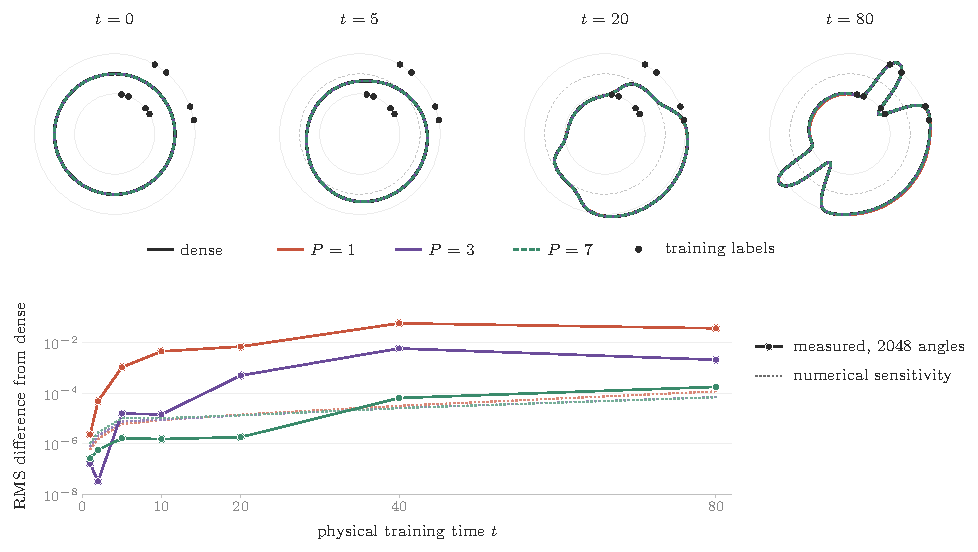
\includegraphics[width=\textwidth]{figures/trajectory.pdf}
 \caption{\textbf{A trajectory, not only an endpoint.}
 Existing paired-label circle experiment: two hidden tanh layers,
 width $2048$, and Legendre orders $q=1,3,7$. Predictions are saved at
 the same physical times $t=0,5,20,80$. Radius is $3+f(\theta)$, the
 dashed ring marks zero, and black points are training labels.
 The source replay records $39$ common times and uses float64 adaptive
 Heun integration at two tolerances. These are discrete observations,
 not a certificate between the saved times.}
 \label{fig:trajectory}
\end{figure}
\begin{figure}[t]
 \centering
 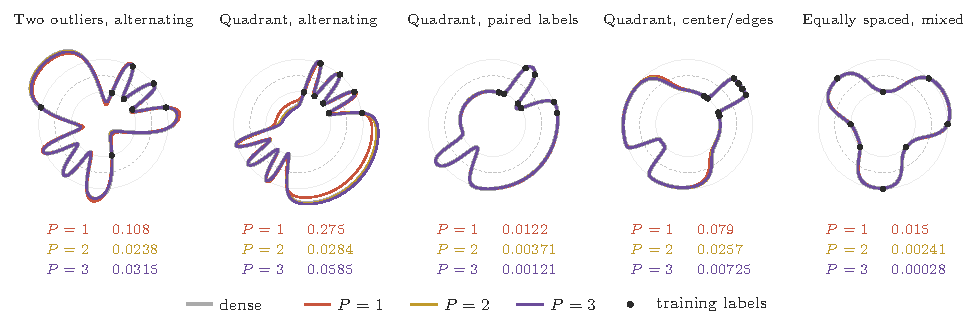
\includegraphics[width=\textwidth]{figures/circles_deep.pdf}
 \caption{\textbf{Fitted functions on unseen inputs.}
 Existing five-task comparison: three hidden tanh layers, width $4096$,
 and Legendre orders $q=1,2,3$, at each model's own training-MSE
 $10^{-3}$ endpoint, not a shared time. Grey curves are dense predictions,
 coloured curves are memory predictions, and black points are labels.
 Printed discrepancies are RMS differences on $8192$ circle queries,
 not uniform errors or risk against unseen labels. Fixed initialized
 matrices remain additional to Legendre's moving state.}
 \label{fig:deep}
\end{figure}
The first panel tests tracking the developing function; the second tests
selection of a fitted function away from the labels. Neither establishes
a universal ordering of small memory budgets. Portable source bundles,
renderers and capture commands remain with the paper. This revision
reuses the recorded figures without rerunning training.
\FloatBarrier

\section{Related work and discussion}
\label{sec:related}
The comparison is between representations of a specified learning process,
not a claim that other descriptions lack quantitative guarantees.
Tensor Programs and multilayer mean-field theory provide feature-learning
population frameworks \citep{yang2021tensor,nguyen2023rigorous};
dynamical mean-field descriptions organize temporal correlations and
responses \citep{bordelon2022dmft,bordelon2023finite}. Model assumptions,
observables and solver representations must be matched before comparing
their resource costs. Our certificates concern finite Gaussian networks,
all physical times and the whole passive-input sphere.

A frozen neural tangent kernel describes a different limiting regime
\citep{jacot2018ntk,lee2019wide}. Higher-order responses appear in the neural
tangent hierarchy \citep{huang2020nth}, whose truncation theorem has its
own scaling and horizon. Online polynomial memory summarizes an externally
given signal \citep{gu2020hippo}; here the signals are endogenous, generated
by the network reconstructed from those memories. Stabilizing that
feedback is an additional obligation. The appendix also supplies the
finite-space generator and numerical conditioning arguments used by the
decoder; no fresh-noise approximation replaces a reused trained matrix.

\paragraph{The trade-off is not one-dimensional.}
Legendre makes the evolving memory small but retains a quadratic fixed
environment. Harmonic removes that environment from the retained state
and has polylogarithmic query work at fixed dimension, with near-linear
implicit setup. The decoder has a dimension-independent logarithmic
word-storage exponent, but regenerates width-many rows per query and
matches an independent dense run only at its upper-certificate scale.

\paragraph{Open boundaries.}
The dense lower bound is transient and does not establish sharp
sample/gap dependence. Small labels are a sufficient stability regime,
not a sharp necessity or a width-dependent scaling.
The analytic class includes unbounded values but not exact ReLU.
Exact-real setup costs do not establish fixed-machine-precision performance
or superiority at practical widths. Finite-word costs charge activation
and external-data access explicitly. Finally, trajectory fidelity alone
does not establish out-of-sample label risk: the usefulness of the
selected predictor remains a separate question.

\bibliographystyle{plainnat}
\bibliography{references}
\clearpage
\appendix
\section*{Guide to the detailed statements and proofs}
\addcontentsline{toc}{section}{Guide to the detailed statements and proofs}
The appendices contain the complete parameter-explicit scientific statement
and proof chain. The main text suppresses activation/depth factors and
normalizes prediction error by $Y$. An absolute-error tolerance in the
detailed certificates is therefore evaluated at $Y\varepsilon$ for the
main text's normalized target. The appendix restores activation/depth
coefficients explicitly; its numerical $C$ is distinguished from the
activation/depth envelope denoted by $C$ in the main text.
Here $A=W^{(1)}$ when the first layer
is written separately, and $w$ is the same output weight as above.
Local proof constants, source degrees and numerical orders are not new
runtime model parameters.

The full label, width, confidence, storage and cost interfaces are followed
by numerical certificates and proofs. The shared source construction,
both efficient Harmonic initializers, and the finite decoder are included
in the manuscript itself, not left as dependencies on research notes.
Historical review records and superseded paper theorems are not premises.

\medskip
\noindent\begin{tabularx}{\textwidth}{@{}Xr@{}}
\toprule
Detailed component & Page\\
\midrule
\hyperref[int:headline-results]{Complete certificate interfaces and notation}
& \pageref{int:headline-results}\\
\hyperref[int:detailed-statements]{Explicit statements, constants and cost inventories}
& \pageref{int:detailed-statements}\\
\hyperref[int:source-foundations]{Shared source construction and analytic estimates}
& \pageref{int:source-foundations}\\
\hyperref[int:dense-proofs]{Dense upper and lower bounds}
& \pageref{int:dense-proofs}\\
\hyperref[int:legendre-proofs]{Legendre construction and all-order comparison}
& \pageref{int:legendre-proofs}\\
\hyperref[int:harmonic-proofs]{Harmonic geometry, stability and budget inversion}
& \pageref{int:harmonic-proofs}\\
\hyperref[int:logarithmic-decoder-proofs]{Logarithmic decoder and confidence bounds}
& \pageref{int:logarithmic-decoder-proofs}\\
\hyperref[int:decoder-finite-construction]{Finite source, numerical execution and word backend}
& \pageref{int:decoder-finite-construction}\\
\hyperref[int:harmonic-efficient-setup-proofs]{Explicit and implicit Harmonic initialization}
& \pageref{int:harmonic-efficient-setup-proofs}\\
\bottomrule
\end{tabularx}

\begingroup
\small
% Static scientific appendix. Generated from RESULT.md SHA256 9c7b10dda810c13384ba9c85ffa70ca72b2be2475a7400377db028cf169f77f4.
% Rebuild: node studies/integrated_general_compression_20261004/paper_appendix_build.mjs --check
% Required packages: amsmath, amssymb, mathtools, mathrsfs, graphicx, array, booktabs, longtable, hyperref.
% No study file is read by LaTeX. Source line comments and build manifest audit coverage.
\providecommand{\inttablemath}[1]{\begingroup
  \setbox0=\hbox{$\textstyle #1$}%
  \ifdim\wd0>\linewidth\typeout{INTTABLE:\the\inputlineno:\the\wd0:\the\linewidth}\fi
  \ifdim\wd0>\linewidth\resizebox{\linewidth}{!}{\box0}\else\box0\fi
  \endgroup}
\providecommand{\intdisplay}[1]{\begingroup
  \setbox0=\hbox{$\displaystyle #1$}%
  \dimen0=\dimexpr\linewidth-5em\relax
  \ifdim\wd0>\dimen0\typeout{INTDISPLAY:\theHequation:\the\wd0:\the\dimen0}\fi
  \ifdim\wd0>\dimen0\resizebox{\dimen0}{!}{\box0}\else\box0\fi
  \endgroup}
\clearpage


% SOURCE 276--276: heading
\section{Complete certificate interfaces and notation}
\label{int:headline-results}


The first-layer matrix denoted by \(A\) in the detailed formulas below is
exactly \(W^{(1)}\) in the main text. The hidden matrices
\(W^{(2)},\ldots,W^{(L)}\), readout \(w\), physical time, and all
normalizations are unchanged. In particular, \(h^{(0)}=x/\sqrt d\),
and the prediction is \(w^\top h^{(L)}/n\). This correspondence avoids
changing proof-local notation or introducing a second model.


% SOURCE 278--278: heading
\subsection{Shared setup, notation and qualifications}


% SOURCE 280--292: paragraph

The structural parameters remain separate: dense width \(n\), sample count \(m\), input dimension \(d\), and hidden depth \(L\ge2\). Inputs satisfy \(\|x_a\|_2=\sqrt d\), and labels are arbitrary fixed real numbers. The common freely supplied compression order is \(q\): Legendre memory order or Harmonic per-layer neuron budget. Logarithmic decoder compression has no free \(q\); its moment and field orders are prescribed by the width, problem and confidence certificate. The remaining global numerical symbols are label RMS \(Y\), feature gap \(\gamma\), activation envelope \(\beta\), failure probability \(\delta\), target accuracy \(\varepsilon\), and a generic numerical constant \(C\). Different occurrences of \(C\) may denote different universal constants; they never conceal structural dependence. The detailed statements and proofs use locally defined coefficients, not extra model orders.


% SOURCE 294--294: paragraph

The dense forward pass is


% SOURCE 295--299: display
\begingroup\renewcommand{\theHequation}{intdisplay.1}
\begin{equation*}
\intdisplay{
z^{(1)}=Ax/\sqrt d,\qquad
z^{(j)}=W^{(j)}h^{(j-1)},\qquad h^{(j)}=\phi_j(z^{(j)}),
\qquad f_n=w^\top h^{(L)}/n.
}
\end{equation*}
\endgroup

% SOURCE 300--311: paragraph

The first weights have independent \(N(0,\allowbreak 1)\) entries; hidden mixers have independent \(N(0,\allowbreak 1/n)\) entries; blocks are independent; \(w(0)=0\). Training minimizes mean squared loss with mobilities \((n,\allowbreak 1,\allowbreak \ldots,\allowbreak 1,\allowbreak n)\). The dense copy \(\widetilde f_n\) is independently initialized. Legendre and Harmonic use their realized reference initialization and the same physical time; the Logarithmic decoder instead compares a newly generated compressed model with an independent dense reference. For the implicit Harmonic initializer, that realization is latent: exact adaptive Gaussian actions couple the output to one ordinary dense reference without generating its full hidden matrices. This samples a fresh joint reference/output law; it is not conversion of a previously supplied matrix or a prescribed entrywise random seed.


% SOURCE 313--315: paragraph

Each activation is real on the real axis, holomorphic on a common strip \(|\operatorname{Im}z|<a\), with bounded first derivative there. Activation values may be unbounded. Set


% SOURCE 316--320: display
\begingroup\renewcommand{\theHequation}{intdisplay.2}
\begin{equation*}
\intdisplay{
\beta=\max\left\{10,1+\max_j|\phi_j(0)|,\frac{16}{a},
\max_{j,\,k\in\{1,2\}}\sup_{|\operatorname{Im}z|\le a/2}
|\phi_j^{(k)}(z)|\right\},\qquad Y=\frac{\|y\|_2}{\sqrt m}.
}
\end{equation*}
\endgroup

% SOURCE 321--321: paragraph

The covariance recursion and unweighted gap are


% SOURCE 322--327: display
\begingroup\renewcommand{\theHequation}{intdisplay.3}
\begin{equation*}
\intdisplay{
Q^{(0)}_{ab}=x_a^\top x_b/d,\qquad
Q^{(j)}_{ab}=\mathbb E[\phi_j(Z_a)\phi_j(Z_b)],\quad
Z\sim N(0,Q^{(j-1)}),\qquad
\gamma=\lambda_{\min}(Q^{(L)})>0.
}
\end{equation*}
\endgroup

% SOURCE 328--331: paragraph

The gap is not divided by \(m\). No orthogonality, centering, sign pattern or clipping is imposed. Dense, Legendre and Harmonic need no input-rank assumption. Only the Logarithmic decoder uses the already stated spanning condition and \(m\ge d\).


% SOURCE 333--334: paragraph

\textbf{Labels.} The clean dense/Legendre envelopes below use the unchanged sufficient cap


% SOURCE 335--338: display
\begingroup\renewcommand{\theHequation}{intdisplay.4}
\begin{equation}
\intdisplay{
0<Y\le\frac\gamma m\beta^{-30L}.
}
\label{int:eq-0001-labels}
\end{equation}
\endgroup

% SOURCE 339--342: paragraph

The larger original recurrence allowance is retained explicitly at the start of \hyperref[int:detailed-statements]{the detailed statements}. The Harmonic forward theorem and its new beta-only storage envelope hold on that entire larger range. Zero labels give the stationary zero predictor and exact constant-zero compression separately.


% SOURCE 344--344: paragraph

\textbf{Error.} All comparisons use


% SOURCE 345--349: display
\begingroup\renewcommand{\theHequation}{intdisplay.5}
\begin{equation}
\intdisplay{
\|f-g\|_*=
\sup_{t\in[0,\infty]}\sup_{\|x\|_2=\sqrt d}|f(t,x)-g(t,x)|.
}
\label{int:eq-0002-norm}
\end{equation}
\endgroup

% SOURCE 350--351: paragraph

This includes fitted limits and the whole sphere, a circle only when \(d=2\). It measures function fidelity, not unknown-label test risk.


% SOURCE 353--367: paragraph

\textbf{Probability and width.} Fix \(0<\delta<1\). For the dense, Legendre and Harmonic results, each fixed admissible problem has a finite width threshold, depending on all its parameters and \(\delta\), above which the stated comparisons hold jointly with probability at least \(1-\delta\). It includes inherited source/initialization gates, the lower theorem's eventual threshold when used, and the explicit \hyperref[int:harmonic-storage-count]{analytic-tail and construction gates}. Its stochastic part remains unquantified. Logarithmic decoder compression has instead the explicit, extremely conservative sufficient width stated below; it introduces no additional existential stochastic threshold. Every statement concerns each individual width, not one event over infinitely many independent initializations. Split failure budgets for joint statements. Fixed-confidence logarithms in the first three upper bounds are absorbed by their eventual-width convention, not by a claimed numerical failure-rate formula. Multiplying storage by a fixed constant is not claimed to produce exponential confidence amplification.


% SOURCE 369--379: paragraph

\textbf{Model domains.} Legendre permits every integer \(q\ge1\), with no separate accuracy-order condition. The Harmonic family permits every integer budget \(q\ge18(2m+d+9)\), abbreviated \(q\ge C(m+d)\) in the headline counts only. This is exact-initialization overhead: positive training Gram forces top width at least \(m\), and exact first-weight columns force first width at least \(d\) when \(n\ge d\). For \(q\ge n\), the full selected space gives exact agreement with dense. Logarithmic decoder compression instead requires \(m\ge d\), spanning training inputs, \(0<\delta<1/4\), and the complete common fitting/source label allowance. It is a certificate-prescribed family indexed by \(n\), not an arbitrary-budget family indexed by \(q\).


% SOURCE 381--381: heading
\subsection{Forward interface: supplied size/order gives storage and error}


% SOURCE 383--388: paragraph

Dense, Legendre and Harmonic storage counts real coordinates, not bits. Logarithmic decoder storage counts finite numerical words and states its certified bits per word separately. The separate \hyperref[int:computational-costs]{computational-cost section} reports initialization, per-stage training and single-query costs; storage alone is not a runtime bound. For \(n\ge d\), the clean counts are:


% SOURCE 390--395: table
\begingroup\small
\setlength{\LTleft}{0pt}\setlength{\LTright}{0pt}
\renewcommand{\arraystretch}{1.2}
\begin{longtable}{@{}>{\raggedright\arraybackslash}p{0.25\linewidth}>{\raggedright\arraybackslash}p{0.71\linewidth}@{}}
\toprule
\multicolumn{2}{@{}l@{}}{\textit{Detailed comparison}} \\ \midrule
\endhead
\multicolumn{2}{@{}p{0.96\linewidth}@{}}{\textbf{Model: Dense}} \\
Learned state & \inttablemath{O(Ln^2)} \\
All retained model storage & \inttablemath{O(Ln^2)} \\
\addlinespace[0.45em]
\multicolumn{2}{@{}p{0.96\linewidth}@{}}{\textbf{Model: Legendre}} \\
Learned state & \inttablemath{O(n[d+Lmq])} \\
All retained model storage & \inttablemath{O(Ln^2+Lmnq)} \\
\addlinespace[0.45em]
\multicolumn{2}{@{}p{0.96\linewidth}@{}}{\textbf{Model: Harmonic}} \\
Learned state & \inttablemath{O(Lq^2)} \\
All retained model storage & \inttablemath{O(Lq^2)} \\
\addlinespace[0.45em]
\multicolumn{2}{@{}p{0.96\linewidth}@{}}{\textbf{Model: Logarithmic decoder}} \\
Learned state & bounded by the complete-model envelope at right \\
All retained model storage & \inttablemath{O(\log^6(en)\log\log(e^e+n))} numerical words at fixed problem parameters \\
\addlinespace[0.45em]
\bottomrule
\end{longtable}
\endgroup

% SOURCE 397--407: paragraph

Before simplification, the exact dense moving count is \((L-1)n^2+n(d+1)\), the Legendre count is \(n(d+1)+1+2(L-1)mnq\), and Harmonic has at most \((L-1)q^2+q(d+1)+m\). Legendre additionally retains \((L-1)n^2\) fixed mixers; reconstructed matrices are evaluation objects. Harmonic includes metrics, fixed copies, residual coordinates, data and solve caches. Original-width source arrays and jets are discarded. Ordinary data storage is additional for the dense/Legendre model-state counts if retained. The Logarithmic decoder count already includes its normalized training table, all ensemble members, seeds, selected packets, caches and current scalar state.


% SOURCE 409--412: paragraph

Legendre uses its original residual-RMS clock and prefixes. Harmonic uses the corrected-readout autonomous optimizer, not ordinary gradient flow on an arbitrary smaller network. All hidden arrays train. Neither has a second independent runtime approximation order.


% SOURCE 414--414: heading
\subsubsection{Dense versus an independent dense copy}


% SOURCE 416--416: paragraph

A simplified polynomial upper envelope is


% SOURCE 417--422: display
\begingroup\renewcommand{\theHequation}{intdisplay.6}
\begin{equation}
\intdisplay{
\|f_n-\widetilde f_n\|_*
\le C\beta^{CL}Y\left(1+\frac m\gamma\right)^5
\sqrt{\frac dn}\,\log(en)e^{\sqrt{\log(en)}}.
}
\label{int:eq-0003-dense-upper}
\end{equation}
\endgroup

% SOURCE 423--425: paragraph

The exact, sharper actual-label coefficient and confidence logarithm remain in \hyperref[int:dense-forward-comparison]{the exact dense certificate}. The sample/gap powers in this upper envelope are not claimed sharp.


% SOURCE 427--427: paragraph

For \(m\ge2\),


% SOURCE 428--433: display
\begingroup\renewcommand{\theHequation}{intdisplay.7}
\begin{equation}
\intdisplay{
\|f_n-\widetilde f_n\|_*
\ge c_{\phi,L,\delta}\frac{Y\sqrt\gamma}
{\sqrt n\,\log(en)^{5/2}}.
}
\label{int:eq-0004-dense-lower}
\end{equation}
\endgroup

% SOURCE 434--439: paragraph

The positive coefficient depends only on activations, depth and confidence; its formula is in \hyperref[int:dense-trajectory-lower]{the exact lower theorem}. It cannot be replaced by a confidence-independent universal constant. The actual-prediction witness occurs at a positive early time, possibly shrinking with width; this is not an endpoint lower bound. Deterministic exceptions prevent the general assertion at \(m=1\).


% SOURCE 441--441: heading
\subsubsection{Legendre versus its realized dense reference}


% SOURCE 443--443: paragraph

For every integer \(q\ge1\),


% SOURCE 444--450: display
\begingroup\renewcommand{\theHequation}{intdisplay.8}
\begin{equation}
\intdisplay{
\|f_{\mathrm{Leg},n,q}-f_n\|_*
\le C\beta^{CL}Y\left(1+\frac m\gamma\right)^6
\frac{\sqrt{\log(en)\log(eq)}}{q^2}
e^{\sqrt{\log(en)}}.
}
\label{int:eq-0005-legendre-forward}
\end{equation}
\endgroup

% SOURCE 451--456: paragraph

The stronger exact actual-label coefficient is unchanged: \hyperref[int:legendre-forward-certificates]{the exact all-order statement}. Above the actual absorption threshold use the signed comparison; below it use the all-order fitting/predictor bound. Retaining the small label powers shows that the same coefficient covers both regions. No second error term or accuracy-order gate is needed on the explicit cap.


% SOURCE 458--458: heading
\subsubsection{Harmonic versus its realized dense reference}


% SOURCE 460--460: paragraph

For every Harmonic budget in the shared model domain,


% SOURCE 461--470: display
\begingroup\renewcommand{\theHequation}{intdisplay.9}
\begin{equation}
\intdisplay{
\begin{aligned}
\|f_{\mathrm{Harm},n,q}-f_n\|_*
\le{}&C\beta^{CL}Y\frac m\gamma
\left(1+\sqrt{\frac m\gamma}\right)n e^{C\sqrt{\log(en)}}\\
&\times\exp\left[-\frac{\sqrt d}{C\beta^{CL}}
\left(\frac{q}{(Ym/\gamma)^2\log(en)^{d/2}}\right)^{1/(d+1)}\right].
\end{aligned}
}
\label{int:eq-0006-harmonic-forward}
\end{equation}
\endgroup

% SOURCE 471--477: paragraph

This is a genuine decreasing certificate in supplied \(q\). The construction takes \(n,\allowbreak q\) as inputs; its internal source tolerance and horizon are determined by the budget and discarded after setup. There is no fixed error floor. For \(q\ge n\), exact retention improves the bound to zero. The growing comparison exponential has only numerical coefficient \(C\); structural factors in the negative exponential specify approximation efficiency, not unstable amplification.


% SOURCE 479--483: paragraph

The power \(1/(d+1)\) comes from approximating the sphere and a horizon that grows with required accuracy. It is a construction rate, not an optimality lower bound. An initialization-only selected model covers smaller budgets within the shared domain using independent fitting; there is no hidden extra accuracy-dependent budget test.


% SOURCE 485--490: paragraph

The original construction at source tolerance \(1/n\) remains valid with its sharper error \(C\beta^{CL}Y(m/\gamma)(1+\sqrt{m/\gamma}) n^{-1}e^{C\sqrt{\log(en)}}\) and original \(O(\log(en)^{3d+2})\) all-retained storage. The supplied-budget family preserves that specialization as a separate available construction.


% SOURCE 493--493: heading
\subsubsection{Logarithmic decoder versus an independent dense reference}
\label{int:logarithmic-forward-interface}

% SOURCE 495--496: paragraph

This method has no supplied order \(q\). Define its implemented member moment order and common resource logarithm by


% SOURCE 497--505: display
\begingroup\renewcommand{\theHequation}{intdisplay.10}
\begin{equation}
\intdisplay{
p=\max\left\{1,\left\lceil
\frac{\log(2^{22}emL)}{\log(64e^2)}
\right\rceil\right\},
\qquad
Z=\log(en)+\log\left(e+
\frac{(m+d+2)\beta^{100L}(1+m/\gamma)}\delta\right).
}
\label{int:eq-0007-logarithmic-decoder-orders}
\end{equation}
\endgroup

% SOURCE 506--506: paragraph

The confidence-dependent order used only to certify the independent reference is


% SOURCE 507--512: display
\begingroup\renewcommand{\theHequation}{intdisplay.11}
\begin{equation}
\intdisplay{
p_{\rm ref}=\max\left\{1,\left\lceil
\frac{\log(2^{22}emL/\delta)}{\log(64e^2)}
\right\rceil\right\}.
}
\label{int:eq-0008-logarithmic-reference-order}
\end{equation}
\endgroup

% SOURCE 513--513: paragraph

A sufficient enclosing width is


% SOURCE 514--522: display
\begingroup\renewcommand{\theHequation}{intdisplay.12}
\begin{equation}
\intdisplay{
n\ge\max\left\{
C_*\left[
\frac{2^{20}\beta^{2000L}(1+m/\gamma)^4
(m+d+p_{\rm ref}+1)^4}{\delta}
\right]^{1100},\;Y^{-1},\;C_{\rm num}
\right\}.
}
\label{int:eq-0009-logarithmic-explicit-width}
\end{equation}
\endgroup

% SOURCE 523--528: paragraph

Here \(C_*\) is universal and \(C_{\rm num}=\max\{1,\allowbreak (A_{\rm num}/32)^{1/9}\}\), where \(A_{\rm num}\) is the absolute coefficient in the chosen numerical-error allocation. The sharper factorized gate and the few separately displayed implementation gates are retained in \hyperref[int:detailed-statements]{the detailed-statement appendix}. This width is fully quantitative but extremely conservative.


% SOURCE 530--530: paragraph

Let


% SOURCE 531--541: display
\begingroup\renewcommand{\theHequation}{intdisplay.13}
\begin{equation}
\intdisplay{
\begin{aligned}
b_n={}&\frac{c_0Y}{\sqrt n}
e^{c_1Y^2\sqrt{\log(en)}}
\sqrt{8\log\frac{2048(n+1)(1+2n)^d}{\delta}}
+c_{2,\rm mesh}\frac Yn,\\
&32\le c_{2,\rm mesh}\le
C\beta^{4L}(1+m/\gamma).
\end{aligned}
}
\label{int:eq-0010-logarithmic-dense-certificate}
\end{equation}
\endgroup

% SOURCE 542--544: paragraph

The positive coefficients \(c_0,\allowbreak c_1\) are the inherited fixed-problem coefficients of the dense comparison; this construction does not quantify them further. At every width satisfying the stated gates,


% SOURCE 545--548: display
\begingroup\renewcommand{\theHequation}{intdisplay.14}
\begin{equation}
\intdisplay{
\|f_{\rm Log,n}-f_n^{\rm ind}\|_*\le3b_n
}
\label{int:eq-0011-logarithmic-forward}
\end{equation}
\endgroup

% SOURCE 549--552: paragraph

with probability at least \(1-\delta\). The event is simultaneous over all sphere inputs, all physical times, adaptively chosen queries, and the fitted endpoint. The compact model is built jointly with a fresh independent dense reference law; it does not encode a previously supplied dense matrix or seed.


% SOURCE 554--554: paragraph

Its learned and total retained storage are both at most a universal multiple of


% SOURCE 555--559: display
\begingroup\renewcommand{\theHequation}{intdisplay.15}
\begin{equation}
\intdisplay{
p^2\beta^{402L}(m+d+2)^2(1+m/\gamma)^2Z^6
\bigl[d+1+\log(e+(d+1)Z)\bigr]
}
\label{int:eq-0012-logarithmic-word-storage}
\end{equation}
\endgroup

% SOURCE 560--565: paragraph

numerical words, each of sufficient length \(C\beta^{110L}Z\) bits. This includes all retained data, seeds and members; the same word envelope also covers the live query workspace. The clean display uses \(nY\ge1\), already enforced by the width gate. For \(0<nY<1\), replace \(Z\) everywhere in the numerical counts by \(Z+\log_+(1/(nY))\) and retain the enlarged Gaussian-RMS gate.


% SOURCE 567--569: paragraph

This method reaches the dense-pair upper-certificate scale, not the Harmonic method's stronger matched-reference \(n^{-1+o(1)}\) error. In particular its error divided by the actual dense discrepancy is not proved to vanish.


% SOURCE 572--572: heading
\subsubsection{Two efficient initializers for the same Harmonic family}
\label{int:harmonic-setup-headline}

% SOURCE 574--579: paragraph

The source coefficients can be constructed either by \textbf{explicit dense local continuation} or by \textbf{implicit Gaussian local continuation}. Both preserve the full original label interval, activation class, confidence event, prediction certificates, retained-state inventory and autonomous optimizer. Neither changes the final model's physical time zero. The original finite initialization-jet construction remains a valid, separately costed alternative.


% SOURCE 581--583: paragraph

At source tolerance \(1/n\) and source horizon \(32(m/\gamma)\log(en)\), with each admissible structural parameter and confidence fixed separately, their sufficient bounds are:


% SOURCE 585--588: table
\begingroup\small
\setlength{\LTleft}{0pt}\setlength{\LTright}{0pt}
\renewcommand{\arraystretch}{1.2}
\begin{longtable}{@{}>{\raggedright\arraybackslash}p{0.25\linewidth}>{\raggedright\arraybackslash}p{0.71\linewidth}@{}}
\toprule
\multicolumn{2}{@{}l@{}}{\textit{Detailed comparison}} \\ \midrule
\endhead
\multicolumn{2}{@{}p{0.96\linewidth}@{}}{\textbf{Harmonic initializer: Explicit dense local continuation}} \\
Setup work & \inttablemath{O(n^2\log(en)^{3d/2+1})} \\
Peak setup memory & \inttablemath{O(n^2)} \\
\addlinespace[0.45em]
\multicolumn{2}{@{}p{0.96\linewidth}@{}}{\textbf{Harmonic initializer: Implicit Gaussian local continuation}} \\
Setup work & \inttablemath{O(n\log(en)^{9d/2+3})} \\
Peak setup memory & \inttablemath{O(n\log(en)^{3d/2+1})} \\
\addlinespace[0.45em]
\bottomrule
\end{longtable}
\endgroup

% SOURCE 590--596: paragraph

Both retain \(O(\log(en)^{3d+2})\) coordinates and the same stronger \(n^{-1+o(1)}\) whole-sphere/all-time error. These headline setup rows assume bounded-cost scalar activation, elementary-function and Gaussian primitives. The \hyperref[int:harmonic-efficient-initialization]{finite supplied-order formulas} and \hyperref[int:harmonic-efficient-orders]{complete parameter recipe} expose all \(m,\allowbreak d,\allowbreak L,\allowbreak \gamma,\allowbreak Y,\allowbreak \beta\), order and primitive-cost dependence; it is not suppressed in a universal constant.


% SOURCE 598--605: paragraph

Here a computationally cheap rollout reconstructs the required physical interval using restarted high-order local expansions. It is not a claim that an arbitrary short initial-time prefix suffices, or that a fixed number of ordinary Euler steps supplies the coefficients. The implicit method samples exactly the joint law of the explicit finite local initializer and its dense reference; it need not return the identical finite coefficient approximations of the older origin-jet algorithm. No dense array, query oracle, or setup history remains in either final compressed model.


% SOURCE 607--607: heading
\subsection{Inverse interface: supplied accuracy determines size/order}


% SOURCE 609--609: paragraph

The common target is


% SOURCE 610--613: display
\begingroup\renewcommand{\theHequation}{intdisplay.16}
\begin{equation}
\intdisplay{
\mathbb P\{\|f_{\rm model}-f_n\|_*\le\varepsilon\}\ge1-\delta.
}
\label{int:eq-0013-target}
\end{equation}
\endgroup

% SOURCE 614--618: paragraph

For each certificate choose the smallest permitted integer size/order whose right side is at most \(\varepsilon\), with the common width gates enforced. This minimizes the increasing storage-budget bound within that certificate, not compression among all possible models. Exact scalar inversions, including loose targets and the full-width fallback, are in \hyperref[int:detailed-statements]{the detailed-statement appendix}.


% SOURCE 620--628: paragraph

The following simpler prescriptions describe polynomial accuracy \(\varepsilon=n^{-\Theta(1)}\), with structural parameters and confidence fixed and \(n\) sufficiently large: the accuracy may lie between two different fixed negative powers of \(n\), not necessarily \(1/n\). This does not identify or order \(m,\allowbreak d,\allowbreak L,\allowbreak 1/\gamma\). The common eventual convention absorbs fixed coefficients inside logarithms. For the user's large-parameter simplification use \(m/\gamma\ge1\); otherwise replace that ratio by \(1+m/\gamma\) in the dense/Legendre prescriptions.


% SOURCE 630--630: heading
\subsubsection{Dense: choose width before initialization}


% SOURCE 632--632: paragraph

A sufficient eventual choice is


% SOURCE 633--641: display
\begingroup\renewcommand{\theHequation}{intdisplay.17}
\begin{equation}
\intdisplay{
n=\left\lceil
\frac{C\beta^{CL}Y^2d}{\varepsilon^2}
\left(1+\frac m\gamma\right)^{10}
\log(e/\varepsilon)^2
e^{C\sqrt{\log(e/\varepsilon)}}\right\rceil,
\qquad \text{storage}=O(Ln^2).
}
\label{int:eq-0014-dense-inverse}
\end{equation}
\endgroup

% SOURCE 642--642: paragraph

Its all-retained model storage has the explicit sufficient envelope


% SOURCE 643--649: display
\begingroup\renewcommand{\theHequation}{intdisplay.18}
\begin{equation}
\intdisplay{
\operatorname{storage}(\widetilde f_n)\le
CL\beta^{CL}Y^4d^2\left(1+\frac m\gamma\right)^{20}
\varepsilon^{-4}\log(e/\varepsilon)^4
e^{C\sqrt{\log(e/\varepsilon)}}.
}
\label{int:eq-0015-dense-inverse-storage}
\end{equation}
\endgroup

% SOURCE 650--654: paragraph

This is eventual as \(\varepsilon\downarrow0\): the selected width must exceed the common threshold. It is not a fully effective confidence-certified width, because the stochastic source threshold is unquantified. It selects a reference before initialization, not a replacement for an already prescribed reference.


% SOURCE 656--656: heading
\subsubsection{Legendre: choose order for the given reference}


% SOURCE 658--658: paragraph

The inverse of the forward bound has sufficient eventual form


% SOURCE 659--665: display
\begingroup\renewcommand{\theHequation}{intdisplay.19}
\begin{equation}
\intdisplay{
q=\left\lceil C\beta^{CL}\left(\frac m\gamma\right)^3
\sqrt{\frac Y\varepsilon}\,
[\log(en)\log(en/\varepsilon)]^{1/4}
e^{\frac12\sqrt{\log(en)}}\right\rceil.
}
\label{int:eq-0016-legendre-inverse}
\end{equation}
\endgroup

% SOURCE 666--666: paragraph

Consequently


% SOURCE 667--674: display
\begingroup\renewcommand{\theHequation}{intdisplay.20}
\begin{equation}
\intdisplay{
\text{learned storage}\le Cnd+
C\beta^{CL}Lmn\left(\frac m\gamma\right)^3
\sqrt{\frac Y\varepsilon}\,
[\log(en)\log(en/\varepsilon)]^{1/4}
e^{\frac12\sqrt{\log(en)}}.
}
\label{int:eq-0017-legendre-inverse-storage}
\end{equation}
\endgroup

% SOURCE 675--680: paragraph

Fixed mixers remain additional. There is no separate order-admissibility test even before taking this eventual simplification. Keeping the two logarithms also keeps the coefficient uniform in the fixed polynomial accuracy exponent; replacing them by \(\log(en)^2\) would hide a constant depending on that exponent. At the absolute root-width target \(\varepsilon=n^{-1/2}\), this gives


% SOURCE 681--686: display
\begingroup\renewcommand{\theHequation}{intdisplay.21}
\begin{equation}
\intdisplay{
\text{learned storage}\le Cnd+
C\beta^{CL}Lm\sqrt Y\left(\frac m\gamma\right)^3n^{5/4}
\sqrt{\log(en)}e^{\frac12\sqrt{\log(en)}}.
}
\label{int:eq-0018-legendre-absolute-root-width-storage}
\end{equation}
\endgroup

% SOURCE 687--690: paragraph

The outer factor \(m\) is the response-memory multiplicity in the exact count \(n(d+1)+1+2(L-1)mnq\); it has not been removed. When \(m\ge d\) and the positive problem parameters are fixed while \(n\) grows, the second term eventually dominates \(nd\), and the clean form is


% SOURCE 691--696: display
\begingroup\renewcommand{\theHequation}{intdisplay.22}
\begin{equation}
\intdisplay{
\text{learned storage}
\le C\beta^{CL}Lm\sqrt Y
\left(\frac m\gamma\right)^3n^{5/4+o(1)}.
}
\label{int:eq-0019-legendre-simplified-root-width-learned-storage}
\end{equation}
\endgroup

% SOURCE 697--700: paragraph

At the label-scaled root target \(\varepsilon=Y/\sqrt n\), used before the extra logarithmic enlargement that makes compression negligible relative to dense variability, the factor \(\sqrt Y\) cancels. Thus, under the same \(m\ge d\) convention,


% SOURCE 701--705: display
\begingroup\renewcommand{\theHequation}{intdisplay.23}
\begin{equation}
\intdisplay{
\text{learned storage}
\le C\beta^{CL}Lm\left(\frac m\gamma\right)^3n^{5/4+o(1)}.
}
\label{int:eq-0020-legendre-dense-variability-scale-learned-storage}
\end{equation}
\endgroup

% SOURCE 707--707: heading
\subsubsection{Harmonic: choose width budget for the given reference}


% SOURCE 709--709: paragraph

Inverting its stretched-exponential certificate gives


% SOURCE 710--716: display
\begingroup\renewcommand{\theHequation}{intdisplay.24}
\begin{equation}
\intdisplay{
q=\left\lceil C(m+d)+
\frac{\beta^{C(d+1)L}}{d^{(d+1)/2}}
\left(\frac{Ym}{\gamma}\right)^2
\log(en)^{d/2}\log(en/\varepsilon)^{d+1}\right\rceil.
}
\label{int:eq-0021-harmonic-inverse}
\end{equation}
\endgroup

% SOURCE 717--717: paragraph

The corresponding all-retained bound, hence also the learned-state bound, is


% SOURCE 718--725: display
\begingroup\renewcommand{\theHequation}{intdisplay.25}
\begin{equation}
\intdisplay{
\operatorname{storage}(f_{\mathrm{Harm},n,q})
\le CL(m+d)^2+
\frac{L\beta^{C(d+1)L}}{d^{d+1}}
\left(\frac{Ym}{\gamma}\right)^4
\log(en)^d\log(en/\varepsilon)^{2d+2}.
}
\label{int:eq-0022-harmonic-inverse-storage}
\end{equation}
\endgroup

% SOURCE 726--730: paragraph

There is no factorial ratio: Stirling bounds \((d+3)^d/(d!)^2\) by \(C^{d+1}/d^{d+1}\), and numerical powers are absorbed in the displayed activation-depth envelope. At polynomial accuracy this is \(O(\log(en)^{3d+2})\) for fixed structural parameters, preserving the previous qualitative storage order.


% SOURCE 732--734: paragraph

For an arbitrary target outside that regime, keep the unshortened logarithm from the forward certificate: replace \(\log(en/\varepsilon)\) in the sufficient budget by


% SOURCE 735--739: display
\begingroup\renewcommand{\theHequation}{intdisplay.26}
\begin{equation}
\intdisplay{
\log(en)+\log\left(e+
\frac{C\beta^{CL}Y(m/\gamma)(1+\sqrt{m/\gamma})}{\varepsilon}\right).
}
\label{int:eq-0023-harmonic-inverse-logarithm}
\end{equation}
\endgroup

% SOURCE 740--744: paragraph

Enlarging numerical constants absorbs \(\sqrt{\log(en)}\). If the sufficient budget exceeds \(n\), the exact full-width branch suffices instead. The exact inverse in the proof also handles targets already met by the initialization-only model. These are internal choices of one width budget, not extra runtime orders.


% SOURCE 746--746: heading
\subsubsection{Logarithmic decoder: choose reference width for the target}


% SOURCE 748--749: paragraph

There is no order to optimize after choosing \(n\). For a requested \(\varepsilon\), choose the smallest integer width satisfying


% SOURCE 750--753: display
\begingroup\renewcommand{\theHequation}{intdisplay.27}
\begin{equation}
\intdisplay{
3b_n\le\varepsilon
}
\label{int:eq-0024-logarithmic-inverse-error-test}
\end{equation}
\endgroup

% SOURCE 754--756: paragraph

together with \eqref{int:eq-0009-logarithmic-explicit-width}, and then run the prescribed finite-source construction. At fixed admissible problem parameters and confidence,


% SOURCE 757--760: display
\begingroup\renewcommand{\theHequation}{intdisplay.28}
\begin{equation}
\intdisplay{
n(\varepsilon)=\varepsilon^{-2+o(1)}
}
\label{int:eq-0025-logarithmic-inverse-width-rate}
\end{equation}
\endgroup

% SOURCE 761--761: paragraph

suffices. Substitution into \eqref{int:eq-0012-logarithmic-word-storage} gives


% SOURCE 762--767: display
\begingroup\renewcommand{\theHequation}{intdisplay.29}
\begin{equation}
\intdisplay{
\operatorname{storage}_{\rm Log}
=O\!\left([\log(1/\varepsilon)]^6
\log\log(e^e+1/\varepsilon)\right)
}
\label{int:eq-0026-logarithmic-inverse-word-storage}
\end{equation}
\endgroup

% SOURCE 768--768: paragraph

numerical words and


% SOURCE 769--773: display
\begingroup\renewcommand{\theHequation}{intdisplay.30}
\begin{equation}
\intdisplay{
O\!\left([\log(1/\varepsilon)]^7
\log\log(e^e+1/\varepsilon)\right)
}
\label{int:eq-0027-logarithmic-inverse-bit-storage}
\end{equation}
\endgroup

% SOURCE 774--776: paragraph

bits. The inherited positive coefficients \(c_0,\allowbreak c_1\) in \(b_n\) are not fully parameter-quantified, so this fixed-problem inverse rate is eventual; the separately displayed finite-source width itself is explicit.


% SOURCE 779--779: heading
\subsubsection{Costs at the prescribed inverse widths/orders}
\label{int:cost-inverse-interface}

% SOURCE 781--793: paragraph

In the next table, \(n\) and \(q\) mean the corresponding prescribed inverse choices above (or their exact \hyperref[int:detailed-statements]{the detailed-statement appendix} versions), not new optimized quantities. Write \(P=(L-1)n^2+n(d+1)\) only as a cost-count abbreviation. The two local-continuation warmup envelopes \(\mathcal T_{\rm HD},\allowbreak \mathcal M_{\rm HD}\) and \(\mathcal T_{\rm HI},\allowbreak \mathcal M_{\rm HI}\) are defined in \hyperref[int:harmonic-efficient-initialization]{the detailed statements}. Evaluate them at the inverse construction's source horizon and tolerance, using its prescribed mode set and the \hyperref[int:harmonic-efficient-orders]{certified internal orders}. The first pair uses explicit reference matrices; the second uses a fresh implicit Gaussian reference. A choice of \(q\) alone is not substituted for the distinct setup orders. The \hyperref[int:harmonic-warmup-cost]{origin-jet envelopes} remain available for that older alternative.


% SOURCE 795--801: paragraph

The table counts classical arithmetic, with scalar activation work and Gaussian sampling charged as specified in the \hyperref[int:computational-costs]{cost contract}. Training is one full-batch vector-field stage, or one fixed-stage explicit step up to its fixed stage multiplier. Warmup/training memory is total peak resident memory; query memory is additional peak workspace for an already loaded, inference-ready model.


% SOURCE 803--814: table
\begingroup\small
\setlength{\LTleft}{0pt}\setlength{\LTright}{0pt}
\renewcommand{\arraystretch}{1.2}
\begin{longtable}{@{}>{\raggedright\arraybackslash}p{0.25\linewidth}>{\raggedright\arraybackslash}p{0.71\linewidth}@{}}
\toprule
\multicolumn{2}{@{}l@{}}{\textit{Detailed comparison}} \\ \midrule
\endhead
\multicolumn{2}{@{}p{0.96\linewidth}@{}}{\textbf{Model and operation: Dense warmup}} \\
Arithmetic work after the indicated inverse substitution & \inttablemath{O(P)}, plus Gaussian draws \\
Peak memory & \inttablemath{O(P+m(d+1))} \\
\addlinespace[0.45em]
\multicolumn{2}{@{}p{0.96\linewidth}@{}}{\textbf{Model and operation: Dense training stage}} \\
Arithmetic work after the indicated inverse substitution & \inttablemath{O(mP)} \\
Peak memory & \inttablemath{O(P+Lmn+m(d+1))} \\
\addlinespace[0.45em]
\multicolumn{2}{@{}p{0.96\linewidth}@{}}{\textbf{Model and operation: Dense query}} \\
Arithmetic work after the indicated inverse substitution & \inttablemath{O(P)} \\
Peak memory & \inttablemath{O(n)} additional \\
\addlinespace[0.45em]
\multicolumn{2}{@{}p{0.96\linewidth}@{}}{\textbf{Model and operation: Legendre warmup}} \\
Arithmetic work after the indicated inverse substitution & \inttablemath{O(mP+Lmnq)}, plus Gaussian draws \\
Peak memory & \inttablemath{O(P+Lmnq+m(d+1))} \\
\addlinespace[0.45em]
\multicolumn{2}{@{}p{0.96\linewidth}@{}}{\textbf{Model and operation: Legendre training stage}} \\
Arithmetic work after the indicated inverse substitution & \inttablemath{O(mP+Lnm^2q+Lnmq)} \\
Peak memory & \inttablemath{O(P+Lnmq+m(d+1))} \\
\addlinespace[0.45em]
\multicolumn{2}{@{}p{0.96\linewidth}@{}}{\textbf{Model and operation: Legendre query}} \\
Arithmetic work after the indicated inverse substitution & \inttablemath{O(P+Lnmq)} \\
Peak memory & \inttablemath{O(n)} additional \\
\addlinespace[0.45em]
\multicolumn{2}{@{}p{0.96\linewidth}@{}}{\textbf{Model and operation: Harmonic warmup, explicit dense local continuation}} \\
Arithmetic work after the indicated inverse substitution & \inttablemath{O(\mathcal T_{\rm HD})}, plus the specified primitive calls \\
Peak memory & \inttablemath{O(\mathcal M_{\rm HD})} \\
\addlinespace[0.45em]
\multicolumn{2}{@{}p{0.96\linewidth}@{}}{\textbf{Model and operation: Harmonic warmup, implicit Gaussian local continuation}} \\
Arithmetic work after the indicated inverse substitution & \inttablemath{O(\mathcal T_{\rm HI})}, plus the specified primitive calls \\
Peak memory & \inttablemath{O(\mathcal M_{\rm HI})} \\
\addlinespace[0.45em]
\multicolumn{2}{@{}p{0.96\linewidth}@{}}{\textbf{Model and operation: Harmonic training stage}} \\
Arithmetic work after the indicated inverse substitution & \inttablemath{O(Lmq^2+m^3)} \\
Peak memory & \inttablemath{O(Lq^2)} \\
\addlinespace[0.45em]
\multicolumn{2}{@{}p{0.96\linewidth}@{}}{\textbf{Model and operation: Harmonic query}} \\
Arithmetic work after the indicated inverse substitution & \inttablemath{O(Lq^2)} \\
Peak memory & \inttablemath{O(q)} additional \\
\addlinespace[0.45em]
\bottomrule
\end{longtable}
\endgroup

% SOURCE 816--822: paragraph

The full-width exact fallback uses the dense row. Legendre rows use streamed correction factors and cumulative moment prefixes. Harmonic rows use fixed metric inverse caches, the necessary moving feature-Gram solve and a refreshed effective-readout cache. Cache refresh is charged to training/model preparation, not hidden in the single-query bound. These are sufficient implementation costs, not time-optimal algorithms or numerical-step accuracy guarantees.


% SOURCE 824--826: paragraph

The Logarithmic decoder uses finite-word rather than unit-cost real arithmetic, so its costs are stated separately. With \(p,\allowbreak Z\) as in \eqref{int:eq-0007-logarithmic-decoder-orders}, put


% SOURCE 827--830: display
\begingroup\renewcommand{\theHequation}{intdisplay.31}
\begin{equation*}
\intdisplay{
M_{\rm Log}=p^2\beta^{402L}(m+d+2)^2(1+m/\gamma)^2Z^6
\bigl[d+1+\log(e+(d+1)Z)\bigr].
}
\end{equation*}
\endgroup

% SOURCE 831--831: paragraph

Up to universal multiplicative constants:


% SOURCE 833--837: table
\begingroup\small
\setlength{\LTleft}{0pt}\setlength{\LTright}{0pt}
\renewcommand{\arraystretch}{1.2}
\begin{longtable}{@{}>{\raggedright\arraybackslash}p{0.25\linewidth}>{\raggedright\arraybackslash}p{0.71\linewidth}@{}}
\toprule
\multicolumn{2}{@{}l@{}}{\textit{Detailed comparison}} \\ \midrule
\endhead
\multicolumn{2}{@{}p{0.96\linewidth}@{}}{\textbf{Logarithmic decoder phase: Initialization}} \\
Word operations & \inttablemath{n(d+1)p^5\beta^{1115L}(m+d+2)^5(1+m/\gamma)^5Z^{29/2}} \\
Peak numerical words & \inttablemath{M_{\rm Log}+np\beta^{201L}(m+d+2)(1+m/\gamma)Z^{5/2}+p^3\beta^{603L}(m+d+2)^3(1+m/\gamma)^3Z^{15/2}} \\
\addlinespace[0.45em]
\multicolumn{2}{@{}p{0.96\linewidth}@{}}{\textbf{Logarithmic decoder phase: Complete compact training}} \\
Word operations & \inttablemath{(d+1)p^4\beta^{914L}(m+d+2)^4(1+m/\gamma)^4Z^{12}\log(e+p\beta^{201L}(m+d+2)(1+m/\gamma)Z^{5/2})} \\
Peak numerical words & \inttablemath{M_{\rm Log}} \\
\addlinespace[0.45em]
\multicolumn{2}{@{}p{0.96\linewidth}@{}}{\textbf{Logarithmic decoder phase: One unseen-input query}} \\
Word operations & \inttablemath{(d+1)p^4\beta^{914L}(m+d+2)^4(1+m/\gamma)^4[(L+1)nZ^{12}+Z^{14}]} \\
Peak numerical words & \inttablemath{M_{\rm Log}} \\
\addlinespace[0.45em]
\bottomrule
\end{longtable}
\endgroup

% SOURCE 839--845: paragraph

The training row counts all prescribed updates, not one vector-field stage. Each numerical word has \(C\beta^{110L}Z\) sufficient bits. General analytic activation evaluation, external descriptions and their access work remain additional; the finite tanh evaluator is included. Initialization may inspect completed virtual training and has width-linear temporary storage. Querying regenerates virtual source rows, does not replay scalar training, and retains the displayed factor \(n\).


% SOURCE 848--848: heading
\subsection{Common accuracy-to-storage and computational-cost corollary}
\label{int:main-compression-consequences}

% SOURCE 850--855: paragraph

Fix data, activations, \(m,\allowbreak d,\allowbreak L,\allowbreak Y,\allowbreak \gamma\), and confidence. Choose the dense reference before initialization to meet its own target: \(n(\varepsilon)=\varepsilon^{-2+o(1)}\) suffices. Apply the two inverse orders at this same reference width for storage. The setup-cost specialization below uses a sufficient stronger-accuracy Harmonic budget with this same storage order, as specified there:


% SOURCE 857--862: table
\begingroup\small
\setlength{\LTleft}{0pt}\setlength{\LTright}{0pt}
\renewcommand{\arraystretch}{1.2}
\begin{longtable}{@{}>{\raggedright\arraybackslash}p{0.25\linewidth}>{\raggedright\arraybackslash}p{0.71\linewidth}@{}}
\toprule
\multicolumn{2}{@{}l@{}}{\textit{Detailed comparison}} \\ \midrule
\endhead
\multicolumn{2}{@{}p{0.96\linewidth}@{}}{\textbf{Model: Independent dense}} \\
Learned storage at error \inttablemath{\varepsilon} & \inttablemath{\varepsilon^{-4+o(1)}} \\
All retained model storage & \inttablemath{\varepsilon^{-4+o(1)}} \\
\addlinespace[0.45em]
\multicolumn{2}{@{}p{0.96\linewidth}@{}}{\textbf{Model: Legendre}} \\
Learned storage at error \inttablemath{\varepsilon} & \inttablemath{\varepsilon^{-5/2+o(1)}} \\
All retained model storage & \inttablemath{\varepsilon^{-4+o(1)}}, including fixed mixers \\
\addlinespace[0.45em]
\multicolumn{2}{@{}p{0.96\linewidth}@{}}{\textbf{Model: Harmonic}} \\
Learned storage at error \inttablemath{\varepsilon} & \inttablemath{O(\log(1/\varepsilon)^{3d+2})} \\
All retained model storage & \inttablemath{O(\log(1/\varepsilon)^{3d+2})} \\
\addlinespace[0.45em]
\multicolumn{2}{@{}p{0.96\linewidth}@{}}{\textbf{Model: Logarithmic decoder}} \\
Learned storage at error \inttablemath{\varepsilon} & bounded by the complete-model envelope at right \\
All retained model storage & \inttablemath{O([\log(1/\varepsilon)]^6\log\log(e^e+1/\varepsilon))} numerical words \\
\addlinespace[0.45em]
\bottomrule
\end{longtable}
\endgroup

% SOURCE 864--868: paragraph

These powers do not suppress growing structural parameters in the explicit bounds above. They are sufficient counts, not minimax storage lower bounds or a growing-data theorem. For comparison against an independent dense run, split accuracy and failure budgets between dense variability and compression; the triangle inequality gives the same exponents without event independence.


% SOURCE 871--878: paragraph
\label{int:cost-common-consequences}
At the same reference width, use the original source-tolerance specialization \(\eta=1/n\), \(T=32(m/\gamma)\log(en)\) for the two efficient Harmonic warmup rows below. Its sufficient budget still has \(q=O(\log(1/\varepsilon)^{3d/2+1})\) and gives error \(\varepsilon^{2+o(1)}=o(\varepsilon)\). This is a sufficient possibly larger budget of the same headline storage order, not an assertion that the least integer inverse budget must support that stronger tolerance. The cost comparison is:


% SOURCE 880--894: table
\begingroup\small
\setlength{\LTleft}{0pt}\setlength{\LTright}{0pt}
\renewcommand{\arraystretch}{1.2}
\begin{longtable}{@{}>{\raggedright\arraybackslash}p{0.25\linewidth}>{\raggedright\arraybackslash}p{0.71\linewidth}@{}}
\toprule
\multicolumn{2}{@{}l@{}}{\textit{Detailed comparison}} \\ \midrule
\endhead
\multicolumn{2}{@{}p{0.96\linewidth}@{}}{\textbf{Model and operation: Dense warmup}} \\
Work & \inttablemath{\varepsilon^{-4+o(1)}} \\
Peak memory & \inttablemath{\varepsilon^{-4+o(1)}} \\
\addlinespace[0.45em]
\multicolumn{2}{@{}p{0.96\linewidth}@{}}{\textbf{Model and operation: Dense training stage}} \\
Work & \inttablemath{\varepsilon^{-4+o(1)}} \\
Peak memory & \inttablemath{\varepsilon^{-4+o(1)}} \\
\addlinespace[0.45em]
\multicolumn{2}{@{}p{0.96\linewidth}@{}}{\textbf{Model and operation: Dense query}} \\
Work & \inttablemath{\varepsilon^{-4+o(1)}} \\
Peak memory & \inttablemath{\varepsilon^{-2+o(1)}} additional \\
\addlinespace[0.45em]
\multicolumn{2}{@{}p{0.96\linewidth}@{}}{\textbf{Model and operation: Legendre warmup}} \\
Work & \inttablemath{\varepsilon^{-4+o(1)}} \\
Peak memory & \inttablemath{\varepsilon^{-4+o(1)}} \\
\addlinespace[0.45em]
\multicolumn{2}{@{}p{0.96\linewidth}@{}}{\textbf{Model and operation: Legendre training stage}} \\
Work & \inttablemath{\varepsilon^{-4+o(1)}} \\
Peak memory & \inttablemath{\varepsilon^{-4+o(1)}} \\
\addlinespace[0.45em]
\multicolumn{2}{@{}p{0.96\linewidth}@{}}{\textbf{Model and operation: Legendre query}} \\
Work & \inttablemath{\varepsilon^{-4+o(1)}} \\
Peak memory & \inttablemath{\varepsilon^{-2+o(1)}} additional \\
\addlinespace[0.45em]
\multicolumn{2}{@{}p{0.96\linewidth}@{}}{\textbf{Model and operation: Harmonic warmup, explicit dense local continuation}} \\
Work & \inttablemath{\varepsilon^{-4+o(1)}} \\
Peak memory & \inttablemath{\varepsilon^{-4+o(1)}} \\
\addlinespace[0.45em]
\multicolumn{2}{@{}p{0.96\linewidth}@{}}{\textbf{Model and operation: Harmonic warmup, implicit Gaussian local continuation}} \\
Work & \inttablemath{\varepsilon^{-2+o(1)}} \\
Peak memory & \inttablemath{\varepsilon^{-2+o(1)}} \\
\addlinespace[0.45em]
\multicolumn{2}{@{}p{0.96\linewidth}@{}}{\textbf{Model and operation: Harmonic training stage}} \\
Work & \inttablemath{O(\log(1/\varepsilon)^{3d+2})} \\
Peak memory & \inttablemath{O(\log(1/\varepsilon)^{3d+2})} \\
\addlinespace[0.45em]
\multicolumn{2}{@{}p{0.96\linewidth}@{}}{\textbf{Model and operation: Harmonic query}} \\
Work & \inttablemath{O(\log(1/\varepsilon)^{3d+2})} \\
Peak memory & \inttablemath{O(\log(1/\varepsilon)^{3d/2+1})} additional \\
\addlinespace[0.45em]
\multicolumn{2}{@{}p{0.96\linewidth}@{}}{\textbf{Model and operation: Logarithmic decoder initialization}} \\
Work & \inttablemath{\varepsilon^{-2+o(1)}} word operations \\
Peak memory & \inttablemath{\varepsilon^{-2+o(1)}} numerical words \\
\addlinespace[0.45em]
\multicolumn{2}{@{}p{0.96\linewidth}@{}}{\textbf{Model and operation: Logarithmic decoder complete training}} \\
Work & \inttablemath{O([\log(1/\varepsilon)]^{12}\log\log(e^e+1/\varepsilon))} word operations \\
Peak memory & retained model \\
\addlinespace[0.45em]
\multicolumn{2}{@{}p{0.96\linewidth}@{}}{\textbf{Model and operation: Logarithmic decoder query}} \\
Work & \inttablemath{\varepsilon^{-2+o(1)}} word operations \\
Peak memory & retained model \\
\addlinespace[0.45em]
\bottomrule
\end{longtable}
\endgroup

% SOURCE 896--918: paragraph

The displayed Harmonic rates follow by substituting \(n=\varepsilon^{-2+o(1)}\) into the two proved local-continuation bounds, with the sufficient source orders just stated. Arbitrary inverse budgets retain the full finite cost formulas in the preceding table. The explicit implementation holds quadratic dense arrays during warmup; the implicit implementation does not generate them. Neither warmup is polylogarithmic merely because the retained model is. All asymptotic rows fix the dataset, depth, dimension, activations and confidence. Dense, Legendre and Harmonic use unit-cost scalar evaluation/sampling; their more general arithmetic-plus-primitive-call qualification is in \hyperref[int:detailed-statements]{the detailed-statement appendix}. Those rows do not bound numerical precision or the number of subsequent compressed training steps. The local initializer's own integration orders and numerical defect are controlled separately. Logarithmic rows instead use the finite-word contract, include their stated word length, and count the complete prescribed training schedule. Legendre's smaller learned state does not eliminate its fixed dense-mixer work; Harmonic's small runtime state does not bound the cost of constructing it. The Logarithmic decoder has a dimension-independent logarithmic word-storage exponent. Its exponent six is smaller than Harmonic's coordinate exponent \(3d+2\) when \(d\ge2\), but not when \(d=1\); these also count different storage units. Unlike Harmonic, its certified query work is not polylogarithmic and its error is only at the dense upper-certificate scale.


% SOURCE 920--921: paragraph

For \(m\ge2\) and nonzero labels, canonical independent-dense accuracy with fixed failure probability below one half requires, eventually,


% SOURCE 922--924: display
\begingroup\renewcommand{\theHequation}{intdisplay.32}
\begin{equation*}
\intdisplay{
n\log(en)^5\gtrsim_{\phi,L,\delta}\frac{Y^2\gamma}{\varepsilon^2}.
}
\end{equation*}
\endgroup

% SOURCE 925--927: paragraph

Thus its parameter count is \(\Omega(\varepsilon^{-4}/\log(1/\varepsilon)^{10})\) at fixed problem. This is not a lower bound against arbitrary compressed representations.


% SOURCE 929--929: heading
\subsection{Width scaling and actual dense variability}


% SOURCE 931--935: paragraph

At root-width target \(\varepsilon=Y/\sqrt n\), Legendre has order \(n^{1/4+o(1)}\), moving state \(n^{5/4+o(1)}\), and quadratic fixed mixers. Harmonic has width \(O(\log(en)^{3d/2+1})\) and all-retained storage \(O(\log(en)^{3d+2})\). At fixed positive error, Legendre moving storage is instead \(n^{1+o(1)}\).


% SOURCE 937--942: paragraph

Harmonic can target \(n^{-1}\), or use its original \(n^{-1+o(1)}\) specialization, with the same polylogarithmic storage order. For Legendre, enlarge the root-target order by \(\log(en)^{3/2}\); its error is then at most \(CY/[\sqrt n\log(en)^3]\) eventually, without changing the moving-state exponent. For \(m\ge2\), the general dense lower bound gives for these choices


% SOURCE 943--946: display
\begingroup\renewcommand{\theHequation}{intdisplay.33}
\begin{equation*}
\intdisplay{
\frac{\|f_{\rm model}-f_n\|_*}
{\|f_n-\widetilde f_n\|_*}\xrightarrow{\mathbb P}0.
}
\end{equation*}
\endgroup

% SOURCE 947--949: paragraph

This compares complete trajectory norms, not endpoint errors or pointwise-in-time ratios. Confidence dependence of the lower coefficient is retained in this probability argument.


% SOURCE 954--954: heading
\section{Detailed statements and computational costs}
\label{int:detailed-statements}

% SOURCE 956--967: paragraph

The global quantities are exactly those defined in \hyperref[int:headline-results]{the certificate-interface appendix}. The error and storage formulas in this part, rather than any choice of a headline constant, are the numerical certificates. Finite recurrence coefficients are defined locally where they are used; none is an independently adjustable parameter. The separate cost subsection exposes internal setup resolutions and qualifies its arithmetic big-O bounds explicitly. Dense, Legendre and Harmonic costs are not finite-bit certificates; Logarithmic costs use the separately defined finite-word model. None is a measured floating-point operation or wall-clock benchmark. The same physical-time model and the same whole-sphere, all-time norm apply throughout. Where a proof writes \(v=x/\sqrt d\), its unit-sphere supremum is exactly the original input-sphere supremum.


% SOURCE 969--969: heading
\subsection{One common label allowance}


% SOURCE 971--971: paragraph

The complete original allowance is


% SOURCE 972--978: display
\begingroup\renewcommand{\theHequation}{intdisplay.34}
\begin{equation}
\intdisplay{
0<Y\le\frac\gamma m\min\left\{
\frac1{8H_D\sqrt{F_D}},\quad\frac{S_*^{\rm Leg}}8,\quad
\frac1{16H_c\sqrt{F_c}},\quad\frac{S_*^{\rm src}}{16}
\right\}.
}
\label{int:eq-0028-common-exact-labels}
\end{equation}
\endgroup

% SOURCE 979--979: paragraph

The four entries are fully defined in this document:


% SOURCE 981--986: table
\begingroup\small
\setlength{\LTleft}{0pt}\setlength{\LTright}{0pt}
\renewcommand{\arraystretch}{1.2}
\begin{longtable}{@{}>{\raggedright\arraybackslash}p{0.25\linewidth}>{\raggedright\arraybackslash}p{0.71\linewidth}@{}}
\toprule
Entry & Exact definitions and proof \\ \midrule
\endhead
Dense fitting, \inttablemath{H_D,\allowbreak F_D} & \hyperref[int:dense-fitting]{Dense fitting coefficients} \\
Every-order Legendre fitting, \inttablemath{S_*^{\rm Leg}} & \hyperref[int:legendre-labels]{Legendre coefficients} \\
Corrected Harmonic fitting, \inttablemath{H_c,\allowbreak F_c} & \hyperref[int:harmonic-fitting-coefficients]{Harmonic fitting coefficients} \\
Analytic source control, \inttablemath{S_*^{\rm src}} & \hyperref[int:source-explicit-recurrences]{Source recurrences} \\
\bottomrule
\end{longtable}
\endgroup

% SOURCE 988--996: paragraph

The common sufficient specialization is exactly \(0<Y\le(\gamma/m)\beta^{-30L}\). Its implication of all four entries is proved in the numerical coefficient ledgers, not assumed. The simpler dense/Legendre activation-power certificates use this smaller cap. Their full recurrence certificates retain the entire displayed interval. Harmonic's explicit full-range certificate and supplied-budget theorem use the entire interval. No target-dependent label assumption is introduced. If \(Y=0\), all four models use the identically zero predictor; the positive-label formulas are replaced by that exact stationary case.


% SOURCE 998--998: heading
\subsection{One width and confidence convention}


% SOURCE 1000--1009: paragraph

Each detailed statement is written at its individual confidence input \(0<\delta<1\). For a joint assertion of dense upper, dense lower, Legendre and Harmonic, use confidence input \(\delta/4\) in each statement, and take a width satisfying the union of their stated gates. The union bound gives joint success at least \(1-\delta\), without independence between compressed constructions. The lower assertion is included only for \(m\ge2\) and \(Y>0\). A conservative common explicit initialization requirement is \(n\ge N_{\rm fit}(\delta/32)\), whose numerical formula appears below. Also take \(n\ge d\) for the simplified storage counts.


% SOURCE 1011--1015: paragraph

To include the Logarithmic decoder in the same assertion, use input \(\delta/5\) for each of the five assertions and take the union of their width requirements, including its explicit gate. The decoder's additional spanning assumption applies only to that assertion. This is a joint-event allocation, not a new hypothesis for any standalone model theorem.


% SOURCE 1017--1017: paragraph

The remaining common gates have exactly these origins:


% SOURCE 1019--1028: list
\begin{enumerate}
\item[1.] The source's high-probability finite-deletion/moment event, proved in \hyperref[int:source-foundations]{source foundations}. Its sufficient width is existential and depends on the fixed problem and confidence.
\item[2.] The explicit source complex-radius and counting inequalities and \hyperref[int:harmonic-storage-count]{the analytic-tail gates}, including the dimension-one temporal count. These are finite formulas independent of the supplied model budget and requested tolerance.
\item[3.] When the lower bound is included, the eventual initialized-CLT and derivative-to-prediction thresholds in \hyperref[int:dense-trajectory-lower]{the lower theorem}.
\end{enumerate}

% SOURCE 1029--1037: paragraph

These finitely many eventual conditions have a common finite threshold for every fixed admissible problem and confidence. This assertion does not give a numerical value for its stochastic portion, or prove that the threshold is polynomial in sample count, gap or depth. The exact deterministic gates are listed and derived below; none is silently put inside an error constant. At a width satisfying these gates, the same event covers every permitted Legendre order and Harmonic budget. The arbitrary-accuracy Harmonic construction introduces no extra stochastic event depending on its internal horizon or source tolerance.


% SOURCE 1039--1043: paragraph

When \(\varepsilon,\allowbreak \delta\) are inputs to an inverse statement, its numerical order or storage prescription is effective \textbf{conditional on the reference width satisfying this convention}. The dense inverse must likewise meet the implicit source threshold. The eventual \(\varepsilon\downarrow0\) powers in \hyperref[int:headline-results]{the certificate-interface appendix} do not quantify it.


% SOURCE 1045--1045: heading
\subsection{Construction domains and what storage means}


% SOURCE 1047--1053: paragraph

Legendre order is every integer \(q\ge1\). The Harmonic construction below covers every integer \(q\ge18(2m+d+9)\); its baseline is exact-initialization overhead, not an error floor. Full-coordinate selection at \(q\ge n\) agrees exactly with dense. In eventual statements one may include \(n\ge18(2m+d+9)\) in the common width threshold so these domains overlap directly. At smaller widths the full-coordinate branch still exists but is not a compression claim.


% SOURCE 1055--1066: paragraph

Dense, Legendre and Harmonic storage counts are numbers of real coordinates. Logarithmic storage counts finite numerical words of the specified bit length. For dense and Legendre, state counts are distinguished from data and evaluation working memory. For Harmonic, the stated all-retained bound also includes fixed metrics/copies, data and prescribed solve caches. Setup jets and original-width arrays are discarded after construction. The separate \hyperref[int:computational-costs]{cost analysis} supplies arithmetic and peak-memory implementation bounds under each declared arithmetic model, not storage optimality over all possible representations. ``Least certified order'' means the least integer satisfying the particular displayed sufficient error bound; it is not an observed or minimax optimum.


% SOURCE 1069--1069: heading
\subsection{Dense model, scope, and numerical certificates}
\label{int:dense-model-and-certificates}

% SOURCE 1071--1073: paragraph

This section uses width \(n\), sample count \(m\), input dimension \(d\), and hidden depth \(L\ge2\). Set \(v_a=x_a/\sqrt d\), so that \(\|v_a\|_2=1\), and keep the labels \(y_a\) unchanged. The network is


% SOURCE 1074--1079: display
\begingroup\renewcommand{\theHequation}{intdisplay.35}
\begin{equation*}
\intdisplay{
z^{(1)}(v)=Av,\qquad
z^{(j)}(v)=W^{(j)}h^{(j-1)}(v),\qquad
h^{(j)}(v)=\phi_j(z^{(j)}(v)),\qquad
f_n(v)=\frac{w^Th^{(L)}(v)}n.
}
\end{equation*}
\endgroup

% SOURCE 1080--1085: paragraph

Here \(A\) is \(n\times d\), the \(L-1\) hidden mixers are \(n\times n\), and \(w\in\mathbb R^n\). Initial entries of \(A\) are independent \(N(0,\allowbreak 1)\); mixer entries are independent \(N(0,\allowbreak 1/n)\); all blocks are independent; and \(w(0)=0\). The loss is \(m^{-1}\sum_a r_a^2\), where \(r_a=f_n(v_a)-y_a\), with mobilities \((n,\allowbreak 1,\allowbreak \ldots,\allowbreak 1,\allowbreak n)\). Define


% SOURCE 1086--1090: display
\begingroup\renewcommand{\theHequation}{intdisplay.36}
\begin{equation*}
\intdisplay{
k_a^{(L)}=w,\qquad
\delta_a^{(j)}=\phi_j'(z_a^{(j)})\odot k_a^{(j)},\qquad
k_a^{(j)}=(W^{(j+1)})^T\delta_a^{(j+1)}.
}
\end{equation*}
\endgroup

% SOURCE 1091--1091: paragraph

The resulting physical-time flow is exactly


% SOURCE 1092--1096: display
\begingroup\renewcommand{\theHequation}{intdisplay.37}
\begin{equation*}
\intdisplay{
\dot A=-\frac2m\sum_a r_a\delta_a^{(1)}v_a^T,\qquad
\dot W^{(j)}=-\frac2{mn}\sum_a r_a\delta_a^{(j)}(h_a^{(j-1)})^T,
\qquad \dot w=-\frac2m\sum_a r_ah_a^{(L)}.
}
\end{equation*}
\endgroup

% SOURCE 1097--1098: paragraph

Every hidden array trains. The two independent dense runs use these same labels and the same physical time.


% SOURCE 1100--1102: paragraph

Activations are real on the real line and holomorphic on the common strip \(|\operatorname{Im}z|<a\), with bounded first derivative on that strip. Values need not be bounded. Write


% SOURCE 1103--1107: display
\begingroup\renewcommand{\theHequation}{intdisplay.38}
\begin{equation*}
\intdisplay{
b=\max_j|\phi_j(0)|,\quad
s=\max\left\{1,\max_j\sup_{|\operatorname{Im}z|\le a/2}|\phi_j'(z)|\right\},
\quad t_2=\max_j\sup_{|\operatorname{Im}z|\le a/2}|\phi_j''(z)|,
}
\end{equation*}
\endgroup

% SOURCE 1108--1111: display
\begingroup\renewcommand{\theHequation}{intdisplay.39}
\begin{equation*}
\intdisplay{
\beta=\max\{10,1+b,16/a,s,t_2\},\qquad
Y=\|y\|_2/\sqrt m.
}
\end{equation*}
\endgroup

% SOURCE 1112--1116: paragraph

Cauchy's integral formula applied to the full-strip first derivative bounds the higher derivatives on every smaller strip. Thus these quantities are finite. In particular \(|\phi_j(z)|\le b+s|z|\) on the half-strip, by integrating the first derivative along the segment from zero to \(z\).


% SOURCE 1118--1118: paragraph

The initial population covariance and unweighted gap are


% SOURCE 1119--1124: display
\begingroup\renewcommand{\theHequation}{intdisplay.40}
\begin{equation*}
\intdisplay{
Q^{(0)}_{ab}=v_a^Tv_b,\qquad
Q^{(j)}_{ab}=\mathbb E[\phi_j(Z_a)\phi_j(Z_b)],\quad
Z\sim N(0,Q^{(j-1)}),\qquad
\gamma=\lambda_{\min}(Q^{(L)})>0.
}
\end{equation*}
\endgroup

% SOURCE 1125--1128: paragraph

There is no orthogonality, centering, sign, input-rank, or intermediate covariance nonsingularity assumption. The proof abbreviation \(\lambda=\gamma/m\) is the normalized gap; it is not a redefinition of the global \(\gamma\). For a standard real Gaussian \(G\), define


% SOURCE 1129--1133: display
\begingroup\renewcommand{\theHequation}{intdisplay.41}
\begin{equation*}
\intdisplay{
\mu_{2,0}=1,\qquad
\mu_{2,j}=\mathbb E\phi_j(\sqrt{\mu_{2,j-1}}G)^2,\qquad
H_D=\max(1,\sqrt{\mu_{2,1}},\ldots,\sqrt{\mu_{2,L}}).
}
\end{equation*}
\endgroup

% SOURCE 1134--1137: paragraph

These are the scalar moments called \(q_j\) in the component notes; the notation here keeps \(q\) available for a compressed model's order. Equal input norms imply \(Q^{(j)}_{aa}=\mu_{2,\allowbreak j}\). Consequently \(\lambda\le H_D^2/m\le H_D^2\).


% SOURCE 1139--1139: paragraph

The dense comparisons concern the single norm


% SOURCE 1140--1143: display
\begingroup\renewcommand{\theHequation}{intdisplay.42}
\begin{equation*}
\intdisplay{
\|f-g\|_*=
\sup_{t\in[0,\infty]}\sup_{\|x\|_2=\sqrt d}|f(t,x)-g(t,x)|.
}
\end{equation*}
\endgroup

% SOURCE 1144--1146: paragraph

The extra point \(t=\infty\) denotes the fitted limit constructed below. An upper bound in this norm also bounds endpoints; the lower bound below has a positive-time witness and makes no endpoint claim.


% SOURCE 1148--1148: paragraph

The exact number of dense parameter coordinates per run is


% SOURCE 1149--1151: display
\begingroup\renewcommand{\theHequation}{intdisplay.43}
\begin{equation*}
\intdisplay{
S_D(n)=(L-1)n^2+n(d+1).
}
\end{equation*}
\endgroup

% SOURCE 1152--1155: paragraph

All these coordinates are learned and retained. This counts real coordinates, not bits or preprocessing work. If data are retained, their ordinary \(m(d+1)\) coordinates are additional. Two independent runs require twice the per-run model storage.


% SOURCE 1158--1158: heading
\subsection{Quantitative initialization and all-time dense fitting}
\label{int:dense-fitting}

% SOURCE 1160--1160: paragraph

Define the finite activation/depth coefficients


% SOURCE 1161--1164: display
\begingroup\renewcommand{\theHequation}{intdisplay.44}
\begin{equation*}
\intdisplay{
D_j^D=s(9s)^{L-j},\qquad U_1^D=D_1^D,\qquad
U_j^D=2H_DD_j^D\quad(j\ge2),
}
\end{equation*}
\endgroup

% SOURCE 1165--1168: display
\begingroup\renewcommand{\theHequation}{intdisplay.45}
\begin{equation*}
\intdisplay{
F_1^D=sU_1^D,\qquad
F_j^D=s(2H_DU_j^D+9F_{j-1}^D),\qquad F_D=F_L^D.
}
\end{equation*}
\endgroup

% SOURCE 1169--1169: paragraph

Unrolling the last recurrence gives the exact expression


% SOURCE 1170--1173: display
\begingroup\renewcommand{\theHequation}{intdisplay.46}
\begin{equation*}
\intdisplay{
F_D=s^2\left[(9s)^{2L-2}
       +4H_D^2\sum_{j=0}^{L-2}(9s)^{2j}\right].
}
\end{equation*}
\endgroup

% SOURCE 1174--1175: paragraph

All coefficients are positive, and \(F_D\ge\max(1,\allowbreak U_1^D,\allowbreak \ldots,\allowbreak U_L^D,\allowbreak F_1^D,\allowbreak \ldots,\allowbreak F_L^D)\).


% SOURCE 1177--1177: paragraph

For a confidence argument \(0<\alpha<1\), set


% SOURCE 1178--1183: display
\begingroup\renewcommand{\theHequation}{intdisplay.47}
\begin{equation*}
\intdisplay{
A_D=s^2+t_2(b+\sqrt2sH_D),\quad
T_D=\sum_{j=0}^{L-1}A_D^j,\quad
e_D=\min\{1/4,\gamma/(2m)\},\quad
M_D=8b^4+96s^4H_D^4,
}
\end{equation*}
\endgroup

% SOURCE 1184--1186: display
\begingroup\renewcommand{\theHequation}{intdisplay.48}
\begin{equation*}
\intdisplay{
h_D=\min\{1/2,H_D/[4(8s)^L]\},\qquad P_D=(1+2/h_D)^d,
}
\end{equation*}
\endgroup

% SOURCE 1187--1193: display
\begingroup\renewcommand{\theHequation}{intdisplay.49}
\begin{equation*}
\intdisplay{
N_{\rm fit}(\alpha)=\left\lceil\max\left\{
1,\frac{\log(8L/\alpha)}{8-2\log9},
\frac{d\log9+\log(8/\alpha)}{8-\log9},
\frac{2L(m^2+P_D)M_DT_D^2}{\alpha e_D^2}
\right\}\right\rceil.
}
\end{equation*}
\endgroup

% SOURCE 1194--1195: paragraph

The denominators are positive. At every \(n\ge N_{\rm fit}(\alpha)\), with probability at least \(1-\alpha\),


% SOURCE 1196--1200: display
\begingroup\renewcommand{\theHequation}{intdisplay.50}
\begin{equation*}
\intdisplay{
\|A_0\|_{\rm op}/\sqrt n\le8,\qquad
\max_{j\ge2}\|W_0^{(j)}\|_{\rm op}\le8,\qquad
\sup_{\|v\|_2=1,j}\|h_0^{(j)}(v)\|_2/\sqrt n\le3H_D/2,
}
\end{equation*}
\endgroup

% SOURCE 1201--1205: display
\begingroup\renewcommand{\theHequation}{intdisplay.51}
\begin{equation*}
\intdisplay{
\lambda_{\min}\!\left(\frac{\mathsf H_0^T\mathsf H_0}{mn}\right)
\ge\lambda/2,\qquad
\mathsf H_0=[h_0^{(L)}(v_1),\ldots,h_0^{(L)}(v_m)].
}
\end{equation*}
\endgroup

% SOURCE 1206--1206: paragraph

On this initialization event, the sole real-fitting label restriction is


% SOURCE 1207--1209: display
\begingroup\renewcommand{\theHequation}{intdisplay.52}
\begin{equation*}
\intdisplay{
0<Y\le\frac{\lambda}{8H_D\sqrt{F_D}}.
}
\end{equation*}
\endgroup

% SOURCE 1210--1211: paragraph

Under it the flow exists for all time, every parameter converges, and every training label is fitted. Simultaneously for all \(t\ge0\),


% SOURCE 1212--1216: display
\begingroup\renewcommand{\theHequation}{intdisplay.53}
\begin{equation*}
\intdisplay{
\|A(t)\|_{\rm op}/\sqrt n<9,\quad
\max_{j\ge2}\|W^{(j)}(t)\|_{\rm op}<9,\quad
\sup_{\|v\|_2=1,j}\|h^{(j)}(t,v)\|_2/\sqrt n<2H_D,
}
\end{equation*}
\endgroup

% SOURCE 1217--1222: display
\begingroup\renewcommand{\theHequation}{intdisplay.54}
\begin{equation*}
\intdisplay{
\lambda_{\min}\!\left(\frac{\mathsf H(t)^T\mathsf H(t)}{mn}\right)
\ge\lambda/4,\qquad
\rho(t):=\|r(t)\|_2/\sqrt m\le Ye^{-\lambda t/2},\qquad
\int_0^\infty\rho(t)\,dt\le2Y/\lambda.
}
\end{equation*}
\endgroup

% SOURCE 1223--1223: paragraph

In the parameter norm


% SOURCE 1224--1227: display
\begingroup\renewcommand{\theHequation}{intdisplay.55}
\begin{equation*}
\intdisplay{
\|\theta\|_{\rm par}^2=
\|A\|_F^2/n+\sum_{j=2}^L\|W^{(j)}\|_F^2+\|w\|_2^2/n,
}
\end{equation*}
\endgroup

% SOURCE 1228--1228: paragraph

the path length and displacements satisfy


% SOURCE 1229--1232: display
\begingroup\renewcommand{\theHequation}{intdisplay.56}
\begin{equation*}
\intdisplay{
\int_0^\infty\|\dot\theta\|_{\rm par}\,dt\le2Y/\sqrt\lambda,
\qquad \|w(t)\|_2/\sqrt n\le2Y/\sqrt\lambda,
}
\end{equation*}
\endgroup

% SOURCE 1233--1237: display
\begingroup\renewcommand{\theHequation}{intdisplay.57}
\begin{equation*}
\intdisplay{
\frac{\|A(t)-A_0\|_F}{\sqrt n}\le\frac{8U_1^DY^2}{\lambda^{3/2}},
\qquad
\|W^{(j)}(t)-W_0^{(j)}\|_F\le\frac{8U_j^DY^2}{\lambda^{3/2}},
}
\end{equation*}
\endgroup

% SOURCE 1238--1242: display
\begingroup\renewcommand{\theHequation}{intdisplay.58}
\begin{equation*}
\intdisplay{
\sup_{\|v\|_2=1}
\frac{\|h^{(j)}(t,v)-h_0^{(j)}(v)\|_2}{\sqrt n}
\le\frac{8F_j^DY^2}{\lambda^{3/2}}.
}
\end{equation*}
\endgroup

% SOURCE 1243--1243: paragraph

The uniform endpoint tail is


% SOURCE 1244--1249: display
\begingroup\renewcommand{\theHequation}{intdisplay.59}
\begin{equation*}
\intdisplay{
\sup_{\|v\|_2=1}|f_n(\infty,v)-f_n(t,v)|
\le16\left(H_D^2+\frac{F_DY^2}{\lambda}\right)
\frac Y\lambda e^{-\lambda t/2}
\le\frac{65}{4}H_D^2\frac Y\lambda e^{-\lambda t/2}.
}
\end{equation*}
\endgroup

% SOURCE 1250--1251: paragraph

For \(Y=0\), all velocities vanish at initialization and the predictor remains identically zero. No division by \(Y\) is used in that case.


% SOURCE 1254--1254: heading
\subsection{Explicit independent-dense upper certificates}
\label{int:dense-forward-comparison}

% SOURCE 1256--1258: paragraph

The \hyperref[int:source-foundations]{source foundation} supplies activation/depth constants \(S_*^{\rm src},\allowbreak K_{\rm src}>0\) and an eventual probability event for the actual trained carriers. The full dense allowance is


% SOURCE 1259--1262: display
\begingroup\renewcommand{\theHequation}{intdisplay.60}
\begin{equation*}
\intdisplay{
0<Y\le\lambda\min\left\{
\frac1{8H_D\sqrt{F_D}},\frac{S_*^{\rm src}}{16}\right\}.
}
\end{equation*}
\endgroup

% SOURCE 1263--1266: paragraph

When dense is compared jointly with compressed models, intersect this allowance with their stated fitting allowances. This intersection is the full common recurrence scope; none of the arguments here shrinks it to the beta-only cap below.


% SOURCE 1268--1270: paragraph

Put \(S=16Y/\lambda\), \(\kappa=\lambda/2\), \(R=2Y/\sqrt\lambda\), and \(u_n=\sqrt{\log(en)}\). The source event, including its deterministic post-horizon tail, gives


% SOURCE 1271--1274: display
\begingroup\renewcommand{\theHequation}{intdisplay.61}
\begin{equation*}
\intdisplay{
\max_{a,j,i,t\ge0}|k_{a,i}^{(j)}(t)|\le M_n,
\qquad M_n=2K_{\rm src}S u_n.
}
\end{equation*}
\endgroup

% SOURCE 1275--1277: paragraph

The factor two supplies the all-time tail margin. This bound concerns training carriers; no carrier maximum on an interpolating parameter state or on every passive query is assumed.


% SOURCE 1279--1279: paragraph

Define the following local comparison coefficients:


% SOURCE 1280--1283: display
\begingroup\renewcommand{\theHequation}{intdisplay.62}
\begin{equation*}
\intdisplay{
T=9s,\quad F_z=2H_DT^{L-1},\quad B_\delta=sT^{L-1}R,
\quad P=1+2H_D(L-1),\quad G_*=PB_\delta+2H_D,
}
\end{equation*}
\endgroup

% SOURCE 1284--1286: display
\begingroup\renewcommand{\theHequation}{intdisplay.63}
\begin{equation*}
\intdisplay{
D_\delta(M)=sT^{L-1}(1+B_\delta)+Lt_2F_zT^{L-1}M,
}
\end{equation*}
\endgroup

% SOURCE 1287--1289: display
\begingroup\renewcommand{\theHequation}{intdisplay.64}
\begin{equation*}
\intdisplay{
J(M)=P D_\delta(M)+[1+(L-1)B_\delta]sF_z,
}
\end{equation*}
\endgroup

% SOURCE 1290--1292: display
\begingroup\renewcommand{\theHequation}{intdisplay.65}
\begin{equation*}
\intdisplay{
T_{\mathrm{rem}}(M)=sF_z\sqrt L+LB_\delta sF_z+\tfrac12L^2t_2F_z^2M,
}
\end{equation*}
\endgroup

% SOURCE 1293--1295: display
\begingroup\renewcommand{\theHequation}{intdisplay.66}
\begin{equation*}
\intdisplay{
E_{\mathrm{en}}(M)=2[2T_{\mathrm{rem}}(M)+\sqrt{L+1}J(M)]Y/\kappa,
}
\end{equation*}
\endgroup

% SOURCE 1296--1302: display
\begingroup\renewcommand{\theHequation}{intdisplay.67}
\begin{equation*}
\intdisplay{
C_Y(M)=\frac{2H_D}{\kappa}
\left(\frac{16H_DG_*J(M)}{\kappa}+2sF_z\right)
+\frac{2sF_z}{\sqrt\lambda},
\qquad
\mathcal L_n=\frac{\sqrt{L+1}YC_Y(M_n)}{\sqrt n}e^{E_{\mathrm{en}}(M_n)},
}
\end{equation*}
\endgroup

% SOURCE 1303--1306: display
\begingroup\renewcommand{\theHequation}{intdisplay.68}
\begin{equation*}
\intdisplay{
K_t=\frac{8(H_D^2+F_DY^2/\lambda)Y}{\kappa},\qquad
K_x=RT^L,\qquad N_n=(n+1)(1+2n)^d.
}
\end{equation*}
\endgroup

% SOURCE 1307--1307: paragraph

For each fixed \(0<\delta<1\), the full-range certificate is


% SOURCE 1308--1313: display
\begingroup\renewcommand{\theHequation}{intdisplay.69}
\begin{equation*}
\intdisplay{
\|f_n-\widetilde f_n\|_*
\le E_D(n,\delta):=
2\mathcal L_n\sqrt{\log(4N_n/\delta)}+
\frac{2(K_t+K_x)}n.
}
\end{equation*}
\endgroup

% SOURCE 1314--1320: paragraph

It holds with probability at least \(1-\delta\) once \(n\ge N_{\rm fit}(\delta/8)\) and the source failure, including its all-time tail gate, is at most \(\delta/8\) for each path. The latter sufficient width is not quantified. All coefficients in the displayed deterministic bound are finite recurrences; the unknown width must not be interpreted as an explicit confidence-certified initialization rule.


% SOURCE 1322--1323: paragraph

For completeness, the original full-range unsigned comparison is also retained. It gives the same certificate with \(\mathcal L_n\) replaced by


% SOURCE 1324--1328: display
\begingroup\renewcommand{\theHequation}{intdisplay.70}
\begin{equation*}
\intdisplay{
\mathcal L_n^{\rm old}=
\frac{(2H_D+RsF_z)\sqrt L}{\sqrt n}
\exp\left\{2J(M_n)(1+4G_*^2/\kappa)Y/\kappa\right\}.
}
\end{equation*}
\endgroup

% SOURCE 1329--1330: paragraph

The signed-energy proof below also applies on the full recurrence range and retains an explicit factor \(Y\) in the newer prefactor.


% SOURCE 1332--1332: paragraph

On the unchanged simpler sufficient cap


% SOURCE 1333--1335: display
\begingroup\renewcommand{\theHequation}{intdisplay.71}
\begin{equation*}
\intdisplay{
0<Y\le\frac\gamma m\beta^{-30L},
}
\end{equation*}
\endgroup

% SOURCE 1336--1336: paragraph

let \(B_D=\beta^{100L}\). A shorter fully numerical upper bound is


% SOURCE 1337--1346: display
\begingroup\renewcommand{\theHequation}{intdisplay.72}
\begin{equation*}
\intdisplay{
\begin{aligned}
\|f_n-\widetilde f_n\|_*\le{}&
B_DY\left(1+\frac m\gamma\right)^2
\left[1+B_D\frac{Ym}{\gamma}\sqrt{\log(en)}\right]\\
&\times\left[1+B_D\left(\frac{Ym}{\gamma}\right)^2
\left(e^{\sqrt{\log(en)}}-1\right)\right]
\sqrt{\frac{\log[8(n+1)(1+2n)^d/\delta]}n}.
\end{aligned}
}
\end{equation*}
\endgroup

% SOURCE 1347--1350: paragraph

This keeps the actual label amplitude in every bracket. It is an \(n^{-1/2+o(1)}\) upper bound at fixed problem parameters, not a constant-times-\(n^{-1/2}\) theorem. The source probability qualification is exactly the same as for the full-range certificate.


% SOURCE 1353--1353: heading
\subsection{Accuracy inversion and dense storage}
\label{int:dense-inverse-storage}

% SOURCE 1355--1364: paragraph

For the full recurrence certificate, the exact scalar prescription is the smallest integer \(n\) meeting its fitting/source width requirements and \(E_D(n,\allowbreak \delta)\le\varepsilon\). Its storage is exactly \((L-1)n^2+n(d+1)\). The source threshold remains a specified unquantified requirement, so this prescription is not a fully effective confidence-certified width algorithm. The admissible set is nonempty: at fixed problem parameters \(M_n\) is proportional to \(\sqrt{\log(en)}\), the coefficients \(J,\allowbreak C_Y\) are affine in \(M_n\), and \(E_{\mathrm{en}}\) is affine in \(M_n\). Thus \(E_D(n,\allowbreak \delta)=n^{-1/2+o(1)}\to0\).


% SOURCE 1366--1367: paragraph

Here is an explicit inversion of the simpler cap's numerical expression, separate from that stochastic qualification. Put


% SOURCE 1368--1372: display
\begingroup\renewcommand{\theHequation}{intdisplay.73}
\begin{equation*}
\intdisplay{
D_{d,\delta}=d+1+\log(16\,3^d/\delta),\qquad
A_{D,\delta}=B_DY(1+m/\gamma)^2
(1+B_DYm/\gamma)(1+B_D(Ym/\gamma)^2)\sqrt{D_{d,\delta}}.
}
\end{equation*}
\endgroup

% SOURCE 1373--1373: paragraph

For every \(n\ge1\), the beta certificate is at most


% SOURCE 1374--1376: display
\begingroup\renewcommand{\theHequation}{intdisplay.74}
\begin{equation*}
\intdisplay{
A_{D,\delta}\frac{\log(en)e^{\sqrt{\log(en)}}}{\sqrt n}.
}
\end{equation*}
\endgroup

% SOURCE 1377--1377: paragraph

For \(Y>0\), define


% SOURCE 1378--1384: display
\begingroup\renewcommand{\theHequation}{intdisplay.75}
\begin{equation*}
\intdisplay{
a_\varepsilon=\max\{1,A_{D,\delta}/\varepsilon\},\qquad
v_\varepsilon=\log(e+a_\varepsilon),\qquad
\bar n_\varepsilon=
\left\lceil a_\varepsilon^2v_\varepsilon^2
e^{8\sqrt{v_\varepsilon}+16}\right\rceil.
}
\end{equation*}
\endgroup

% SOURCE 1385--1392: paragraph

Every \(n\ge\bar n_\varepsilon\) makes the preceding envelope at most \(\varepsilon\). Thus one may take the maximum of \(\bar n_\varepsilon\), \(N_{\rm fit}(\delta/8)\), and the same eventual source threshold. At fixed nonzero labels and fixed problem parameters this gives \(n=\varepsilon^{-2+o(1)}\) and dense storage \(\varepsilon^{-4+o(1)}\) as \(\varepsilon\downarrow0\). These are sufficient parameter counts for choosing the reference before initialization; they do not replace an already prescribed dense reference.


% SOURCE 1395--1395: heading
\subsection{Initialized Gram fluctuations, including singular covariances}
\label{int:dense-initialized-gram-clt}

% SOURCE 1397--1401: paragraph

This initialization statement needs only real \(C^2\) activations with bounded first two derivatives and linear growth. Fix any finite query list, allowing duplicates, and index covariance coordinates by pairs \((a,\allowbreak b),\allowbreak (c,\allowbreak e)\). Let


% SOURCE 1402--1405: display
\begingroup\renewcommand{\theHequation}{intdisplay.76}
\begin{equation*}
\intdisplay{
K_{n,ab}^{(j)}=n^{-1}(h_0^{(j)}(v_a))^Th_0^{(j)}(v_b),
\qquad Q^{(j)}=\Psi_j(Q^{(j-1)}).
}
\end{equation*}
\endgroup

% SOURCE 1406--1409: paragraph

Here \(\Psi_j(C)_{ab}=\mathbb E[\phi_j(Z_a)\phi_j(Z_b)]\) for \(Z\sim N(0,\allowbreak C)\), and \(Q^{(0)}\) is the input Gram on this query list. Identify symmetric matrices with their upper triangular coordinates. For \(Z\sim N(0,\allowbreak Q^{(j-1)})\), define the innovation covariance


% SOURCE 1410--1414: display
\begingroup\renewcommand{\theHequation}{intdisplay.77}
\begin{equation*}
\intdisplay{
(B_j)_{ab,ce}=
\mathbb E[\phi_j(Z_a)\phi_j(Z_b)\phi_j(Z_c)\phi_j(Z_e)]
-Q^{(j)}_{ab}Q^{(j)}_{ce},
}
\end{equation*}
\endgroup

% SOURCE 1415--1415: paragraph

and define the linear map on symmetric perturbations by


% SOURCE 1416--1421: display
\begingroup\renewcommand{\theHequation}{intdisplay.78}
\begin{equation*}
\intdisplay{
(T_jE)_{ab}=
\tfrac12E_{aa}\mathbb E[\phi_j''(Z_a)\phi_j(Z_b)]
+E_{ab}\mathbb E[\phi_j'(Z_a)\phi_j'(Z_b)]
+\tfrac12E_{bb}\mathbb E[\phi_j(Z_a)\phi_j''(Z_b)].
}
\end{equation*}
\endgroup

% SOURCE 1422--1423: paragraph

All these Gaussian integrals are finite, including at singular covariances. The joint limit at fixed depth and fixed query list is


% SOURCE 1424--1427: display
\begingroup\renewcommand{\theHequation}{intdisplay.79}
\begin{equation*}
\intdisplay{
\sqrt n(K_n^{(j)}-Q^{(j)})\ \Longrightarrow\ \Xi_j,
\qquad \Xi_0=0,\qquad \Xi_j=T_j\Xi_{j-1}+G_j,
}
\end{equation*}
\endgroup

% SOURCE 1428--1430: paragraph

where the \(G_j\) are independent centered Gaussian symmetric matrices with covariances \(B_j\). In particular, with \(C_j\) the covariance of \(\Xi_j\),


% SOURCE 1431--1433: display
\begingroup\renewcommand{\theHequation}{intdisplay.80}
\begin{equation*}
\intdisplay{
C_0=0,\qquad C_j=T_jC_{j-1}T_j^T+B_j.
}
\end{equation*}
\endgroup

% SOURCE 1434--1436: paragraph

The transpose here is that of the finite-dimensional coordinate map on symmetric matrices. This is a theorem about initialized features, not an independence assertion for trained neurons.


% SOURCE 1439--1439: heading
\subsection{Positive feature rank forces a last-layer innovation}
\label{int:dense-innovation-lower}

% SOURCE 1441--1441: paragraph

Assume now \(m\ge2\) and \(Y>0\). Let


% SOURCE 1442--1445: display
\begingroup\renewcommand{\theHequation}{intdisplay.81}
\begin{equation*}
\intdisplay{
Z\sim N(0,Q^{(L-1)}),\qquad H_a=\phi_L(Z_a),\qquad
Q=\mathbb E HH^T=Q^{(L)},\qquad S_y=y^TH,
}
\end{equation*}
\endgroup

% SOURCE 1446--1448: display
\begingroup\renewcommand{\theHequation}{intdisplay.82}
\begin{equation*}
\intdisplay{
\mu_4=\mathbb E\phi_L(\sqrt{\mu_{2,L-1}}G)^4.
}
\end{equation*}
\endgroup

% SOURCE 1449--1455: paragraph

Both \(\mu_{2,\allowbreak L}\) and \(\mu_4\) are positive and finite. Linear growth gives explicitly \(\mu_4\le8|\phi_L(0)|^4+ 24\|\phi_L'\|_\infty^4\mu_{2,\allowbreak L-1}^2\). If \(\mu_{2,\allowbreak L-1}=0\), every coordinate of \(H\) would be the same deterministic constant, contradicting \(Q\succ0\) for \(m\ge2\). Thus the final preactivation marginal variance is positive as well.


% SOURCE 1457--1457: paragraph

The distribution-free moment inequality needed here is


% SOURCE 1458--1464: display
\begingroup\renewcommand{\theHequation}{intdisplay.83}
\begin{equation*}
\intdisplay{
\operatorname{tr}\operatorname{Cov}(HS_y)
\ge\frac{(m-1)\gamma^3(m\mu_{2,L}-\gamma)}{4m^2\mu_4}
\|y\|_2^2
\ge\frac{(m-1)^2\gamma^3\mu_{2,L}}{4m^2\mu_4}\|y\|_2^2
\ge\frac{\gamma^3\mu_{2,L}}{16\mu_4}\|y\|_2^2.
}
\end{equation*}
\endgroup

% SOURCE 1465--1465: paragraph

No independence between the \(m\) coordinates is used.


% SOURCE 1468--1468: heading
\subsection{Finite-query complex time and its exact recurrence scope}
\label{int:dense-finite-query-source}

% SOURCE 1470--1475: paragraph

This subsection invokes the local insertion interface in \hyperref[int:source-foundations]{the source foundation}, with the same claim level and eventual-width qualification as that interface. It records the finite-query modification required by the lower theorem; a whole-sphere complex-time radius cannot simply be replaced by a larger radius without this argument.


% SOURCE 1477--1481: paragraph

Write \(H_j^{\rm src},\allowbreak f_j^{\rm src},\allowbreak q_j^{\rm src},\allowbreak T_Q^{\rm src}\) for exactly the source coefficients called \(H_j,\allowbreak f_j,\allowbreak q_j,\allowbreak T_Q\) in that foundation. The superscript distinguishes its RMS and response coefficients from \(H_D\), the Gaussian marginal moments, and the global compression order \(q\). For activity \(S=16Y/\lambda\), define


% SOURCE 1482--1484: display
\begingroup\renewcommand{\theHequation}{intdisplay.84}
\begin{equation*}
\intdisplay{
U_1^{\rm fin}(S)=4sK_{\rm src},
}
\end{equation*}
\endgroup

% SOURCE 1485--1490: display
\begingroup\renewcommand{\theHequation}{intdisplay.85}
\begin{equation*}
\intdisplay{
U_j^{\rm fin}(S)=2\left\{
sK_{\rm src}\left[(H_{j-1}^{\rm src})^2+(f_{j-1}^{\rm src})^2
+S T_Q^{\rm src}+S^2H_{j-1}^{\rm src}q_{j-1}^{\rm src}\right]
+64q_{j-1}^{\rm src}+1\right\}\quad(j\ge2),
}
\end{equation*}
\endgroup

% SOURCE 1491--1494: display
\begingroup\renewcommand{\theHequation}{intdisplay.86}
\begin{equation*}
\intdisplay{
U_{\rm fin}(S)=\max_jU_j^{\rm fin}(S),\qquad
\chi(S)=\min\left\{1,\frac{a}{4S^2U_{\rm fin}(S)}\right\},
}
\end{equation*}
\endgroup

% SOURCE 1495--1498: display
\begingroup\renewcommand{\theHequation}{intdisplay.87}
\begin{equation*}
\intdisplay{
\chi_{\rm act}=\min\left\{1,
\frac{a}{4(S_*^{\rm src})^2U_{\rm fin}(S_*^{\rm src})}\right\}>0.
}
\end{equation*}
\endgroup

% SOURCE 1499--1502: paragraph

Every coefficient in these polynomials is nonnegative, so \(\chi(S)\ge\chi_{\rm act}\) throughout the original source allowance \(S\le S_*^{\rm src}\). The latter coefficient depends only on the fixed activations and depth.


% SOURCE 1504--1504: paragraph

Let \(T_n=32\lambda^{-1}\log(en)\), and choose


% SOURCE 1505--1508: display
\begingroup\renewcommand{\theHequation}{intdisplay.88}
\begin{equation*}
\intdisplay{
0<c\le\frac{a}{64YSU_{\rm fin}(S)}
=\frac{a}{4\lambda S^2U_{\rm fin}(S)},\qquad r_n=c/\sqrt{\log(en)}.
}
\end{equation*}
\endgroup

% SOURCE 1509--1510: paragraph

For explicit domain gates, use the source's backward RMS coefficients \(\tau_j^{\rm src}\), and define


% SOURCE 1511--1515: display
\begingroup\renewcommand{\theHequation}{intdisplay.89}
\begin{equation*}
\intdisplay{
\mathcal K=(H_L^{\rm src})^2+
S^2\left[(\tau_1^{\rm src})^2+
\sum_{j=2}^L(\tau_j^{\rm src})^2(H_{j-1}^{\rm src})^2\right],
}
\end{equation*}
\endgroup

% SOURCE 1516--1519: display
\begingroup\renewcommand{\theHequation}{intdisplay.90}
\begin{equation*}
\intdisplay{
D_W=\max\{\tau_1^{\rm src},
\max_{j\ge2}\tau_j^{\rm src}H_{j-1}^{\rm src}\}.
}
\end{equation*}
\endgroup

% SOURCE 1520--1520: paragraph

The sufficient numerical gates are


% SOURCE 1521--1524: display
\begingroup\renewcommand{\theHequation}{intdisplay.91}
\begin{equation*}
\intdisplay{
n^{-1}\le Y,\qquad
\sqrt{\log(en)}\ge c\max\{8,\lambda,4\mathcal K/\log2,32YSD_W\}.
}
\end{equation*}
\endgroup

% SOURCE 1525--1527: paragraph

There are localized source events with probability tending to one on which the predictions at every query in the fixed finite collection are holomorphic on a neighborhood of


% SOURCE 1528--1530: display
\begingroup\renewcommand{\theHequation}{intdisplay.92}
\begin{equation*}
\intdisplay{
[-r_n,T_n+r_n]+i[-r_n,r_n].
}
\end{equation*}
\endgroup

% SOURCE 1531--1533: paragraph

The forward RMS is at most \(H_j^{\rm src}\) and the readout RMS at most \(SH_L^{\rm src}\). At any one of these queries \(v\), put \(g_n(t)=f_n(t,\allowbreak v)-\widetilde f_n(t,\allowbreak v)\). On both copies' events,


% SOURCE 1534--1537: display
\begingroup\renewcommand{\theHequation}{intdisplay.93}
\begin{equation*}
\intdisplay{
|g_n(t)|\le2S(H_L^{\rm src})^2
\le32\beta^{6L}Y/\lambda
}
\end{equation*}
\endgroup

% SOURCE 1538--1541: paragraph

throughout this rectangle. The last inequality uses \(H_L^{\rm src}\le\beta^{3L}\), independently of the smaller beta-only label cap. All these localized probability conclusions retain the source interface's unquantified sufficient width.


% SOURCE 1544--1544: heading
\subsection{Actual-trajectory lower bound and its confidence coefficient}
\label{int:dense-trajectory-lower}

% SOURCE 1546--1547: paragraph

For every fixed admissible problem with \(m\ge2\), nonzero labels, and \(0<\delta<1\), at every sufficiently large individual width,


% SOURCE 1548--1553: display
\begingroup\renewcommand{\theHequation}{intdisplay.94}
\begin{equation*}
\intdisplay{
\mathbb P\left\{\|f_n-\widetilde f_n\|_*
\ge c_{\phi,L,\delta}\,
\frac{Y\sqrt\gamma}{\sqrt n\,[\log(en)]^{5/2}}\right\}
\ge1-\delta,
}
\end{equation*}
\endgroup

% SOURCE 1554--1554: paragraph

where on the full recurrence range one can take


% SOURCE 1555--1559: display
\begingroup\renewcommand{\theHequation}{intdisplay.95}
\begin{equation*}
\intdisplay{
c_{\phi,L,\delta}=
\frac{\chi_{\rm act}}{128}
\Phi^{-1}(1/2+\delta/4)\sqrt{\frac{\mu_{2,L}}{\mu_4}}.
}
\end{equation*}
\endgroup

% SOURCE 1560--1565: paragraph

Here \(\Phi\) is the standard normal distribution function. On the unchanged cap \(Y\le(\gamma/m)\beta^{-30L}\), one may replace \(\chi_{\rm act}\) by one. A sharper fixed-label version replaces it by \(\chi(S)\). These are positive coefficients; neither a confidence-independent numerical constant nor a quantified success width is asserted.


% SOURCE 1567--1568: paragraph

The witness is the deterministic training query \(v_{a_*}\) selected by the innovation inequality and some strictly positive time


% SOURCE 1569--1572: display
\begingroup\renewcommand{\theHequation}{intdisplay.96}
\begin{equation*}
\intdisplay{
0<t\le\frac{\chi(S)m}{\gamma\sqrt{\log(en)}}
\le\frac m{\gamma\sqrt{\log(en)}}.
}
\end{equation*}
\endgroup

% SOURCE 1573--1575: paragraph

The witnessing time may depend on width and initialization. At that training query the fitted endpoints agree exactly with the prescribed label, so this theorem is not an endpoint lower bound.


% SOURCE 1577--1577: heading
\subsubsection{Necessary storage within the independent dense family}


% SOURCE 1579--1583: paragraph

For a nondegenerate fixed task with \(m\ge2\), fix \(0<\delta<1/2\). Once the lower theorem's sufficient width is met, the accuracy condition \(\Pr\{\|f_n-\widetilde f_n\|_*\le\varepsilon\}\ge1-\delta\) necessarily implies


% SOURCE 1584--1591: display
\begingroup\renewcommand{\theHequation}{intdisplay.97}
\begin{equation*}
\intdisplay{
n[\log(en)]^5\ge
\frac{c_{\phi,L,\delta}^2Y^2\gamma}{\varepsilon^2},
\qquad
S_D(n)\ge
\frac{(L-1)c_{\phi,L,\delta}^4Y^4\gamma^2}
{\varepsilon^4[\log(en)]^{10}}.
}
\end{equation*}
\endgroup

% SOURCE 1592--1595: paragraph

The proof below establishes the resulting fixed-task storage order \(\varepsilon^{-4}/\log(1/\varepsilon)^{10}\) up to a positive fixed-task coefficient. This is a statement about independent canonical dense runs, not arbitrary alternative representations.


% SOURCE 1598--1598: heading
\subsection{Dependency and width boundary of the dense section}
\label{int:dense-dependency-boundary}

% SOURCE 1600--1604: paragraph

The quantitative fitting theorem, parameter comparison, Gaussian concentration, initialized Gram CLT, innovation inequality, confidence conversion, and scalar accuracy inversion have complete proofs below. The initialized CLT is qualitative in width; no Berry--Esseen constant or explicit CLT success threshold is available in these inputs.


% SOURCE 1606--1620: paragraph

The trained carrier event and finite-query holomorphic event depend on the shared source foundation's local Gaussian insertion theorem and its complex extension. Their finite activation/depth coefficients are the displayed source recurrences, not unspecified comparison constants. The maps, control-uniform stopping argument, nonlinear remainders, passive-query derivatives and scalar trace contractions are proved in \eqref{int:eq-0118-ic-1}--\allowbreak \eqref{int:eq-0175-ic-57}, including the independent stopped-path extension \eqref{int:eq-0122-ic-stop}. The complete complex query-tube source and initialized CLT still have eventual fixed-problem width quantifiers; no numerical full success threshold is asserted for those results. The concrete numerical initialization threshold and deterministic domain/remainder gates remain distinct from that qualitative width convention. The narrower finite training-source event has the separate explicit proof \eqref{int:eq-0273-ic-58}--\allowbreak \eqref{int:eq-0305-ic-90}; its all-time training-carrier bridge suffices for the Logarithmic decoder's dense upper certificate, not for a quantitative lower-bound CLT.


% SOURCE 1622--1627: paragraph

The same statements concern each sufficiently large individual width. They do not provide one event over infinitely many independently initialized widths, a joint growing-data/depth limit, strict root-width upper concentration, or a general fitted-endpoint variability lower bound. A finite union of model comparisons uses split failure budgets; no independence of their good events is required.


% SOURCE 1631--1631: heading
\subsection{Legendre compression: every order, both label ranges, and accuracy inversion}
\label{int:legendre-compression}

% SOURCE 1633--1641: paragraph

This section uses the dense model, Gaussian initialization, activation assumptions and covariance gap already specified in this document. In particular, \(n,\allowbreak m,\allowbreak d\ge1\), \(L\ge2\), \(\|x_a\|_2=\sqrt d\), \(Y=\|y\|_2/\sqrt m\), and \(\gamma=\lambda_{\min}(Q^{(L)})>0\). The loss is \(m^{-1}\sum_a(f_n(x_a)-y_a)^2\), the mobilities are \((n,\allowbreak 1,\allowbreak \ldots,\allowbreak 1,\allowbreak n)\), and the initial readout is zero. The Legendre model shares the realized initialization and the physical time \(t\) of its dense reference. Its order \(q\) is any positive integer.


% SOURCE 1643--1648: paragraph

The deterministic proofs below apply on the explicitly stated initialization and dense-carrier event. Its probability is supplied by the \hyperref[int:source-foundations]{shared source argument}, including its local Gaussian insertion proof. The source's sufficient stochastic width remains implicit. The initialization event itself has the effective threshold proved in \hyperref[int:dense-fitting]{dense fitting}.


% SOURCE 1651--1651: heading
\subsubsection{The stored state and its autonomous equations}
\label{int:legendre-runtime}

% SOURCE 1653--1655: paragraph

Write \(v_a=x_a/\sqrt d\). Superscripts indicate layers, including the stored readout \(W^{(L+1)}\in\mathbb R^n\). For the dense model, and separately for the reconstructed model with hats, define


% SOURCE 1656--1661: display
\begingroup\renewcommand{\theHequation}{intdisplay.98}
\begin{equation*}
\intdisplay{
z^{(1)}(x)=W^{(1)}x/\sqrt d,\qquad
z^{(\ell)}(x)=W^{(\ell)}h^{(\ell-1)}(x),\qquad
h^{(\ell)}(x)=\phi_\ell(z^{(\ell)}(x)),\qquad
f_n(x)=\frac{(W^{(L+1)})^Th^{(L)}(x)}n.
}
\end{equation*}
\endgroup

% SOURCE 1662--1662: paragraph

The dense backward carriers and responses on training sample \(a\) are


% SOURCE 1663--1667: display
\begingroup\renewcommand{\theHequation}{intdisplay.99}
\begin{equation*}
\intdisplay{
k_a^{(L)}=W^{(L+1)},\qquad
k_a^{(\ell)}=(W^{(\ell+1)})^T\delta_a^{(\ell+1)},\qquad
\delta_a^{(\ell)}=\phi_\ell'(z_a^{(\ell)})\odot k_a^{(\ell)}.
}
\end{equation*}
\endgroup

% SOURCE 1668--1671: paragraph

The symbol \(\delta_a^{(\ell)}\) is a backward response; the unsubscripted \(\delta\in(0,\allowbreak 1)\) remains the failure probability. The residual is \(r_a=f_n(x_a)-y_a\), and \(\rho=\|r\|_2/\sqrt m\). The dense physical equations are


% SOURCE 1672--1680: display
\begingroup\renewcommand{\theHequation}{intdisplay.100}
\begin{equation}
\intdisplay{
\dot W^{(1)}=-\frac2m\sum_a r_a\delta_a^{(1)}v_a^T,
\quad
\dot W^{(\ell)}=-\frac2{mn}\sum_a
r_a\delta_a^{(\ell)}(h_a^{(\ell-1)})^T,
\quad
\dot W^{(L+1)}=-\frac2m\sum_a r_ah_a^{(L)}.
}
\label{int:eq-0029-legendre-dense-flow}
\end{equation}
\endgroup

% SOURCE 1681--1681: paragraph

The middle equation applies to \(2\le\ell\le L\).


% SOURCE 1683--1688: paragraph

For each such interface, training sample \(a\), and \(j=0,\allowbreak \ldots,\allowbreak q-1\), store two vectors in \(\mathbb R^n\), \(\bar h_{a,\allowbreak j}^{(\ell-1)}\) and \(\bar\delta_{a,\allowbreak j}^{(\ell)}\). Together with \(\widehat W^{(1)},\allowbreak \widehat W^{(L+1)}\) and one scalar \(\tau\), these are the complete moving state. Reconstruct the remaining matrices by


% SOURCE 1689--1696: display
\begingroup\renewcommand{\theHequation}{intdisplay.101}
\begin{equation}
\intdisplay{
\widehat W^{(\ell)}
=W_0^{(\ell)}-
\frac2{mn\tau}\sum_{a=1}^m\sum_{j=0}^{q-1}(2j+1)
\bar\delta_{a,j}^{(\ell)}
(\bar h_{a,j}^{(\ell-1)})^T.
}
\label{int:eq-0030-legendre-reconstruction}
\end{equation}
\endgroup

% SOURCE 1697--1700: paragraph

Compute its forward pass, backward responses, residuals and \(\widehat\rho=\|\widehat r\|_2/\sqrt m\) from these matrices. Its first matrix and readout obey \eqref{int:eq-0029-legendre-dense-flow} evaluated at the reconstructed state. Its remaining equations are


% SOURCE 1701--1703: display
\begingroup\renewcommand{\theHequation}{intdisplay.102}
\begin{equation*}
\intdisplay{
\dot\tau=\widehat\rho,\qquad \tau(0)=1,
}
\end{equation*}
\endgroup

% SOURCE 1704--1710: display
\begingroup\renewcommand{\theHequation}{intdisplay.103}
\begin{equation*}
\intdisplay{
\dot{\bar h}_{a,j}^{(\ell-1)}
=\widehat\rho\widehat h_a^{(\ell-1)}
-\frac{\widehat\rho}{\tau}
\left(j\bar h_{a,j}^{(\ell-1)}
+\sum_{i<j}(2i+1)\bar h_{a,i}^{(\ell-1)}\right),
}
\end{equation*}
\endgroup

% SOURCE 1711--1718: display
\begingroup\renewcommand{\theHequation}{intdisplay.104}
\begin{equation}
\intdisplay{
\dot{\bar\delta}_{a,j}^{(\ell)}
=\widehat r_a\widehat\delta_a^{(\ell)}
-\frac{\widehat\rho}{\tau}
\left(j\bar\delta_{a,j}^{(\ell)}
+\sum_{i<j}(2i+1)\bar\delta_{a,i}^{(\ell)}\right).
}
\label{int:eq-0031-legendre-moment-flow}
\end{equation}
\endgroup

% SOURCE 1719--1724: paragraph

Initially \(\bar h_{a,\allowbreak 0}^{(\ell-1)}=h_{0,\allowbreak a}^{(\ell-1)}\); all other moments are zero. Thus the forward histories have their constant initialized values on \([0,\allowbreak 1]\), while the backward histories are zero there. The runtime equations involve no division by a residual and are locally Lipschitz even at \(\widehat\rho=0\). They then have zero velocity. The histories used in the proof are not additional stored arrays.


% SOURCE 1726--1726: paragraph

The exact counts in real coordinates are


% SOURCE 1727--1730: display
\begingroup\renewcommand{\theHequation}{intdisplay.105}
\begin{equation*}
\intdisplay{
S_{\rm moving}(n,q)=n(d+1)+1+2(L-1)mnq,
\qquad S_{\rm fixed}(n)=(L-1)n^2,
}
\end{equation*}
\endgroup

% SOURCE 1731--1734: display
\begingroup\renewcommand{\theHequation}{intdisplay.106}
\begin{equation}
\intdisplay{
S_{\rm model}(n,q)=(L-1)n^2+n(d+1)+1+2(L-1)mnq.
}
\label{int:eq-0032-legendre-storage}
\end{equation}
\endgroup

% SOURCE 1735--1741: paragraph

These are retained model-state counts; storing the input data and labels adds \(m(d+1)\). Reconstructed dense matrices can be evaluated from the displayed state and are not counted as independently retained parameters. These inventory counts alone concern exact real coordinates, not bit precision or execution cost. The separate \hyperref[int:computational-costs]{cost interface} includes preprocessing, runtime and the specified working-memory caches.


% SOURCE 1744--1744: heading
\subsubsection{Label allowances and the event used by the error certificates}
\label{int:legendre-labels}

% SOURCE 1746--1746: paragraph

The following coefficients are local to this section. Define


% SOURCE 1747--1752: display
\begingroup\renewcommand{\theHequation}{intdisplay.107}
\begin{equation*}
\intdisplay{
b=\max_\ell|\phi_\ell(0)|,\qquad
s=\max\{1,\max_\ell\sup_{|\operatorname{Im}z|\le a/2}
|\phi_\ell'(z)|\},\qquad
t_2=\max_\ell\sup_{|\operatorname{Im}z|\le a/2}|\phi_\ell''(z)|.
}
\end{equation*}
\endgroup

% SOURCE 1753--1755: paragraph

The shared envelope is \(\beta=\max\{10,\allowbreak 1+b,\allowbreak 16/a,\allowbreak s,\allowbreak \max(1,\allowbreak t_2)\}\). Set \(\sigma_0=1\) and


% SOURCE 1756--1760: display
\begingroup\renewcommand{\theHequation}{intdisplay.108}
\begin{equation*}
\intdisplay{
\sigma_\ell^2=\mathbb E\phi_\ell(\sigma_{\ell-1}G)^2,
\quad G\sim N(0,1),\qquad
H=\max\{1,\sigma_1,\ldots,\sigma_L\}.
}
\end{equation*}
\endgroup

% SOURCE 1761--1763: paragraph

These scalar moments exist by \(|\phi_\ell(u)|\le b+s|u|\). Every diagonal of \(Q^{(\ell)}\) is \(\sigma_\ell^2\), so \(\gamma/m\le H^2\). Define


% SOURCE 1764--1768: display
\begingroup\renewcommand{\theHequation}{intdisplay.109}
\begin{equation*}
\intdisplay{
D_\ell=s(9s)^{L-\ell},\qquad
F=s^2\left[(9s)^{2L-2}
+4H^2\sum_{j=0}^{L-2}(9s)^{2j}\right],
}
\end{equation*}
\endgroup

% SOURCE 1769--1773: display
\begingroup\renewcommand{\theHequation}{intdisplay.110}
\begin{equation*}
\intdisplay{
C_1=4s^2D_1^2,\qquad
C_\ell=3s^2(64H^4D_\ell^2+82C_{\ell-1}),\qquad
E=130\sum_{\ell=2}^LD_\ell\sqrt{C_{\ell-1}},
}
\end{equation*}
\endgroup

% SOURCE 1774--1779: display
\begingroup\renewcommand{\theHequation}{intdisplay.111}
\begin{equation}
\intdisplay{
S_*^{\rm Leg}=\min\left\{1,\frac1{64H^2D_1},
\frac1{\sqrt{8\sqrt{C_L}}},
\left(\frac1{8H^2D_1E}\right)^{2/7}\right\}.
}
\label{int:eq-0033-legendre-fitting-coefficients}
\end{equation}
\endgroup

% SOURCE 1780--1782: paragraph

There is no unspecified constant in these recurrences. The source coefficients \(S_*^{\rm src},\allowbreak K_{\rm src}\) are exactly the finite recurrences defined and estimated in \hyperref[int:source-foundations]{source foundations}.


% SOURCE 1784--1784: paragraph

The larger label allowance needed by the Legendre comparison is


% SOURCE 1785--1790: display
\begingroup\renewcommand{\theHequation}{intdisplay.112}
\begin{equation}
\intdisplay{
0<Y\le\frac\gamma m
\min\left\{\frac1{8H\sqrt F},\frac{S_*^{\rm Leg}}8,
\frac{S_*^{\rm src}}{16}\right\}.
}
\label{int:eq-0034-legendre-full-labels}
\end{equation}
\endgroup

% SOURCE 1791--1793: paragraph

In particular this holds throughout the original common allowance, whose additional Harmonic-fitting term only restricts the common range. The smaller, sufficient cap is exactly


% SOURCE 1794--1797: display
\begingroup\renewcommand{\theHequation}{intdisplay.113}
\begin{equation}
\intdisplay{
0<Y\le\frac\gamma m\beta^{-30L}.
}
\label{int:eq-0035-legendre-simple-labels}
\end{equation}
\endgroup

% SOURCE 1798--1798: paragraph

Neither label range is replaced by an error-dependent restriction.


% SOURCE 1800--1800: paragraph

The deterministic initialization event is


% SOURCE 1801--1806: display
\begingroup\renewcommand{\theHequation}{intdisplay.114}
\begin{equation*}
\intdisplay{
\frac{\|W_0^{(1)}\|_{\rm op}}{\sqrt n}\le8,\quad
\max_{2\le\ell\le L}\|W_0^{(\ell)}\|_{\rm op}\le8,\quad
\sup_{\|x\|_2=\sqrt d,\ell}
\frac{\|h_0^{(\ell)}(x)\|_2}{\sqrt n}\le\frac{3H}2,
}
\end{equation*}
\endgroup

% SOURCE 1807--1812: display
\begingroup\renewcommand{\theHequation}{intdisplay.115}
\begin{equation}
\intdisplay{
\frac{\mathsf H_0^T\mathsf H_0}{mn}
\succeq\frac\gamma{2m}I_m,
\qquad \mathsf H_0=[h_{0,a}^{(L)}]_{a=1}^m.
}
\label{int:eq-0036-legendre-initialization-event}
\end{equation}
\endgroup

% SOURCE 1813--1816: paragraph

On this event dense fitting and the proof below give, for all orders, all sphere queries and all times, normalized first-matrix operator norm and hidden-matrix operator norms below nine, feature RMS below \(2H\), and


% SOURCE 1817--1820: display
\begingroup\renewcommand{\theHequation}{intdisplay.116}
\begin{equation*}
\intdisplay{
\rho_D(t)\le Ye^{-\gamma t/(2m)},\qquad
\widehat\rho(t)\le Ye^{-\gamma t/(4m)},
}
\end{equation*}
\endgroup

% SOURCE 1821--1827: display
\begingroup\renewcommand{\theHequation}{intdisplay.117}
\begin{equation}
\intdisplay{
\frac{\|W_D^{(L+1)}(t)\|_2}{\sqrt n}
\le2Y\sqrt{m/\gamma},\qquad
\frac{\|\widehat W^{(L+1)}(t)\|_2}{\sqrt n}
\le4Y\sqrt{m/\gamma}.
}
\label{int:eq-0037-legendre-physical-bounds}
\end{equation}
\endgroup

% SOURCE 1828--1829: paragraph

Both systems converge in physical parameters and fit the training labels. The additional source event used for approximation is precisely


% SOURCE 1830--1834: display
\begingroup\renewcommand{\theHequation}{intdisplay.118}
\begin{equation}
\intdisplay{
\max_{a,\ell,i}\sup_{t\ge0}|k_{D,a,i}^{(\ell)}(t)|
\le M_n:=32K_{\rm src}\frac{Ym}\gamma\sqrt{\log(en)}.
}
\label{int:eq-0038-legendre-carrier-event}
\end{equation}
\endgroup

% SOURCE 1835--1843: paragraph

This involves training inputs only. The source argument supplies the all-time factor two relative to its finite-horizon carrier estimate. For every fixed \(\delta\in(0,\allowbreak 1)\), split the failure budget between initialization and source events. Their intersection has probability at least \(1-\delta\) for each sufficiently large individual width. The source part of the width threshold remains implicit. One such event works for every order at that width and for every requested accuracy; no order or tolerance union bound is required.


% SOURCE 1846--1846: heading
\subsubsection{Error from a supplied order}
\label{int:legendre-forward-certificates}

% SOURCE 1848--1848: paragraph

For any two predictors use the whole-trajectory, whole-sphere distance


% SOURCE 1849--1852: display
\begingroup\renewcommand{\theHequation}{intdisplay.119}
\begin{equation*}
\intdisplay{
\|f-g\|_*=\sup_{t\in[0,\infty]}
\sup_{\|x\|_2=\sqrt d}|f(t,x)-g(t,x)|.
}
\end{equation*}
\endgroup

% SOURCE 1853--1854: paragraph

The fitted endpoints are included. This is a function-fidelity statement, not a claim about unknown test labels.


% SOURCE 1856--1856: paragraph

On \eqref{int:eq-0035-legendre-simple-labels}, define the exact actual-label coefficient


% SOURCE 1857--1867: display
\begingroup\renewcommand{\theHequation}{intdisplay.120}
\begin{equation}
\intdisplay{
\begin{aligned}
P_n={}&3\beta^{100L}\left(\frac{Ym}\gamma\right)^2
\left(1+\frac m\gamma\right)
\left[1+\beta^{100L}\frac{Ym}\gamma\sqrt{\log(en)}\right]\\
&\quad\times
\left[1+\beta^{100L}\left(\frac{Ym}\gamma\right)^2
\left(e^{\sqrt{\log(en)}}-1\right)\right].
\end{aligned}
}
\label{int:eq-0039-legendre-simple-coefficient}
\end{equation}
\endgroup

% SOURCE 1868--1868: paragraph

Simultaneously for every integer \(q\ge1\),


% SOURCE 1869--1873: display
\begingroup\renewcommand{\theHequation}{intdisplay.121}
\begin{equation}
\intdisplay{
\|f_{{\rm Leg},n,q}-f_n\|_*
\le YP_n\frac{\sqrt{\log(eq)}}{q^2}.
}
\label{int:eq-0040-legendre-simple-forward}
\end{equation}
\endgroup

% SOURCE 1874--1875: paragraph

An explicit, weaker structural envelope, if a shorter expression is preferred, is


% SOURCE 1876--1882: display
\begingroup\renewcommand{\theHequation}{intdisplay.122}
\begin{equation}
\intdisplay{
\|f_{{\rm Leg},n,q}-f_n\|_*
\le12\beta^{300L}Y\left(1+\frac m\gamma\right)^6
e^{\sqrt{\log(en)}}
\frac{\sqrt{\log(en)\log(eq)}}{q^2}.
}
\label{int:eq-0041-legendre-structural-forward}
\end{equation}
\endgroup

% SOURCE 1884--1885: paragraph

For the full range \eqref{int:eq-0034-legendre-full-labels}, use the following exact finite assembly instead. In these coefficient definitions only, put


% SOURCE 1886--1891: display
\begingroup\renewcommand{\theHequation}{intdisplay.123}
\begin{equation*}
\intdisplay{
\kappa=\frac\gamma{4m},\quad
R=8Y\sqrt{m/\gamma},\quad S=\frac{8Ym}\gamma,
\quad a_0=\frac{4Ym}\gamma,\quad T_0=9s,
\quad B_\delta=sT_0^{L-1}R,\quad F_z=2HT_0^{L-1},
}
\end{equation*}
\endgroup

% SOURCE 1892--1895: display
\begingroup\renewcommand{\theHequation}{intdisplay.124}
\begin{equation*}
\intdisplay{
P_0=1+2H(L-1),\qquad
B_d=sT_0^{L-1}(1+B_\delta)+Lt_2F_zT_0^{L-1}M_n,
}
\end{equation*}
\endgroup

% SOURCE 1896--1900: display
\begingroup\renewcommand{\theHequation}{intdisplay.125}
\begin{equation*}
\intdisplay{
V_z=2F_zB_\delta P_0,\qquad
V_\delta=T_0^{L-1}
[4sH+4sH(L-1)B_\delta^2+Lt_2M_nV_z],
}
\end{equation*}
\endgroup

% SOURCE 1901--1904: display
\begingroup\renewcommand{\theHequation}{intdisplay.126}
\begin{equation*}
\intdisplay{
T_1=2D_1R,\qquad
T_\ell=4HD_\ell R+130D_\ell\sqrt{SC_{\ell-1}}R^2,
}
\end{equation*}
\endgroup

% SOURCE 1905--1908: display
\begingroup\renewcommand{\theHequation}{intdisplay.127}
\begin{equation*}
\intdisplay{
V_1=sT_1,\qquad V_\ell=s(2HT_\ell+9V_{\ell-1}),
\qquad V_h=\max_{1\le\ell\le L}V_\ell,
}
\end{equation*}
\endgroup

% SOURCE 1909--1912: display
\begingroup\renewcommand{\theHequation}{intdisplay.128}
\begin{equation*}
\intdisplay{
C_c=4\left(4H^2+D_1^2R^2
+4H^2R^2\sum_{\ell=2}^LD_\ell^2\right)+\frac\gamma{2m},
}
\end{equation*}
\endgroup

% SOURCE 1913--1916: display
\begingroup\renewcommand{\theHequation}{intdisplay.129}
\begin{equation*}
\intdisplay{
F_h=V_ha_0\sqrt{(1+a_0)/2},\qquad
b_1=\frac{2\sqrt{1+a_0}}\kappa C_cB_\delta,
}
\end{equation*}
\endgroup

% SOURCE 1917--1921: display
\begingroup\renewcommand{\theHequation}{intdisplay.130}
\begin{equation}
\intdisplay{
b_0=\frac{\sqrt{1+a_0}Y}\kappa V_\delta
+2B_\delta\sqrt{a_0},\qquad C_f=2H+RsF_z.
}
\label{int:eq-0042-legendre-projection-coefficients}
\end{equation}
\endgroup

% SOURCE 1922--1922: paragraph

Define segment feature and gradient coefficients by


% SOURCE 1923--1926: display
\begingroup\renewcommand{\theHequation}{intdisplay.131}
\begin{equation*}
\intdisplay{
Q_1=b+9s,\qquad Q_\ell=b+9sQ_{\ell-1},\qquad
Q=\max\{1,Q_1,\ldots,Q_L\},\qquad F_{\rm seg}=QT_0^{L-1},
}
\end{equation*}
\endgroup

% SOURCE 1927--1930: display
\begingroup\renewcommand{\theHequation}{intdisplay.132}
\begin{equation*}
\intdisplay{
d_0=sT_0^{L-1}(1+B_\delta),\qquad
d_1=Lt_2F_{\rm seg}T_0^{L-1},\qquad p=1+Q(L-1),
}
\end{equation*}
\endgroup

% SOURCE 1931--1934: display
\begingroup\renewcommand{\theHequation}{intdisplay.133}
\begin{equation*}
\intdisplay{
K_0=\sqrt{L+1}\{pd_0+[1+(L-1)B_\delta]sF_{\rm seg}\},
\qquad K_1=\sqrt{L+1}\,pd_1,
}
\end{equation*}
\endgroup

% SOURCE 1935--1939: display
\begingroup\renewcommand{\theHequation}{intdisplay.134}
\begin{equation}
\intdisplay{
\mathcal A_n=\sqrt{L+1}
\exp\left\{14(K_0+K_1M_n)\frac{Ym}\gamma\right\}.
}
\label{int:eq-0043-legendre-stability-coefficients}
\end{equation}
\endgroup

% SOURCE 1940--1941: paragraph

The local scalar \(d_1\) here is a gradient coefficient, not the input dimension \(d\). Finally set


% SOURCE 1942--1947: display
\begingroup\renewcommand{\theHequation}{intdisplay.135}
\begin{equation}
\intdisplay{
T_n=4(L-1)F_hB_d\sqrt{a_0}\,\mathcal A_n,
\qquad C_n=4(L-1)C_f\mathcal A_nF_h(b_0+b_1),
\qquad U=12HY\sqrt{m/\gamma}.
}
\label{int:eq-0044-legendre-full-coefficients}
\end{equation}
\endgroup

% SOURCE 1948--1948: paragraph

Then, simultaneously for every integer \(q\ge1\),


% SOURCE 1949--1954: display
\begingroup\renewcommand{\theHequation}{intdisplay.136}
\begin{equation}
\intdisplay{
\|f_{{\rm Leg},n,q}-f_n\|_*
\le C_n\frac{\sqrt{\log(eq)}}{q^2}
+U\left(\frac{T_n}{q}\right)^4.
}
\label{int:eq-0045-legendre-full-forward}
\end{equation}
\endgroup

% SOURCE 1955--1957: paragraph

The order-independent bound \(\|f_{{\rm Leg},\allowbreak n,\allowbreak q}-f_n\|_*\le U\) also holds. The simple-cap coefficient is not extended to larger labels; the displayed recurrence certificate preserves that larger range.


% SOURCE 1960--1960: heading
\subsubsection{Accuracy and failure probability as inputs}
\label{int:legendre-inverse-certificates}

% SOURCE 1962--1968: paragraph

Fix a permitted problem, \(\varepsilon>0\), \(0<\delta<1\), and a reference width in the event's sufficient-width range. The width condition is the same one already stated above; no new accuracy-dependent stochastic threshold is introduced. The inverse below is therefore a deterministic order certificate with success probability at least \(1-\delta\), not an effective confidence-certified choice of reference width.


% SOURCE 1970--1971: paragraph

Under the simple cap and \(Y>0\), the least positive integer certified by \eqref{int:eq-0040-legendre-simple-forward} is exactly


% SOURCE 1972--1977: display
\begingroup\renewcommand{\theHequation}{intdisplay.137}
\begin{equation}
\intdisplay{
q_{\min}(n,\varepsilon)=
\min\left\{q\in\mathbb N:\ q\ge1,\quad
\frac{YP_n}{\varepsilon}\sqrt{\log(eq)}\le q^2\right\}.
}
\label{int:eq-0046-legendre-simple-inverse}
\end{equation}
\endgroup

% SOURCE 1978--1981: paragraph

This minimizes the increasing storage formula within this certificate; it is not a minimum over all representations or the actual dynamics. The minimum exists and every larger integer works. For a closed sufficient choice put \(r=YP_n/\varepsilon\) only in this inversion formula and take


% SOURCE 1982--1989: display
\begingroup\renewcommand{\theHequation}{intdisplay.138}
\begin{equation}
\intdisplay{
q_{\rm suff}=
\begin{cases}
1,&r\le1,\\
\left\lceil2\sqrt r[\log(e+r)]^{1/4}\right\rceil,&r>1.
\end{cases}
}
\label{int:eq-0047-legendre-simple-sufficient-order}
\end{equation}
\endgroup

% SOURCE 1990--1990: paragraph

The second branch gives error at most \(\varepsilon/2\).


% SOURCE 1992--1993: paragraph

A sufficient inverse using only the structural envelope is the same two-branch formula with the explicit ratio


% SOURCE 1994--1999: display
\begingroup\renewcommand{\theHequation}{intdisplay.139}
\begin{equation}
\intdisplay{
r=\frac{12\beta^{300L}Y}{\varepsilon}
\left(1+\frac m\gamma\right)^6
\sqrt{\log(en)}e^{\sqrt{\log(en)}}.
}
\label{int:eq-0048-legendre-structural-inverse-ratio}
\end{equation}
\endgroup

% SOURCE 2000--2000: paragraph

Equivalently, when this ratio exceeds one, its order is


% SOURCE 2001--2007: display
\begingroup\renewcommand{\theHequation}{intdisplay.140}
\begin{equation}
\intdisplay{
\left\lceil4\sqrt3\,\beta^{150L}
\left(1+\frac m\gamma\right)^3\sqrt{\frac Y\varepsilon}
\bigl[\log(en)\log(e+r)\bigr]^{1/4}
e^{\frac12\sqrt{\log(en)}}\right\rceil.
}
\label{int:eq-0049-legendre-structural-sufficient-order}
\end{equation}
\endgroup

% SOURCE 2008--2010: paragraph

The scalar \(r\) is only the fully displayed ratio above. Order one suffices when it is at most one; no asymptotic logarithm replacement is needed for these formulas.


% SOURCE 2012--2012: paragraph

For the full label allowance, define the exact least integer inverse


% SOURCE 2013--2019: display
\begingroup\renewcommand{\theHequation}{intdisplay.141}
\begin{equation}
\intdisplay{
q_{\min}^{\rm full}(n,\varepsilon)=
\min\left\{q\ge1:\
C_n\frac{\sqrt{\log(eq)}}{q^2}
+U\left(\frac{T_n}{q}\right)^4\le\varepsilon\right\}.
}
\label{int:eq-0050-legendre-full-inverse}
\end{equation}
\endgroup

% SOURCE 2020--2024: paragraph

The braces here range over integers; this minimum exists. It equals one whenever \(C_n+UT_n^4\le\varepsilon\). For a direct sufficient formula apply \eqref{int:eq-0047-legendre-simple-sufficient-order} with \(r=2C_n/\varepsilon\), call the resulting integer \(q_1\), and choose


% SOURCE 2025--2029: display
\begingroup\renewcommand{\theHequation}{intdisplay.142}
\begin{equation}
\intdisplay{
q=\max\left\{q_1,1,
\left\lceil T_n(2U/\varepsilon)^{1/4}\right\rceil\right\}.
}
\label{int:eq-0051-legendre-full-sufficient-order}
\end{equation}
\endgroup

% SOURCE 2030--2035: paragraph

Both summands are then at most \(\varepsilon/2\). The second entry is an accuracy allocation, not an absorption gate; before rounding it is below \(T_n\) when \(\varepsilon>2U\). If using the additional uniform cap is desired, \(\varepsilon\ge U\) already permits \(q=1\) in either range. This optional improvement is separate from the least integer inverse of the displayed decreasing envelope.


% SOURCE 2037--2039: paragraph

In all cases substitute the chosen order into \eqref{int:eq-0032-legendre-storage}. Conversely, a supplied moving-coordinate budget \(S_{\rm budget}\) admits the largest order


% SOURCE 2040--2044: display
\begingroup\renewcommand{\theHequation}{intdisplay.143}
\begin{equation}
\intdisplay{
q_{\rm budget}=\left\lfloor
\frac{S_{\rm budget}-n(d+1)-1}{2(L-1)mn}\right\rfloor.
}
\label{int:eq-0052-legendre-storage-inverse}
\end{equation}
\endgroup

% SOURCE 2045--2050: paragraph

If this is below one, the budget does not hold an order-one instance of the stipulated representation. Otherwise evaluate the applicable forward certificate at that order. For a total model-state budget first subtract \((L-1)n^2\), and also subtract \(m(d+1)\) if data storage is included. Counts grow strictly with \(q\), so this is the best certified decreasing error under that coordinate budget.


% SOURCE 2052--2060: paragraph

If \(Y=0\), all moment velocities, parameter velocities and predictions are zero. Every order is exact; the constant-zero predictor alone is an exact compression if only predictor fidelity is requested. No expression dividing by \(Y\) is used. If \(\varepsilon=0\) and \(Y>0\), the positive finite-order upper envelopes certify no finite order; this does not assert that a particular network cannot agree exactly. Negative accuracy or \(\delta\notin(0,\allowbreak 1)\) is outside the stated interface. There is no exactness claim at \(q=n\) for this temporal Legendre representation, and no need to constrain \(q\) by \(n\).


% SOURCE 2062--2062: paragraph

The retained simple-cap prescription for a strict root-width target is


% SOURCE 2063--2069: display
\begingroup\renewcommand{\theHequation}{intdisplay.144}
\begin{equation}
\intdisplay{
Q_n=\max\{3,n^{1/4}\sqrt{P_n}\},\qquad
q_n=\left\lceil4Q_n[\log(e+Q_n)]^{1/4}\right\rceil,
\qquad
\|f_{{\rm Leg},n,q_n}-f_n\|_*\le\frac{Y}{8\sqrt n}.
}
\label{int:eq-0053-legendre-root-width-order}
\end{equation}
\endgroup

% SOURCE 2070--2071: paragraph

Here \(Q_n\) is only an auxiliary expression for selecting the one runtime order \(q_n\), not a second approximation order.


% SOURCE 2073--2083: paragraph

At fixed admissible positive labels and other structural parameters, \(M_n\) is proportional to \(\sqrt{\log(en)}\), and \(\log C_n,\allowbreak \log T_n=o(\log n)\). For a polynomial target \(\varepsilon=Yn^{-\alpha}\) with fixed \(\alpha>0\), the sufficient orders are \(n^{\alpha/2+o(1)}\) in both label ranges; the second full-range entry is only \(n^{\alpha/4+o(1)}\). In particular \(\varepsilon=Y/\sqrt n\) gives \(q=n^{1/4+o(1)}\) and moving state \(n^{5/4+o(1)}\), while the retained initialized mixers still have \((L-1)n^2\) entries. These are sufficient fixed-problem storage rates, with the probability and exact-real qualifications already stated.


% SOURCE 2088--2088: heading
\subsection{Harmonic neural dynamics with a supplied neuron budget}
\label{int:compact-construction}
\label{int:harmonic-construction}

% SOURCE 2091--2092: paragraph

The proof-local subscript \(C\) continues to denote the compressed Harmonic model; its coefficient labels are unchanged.


% SOURCE 2095--2102: paragraph

The Harmonic model has its own evolving first weights, hidden mixers, raw readout, and label deficit. Its effective readout is reconstructed from its current features. The construction below approximates the realized dense trajectory at the same physical times, on the whole input sphere, including the fitted limit. Its only size parameter is the integer neuron budget \(q\). Source tolerances, approximation degrees, quadratures, initial or local jets, continuation states and matrix-action transcripts are setup objects and are discarded.


% SOURCE 2104--2112: paragraph

The dense architecture, Gaussian initialization with zero readout, loss, mobilities, activation strip and unweighted gap \(\gamma\) are the shared ones. In particular the residual convention remains \(r=f-y\). The Harmonic state variable \(c=y-f=-r\) is called the label deficit below. This section uses the source event and finite coefficients in \hyperref[int:source-foundations]{the source foundations}. It does not convert an eventual stochastic width into an effective confidence bound. The deterministic harmonic approximation, coordinate selection, metric, initialization, runtime, and comparison arguments are supplied here.


% SOURCE 2114--2122: paragraph

For coefficient formulas and proofs only, write \(\lambda=\gamma/m\), \(z=Y/\lambda\), \(\alpha=Y/\sqrt\lambda\), and \(S=16Y/\lambda\). These are explicit arithmetic expressions, not new parameters or a capped gap. Write \(b=\max_j|\phi_j(0)|\), and let \(s\ge1\) and \(t_2\ge1\) be the first and second derivative bounds on the safe half-strip. Thus \(\beta=\max(10,\allowbreak 1+b,\allowbreak 16/a,\allowbreak s,\allowbreak t_2)\). Superscript \({\rm src}\) distinguishes the source coefficients from the Harmonic coefficients defined next.


% SOURCE 2126--2126: heading
\subsubsection{Exact label interval and runtime coefficients}
\label{int:compact-fitting-coefficients}
\label{int:harmonic-fitting-coefficients}

% SOURCE 2128--2130: paragraph

Let \(H_d,\allowbreak F_d\) denote the dense fitting coefficients: if \(v_0=1\) and \(v_j=\mathbb E\phi_j(\sqrt{v_{j-1}}Z)^2\), \(Z\sim N(0,\allowbreak 1)\), then


% SOURCE 2131--2136: display
\begingroup\renewcommand{\theHequation}{intdisplay.145}
\begin{equation}
\intdisplay{
H_d=\max(1,\sqrt{v_1},\ldots,\sqrt{v_L}),\qquad
F_d=s^2\left[(9s)^{2L-2}
       +4H_d^2\sum_{k=0}^{L-2}(9s)^{2k}\right].
}
\label{int:eq-0054-harmonic-dense-coefficients}
\end{equation}
\endgroup

% SOURCE 2137--2137: paragraph

For the Harmonic runtime define


% SOURCE 2138--2140: display
\begingroup\renewcommand{\theHequation}{intdisplay.146}
\begin{equation*}
\intdisplay{
H_1^c=2b+16s,\qquad H_j^c=2b+18sH_{j-1}^c,\qquad H_c=H_L^c,
}
\end{equation*}
\endgroup

% SOURCE 2141--2145: display
\begingroup\renewcommand{\theHequation}{intdisplay.147}
\begin{equation*}
\intdisplay{
d_j^c=2s(18s)^{L-j},\quad U_1^c=d_1^c,\quad
U_j^c=2H_cd_j^c\ (j\ge2),\quad
F_1^c=2sU_1^c,\quad F_j^c=2s(2H_cU_j^c+9F_{j-1}^c),
}
\end{equation*}
\endgroup

% SOURCE 2146--2149: display
\begingroup\renewcommand{\theHequation}{intdisplay.148}
\begin{equation}
\intdisplay{
F_c=F_L^c=(d_1^c)^2+4H_c^2\sum_{j=2}^L(d_j^c)^2.
}
\label{int:eq-0055-harmonic-fitting-coefficients}
\end{equation}
\endgroup

% SOURCE 2150--2151: paragraph

The omitted maxima with one in these recurrences are inactive because \(s\ge1\). The full Harmonic label interval is


% SOURCE 2152--2157: display
\begingroup\renewcommand{\theHequation}{intdisplay.149}
\begin{equation}
\intdisplay{
0<Y\le\frac\gamma m
\min\left\{\frac1{8H_d\sqrt{F_d}},
             \frac1{16H_c\sqrt{F_c}},\frac{S_*^{\rm src}}{16}\right\}.
}
\label{int:eq-0056-harmonic-full-label-interval}
\end{equation}
\endgroup

% SOURCE 2158--2163: paragraph

Every conclusion below holds on this entire interval. An additional Legendre allowance in a joint theorem can be intersected with this interval; no smaller Harmonic label cap is required. The scalar Gaussian moment recursion gives \(\sqrt\lambda\le H_c\). In particular \(S\le1\), \(z\le1/16\), and \(\alpha\le1/(16\sqrt{F_c})\le1/16\).


% SOURCE 2165--2166: paragraph

For later tail estimates define the following explicit functions of the same coefficients:


% SOURCE 2167--2169: display
\begingroup\renewcommand{\theHequation}{intdisplay.150}
\begin{equation*}
\intdisplay{
R_c=5\alpha,\qquad G_c=4H_c^2+R_c^2F_c,
}
\end{equation*}
\endgroup

% SOURCE 2170--2173: display
\begingroup\renewcommand{\theHequation}{intdisplay.151}
\begin{equation*}
\intdisplay{
B_w^c=4H_c+48R_cF_cz+4G_c/\sqrt\lambda,\qquad
B_f^c=2H_cB_w^c+2R_c^2F_c,
}
\end{equation*}
\endgroup

% SOURCE 2174--2180: display
\begingroup\renewcommand{\theHequation}{intdisplay.152}
\begin{equation}
\intdisplay{
\mathcal K=(H_L^{\rm src})^2+
 S^2\left[(\tau_1^{\rm src})^2+
 \sum_{j=2}^L(\tau_j^{\rm src})^2(H_{j-1}^{\rm src})^2\right],
\qquad \mathcal D=z(16\mathcal K+4B_f^c).
}
\label{int:eq-0057-harmonic-tail-coefficient}
\end{equation}
\endgroup

% SOURCE 2184--2184: heading
\subsubsection{Selected architecture, exact initialization and optimizer}
\label{int:compact-runtime-definition}
\label{int:harmonic-runtime-definition}

% SOURCE 2186--2190: paragraph

Fix a source horizon \(T\) and coordinate tolerance \(\eta\), chosen from the supplied budget in the theorem below. At layer \(j\), define the source space \(E_j\subset\mathbb R^n\) using the empirical pairing \(u^Tv/n\). The four possible vector-valued source families, indexed by \((t,\allowbreak v)\in[0,\allowbreak T]\times S^{d-1}\), are


% SOURCE 2191--2197: display
\begingroup\renewcommand{\theHequation}{intdisplay.153}
\begin{equation}
\intdisplay{
h_n^{(j)}(t,v),\qquad
W_0^{(j)}h_n^{(j-1)}(t,v)\ (j\ge2),\qquad
\delta_n^{(j)}(t,v),\qquad
W_0^{(j+1)T}\delta_n^{(j+1)}(t,v)\ (j<L).
}
\label{int:eq-0058-harmonic-source-families}
\end{equation}
\endgroup

% SOURCE 2198--2200: paragraph

Here \(W_0^{(j)}\) is the initialized dense mixer. The forward-image family is absent at layer one, and the reverse-image family is absent at layer \(L\). For a passive query the dense backward fields are


% SOURCE 2201--2205: display
\begingroup\renewcommand{\theHequation}{intdisplay.154}
\begin{equation*}
\intdisplay{
k_n^{(L)}(t,v)=w_n(t),\quad
\delta_n^{(j)}(t,v)=\phi_j'(z_n^{(j)}(t,v))\odot k_n^{(j)}(t,v),\quad
k_n^{(j)}(t,v)=W_n^{(j+1)}(t)^T\delta_n^{(j+1)}(t,v)\ (j<L).
}
\end{equation*}
\endgroup

% SOURCE 2206--2207: paragraph

A passive query is evaluated using the trained parameters but contributes no update force.


% SOURCE 2209--2211: paragraph

The space \(E_j\) is the real span of the coefficient vectors actually computed by the finite cosine--spherical-harmonic construction below for these families, together with the exact initialized vectors


% SOURCE 2212--2216: display
\begingroup\renewcommand{\theHequation}{intdisplay.155}
\begin{equation*}
\intdisplay{
\mathbf1_n,\quad
\{h_n^{(j)}(0,v_a):1\le a\le m\},\quad
\{W_0^{(j)}h_n^{(j-1)}(0,v_a):1\le a\le m\}\ (j\ge2),
}
\end{equation*}
\endgroup

% SOURCE 2217--2227: paragraph

and the \(d\) columns of \(A_0\) when \(j=1\). It uses certified finite coefficients, not unavailable exact integrals of a trained reference. They may be obtained from origin jets, or from the two certified local-continuation initializers below. The exact additions number at most \(m+d+1\) at the first layer and \(2m+1\) at each later layer. Thus \(B=2m+d+1\) bounds their dimension uniformly. The construction's counts give \(\dim E_j\le B+4N(T,\allowbreak \eta)\) for \(d\ge2\). For \(d=1\) the separate temporal expansions at \(v=-1,\allowbreak 1\) give \(\dim E_j\le B+8N_1(T,\allowbreak \eta)\). The functions \(N,\allowbreak N_1\) are defined explicitly in the supplied-budget statement.


% SOURCE 2229--2235: paragraph

Use the same cutoff and scalar coefficient operations in every feature/image pair and response/reverse-image pair. In the local-continuation implementations, first accumulate the base coefficients and then form their exact initialized-mixer images; the stronger source-jet error estimate controls the image error separately. These scalar projection operations commute exactly with each initialized mixer. Consequently the computed approximants obey


% SOURCE 2236--2241: display
\begingroup\renewcommand{\theHequation}{intdisplay.156}
\begin{equation}
\intdisplay{
p_h^{(j-1)}\in E_{j-1},\quad W_0^{(j)}p_h^{(j-1)}\in E_j,\qquad
p_\delta^{(j+1)}\in E_{j+1},\quad
W_0^{(j+1)T}p_\delta^{(j+1)}\in E_j,
}
\label{int:eq-0059-harmonic-paired-source-membership}
\end{equation}
\endgroup

% SOURCE 2242--2244: paragraph

with a separate coordinate-error bound \(\eta\) for each member of each pair. These are the paired actions used in the comparison proof; no further source family or stored runtime order is being introduced.


% SOURCE 2246--2247: paragraph

At layer \(j\), selection supplies \(q_j\) coordinates and a positive metric \(M_j\), with a positive diagonal comparison metric \(\mathsf D_j\):


% SOURCE 2248--2253: display
\begingroup\renewcommand{\theHequation}{intdisplay.157}
\begin{equation}
\intdisplay{
\mathsf D_j/4\preceq M_j\preceq\mathsf D_j,
\qquad \mathbf1^TM_j\mathbf1=1,\qquad
\mathbf1^T\mathsf D_j\mathbf1\le4.
}
\label{int:eq-0060-harmonic-metric-conditions}
\end{equation}
\endgroup

% SOURCE 2254--2255: paragraph

Write \(\langle u,\allowbreak v\rangle_{M_j}=u^TM_jv\). The moving state is


% SOURCE 2256--2262: display
\begingroup\renewcommand{\theHequation}{intdisplay.158}
\begin{equation}
\intdisplay{
(A_C,B_C^{(2)},\ldots,B_C^{(L)},w_C,c_C),
\quad A_C\in\mathbb R^{q_1\times d},\quad
B_C^{(j)}\in\mathbb R^{q_j\times q_{j-1}},\quad
w_C\in\mathbb R^{q_L},\quad c_C\in\mathbb R^m.
}
\label{int:eq-0061-harmonic-state}
\end{equation}
\endgroup

% SOURCE 2263--2263: paragraph

For \(v=x/\sqrt d\), set


% SOURCE 2264--2268: display
\begingroup\renewcommand{\theHequation}{intdisplay.159}
\begin{equation*}
\intdisplay{
z_C^{(1)}(v)=A_Cv,\qquad
z_C^{(j)}(v)=B_C^{(j)}h_C^{(j-1)}(v),\qquad
h_C^{(j)}(v)=\phi_j(z_C^{(j)}(v)).
}
\end{equation*}
\endgroup

% SOURCE 2269--2271: paragraph

Let \(V_C\) have columns \(h_C^{(L)}(v_a)/\sqrt m\), let \(V_C^*=V_C^TM_L\), and put \(Q_C=V_C^*V_C\). The effective readout and predictor are


% SOURCE 2272--2277: display
\begingroup\renewcommand{\theHequation}{intdisplay.160}
\begin{equation}
\intdisplay{
\widehat w_C=w_C+V_CQ_C^{-1}
       \left[(y-c_C)/\sqrt m-V_C^*w_C\right],\qquad
f_C(v)=\langle\widehat w_C,h_C^{(L)}(v)\rangle_{M_L}.
}
\label{int:eq-0062-harmonic-corrected-readout}
\end{equation}
\endgroup

% SOURCE 2278--2280: paragraph

Multiplication by \(V_C^*\) gives \(f_C(v_a)=y_a-c_{C,\allowbreak a}\) exactly. For the specified training signals use


% SOURCE 2281--2285: display
\begingroup\renewcommand{\theHequation}{intdisplay.161}
\begin{equation*}
\intdisplay{
k_{C,a}^{(L)}=\widehat w_C,\qquad
\delta_{C,a}^{(j)}=\phi_j'(z_{C,a}^{(j)})\odot k_{C,a}^{(j)},\qquad
k_{C,a}^{(j)}=(B_C^{(j+1)})^*\delta_{C,a}^{(j+1)},
}
\end{equation*}
\endgroup

% SOURCE 2286--2287: paragraph

where \((B_C^{(j+1)})^*=M_j^{-1}(B_C^{(j+1)})^TM_{j+1}\). Define the unnormalized sample Gram by


% SOURCE 2288--2296: display
\begingroup\renewcommand{\theHequation}{intdisplay.162}
\begin{equation}
\intdisplay{
\begin{aligned}
K_{C,ab}={}&\langle h_{C,a}^{(L)},h_{C,b}^{(L)}\rangle_{M_L}
 +\langle\delta_{C,a}^{(1)},\delta_{C,b}^{(1)}\rangle_{M_1}v_a^Tv_b\\
&+\sum_{j=2}^L\langle\delta_{C,a}^{(j)},\delta_{C,b}^{(j)}\rangle_{M_j}
                 \langle h_{C,a}^{(j-1)},h_{C,b}^{(j-1)}\rangle_{M_{j-1}}.
\end{aligned}
}
\label{int:eq-0063-harmonic-update-gram}
\end{equation}
\endgroup

% SOURCE 2297--2297: paragraph

The autonomous equations are


% SOURCE 2298--2303: display
\begingroup\renewcommand{\theHequation}{intdisplay.163}
\begin{equation*}
\intdisplay{
\dot A_C=\frac2m\sum_a c_{C,a}\delta_{C,a}^{(1)}v_a^T,
\quad
\dot B_C^{(j)}=\frac2m\sum_a c_{C,a}\delta_{C,a}^{(j)}
                         h_{C,a}^{(j-1)T}M_{j-1},
}
\end{equation*}
\endgroup

% SOURCE 2304--2308: display
\begingroup\renewcommand{\theHequation}{intdisplay.164}
\begin{equation}
\intdisplay{
\dot w_C=\frac2m\sum_a c_{C,a}h_{C,a}^{(L)},\qquad
\dot c_C=-2K_Cc_C/m.
}
\label{int:eq-0064-harmonic-autonomous-optimizer}
\end{equation}
\endgroup

% SOURCE 2309--2311: paragraph

These directions are specified by the optimizer. A coordinate gate need not be self-adjoint in \(M_j\), so they are not asserted to be gradients of the corrected predictor.


% SOURCE 2313--2315: paragraph

To specify the initialized matrices, choose a basis matrix \(U_j\) of the source space with \(U_j^TU_j/n=I\), let \(I_j\) be the selected indices, and write \(P_j=(U_j)_{I_j}\). Initialize


% SOURCE 2316--2318: display
\begingroup\renewcommand{\theHequation}{intdisplay.165}
\begin{equation*}
\intdisplay{
A_C(0)=(A_0)_{I_1},\qquad w_C(0)=0,\qquad c_C(0)=y,
}
\end{equation*}
\endgroup

% SOURCE 2319--2322: display
\begingroup\renewcommand{\theHequation}{intdisplay.166}
\begin{equation}
\intdisplay{
B_C^{(j)}(0)=P_j\frac{U_j^TW_0^{(j)}U_{j-1}}nP_{j-1}^TM_{j-1}.
}
\label{int:eq-0065-harmonic-exact-initialization}
\end{equation}
\endgroup

% SOURCE 2323--2328: paragraph

The source spaces include every initialized training feature and its initialized forward image, all first-weight columns, and the constant. Consequently this initialized forward pass and its training Gram equal the corresponding selected dense ones exactly. The initialized operator norms are at most eight. The basis matrices and dense arrays in this formula are discarded after setup.


% SOURCE 2332--2332: heading
\subsubsection{Explicit full-range comparison coefficient}
\label{int:compact-explicit-comparison-certificate}
\label{int:harmonic-explicit-comparison-certificate}

% SOURCE 2334--2336: paragraph

Here are finite recurrences for the comparison certificate. They use only the already defined source and fitting coefficients, and contain no unspecified numerical constant. Put


% SOURCE 2337--2340: display
\begingroup\renewcommand{\theHequation}{intdisplay.167}
\begin{equation*}
\intdisplay{
u_0=H_L^{\rm src},\quad \tau=\max_j\tau_j^{\rm src},\quad
H_r=u_0+3,\quad H_C=2H_c,\quad P_h=6u_0+9,\quad P_\delta=6\tau+9,
}
\end{equation*}
\endgroup

% SOURCE 2341--2343: display
\begingroup\renewcommand{\theHequation}{intdisplay.168}
\begin{equation*}
\intdisplay{
A_f=18+S^2(\tau+3)P_h,\qquad A_b=18+S^2H_rP_\delta,
}
\end{equation*}
\endgroup

% SOURCE 2344--2349: display
\begingroup\renewcommand{\theHequation}{intdisplay.169}
\begin{equation}
\intdisplay{
F_1^z=1,\quad F_1^h=2s,\quad
F_j^z=9F_{j-1}^h+H_r+A_f,\quad F_j^h=2sF_j^z,
\qquad F=\max_jF_j^h.
}
\label{int:eq-0066-harmonic-forward-subtraction-coefficients}
\end{equation}
\endgroup

% SOURCE 2350--2350: paragraph

Define


% SOURCE 2351--2355: display
\begingroup\renewcommand{\theHequation}{intdisplay.170}
\begin{equation*}
\intdisplay{
d_j^E=2s(9s)^{L-j}+3H_c,\qquad
J_C=5\sqrt{F_c},\qquad
J_R=\left[(d_1^E)^2+H_r^2\sum_{j=2}^L(d_j^E)^2\right]^{1/2},
}
\end{equation*}
\endgroup

% SOURCE 2356--2359: display
\begingroup\renewcommand{\theHequation}{intdisplay.171}
\begin{equation*}
\intdisplay{
D_s=P_h+16zP_\delta[1+(L-1)H_r^2]
                 +(L-1)(16z)^2\tau^2P_h,
}
\end{equation*}
\endgroup

% SOURCE 2360--2364: display
\begingroup\renewcommand{\theHequation}{intdisplay.172}
\begin{equation*}
\intdisplay{
B_L=2s(1+6zF+32zP_h)+2t_2F_L^z,
\quad
B_j=18sB_{j+1}+2s(d_{j+1}^EzH_c+A_b)+2t_2F_j^z,
}
\end{equation*}
\endgroup

% SOURCE 2365--2369: display
\begingroup\renewcommand{\theHequation}{intdisplay.173}
\begin{equation}
\intdisplay{
B_h=\sqrt L\left[H_C\max_jB_j+(\max_jd_j^E)zH_cF\right],
\qquad K_1=12F+2B_h+20z(J_C+J_R)B_h+20D_s.
}
\label{int:eq-0067-harmonic-backward-subtraction-coefficients}
\end{equation}
\endgroup

% SOURCE 2370--2372: paragraph

The symbols \(J_C,\allowbreak J_R\) in this display are scalar norm coefficients; the velocity maps in the proof are written \(\mathcal J_C,\allowbreak \mathcal J_R\). Set


% SOURCE 2373--2376: display
\begingroup\renewcommand{\theHequation}{intdisplay.174}
\begin{equation*}
\intdisplay{
\mathcal B_n=400z^2F_c+2zK_1+40zF
                 +64z^2K_1K_{\rm src}\sqrt{\log(en)},
}
\end{equation*}
\endgroup

% SOURCE 2377--2384: display
\begingroup\renewcommand{\theHequation}{intdisplay.175}
\begin{equation}
\intdisplay{
\begin{aligned}
\mathcal A_n={}&[H_C(1+6zF)+3\alpha F]
 (1+\lambda^{-1/2})(e^{\mathcal B_n}-1)\\
&+6H_CzF+32H_CzP_h/\sqrt\lambda+3\alpha F+16zP_h.
\end{aligned}
}
\label{int:eq-0068-harmonic-exact-error-coefficient}
\end{equation}
\endgroup

% SOURCE 2385--2387: paragraph

For any finite source horizon \(T\ge32(m/\gamma)\log(en)\) and any source coordinate tolerance \(0<\eta\le\min(1,\allowbreak Y,\allowbreak 16Ym/\gamma)\), the constructed runtime satisfies


% SOURCE 2388--2393: display
\begingroup\renewcommand{\theHequation}{intdisplay.176}
\begin{equation}
\intdisplay{
\sup_{0\le t\le T,\ \|x\|=\sqrt d}|f_C-f_n|\le\mathcal A_n\eta,
\qquad
\|f_C-f_n\|_*\le\mathcal A_n\eta+\mathcal D e^{-\gamma T/(4m)}.
}
\label{int:eq-0069-harmonic-horizon-and-tolerance-certificate}
\end{equation}
\endgroup

% SOURCE 2394--2394: paragraph

The same construction also satisfies the fitting bound


% SOURCE 2395--2398: display
\begingroup\renewcommand{\theHequation}{intdisplay.177}
\begin{equation}
\intdisplay{
\|f_C-f_n\|_*\le(10H_c+4H_d)Y\sqrt{m/\gamma}.
}
\label{int:eq-0070-harmonic-baseline-certificate}
\end{equation}
\endgroup

% SOURCE 2399--2402: paragraph

The two all-time bounds include the limiting predictors; the first bound is only on its displayed finite horizon. The factor 64 in \(\mathcal B_n\) covers the all-time carrier extension. At the original horizon, before that extension is used, it can be replaced by 32.


% SOURCE 2406--2406: heading
\subsubsection{Every supplied budget and its exact inverse}
\label{int:compact-variable-budget-theorem}
\label{int:harmonic-variable-budget-theorem}

% SOURCE 2408--2409: paragraph

The following coefficient definitions expose all rounding and finite-width terms. Use the original source radii


% SOURCE 2410--2415: display
\begingroup\renewcommand{\theHequation}{intdisplay.178}
\begin{equation*}
\intdisplay{
\begin{gathered}
c_t=\frac{a}{64YSU},\\
c_q=\min\{1/8,a/(8V)\},\\
r_t=\frac{c_t}{\sqrt{\log(en)}},\\
r_q=\frac{c_q}{\sqrt{\log(en)}},\\
T_0=32\frac m\gamma\log(en),\\
\eta_0=\min(1,Y,S).
\end{gathered}
}
\end{equation*}
\endgroup

% SOURCE 2416--2418: paragraph

For \(T\ge T_0\), let \(\alpha_T=r_t/(4T)\), and in every dimension put \(M_n=10\max(H_L^{\rm src},\allowbreak \tau)\sqrt n\). If \(d\ge2\), set


% SOURCE 2419--2422: display
\begingroup\renewcommand{\theHequation}{intdisplay.179}
\begin{equation*}
\intdisplay{
b_d=2d-2,\quad D_d=2^{d+1}d^{d-2},\quad
P_T=\frac{18D_db_d!2^{b_d+1}}{\alpha_T r_q^{b_d+1}},
}
\end{equation*}
\endgroup

% SOURCE 2423--2429: display
\begingroup\renewcommand{\theHequation}{intdisplay.180}
\begin{equation}
\intdisplay{
H(T,\eta)=2\log\frac{16M_nP_T}{\eta},\quad
N(T,\eta)=\sum_{j=0}^{\lfloor H(T,\eta)/r_q\rfloor}
\left[\binom{j+d-1}{d-1}-\binom{j+d-3}{d-1}\right]
\left[1+\left\lfloor\frac{H(T,\eta)-r_qj}{\alpha_T}\right\rfloor\right].
}
\label{int:eq-0071-harmonic-exact-coefficient-count}
\end{equation}
\endgroup

% SOURCE 2430--2430: paragraph

An impossible binomial coefficient is zero. Define


% SOURCE 2431--2434: display
\begingroup\renewcommand{\theHequation}{intdisplay.181}
\begin{equation*}
\intdisplay{
h_0=\max\{8\log(en),H(T_0,\eta_0)+\alpha_{T_0}+(d-1)r_q\}
\quad(d\ge2).
}
\end{equation*}
\endgroup

% SOURCE 2435--2435: paragraph

For \(d=1\), use the two queries \(-1,\allowbreak 1\) and instead define


% SOURCE 2436--2441: display
\begingroup\renewcommand{\theHequation}{intdisplay.182}
\begin{equation}
\intdisplay{
H_1(T,\eta)=\log\frac{64M_n}{\alpha_T\eta},\quad
N_1(T,\eta)=1+\lfloor H_1(T,\eta)/\alpha_T\rfloor,
\quad h_0=\max\{8\log(en),H_1(T_0,\eta_0)\}.
}
\label{int:eq-0072-harmonic-dimension-one-coefficient-count}
\end{equation}
\endgroup

% SOURCE 2442--2442: paragraph

In both cases set


% SOURCE 2443--2447: display
\begingroup\renewcommand{\theHequation}{intdisplay.183}
\begin{equation*}
\intdisplay{
B=2m+d+1,\quad B_*=2m+d+9,\qquad
\mathcal C_d=\frac{2^{17}(9/4)^d}{d!}\frac Ua\,
 c_q^{-(d-1)}\left(\frac{Ym}{\gamma}\right)^2\log(en)^{d/2},
}
\end{equation*}
\endgroup

% SOURCE 2448--2453: display
\begingroup\renewcommand{\theHequation}{intdisplay.184}
\begin{equation}
\intdisplay{
\mathcal E_0=(10H_c+4H_d)Y\sqrt{m/\gamma},\quad
\mathcal E_1=\mathcal A_n\eta_0+\mathcal D e^{-8\log(en)},\quad
\mathcal E=\max(\mathcal E_0,\mathcal E_1).
}
\label{int:eq-0073-harmonic-budget-coefficients}
\end{equation}
\endgroup

% SOURCE 2454--2454: paragraph

All coefficients are evaluated at the actual label size \(Y\).


% SOURCE 2456--2459: paragraph

For every integer \(q<n\) with \(q\ge9B\), a Harmonic model with \(q_j\le q\) exists. Its certificate is the baseline \(\mathcal E_0\) when \((\max(q/9-B_*,\allowbreak 0)/\mathcal C_d)^{1/(d+1)}<h_0\). Otherwise choose


% SOURCE 2460--2464: display
\begingroup\renewcommand{\theHequation}{intdisplay.185}
\begin{equation}
\intdisplay{
u=\left(\frac{q/9-B_*}{\mathcal C_d}\right)^{1/(d+1)}-h_0,
\qquad T=T_0+4mu/\gamma,\qquad \eta=\eta_0e^{-u}.
}
\label{int:eq-0074-harmonic-construction-from-supplied-budget}
\end{equation}
\endgroup

% SOURCE 2465--2466: paragraph

The resulting error is at most \(\mathcal E_1e^{-u}\), as well as \(\mathcal E_0\). In particular the uniform convenient certificate is


% SOURCE 2467--2474: display
\begingroup\renewcommand{\theHequation}{intdisplay.186}
\begin{equation}
\intdisplay{
\|f_C-f_n\|_*\le
\mathcal E\min\left\{1,
 \exp\left[h_0-
  \left(\frac{\max(q/9-B_*,0)}{\mathcal C_d}\right)^{1/(d+1)}\right]
\right\}.
}
\label{int:eq-0075-harmonic-exact-budget-certificate}
\end{equation}
\endgroup

% SOURCE 2475--2478: paragraph

For \(q\ge n\), retain every dense coordinate and take \(M_j=I_n/n\); then the error is exactly zero. Thus the full-width branch remains available even if \(n<9B\). If \(Y=0\), the predictor is identically zero, and no formula dividing by \(Y\) is needed.


% SOURCE 2480--2480: paragraph

For the simpler domain \(18B_*\le q<n\), the certificate implies


% SOURCE 2481--2485: display
\begingroup\renewcommand{\theHequation}{intdisplay.187}
\begin{equation}
\intdisplay{
\|f_C-f_n\|_*\le\mathcal E
 \min\left\{1,e^{h_0-(q/(18\mathcal C_d))^{1/(d+1)}}\right\}.
}
\label{int:eq-0076-harmonic-simplified-exact-budget-certificate}
\end{equation}
\endgroup

% SOURCE 2486--2487: paragraph

With the deterministic logarithmic gates below, a completely numerical activation-envelope version is


% SOURCE 2488--2496: display
\begingroup\renewcommand{\theHequation}{intdisplay.188}
\begin{equation}
\intdisplay{
\begin{aligned}
\|f_C-f_n\|_*\le{}&4096e^{45}\beta^{42L}\frac{Ym}{\gamma}
 \left(1+\sqrt{\frac m\gamma}\right)n e^{65\sqrt{\log(en)}}\\
&\times\exp\left[-\frac{\sqrt d}{294912\beta^{32L}}
 \left(\frac{q}{(Ym/\gamma)^2\log(en)^{d/2}}\right)^{1/(d+1)}\right].
\end{aligned}
}
\label{int:eq-0077-harmonic-numerical-budget-certificate}
\end{equation}
\endgroup

% SOURCE 2497--2498: paragraph

The numerical coefficient is conservative. The exact recurrence certificate is usually substantially smaller.


% SOURCE 2500--2503: paragraph

Here is an exact scalar inverse in the headline domain \(q\ge18B_*\), including loose targets and the full-width fallback. For a target \(\varepsilon>0\), if \(\varepsilon\ge\mathcal E_0\), choose \(q=\min(n,\allowbreak 18B_*)\). Otherwise put


% SOURCE 2504--2510: display
\begingroup\renewcommand{\theHequation}{intdisplay.189}
\begin{equation}
\intdisplay{
u_\varepsilon=\max\{0,\log(\mathcal E_1/\varepsilon)\},\qquad
q=\min\left\{n,\max\left\{18B_*,
 \left\lceil9[B_*+\mathcal C_d(h_0+u_\varepsilon)^{d+1}]\right\rceil
\right\}\right\}.
}
\label{int:eq-0078-harmonic-exact-inverse-prescription}
\end{equation}
\endgroup

% SOURCE 2511--2522: paragraph

If the minimum chooses \(n\), use exact retention. Otherwise use the analytic construction with \(T=T_0+4mu_\varepsilon/\gamma\) and \(\eta=\eta_0e^{-u_\varepsilon}\). A sharper integer prescription replaces the ceiling in this formula by \(9[B+4N(T,\allowbreak \eta)]\) when \(d\ge2\), or \(9[B+8N_1(T,\allowbreak \eta)]\) when \(d=1\). These prescriptions invert explicit sufficient certificates. They do not assert optimal compression over other models or constructions. If one uses the sharper full construction domain \(q\ge9B\), the loose-target branch may instead use \(\min(n,\allowbreak 9B)\), and the maximum with \(18B_*\) may be omitted in the analytic branch. These are explicitly different domain choices. A selected full-width model uses width \(n\) even when it is below the headline baseline.


% SOURCE 2526--2529: paragraph
\label{int:compact-original-tolerance-specialization}
\label{int:harmonic-original-tolerance-specialization}
For the original source tolerance \(1/n\) and horizon \(T_0\), replace 64 by 32 in \(\mathcal B_n\) and consequently in \(\mathcal A_n\); call the resulting explicit coefficient \(\mathcal A_n^{(0)}\). Then


% SOURCE 2530--2534: display
\begingroup\renewcommand{\theHequation}{intdisplay.190}
\begin{equation}
\intdisplay{
\|f_C-f_n\|_*\le\frac{\mathcal A_n^{(0)}}n
                    +\mathcal D e^{-8\log(en)}.
}
\label{int:eq-0079-harmonic-original-tolerance-specialization}
\end{equation}
\endgroup

% SOURCE 2535--2536: paragraph

It needs the original source domain, without the analytic-extension gates. For \(d\ge2\) its source rank is at most \(B\) plus


% SOURCE 2537--2540: display
\begingroup\renewcommand{\theHequation}{intdisplay.191}
\begin{equation*}
\intdisplay{
\frac{2^{20}9^d}{d!}\frac Ua c_q^{-(d-1)}
            (Ym/\gamma)^2\log(en)^{3d/2+1};
}
\end{equation*}
\endgroup

% SOURCE 2541--2546: paragraph

for \(d=1\), replace this expression by \(8\cdot514\cdot1024(U/a)(Ym/\gamma)^2\log(en)^{5/2}\). Substitution in the retained inventory preserves the original \(\log(en)^{3d+2}\) storage order, including the exact initialization term. On the optional smaller cap \(Y\le(\gamma/m)\beta^{-30L}\), the same original construction also retains the numerical refinements


% SOURCE 2547--2552: display
\begingroup\renewcommand{\theHequation}{intdisplay.192}
\begin{equation}
\intdisplay{
\|f_C-f_n\|_*\le10\beta^{40L}\frac{Ym}{\gamma}
  \left(1+\sqrt{\frac m\gamma}\right)\frac{e^{2\sqrt{\log(en)}}}{n}
 \le250\beta^{40L}Y(1+m/\gamma)^2n^{-1/2}.
}
\label{int:eq-0080-harmonic-optional-small-cap-refinement}
\end{equation}
\endgroup

% SOURCE 2556--2556: heading
\subsubsection{Learned coordinates, fixed storage and gates}
\label{int:compact-storage-count}
\label{int:harmonic-storage-count}

% SOURCE 2558--2558: paragraph

For the actual selected dimensions, the exact moving-state count is


% SOURCE 2559--2563: display
\begingroup\renewcommand{\theHequation}{intdisplay.193}
\begin{equation}
\intdisplay{
dq_1+\sum_{j=2}^Lq_jq_{j-1}+q_L+m
\le(L-1)q^2+q(d+1)+m.
}
\label{int:eq-0081-harmonic-exact-learned-count}
\end{equation}
\endgroup

% SOURCE 2564--2570: paragraph

The effective readout is computed from this state and is not a second independent learned vector. The fixed symmetric metrics require \(\sum_jq_j(q_j+1)/2\) real entries if packed; retaining diagonal comparison metrics uses another \(\sum_jq_j\). Data cost \(m(d+1)\). Optional metric inverses, initial copies, training feature/backward arrays and current Gram/solve caches are included in the following explicit upper inventory for an integer source-dimension bound \(R\):


% SOURCE 2571--2574: display
\begingroup\renewcommand{\theHequation}{intdisplay.194}
\begin{equation}
\intdisplay{
\operatorname{storage}\le1020(L+1)R^2+10m(d+1).
}
\label{int:eq-0082-harmonic-all-retained-inventory}
\end{equation}
\endgroup

% SOURCE 2575--2582: paragraph

This is an upper bound on the named inventory, not an exact equality for every possible cache layout. In the analytic branches one can take \(R=B+4N(T,\allowbreak \eta)\) or \(R=B+8N_1(T,\allowbreak \eta)\), respectively. Whenever the actual integer rank is at most \(q/9\), the same inventory is at most \(13(L+1)q^2+10m(d+1)\). Original-width coefficients, quadrature arrays, jets, bases and initialized dense arrays are absent from retained storage. Counts concern real coordinates, not bit precision, setup work, linear-solve work or a numerical ODE solver's chosen work space.


% SOURCE 2584--2587: paragraph

The width qualifications consist of the shared dense initialization and source probability event, the original deterministic source gates, and the following explicit additions. In particular retain \(n^{-1}\le\eta_0\), the source gate


% SOURCE 2588--2593: display
\begingroup\renewcommand{\theHequation}{intdisplay.195}
\begin{equation}
\intdisplay{
\sqrt{\log(en)}\ge c_t\max\{8,\lambda,
              4\mathcal K/\log2,32YSD_W\},\quad
D_W=\max\{\tau_1^{\rm src},\max_{j\ge2}\tau_j^{\rm src}H_{j-1}^{\rm src}\}.
}
\label{int:eq-0083-harmonic-original-radius-gate}
\end{equation}
\endgroup

% SOURCE 2594--2594: paragraph

For \(d\ge2\), write


% SOURCE 2595--2598: display
\begingroup\renewcommand{\theHequation}{intdisplay.196}
\begin{equation*}
\intdisplay{
C_d^*=16\cdot128\cdot18M_0D_db_d!2^{b_d+1}
          \lambda^{-1}c_t^{-1}c_q^{-(b_d+1)},\qquad M_0=M_n/\sqrt n,
}
\end{equation*}
\endgroup

% SOURCE 2599--2599: paragraph

and retain


% SOURCE 2600--2605: display
\begingroup\renewcommand{\theHequation}{intdisplay.197}
\begin{equation}
\intdisplay{
\log C_d^*\le\log(en),\quad
(d+1)\log\log(en)\le\log(en),\quad
(d-1)c_q/\sqrt{\log(en)}\le1,\quad \alpha_{T_0}\le1.
}
\label{int:eq-0084-harmonic-original-counting-gates}
\end{equation}
\endgroup

% SOURCE 2606--2606: paragraph

For \(d=1\), retain the temporal gate \(\alpha_{T_0}\le1\) and use


% SOURCE 2607--2610: display
\begingroup\renewcommand{\theHequation}{intdisplay.198}
\begin{equation}
\intdisplay{
\log\frac{8192M_0}{c_t\lambda}\le\log(en).
}
\label{int:eq-0085-harmonic-dimension-one-gate}
\end{equation}
\endgroup

% SOURCE 2611--2611: paragraph

Finally put


% SOURCE 2612--2615: display
\begingroup\renewcommand{\theHequation}{intdisplay.199}
\begin{equation*}
\intdisplay{
b_n=\min\left\{\frac14,\frac{SH_L^{\rm src}}4,
                 \frac{a}{8\sqrt n\max_jP_j^{\rm src}}\right\},
}
\end{equation*}
\endgroup

% SOURCE 2616--2620: display
\begingroup\renewcommand{\theHequation}{intdisplay.200}
\begin{equation*}
\intdisplay{
C_L^k=1,\qquad C_j^k=S\tau_{j+1}^{\rm src}+10sC_{j+1}^k
           +10t_2SP_{j+1}^{\rm src}k_{j+1}^{\rm src},\qquad
C_{\rm carrier}=\max_jC_j^k,
}
\end{equation*}
\endgroup

% SOURCE 2621--2621: paragraph

and impose


% SOURCE 2622--2629: display
\begingroup\renewcommand{\theHequation}{intdisplay.201}
\begin{equation}
\intdisplay{
\left(2Y/\sqrt\lambda+8Y\sqrt{\mathcal K}\,r_t\right)(en)^{-16}
          <b_n/2,
\qquad
\frac{2C_{\rm carrier}Y}{\sqrt\lambda}\,n(en)^{-16}
          \le K_{\rm src}S\sqrt{\log(en)}.
}
\label{int:eq-0086-harmonic-analytic-extension-gates}
\end{equation}
\endgroup

% SOURCE 2630--2633: paragraph

These inequalities are eventual at every fixed admissible problem. They are independent of \(q\), \(T\), and target accuracy. Thus one event at a fixed width supports all the Harmonic budgets and tolerances above; there is no union over new horizon-dependent Gaussian events.


% SOURCE 2636--2636: heading
\subsection{Logarithmic decoder compression: explicit finite theorem}
\label{int:logarithmic-decoder-detailed}

% SOURCE 2638--2643: paragraph

The Logarithmic decoder uses the same dense architecture, Gaussian initialization, zero readout, mean-square loss and mobilities as the preceding sections. Its additional data hypotheses are \(m\ge d\) and \(\operatorname{span}\{x_1,\allowbreak \ldots,\allowbreak x_m\}=\mathbb R^d\). It retains the full intersection of the fitting and analytic-source label allowances; it adds no smaller upper label cap. The branch \(Y=0\) is the exact zero predictor.


% SOURCE 2645--2645: paragraph

The method has three finite phases.


% SOURCE 2647--2661: list
\begin{enumerate}
\item[1.] \textbf{Initialization.} Generate a virtual finite source independently of the dense reference, inspect its completed finite training computation, select row packets and a positive metric reproducing its required empirical contractions, and retain short seeds, selected packets, current scalar state, scalar-noise marks and finite instructions. Full row tables and future-answer tables are discarded. Setup is therefore offline but does not retain a trained dense oracle.
\item[2.] \textbf{Training.} Evolve the selected packets and scalar state using the retained metric. Each already created selected field and its exact metric product are cached. Creation-time scalar arguments are immutable.
\item[3.] \textbf{Querying.} Regenerate the source rows from the retained seeds, stream the empirical contractions for the new input, and apply the complete two-orientation conditional covariance correction. A median over complete source models gives one answer. Querying does not rerun scalar training.
\end{enumerate}

% SOURCE 2662--2665: paragraph

No test input or test label is supplied during initialization or training. The construction produces a fresh joint law for the compressed model and an independent width-\(n\) dense reference. It is not a deterministic conversion of a supplied dense realization.


% SOURCE 2667--2670: paragraph

For \(0<\delta<1/4\), define \(p,\allowbreak Z,\allowbreak p_{\rm ref}\) by \eqref{int:eq-0007-logarithmic-decoder-orders}--\allowbreak \eqref{int:eq-0008-logarithmic-reference-order}. The clean finite-word branch requires \(nY\ge1\). With a fixed absolute numerical allocation, it is sufficient that


% SOURCE 2671--2679: display
\begingroup\renewcommand{\theHequation}{intdisplay.202}
\begin{equation}
\intdisplay{
n\ge\max\left\{
C_*\left[
\frac{2^{20}\beta^{2000L}(1+m/\gamma)^4
(m+d+p_{\rm ref}+1)^4}{\delta}
\right]^{1100},\;Y^{-1},\;C_{\rm num}
\right\}.
}
\label{int:eq-0087-logarithmic-complete-enclosing-gate}
\end{equation}
\endgroup

% SOURCE 2680--2680: paragraph

Here


% SOURCE 2681--2683: display
\begingroup\renewcommand{\theHequation}{intdisplay.203}
\begin{equation*}
\intdisplay{
C_{\rm num}=\max\{1,(A_{\rm num}/32)^{1/9}\},
}
\end{equation*}
\endgroup

% SOURCE 2684--2686: paragraph

where \(A_{\rm num}\) is the absolute coefficient assigned to the total \(Yn^{-10}\) numerical remainder. A sharper source-only alternative sets


% SOURCE 2687--2691: display
\begingroup\renewcommand{\theHequation}{intdisplay.204}
\begin{equation*}
\intdisplay{
\rho=2^{-20}\delta,\qquad
\mathcal A=\beta^{2000L}(1+m/\gamma)^4
(m+d+p_{\rm ref}+1)^4
}
\end{equation*}
\endgroup

% SOURCE 2692--2692: paragraph

and requires


% SOURCE 2693--2699: display
\begingroup\renewcommand{\theHequation}{intdisplay.205}
\begin{equation}
\intdisplay{
n\ge\max\left\{
[2\mathcal A(2000\log(2\mathcal A))^{16}]^{1000},
\frac{64mL}{\rho}
\right\}.
}
\label{int:eq-0088-logarithmic-factorized-source-gate}
\end{equation}
\endgroup

% SOURCE 2700--2700: paragraph

When this sharper gate is used, retain separately


% SOURCE 2701--2707: display
\begingroup\renewcommand{\theHequation}{intdisplay.206}
\begin{equation}
\intdisplay{
n\ge d,\qquad
n\ge\max\{1,e^{-1}\sqrt{1+66\beta^{100L}m/\gamma}\},
\qquad
n\ge\max\{1,(\beta^{23L}/8)^{1/15}\},
}
\label{int:eq-0089-logarithmic-physical-gates}
\end{equation}
\endgroup

% SOURCE 2708--2714: display
\begingroup\renewcommand{\theHequation}{intdisplay.207}
\begin{equation}
\intdisplay{
n\ge C_0\left[
\frac{p_{\rm ref}\beta^{201L}(m+d+2)(1+m/\gamma)}\rho
\right]^2,\qquad
n\ge\max\{1,(A_{\rm num}/32)^{1/9}\}.
}
\label{int:eq-0090-logarithmic-implementation-gates}
\end{equation}
\endgroup

% SOURCE 2715--2722: paragraph

All constants in these gates are universal or are the explicitly chosen numerical allocation. No stochastic eventual-width condition remains. The initialization input for this finite-width assertion is the exponential-concentration gate \eqref{int:eq-0273-ic-58}--\allowbreak \eqref{int:eq-0276-ic-61}, proved in \hyperref[int:decoder-finite-source]{the finite source section}. It replaces the older sufficient \(N_{\rm fit}\) for this assertion; no exponential sphere-net cardinality is hidden in the power-\(1100\) gate. The all-time independent-reference bridge is \eqref{int:eq-0303-ic-88}--\allowbreak \eqref{int:eq-0305-ic-90}.


% SOURCE 2724--2727: paragraph

For the dense certificate, use the dense fitting quantities already defined above: the hidden-size envelope \(H_D\), the derivative envelope \(F_D\), the strip constant \(s\), and \(\lambda=\gamma/m\). One valid explicit mesh coefficient is


% SOURCE 2728--2735: display
\begingroup\renewcommand{\theHequation}{intdisplay.208}
\begin{equation}
\intdisplay{
c_{2,\rm mesh}=
\frac{32H_D^2}{\lambda}+
\frac{32F_DY^2}{\lambda^2}+
\frac{4(9s)^L}{\sqrt\lambda},\qquad
32\le c_{2,\rm mesh}\le C\beta^{4L}(1+m/\gamma).
}
\label{int:eq-0091-logarithmic-mesh-coefficient}
\end{equation}
\endgroup

% SOURCE 2736--2737: paragraph

With the inherited positive fixed-problem leading coefficients \(c_0,\allowbreak c_1\), let \(b_n\) be \eqref{int:eq-0010-logarithmic-dense-certificate}. Then the complete theorem is


% SOURCE 2738--2744: display
\begingroup\renewcommand{\theHequation}{intdisplay.209}
\begin{equation}
\intdisplay{
\mathbb P\left\{
\sup_{t\in[0,\infty]}\sup_{\|x\|_2=\sqrt d}
|f_{\rm Log,n}(t,x)-f_n^{\rm ind}(t,x)|\le3b_n
\right\}\ge1-\delta.
}
\label{int:eq-0092-logarithmic-complete-comparison}
\end{equation}
\endgroup

% SOURCE 2745--2747: paragraph

The event includes unseen and adaptively chosen inputs and the fitted endpoint. It matches a dense-pair upper certificate; it is neither a lower- bound comparison nor an \(n^{-1+o(1)}\) matched-reference theorem.


% SOURCE 2749--2749: paragraph

The retained model uses at most a universal multiple of


% SOURCE 2750--2754: display
\begingroup\renewcommand{\theHequation}{intdisplay.210}
\begin{equation}
\intdisplay{
M_{\rm Log}=p^2\beta^{402L}(m+d+2)^2(1+m/\gamma)^2Z^6
\bigl[d+1+\log(e+(d+1)Z)\bigr]
}
\label{int:eq-0093-logarithmic-retained-words}
\end{equation}
\endgroup

% SOURCE 2755--2755: paragraph

numerical words of sufficient length


% SOURCE 2756--2760: display
\begingroup\renewcommand{\theHequation}{intdisplay.211}
\begin{equation}
\intdisplay{
w=\left\lceil C_{\rm word}\beta^{110L}Z\right\rceil
\quad\text{bits}.
}
\label{int:eq-0094-logarithmic-word-length}
\end{equation}
\endgroup

% SOURCE 2761--2764: paragraph

This retained inventory includes every ensemble member, both seed levels, selected packets, metrics, caches, scalar state and the normalized training table. The same envelope covers the live query workspace. Some exact setup integers occupy several such words.


% SOURCE 2766--2766: paragraph

Up to universal multiplicative constants, the complete internal costs are


% SOURCE 2767--2783: display
\begingroup\renewcommand{\theHequation}{intdisplay.212}
\begin{equation}
\intdisplay{
\begin{gathered}
\text{phase}:\ \text{initialization}\quad(\text{word operations})\\[3pt]
n(d+1)p^5\beta^{1115L}(m+d+2)^5(1+m/\gamma)^5Z^{29/2}\\[3pt]
\text{phase}:\ \text{initialization}\quad(\text{peak words})\\[3pt]
M_{\rm Log}+np\beta^{201L}(m+d+2)(1+m/\gamma)Z^{5/2}\\
+p^3\beta^{603L}(m+d+2)^3(1+m/\gamma)^3Z^{15/2}\\[3pt]
\text{phase}:\ \text{complete training}\quad(\text{word operations})\\[3pt]
(d+1)p^4\beta^{914L}(m+d+2)^4(1+m/\gamma)^4Z^{12}\\
{}\times \log(e+p\beta^{201L}(m+d+2)(1+m/\gamma)Z^{5/2})\\[3pt]
\text{phase}:\ \text{complete training}\quad(\text{peak words})\\[3pt]
M_{\rm Log}\\[3pt]
\text{phase}:\ \text{one query}\quad(\text{word operations})\\[3pt]
(d+1)p^4\beta^{914L}(m+d+2)^4(1+m/\gamma)^4
[(L+1)nZ^{12}+Z^{14}]\\[3pt]
\text{phase}:\ \text{one query}\quad(\text{peak words})\\[3pt]
M_{\rm Log}.
\end{gathered}
}
\label{int:eq-0095-logarithmic-complete-costs}
\end{equation}
\endgroup

% SOURCE 2784--2784: paragraph

Sufficient activation-value call counts for those three rows are, respectively,


% SOURCE 2785--2799: display
\begingroup\renewcommand{\theHequation}{intdisplay.213}
\begin{equation}
\intdisplay{
\begin{aligned}
N_{\phi,\rm init}\le{}&
Cn(d+1)p\beta^{201L}(m+d+2)(1+m/\gamma)Z^{7/2},\\
N_{\phi,\rm train}\le{}&
C(d+1)p^2\beta^{402L}(m+d+2)^2(1+m/\gamma)^2Z^6,\\
N_{\phi,\rm query}\le{}&
C(d+1)(L+1)\bigl[
np\beta^{201L}(m+d+2)(1+m/\gamma)Z^{7/2}\\
&\hspace{39mm}
+p^2\beta^{402L}(m+d+2)^2(1+m/\gamma)^2Z^6
\bigr].
\end{aligned}
}
\label{int:eq-0096-logarithmic-activation-calls}
\end{equation}
\endgroup

% SOURCE 2800--2806: paragraph

For tanh, the supplied finite evaluator is included. For a general analytic activation, multiply these counts by its actual finite-word work per call and add one evaluator's workspace. Also add external data, certificate, query/time access and output work. If their retained descriptions require \(B_{\rm ext}\) bits beyond the counted finite table, add \(\lceil B_{\rm ext}/w\rceil\) retained and peak words. Raw-label access requires at least


% SOURCE 2807--2811: display
\begingroup\renewcommand{\theHequation}{intdisplay.214}
\begin{equation}
\intdisplay{
w+\lceil\log_2(16\sqrt m)\rceil+
\lceil\log_2\max(1,1/Y)\rceil
}
\label{int:eq-0097-logarithmic-raw-label-precision}
\end{equation}
\endgroup

% SOURCE 2812--2812: paragraph

fractional bits. Analytic regularity alone does not price these interfaces.


% SOURCE 2814--2814: paragraph

For \(0<nY<1\), put


% SOURCE 2815--2817: display
\begingroup\renewcommand{\theHequation}{intdisplay.215}
\begin{equation*}
\intdisplay{
Z_Y=Z+\log_+\frac1{nY}.
}
\end{equation*}
\endgroup

% SOURCE 2818--2821: paragraph

The explicit small-label recipe \eqref{int:eq-0366-fc-61}--\allowbreak \eqref{int:eq-0367-fc-62} in \hyperref[int:decoder-finite-construction]{the finite construction} enlarges the panel and Taylor orders as well as the precision, field, code and cost counts. Its constructed field/call count \(R_Y\) satisfies


% SOURCE 2822--2825: display
\begingroup\renewcommand{\theHequation}{intdisplay.216}
\begin{equation*}
\intdisplay{
R_Y\le Cp\beta^{201L}(m+d+2)(1+m/\gamma)Z_Y^{5/2},
\qquad n\ge2\log(2^{20}R_Y).
}
\end{equation*}
\endgroup

% SOURCE 2826--2831: paragraph

The second inequality is the explicit enlarged finite Gaussian-RMS gate. Use \(Z_Y\) throughout the numerical storage/work envelopes in this branch. Changing word precision alone is not sufficient. There is no new lower label condition in the source probability theorem; the clean headline branch remains \(nY\ge1\), which is eventual for every fixed positive label scale.


% SOURCE 2836--2836: heading
\subsection{Computational costs at supplied orders}
\label{int:computational-costs}

% SOURCE 2838--2849: paragraph

This section distinguishes three operations. \textbf{Warmup} is all one-off work needed to create the model, including generation of its dense reference when not supplied. \textbf{Training} is one full-batch evaluation of the autonomous vector field, or a fixed-stage explicit numerical step, after the warmup-only arrays have been discarded. \textbf{Query} is one new passive input at a fixed, inference-ready model state. Warmup and training memory mean \textbf{total peak resident memory}; query memory means \textbf{additional peak workspace}, excluding the resident model and the supplied input. These definitions apply to every cost table. Warmup may compute across the whole finite source horizon. The efficient local schemes bound that one-off work; they do not assert that a physically short initial prefix alone determines the desired coefficients.


% SOURCE 2851--2851: heading
\subsubsection{Arithmetic, activation and numerical qualifications}


% SOURCE 2853--2862: paragraph

The bounds count classical dense scalar arithmetic, with scalar square root and the fixed elementary functions used in the continuation and geometric recurrences treated as unit primitives. They are upper bounds for the specified implementations, not optimal complexity or wall-clock measurements. In the full supplied-order cost envelopes, every big-O constant is numerical and implementation-dependent only: it hides no dependence on \(n,\allowbreak m,\allowbreak d,\allowbreak L,\allowbreak q,\allowbreak K,\allowbreak p,\allowbreak J,\allowbreak N_x,\allowbreak N_t,\allowbreak \gamma,\allowbreak Y,\allowbreak \beta,\allowbreak \delta\), activation evaluation cost, solver stage count or working precision. The explicitly labelled fixed-parameter asymptotic specializations instead allow constants depending on those fixed structural parameters.


% SOURCE 2864--2876: paragraph

General activations are not unit-cost oracles by implication of analyticity. The tables count non-activation arithmetic; add the explicit activation calls and jet-composition costs stated below. Materializing a fresh dense reference requires exactly \(nd+(L-1)n^2\) independent Gaussian draws. The corresponding arithmetic bounds include allocation/filling, but the sampling implementation's time and scratch memory must be added. In the customary unit-cost sampling model this adds \(O((L-1)n^2+nd)\) work and \(O(1)\) sampler scratch. If the reference is supplied, omit generation work but not its resident memory. The implicit Harmonic initializer instead uses at most \(nd+(L-1)nk_*\) draws, with the full request count \(k_*\) defined in its own supplied-order interface. It neither accepts a prescribed entrywise realization for free nor stores a hidden dense array.


% SOURCE 2878--2890: paragraph

A numerical step with \(s\) vector-field stages has \(s\) times the per-stage work, plus state updates and any cache refresh. Only when \(s\) is fixed can it be absorbed in big-O; a fixed-stage method uses a fixed number of state-sized work arrays. Implicit solves, adaptive rejections, the number of subsequent training steps, roundoff and their numerical-integration accuracy are not bounded by the runtime table. The local setup algorithms separately have explicit finite orders and proved numerical defect bounds. In particular the trajectory-error theorems concern the continuous flows; this section does not promote them to finite-step error theorems. Feature-Gram solves are evaluated where the stated positive-gap conditions hold. Exact rank detection and exact arithmetic in coordinate selection are part of the operation model, not floating-point stability assertions.


% SOURCE 2892--2896: paragraph

For the clean common table take \(n\ge\max(m,\allowbreak d)\), allowed by the shared eventual-width convention. Retain the existing Harmonic compressed domain \(q\ge18(2m+d+9)\) when simplifying its runtime counts. No comparison between \(n\) and any internal setup order is assumed. Define, locally throughout this cost section,


% SOURCE 2897--2900: display
\begingroup\renewcommand{\theHequation}{intdisplay.217}
\begin{equation}
\intdisplay{
P=(L-1)n^2+n(d+1).
}
\label{int:eq-0098-cost-dense-size}
\end{equation}
\endgroup

% SOURCE 2903--2903: heading
\subsubsection{Common forward cost table: supplied \(n,\allowbreak q\)}
\label{int:cost-forward-table}

% SOURCE 2905--2912: paragraph

The explicit-local and implicit-local Harmonic warmup envelopes \(\mathcal T_{\rm HD},\allowbreak \mathcal M_{\rm HD}\) and \(\mathcal T_{\rm HI},\allowbreak \mathcal M_{\rm HI}\) are defined \hyperref[int:harmonic-efficient-initialization]{below}, retaining every supplied setup order and separate primitive costs. No inverse or optimized order is used in this table. The original initialization-jet envelopes \(\mathcal T_{\rm H},\allowbreak \mathcal M_{\rm H}\) are a separately costed alternative, not a lower bound on either new initializer.


% SOURCE 2914--2925: table
\begingroup\small
\setlength{\LTleft}{0pt}\setlength{\LTright}{0pt}
\renewcommand{\arraystretch}{1.2}
\begin{longtable}{@{}>{\raggedright\arraybackslash}p{0.25\linewidth}>{\raggedright\arraybackslash}p{0.71\linewidth}@{}}
\toprule
\multicolumn{2}{@{}l@{}}{\textit{Detailed comparison}} \\ \midrule
\endhead
\multicolumn{2}{@{}p{0.96\linewidth}@{}}{\textbf{Model and operation: Dense warmup}} \\
Arithmetic work & \inttablemath{O(P)}, plus Gaussian draws \\
Peak memory in real words & \inttablemath{O(P+m(d+1))} \\
\addlinespace[0.45em]
\multicolumn{2}{@{}p{0.96\linewidth}@{}}{\textbf{Model and operation: Dense training stage}} \\
Arithmetic work & \inttablemath{O(mP)} \\
Peak memory in real words & \inttablemath{O(P+Lmn+m(d+1))} \\
\addlinespace[0.45em]
\multicolumn{2}{@{}p{0.96\linewidth}@{}}{\textbf{Model and operation: Dense single query}} \\
Arithmetic work & \inttablemath{O(P)} \\
Peak memory in real words & \inttablemath{O(n)} additional \\
\addlinespace[0.45em]
\multicolumn{2}{@{}p{0.96\linewidth}@{}}{\textbf{Model and operation: Legendre warmup}} \\
Arithmetic work & \inttablemath{O(P+mnd+(L-2)mn^2+(L-1)mn+Lmnq)}, plus Gaussian draws \\
Peak memory in real words & \inttablemath{O(P+Lmnq+m(d+1))} \\
\addlinespace[0.45em]
\multicolumn{2}{@{}p{0.96\linewidth}@{}}{\textbf{Model and operation: Legendre training stage}} \\
Arithmetic work & \inttablemath{O(mP+Lnm^2q+Lnmq)} \\
Peak memory in real words & \inttablemath{O(P+Lnmq+m(d+1))} \\
\addlinespace[0.45em]
\multicolumn{2}{@{}p{0.96\linewidth}@{}}{\textbf{Model and operation: Legendre single query, factor representation}} \\
Arithmetic work & \inttablemath{O(P+Lnmq)} \\
Peak memory in real words & \inttablemath{O(n)} additional \\
\addlinespace[0.45em]
\multicolumn{2}{@{}p{0.96\linewidth}@{}}{\textbf{Model and operation: Harmonic warmup, explicit dense local continuation}} \\
Arithmetic work & \inttablemath{O(\mathcal T_{\rm HD})}, plus specified primitive calls \\
Peak memory in real words & \inttablemath{O(\mathcal M_{\rm HD})} \\
\addlinespace[0.45em]
\multicolumn{2}{@{}p{0.96\linewidth}@{}}{\textbf{Model and operation: Harmonic warmup, implicit Gaussian local continuation}} \\
Arithmetic work & \inttablemath{O(\mathcal T_{\rm HI})}, plus specified primitive calls \\
Peak memory in real words & \inttablemath{O(\mathcal M_{\rm HI})} \\
\addlinespace[0.45em]
\multicolumn{2}{@{}p{0.96\linewidth}@{}}{\textbf{Model and operation: Harmonic training stage, including inference-cache refresh when required}} \\
Arithmetic work & \inttablemath{O(Lmq^2+m^3)} \\
Peak memory in real words & \inttablemath{O(Lq^2)} \\
\addlinespace[0.45em]
\multicolumn{2}{@{}p{0.96\linewidth}@{}}{\textbf{Model and operation: Harmonic single query, refreshed readout cache}} \\
Arithmetic work & \inttablemath{O(Lq^2)} \\
Peak memory in real words & \inttablemath{O(q)} additional \\
\addlinespace[0.45em]
\bottomrule
\end{longtable}
\endgroup

% SOURCE 2927--2938: paragraph

Dense and Legendre training add at most a fixed numerical multiple of \(Lmn\) calls each to activation values and first derivatives. Their queries add \(Ln\) activation-value calls and no activation-derivative calls. Legendre warmup adds \((L-1)mn\) activation-value calls; it need only compute initial features through layer \(L-1\), so at \(L=2\) the displayed warmup feature calculation contains no dense-mixer application. Harmonic training adds \(m\sum_jq_j\le Lmq\) calls each to values and first derivatives per vector-field evaluation, and a refresh adds a comparable number of value calls. Its query adds \(\sum_jq_j\le Lq\) value calls. Add the chosen routines' work and peak scratch for these calls; analyticity alone gives no uniform arithmetic bound on those routines.


% SOURCE 2940--2948: paragraph

Legendre applies its fixed mixers plus the \(mq\) correction factors without materializing reconstructed dense matrices. Moment-prefix sums are accumulated once, not recomputed for every prefix. Factor products can be streamed, avoiding an \(m^2q\)-word temporary. An optional fixed-snapshot cache of reconstructed dense mixers costs \(O((L-1)n^2mq)\) work to refresh and \(O((L-1)n^2)\) additional resident memory; afterward queries cost \(O(P)\), with \(O(n)\) additional workspace. Refresh whenever moments or the clock change. It is not one-off initialization if training continues.


% SOURCE 2950--2957: paragraph

The Harmonic inference-ready cache is the vector \(M_L\widehat w_C\), so a query is an ordinary hidden forward pass and a final dot product. Refresh it after any relevant model-state change. A refresh uses the current training features and feature-Gram solve and has at most the order of one training-stage cost. An implementation can charge a final refresh to training/model preparation; it cannot both omit refresh and claim an \(m\)-independent query cost. At initialization the cache is exactly zero.


% SOURCE 2959--2959: heading
\subsubsection{Unsimplified Harmonic runtime and peak workspace}


% SOURCE 2961--2961: paragraph

For the actual layer widths \(q_j\le q\), the training arithmetic is


% SOURCE 2962--2967: display
\begingroup\renewcommand{\theHequation}{intdisplay.218}
\begin{equation}
\intdisplay{
O\!\left(
m\left[q_1d+\sum_{j=2}^Lq_jq_{j-1}+\sum_{j=1}^Lq_j^2\right]
 +q_Lm^2+m^3\right).
}
\label{int:eq-0099-cost-harmonic-training}
\end{equation}
\endgroup

% SOURCE 2968--2968: paragraph

Its total peak memory after discarding warmup-only arrays is


% SOURCE 2969--2974: display
\begingroup\renewcommand{\theHequation}{intdisplay.219}
\begin{equation}
\intdisplay{
O\!\left(
q_1d+\sum_{j=2}^Lq_jq_{j-1}+\sum_{j=1}^Lq_j^2
 +m\sum_{j=1}^Lq_j+m^2+m(d+1)\right).
}
\label{int:eq-0100-cost-harmonic-training-memory}
\end{equation}
\endgroup

% SOURCE 2975--2981: paragraph

This includes model parameters, fixed metrics and inverse caches, data, feature/backward arrays, parameter directions and the moving feature-Gram factorization. It does not include any dense-reference array, jet, coefficient block or source basis. The \(m^3\) term is the ordinary factorization of the current \(m\)-by-\(m\) feature Gram; it is not a hidden repeated inversion of the fixed layer metrics. Although \(m^3\le mq^2\) in the compressed domain, it remains visible.


% SOURCE 2983--2984: paragraph

For a single inference-ready query, arithmetic and additional peak workspace are respectively


% SOURCE 2985--2989: display
\begingroup\renewcommand{\theHequation}{intdisplay.220}
\begin{equation}
\intdisplay{
O\!\left(q_1d+\sum_{j=2}^Lq_jq_{j-1}+q_L\right),
\qquad O\!\left(\max_jq_j\right).
}
\label{int:eq-0101-cost-harmonic-query}
\end{equation}
\endgroup

% SOURCE 2990--2997: paragraph

Use rolling feature buffers; normalize the first preactivation after multiplication by the supplied input, avoiding a separate normalized input copy. Fixed metrics are applied to batch vectors before forming weight directions. Their inverse caches are created during warmup, so there is no \(Lq^3\) per-stage cost. The \hyperref[int:computational-cost-proofs]{cost proof} gives an exact matrix-free formula for the update-Gram action; it is not differentiation of the corrected predictor.


% SOURCE 3000--3000: heading
\subsubsection{Efficient Harmonic setup: one construction, two executions}
\label{int:harmonic-efficient-initialization}

% SOURCE 3002--3007: paragraph

Keep the full common label interval, source event, width gates and original activations. Given an analytic-branch budget \(q<n\), use exactly its previously prescribed source horizon \(T\ge T_0\), tolerance \(0<\eta\le\eta_0\), weighted mode set and exact initialized additions. The order recipe below supplies a finite numerical construction satisfying that source tolerance. Its resulting model obeys the unchanged certificate


% SOURCE 3008--3012: display
\begingroup\renewcommand{\theHequation}{intdisplay.221}
\begin{equation}
\intdisplay{
\|f_H-f_n\|_*\le\mathcal A_n\eta+
                 \mathcal D e^{-\gamma T/(4m)}.
}
\label{int:eq-0102-setup-unchanged-error}
\end{equation}
\endgroup

% SOURCE 3013--3016: paragraph

For the original \(T=T_0,\allowbreak \eta=1/n\) specialization, the available sharper \(\mathcal A_n^{(0)}\) certificate remains valid. The coordinate-selection, metric, initial weights and corrected-readout optimizer are the ones already defined in \hyperref[int:harmonic-runtime-definition]{the Harmonic runtime}.


% SOURCE 3018--3026: paragraph

The \textbf{explicit dense local initializer} constructs the original reference arrays, or accepts their supplied realization, and advances computed anchors across \([0,\allowbreak T]\) by certified restarted Taylor panels. A temporary scalar polynomial approximates each activation during setup. The \textbf{implicit Gaussian local initializer} runs this same finite algorithm using exact adaptive forward/transpose Gaussian actions and factored anchor increments instead of materialized hidden matrices. Its output and latent dense reference have the same joint law as the explicit local execution, not merely the same marginal prediction law. No extra error or failure probability is introduced.


% SOURCE 3028--3035: paragraph

The implicit input contract is a freshly sampled reference. A supplied hidden weight array or prescribed entrywise generator seed does not inherit its near-linear conversion cost. Both executions use the actual training samples and labels for the gradient; designed spatial nodes are passive queries. They start the final model at original time zero with original activations. The temporary activation polynomials, numerical trajectory, source arrays, Gaussian transcript and increment factors are all discarded. No additional runtime approximation parameter or dense-reference access remains.


% SOURCE 3037--3042: paragraph

These statements concern finite exact-real setup with an explicitly controlled numerical defect. They do not require an oracle for an observed trained path, complex activation values or high activation derivatives. Population gaps, moments used to evaluate the original label allowance, and valid activation bounds are supplied analytic certificates; their determination for an arbitrary function description is not silently free computation.


% SOURCE 3045--3045: heading
\paragraph{Supplied orders and complete finite operation counts}
\label{int:harmonic-efficient-supplied-orders}
\mbox{}\par\smallskip

% SOURCE 3047--3049: paragraph

All symbols in this subsection are local execution quantities, not additional retained model orders. They are inputs to the cost formulas; the subsequent recipe gives sufficient accuracy-certified choices when desired.


% SOURCE 3051--3060: table
\begingroup\small
\setlength{\LTleft}{0pt}\setlength{\LTright}{0pt}
\renewcommand{\arraystretch}{1.2}
\begin{longtable}{@{}>{\raggedright\arraybackslash}p{0.25\linewidth}>{\raggedright\arraybackslash}p{0.71\linewidth}@{}}
\toprule
Symbol & Meaning \\ \midrule
\endhead
\inttablemath{J\ge1} & Number of local time panels \\
\inttablemath{K\ge1} & Taylor degree on each panel \\
\inttablemath{D\ge1} & Temporary scalar activation-polynomial degree \\
\inttablemath{p,\allowbreak \ell_*} & Largest temporal Chebyshev and spherical degrees \\
\inttablemath{N_t,\allowbreak N_x} & Temporal and spatial quadrature node counts \\
\inttablemath{H_{\rm sph},\allowbreak N} & Spatial basis size and retained joint time--sphere mode count \\
\inttablemath{R=2m+d+1+4N} & Per-layer source generator bound \\
\inttablemath{r\le\min(n,\allowbreak R)} & Largest actual source-space rank \\
\bottomrule
\end{longtable}
\endgroup

% SOURCE 3062--3070: paragraph

For \(d\ge2\), \(H_{\rm sph}=\sum_{\ell=0}^{\ell_*}h_\ell\), with the previously defined harmonic multiplicities; \(N\) uses the actual weighted simplex, not a rectangular enlargement. For \(d=1\), use \(N_x=H_{\rm sph}=2\), \(N=2(p+1)=2N_1\), with no angular degree. The sufficient original budget has \(9R\le q\); actual rank can permit \(9r\le q\). Selection retains at most \(9r\) coordinates per layer, without padding unused budget. In all costs one may use the actual largest selected support, or the larger supplied \(q\). Arbitrary incompatible choices of orders and budget do not assert successful compression.


% SOURCE 3072--3072: paragraph

Recall \(P=(L-1)n^2+n(d+1)\). Define one request-count abbreviation:


% SOURCE 3073--3076: display
\begingroup\renewcommand{\theHequation}{intdisplay.222}
\begin{equation}
\intdisplay{
k_*=m+2J(m+N_x)(K+1)+2N+r.
}
\label{int:eq-0103-setup-request-count}
\end{equation}
\endgroup

% SOURCE 3077--3082: paragraph

This includes exact original initialization, all local forward/transpose actions, initialized images of completed coefficients, and final basis images. The Gaussian law theorem is invoked with the deterministic cap replacing \(r\) by \(\min(n,\allowbreak R)\); its pathwise costs admit the smaller actual count above. Neither an initialized-matrix norm computation nor a good-event acceptance test is executed.


% SOURCE 3084--3088: paragraph

The following scalar geometry bounds specify one matched implementation: regenerate spatial values on each panel. With polar order \(N_\theta\) and azimuthal order \(N_\varphi\), use \(N_x=N_\varphi N_\theta^{d-2}\) for \(d\ge3\), and \(N_x=N_\varphi\) for \(d=2\). Put


% SOURCE 3089--3096: display
\begingroup\renewcommand{\theHequation}{intdisplay.223}
\begin{equation*}
\intdisplay{
G_{\rm time}=\begin{cases}
N_t+J,&d=1,\\
N_t+N_x+JN_x(\ell_*+1),&d=2,\\
N_\theta^2+dN_\theta+N_t+N_\varphi+d+d(\ell_*+1)^2
 +JdN_x[1+(\ell_*+1)^2+H_{\rm sph}],&d\ge3,
\end{cases}
}
\end{equation*}
\endgroup

% SOURCE 3097--3104: display
\begingroup\renewcommand{\theHequation}{intdisplay.224}
\begin{equation}
\intdisplay{
G_{\rm memory}=\begin{cases}
N_t+1,&d=1,\\
N_t+N_x+\ell_*+1,&d=2,\\
dN_\theta+N_t+N_\varphi+d[1+(\ell_*+1)^2+H_{\rm sph}],&d\ge3.
\end{cases}
}
\label{int:eq-0104-setup-scalar-geometry}
\end{equation}
\endgroup

% SOURCE 3105--3106: paragraph

They include quadrature weights, node generation and separated harmonic recurrences. They are not uncharged geometric oracles.


% SOURCE 3108--3108: paragraph

For the explicit dense execution, define the sufficient arithmetic envelope


% SOURCE 3109--3119: display
\begingroup\renewcommand{\theHequation}{intdisplay.225}
\begin{equation}
\intdisplay{
\begin{aligned}
\mathcal T_{\rm HD}={}&P+L(D+1)^2+mP+nm^2+m^3+L+d+m+1\\
&+JP(m+N_x)(K+1)+JLm(m+N_x)(K+1)^2(n+K+1)\\
&+JLn(m+N_x)(D+1)(K+1)^2+(N_t+J)(p+1)(K+1)\\
&+LnJ(K+1)(N_xH_{\rm sph}+N)+Ln^2N\\
&+LnRr+Lnr^3+Ln^2r+Lq^2r
 +G_{\rm time}+N_t\log(2+N_t),
\end{aligned}
}
\label{int:eq-0105-setup-explicit-work}
\end{equation}
\endgroup

% SOURCE 3120--3120: paragraph

and the matched peak real-word envelope


% SOURCE 3121--3130: display
\begingroup\renewcommand{\theHequation}{intdisplay.226}
\begin{equation}
\intdisplay{
\begin{aligned}
\mathcal M_{\rm HD}={}&P+Lmn(D+1)(K+1)+Lm^2(K+1)^2
 +LnR+Lq^2+Ln(K+1)H_{\rm sph}\\
&+q(d+Lm+1)+m^2+L(D+1)+(p+1)(K+1)
 +N_t+J+m(d+1)\\
&+G_{\rm memory}+L+d+m+1.
\end{aligned}
}
\label{int:eq-0106-setup-explicit-memory}
\end{equation}
\endgroup

% SOURCE 3131--3134: paragraph

The optional exact initial training-Gram/solve-cache preparation is charged by \(nm^2+m^3\) and \(m^2\), rather than left implicit in final assembly. The source-image and final-basis terms \(Ln^2N,\allowbreak Ln^2r\) charge the initialized matrices separately from the moving anchor matrices.


% SOURCE 3136--3136: paragraph

For the implicit execution, define


% SOURCE 3137--3148: display
\begingroup\renewcommand{\theHequation}{intdisplay.227}
\begin{equation}
\intdisplay{
\begin{aligned}
\mathcal T_{\rm HI}={}&nd(1+m)+m^2d+nm^2+m^3+L+d+m+1+L(D+1)^2\\
&+(L-1)nk_*^2+(L-1)nm(m+N_x)J(J-1)K(K+1)\\
&+J[nd(m+N_x)+dmN_x]
 +JLm(m+N_x)(K+1)^2(n+K+1)\\
&+JLn(m+N_x)(D+1)(K+1)^2+(N_t+J)(p+1)(K+1)\\
&+LnJ(K+1)(N_xH_{\rm sph}+N)+LnRr+Lnr^3+(L-1)nr^2\\
&+L(qr^2+r^3+q^2r)+qd+G_{\rm time}+N_t\log(2+N_t),
\end{aligned}
}
\label{int:eq-0107-setup-implicit-work}
\end{equation}
\endgroup

% SOURCE 3149--3157: display
\begingroup\renewcommand{\theHequation}{intdisplay.228}
\begin{equation}
\intdisplay{
\begin{aligned}
\mathcal M_{\rm HI}={}&nd+(L-1)n[k_*+JmK]+Lmn(D+1)(K+1)\\
&+Lm^2(K+1)^2+LnR+Ln(K+1)H_{\rm sph}+Lq^2\\
&+q(d+Lm+1)+m^2+m(d+1)+L(D+1)+(p+1)(K+1)\\
&+N_t+J+G_{\rm memory}+L+d+m+1.
\end{aligned}
}
\label{int:eq-0108-setup-implicit-memory}
\end{equation}
\endgroup

% SOURCE 3158--3161: paragraph

The \(J(J-1)\) work term charges repeated application of all preceding update factors, not just their creation. Their peak storage is charged by \((L-1)nJmK\); the Gaussian direction bases and answers by \((L-1)nk_*\). No full hidden matrix or projector is formed.


% SOURCE 3163--3168: paragraph

Actual non-activation arithmetic and peak words are bounded by numerical, implementation-only constants times the respective envelopes. The bounds include one explicit \(n\)-by-\(d\) first matrix, data, source projection, rank-aware orthogonalization, conservative deterministic selection, final metrics/inverses and model caches. Gaussian draws and original activation value calls are separate:


% SOURCE 3169--3176: display
\begingroup\renewcommand{\theHequation}{intdisplay.229}
\begin{equation}
\intdisplay{
\begin{array}{c|cc}
&\text{Explicit local}&\text{Implicit local}\\ \hline
\text{standard Gaussian draws}&nd+(L-1)n^2&\le nd+(L-1)nk_*\\
\text{original activation values}&Lnm+4L(D+1)&Lnm+4L(D+1).
\end{array}
}
\label{int:eq-0109-setup-primitive-counts}
\end{equation}
\endgroup

% SOURCE 3177--3180: paragraph

At most \(L\) extra value calls compute \(\phi_j(0)\) if needed. The original initialized features use exact values in the existing real-word model; the backend's permissible inexact value tolerance is specified below. There is no derivative-generation or trained-reference oracle.


% SOURCE 3182--3185: paragraph

For elementary functions, let the angular table size be zero at \(d=1\), \(N_x\) at \(d=2\), and \(N_\theta+N_\varphi+d(\ell_*+1)^2\) at \(d\ge3\). A sufficient call count is a numerical constant times


% SOURCE 3186--3188: display
\begingroup\renewcommand{\theHequation}{intdisplay.230}
\begin{equation*}
\intdisplay{
L+d+m+1+L(D+1)+N_t+\text{angular table size}+Lr,
}
\end{equation*}
\endgroup

% SOURCE 3189--3193: paragraph

with \((L-1)k_*\) more for the implicit sampler. These include the normalizing square roots; scalar arithmetic and comparisons are already charged above. Sum the actual primitive-call costs, or multiply each count by a valid per-call bound, and add each routine's simultaneous scratch to peak memory. Arbitrary analytic activations do not imply bounded-cost evaluators.


% SOURCE 3195--3199: paragraph

The source spaces and actual selected widths are identical under the coupling between the two executions. Their final learned-state bound remains \((L-1)q^2+q(d+1)+m\), and the established sufficient all-retained inventory remains \(1020(L+1)R^2+10m(d+1)\). The same runtime training, cache-refresh and single-query costs apply to either initializer.


% SOURCE 3202--3202: heading
\paragraph{Width specialization and practical interpretation}
\label{int:harmonic-efficient-specialization}
\mbox{}\par\smallskip

% SOURCE 3204--3205: paragraph

At \(T=32(m/\gamma)\log(en)\), \(\eta=1/n\), and separately fixed admissible parameters, the complete recipe yields


% SOURCE 3206--3209: display
\begingroup\renewcommand{\theHequation}{intdisplay.231}
\begin{equation*}
\intdisplay{
J,D=O(\log(en)^{3/2}),\quad K=O(\log(en)),\quad
p+1,N_t=O(\log(en)^{5/2}),
}
\end{equation*}
\endgroup

% SOURCE 3210--3214: display
\begingroup\renewcommand{\theHequation}{intdisplay.232}
\begin{equation}
\intdisplay{
N_x,H_{\rm sph}=O(\log(en)^{3(d-1)/2}),\qquad
N,R,r,q,k_*=O(\log(en)^{3d/2+1}).
}
\label{int:eq-0110-setup-specialized-orders}
\end{equation}
\endgroup

% SOURCE 3215--3221: paragraph

Use the two-point convention at \(d=1\); for \(d\ge2\), \(\ell_*=O(\log(en)^{3/2})\). These are sufficient orders, not optimality claims. Substitution proves the headline near-quadratic and near-linear bounds, including all temporary state. For the latter, the conservative \(Lnr^3\) selector bounds the remaining width-proportional work. The full finite envelopes, not these specializations, apply to arbitrarily enlarged horizons, orders or accuracies.


% SOURCE 3223--3230: paragraph

An ordinary full-batch dense Euler rollout at physical step \(0<h\le T\) has work \(\Theta(mPT/h)\) under the same primitive convention. For the displayed horizon, the explicit initializer's work divided by this benchmark is \(O(h\log(en)^{3d/2})\) at fixed parameters. This tends to zero for every fixed inverse-polynomial \(h\); it neither proves such an Euler step necessary nor certifies its accuracy. The setup may be slower than a dense solver using the same high-order integrator but doing no compression assembly. The implicit representation can also accelerate other algorithms.


% SOURCE 3232--3238: paragraph

Neither asymptotic result establishes the faster initializer at widths 1000--10000. The practical expectation, not a measured finding, is that well-batched explicit dense evolution can win when its arrays fit comfortably in memory; implicit execution is more attractive when its accumulated query spans and stored update factors stay far below \(n\). A small final \(q\) does not itself ensure small setup history. Projection and selection are shared costs. No timing benchmark or finite-precision conditioner is proved here.


% SOURCE 3242--3242: heading
\subsubsection{Deterministic orders for both efficient initializers}
\label{int:harmonic-efficient-orders}
\label{int:setup-orders}

% SOURCE 3244--3251: paragraph

The following finite recipe supplies all orders used by the explicit and implicit local-continuation algorithms. It reuses the exact source and fitting coefficients already defined in this document. Every new radius, tolerance, degree and panel count is displayed here; their error and operation arguments are in \hyperref[int:efficient-setup-proofs]{the complete initializer proofs}. No norm of an unknown trained path is an input. Confidence affects the inherited admissible-width qualification, whose source portion is still not numerically quantified.


% SOURCE 3253--3260: paragraph

The proof components use shorter locally scoped names. In this prescription \(R_{\rm loc},\allowbreak J_{\rm loc},\allowbreak V_{\rm loc}\) mean their local-continuation \(R,\allowbreak J,\allowbreak V\); \(U_j^{\rm act},\allowbreak K_j^{\rm act},\allowbreak Q_j^{\rm act},\allowbreak C_F^{\rm act}\) mean the activation component's \(U_j,\allowbreak K_j,\allowbreak Q_j,\allowbreak C_F\); and \(B_{\rm act},\allowbreak \Delta_{\rm act}\) mean its ellipse scale \(B\) and gap \(\Delta\). Quadrature names \(a_t,\allowbreak h_{\rm ang},\allowbreak \sigma_{\rm ang},\allowbreak \ell_*,\allowbreak \mathcal Y\) mean its \(a,\allowbreak h,\allowbreak \sigma,\allowbreak \ell_*,\allowbreak \mathcal Y_{\ell_*}\). These are exact renamings, with no rescaling of coefficients or changes to the inequalities.


% SOURCE 3263--3263: heading
\paragraph{Inputs and conventions}
\label{int:setup-orders-detail-1}
\mbox{}\par\smallskip

% SOURCE 3265--3268: paragraph

Supply integers \(n,\allowbreak m,\allowbreak d\ge1\), hidden depth \(L\ge2\), normalized data \(\|x_a\|_2=\sqrt d\), the layer activations, positive gap \(\gamma\), label RMS \(Y=\|y\|_2/\sqrt m\), confidence \(0<\delta<1\), source horizon \(T\), and source-coordinate tolerance \(\eta\). Put


% SOURCE 3270--3273: display
\begingroup\renewcommand{\theHequation}{intdisplay.233}
\begin{equation*}
\intdisplay{
\lambda=\gamma/m,\qquad S=16Y/\lambda,\qquad
T_0=32\lambda^{-1}\log(en),\qquad \eta_0=\min(1,Y,S).
}
\end{equation*}
\endgroup

% SOURCE 3275--3278: paragraph

The nontrivial branch has \(Y>0\), \(T\ge T_0\) and \(0<\eta\le\eta_0\). For \(Y=0\), retain the exact zero-predictor branch and do not evaluate formulas dividing by \(Y\). All logarithms are natural except \(\log_2\). Impossible binomial coefficients are zero.


% SOURCE 3280--3283: paragraph

The activations are real on the real axis and holomorphic on \(|\operatorname{Im}z|<a\), with bounded first derivative on that full open strip, as in the original activation hypothesis. Use the exact bounds or certified upper bounds


% SOURCE 3285--3289: display
\begingroup\renewcommand{\theHequation}{intdisplay.234}
\begin{equation*}
\intdisplay{
b=\max_j|\phi_j(0)|,\quad
s=\max\{1,\sup_{j,|\operatorname{Im}z|\le a/2}|\phi_j'(z)|\},\quad
t_2=\max\{1,\sup_{j,|\operatorname{Im}z|\le a/2}|\phi_j''(z)|\},
}
\end{equation*}
\endgroup

% SOURCE 3290--3292: display
\begingroup\renewcommand{\theHequation}{intdisplay.235}
\begin{equation*}
\intdisplay{
\beta=\max\{10,1+b,16/a,s,t_2\}.
}
\end{equation*}
\endgroup

% SOURCE 3294--3299: paragraph

The second-derivative bound is needed by the proof even though setup does not ask for second-derivative values. A bound on \(\phi'\) only on the same closed half-strip is insufficient to infer that bound on its boundary. If a bound \(s_{\rm full}\) on \(\phi'\) on the full strip is supplied, one may use \(t_2=\max(1,\allowbreak 2s_{\rm full}/a)\), by Cauchy. Alternatively a supplied valid \(\beta\) provides \(t_2\le\beta\).


% SOURCE 3301--3304: paragraph

Using looser bounds may reduce a sufficient label allowance. To preserve the full original allowance for a given activation, evaluate the original recurrences with its stated original bounds rather than silently replacing them by worst-case \(\beta\) values.


% SOURCE 3306--3311: paragraph

The notation below distinguishes source coefficients by superscript \({\rm src}\), the real stability coefficients by \({\rm r}\), and the Legendre/runtime coefficients by their own labels. Unsuperscripted \(H_j,\allowbreak P_j,\allowbreak B_j,\allowbreak G,\allowbreak J_{\rm loc}\) introduced later belong only to the local complex continuation. These are exact translations of the component components' local notation.


% SOURCE 3314--3314: heading
\paragraph{Existing source constants and exact notation correspondence}
\label{int:setup-orders-detail-2}
\mbox{}\par\smallskip

% SOURCE 3316--3321: paragraph

Compute the source coefficients from the complete recurrences \eqref{int:eq-0179-s-5}--\allowbreak \eqref{int:eq-0184-s-10}, \eqref{int:eq-0196-s-22}, \eqref{int:eq-0198-s-24}--\allowbreak \eqref{int:eq-0199-s-25}, and \eqref{int:eq-0204-s-30} in \hyperref[int:source-explicit-recurrences]{the source foundations}, in their displayed order. Those recurrences already define every activation-only coefficient, the source allowance \(S_*^{\rm src}\), \(K_{\rm src}\), and the actual-label query radii \(r_t,\allowbreak r_q\); no source recurrence is duplicated here.


% SOURCE 3323--3335: paragraph

The notation correspondence is exact. Source-section \(H_j,\allowbreak P_j,\allowbreak k_j,\allowbreak f_j,\allowbreak q_j,\allowbreak \tau_j\) become \(H_j^{\rm src},\allowbreak P_j^{\rm src},\allowbreak k_j^{\rm src},\allowbreak f_j^{\rm src},\allowbreak q_j^{\rm src},\allowbreak \tau_j^{\rm src}\). Write \(H_{\max}^{\rm src}=\max_jH_j^{\rm src}\), \(k_*^{\rm src}=\max_jk_j^{\rm src}\), \(f_*^{\rm src}=\max_jf_j^{\rm src}\), and \(\tau_*^{\rm src}=\max_j\tau_j^{\rm src}\). The \(V\) of \eqref{int:eq-0199-s-25} is denoted \(V_{\rm qry}\) here; \(U,\allowbreak T_Q,\allowbreak T_J,\allowbreak G_d\), \(K_{\rm src},\allowbreak c_t,\allowbreak c_q,\allowbreak \mathcal K\) retain their source meanings. The \(S=16Ym/\gamma\) appearing in those recurrences is the actual activity allowance, not its upper bound one. The \(a\) in \(c_t,\allowbreak c_q\) is the activation strip width. The source-budget tolerance in \eqref{int:eq-0184-s-10} is distinct from the requested approximation error \(\eta\).


% SOURCE 3339--3339: heading
\paragraph{Full original label interval}
\label{int:setup-orders-detail-3}
\mbox{}\par\smallskip

% SOURCE 3341--3344: paragraph

Use the \hyperref[int:detailed-statements]{common exact label allowance}, or the \hyperref[int:harmonic-fitting-coefficients]{full Harmonic allowance} when only the Harmonic theorem is needed. With \(H_D=H_d\) and \(F_D=F_d\) from \eqref{int:eq-0054-harmonic-dense-coefficients}, it is


% SOURCE 3345--3348: display
\begingroup\renewcommand{\theHequation}{intdisplay.236}
\begin{equation*}
\intdisplay{
0<Y\le\lambda\min\{(8H_D\sqrt{F_D})^{-1},
S_*^{\rm Leg}/8,(16H_c\sqrt{F_c})^{-1},S_*^{\rm src}/16\}.
}
\end{equation*}
\endgroup

% SOURCE 3349--3353: paragraph

The Legendre entry is omitted for Harmonic alone. The actual activation Gaussian moments defining \(H_D\) are those of the dense fitting theorem; they are supplied certificates when an exact allowance is evaluated. The setup prescription adds no label restriction and does not replace this interval by the optional sufficient cap \(Y\le\lambda\beta^{-30L}\).


% SOURCE 3357--3357: heading
\paragraph{Width, confidence and inherited gates}
\label{int:setup-orders-detail-4}
\mbox{}\par\smallskip

% SOURCE 3359--3367: paragraph

Require \(n\ge\max(m,\allowbreak d)\), the explicit dense initialization threshold \(N_{\rm fit}(\delta/32)\) from \hyperref[int:dense-fitting]{dense fitting}, and the same source event at failure allowance at most \(\delta/32\). The source threshold remains existential. The union bound needs no independence; the lower-bound and central-limit events are not used here. Retain every original radius, counting and analytic-extension gate in \hyperref[int:harmonic-storage-count]{the Harmonic storage-and-gate statement}, including the dimension-one gate and \(n^{-1}\le\eta_0\). These are explicit scalar comparisons already written there. They do not test sampled matrix norms.


% SOURCE 3369--3370: paragraph

For use below, define the late-state displacement bound from \hyperref[int:harmonic-analytic-extension-proof]{the all-horizon extension},


% SOURCE 3371--3373: display
\begingroup\renewcommand{\theHequation}{intdisplay.237}
\begin{equation*}
\intdisplay{
Z_n=(2Y/\sqrt\lambda+8Y\sqrt{\mathcal K}\,r_t)(en)^{-16}.
}
\end{equation*}
\endgroup

% SOURCE 3374--3378: paragraph

The extension requires \(Z_n<b_{\rm ext}/2\), where \(b_{\rm ext}\) is the radius denoted \(b_n\) in that earlier proof; this is distinct from the numerical restart radius \(b_n\) defined below. Its second carrier gate is also retained. The source amplitude and dimension coefficients used for the exact mode count are


% SOURCE 3379--3382: display
\begingroup\renewcommand{\theHequation}{intdisplay.238}
\begin{equation*}
\intdisplay{
M_{\rm amp}=10\max(H_L^{\rm src},\tau_*^{\rm src}),\qquad
b_d=2d-2,\quad D_d=2^{d+1}d^{d-2}\quad(d\ge2).
}
\end{equation*}
\endgroup

% SOURCE 3383--3384: paragraph

No deterministic gate supplies the missing numerical confidence-to-width threshold of the source event.


% SOURCE 3388--3388: heading
\paragraph{Retained modes, rank and selected budget}
\label{int:setup-orders-detail-5}
\mbox{}\par\smallskip

% SOURCE 3390--3391: paragraph

Put \(M_n=M_{\rm amp}\sqrt n\) and \(\alpha_T=r_t/(4T)\). For \(d\ge2\), define


% SOURCE 3393--3396: display
\begingroup\renewcommand{\theHequation}{intdisplay.239}
\begin{equation*}
\intdisplay{
P_T=\frac{18D_db_d!2^{b_d+1}}{\alpha_T r_q^{b_d+1}},\qquad
H(T,\eta)=2\log\frac{16M_nP_T}{\eta},
}
\end{equation*}
\endgroup

% SOURCE 3397--3401: display
\begingroup\renewcommand{\theHequation}{intdisplay.240}
\begin{equation*}
\intdisplay{
p=\left\lfloor\frac{H(T,\eta)}{\alpha_T}\right\rfloor,\quad
\ell_*=\left\lfloor\frac{H(T,\eta)}{r_q}\right\rfloor,\quad
h_\ell=\binom{\ell+d-1}{d-1}-\binom{\ell+d-3}{d-1},
}
\end{equation*}
\endgroup

% SOURCE 3402--3408: display
\begingroup\renewcommand{\theHequation}{intdisplay.241}
\begin{equation*}
\intdisplay{
p_\ell=\left\lfloor\frac{H(T,\eta)-r_q\ell}{\alpha_T}\right\rfloor,
\quad
N=\sum_{\ell=0}^{\ell_*}(p_\ell+1)h_\ell,\quad
H_{\rm sph}=\sum_{\ell=0}^{\ell_*}h_\ell,\quad
\mathcal Y=\max_{\ell\le\ell_*}\sqrt{h_\ell}.
}
\end{equation*}
\endgroup

% SOURCE 3410--3412: paragraph

The retained set contains precisely \(0\le k\le p_\ell\) and all \(h_\ell\) harmonics at degree \(\ell\). Set \(R=2m+d+1+4N\).


% SOURCE 3414--3414: paragraph

For \(d=1\), instead use


% SOURCE 3416--3419: display
\begingroup\renewcommand{\theHequation}{intdisplay.242}
\begin{equation*}
\intdisplay{
H_1(T,\eta)=\log\frac{64M_n}{\alpha_T\eta},\quad
N_1=1+\lfloor H_1(T,\eta)/\alpha_T\rfloor,\quad p=N_1-1,
}
\end{equation*}
\endgroup

% SOURCE 3420--3423: display
\begingroup\renewcommand{\theHequation}{intdisplay.243}
\begin{equation*}
\intdisplay{
N=2N_1,\quad H_{\rm sph}=2,\quad N_x=2,\quad
R=2m+d+1+8N_1.
}
\end{equation*}
\endgroup

% SOURCE 3425--3426: paragraph

Here \(N\) counts both point families; the quadrature accuracy formulas below use the per-point \(N_1\). There is no spherical degree at \(d=1\).


% SOURCE 3428--3437: paragraph

A deterministic sufficient supplied budget is \(Q=\min(n,\allowbreak 9R)\). If \(9R\ge n\), use the original exact full-width fallback, rather than assert compression. If the headline convention \(Q\ge18(2m+d+9)\) is desired, use \(Q=\min(n,\allowbreak \max\{9R,\allowbreak 18(2m+d+9)\})\). The actual rank \(r=\max_j\dim E_j\le\min(n,\allowbreak R)\) may permit a smaller budget \(9r\); that is computed after coefficient assembly and is not an order-only prediction. No preservation of accidental rank deficiencies is assumed. In the selected branch, the actual supports satisfy \(q_j\le9r_j\), and the actual maximum \(q=\max_jq_j\) is the quantity charged in the setup costs. Unused supplied budget \(Q\) is not padded.


% SOURCE 3440--3440: heading
\paragraph{Positive quadrature orders}
\label{int:setup-orders-detail-6}
\mbox{}\par\smallskip

% SOURCE 3442--3443: paragraph

For \(d\ge2\), define \(I_0=\pi\), \(I_1=2\), \(I_b=(b-1)I_{b-2}/b\) for \(b\ge2\), and


% SOURCE 3445--3450: display
\begingroup\renewcommand{\theHequation}{intdisplay.244}
\begin{equation*}
\intdisplay{
A_d=\prod_{b=1}^{d-2}\frac{\pi}{I_b},\quad
D_d^{\rm ang}=(d-2)(d-1)/2,\quad
h_{\rm ang}=\frac{r_q}{2(d-1)},\quad
\sigma_{\rm ang}=\operatorname{arsinh}(2h_{\rm ang}/\pi).
}
\end{equation*}
\endgroup

% SOURCE 3452--3452: paragraph

Empty products equal one. Put \(a_t=\alpha_T/2\) and


% SOURCE 3454--3457: display
\begingroup\renewcommand{\theHequation}{intdisplay.245}
\begin{equation*}
\intdisplay{
\epsilon_c=\frac{\eta}{16N\mathcal Y},\qquad
\delta_{\rm node}=\frac{\eta}{64NA_d\mathcal Y^2},
}
\end{equation*}
\endgroup

% SOURCE 3458--3462: display
\begingroup\renewcommand{\theHequation}{intdisplay.246}
\begin{equation*}
\intdisplay{
B_{\rm int}=2M_n\mathcal YA_d
 \exp[a_tp+\ell_*(d-1)h_{\rm ang}]
                    (\cosh h_{\rm ang})^{D_d^{\rm ang}}.
}
\end{equation*}
\endgroup

% SOURCE 3464--3464: paragraph

Then take


% SOURCE 3466--3468: display
\begingroup\renewcommand{\theHequation}{intdisplay.247}
\begin{equation*}
\intdisplay{
N_t=\max\{1,\lceil a_t^{-1}\log(1+4dB_{\rm int}/\epsilon_c)\rceil\},
}
\end{equation*}
\endgroup

% SOURCE 3469--3472: display
\begingroup\renewcommand{\theHequation}{intdisplay.248}
\begin{equation*}
\intdisplay{
N_\varphi=\max\{1,\lceil h_{\rm ang}^{-1}
                              \log(1+4dB_{\rm int}/\epsilon_c)\rceil\}.
}
\end{equation*}
\endgroup

% SOURCE 3474--3474: paragraph

For \(d\ge3\), take


% SOURCE 3476--3480: display
\begingroup\renewcommand{\theHequation}{intdisplay.249}
\begin{equation*}
\intdisplay{
N_\theta=\max\left\{1,\left\lceil\sigma_{\rm ang}^{-1}
\log\frac{8dB_{\rm int}}{\epsilon_c(1-e^{-\sigma_{\rm ang}})}
\right\rceil\right\},\qquad N_x=N_\varphi N_\theta^{d-2}.
}
\end{equation*}
\endgroup

% SOURCE 3482--3482: paragraph

For \(d=2\), use \(N_x=N_\varphi\) and no polar rule. For \(d=1\), use


% SOURCE 3484--3489: display
\begingroup\renewcommand{\theHequation}{intdisplay.250}
\begin{equation*}
\intdisplay{
\epsilon_c=\frac{\eta}{16N_1},\quad
\delta_{\rm node}=\frac{\eta}{64N_1},\quad
B_{\rm int}=2M_ne^{a_tp},\quad
N_t=\max\{1,\lceil a_t^{-1}\log(1+4B_{\rm int}/\epsilon_c)\rceil\}.
}
\end{equation*}
\endgroup

% SOURCE 3491--3492: paragraph

These are the original positive periodic/Fejér orders. No equalities \(N_t=p+1\) or \(N_x=H_{\rm sph}\) are used.


% SOURCE 3495--3495: heading
\paragraph{Complex local continuation constants}
\label{int:setup-orders-detail-7}
\mbox{}\par\smallskip

% SOURCE 3497--3497: paragraph

Define the real-stability coefficients first:


% SOURCE 3499--3502: display
\begingroup\renewcommand{\theHequation}{intdisplay.251}
\begin{equation*}
\intdisplay{
H_1^{\rm r}=\max(1,b+10s),\quad
H_j^{\rm r}=\max(1,b+10sH_{j-1}^{\rm r}),\quad H^{\rm r}=H_L^{\rm r},
}
\end{equation*}
\endgroup

% SOURCE 3503--3508: display
\begingroup\renewcommand{\theHequation}{intdisplay.252}
\begin{equation*}
\intdisplay{
R^{\rm r}=1+2Y/\sqrt\lambda,\quad
B^{\rm r}=R^{\rm r}s(10s)^{L-1},\quad
F_z^{\rm r}=H^{\rm r}(10s)^{L-1},\quad
P_{\rm layer}^{\rm r}=1+(L-1)H^{\rm r},
}
\end{equation*}
\endgroup

% SOURCE 3509--3512: display
\begingroup\renewcommand{\theHequation}{intdisplay.253}
\begin{equation*}
\intdisplay{
D^{\rm r}(M)=(10s)^{L-1}
 [s(1+B^{\rm r})+Lt_2F_z^{\rm r}M],
}
\end{equation*}
\endgroup

% SOURCE 3513--3517: display
\begingroup\renewcommand{\theHequation}{intdisplay.254}
\begin{equation*}
\intdisplay{
J^{\rm r}(M)=\sqrt{L+1}
 [P_{\rm layer}^{\rm r}D^{\rm r}(M)
                  +(1+(L-1)B^{\rm r})sF_z^{\rm r}],
}
\end{equation*}
\endgroup

% SOURCE 3518--3521: display
\begingroup\renewcommand{\theHequation}{intdisplay.255}
\begin{equation*}
\intdisplay{
C^{\rm r}(M)=sF_z^{\rm r}\sqrt L+LB^{\rm r}sF_z^{\rm r}
                       +\tfrac12L^2t_2(F_z^{\rm r})^2M.
}
\end{equation*}
\endgroup

% SOURCE 3523--3524: paragraph

Evaluate \(J^{\rm r},\allowbreak C^{\rm r}\) at \(M=2K_{\rm src}S\sqrt{\log(en)}\), then set


% SOURCE 3526--3529: display
\begingroup\renewcommand{\theHequation}{intdisplay.256}
\begin{equation*}
\intdisplay{
A_n=4J^{\rm r}Y/\lambda,\quad
K_{\rm qry}^{\rm r}=R^{\rm r}(10s)^{L-1},
}
\end{equation*}
\endgroup

% SOURCE 3530--3533: display
\begingroup\renewcommand{\theHequation}{intdisplay.257}
\begin{equation*}
\intdisplay{
C_{\rm src}=8\sqrt{L+1}\max\left\{sF_z^{\rm r},
(10s)^{L-1}[s(1+B^{\rm r})+Lt_2F_z^{\rm r}K_{\rm qry}^{\rm r}]\right\}.
}
\end{equation*}
\endgroup

% SOURCE 3535--3535: paragraph

The different local complex coefficients are


% SOURCE 3537--3540: display
\begingroup\renewcommand{\theHequation}{intdisplay.258}
\begin{equation*}
\intdisplay{
R_{\rm loc}=1+SH_L^{\rm src},\quad
H_1=\max(1,b+11s),\quad H_j=\max(1,b+11sH_{j-1}),
}
\end{equation*}
\endgroup

% SOURCE 3541--3544: display
\begingroup\renewcommand{\theHequation}{intdisplay.259}
\begin{equation*}
\intdisplay{
B_j=R_{\rm loc}s(11s)^{L-j},\quad
P_1=1,\quad P_j=H_{j-1}+11sP_{j-1},\quad P_*=\max_jP_j,
}
\end{equation*}
\endgroup

% SOURCE 3545--3550: display
\begingroup\renewcommand{\theHequation}{intdisplay.260}
\begin{equation*}
\intdisplay{
\begin{gathered}
\kappa_L(M)=1,\\
\kappa_j(M)=11s\kappa_{j+1}(M)+11t_2MP_{j+1}+B_{j+1},\\
D_j(M)=s\kappa_j(M)+t_2MP_j,\\
\kappa_*(M)=\max_j\kappa_j(M),
\end{gathered}
}
\end{equation*}
\endgroup

% SOURCE 3551--3556: display
\begingroup\renewcommand{\theHequation}{intdisplay.261}
\begin{equation*}
\intdisplay{
G=H_L+B_1+\sum_{j=2}^LB_jH_{j-1},
\quad
J_{\rm loc}(M)=sP_L+D_1(M)+
 \sum_{j=2}^L[H_{j-1}D_j(M)+B_jsP_{j-1}].
}
\end{equation*}
\endgroup

% SOURCE 3558--3558: paragraph

Put


% SOURCE 3560--3563: display
\begingroup\renewcommand{\theHequation}{intdisplay.262}
\begin{equation*}
\intdisplay{
M_0=K_{\rm src}S\sqrt{\log(en)},\quad
M_c=M_0+\sqrt n\kappa_*(M_0)Z_n,
}
\end{equation*}
\endgroup

% SOURCE 3564--3566: display
\begingroup\renewcommand{\theHequation}{intdisplay.263}
\begin{equation*}
\intdisplay{
b_n=\min\{1/4,a/(16\sqrt nP_*),1/(\sqrt n\kappa_*(M_c))\},
}
\end{equation*}
\endgroup

% SOURCE 3567--3571: display
\begingroup\renewcommand{\theHequation}{intdisplay.264}
\begin{equation*}
\intdisplay{
L_n=2G^2+2(2Y+G)J_{\rm loc}(M_c+1),\quad
V_{\rm loc}=2G(2Y+G),\quad
\widehat R_n=\min\{r_t/2,(8L_n)^{-1}\}.
}
\end{equation*}
\endgroup

% SOURCE 3573--3574: paragraph

The symbols \(b_n,\allowbreak V_{\rm loc}\) here are the backend's local tube radius and velocity coefficient; they are not \(b_{\rm ext}\) or \(V_{\rm qry}\).


% SOURCE 3577--3577: heading
\paragraph{One activation polynomial and complete local degree}
\label{int:setup-orders-detail-8}
\mbox{}\par\smallskip

% SOURCE 3579--3581: paragraph

For the strong source-jet interface use \(\delta_*=\delta_{\rm node}/(32\sqrt n)\), \hyperref[int:setup-bridge]{the source-jet bridge}'s tightened backend nodal target. Define


% SOURCE 3583--3587: display
\begingroup\renewcommand{\theHequation}{intdisplay.265}
\begin{equation*}
\intdisplay{
e_d=e^{-A_n}\min\left\{
\frac14,\frac1{\sqrt8(C^{\rm r}+J^{\rm r})\sqrt T},
\frac{\delta_*}{4C_{\rm src}n},\frac{b_n}{16}\right\},
}
\end{equation*}
\endgroup

% SOURCE 3588--3590: display
\begingroup\renewcommand{\theHequation}{intdisplay.266}
\begin{equation*}
\intdisplay{
\zeta_F=\min\{e_d/(2T),b_nL_n/4,V_{\rm loc}/2\}.
}
\end{equation*}
\endgroup

% SOURCE 3592--3592: paragraph

For the activation substitution put


% SOURCE 3594--3598: display
\begingroup\renewcommand{\theHequation}{intdisplay.267}
\begin{equation*}
\intdisplay{
U_0^{\rm act}=0,\quad U_j^{\rm act}=1+11sU_{j-1}^{\rm act},\quad
U_*^{\rm act}=\max_jU_j^{\rm act},\quad
K_j^{\rm act}=R_{\rm loc}(11s)^{L-j},
}
\end{equation*}
\endgroup

% SOURCE 3599--3603: display
\begingroup\renewcommand{\theHequation}{intdisplay.268}
\begin{equation*}
\intdisplay{
Q_{L+1}^{\rm act}(M)=0,\quad
Q_j^{\rm act}(M)=11(s+1)Q_{j+1}^{\rm act}(M)
                   +K_j^{\rm act}+11t_2M U_{j-1}^{\rm act}.
}
\end{equation*}
\endgroup

% SOURCE 3605--3605: paragraph

Evaluate the following training constants at \(M=M_c+1\):


% SOURCE 3607--3611: display
\begingroup\renewcommand{\theHequation}{intdisplay.269}
\begin{equation*}
\intdisplay{
Q_\xi=U_L^{\rm act}+Q_1^{\rm act}(M)
 +\sum_{j=2}^L[Q_j^{\rm act}(M)(H_{j-1}+1)+B_jU_{j-1}^{\rm act}],
\quad Q_f=R_{\rm loc}U_L^{\rm act},
}
\end{equation*}
\endgroup

% SOURCE 3612--3614: display
\begingroup\renewcommand{\theHequation}{intdisplay.270}
\begin{equation*}
\intdisplay{
C_F^{\rm act}=2Q_f(G+1)+2(2Y+G)Q_\xi.
}
\end{equation*}
\endgroup

% SOURCE 3616--3616: paragraph

For passive sources use


% SOURCE 3618--3621: display
\begingroup\renewcommand{\theHequation}{intdisplay.271}
\begin{equation*}
\intdisplay{
M_q=\sqrt n\max_jK_j^{\rm act},\qquad
C_p=8\sqrt n\max\{U_*^{\rm act},\max_jQ_j^{\rm act}(M_q)\},
}
\end{equation*}
\endgroup

% SOURCE 3622--3627: display
\begingroup\renewcommand{\theHequation}{intdisplay.272}
\begin{equation*}
\intdisplay{
\epsilon=\min\left\{
1,(U_*^{\rm act})^{-1},
\frac{a}{5632\sqrt nU_*^{\rm act}},
Q_\xi^{-1},\frac{\zeta_F}{C_F^{\rm act}},\frac{\delta_*}{2C_p}\right\}.
}
\end{equation*}
\endgroup

% SOURCE 3629--3629: paragraph

The activation ellipse scale and degree are


% SOURCE 3631--3635: display
\begingroup\renewcommand{\theHequation}{intdisplay.273}
\begin{equation*}
\intdisplay{
Z_*=(K_{\rm src}+G_dH_{\max}^{\rm src}+1+US^2)\sqrt{\log(en)}
                                +a/8+\sqrt nP_*Z_n,\quad
B_{\rm act}=8(Z_*+a+1),
}
\end{equation*}
\endgroup

% SOURCE 3636--3641: display
\begingroup\renewcommand{\theHequation}{intdisplay.274}
\begin{equation*}
\intdisplay{
\tau_o=\operatorname{arsinh}\frac{31a}{64B_{\rm act}},\quad
\tau_i=\operatorname{arsinh}\frac{29a}{64B_{\rm act}},\quad
\Delta_{\rm act}=\tau_o-\tau_i,\quad
M_\phi=b+s(B_{\rm act}+a),
}
\end{equation*}
\endgroup

% SOURCE 3642--3644: display
\begingroup\renewcommand{\theHequation}{intdisplay.275}
\begin{equation*}
\intdisplay{
C_a=\max\{1,512/a,2(512/a)^2\},\quad \epsilon_p=\epsilon/C_a,
}
\end{equation*}
\endgroup

% SOURCE 3645--3649: display
\begingroup\renewcommand{\theHequation}{intdisplay.276}
\begin{equation*}
\intdisplay{
D=\max\left\{1,\left\lceil\Delta_{\rm act}^{-1}
\log\max\{e,24M_\phi/(\epsilon_p\Delta_{\rm act})\}\right\rceil\right\},
\qquad N_\phi=4(D+1).
}
\end{equation*}
\endgroup

% SOURCE 3651--3653: paragraph

Each layer's polynomial uses real activation values at \(B_{\rm act}\cos(2\pi r/N_\phi)\). If those values are inexact, the sufficient individual accuracy is


% SOURCE 3655--3658: display
\begingroup\renewcommand{\theHequation}{intdisplay.277}
\begin{equation*}
\intdisplay{
\epsilon_{\rm eval}=
\frac{\epsilon_p}{4(D+1)e^{D\tau_i}}.
}
\end{equation*}
\endgroup

% SOURCE 3660--3662: paragraph

Exact initialized source additions remain original-activation evaluations under the inherited exact-real convention. They are not replaced by these polynomial values.


% SOURCE 3664--3664: paragraph

Finally set \(C_g=\max_j\{H_j+1,\allowbreak B_j+1\}\) and choose


% SOURCE 3666--3678: display
\begingroup\renewcommand{\theHequation}{intdisplay.278}
\begin{equation*}
\intdisplay{
\begin{aligned}
K=\max\bigg\{&8,
\left\lceil2\log_2\max\{1,16TV_{\rm loc}/e_d\}\right\rceil,
\left\lceil\log_2\max\{1,8V_{\rm loc}\widehat R_n/b_n\}\right\rceil,\\
&\left\lceil\log_2\max\left\{1,
\frac{128V_{\rm loc}\widehat R_n C_{\rm src}n^{3/2}}
     {\delta_{\rm node}}\right\}\right\rceil,
\left\lceil\log_2\max\left\{1,
\frac{64\sqrt nC_g}{\delta_{\rm node}}\right\}\right\rceil
\bigg\}.
\end{aligned}
}
\end{equation*}
\endgroup

% SOURCE 3680--3680: paragraph

Take exactly


% SOURCE 3682--3685: display
\begingroup\renewcommand{\theHequation}{intdisplay.279}
\begin{equation*}
\intdisplay{
J=\left\lceil\frac{2T}{\widehat R_n}\right\rceil
 =\left\lceil\max\{4T/r_t,16TL_n\}\right\rceil
}
\end{equation*}
\endgroup

% SOURCE 3687--3690: paragraph

equal physical-time panels, and use degree \(K\) for both parameter and passive source jets. The first three cutoffs are backend \hyperref[int:eq-setup-a-22]{\eqref{int:eq-0496-setup-a-22}}; the final two are \hyperref[int:setup-bridge]{the source-jet bridge}'s source-jet cutoffs. This is an explicit sufficient choice, not a claim of minimal degree.


% SOURCE 3693--3693: heading
\paragraph{What is and is not expressed solely through beta}
\label{int:setup-orders-detail-9}
\mbox{}\par\smallskip

% SOURCE 3695--3699: paragraph

There is no suppressed structural parameter in the preceding recipe. Substituting inputs successively produces all \(J,\allowbreak K,\allowbreak D,\allowbreak p,\allowbreak \ell_*,\allowbreak N_t,\allowbreak N_x,\allowbreak N,\allowbreak R,\allowbreak Q\). The dataset enters through \(m,\allowbreak d\), its actual label size \(Y\), its population gap \(\gamma\), and, for exact qualification, its actual activation moments and source event.


% SOURCE 3701--3702: paragraph

The \hyperref[int:source-power-ledger]{source power ledger} provides useful bounds, already before its optional small-label specialization:


% SOURCE 3704--3709: display
\begingroup\renewcommand{\theHequation}{intdisplay.280}
\begin{equation*}
\intdisplay{
H_j^{\rm src}\le3\beta^{2j},\quad
k_j^{\rm src}\le3\beta^{4L-2j},\quad
\tau_j^{\rm src}\le3\beta^{4L-2j+1},\quad
P_j^{\rm src}\le\beta^{3j-2},\quad f_j^{\rm src}\le\beta^{3j-1},
}
\end{equation*}
\endgroup

% SOURCE 3710--3714: display
\begingroup\renewcommand{\theHequation}{intdisplay.281}
\begin{equation*}
\intdisplay{
K_{\rm src}\le\beta^{20L+2},\quad
T_Q\le\beta^{14L-3},\quad T_J\le\beta^{8L-1},\quad
S_*^{\rm src}\ge\beta^{-26L}.
}
\end{equation*}
\endgroup

% SOURCE 3716--3717: paragraph

The full label interval implies \(S\le1\). Using this fact and the displayed source formulas gives conservative full-interval envelopes


% SOURCE 3719--3722: display
\begingroup\renewcommand{\theHequation}{intdisplay.282}
\begin{equation*}
\intdisplay{
U\le\beta^{40L}\sqrt{d+3},\qquad
V_{\rm qry}\le\beta^{36L}\sqrt{d+3},
}
\end{equation*}
\endgroup

% SOURCE 3723--3726: display
\begingroup\renewcommand{\theHequation}{intdisplay.283}
\begin{equation*}
\intdisplay{
c_t^{-1}\le4YS\beta^{40L+1}\sqrt{d+3},\qquad
c_q^{-1}\le\max\{8,\tfrac12\beta^{36L+1}\sqrt{d+3}\}.
}
\end{equation*}
\endgroup

% SOURCE 3728--3737: paragraph

For example, the largest term inside the \(U_j\) bracket is bounded using \(T_Q\le\beta^{14L-3}\); multiplication by \(sK_{\rm src}\le\beta^{20L+3}\) is well below the generous \(\beta^{40L}\) envelope. The \(G_dq_{j-1}^{\rm src}\) term is smaller. Likewise \(sK_{\rm src}T_J\) is below \(\beta^{28L+2}\), leaving ample room for the second envelope. The radius bounds then use \(a^{-1}\le\beta/16\). These bounds describe dependence; replacing exact mode definitions by looser bounds may enlarge a sufficient budget and is not an assertion of unchanged minimal counts.


% SOURCE 3739--3742: paragraph

On the additional smaller cap \(Y/\lambda\le\beta^{-30L}\), the source ledger gives the sharper \(U\le\beta^{26L}\sqrt{d+3}\) and \(V_{\rm qry}\le\beta^{2L}\sqrt{d+3}\). They are not used for the full interval recipe.


% SOURCE 3744--3748: paragraph

Beta alone cannot recover the actual Gaussian moments \(H_D\), the data gap \(\gamma\), the full original label interval, the scalar activation value algorithm, or the effective stochastic width threshold. Coarse bounds can replace some of these numerical coefficients conservatively, but cannot be represented as exact recovery of them.


% SOURCE 3750--3757: paragraph

The formulas display powers exponential in depth, factorial/binomial and tensor-product dependence on dimension, and possible exponential factors in stability constants. They do not assert polynomial dependence jointly on \(m,\allowbreak d,\allowbreak L,\allowbreak \beta,\allowbreak \gamma^{-1},\allowbreak Y^{-1},\allowbreak \delta^{-1}\). In particular, \(N_x=N_\varphi N_\theta^{d-2}\) is not a dimension-free polynomial bound. The qualitative source-width threshold prevents a complete numerical confidence-to-work theorem, even though the conditional deterministic orders at a supplied admissible width are explicit.


% SOURCE 3759--3762: paragraph

Confidence \(\delta\) does not otherwise enter the order formulas at fixed admissible \(n\); the same source event covers every permitted \(T,\allowbreak \eta\). No new tolerance-dependent probability event, label restriction, or unknown trained-state norm has been inserted.


% SOURCE 3765--3765: heading
\subsubsection{Original initialization-jet warmup with all internal orders exposed}
\label{int:harmonic-warmup-cost}

% SOURCE 3767--3769: paragraph

This subsection costs the original construction using only time-zero jets. It is an alternative to the two later local-continuation initializers, not an obligation imposed on those algorithms.


% SOURCE 3771--3771: paragraph

The independent supplied setup resolutions are:


% SOURCE 3773--3779: table
\begingroup\small
\setlength{\LTleft}{0pt}\setlength{\LTright}{0pt}
\renewcommand{\arraystretch}{1.2}
\begin{longtable}{@{}>{\raggedright\arraybackslash}p{0.25\linewidth}>{\raggedright\arraybackslash}p{0.71\linewidth}@{}}
\toprule
Symbol & Supplied meaning \\ \midrule
\endhead
\inttablemath{K\ge1} & Highest initial time-derivative order computed \\
\inttablemath{p\ge0} & Highest retained temporal Chebyshev degree \\
\inttablemath{\ell_*\ge0} & Highest retained spherical-harmonic degree \\
\inttablemath{N_x\ge1} & Total number of spatial quadrature nodes \\
\inttablemath{N_t\ge1} & Number of temporal quadrature nodes \\
\bottomrule
\end{longtable}
\endgroup

% SOURCE 3781--3793: paragraph

The source horizon \(T\), continuation map, quadrature nodes/weights and retained joint mode set must also be specified. The default costed rule is the elementary angular Riemann rule used in the source proof; the additional construction and node/weight storage of a different rule must be charged separately. These are not additional runtime state after initialization. On the analytic branch of the forward theorem, the supplied \(q\) prescribes a horizon and source tolerance; a valid implementation must choose the setup resolutions to meet that tolerance. This cost analysis does not identify \(K,\allowbreak p,\allowbreak \ell_*,\allowbreak N_x,\allowbreak N_t\) with \(q\), or choose any of them. In particular \(N_x=H\), \(N_t=p+1\), and \(p\le K\) are not asserted: the last relation need not hold after continuation in the nonlinear time coordinate.


% SOURCE 3795--3795: paragraph

For \(d\ge2\), put


% SOURCE 3796--3801: display
\begingroup\renewcommand{\theHequation}{intdisplay.284}
\begin{equation}
\intdisplay{
h_j=\binom{j+d-1}{d-1}-\binom{j+d-3}{d-1},\qquad
H=\sum_{j=0}^{\ell_*}h_j
 =\binom{\ell_*+d-1}{d-1}+\binom{\ell_*+d-2}{d-1},
}
\label{int:eq-0111-cost-harmonic-mode-count}
\end{equation}
\endgroup

% SOURCE 3802--3804: paragraph

with impossible binomials zero. If the temporal cutoff at spherical degree \(j\) is \(p_j\le p\), count all \(h_j\) basis functions there. A sufficient source-generator count per layer is


% SOURCE 3805--3809: display
\begingroup\renewcommand{\theHequation}{intdisplay.285}
\begin{equation}
\intdisplay{
R=2m+d+1+4\sum_{j=0}^{\ell_*}(p_j+1)h_j
 \le2m+d+1+4(p+1)H.
}
\label{int:eq-0112-cost-source-generator-count}
\end{equation}
\endgroup

% SOURCE 3810--3818: paragraph

Use the actual smaller number of present source families at boundary layers when available. For \(d=1\), there are two input points, no nontrivial angular degree, and the corresponding bound is \(R=2m+d+1+8(p+1)\); one can use \(H=2\) in the rectangular cost bounds. The actual largest source rank is \(r\le\min(n,\allowbreak R)\). The deterministic selector guarantees the requested budget when \(9r\le q<n\); \(9R\le q\) is a stronger sufficient test, not a necessary rank condition. No successful compressed construction is asserted for an arbitrary incompatible combination of supplied orders.


% SOURCE 3820--3823: paragraph

The following counts assume all initial dense matrices are resident, training jets are shared, and spatial nodes are streamed. Here and below using \(K\) instead of \(K+1\) in big-O is valid because \(K\ge1\).


% SOURCE 3825--3829: table
\begingroup\small
\setlength{\LTleft}{0pt}\setlength{\LTright}{0pt}
\renewcommand{\arraystretch}{1.2}
\begin{longtable}{@{}>{\raggedright\arraybackslash}p{0.25\linewidth}>{\raggedright\arraybackslash}p{0.71\linewidth}@{}}
\toprule
\multicolumn{2}{@{}l@{}}{\textit{Detailed comparison}} \\ \midrule
\endhead
\multicolumn{2}{@{}p{0.96\linewidth}@{}}{\textbf{Jet representation: Materialized dense parameter coefficients}} \\
Arithmetic, excluding scalar activation composition & \inttablemath{O(P(m+N_x)K^2)} \\
Jet-stage peak memory & \inttablemath{O(PK+LmnK)} \\
\addlinespace[0.45em]
\multicolumn{2}{@{}p{0.96\linewidth}@{}}{\textbf{Jet representation: Factored gradient increments, no contraction cache}} \\
Arithmetic, excluding scalar activation composition & \inttablemath{O(P(m+N_x)K+Lnm(m+N_x)K^3)} \\
Jet-stage peak memory & \inttablemath{O(P+LmnK)} \\
\addlinespace[0.45em]
\multicolumn{2}{@{}p{0.96\linewidth}@{}}{\textbf{Jet representation: Factored increments with contraction caches}} \\
Arithmetic, excluding scalar activation composition & \inttablemath{O(P(m+N_x)K+Lm(m+N_x)K^2(n+K))} \\
Jet-stage peak memory & \inttablemath{O(P+LmnK+Lm^2K^2)} \\
\addlinespace[0.45em]
\bottomrule
\end{longtable}
\endgroup

% SOURCE 3831--3838: paragraph

These are alternative executions of the same coefficient recursion. Choose an implementation for the available memory; no row is claimed uniformly fastest. No parameter-Hessian tensor is materialized. The \(N_x\) query jets reuse the actual empirical-training jets; designed query points do not replace training samples in the gradients. This particular execution uses derivatives at time zero and is data- and label-dependent. The local-continuation alternatives instead use computed anchors across the source horizon; their gradients use the same training data.


% SOURCE 3840--3847: paragraph

For arbitrary activations, define the following \textbf{implementation costs}, not approximation parameters. Let \(a_{\rm on}(K),\allowbreak b_{\rm on}(K)\) bound arithmetic and peak workspace for one scalar activation and its derivative in the sequential training-jet recursion, including persistent series state and derivative-generation scratch; let \(a_{\rm off}(K),\allowbreak b_{\rm off}(K)\) bound full-series composition and scratch for a passive query. Each includes the chosen activation's scalar-derivative generation algorithm. Then add


% SOURCE 3848--3854: display
\begingroup\renewcommand{\theHequation}{intdisplay.286}
\begin{equation}
\intdisplay{
\mathcal A_{\rm time}
=Ln[ma_{\rm on}(K)+N_xa_{\rm off}(K)],\qquad
\mathcal A_{\rm memory}
=Lmn b_{\rm on}(K)+b_{\rm off}(K).
}
\label{int:eq-0113-cost-activation-backend}
\end{equation}
\endgroup

% SOURCE 3855--3864: paragraph

Take maxima over the finitely many layer activations if their implementations differ. A fixed-size differential recurrence, such as for tanh, permits \(a_{\rm on},\allowbreak a_{\rm off}=O(K^2)\) and \(b_{\rm on},\allowbreak b_{\rm off}=O(K)\). For a general analytic activation with its scalar Taylor coefficients supplied, a direct online power triangle costs \(O(K^3)\) time and \(O(K^2)\) persistent words; offline truncated Horner composition costs \(O(K^3)\) time and \(O(K)\) scratch. Scalar derivative generation is additional to these latter composition bounds. The theorem's analytic envelope does not bound that algorithmic cost.


% SOURCE 3866--3872: paragraph

Scalar geometry can be implemented without expanding all harmonics in Cartesian monomials. The recursive separated orthonormal basis in the cost proof gives the following sufficient overhead envelopes. They include the source proof's elementary Riemann nodes/weights, generated from supplied grid indices in \(O(d)\) work per spatial node and \(O(1)\) per temporal node. They do not bound construction of an arbitrary quadrature rule:


% SOURCE 3873--3888: display
\begingroup\renewcommand{\theHequation}{intdisplay.287}
\begin{equation}
\intdisplay{
\mathcal B_{\rm time}=
\begin{cases}
N_t+N_x,&d=1,\\
N_x(\ell_*+1)+N_t,&d=2,\\
d(\ell_*+1)^2+dN_x[(\ell_*+1)^2+H]+N_t,&d\ge3,
\end{cases}
\quad
\mathcal B_{\rm memory}=
\begin{cases}
1,&d=1,\\
\ell_*+1,&d=2,\\
d[(\ell_*+1)^2+H],&d\ge3.
\end{cases}
}
\label{int:eq-0114-cost-scalar-geometry}
\end{equation}
\endgroup

% SOURCE 3889--3891: paragraph

The \(d=1\) case uses the two sphere points, not an angular grid. The geometry envelopes are retained explicitly rather than hidden inside an activation or data constant.


% SOURCE 3893--3894: paragraph

For cached factored jets and temporal-first streamed projection, define the complete arithmetic and peak-memory envelopes


% SOURCE 3895--3905: display
\begingroup\renewcommand{\theHequation}{intdisplay.288}
\begin{equation}
\intdisplay{
\begin{aligned}
\mathcal T_{\rm H}={}&
P+P(m+N_x)K+Lm(m+N_x)K^2(n+K)\\
&+(p+1)K(N_t+K)
 +LnN_x(p+1)(K+H)\\
&+LnRr+Lnr^3+Ln^2r+Lq^2r
 +\mathcal A_{\rm time}+\mathcal B_{\rm time},
\end{aligned}
}
\label{int:eq-0115-cost-harmonic-warmup-time}
\end{equation}
\endgroup

% SOURCE 3906--3913: display
\begingroup\renewcommand{\theHequation}{intdisplay.289}
\begin{equation}
\intdisplay{
\begin{aligned}
\mathcal M_{\rm H}={}&
P+LmnK+Lm^2K^2+LnR+Lq^2+(p+1)K+m(d+1)\\
&+\mathcal A_{\rm memory}+\mathcal B_{\rm memory}.
\end{aligned}
}
\label{int:eq-0116-cost-harmonic-warmup-memory}
\end{equation}
\endgroup

% SOURCE 3914--3919: paragraph

All quantities on the right have been defined. The actual work and peak words are \(O(\mathcal T_{\rm H})\) and \(O(\mathcal M_{\rm H})\), plus the separately specified Gaussian sampling cost/scratch. These envelopes include creation of the dense reference, source construction, selection, model assembly and fixed metric inverse caches. They are not bounds solely in \(q\).


% SOURCE 3921--3929: paragraph

The universal temporal map costs \(O((p+1)K(N_t+K))\) once, not once per neuron. Projection then costs \(O(LnN_x(p+1)(K+H))\). Orthogonalization must process all \(R\) generators, costing \(O(LnRr)\); the proof's deterministic selector costs \(O(Lnr^3)\). Dense basis-to-basis mixer compression costs \(O(Ln^2r)\) in general even though some paired actions can be reused. Metric and retained-matrix assembly costs \(O(Lq^2r)\). The \(LnR\) memory term retains all source-coefficient blocks and therefore introduces no unreported query recomputation.


% SOURCE 3931--3944: paragraph

\textbf{Alternative executions.} Replace the cached-jet contributions by either other row of the jet table when advantageous. Spatial-first projection costs \(O(LnK[N_xH+(p+1)H])\), with \(O(LnKH)\) intermediate words instead of temporal-first projection. Coefficient blocks of size \(b\) can replace \(LnR\) storage by \(Ln(r+b)\); without stored nodal jets this requires up to \(\lceil R/b\rceil\) passes over the passive-query jet and temporal projection calculations, together with streamed node/basis evaluation unless separately cached, not repeated training-jet construction. On a uniform circle grid supporting the retained modes, FFT angular projection takes \(O(Ln(p+1)N_x\log(eN_x))\) work after temporal projection; a direct batched implementation additionally stores \(O(Ln(p+1)N_x)\) nodal values. These are explicit time-memory tradeoffs, not unproved simultaneous minima.


% SOURCE 3946--3950: paragraph

The initialization-only baseline branch can skip source expansions that it does not use. The full-width exact branch can simply retain the dense network and use the dense costs. The formulas above concern the genuine analytic compressed branch and are upper bounds, not necessary work for every special dataset.


% SOURCE 3952--3952: heading
\subsubsection{What an inverse budget does and does not determine}


% SOURCE 3954--3965: paragraph

Insert the inverse interface's prescribed \(n\) or \(q\) into the forward cost table; no other substitution is licensed automatically. For Harmonic, the setup orders must additionally satisfy the time/spatial-tail, initial-jet and quadrature accuracy conditions in the source construction, and the resulting source rank must fit the budget. The original origin-jet argument proves finiteness, not an efficient joint order choice. The local-continuation alternatives below supply a complete deterministic recipe and certified work/peak-memory bounds. Their finite formulas apply to the actual inverse horizon/tolerance; the simpler width and epsilon exponents use the explicitly specified original-tolerance specialization. No near-linear or near-quadratic cost is inferred merely by renaming the origin-jet order as \(q\).


% SOURCE 3967--3973: paragraph

Nor do arithmetic bounds certify finite-precision execution. Continuation coefficients, source rank tests and small positive selection weights can require additional precision. No sufficient bit precision, subsequent runtime integration step count, or end-to-end wall-clock efficiency follows from the retained-storage theorem. The new analysis changes no activation class, label cap, probability event or trajectory-error certificate.


% SOURCE 3976--3976: heading
\section{Complete proofs and constructions}
\label{int:integrated-proofs}

% SOURCE 3978--3983: paragraph

The proofs are grouped by dependency, with every specialized construction used above included here. The dense initialization/fitting argument uses only finite-dimensional Gaussian estimates and deterministic energy. The source proof adds finite deletion, conditional Gaussian comparison, moment-budget removal and complex continuation. The later dense upper and lower proofs, and both compressed-model proofs, use that shared source.


% SOURCE 3985--3992: paragraph

The dependency order is not circular: dense fitting does not use source analyticity; the source starts from dense fitting; the deterministic late-time extension uses the source only through its original finite horizon. The Legendre comparison uses that extension's real carrier bound, and Harmonic's variable-horizon construction uses its full analytic domain. The complete extension is in \hyperref[int:harmonic-analytic-extension-proof]{the Harmonic proof} and its explicit gates are in \hyperref[int:harmonic-storage-count]{the common construction inventory}.


% SOURCE 3995--3995: heading
\subsection{Source foundations: explicit coefficients and the probabilistic bridge}
\label{int:source-foundations}

% SOURCE 3997--4003: paragraph

The coefficients in this section are local proof coefficients, not extra model parameters or adjustable approximation orders. The scalar \(\lambda=\gamma/m\) is never capped at one. The activation bounds are \(b=\max_j|\phi_j(0)|\), \(s=\max\{1,\allowbreak \sup_{j,\allowbreak |\operatorname{Im}z|\le a/2}|\phi_j'(z)|\}\), and \(t_2=\max\{1,\allowbreak \sup_{j,\allowbreak |\operatorname{Im}z|\le a/2}|\phi_j''(z)|\}\). They obey \(1+b,\allowbreak s,\allowbreak t_2,\allowbreak 16/a\le\beta\). In numbered form the definitions are


% SOURCE 4004--4009: display
\begingroup\renewcommand{\theHequation}{intdisplay.290}
\begin{equation}
\intdisplay{
b=\max_j|\phi_j(0)|,\quad
s=\max\{1,\sup_{j,|\operatorname{Im}z|\le a/2}|\phi_j'(z)|\},\quad
t_2=\max\{1,\sup_{j,|\operatorname{Im}z|\le a/2}|\phi_j''(z)|\}.
}
\tag{S.2}
\label{int:eq-0117-s-2}
\end{equation}
\endgroup

% SOURCE 4011--4022: paragraph

There is an unavoidable distinction between an explicit error coefficient and an effective probability threshold. The original source argument proves probability tending to one by sending width to infinity at each fixed empirical moment degree and only then taking the infimum over those degrees. It does \textbf{not} specify a numerical sufficient width as a function of confidence for that entire complex-sphere source event. The later finite training-source proof gives a separate explicit width for the Logarithmic decoder; it must not be substituted for the stronger query-tube event. The deterministic source coefficients, label allowance, radii and additional width inequalities below are explicit. The finite-deletion argument uses eventual domination of fixed logarithmic factors; it is the source of the remaining qualitative width quantifier.


% SOURCE 4025--4025: heading
\subsubsection{Finite deletion and its local comparison}
\label{int:source-local-insertion}

% SOURCE 4028--4033: paragraph

The first conclusion has fixed deletion count and the original complex query tube; its width onset is qualitative. The second conclusion concerns only the finitely many training queries and has the explicit power-1100 width gate. These scopes must not be interchanged. Throughout, retain the complete common label allowance, including \eqref{int:eq-0184-s-10}. No restriction depending on a deletion count or on a confidence is added to that allowance.


% SOURCE 4035--4035: heading
\paragraph{1. Coordinates and the exact retained equation}

\mbox{}\par\smallskip

% SOURCE 4037--4041: paragraph

Write \(\ell=\log(en)\), \(\lambda=\gamma/m\), and \(S=16Y/\lambda\). For \(Y=0\), the readout and all parameter velocities vanish and the predictor is zero; the argument with barred variables below is only for \(Y>0\). Use Euclidean/\allowbreak Frobenius norm on the direct sum of the mobility coordinates


% SOURCE 4042--4044: display
\begingroup\renewcommand{\theHequation}{intdisplay.291}
\begin{equation*}
\intdisplay{
\Theta=(A,H^{(2)},\ldots,H^{(L)},w),\qquad H^{(j)}=\sqrt nW^{(j)}.
}
\end{equation*}
\endgroup

% SOURCE 4045--4055: paragraph

Here \(H^{(j)}\) is a rescaled matrix; the scalar RMS bound remains \(H_j\). Write \(v_a=x_a/\sqrt d\) for a normalized training input and \(F_a=n f(t,\allowbreak x_a)=w^\top h_a^{(L)}\) for its unnormalized prediction. Delete activations in one layer, keeping normalization \(n\) in every rectangular matrix. For a deleted interior neuron \(i\), its initialized incoming row transpose \(y_i\) and outgoing column \(x_i\) have law \(N(0,\allowbreak I/n)\) and are independent of the entire retained initialization and of the other omitted root pairs. At the first layer only \(x_i\) enters the retained forcing; the initialized incoming row has law \(N(0,\allowbreak I_d)\) and is used separately to evaluate its own preactivation. At the top there is no \(x_i\).


% SOURCE 4057--4057: paragraph

Add forward ports \(e_a^{(j)}\) to preactivations and set


% SOURCE 4058--4064: display
\begingroup\renewcommand{\theHequation}{intdisplay.292}
\begin{equation}
\intdisplay{
\bar u=(\Theta-\Theta_0)/S,\quad
 \bar F_a=F_a(\Theta_0+S\bar u,e_a)/S,
 \quad\bar r_a=\bar F_a/n-y_a/S,\quad
 \bar k=k/S,\quad\bar\delta=\delta/S.
}
\tag{IC.1}
\label{int:eq-0118-ic-1}
\end{equation}
\endgroup

% SOURCE 4065--4066: paragraph

Zero initial readout gives \(\bar F_a=\bar u_w^\top h_a^{(L)}\). The scaled backward recursion and gradient blocks are


% SOURCE 4067--4071: display
\begingroup\renewcommand{\theHequation}{intdisplay.293}
\begin{equation*}
\intdisplay{
\bar k_a^{(L)}=\bar u_w,\quad
 \bar\delta_a^{(j)}=\phi_j'(z_a^{(j)})\odot\bar k_a^{(j)},\quad
 \bar k_a^{(j)}=W^{(j+1)\top}\bar\delta_a^{(j+1)},
}
\end{equation*}
\endgroup

% SOURCE 4072--4078: display
\begingroup\renewcommand{\theHequation}{intdisplay.294}
\begin{equation}
\intdisplay{
\nabla_{\bar u_A}\bar F_a=S\bar\delta_a^{(1)}v_a^\top,
 \quad\nabla_{\bar u_{H^{(j)}}}\bar F_a
 =\frac{S}{\sqrt n}\bar\delta_a^{(j)}h_a^{(j-1)\top},
 \quad\nabla_{\bar u_w}\bar F_a=h_a^{(L)}.
}
\tag{IC.2}
\label{int:eq-0119-ic-2}
\end{equation}
\endgroup

% SOURCE 4079--4079: paragraph

For deletion at layer \(j\), the actual ports are


% SOURCE 4080--4083: display
\begingroup\renewcommand{\theHequation}{intdisplay.295}
\begin{equation*}
\intdisplay{
e_a=\sum_{i\in I}W^{(j+1)}_{:,i}h_{a,i}^{(j)},\qquad
 \bar q_a=\sum_{i\in I}W^{(j)\top}_{i,:}\bar\delta_{a,i}^{(j)}.
}
\end{equation*}
\endgroup

% SOURCE 4084--4085: paragraph

Differentiating through the deleted activation accounts for exactly the second summand in the following equation:


% SOURCE 4086--4091: display
\begingroup\renewcommand{\theHequation}{intdisplay.296}
\begin{equation}
\intdisplay{
\dot{\bar u}=-\frac{2}{m}\sum_a\bar r_a
 \left[\nabla_{\bar u}\bar F_a+
       D_{\bar u}h_a^{(j-1)\top}\bar q_a\right].
}
\tag{IC.3}
\label{int:eq-0120-ic-3}
\end{equation}
\endgroup

% SOURCE 4092--4095: paragraph

In particular \(D_{\bar u}h=S D_\Theta h\). The reverse source does not enter the forward residual. At the top the additional scalar \(\bar d_a=n^{-1}\sum_{i\in I}\bar u_{w,\allowbreak i}h_{a,\allowbreak i}^{(L)}\) is added to \(\bar r_a\) and multiplies both terms in the bracket.


% SOURCE 4097--4102: paragraph

Each reference is the zero-source cavity with its own initialization test, real stopping time and complex stopping domain. Failed own initializations give identically zero coefficient paths. This convention is fixed before any omitted root is integrated. On a successful stopped reference, the physical RMS bounds are \eqref{int:eq-0179-s-5}--\allowbreak \eqref{int:eq-0180-s-6}, its budgets are at most \(2\mathcal B\), its operator caps are ten, and


% SOURCE 4103--4109: display
\begingroup\renewcommand{\theHequation}{intdisplay.297}
\begin{equation}
\intdisplay{
2\int\bar\rho\,|dt|\le1,\quad
 \bar\rho=\big(m^{-1}\sum_a|\bar r_a|^2\big)^{1/2},\quad
 \bar\rho\le\lambda/8,\quad
 M_n=\eta^{-1}\log(2n\mathcal B).
}
\tag{IC.4}
\label{int:eq-0121-ic-4}
\end{equation}
\endgroup

% SOURCE 4110--4112: paragraph

For the original qualitative source, the short-contour conditions in \eqref{int:eq-0205-s-31} give \eqref{int:eq-0121-ic-4}. For the quantitative training source, they will be proved directly in Section 7 at a smaller radius.


% SOURCE 4114--4133: paragraph

The independent complex stops and their extensions are defined as follows. For a fixed target rectangle \(K=[-r_t,\allowbreak T+r_t]+i[-r_t,\allowbreak r_t]\), use the nested closed convex rectangles \(K_s=sK\), \(0\le s\le1\). Each cavity starts from its own initial germ and has its own first-exit level \(s_c\): all its running budgets, maxima, pole and response stops are suprema on \(K_s\). In the qualitative passive-query construction, take those suprema on \(K_s\) times the intrinsic query tube of thickness \(s r_q\), retaining the full real sphere at every level. Thus the first level has only real initial queries. This is the same target domain and the same stops at \(s=1\), with a precise nested-prefix convention. The real fitting trajectory is already defined independently for all positive time. Before a stop, finite-width parameter bounds and the strict separation from the activation singularities permit local holomorphic ODE continuation. Compactness and uniqueness glue these extensions. At a first stopped level the coefficients have continuous values on its closed rectangle; the activation strip still has strict slack, so the same local continuation justifies the one-sided derivative bounds there. A failed own initialization is treated separately by the identically zero convention.


% SOURCE 4135--4147: paragraph

Let \(P_c\) be Euclidean projection onto the fixed rectangle \(K_{s_c}\), explicitly clamping its real and imaginary coordinates to the two closed intervals. It is 1-Lipschitz, fixes this rectangle, and is measurable in that cavity's retained initialization only. Extend each of its coefficient paths \(b_c\) to the whole target rectangle by \(\widetilde b_c(z)=b_c(P_cz)\). A derivative bound on the convex rectangle gives the corresponding Lipschitz bound by integration on a segment, and composition with \(P_c\) preserves that bound. For passive-query grids also clamp the intrinsic imaginary-circle coordinate to \([-s_cr_q,\allowbreak s_cr_q]\); the real frame ranges over the full frame manifold. These extensions need not be holomorphic outside their own stopped domains. Holomorphic identities are used only on the common successful prefix, where the projections are identity.


% SOURCE 4149--4151: paragraph

In particular define the real-anchor map \(a(z)=\min\{T,\allowbreak \max\{0,\allowbreak \operatorname{Re}z\}\}\). The correct complex-minus-real coefficient is


% SOURCE 4152--4156: display
\begingroup\renewcommand{\theHequation}{intdisplay.298}
\begin{equation}
\intdisplay{
b_c(P_cz)-b_c(P_ca(z))
       =b_c(P_cz)-b_c(a(P_cz)).
}
\tag{IC.stop}
\label{int:eq-0122-ic-stop}
\end{equation}
\endgroup

% SOURCE 4157--4171: paragraph

The two projections commute because both real intervals contain zero and the anchor interval is \([0,\allowbreak T]\). Both arguments lie in \(K_{s_c}\), their distance is at most \(|z-a(z)|\le2r_t\), and both argument maps are 1-Lipschitz. Thus the small-radius and global modulus bounds for this difference follow from the derivative bounds on the closed stopped rectangle. Its real anchors trace a monotone interval from zero to \(\min\{s_c(T+r_t),\allowbreak T\}\), then freeze. The original real activity modulus and moment proof therefore apply to that real coefficient path. For two different cavities, extend each with its own projection before subtracting; the sum of their Lipschitz constants bounds the difference. On a successful full prefix, strict cavity-stop transfer proves \(s_c\) is at least its level, so these extended paths equal the actual paths there. This construction supplies the globally defined coefficient processes used in all later conditional Gaussian integrals.


% SOURCE 4173--4173: heading
\paragraph{2. Derivative maps, control moduli, and terminal interpolation}

\mbox{}\par\smallskip

% SOURCE 4175--4177: paragraph

We give recurrences rather than a dimension-dependent estimate for the parameter Hessian. In augmented mobility/port coordinates put \(Z_a^{(j)}U=D z_a^{(j)}[U]\). Then


% SOURCE 4178--4184: display
\begingroup\renewcommand{\theHequation}{intdisplay.299}
\begin{equation}
\intdisplay{
Z_a^{(1)}U=U_Av_a+U_{e^{(1)}},\quad
 Z_a^{(j)}U=\frac{U_{H^{(j)}}}{\sqrt n}h_a^{(j-1)}
       +W^{(j)}\operatorname{diag}(\phi_{j-1}')Z_a^{(j-1)}U
       +U_{e^{(j)}}.
}
\tag{IC.5}
\label{int:eq-0123-ic-5}
\end{equation}
\endgroup

% SOURCE 4185--4186: paragraph

The coefficients \(P_j,\allowbreak f_j\) in \eqref{int:eq-0180-s-6} bound these maps and their activated versions. The exact Hessian is


% SOURCE 4187--4197: display
\begingroup\renewcommand{\theHequation}{intdisplay.300}
\begin{equation}
\intdisplay{
\begin{aligned}
 D^2F_a[U,V]={}&U_w^\top\operatorname{diag}(\phi_L')Z_a^{(L)}V
 +V_w^\top\operatorname{diag}(\phi_L')Z_a^{(L)}U\\
 &+\sum_j(Z_a^{(j)}U)^\top
       \operatorname{diag}(k_a^{(j)}\phi_j'')Z_a^{(j)}V\\
 &+\sum_{j\ge2}\frac{\delta_a^{(j)\top}}{\sqrt n}
 \{U_{H^{(j)}}\operatorname{diag}(\phi_{j-1}')Z_a^{(j-1)}V
  +V_{H^{(j)}}\operatorname{diag}(\phi_{j-1}')Z_a^{(j-1)}U\}.
\end{aligned}
}
\tag{IC.6}
\label{int:eq-0124-ic-6}
\end{equation}
\endgroup

% SOURCE 4198--4202: paragraph

Each cross term factors through a hidden space of dimension at most \(n\). Each curvature term has exactly one carrier diagonal. Schatten ideal inequalities applied to these displayed factors give \eqref{int:eq-0187-s-13}; the port identity \(\partial_{e_a^{(j)}}F_a=\delta_a^{(j)}\) proves the same bounds for both endpoint blocks \(D_\Theta\delta\).


% SOURCE 4204--4204: paragraph

The zero-source variational generator is


% SOURCE 4205--4210: display
\begingroup\renewcommand{\theHequation}{intdisplay.301}
\begin{equation}
\intdisplay{
\mathscr L=-\frac{2}{mn}\sum_a g_ag_a^\top
             -\frac{2}{m}\sum_a r_a D^2_\Theta F_a,
 \qquad g_a=\nabla_\Theta F_a.
}
\tag{IC.7}
\label{int:eq-0125-ic-7}
\end{equation}
\endgroup

% SOURCE 4211--4213: paragraph

Its first summand contracts along forward real time. Along disjoint short nonreal/backward pieces its accumulated norm cost is at most two. By \eqref{int:eq-0187-s-13} and \eqref{int:eq-0121-ic-4}, its propagator \(J(t,\allowbreak s)\) therefore satisfies


% SOURCE 4214--4220: display
\begingroup\renewcommand{\theHequation}{intdisplay.302}
\begin{equation}
\intdisplay{
\|J(t,s)\|\le
 2e^{SA_*+(S^2D_*/\eta)\log(2n\mathcal B)}
 \le J_0n^\kappa,
 \quad J_0=2e^{1/4}(2\mathcal B)^{1/4000},\quad\kappa=1/4000.
}
\tag{IC.8}
\label{int:eq-0126-ic-8}
\end{equation}
\endgroup

% SOURCE 4221--4222: paragraph

The coefficient of \(\log n\) is bounded using the unchanged label condition, before any width is enlarged.


% SOURCE 4224--4227: paragraph

For deterministic scalar controls \(a_{a,\allowbreak i},\allowbreak b_{a,\allowbreak i}\), put \(e_a=\sum_i x_i a_{a,\allowbreak i}\), \(\bar q_a=\sum_i y_i b_{a,\allowbreak i}\). The three derivative maps from these ports to \eqref{int:eq-0120-ic-3}, at zero ports, are exactly


% SOURCE 4228--4233: display
\begingroup\renewcommand{\theHequation}{intdisplay.303}
\begin{equation}
\intdisplay{
-\frac{2}{mn}\nabla_{\bar u}\bar F_a\bar\delta_a^{(j+1)\top},
 \qquad-\frac{2}{m}\bar r_a(D_{\bar u}\bar\delta_a^{(j+1)})^\top,
 \qquad-\frac{2}{m}\bar r_a(D_{\bar u}h_a^{(j-1)})^\top.
}
\tag{IC.9}
\label{int:eq-0127-ic-9}
\end{equation}
\endgroup

% SOURCE 4234--4238: paragraph

The first is required because the residual depends on the forward port. Let \(\Gamma=\sqrt{\mathcal K}\), \(\tau_*=\max\tau_j\), \(f_*=\max f_j\), and take a contour length at most \(T_*\ell\), where \(T_*=32/\lambda+2c\) if its half-width is \(c/\sqrt\ell\). Define


% SOURCE 4239--4249: display
\begingroup\renewcommand{\theHequation}{intdisplay.304}
\begin{equation}
\intdisplay{
\begin{gathered}
 M_0=\eta^{-1}[1+\log(2\mathcal B)],\quad
 A_0=b+sM_0,\quad B_0=sM_0,\quad E_0=A_*+SD_*M_0,\\
 v_0=J_0\{A_0(2T_*\Gamma\tau_*+E_0)+Sf_*B_0\},\\
 z_j^0=P_j(Sv_0+A_0),\quad h_j^0=sz_j^0,\quad
 k_L^0=v_0,\\
 d_j^0=sk_j^0+t_2M_0z_j^0,\qquad
 k_j^0=10d_{j+1}^0+S\tau_{j+1}v_0+B_0\quad(j<L).
\end{gathered}
}
\tag{IC.10}
\label{int:eq-0128-ic-10}
\end{equation}
\endgroup

% SOURCE 4250--4260: paragraph

As maps from the concatenation \(g\) of the omitted roots, the mobility, preactivation and feature variations have norms at most \(\sqrt p n^\kappa\ell^2(v_0,\allowbreak z_j^0,\allowbreak h_j^0)\); the scaled carrier/response variations have norms at most \(\sqrt p n^\kappa\ell^3(k_j^0,\allowbreak d_j^0)\). Indeed integrate \eqref{int:eq-0127-ic-9}, using \(\|g_a\|\le\sqrt n\Gamma\), \(\|\bar\delta_a\|\le\sqrt n\tau_*\), \(\|D_{\bar u}\bar\delta_a\|\le A_*+SD_*M_n\), \(\|D_{\bar u}h_a\|\le Sf_*\), and \eqref{int:eq-0121-ic-4}. Cauchy--Schwarz over roots gives \(\sqrt p\). The subsequent forward/backward differentiation is, explicitly,


% SOURCE 4261--4272: display
\begingroup\renewcommand{\theHequation}{intdisplay.305}
\begin{equation}
\intdisplay{
\begin{aligned}
 z_{[1]}^{(j)}&=\frac{S V_{H^{(j)}}}{\sqrt n}h^{(j-1)}
                  +W^{(j)}h_{[1]}^{(j-1)}+e_{[1]}^{(j)},\\
 h_{[1]}^{(j)}&=\phi'_j\odot z_{[1]}^{(j)},\\
 \bar k_{[1]}^{(j)}&=W^{(j+1)\top}\bar\delta_{[1]}^{(j+1)}
       +\frac{S V_{H^{(j+1)}}^\top}{\sqrt n}\bar\delta^{(j+1)}
       +\bar q_{[1]}^{(j)},\\
 \bar\delta_{[1]}^{(j)}&=\phi'_j\odot\bar k_{[1]}^{(j)}
                    +\phi_j''\odot\bar k^{(j)}\odot z_{[1]}^{(j)}.
\end{aligned}
}
\tag{IC.11}
\label{int:eq-0129-ic-11}
\end{equation}
\endgroup

% SOURCE 4273--4276: paragraph

Only one forward and one reverse port is present in an actual deletion; allowing a port at every layer only enlarges these bounds. A logarithm is introduced by the reference carrier once, in the inhomogeneous last term, and is propagated by \(10s\), not by a carrier maximum.


% SOURCE 4278--4280: paragraph

For a control difference of supremum norm \(\epsilon\), replace \(A_0,\allowbreak B_0\) by one in the forcing coefficients of \eqref{int:eq-0128-ic-10}, retaining \(M_0,\allowbreak E_0,\allowbreak J_0\). Explicitly set


% SOURCE 4281--4284: display
\begingroup\renewcommand{\theHequation}{intdisplay.306}
\begin{equation*}
\intdisplay{
v_c=J_0(2T_*\Gamma\tau_*+E_0+Sf_*),\quad
 z_j^c=P_j(Sv_c+1),\quad h_j^c=sz_j^c,
}
\end{equation*}
\endgroup

% SOURCE 4285--4290: display
\begingroup\renewcommand{\theHequation}{intdisplay.307}
\begin{equation}
\intdisplay{
k_L^c=v_c,\quad d_j^c=sk_j^c+t_2M_0z_j^c,
 \quad k_j^c=10d_{j+1}^c+S\tau_{j+1}v_c+1,
 \quad C_c=\max(v_c,z_j^c,h_j^c,k_j^c,d_j^c).
}
\tag{IC.12}
\label{int:eq-0130-ic-12}
\end{equation}
\endgroup

% SOURCE 4291--4299: paragraph

Linearity of the variational equation in its controls proves \(\|\Delta L\|\le C_c\sqrt p n^\kappa\ell^2\epsilon\) for every map just listed. Indeed the difference forcing has amplitude \(\epsilon\), rather than \(A_0\ell\) or \(B_0\ell\). Its mobility integral has only one factor \(\ell\), from the horizon or the reference Hessian bound. Forward differences retain that one factor. The backward gate multiplies by \(M_0\ell\) once, giving \(\ell^2\). This is why the control modulus has one fewer logarithm than the amplitude bound.


% SOURCE 4301--4303: paragraph

All quadratic matrices and their moduli are now explicit. If \(E_i\) selects one root block and \(L\) maps roots to a lower feature or upper response variation, its pairing is


% SOURCE 4304--4308: display
\begingroup\renewcommand{\theHequation}{intdisplay.308}
\begin{equation}
\intdisplay{
(E_ig)^\top Lg=g^\top R_i g,\qquad
 R_i=\frac{1}{2}(E_i^\top L+L^\top E_i).
}
\tag{IC.13}
\label{int:eq-0131-ic-13}
\end{equation}
\endgroup

% SOURCE 4309--4313: paragraph

Thus \(\|R_i\|\le\|L\|\) and \(\|\Delta R_i\|\le\|\Delta L\|\). Only the selected diagonal root block contributes to \(\operatorname{tr}R_i/n\). In particular an incoming/outgoing cross block is centered. On \(\|g\|\le2\sqrt{2p}\), centered-form interpolation costs


% SOURCE 4314--4318: display
\begingroup\renewcommand{\theHequation}{intdisplay.309}
\begin{equation}
\intdisplay{
|\Delta(g^\top Rg-\operatorname{tr}R/n)|
 \le10p\|\Delta R\|.
}
\tag{IC.14}
\label{int:eq-0132-ic-14}
\end{equation}
\endgroup

% SOURCE 4319--4320: paragraph

The trace term has been included; it costs at most \(2p\|\Delta R\|\).


% SOURCE 4322--4323: paragraph

Here are terminal-time moduli, including the normalization needed for off-grid interpolation. Define


% SOURCE 4324--4327: display
\begingroup\renewcommand{\theHequation}{intdisplay.310}
\begin{equation*}
\intdisplay{
T_L^0=2sH_L+2t_2M_0V_L,\quad
 T_j^0=10sT_{j+1}^0+2s\tau_{j+1}^2H_j+2t_2M_0V_j,
}
\end{equation*}
\endgroup

% SOURCE 4328--4330: display
\begingroup\renewcommand{\theHequation}{intdisplay.311}
\begin{equation*}
\intdisplay{
D_c=\max\{\lambda s\max_jV_j/4,\lambda\max_jT_j^0/8\},
}
\end{equation*}
\endgroup

% SOURCE 4331--4335: display
\begingroup\renewcommand{\theHequation}{intdisplay.312}
\begin{equation*}
\intdisplay{
a_j^z=\lambda S^2V_j/4,\quad a_j^h=sa_j^z,\quad
 a_j^W=\lambda S^2\tau_jH_{j-1}/4,
 \quad a_j^\delta=\lambda T_j^0/8,
}
\end{equation*}
\endgroup

% SOURCE 4336--4340: display
\begingroup\renewcommand{\theHequation}{intdisplay.313}
\begin{equation*}
\intdisplay{
a_L^k=\lambda H_L/4,\quad
 a_j^k=a_{j+1}^W\tau_{j+1}+10a_{j+1}^\delta,
 \quad A_t=2\mathcal K+(\lambda/4)SE_0,
}
\end{equation*}
\endgroup

% SOURCE 4341--4345: display
\begingroup\renewcommand{\theHequation}{intdisplay.314}
\begin{equation}
\intdisplay{
v_t=A_tv_0+A_0(2\Gamma\tau_*+\lambda E_0/4)
                              +(\lambda/4)Sf_*B_0.
}
\tag{IC.15}
\label{int:eq-0133-ic-15}
\end{equation}
\endgroup

% SOURCE 4346--4349: paragraph

Raw scalar control speeds are bounded by \(D_c\sqrt n\ell\). The reference RMS speeds are bounded by \(a_j^z,\allowbreak a_j^h,\allowbreak a_j^W\) and \(\ell a_j^\delta,\allowbreak \ell a_j^k\). Differentiating \eqref{int:eq-0129-ic-11} gives the following coefficient recurrences:


% SOURCE 4350--4363: display
\begingroup\renewcommand{\theHequation}{intdisplay.315}
\begin{equation}
\intdisplay{
\begin{gathered}
 z_1^t=Sv_t+D_c,\quad h_1^t=sz_1^t+t_2a_1^zz_1^0,\\
 z_j^t=S(H_{j-1}v_t+a_{j-1}^hv_0)
       +a_j^Wh_{j-1}^0+10h_{j-1}^t+D_c,\quad
 h_j^t=sz_j^t+t_2a_j^zz_j^0,\\
 k_L^t=v_t,\quad
 k_j^t=a_{j+1}^Wd_{j+1}^0+10d_{j+1}^t
            +S\tau_{j+1}v_t+Sa_{j+1}^\delta v_0+D_c,\\
 d_j^t=sk_j^t+t_2a_j^zk_j^0
       +(t_3M_0a_j^z+t_2a_j^k)z_j^0+t_2M_0z_j^t,
 \qquad t_3=16\beta/a\le\beta^2.
\end{gathered}
}
\tag{IC.16}
\label{int:eq-0134-ic-16}
\end{equation}
\endgroup

% SOURCE 4364--4369: paragraph

Forward derivatives have bound \(\sqrt{pn}n^\kappa\ell^3\) times their coefficients; backward ones have \(\sqrt{pn}n^\kappa\ell^4\) times theirs. The factor \(\sqrt n\) comes from a reference coordinate speed and appears once. The homogeneous propagated derivative still costs \(10s\). For the control-independent lower probes, differentiate \eqref{int:eq-0123-ic-5}:


% SOURCE 4370--4375: display
\begingroup\renewcommand{\theHequation}{intdisplay.316}
\begin{equation}
\intdisplay{
z_1^J=0,\quad h_1^J=t_2a_1^zP_1,\quad
 z_j^J=a_{j-1}^h+a_j^Wf_{j-1}+10h_{j-1}^J,\quad
 h_j^J=sz_j^J+t_2a_j^zP_j.
}
\tag{IC.17}
\label{int:eq-0135-ic-17}
\end{equation}
\endgroup

% SOURCE 4376--4378: paragraph

Restriction to a lower port and transposition give the raw adjoint probes used below. Their operator time derivatives are bounded by \(\sqrt n\max(z_j^J,\allowbreak h_j^J)\).


% SOURCE 4380--4381: paragraph

Let \(C_t\) be the maximum of all coefficients in \eqref{int:eq-0134-ic-16}--\allowbreak \eqref{int:eq-0135-ic-17} and \(v_t\). A terminal mesh of size


% SOURCE 4382--4386: display
\begingroup\renewcommand{\theHequation}{intdisplay.317}
\begin{equation}
\intdisplay{
h_t\le\min\left\{1,
 \frac{n^{-1/10-1/2-\kappa}}{80p^{3/2}(1+C_t)\ell^4}\right\}
}
\tag{IC.18}
\label{int:eq-0136-ic-18}
\end{equation}
\endgroup

% SOURCE 4387--4395: paragraph

makes both the linear and centered-quadratic off-grid errors less than \(n^{-1/10}/4\), using \eqref{int:eq-0132-ic-14}. A rectangle of real length \(32\ell/\lambda+2r_t\) and height \(2r_t\) has at most \([2+(32\ell/\lambda+2r_t)/h_t][2+2r_t/h_t]\) grid points. On complex rectangles these derivative identities apply to analytic actual controls. At grid points the Gaussian union uses deterministic one-dimensional control histories along the prescribed contour. Actual analytic controls are substituted only after that uniform event. No path independence is asserted for arbitrary two-dimensional controls.


% SOURCE 4397--4397: heading
\paragraph{3. Exact nonlinear remainder and reverse probes}

\mbox{}\par\smallskip

% SOURCE 4399--4401: paragraph

Here is a deterministic local lemma that specifies every term used in the first-exit argument. Write the augmented displacement as \(\eta_a=(V,\allowbreak e_a)+(U,\allowbreak 0)\), with


% SOURCE 4402--4406: display
\begingroup\renewcommand{\theHequation}{intdisplay.318}
\begin{equation}
\intdisplay{
\|V\|,\|e_a\|,\|Dg_0(V,e_a)\|_2\le N,
 \quad\|Dg_0(V,e_a)\|_\infty\le d_0,\quad\|U\|\le u,
}
\tag{IC.19}
\label{int:eq-0137-ic-19}
\end{equation}
\endgroup

% SOURCE 4407--4411: paragraph

where the bound on the combined augmented norm may be obtained by enlarging \(N\) by a fixed factor. The quantities \(g\) here are all forward vectors and scaled backward vectors in \eqref{int:eq-0129-ic-11}. Assume \(N\ge1\), \(u,\allowbreak d_0\le1\), \(N+u\le\sqrt n\), and put


% SOURCE 4412--4416: display
\begingroup\renewcommand{\theHequation}{intdisplay.319}
\begin{equation}
\intdisplay{
R=d_0N+d_0u+u^2,\quad P=(N+u)^2/\sqrt n,
 \qquad u+R+P\le1.
}
\tag{IC.20}
\label{int:eq-0138-ic-20}
\end{equation}
\endgroup

% SOURCE 4417--4427: paragraph

With reference scaled carrier maximum \(M\), define \(g_{[1]}=Dg_0\eta\) and \(E_g=g_1-g_0-g_{[1]}\). Feature RMS, first forward derivative, and first backward derivative bounds on the joining segment/reference are, respectively, \(\beta^{3L}\), \(J_f=\beta^{10L}\), and \(J_b=\beta^{20L}(1+M)\). To verify the latter two, use \eqref{int:eq-0123-ic-5}, then the backward derivative in \eqref{int:eq-0129-ic-11}: its forcing is a single reference carrier times the forward derivative, and its homogeneous propagation is \(10s\). Along a unit segment, physical operators are at most eleven and ports at most \(\sqrt n\); the affine feature recurrence is bounded by \((13\beta)^L\).


% SOURCE 4429--4429: paragraph

The localized product bound is


% SOURCE 4430--4434: display
\begingroup\renewcommand{\theHequation}{intdisplay.320}
\begin{equation}
\intdisplay{
\|z_{[1]}\odot z_{[1]}\|_2
 \le d_0N+2d_0J_fu+J_f^2u^2\le3J_f^2R.
}
\tag{IC.21}
\label{int:eq-0139-ic-21}
\end{equation}
\endgroup

% SOURCE 4435--4436: paragraph

The following identities are exact, so their use does not assume a bound on an uncontrolled changed carrier:


% SOURCE 4437--4442: display
\begingroup\renewcommand{\theHequation}{intdisplay.321}
\begin{equation}
\intdisplay{
E_{z^{(1)}}=0,\quad
 E_{z^{(j)}}=W_1^{(j)}E_{h^{(j-1)}}
        +\frac{S\Delta\bar u_{H^{(j)}}}{\sqrt n}h_{[1]}^{(j-1)},
}
\tag{IC.22}
\label{int:eq-0140-ic-22}
\end{equation}
\endgroup

% SOURCE 4443--4449: display
\begingroup\renewcommand{\theHequation}{intdisplay.322}
\begin{equation}
\intdisplay{
E_{\bar k^{(L)}}=0,\quad
 E_{\bar k^{(j)}}=W_1^{(j+1)\top}E_{\bar\delta^{(j+1)}}
   +\frac{S\Delta\bar u_{H^{(j+1)}}^\top}{\sqrt n}
                  \bar\delta_{[1]}^{(j+1)},
}
\tag{IC.23}
\label{int:eq-0141-ic-23}
\end{equation}
\endgroup

% SOURCE 4450--4456: display
\begingroup\renewcommand{\theHequation}{intdisplay.323}
\begin{equation}
\intdisplay{
E_{\bar\delta}=g_1\odot E_{\bar k}
 +(g_1-g_0)\odot\bar k_{[1]}
 +\bar k_0\odot[g_1-g_0-\phi''(z_0)z_{[1]}],
 \qquad g_i=\phi'(z_i).
}
\tag{IC.24}
\label{int:eq-0142-ic-24}
\end{equation}
\endgroup

% SOURCE 4457--4461: paragraph

For activation subtraction insert \(z_0+z_{[1]}\); this gives \(\|E_h\|\le\beta\|E_z\|+ (\beta/2)\|z_{[1]}^{\odot2}\|\). The cross term in \eqref{int:eq-0140-ic-22} is at most \(J_fP\). Summing its geometric propagation gives


% SOURCE 4462--4465: display
\begingroup\renewcommand{\theHequation}{intdisplay.324}
\begin{equation}
\intdisplay{
\max_j(\|E_z\|,\|E_h\|)\le\beta^{30L}(R+P).
}
\tag{IC.25}
\label{int:eq-0143-ic-25}
\end{equation}
\endgroup

% SOURCE 4466--4466: paragraph

In \eqref{int:eq-0142-ic-24}, the second term is bounded by


% SOURCE 4467--4469: display
\begingroup\renewcommand{\theHequation}{intdisplay.325}
\begin{equation*}
\intdisplay{
\beta\{3J_fJ_bR+\beta^{30L}(R+P)(d_0+J_bu)\};
}
\end{equation*}
\endgroup

% SOURCE 4470--4474: paragraph

the last is at most \(M[\beta\|E_z\|+(\beta^2/2) \|z_{[1]}^{\odot2}\|]\). The matrix cross term in \eqref{int:eq-0141-ic-23} is at most \(J_bP\). Homogeneous propagation uses only the perturbed mixer and slope, so


% SOURCE 4475--4479: display
\begingroup\renewcommand{\theHequation}{intdisplay.326}
\begin{equation}
\intdisplay{
\max_j(\|E_{\bar k}\|,\|E_{\bar\delta}\|)
 \le\beta^{60L}(1+M)(R+P).
}
\tag{IC.26}
\label{int:eq-0144-ic-26}
\end{equation}
\endgroup

% SOURCE 4480--4480: paragraph

For a hidden gradient block its exact product remainder is


% SOURCE 4481--4486: display
\begingroup\renewcommand{\theHequation}{intdisplay.327}
\begin{equation}
\intdisplay{
\frac{S}{\sqrt n}
 [E_{\bar\delta}h_1^\top+
   \bar\delta_{[1]}(h_1-h_0)^\top+\bar\delta_0E_h^\top].
}
\tag{IC.27}
\label{int:eq-0145-ic-27}
\end{equation}
\endgroup

% SOURCE 4487--4490: paragraph

Use reference feature/response RMS in its first and last terms and \(J_fJ_bP\) in its middle term. The first-layer and readout blocks give the gradient remainder bound \(\beta^{70L}(1+M)(R+P)\).


% SOURCE 4492--4495: paragraph

Applying \eqref{int:eq-0144-ic-26} to each initial part of the joining segment proves a carrier cap \(\beta^{62L}(1+M)\) on that segment. Hence \eqref{int:eq-0124-ic-6} gives an augmented Hessian bound \(\beta^{87L}(1+M)\), and \(\|D\bar F\|\le\beta^{13L}\sqrt n\). Thus


% SOURCE 4496--4501: display
\begingroup\renewcommand{\theHequation}{intdisplay.328}
\begin{equation}
\intdisplay{
|\Delta\bar r|\le\beta^{13L}(N+u)/\sqrt n,\quad
 |\Delta\bar r-D\bar r_0\eta|
 \le\tfrac12\beta^{87L}(1+M)(N+u)^2/n.
}
\tag{IC.28}
\label{int:eq-0146-ic-28}
\end{equation}
\endgroup

% SOURCE 4502--4503: paragraph

The constant labels \(y_a/S\) cancel from both differences. For \(g=\nabla\bar F\), the product remainder is exactly


% SOURCE 4504--4509: display
\begingroup\renewcommand{\theHequation}{intdisplay.329}
\begin{equation}
\intdisplay{
\bar r_0E_g+
 (\Delta\bar r-D\bar r_0\eta)g_0+
 \Delta\bar r\,(g_1-g_0).
}
\tag{IC.29}
\label{int:eq-0147-ic-29}
\end{equation}
\endgroup

% SOURCE 4510--4510: paragraph

Its last two terms cost \(2\beta^{100L}(1+M)P\).


% SOURCE 4512--4519: paragraph

For the reverse force, fix an omitted incoming root \(y_i\) and write \(\psi_i=y_i^\top h_a^{(j-1)}\). Include in the Gaussian event all its lower adjoint carriers. Their Euclidean norms are bounded by the forward operator recurrences and their coordinate maxima by \(d_0\). For an aggregate \(q=\sum_i y_ib_{a,\allowbreak i}\) with \(\|y_i\|\le2\), \(|b_{a,\allowbreak i}|\le\beta M\), put \(Q=2p\beta M\) and \(P_q=p\beta Md_0\). Subtracting the probe adjoint recursion along a parameter segment gives


% SOURCE 4520--4524: display
\begingroup\renewcommand{\theHequation}{intdisplay.330}
\begin{equation}
\intdisplay{
\max_j\|k_{q,t}^{(j)}-k_{q,0}^{(j)}\|_2
 \le\beta^{20L}(P_q+Q/\sqrt n)(N+u).
}
\tag{IC.30}
\label{int:eq-0148-ic-30}
\end{equation}
\endgroup

% SOURCE 4525--4529: paragraph

The changed gate multiplies the reference probe maximum \(P_q\); the changed mixer costs \(Q(N+u)/\sqrt n\); the propagated difference costs \(11s\). These are all three terms in the recursion. Apply \eqref{int:eq-0124-ic-6} to the scalar lower-network output \(\psi_q\) and integrate its Hessian to obtain


% SOURCE 4530--4535: display
\begingroup\renewcommand{\theHequation}{intdisplay.331}
\begin{equation}
\intdisplay{
\|(Dh_1-Dh_0)^\top q\|
 \le\beta^{50L}(P_q+Q/\sqrt n)
                 [N+u+(N+u)^2].
}
\tag{IC.31}
\label{int:eq-0149-ic-31}
\end{equation}
\endgroup

% SOURCE 4536--4539: paragraph

The exact extra nonlinear terms in \eqref{int:eq-0120-ic-3} are \(\bar r_0(Dh_1-Dh_0)^\top\bar q\) and \(\Delta\bar r\,\allowbreak Dh_1^\top\bar q\). Equations \eqref{int:eq-0146-ic-28}, \eqref{int:eq-0149-ic-31} bound both. Combining them with \eqref{int:eq-0147-ic-29} proves


% SOURCE 4540--4550: display
\begingroup\renewcommand{\theHequation}{intdisplay.332}
\begin{equation}
\intdisplay{
\begin{aligned}
 \|\overline{\mathcal V}_1-\overline{\mathcal V}_0
       -D_{\bar u}\overline{\mathcal V}_0\Delta\bar u
       -D_e\overline{\mathcal V}_0e
       -D_{\bar q}\overline{\mathcal V}_0\bar q\|
 \le{}&\beta^{120L}(1+p)(1+M)\\
 &\cdot\{\bar\rho_0[R+d_0(N^2+Nu+u^2)]
                         +(1+\bar\rho_0)P\}.
\end{aligned}
}
\tag{IC.32}
\label{int:eq-0150-ic-32}
\end{equation}
\endgroup

% SOURCE 4551--4553: paragraph

For complex application, every scalar Taylor point must remain in the half-strip. Starting from imaginary parts at most \(7a/16\), the explicit sufficient gate is


% SOURCE 4554--4557: display
\begingroup\renewcommand{\theHequation}{intdisplay.333}
\begin{equation}
\intdisplay{
d_0+\beta^{10L}u+\beta^{30L}(R+P)<a/32.
}
\tag{IC.33}
\label{int:eq-0151-ic-33}
\end{equation}
\endgroup

% SOURCE 4558--4564: paragraph

A first-exit argument using \eqref{int:eq-0140-ic-22} places the joining segments and the auxiliary points \(z_0+z_{[1]}\) within \(15a/32\). Cauchy's formula for \(\phi''\), on radius \(a/64\), bounds the third derivative by \(64\beta/a\le4\beta^2\). Replacing the coefficient \(\beta^{120L}\) in \eqref{int:eq-0150-ic-32} by \(\beta^{240L}\) pays for all complex versions above. Transposes remain algebraic; no complex energy inequality has been used.


% SOURCE 4566--4573: paragraph

There is no hidden division by \(S\) in this proof. More formally, the effective network with actual hidden matrices and readout \(\bar u_w\) is the original architecture pulled back by the affine map whose derivative multiplies hidden parameter blocks by \(S\), the readout by one, and ports by one. This derivative and its transpose are contractions. Its second and higher derivatives vanish. Thus every displayed scaled derivative is the corresponding effective derivative with a factor \(S\) per hidden parameter argument, and never a negative power of \(S\).


% SOURCE 4575--4576: paragraph

Finally integrate the actual omitted row/column equations, not Gaussian surrogates. Their learned parts obey


% SOURCE 4577--4584: display
\begingroup\renewcommand{\theHequation}{intdisplay.334}
\begin{equation}
\intdisplay{
\|\Delta W_{:,i}^{(j+1)}\|
 \le S^2\tau_*A_n/\sqrt n,\qquad
 \|\Delta W_{i,:}^{(j)}\|
 \le S^2H_{\max}B_n/\sqrt n,
 \quad A_n=b+sM_n,\quad B_n=sM_n.
}
\tag{IC.34}
\label{int:eq-0152-ic-34}
\end{equation}
\endgroup

% SOURCE 4585--4589: paragraph

Multiplying by the actual controls gives forward and scaled reverse source errors at most \(pS^2(\tau_*A_n^2+H_{\max}B_n^2)/\sqrt n\). Differentiating \eqref{int:eq-0120-ic-3} in its ports using \eqref{int:eq-0146-ic-28} shows that their additional force is at most


% SOURCE 4590--4593: display
\begingroup\renewcommand{\theHequation}{intdisplay.335}
\begin{equation}
\intdisplay{
S^2\beta^{260L}(1+p)^2(1+M_n)^3(1+\bar\rho)/\sqrt n.
}
\tag{IC.35}
\label{int:eq-0153-ic-35}
\end{equation}
\endgroup

% SOURCE 4594--4598: paragraph

At the top, \(|\bar d_a|\le pM_nA_n/n\), and its multiplication of both retained terms costs at most \(\beta^{32L}(1+p)^2(1+M_n)^3/\sqrt n\). This includes the reverse-offset product. Current row norms are at most three once the row increment in \eqref{int:eq-0152-ic-34} is below one.


% SOURCE 4600--4600: heading
\paragraph{4. Passive-query derivatives and the uniform Gaussian event}

\mbox{}\par\smallskip

% SOURCE 4602--4606: paragraph

For a passive query \(q\), set \(C_q^{(j)}=D_\Theta h_q^{(j)}\). For evaluated query \(q\) and training driver \(a\), define \(\bar R_{qa}^{(j)}=S^{-1}D_\Theta z_q^{(j)}g_a\), \(\bar Q_{qa}^{(j)}=\phi_j'(z_q^{(j)})\odot\bar R_{qa}^{(j)}\). The exact response recurrences are


% SOURCE 4607--4613: display
\begingroup\renewcommand{\theHequation}{intdisplay.336}
\begin{equation}
\intdisplay{
\bar R_{qa}^{(1)}=\bar\delta_a^{(1)}v_a^\top q,
 \quad\bar R_{qa}^{(j)}=
 \bar\delta_a^{(j)}c_{aq}^{(j-1)}+W^{(j)}\bar Q_{qa}^{(j-1)},
 \quad c_{aq}^{(j-1)}=h_a^{(j-1)\top}h_q^{(j-1)}/n.
}
\tag{IC.36}
\label{int:eq-0154-ic-36}
\end{equation}
\endgroup

% SOURCE 4614--4616: paragraph

For a complex great circle \(q(\zeta)=u\cos\zeta+v\sin\zeta\), write \(J^{(j)}=\partial_\zeta z_q^{(j)}\) and \(I^{(j)}=\phi_j'(z_q^{(j)})\odot J^{(j)}\). Then


% SOURCE 4617--4620: display
\begingroup\renewcommand{\theHequation}{intdisplay.337}
\begin{equation}
\intdisplay{
J^{(1)}=Aq',\qquad J^{(j)}=W^{(j)}I^{(j-1)}.
}
\tag{IC.37}
\label{int:eq-0155-ic-37}
\end{equation}
\endgroup

% SOURCE 4621--4621: paragraph

These are passive derivatives; none changes the training equation.


% SOURCE 4623--4623: paragraph

The complete additional first-variation recurrences are


% SOURCE 4624--4641: display
\begingroup\renewcommand{\theHequation}{intdisplay.338}
\begin{equation}
\intdisplay{
\begin{aligned}
 c_{aq,[1]}&=(h_{a,[1]}^\top h_q+h_a^\top h_{q,[1]})/n,\\
 \bar R_{qa,[1]}^{(j)}&=
 \bar\delta_{a,[1]}^{(j)}c_{aq}
 +\bar\delta_a^{(j)}c_{aq,[1]}
 +\frac{S V_{H^{(j)}}}{\sqrt n}\bar Q_{qa}^{(j-1)}
 +W^{(j)}\bar Q_{qa,[1]}^{(j-1)}+e_{qa,[1]}^{R,j},\\
 \bar Q_{qa,[1]}^{(j)}&=
 \phi_j'\odot\bar R_{qa,[1]}^{(j)}
       +\phi_j''\odot\bar R_{qa}^{(j)}\odot z_{q,[1]}^{(j)},\\
 J_{[1]}^{(1)}&=S V_Aq',\qquad
 J_{[1]}^{(j)}=\frac{S V_{H^{(j)}}}{\sqrt n}I^{(j-1)}
                  +W^{(j)}I_{[1]}^{(j-1)}+e_{[1]}^{J,j},\\
 I_{[1]}^{(j)}&=\phi_j'\odot J_{[1]}^{(j)}
                  +\phi_j''\odot J^{(j)}\odot z_{q,[1]}^{(j)}.
\end{aligned}
}
\tag{IC.38}
\label{int:eq-0156-ic-38}
\end{equation}
\endgroup

% SOURCE 4642--4646: paragraph

At the layer immediately above the deleted layer the extra ports are \(e_{qa}^{R,\allowbreak j+1}=\sum_i x_i\bar Q_{qa,\allowbreak i}^{(j)}\) and \(e^{J,\allowbreak j+1}=\sum_i x_i I_i^{(j)}\). At all other layers these ports are zero. There is also a direct lower reverse observable, which must be included in addition to \eqref{int:eq-0156-ic-38}: below the deleted layer,


% SOURCE 4647--4653: display
\begingroup\renewcommand{\theHequation}{intdisplay.339}
\begin{equation}
\intdisplay{
Q_{qa,\mathrm{full}}^{(j-1)}
   =C_q^{(j-1)}[g_a+C_a^{(j-1)\top}q_a],
 \quad S^{-1}(Q_{qa,\mathrm{full}}-C_qg_a)
                   =C_qC_a^\top\bar q_a.
}
\tag{IC.39}
\label{int:eq-0157-ic-39}
\end{equation}
\endgroup

% SOURCE 4654--4661: paragraph

Thus its reference linear map includes \(C_q^0C_a^{0\top}y_i\) for every driver and omitted incoming root. Include the reference forward images of \(\xi=C_a^{0\top}y_i\) at every lower layer in the same Gaussian coordinate event. This explicitly lists the additional probes. Their coefficient operators are measurable in retained initialization and independent of the omitted root; the probe vectors themselves depend linearly on that root. Their operator bounds therefore give the claimed centered Gaussian vector estimates.


% SOURCE 4663--4664: paragraph

Here are remainder bounds for these additions. The feature-pairing product identity gives


% SOURCE 4665--4669: display
\begingroup\renewcommand{\theHequation}{intdisplay.340}
\begin{equation}
\intdisplay{
|c_{aq,[1]}|\le\beta^{10L}(N+u)/\sqrt n,\quad
 |E_c|\le\beta^{40L}\{(R+P)/\sqrt n+(N+u)^2/n\}.
}
\tag{IC.40}
\label{int:eq-0158-ic-40}
\end{equation}
\endgroup

% SOURCE 4670--4670: paragraph

The exact product/mixer remainders in \eqref{int:eq-0154-ic-36} are


% SOURCE 4671--4676: display
\begingroup\renewcommand{\theHequation}{intdisplay.341}
\begin{equation*}
\intdisplay{
E_{\bar R}=E_{\bar\delta}c_1+
       \bar\delta_{[1]}(c_1-c_0)+\bar\delta_0E_c
       +W_1E_{\bar Q^{\rm prev}}
       +\Delta W\bar Q_{[1]}^{\rm prev}+E_{\rm ports},
}
\end{equation*}
\endgroup

% SOURCE 4677--4682: display
\begingroup\renewcommand{\theHequation}{intdisplay.342}
\begin{equation}
\intdisplay{
E_{\bar Q}=\phi'(z_1)E_{\bar R}
       +[\phi'(z_1)-\phi'(z_0)]\bar R_{[1]}
       +\bar R_0[\phi'(z_1)-\phi'(z_0)-\phi''(z_0)z_{[1]}].
}
\tag{IC.41}
\label{int:eq-0159-ic-41}
\end{equation}
\endgroup

% SOURCE 4683--4689: paragraph

Equations \eqref{int:eq-0141-ic-23}--\allowbreak \eqref{int:eq-0142-ic-24} apply verbatim to \(J,\allowbreak I\), with \(E_{J^{(1)}}=0\), their displayed response ports, and \(J_0\) in place of a reference carrier. In \eqref{int:eq-0159-ic-41}, \(\bar\delta_0E_c\) uses response RMS \(\sqrt n\tau_j\), canceling the first \(1/\sqrt n\) in \eqref{int:eq-0158-ic-40}. Every product of two changed factors retains a width or localized-coordinate factor. Reference \(\bar R\) and \(J\) coordinate caps appear only in additive gate remainders.


% SOURCE 4691--4696: paragraph

For \eqref{int:eq-0157-ic-39}, subtract the directional forward recursions in the fixed direction \(\xi\). The new forcing terms are \(\xi_H\Delta h/\sqrt n\), \(\Delta H Dh_0[\xi]/\sqrt n\), and a changed activation gate multiplying \(Dz_0[\xi]\). On the enlarged Gaussian event that last vector has maximum \(d_0\). Propagation through the perturbed bounded mixers/slopes gives


% SOURCE 4697--4701: display
\begingroup\renewcommand{\theHequation}{intdisplay.343}
\begin{equation}
\intdisplay{
\|(C_q^1-C_q^0)\xi\|
 \le\beta^{50L}(d_0+n^{-1/2})(N+u).
}
\tag{IC.42}
\label{int:eq-0160-ic-42}
\end{equation}
\endgroup

% SOURCE 4702--4705: paragraph

The other product difference is \(C_q^1(C_a^1-C_a^0)^\top y_i\); use \eqref{int:eq-0149-ic-31} and \(\|C_q^1\|\le\beta^{10L}\). Multiplication by the actual controls and summation over roots gives


% SOURCE 4706--4711: display
\begingroup\renewcommand{\theHequation}{intdisplay.344}
\begin{equation}
\intdisplay{
\|C_q^1C_a^{1\top}\bar q_a-C_q^0C_a^{0\top}\bar q_a\|
 \le\beta^{70L}(1+p)(1+M_n)
 (d_0+n^{-1/2})[N+u+(N+u)^2].
}
\tag{IC.43}
\label{int:eq-0161-ic-43}
\end{equation}
\endgroup

% SOURCE 4712--4716: paragraph

The missing feature-pairing term is at most \(pA_n^2/n\); the learned response and angular ports are bounded using \eqref{int:eq-0152-ic-34} times their actual stopped controls. These are additional \(n^{-1/2}\) vector errors. This accounts for every term hidden by rectangular deletion in \eqref{int:eq-0154-ic-36}--\allowbreak \eqref{int:eq-0157-ic-39}.


% SOURCE 4718--4736: paragraph

For fixed \(p,\allowbreak m,\allowbreak d,\allowbreak L\), use the temporary query preactivation cap in S.6 and doubled response/angular caps from \eqref{int:eq-0199-s-25}. Equations \eqref{int:eq-0128-ic-10}--\allowbreak \eqref{int:eq-0135-ic-17}, \eqref{int:eq-0156-ic-38}, and the product rule give operator bounds \(n^\kappa\) times fixed polynomials in \(\ell\) for all the listed linear maps. For completeness, each differentiated gate is \(\phi''z_{[1]}\), each differentiated carrier gate is \(\phi'''z_t z_{[1]}\bar k+\phi''z_{[1]}\bar k_t +\phi''\bar k z_{[1],\allowbreak t}\), and the response/angular gate has the same three terms with \(\bar R\) or \(J\). At most one raw reference coordinate derivative is used in each term. Its bound is \(\sqrt n\) times a fixed polynomial in \(\ell\). All homogeneous propagated derivatives have multiplier \(10s\). This proves terminal and frame derivative bounds \(\sqrt n n^\kappa\operatorname{poly}(\ell)\), with no power of \(n\) depending on depth. Frame derivatives of the input and of \(q'\) are bounded on a fixed tubular neighborhood of the orthonormal-frame manifold. Differentiating \eqref{int:eq-0156-ic-38} in those variables uses the same gate terms just listed. Polar normalization provides bounded local frame-coordinate derivatives.


% SOURCE 4738--4748: paragraph

The controls in \eqref{int:eq-0156-ic-38} have polynomial logarithmic amplitudes. Their time speeds cost one \(\sqrt n\): for example \(\partial_t\bar Q=\phi'\partial_t\bar R+ \phi''\bar R\partial_tz\), where the stopped coordinate cap on \(\bar R\) and the RMS bound on \(\partial_tz\) give a polynomial logarithmic RMS speed. The same calculation with \(J\) gives the angular-control speed. Thus the complete control net at accuracy \(\tau=n^{-1/8}\) has logarithmic cardinality bounded by \(n^{5/8}\operatorname{poly}(\ell)\). In detail, \(q_c\) real component controls with amplitude \(M_c\), Lipschitz constant \(D_c'\sqrt n\), and contour length \(T_c\) admit a net with


% SOURCE 4749--4753: display
\begingroup\renewcommand{\theHequation}{intdisplay.345}
\begin{equation}
\intdisplay{
\log N_{\rm ctrl}\le
 q_c(2+8T_cD_c'n^{5/8})\log(1+8M_cn^{1/8}).
}
\tag{IC.44}
\label{int:eq-0162-ic-44}
\end{equation}
\endgroup

% SOURCE 4754--4756: paragraph

Sample each real/imaginary component at spacing \(\tau/(8D_c'\sqrt n)\), round on mesh \(\tau/4\), and interpolate. This proves both its accuracy and cardinality.


% SOURCE 4758--4762: paragraph

For fixed controls, the conditional root covariance is \(I/n\). After eventual absorption of the fixed logarithmic coefficients, every listed linear operator and quadratic matrix has norm at most \(n^{1/200}\). A coordinate has variance at most \(n^{-99/100}\). For a centered form, diagonalizing its real symmetric part and using


% SOURCE 4763--4767: display
\begingroup\renewcommand{\theHequation}{intdisplay.346}
\begin{equation*}
\intdisplay{
\mathbb E e^{t(G^\top RG-\operatorname{tr}R)}
   =\prod_\alpha e^{-t\lambda_\alpha}
                         (1-2t\lambda_\alpha)^{-1/2},
}
\end{equation*}
\endgroup

% SOURCE 4768--4771: display
\begingroup\renewcommand{\theHequation}{intdisplay.347}
\begin{equation}
\intdisplay{
-\log(1-v)-v\le v^2/[2(1-|v|)]\quad(|v|<1)
}
\tag{IC.45}
\label{int:eq-0163-ic-45}
\end{equation}
\endgroup

% SOURCE 4772--4782: paragraph

gives a tail bounded by the minimum of threshold squared divided by Hilbert--Schmidt variance and threshold divided by operator scale. Here \(\|R\|_{\rm HS}\le\sqrt{2pn}\|R\|\). At threshold \(n^{-1/10}/8\), real/imaginary splitting yields \(4e^{-n^{0.78}}\) eventually. Independent-root bilinear forms are the symmetric off-diagonal block case of \eqref{int:eq-0163-ic-45}. Root norms \(\|g\|\le2\sqrt{2p}\) have failure at most \(e^{-pn}\). They also give whole-vector image bounds below \(n^{1/100}\) after coefficients are absorbed. Use a smaller fixed share of this bound for each of the finitely many augmented components, so their combined norm in \eqref{int:eq-0137-ic-19} is at most that radius.


% SOURCE 4784--4794: paragraph

Control interpolation uses \eqref{int:eq-0130-ic-12}--\allowbreak \eqref{int:eq-0132-ic-14}; its error is \(n^{-1/8+1/200}\operatorname{poly}(\ell)\), smaller than \(n^{-1/10}/4\). A time/query/frame mesh of size \(n^{-2}/\operatorname{poly}(\ell)\) gives the other \(n^{-1/10}/4\). There are \(2d+3\) real frame/time/tube coordinates, so for fixed parameters its point count is at most \(n^{4d+10}\) eventually. The entropy \eqref{int:eq-0162-ic-44}, this grid, the coordinate/probe tests, and at most \(pLn^p\) deletion sets cost less than \(n^{0.65}\) in logarithmic cardinality. The resulting uniform failure is at most \(e^{-n^{0.7}}\) eventually. Only now substitute the adaptive training and passive-query controls.


% SOURCE 4796--4797: paragraph

Let \(V\) solve the exact linear variational equation and let \(U\) be the retained scaled displacement minus \(V\). It satisfies


% SOURCE 4798--4804: display
\begingroup\renewcommand{\theHequation}{intdisplay.348}
\begin{equation}
\intdisplay{
U(t)=\int_0^t J(t,s)
  [\mathcal R(\Delta\bar u(s),e(s),\bar q(s))
       +\mathcal R_{\rm learned}(s)+\mathcal R_{\rm top}(s)]\,ds,
 \qquad U(0)=0,
}
\tag{IC.46}
\label{int:eq-0164-ic-46}
\end{equation}
\endgroup

% SOURCE 4805--4809: paragraph

where the three terms have exactly the bounds \eqref{int:eq-0150-ic-32}, \eqref{int:eq-0153-ic-35}, and the top-offset bound following it. Take \(N=n^{1/100}\), \(d_0=n^{-1/10}\), \(u_0=n^{-1/25}\). On a first-exit prefix \(\|U\|\le u_0\), integration with \eqref{int:eq-0121-ic-4} and \eqref{int:eq-0126-ic-8} bounds \eqref{int:eq-0164-ic-46} by


% SOURCE 4810--4815: display
\begingroup\renewcommand{\theHequation}{intdisplay.349}
\begin{equation}
\intdisplay{
n^\kappa\operatorname{poly}(\ell)
       [n^{-8/100}+u_0^2+n^{-48/100}+n^{-1/2}]
                     =o(u_0).
}
\tag{IC.47}
\label{int:eq-0165-ic-47}
\end{equation}
\endgroup

% SOURCE 4816--4823: paragraph

This strictly improves the remainder stop. Equations \eqref{int:eq-0143-ic-25}--\allowbreak \eqref{int:eq-0144-ic-26} and \eqref{int:eq-0158-ic-40}--\allowbreak \eqref{int:eq-0161-ic-43} then give retained coordinate discrepancies at most \(n^{-1/30}\) eventually, for preactivations, scaled carriers, responses and angular derivatives, and whole-vector discrepancies at most \(2n^{1/100}\). The strict strip condition \eqref{int:eq-0151-ic-33} closes simultaneously. The reference is always its independently stopped cavity; this argument transfers its prefix rather than conditioning a Gaussian law on full-network survival.


% SOURCE 4825--4825: heading
\paragraph{5. The actual contractions behind \eqref{int:eq-0189-s-15} and the mixed endpoints}

\mbox{}\par\smallskip

% SOURCE 4827--4829: paragraph

We now write the singleton expansion in unscaled mobility coordinates; all \(1/n\) factors remain visible. At an interior omitted neuron, put


% SOURCE 4830--4834: display
\begingroup\renewcommand{\theHequation}{intdisplay.350}
\begin{equation*}
\intdisplay{
C_a(t)=D_\Theta h_a^{(j-1)}(t),\quad
 B_a(t)=D_\Theta\delta_a^{(j+1)}(t),\quad
 E_a(t)=D_{e_a^{(j+1)}}\delta_a^{(j+1)}(t).
}
\end{equation*}
\endgroup

% SOURCE 4835--4837: paragraph

All three are zero-source cavity derivatives. With deterministic controls \(\alpha_a=h_{a,\allowbreak i}^{(j)}\), \(b_a=\delta_{a,\allowbreak i}^{(j)}\), the linear mobility response is


% SOURCE 4838--4845: display
\begingroup\renewcommand{\theHequation}{intdisplay.351}
\begin{equation}
\intdisplay{
V(t)=-\frac{2}{m}\sum_b\int_0^t J(t,s)
 \left[\frac{g_b(s)d_b(s)^\top}{n}x_i\alpha_b(s)
       +r_b(s)B_b(s)^\top x_i\alpha_b(s)
       +r_b(s)C_b(s)^\top y_i b_b(s)\right]ds,
 \quad d_b=\delta_b^{(j+1)}.
}
\tag{IC.48}
\label{int:eq-0166-ic-48}
\end{equation}
\endgroup

% SOURCE 4846--4846: paragraph

The two scalar linearized pairings are


% SOURCE 4847--4850: display
\begingroup\renewcommand{\theHequation}{intdisplay.352}
\begin{equation*}
\intdisplay{
z_{a,i}=y_i^\top h_a^0+y_i^\top C_aV
                 +(\Delta W_{i,:})h_a+\varepsilon_z,
}
\end{equation*}
\endgroup

% SOURCE 4851--4856: display
\begingroup\renewcommand{\theHequation}{intdisplay.353}
\begin{equation}
\intdisplay{
k_{a,i}=x_i^\top\delta_a^0+x_i^\top B_aV
                 +x_i^\top E_ax_i\alpha_a
                 +(\Delta W_{:,i})^\top\delta_a+\varepsilon_k.
}
\tag{IC.49}
\label{int:eq-0167-ic-49}
\end{equation}
\endgroup

% SOURCE 4857--4860: paragraph

The remainders include the nonlinear vector errors and their root pairings; they are uniform small errors from \eqref{int:eq-0164-ic-46}--\allowbreak \eqref{int:eq-0165-ic-47}. For the scaled statement apply the same identities before dividing the carrier terms by \(S\), as in \eqref{int:eq-0118-ic-1}--\allowbreak \eqref{int:eq-0153-ic-35}.


% SOURCE 4862--4862: paragraph

Substituting \eqref{int:eq-0166-ic-48} into \eqref{int:eq-0167-ic-49} identifies all nonzero Gaussian means:


% SOURCE 4863--4877: display
\begingroup\renewcommand{\theHequation}{intdisplay.354}
\begin{equation}
\intdisplay{
\begin{array}{ll}
 \text{incoming reverse mean:}&
 -\frac{2}{m}\displaystyle\sum_b\int_0^t
 r_b(s)b_b(s)\frac{\operatorname{tr}[C_a(t)J(t,s)C_b(s)^\top]}{n}\,ds,\\[2mm]
 \text{outgoing Hessian mean:}&
 -\frac{2}{m}\displaystyle\sum_b\int_0^t
 r_b(s)\alpha_b(s)\frac{\operatorname{tr}[B_a(t)J(t,s)B_b(s)^\top]}{n}\,ds,\\[2mm]
 \text{direct outgoing mean:}&
 \alpha_a(t)\operatorname{tr}E_a(t)/n,\\[1mm]
 \text{adaptive-residual mean:}&
 -\frac{2}{mn^2}\displaystyle\sum_b\int_0^t
 \alpha_b(s)d_b(s)^\top B_a(t)J(t,s)g_b(s)\,ds.
\end{array}
}
\tag{IC.50}
\label{int:eq-0168-ic-50}
\end{equation}
\endgroup

% SOURCE 4878--4887: paragraph

Every remaining linearized pairing has distinct incoming/outgoing roots and hence zero conditional mean, or is a centered same-root form. Their fluctuations are already controlled by \eqref{int:eq-0131-ic-13}--\allowbreak \eqref{int:eq-0163-ic-45}. In particular, the direct mean multiplies the evaluated sample's current \(\alpha_a\), whereas the integrated means retain a sum over driving samples. The last line has the additional \(1/n\): using \(\|d_b\|,\allowbreak \|g_b\|=O(\sqrt n)\) bounds it by \(n^{-1+\kappa}\operatorname{poly}(\ell)\) on a logarithmic horizon. It belongs to the small remainder, not to a nonzero limiting trace coefficient.


% SOURCE 4889--4896: paragraph

Here is the complete trace bound for the second line. Split the propagator into its negative-Gram base and residual-Hessian insertions. An ordered term with \(h\) insertions has residual-activity integral at most \(S^h/h!\). The product of base propagators costs at most two: their disjoint short contour pieces have total norm-growth integral at most \(\log2\), while forward real pieces contract. Normalized Schatten Hölder with exponent \(h+2\) on the two endpoint Hessian blocks and all \(h\) inserted Hessians bounds its normalized trace by


% SOURCE 4897--4901: display
\begingroup\renewcommand{\theHequation}{intdisplay.355}
\begin{equation}
\intdisplay{
\frac{2S^h}{h!}
 [A_*+(SD_*/\eta)(h+2)(2\mathcal B)^{1/(h+2)}]^{h+2}.
}
\tag{IC.51}
\label{int:eq-0169-ic-51}
\end{equation}
\endgroup

% SOURCE 4902--4907: paragraph

The term \(h=0\) is at most \(2H_*^2\), using both endpoint Hilbert--Schmidt bounds. For \(h\ge1\), use \((x+y)^{h+2}\le2^{h+1}(x^{h+2}+y^{h+2})\). The bounded part sums to \(4A_*^2(e^{2SA_*}-1)\). For the carrier part, \(h!\ge(h/e)^h\) and \((1+2/h)^h\le e^2\) bound its sum by


% SOURCE 4908--4913: display
\begingroup\renewcommand{\theHequation}{intdisplay.356}
\begin{equation}
\intdisplay{
\frac{8e^2D_*^2S^2\mathcal B}{\eta^2}
 \sum_{h\ge1}(2eD_*S^2/\eta)^h(h+2)^2
 \le\frac{576e^3D_*^3\mathcal B S^4}{\eta^3}.
}
\tag{IC.52}
\label{int:eq-0170-ic-52}
\end{equation}
\endgroup

% SOURCE 4914--4916: paragraph

The last inequality uses \(q=2eD_*S^2/\eta\le1/2\) and \(\sum_{h\ge1}q^h(h+2)^2\le36q\), obtained by differentiating the geometric series twice. Equation \eqref{int:eq-0184-s-10} gives this condition.


% SOURCE 4918--4925: paragraph

For the first line of \eqref{int:eq-0168-ic-50}, the zero term is at most \(2f_*^2\). For \(h\ge1\), give one forward endpoint exponent two, the other infinity, and each Hessian exponent \(2h\). The bounded part of the inserted series is controlled by \(e^{2SA_*}-1\), and the carrier part by \(\sqrt{2\mathcal B}\sum_{h\ge1}(4eD_*S^2/\eta)^h\). Both are at most one by \eqref{int:eq-0184-s-10}. Their factors, together with the zero term, give


% SOURCE 4926--4929: display
\begingroup\renewcommand{\theHequation}{intdisplay.357}
\begin{equation}
\intdisplay{
\frac{1}{n}|\operatorname{tr}(C_aJ C_b^\top)|\le8f_*^2.
}
\tag{IC.53}
\label{int:eq-0171-ic-53}
\end{equation}
\endgroup

% SOURCE 4930--4932: paragraph

These uses of Schatten Hölder have total reciprocal exponent one. The normalizations multiply to exactly \(n^{-1}\), independent of the parameter dimension.


% SOURCE 4934--4936: paragraph

For the direct term, let \(T_{r,\allowbreak j+1}\) be the forward derivative from the port in layer \(j+1\) to preactivation in layer \(r\). The port Hessian is exactly


% SOURCE 4937--4940: display
\begingroup\renewcommand{\theHequation}{intdisplay.358}
\begin{equation*}
\intdisplay{
E_a=\sum_{r=j+1}^L T_{r,j+1}^\top
       \operatorname{diag}(k_a^{(r)}\phi_r'')T_{r,j+1}.
}
\end{equation*}
\endgroup

% SOURCE 4941--4944: paragraph

Here \(\|T_{r,\allowbreak j+1}\|\le(10s)^{r-j-1}\), and the nuclear norm per width of the diagonal is at most \(t_2Sk_r\), by the carrier RMS. Thus \(|\operatorname{tr}E_a|/n\le SE\) with exactly the coefficient \(E\) in \eqref{int:eq-0182-s-8}.


% SOURCE 4946--4952: paragraph

The learned outgoing column paired with the current upper response has bound \(s^2k_*^2S^3\) times the driving forward amplitude after the residual average. The learned incoming row paired with a current feature has bound \(sS^2U_iH_{j-1}^2\). Both follow by substituting their rank-one update integrals and applying RMS Cauchy--Schwarz to each retained vector. At the first layer its direct update has bound \(sS^2U_i\). Finally, for every driving time,


% SOURCE 4953--4957: display
\begingroup\renewcommand{\theHequation}{intdisplay.359}
\begin{equation}
\intdisplay{
\frac{1}{m}\sum_b|r_b||h_{b,i}|\le\rho(b+sZ_i),\qquad
 \frac{1}{m}\sum_b|r_b||\delta_{b,i}|\le\rho sS U_i.
}
\tag{IC.54}
\label{int:eq-0172-ic-54}
\end{equation}
\endgroup

% SOURCE 4958--4960: paragraph

These follow from the running sample RMS definitions \eqref{int:eq-0186-s-12}, so they also bound all past integrands. Combine \eqref{int:eq-0168-ic-50}--\allowbreak \eqref{int:eq-0172-ic-54} and divide the backward inequality by \(S\). The constants \eqref{int:eq-0182-s-8} give exactly


% SOURCE 4961--4967: display
\begingroup\renewcommand{\theHequation}{intdisplay.360}
\begin{equation}
\intdisplay{
K_{a,i}/S\le G_{\delta,a,i}/S+
 [D_0+D_1\mathcal B S^4/\eta^3](1+Z_{a,i}+Z_i)+\varepsilon_n,
 \quad
 Z_{a,i}\le G_{h,a,i}+C_FS^2U_i+\varepsilon_n.
}
\tag{IC.55}
\label{int:eq-0173-ic-55}
\end{equation}
\endgroup

% SOURCE 4968--4974: paragraph

This is \eqref{int:eq-0189-s-15} with its contractions specified. For fixed parameters \(\varepsilon_n\to0\); under the finite gate below it is at most \(n^{-1/40}\), in the scaled norms. At the top use the exact readout integral \(\sup|w_i|/S\le b+sZ_i\), taking \(G_{\delta,\allowbreak a,\allowbreak i}=0\). At the first layer take \(G_{h,\allowbreak a,\allowbreak i}=\sup|A_{0,\allowbreak i}v_a|\). These endpoint formulas prove the same absorption, without inventing absent roots.


% SOURCE 4976--4977: paragraph

The mixed endpoint constants in \eqref{int:eq-0198-s-24} can now be checked directly. For \(Q_{qa}=C_qg_a\),


% SOURCE 4978--4981: display
\begingroup\renewcommand{\theHequation}{intdisplay.361}
\begin{equation}
\intdisplay{
DQ_{qa}=C_qDg_a+(DC_q)[\,\cdot\,]g_a.
}
\tag{IC.56}
\label{int:eq-0174-ic-56}
\end{equation}
\endgroup

% SOURCE 4982--4998: paragraph

The first term has normalized Hilbert--Schmidt bound \(f_jH_*\). For the second, differentiating its forward recursion gives respectively the curvature diagonal \(\operatorname{diag}(\phi''R)Dz\), the changed mixer \(U_HQ/\sqrt n\), the term where the fixed gradient block acts on a changed feature, and the propagated lower derivative. Their normalized Hilbert--Schmidt coefficients are \(t_2r_jP_j\), \(sq_{j-1}\), \(s\tau_jH_{j-1}f_{j-1}\), and \(10s e_{j-1}\), respectively. This is precisely the recurrence defining \(e_j\). For example \(\|\operatorname{diag}(R)Dz\|_{\rm HS}/\sqrt n \le P_j\|R\|_2/\sqrt n\); no response maximum is needed for this Hilbert--Schmidt estimate. Replacing \(R\) by \(J\) gives \(t_2j_jP_j+s(b_{j-1}+10a_{j-1})\); at the first layer the map \(U_Aq'\) adds at most two. These are the coefficients \(a_j\) in \eqref{int:eq-0198-s-24}. Applying the asymmetric estimate \eqref{int:eq-0171-ic-53} with these endpoints gives exactly \(T_Q,\allowbreak T_J\).


% SOURCE 5000--5003: paragraph

For clarity, row insertion of \eqref{int:eq-0154-ic-36} has four noncentered terms: the direct feature pairing, the direct reverse observable \eqref{int:eq-0157-ic-39}, the integrated mixed endpoint \eqref{int:eq-0174-ic-56}, and the learned incoming row. After division by \(S\), their coefficients are


% SOURCE 5004--5010: display
\begingroup\renewcommand{\theHequation}{intdisplay.362}
\begin{equation}
\intdisplay{
sK_{\rm src}H_{j-1}^2,\quad
 sK_{\rm src}f_{j-1}^2,\quad
 sK_{\rm src}ST_Q,\quad
 sK_{\rm src}S^2H_{j-1}q_{j-1}.
}
\tag{IC.57}
\label{int:eq-0175-ic-57}
\end{equation}
\endgroup

% SOURCE 5011--5021: paragraph

For \eqref{int:eq-0155-ic-37} there are the mixed endpoint and learned row, with coefficients \(sK_{\rm src}S^2T_J\) and \(sK_{\rm src}S^2H_{j-1}b_{j-1}\). The incoming-root Gaussian reference contributes \(G_dq_{j-1}\) or \(G_db_{j-1}\). Every forward-source pairing uses one incoming and one outgoing root and is centered; the training reverse source supplies the same incoming root twice. This proves the enumeration and the coefficients \eqref{int:eq-0199-s-25}, including the lower direct reverse term. Its factor two leaves strict margin for the uniform errors in Section 4. The Gaussian mesh count there and \(G_d=16\sqrt{d+3}\) give \eqref{int:eq-0200-s-26}. No exponential query budget has been added.


% SOURCE 5025--5025: heading
\subsubsection{Explicit source recurrences, budget removal and analytic domain}
\label{int:source-explicit-recurrences}

% SOURCE 5026--5029: paragraph

In this source section only, \(H_j,\allowbreak P_j,\allowbreak k_j,\allowbreak f_j,\allowbreak q_j\) are the source recurrence coefficients. They are denoted \(H_j^{\rm src},\allowbreak P_j^{\rm src},\allowbreak  k_j^{\rm src},\allowbreak f_j^{\rm src},\allowbreak q_j^{\rm src}\) elsewhere in this document. In particular \(q_j\) here is not the supplied compression order \(q\).


% SOURCE 5031--5031: paragraph

The dense rank-one equations, with \(v_a=x_a/\sqrt d\), are


% SOURCE 5032--5037: display
\begingroup\renewcommand{\theHequation}{intdisplay.363}
\begin{equation}
\intdisplay{
\dot A=-\frac2m\sum_a r_a\delta_a^{(1)}v_a^\top,\quad
\dot W^{(j)}=-\frac2{mn}\sum_a r_a\delta_a^{(j)}
                         h_a^{(j-1)\top},\quad
\dot w=-\frac2m\sum_a r_ah_a^{(L)}.
}
\tag{S.1}
\label{int:eq-0176-s-1}
\end{equation}
\endgroup

% SOURCE 5038--5039: paragraph

The independently proved dense-fitting theorem supplies the physical operator caps below nine and, conservatively,


% SOURCE 5040--5042: display
\begingroup\renewcommand{\theHequation}{intdisplay.364}
\begin{equation}
\intdisplay{
\rho(t)=\|r(t)\|_2/\sqrt m\le Ye^{-\lambda t/4}.
}
\tag{S.3}
\label{int:eq-0177-s-3}
\end{equation}
\endgroup

% SOURCE 5043--5043: paragraph

Put


% SOURCE 5044--5047: display
\begingroup\renewcommand{\theHequation}{intdisplay.365}
\begin{equation}
\intdisplay{
S=16Y/\lambda,\qquad
T=32\lambda^{-1}\log(en),\qquad d\nu=2\rho\,|dz|.
}
\tag{S.4}
\label{int:eq-0178-s-4}
\end{equation}
\endgroup

% SOURCE 5048--5051: paragraph

Here \(d\nu\) is a contour integration measure, not a new training clock. Its real mass is at most \(S/2\). The source-domain proof uses this \(T\); the later analytic-tail lemma extends this domain without changing its radii or introducing an order-dependent stochastic event.


% SOURCE 5053--5060: paragraph

Linear growth is the exact bound \(|\phi_j(z)|\le b+s|z|\) on the safe half-strip. If \(s_{\rm full}=\max\{1,\allowbreak \sup_{j,\allowbreak |\operatorname{Im}z|<a}|\phi'_j(z)|\}\), Cauchy's formula gives the bound \((h-1)!s_{\rm full}(4/a)^{h-1}\) for derivatives of order \(h\ge2\) on that half-strip. Those higher-derivative coefficients occur only in the qualitative local-width threshold; the explicit recurrences use \(b,\allowbreak s,\allowbreak t_2,\allowbreak a\).


% SOURCE 5062--5062: heading
\paragraph{S.2. Explicit RMS, derivative, and trace coefficients}

\mbox{}\par\smallskip

% SOURCE 5064--5065: paragraph

Use the complex operator caps ten and query input norm at most two. Define the forward feature RMS bounds


% SOURCE 5066--5069: display
\begingroup\renewcommand{\theHequation}{intdisplay.366}
\begin{equation}
\intdisplay{
H_1=\max(1,b+20s),\qquad H_j=\max(1,b+10sH_{j-1})\quad(j\ge2).
}
\tag{S.5}
\label{int:eq-0179-s-5}
\end{equation}
\endgroup

% SOURCE 5070--5073: paragraph

Indeed \(\|Av\|_2/\sqrt n\le20\), and linear growth followed by the operator bound proves \(\|h^{(j)}\|_2/\sqrt n\le H_j\). Integrating the readout equation over a contour of \(\nu\)-mass at most \(S\) gives \(\|w\|_2/\sqrt n\le SH_L\). Define


% SOURCE 5074--5078: display
\begingroup\renewcommand{\theHequation}{intdisplay.367}
\begin{equation}
\intdisplay{
k_L=H_L,\quad k_j=10s k_{j+1},\quad \tau_j=sk_j,
\qquad P_1=3,\quad P_j=H_{j-1}+10sP_{j-1}+1,
\qquad f_j=sP_j.
}
\tag{S.6}
\label{int:eq-0180-s-6}
\end{equation}
\endgroup

% SOURCE 5079--5087: paragraph

Thus carrier and response RMS bounds are \(Sk_j,\allowbreak S\tau_j\). The derivative numbers \(P_j\) also cover additive preactivation ports at every layer: augment the mobility coordinates \(\Theta=(A,\allowbreak \sqrt nW^{(2)},\allowbreak \ldots,\allowbreak \sqrt nW^{(L)},\allowbreak w)\) by vectors \(e^{(j)}\) entering additively in \(z^{(j)}\), and evaluate derivatives at \(e=0\). The direct first map has norm at most \(2+1\); every later direct map contributes \(H_{j-1}+1\). The recurrence proves the claimed augmented derivative bound. These ports are proof variables and are never retained at runtime.


% SOURCE 5089--5089: paragraph

For \(F_a=nf_n(v_a)\), define


% SOURCE 5090--5094: display
\begingroup\renewcommand{\theHequation}{intdisplay.368}
\begin{equation}
\intdisplay{
A_*=2sP_L+2s^2\sum_{j=2}^Lk_jP_{j-1},\qquad
D_*=t_2\sum_{j=1}^LP_j^2,\qquad
H_*=A_*+t_2\sum_{j=1}^LP_j^2k_j.
}
\tag{S.7}
\label{int:eq-0181-s-7}
\end{equation}
\endgroup

% SOURCE 5095--5102: paragraph

There are two readout cross terms of rank at most \(n\), two mixed terms per hidden matrix, and curvature terms \(Dz_a^{(j)\top}\operatorname{diag}(\phi_j''k_a^{(j)})Dz_a^{(j)}\). The rank-normalized Schatten bounds consequently use \eqref{int:eq-0181-s-7}, as shown in §S.3 below. Crucially, \(D_\Theta\delta_a^{(j)}\) is a subblock of this augmented Hessian, since \(\partial_{e^{(j)}}F_a=\delta_a^{(j)}\). The same constants therefore cover both endpoints of the carrier trace; no additional unproved endpoint estimate is needed.


% SOURCE 5104--5105: paragraph

Let \(f_* =\max_j f_j\), \(k_* =\max_jk_j\), and \(H_{\max}=\max_jH_j\). Define


% SOURCE 5106--5109: display
\begingroup\renewcommand{\theHequation}{intdisplay.369}
\begin{equation*}
\intdisplay{
E=t_2\sum_{j=1}^L(10s)^{2(j-1)}k_j,
\quad T_0=2H_*^2+4A_*^2(e^2-1),
}
\end{equation*}
\endgroup

% SOURCE 5110--5115: display
\begingroup\renewcommand{\theHequation}{intdisplay.370}
\begin{equation}
\intdisplay{
\begin{gathered}
D_0=(1+b+s)(1+T_0+E+s^2k_*^2),\\
D_1=576e^3(1+b+s)D_*^3,\\
C_F=s(8f_*^2+H_{\max}^2+1),\\
C_{\rm abs}=8(D_0+1).
\end{gathered}
}
\tag{S.8}
\label{int:eq-0182-s-8}
\end{equation}
\endgroup

% SOURCE 5116--5118: paragraph

The subscript in the last constant means the scalar absorption coefficient. It is unrelated to the initial first-weight matrix. All quantities in \eqref{int:eq-0179-s-5}--\allowbreak \eqref{int:eq-0182-s-8} depend only on depth and activation bounds.


% SOURCE 5120--5120: paragraph

For the real activity moduli, set


% SOURCE 5121--5124: display
\begingroup\renewcommand{\theHequation}{intdisplay.371}
\begin{equation*}
\intdisplay{
V_1=\tau_1,\qquad
V_j=\tau_jH_{j-1}^2+10sV_{j-1},
}
\end{equation*}
\endgroup

% SOURCE 5125--5128: display
\begingroup\renewcommand{\theHequation}{intdisplay.372}
\begin{equation*}
\intdisplay{
G_L=sH_L+14t_2V_L+s,\qquad
G_j=10sG_{j+1}+s^3k_{j+1}^2H_j+14t_2V_j+s,
}
\end{equation*}
\endgroup

% SOURCE 5129--5132: display
\begingroup\renewcommand{\theHequation}{intdisplay.373}
\begin{equation}
\intdisplay{
W_{\rm G}=128\{1+H_{\max}+s\max_jV_j+\max_jG_j\}.
}
\tag{S.9}
\label{int:eq-0183-s-9}
\end{equation}
\endgroup

% SOURCE 5133--5134: paragraph

Their interpretation and derivation are in §S.5 below. Finally choose in the stated order


% SOURCE 5135--5139: display
\begingroup\renewcommand{\theHequation}{intdisplay.374}
\begin{equation*}
\intdisplay{
\eta=\min\{1,(1024C_{\rm abs}W_{\rm G})^{-1}\},\qquad
\mathcal B=1024e^2L,\qquad
\Lambda=\log(e+\mathcal B)+\log(1/\eta),
}
\end{equation*}
\endgroup

% SOURCE 5140--5149: display
\begingroup\renewcommand{\theHequation}{intdisplay.375}
\begin{equation}
\intdisplay{
\begin{aligned}
S_*^{\rm src}=\min\bigg\{&1,\ (4A_*)^{-1},\
\sqrt{\eta/(4000D_*)},\
\sqrt{\eta/[16eD_*\sqrt{2\mathcal B}]},\
\sqrt{\eta/\Lambda},\
(\eta^3/(D_1\mathcal B))^{1/4},\
(8D_0C_F)^{-1/2}\bigg\}.                         \end{aligned}
}
\tag{S.10}
\label{int:eq-0184-s-10}
\end{equation}
\endgroup

% SOURCE 5150--5154: paragraph

Every denominator is strictly positive by \eqref{int:eq-0117-s-2}, \eqref{int:eq-0179-s-5}--\allowbreak \eqref{int:eq-0183-s-9}. The sufficient source condition is \(S\le S_*^{\rm src}\), or \(Y/\lambda\le S_*^{\rm src}/16\), together with the separate real-fitting condition. This is a finite evaluable recurrence, independent of \(m,\allowbreak d,\allowbreak \gamma,\allowbreak Y,\allowbreak n\), confidence, and empirical moment degree.


% SOURCE 5156--5156: heading
\paragraph{S.3. Separate joint budgets retain samplewise Schatten control}

\mbox{}\par\smallskip

% SOURCE 5158--5158: paragraph

For each training sample separately let


% SOURCE 5159--5165: display
\begingroup\renewcommand{\theHequation}{intdisplay.376}
\begin{equation}
\intdisplay{
Z_{a,i}^{(j)}=\sup_z|z_{a,i}^{(j)}(z)|,\qquad
K_{a,i}^{(j)}=\sup_z|k_{a,i}^{(j)}(z)|,
\qquad
\mathcal H_a=\frac1n\sum_{j=1}^L\sum_i
 e^{\eta(Z_{a,i}^{(j)}+K_{a,i}^{(j)}/S)}.
}
\tag{S.11}
\label{int:eq-0185-s-11}
\end{equation}
\endgroup

% SOURCE 5166--5170: paragraph

The suprema are over each current stopped time rectangle. Stop every \(\mathcal H_a\) at \(\mathcal B\), and each independently defined cavity budget at \(2\mathcal B\). This includes the top carrier \(k^{(L)}=w\). There is no maximum over samples inside an exponential. The sample RMS running amplitudes at a neuron are


% SOURCE 5171--5175: display
\begingroup\renewcommand{\theHequation}{intdisplay.377}
\begin{equation}
\intdisplay{
Z_i^{(j)}=\left(m^{-1}\sum_a(Z_{a,i}^{(j)})^2\right)^{1/2},
\qquad U_i^{(j)}=\left(m^{-1}\sum_a(K_{a,i}^{(j)}/S)^2\right)^{1/2}.
}
\tag{S.12}
\label{int:eq-0186-s-12}
\end{equation}
\endgroup

% SOURCE 5176--5178: paragraph

These RMS quantities are not themselves the stopping budget. A single RMS budget would not automatically control each sample's Schatten norms; retaining \eqref{int:eq-0185-s-11} is essential.


% SOURCE 5180--5181: paragraph

For every sample, layer, and real \(p\ge2\), the elementary inequality \(x^p\le(p/e)^pe^x\) yields


% SOURCE 5182--5186: display
\begingroup\renewcommand{\theHequation}{intdisplay.378}
\begin{equation*}
\intdisplay{
\left(\frac1n\sum_i|k_{a,i}^{(j)}|^p\right)^{1/p}
\le (S/\eta)p(2\mathcal B)^{1/p},\qquad
\|k_a^{(j)}\|_\infty\le(S/\eta)\log(2n\mathcal B).
}
\end{equation*}
\endgroup

% SOURCE 5187--5187: paragraph

The augmented Hessian decomposition and \eqref{int:eq-0181-s-7} then prove


% SOURCE 5188--5191: display
\begingroup\renewcommand{\theHequation}{intdisplay.379}
\begin{equation*}
\intdisplay{
\|D^2F_a\|_{p,n}\le A_*+(SD_*/\eta)p(2\mathcal B)^{1/p},
\quad \|D^2F_a\|_{\rm HS}/\sqrt n\le H_*,
}
\end{equation*}
\endgroup

% SOURCE 5192--5195: display
\begingroup\renewcommand{\theHequation}{intdisplay.380}
\begin{equation}
\intdisplay{
\|D^2F_a\|_{\rm op}\le A_*+(SD_*/\eta)\log(2n\mathcal B).
}
\tag{S.13}
\label{int:eq-0187-s-13}
\end{equation}
\endgroup

% SOURCE 5196--5202: paragraph

Here \(\|M\|_{p,\allowbreak n}=n^{-1/p}\|M\|_{S_p}\), also for rectangular maps, where \(\|M\|_{S_p}=(\sum_i\sigma_i(M)^p)^{1/p}\) and \(\sigma_i(M)\) are the singular values. The mixed blocks use the RMS of reference features; their action is \(U_Hh/\sqrt n\), which is bounded by \(H_j\|U_H\|_F\). Only the carrier diagonals need exponential moments. Normalized residual mixtures retain \eqref{int:eq-0187-s-13}, since \(\sum_a|r_a|/(m\rho)\le1\).


% SOURCE 5204--5207: paragraph

The negative-Gram variational base contracts along the real solution. All short complex/backwards pieces together have norm cost at most two, after the explicit width condition in §S.8 below. The full propagator is therefore bounded by


% SOURCE 5208--5210: display
\begingroup\renewcommand{\theHequation}{intdisplay.381}
\begin{equation*}
\intdisplay{
2\exp\{SA_*+(D_*S^2/\eta)\log(2n\mathcal B)\}.
}
\end{equation*}
\endgroup

% SOURCE 5211--5213: paragraph

Condition \eqref{int:eq-0184-s-10} gives \(D_*S^2/\eta\le1/4000\), leaving the inherited \(n^{1/1000}\) variational cap at sufficiently large width. This coefficient of \(\log n\) has not been moved into a width threshold.


% SOURCE 5215--5226: paragraph

The local graph proved in \hyperref[int:source-local-insertion]{finite deletion} uses only polynomial logarithmic coordinate caps. Every samplewise cap in \eqref{int:eq-0185-s-11} gives such a cap without a factor \(m\). Deleted forward amplitudes now have size \(b+sZ_{a,\allowbreak i}\); learned columns and rows satisfy the inherited \(n^{-1/2}\operatorname{polylog}n\) source bounds. The exact top residual offset multiplies both the retained gradient and reverse force. Their norms are respectively \(n^{-1/2}\operatorname{polylog}n\) and \(n^{-1}\operatorname{polylog}n\). Thus the complete unbounded local proof, including its uniform control net and nonlinear remainders, applies on this stronger collection of stops. Its strict powers of width do not change. This invokes the local theorem above in its actual form; it does not assume independence after conditioning on full survival.


% SOURCE 5228--5228: heading
\paragraph{S.4. Actual-amplitude traces close in sample RMS}

\mbox{}\par\smallskip

% SOURCE 5230--5235: paragraph

At an interior omitted neuron, the incoming row and outgoing column are independent \(N(0,\allowbreak I/n)\) roots conditional on retained initialization. Let \(G_{h,\allowbreak a,\allowbreak i}\) and \(G_{\delta,\allowbreak a,\allowbreak i}\) be the suprema of their forward-feature and backward-response cavity pairings. Divide the latter by \(S\) below. First establish the trace bounds for deterministic control paths; the control-uniform Gaussian event above is uniform over those paths.


% SOURCE 5237--5239: paragraph

In the backward trace, the two endpoints and \(h\) Hessian factors use Schatten exponent \(h+2\). The zero-insertion term is at most \(2H_*^2\). For \(h\ge1\), the integrated bound is


% SOURCE 5240--5243: display
\begingroup\renewcommand{\theHequation}{intdisplay.382}
\begin{equation*}
\intdisplay{
\frac{2S^h}{h!}
 [A_*+(SD_*/\eta)(h+2)(2\mathcal B)^{1/(h+2)}]^{h+2}.
}
\end{equation*}
\endgroup

% SOURCE 5244--5245: paragraph

Split the power into its bounded and carrier parts. Their sums are bounded by \(4A_*^2(e^{2SA_*}-1)\) and


% SOURCE 5246--5250: display
\begingroup\renewcommand{\theHequation}{intdisplay.383}
\begin{equation*}
\intdisplay{
\frac{8e^2D_*^2S^2\mathcal B}{\eta^2}
\sum_{h\ge1}(2eD_*S^2/\eta)^h(h+2)^2
\le\frac{576e^3D_*^3\mathcal B S^4}{\eta^3}.
}
\end{equation*}
\endgroup

% SOURCE 5251--5258: paragraph

The last inequality uses \(\sum_{h\ge1}q^h(h+2)^2\le36q\) for \(q\le1/2\), and follows by summing the geometric series and its first two derivatives. Conditions \eqref{int:eq-0184-s-10} imply this restriction and \(SA_*\le1\). The direct external trace is at most \(ES\): its curvature contraction at layer \(j\) has nuclear norm per width at most \(t_2(10s)^{2(j-1)}Sk_j\). The learned outgoing column adds at most \(s^2k_*^2S^3\) times its actual forward amplitude. These are exactly the terms in \eqref{int:eq-0182-s-8}.


% SOURCE 5260--5262: paragraph

The substantive new point is to retain the sum over driving samples. For each evaluated sample \(a\), each endpoint trace coefficient is bounded by the same number, uniformly in driving sample \(b\). Hence


% SOURCE 5263--5267: display
\begingroup\renewcommand{\theHequation}{intdisplay.384}
\begin{equation}
\intdisplay{
\frac1m\sum_b|r_b|\,|h_{b,i}|\le
\rho\,(b+sZ_i),\qquad
\frac1m\sum_b|r_b|\,|\delta_{b,i}|\le\rho sS U_i.
}
\tag{S.14}
\label{int:eq-0188-s-14}
\end{equation}
\endgroup

% SOURCE 5268--5270: paragraph

These inequalities follow from Cauchy--Schwarz and the normalized sample RMS in \eqref{int:eq-0186-s-12}. They do not replace the time supremum by an instantaneous quantity: the running amplitudes dominate every past integrand.


% SOURCE 5272--5283: paragraph

For the forward reverse-force trace the two forward endpoints have operator and normalized Hilbert--Schmidt bound \(f_*\). In every term with \(h\ge1\) insertions, give one endpoint exponent two, the other infinity, and each Hessian exponent \(2h\). Its split series is bounded by \(e^{2SA_*}-1\) and \(\sqrt{2\mathcal B}\sum_{h\ge1}(4eD_*S^2/\eta)^h\). Under \eqref{int:eq-0184-s-10} each is at most one. Including the zero term gives the normalized trace bound \(8f_*^2\). Its learned incoming row has norm at most \(sS^2U_iH_{j-1}/\sqrt n\); pairing against a retained feature costs at most \(sS^2U_iH_{j-1}^2\). The first layer's direct update costs at most \(sS^2U_i\). Thus \(C_F\) bounds all forward feedback coefficients.


% SOURCE 5285--5285: paragraph

The explicit contractions \eqref{int:eq-0166-ic-48}--\allowbreak \eqref{int:eq-0172-ic-54}, \eqref{int:eq-0182-s-8}, and \eqref{int:eq-0188-s-14} now give, sample by sample,


% SOURCE 5286--5291: display
\begingroup\renewcommand{\theHequation}{intdisplay.385}
\begin{equation}
\intdisplay{
K_{a,i}/S\le G_{\delta,a,i}/S+
 [D_0+D_1\mathcal B S^4/\eta^3](1+Z_{a,i}+Z_i)+o(1),
\qquad
Z_{a,i}\le G_{h,a,i}+C_FS^2U_i+o(1).
}
\tag{S.15}
\label{int:eq-0189-s-15}
\end{equation}
\endgroup

% SOURCE 5292--5298: paragraph

Independent incoming/outgoing cross forms are centered and their uniform fluctuations are already in the insertion event. The direct external trace at the evaluated sample multiplies its own current control \(h_{a,\allowbreak i}\), not an average over driving samples. Its coefficient \(ES\) costs \(ES(b+sZ_{a,\allowbreak i})\), explaining the separate \(Z_{a,\allowbreak i}\) term. Only the integrated trace and learned-column terms use \eqref{int:eq-0188-s-14}'s driving-sample RMS. This distinction is essential.


% SOURCE 5300--5304: paragraph

At the first layer, \(G_{h,\allowbreak a,\allowbreak i}\) is the initialized Gaussian row paired with \(v_a\). At the top there is no outgoing root and \(\sup|w_i|/S\le b+sZ_i\) by \eqref{int:eq-0188-s-14}; take \(G_{\delta,\allowbreak a,\allowbreak i}=0\). Thus both endpoints admit the same scalar argument when their direct terms are assigned as specified below.


% SOURCE 5306--5311: paragraph

Taking sample RMS in \eqref{int:eq-0189-s-15}, set \(\overline G_h=(m^{-1}\sum_aG_{h,\allowbreak a,\allowbreak i}^2)^{1/2}\) and \(\overline G_\delta=(m^{-1}\sum_a(G_{\delta,\allowbreak a,\allowbreak i}/S)^2)^{1/2}\). Condition \eqref{int:eq-0184-s-10} gives backward coefficient at most \(2D_0\), and forward coefficient \(D=C_FS^2\le1/(8D_0)\). Taking sample RMS keeps both forward amplitudes and gives


% SOURCE 5312--5315: display
\begingroup\renewcommand{\theHequation}{intdisplay.386}
\begin{equation*}
\intdisplay{
U_i\le\overline G_\delta+2D_0(1+2Z_i)+o(1),\qquad
Z_i\le\overline G_h+DU_i+o(1).
}
\end{equation*}
\endgroup

% SOURCE 5316--5316: paragraph

The feedback product is \(4D_0D\le1/2\). Consequently


% SOURCE 5317--5321: display
\begingroup\renewcommand{\theHequation}{intdisplay.387}
\begin{equation*}
\intdisplay{
U_i\le2\overline G_\delta+4D_0+8D_0\overline G_h+o(1),\qquad
Z_i\le\tfrac12+2\overline G_h+
                      \overline G_\delta/(4D_0)+o(1).
}
\end{equation*}
\endgroup

% SOURCE 5322--5328: paragraph

For an individual sample, \(Z_{a,\allowbreak i}\le G_{h,\allowbreak a,\allowbreak i}+\tfrac12+\overline G_h+ \overline G_\delta/(4D_0)+o(1)\). Substitution into its backward inequality gives coefficients at most \(4D_0\) for the constant, \(2D_0\) for \(G_{h,\allowbreak a,\allowbreak i}\), \(6D_0\) for \(\overline G_h\), and one for \(\overline G_\delta\). Adding the forward estimate proves the convenient envelope


% SOURCE 5329--5333: display
\begingroup\renewcommand{\theHequation}{intdisplay.388}
\begin{equation}
\intdisplay{
Z_{a,i}+K_{a,i}/S\le C_{\rm abs}
(1+G_{h,a,i}+G_{\delta,a,i}/S+
                  \overline G_h+\overline G_\delta)+o(1).
}
\tag{S.16}
\label{int:eq-0190-s-16}
\end{equation}
\endgroup

% SOURCE 5334--5336: paragraph

The constants in \eqref{int:eq-0182-s-8} include the direct evaluated-sample term. The coefficient is independent of sample count and deletion count. The smallness choice precedes the empirical moment degree.


% SOURCE 5338--5338: heading
\paragraph{S.5. Sample-uniform Gaussian moments, with no assumed moment law}

\mbox{}\par\smallskip

% SOURCE 5340--5342: paragraph

Parameterize a real cavity by its own activity \(u=\nu([0,\allowbreak t])/S\in[0,\allowbreak 1]\), freezing after its endpoint. With \(v=|u-u'|\), direct integration of \eqref{int:eq-0176-s-1} and \eqref{int:eq-0179-s-5}--\allowbreak \eqref{int:eq-0180-s-6} gives


% SOURCE 5343--5347: display
\begingroup\renewcommand{\theHequation}{intdisplay.389}
\begin{equation*}
\intdisplay{
\|\Delta w\|_2/\sqrt n\le H_LSv,\quad
\|\Delta A\|_F/\sqrt n\le\tau_1S^2v,\quad
\|\Delta W^{(j)}\|_F\le\tau_jH_{j-1}S^2v,
}
\end{equation*}
\endgroup

% SOURCE 5348--5351: display
\begingroup\renewcommand{\theHequation}{intdisplay.390}
\begin{equation}
\intdisplay{
\|\Delta z_a^{(j)}\|_2/\sqrt n\le V_jS^2v,\qquad
\|\Delta h_a^{(j)}\|_2/\sqrt n\le sV_jS^2v.
}
\tag{S.17}
\label{int:eq-0191-s-17}
\end{equation}
\endgroup

% SOURCE 5352--5353: paragraph

For a changed backward gate, split the reference carrier at \(SR\). The high part is bounded by


% SOURCE 5354--5357: display
\begingroup\renewcommand{\theHequation}{intdisplay.391}
\begin{equation*}
\intdisplay{
\|k\mathbf1_{|k|>SR}\|_2/\sqrt n
 \le(4S/\eta)\sqrt{2\mathcal B}\,e^{-\eta R/4},
}
\end{equation*}
\endgroup

% SOURCE 5358--5366: paragraph

using \(x^2e^{-x/2}\le16\) and \eqref{int:eq-0185-s-11}. Choose \(R=(4/\eta)\log[8\sqrt{2\mathcal B}/(\eta v)]\) for \(v>0\). The high changed-gate contribution is at most \(sSv\). The low part is at most \(t_2V_jS^3Rv\). Since \(R\le\eta^{-1}[10\Lambda+4\log(1/v)]\), the condition \(S^2\Lambda/\eta\le1\), together with \(v\log(1/v)\le2\sqrt v/e\), bounds that part by \(14t_2V_jS\sqrt v\). The top carrier is treated by this same split; it does not require a coordinate bound on the readout.


% SOURCE 5368--5371: paragraph

At the top, the other contribution is \(sH_LSv\). At a lower layer, the changed mixer costs \(s^3k_{j+1}^2H_jS^3v\), and propagation costs ten times the gate bound \(s\). This proves the recurrence \eqref{int:eq-0183-s-9} and


% SOURCE 5372--5375: display
\begingroup\renewcommand{\theHequation}{intdisplay.392}
\begin{equation}
\intdisplay{
\|\delta_a^{(j)}(u)-\delta_a^{(j)}(u')\|_2/(S\sqrt n)
\le G_j\sqrt{|u-u'|}.
}
\tag{S.18}
\label{int:eq-0192-s-18}
\end{equation}
\endgroup

% SOURCE 5376--5378: paragraph

All constants are independent of \(\eta,\allowbreak \mathcal B,\allowbreak m\) after the explicit smallness restriction; the displayed recurrences already include the top-carrier repair.


% SOURCE 5380--5386: paragraph

Condition on any autonomous cavity. For either of its scalar Gaussian references, its initial variance and its square-root activity modulus are bounded by \eqref{int:eq-0179-s-5}, \eqref{int:eq-0183-s-9}, \eqref{int:eq-0191-s-17}--\allowbreak \eqref{int:eq-0192-s-18}. Dyadic grids of spacing \(4^{-q}\) give at most \(2\cdot4^q\) increments of standard deviation bounded by \(2G2^{-q}\). Gaussian tails with thresholds proportional to \(2^{-q}\sqrt{z^2+4(q+1)}\), summed over all levels and with the initial Gaussian value added, give


% SOURCE 5387--5390: display
\begingroup\renewcommand{\theHequation}{intdisplay.393}
\begin{equation}
\intdisplay{
\Pr\{X>W_{\rm G}(1+z)\mid\text{cavity}\}\le4e^{-z^2}.
}
\tag{S.19}
\label{int:eq-0193-s-19}
\end{equation}
\endgroup

% SOURCE 5391--5394: paragraph

Here \(X\) can be \(G_{h,\allowbreak a,\allowbreak i}\) or \(G_{\delta,\allowbreak a,\allowbreak i}/S\). The coefficient 128 in \eqref{int:eq-0183-s-9} exceeds the sum of these dyadic thresholds and the initial-value threshold. Integrating \eqref{int:eq-0193-s-19}, or dominating the positive excess by a variable with that tail, gives


% SOURCE 5395--5397: display
\begingroup\renewcommand{\theHequation}{intdisplay.394}
\begin{equation}
\intdisplay{
\mathbb E[e^{X^2/(16W_{\rm G}^2)}\mid\text{cavity}]<2.
}
\tag{S.20}
\label{int:eq-0194-s-20}
\end{equation}
\endgroup

% SOURCE 5398--5400: paragraph

For example, use \((1+z)^2\le2(1+z^2)\) and \(\mathbb E e^{Z^2/8}\le1+4/7\) for a tail at most \(4e^{-z^2}\); the resulting \(e^{1/8}(1+4/7)\) is below two.


% SOURCE 5402--5404: paragraph

For any collection of possibly dependent samplewise references, \(\overline X^2=m^{-1}\sum_aX_a^2\). Convexity of the exponential therefore gives the pointwise inequality


% SOURCE 5405--5408: display
\begingroup\renewcommand{\theHequation}{intdisplay.395}
\begin{equation*}
\intdisplay{
e^{\overline X^2/(16W_{\rm G}^2)}
\le m^{-1}\sum_a e^{X_a^2/(16W_{\rm G}^2)}.
}
\end{equation*}
\endgroup

% SOURCE 5409--5412: paragraph

Equation \eqref{int:eq-0194-s-20} thus holds for both RMS references in \eqref{int:eq-0190-s-16}, with the same constant and no independence between samples. Completing the square gives \(\mathbb E e^{qX}\le2e^{4q^2W_{\rm G}^2}\) for each of the four references. Hölder for their sum and \eqref{int:eq-0190-s-16} imply a moment bound


% SOURCE 5413--5417: display
\begingroup\renewcommand{\theHequation}{intdisplay.396}
\begin{equation}
\intdisplay{
\mathbb E e^{q(Z_{a,i}+K_{a,i}/S)}
\le 2\exp\{qC_{\rm abs}+64q^2C_{\rm abs}^2W_{\rm G}^2\}+o(1).
}
\tag{S.21}
\label{int:eq-0195-s-21}
\end{equation}
\endgroup

% SOURCE 5418--5421: paragraph

For \(q\le8\eta\), the right side is below four eventually by \eqref{int:eq-0184-s-10}. All higher fixed \(q\) also have finite moments. This is a consequence of the stopped equations and Gaussian roots, not a premise concerning trained coordinates.


% SOURCE 5423--5432: paragraph

Initial budgets are valid independently: at zero readout only forward preactivations appear. On bounded preceding covariance sets, their conditional second exponential moments are finite and their conditional means continuous. Conditional Chebyshev gives convergence in probability of each empirical layer budget. Its limiting mean is at most \(2e^{\eta^2H_{\max}^2/2}<3\), so every initial sample budget is below \(\mathcal B/2\) with probability tending to one. A fixed sample union is allowed here. The preceding coordinate-small deletion comparison transfers this margin to every fixed-size cavity. It does not union-bound an \(O(1/n)\) estimate over deletion subsets.


% SOURCE 5434--5434: heading
\paragraph{S.6. Maximum, mixed endpoints, and explicit query coefficients}

\mbox{}\par\smallskip

% SOURCE 5436--5436: paragraph

Impose training-coordinate maximum stops in addition to \eqref{int:eq-0185-s-11}. Define


% SOURCE 5437--5440: display
\begingroup\renewcommand{\theHequation}{intdisplay.397}
\begin{equation}
\intdisplay{
C_G=32\max(1,H_{\max},\max_j\tau_j),\qquad
K_{\rm src}=16C_{\rm abs}(1+C_G).
}
\tag{S.22}
\label{int:eq-0196-s-22}
\end{equation}
\endgroup

% SOURCE 5441--5451: paragraph

For cavity Gaussian references on a time rectangle of bounded width, a mesh of size \(n^{-2}\) has a fixed multiple of \(n^5\) points. Neurons, layers and the fixed sample count increase this to at most \(n^7\) eventually. Complex Gaussian splitting gives tail \(4e^{-u^2/(4\sigma^2)}\). The RMS coefficients are at most \(H_{\max}\) and \(S\max\tau_j\), so \eqref{int:eq-0196-s-22} supplies strict Gaussian margins of order \(\sqrt{\log(en)}\). Stopped derivatives are polynomial logarithmic in normalized norm; the corresponding raw coordinate derivatives are at most \(\sqrt n\operatorname{polylog}n\), making the off-grid error vanish. The scalar inequalities \eqref{int:eq-0189-s-15}--\allowbreak \eqref{int:eq-0190-s-16} therefore improve the full stops to


% SOURCE 5452--5455: display
\begingroup\renewcommand{\theHequation}{intdisplay.398}
\begin{equation}
\intdisplay{
\max_{a,j,i}|z_{a,i}^{(j)}|\le K_{\rm src}\sqrt{\log(en)},\qquad
\max_{a,j,i}|k_{a,i}^{(j)}|\le K_{\rm src}S\sqrt{\log(en)}.
}
\tag{S.23}
\label{int:eq-0197-s-23}
\end{equation}
\endgroup

% SOURCE 5456--5457: paragraph

This uses a polynomial Gaussian grid, not Gaussian supremum moments or budget removal. Hence it precedes the complex moment argument.


% SOURCE 5459--5460: paragraph

For a complex great circle \(q(z)=u\cos z+v\sin z\), with real orthonormal \(u,\allowbreak v\), define


% SOURCE 5461--5465: display
\begingroup\renewcommand{\theHequation}{intdisplay.399}
\begin{equation*}
\intdisplay{
R_a^{(j)}=D_\Theta z^{(j)}(q)\nabla_\Theta F_a,
\qquad Q_a^{(j)}=\phi_j'(z^{(j)}(q))\odot R_a^{(j)},
\qquad J^{(j)}=\partial_z z^{(j)}(q(z)).
}
\end{equation*}
\endgroup

% SOURCE 5466--5468: paragraph

These are residual-free response vectors, not physical velocities. For \(|\operatorname{Im}z|\le1/8\), the input and every fixed input derivative have norm below two. Put


% SOURCE 5469--5472: display
\begingroup\renewcommand{\theHequation}{intdisplay.400}
\begin{equation*}
\intdisplay{
g=\tau_1+\sum_{j=2}^L\tau_jH_{j-1},\quad
r_j=P_jg,\quad q_j=f_jg,\quad j_j=20(10s)^{j-1},\quad b_j=sj_j,
}
\end{equation*}
\endgroup

% SOURCE 5473--5476: display
\begingroup\renewcommand{\theHequation}{intdisplay.401}
\begin{equation*}
\intdisplay{
e_1=t_2r_1P_1,\qquad
e_j=t_2r_jP_j+s(q_{j-1}+\tau_jH_{j-1}f_{j-1}+10e_{j-1}),
}
\end{equation*}
\endgroup

% SOURCE 5477--5480: display
\begingroup\renewcommand{\theHequation}{intdisplay.402}
\begin{equation*}
\intdisplay{
a_1=t_2j_1P_1+2s,\qquad
a_j=t_2j_jP_j+s(b_{j-1}+10a_{j-1}),
}
\end{equation*}
\endgroup

% SOURCE 5481--5483: display
\begingroup\renewcommand{\theHequation}{intdisplay.403}
\begin{equation}
\intdisplay{
T_Q=8f_*\max_j(f_jH_*+e_j),\qquad T_J=8f_*\max_ja_j.
}
\tag{S.24}
\label{int:eq-0198-s-24}
\end{equation}
\endgroup

% SOURCE 5484--5497: paragraph

Here the layer coefficients \(r_j\) have a layer index, while the physical residual \(r_a\) has a sample index. RMS bounds on \(R,\allowbreak Q,\allowbreak J\) are \(Sr_j,\allowbreak Sq_j,\allowbreak j_j\). To derive the mixed endpoint, differentiate \(Q=Dh\nabla F\): the first term uses \(DhD^2F\) and \eqref{int:eq-0187-s-13}; the second term uses the curvature diagonal \(\operatorname{diag}(\phi''R)Dz\), the map \(U_HQ/\sqrt n\), and a rank-one weight-gradient term. Their normalized Hilbert--Schmidt coefficients are exactly the three forcing terms and propagation in \(e_j\). The angular endpoint substitutes \(J\) for \(R\); its first-layer additional map is \(U_Aq'\), whose normalized Hilbert--Schmidt norm is at most two. This gives \(a_j\). Neither endpoint uses a lower-layer coordinate maximum. Applying the asymmetric trace from §S.4 with endpoint Hilbert--Schmidt norm \(\max(f_jH_*+e_j)\) or \(\max a_j\) proves \eqref{int:eq-0198-s-24}.


% SOURCE 5499--5499: paragraph

Set \(G_d=16\sqrt{d+3}\), and define


% SOURCE 5500--5502: display
\begingroup\renewcommand{\theHequation}{intdisplay.404}
\begin{equation*}
\intdisplay{
U_1=4sK_{\rm src},
}
\end{equation*}
\endgroup

% SOURCE 5503--5506: display
\begingroup\renewcommand{\theHequation}{intdisplay.405}
\begin{equation*}
\intdisplay{
U_j=2\{sK_{\rm src}[H_{j-1}^2+f_{j-1}^2+ST_Q
                  +S^2H_{j-1}q_{j-1}]+G_dq_{j-1}+1\},\quad j\ge2,
}
\end{equation*}
\endgroup

% SOURCE 5507--5509: display
\begingroup\renewcommand{\theHequation}{intdisplay.406}
\begin{equation*}
\intdisplay{
V_1^{\rm qry}=2(2G_d+2sK_{\rm src}S^2+1),
}
\end{equation*}
\endgroup

% SOURCE 5510--5514: display
\begingroup\renewcommand{\theHequation}{intdisplay.407}
\begin{equation}
\intdisplay{
V_j^{\rm qry}=2\{G_db_{j-1}+sK_{\rm src}S^2
                            (T_J+H_{j-1}b_{j-1})+1\},\quad j\ge2,
\qquad U=\max_jU_j,\quad V=\max_jV_j^{\rm qry}.
}
\tag{S.25}
\label{int:eq-0199-s-25}
\end{equation}
\endgroup

% SOURCE 5515--5522: paragraph

The four deterministic forward-response terms are, in order, the direct feature pairing, direct reverse observable trace, exterior residual integral, and learned-row correction. Their normalized coefficients are the four terms inside the bracket. The centered Gaussian pairing gives \(G_dq_{j-1}\). For the angular derivative both corrections have one activity factor and one training carrier, hence \(S^2\). These are the exact row-insertion terms from the endpoint insertion proof above with each bounded activation value replaced by its actual layer RMS \eqref{int:eq-0179-s-5}.


% SOURCE 5524--5535: paragraph

Frames \((u,\allowbreak v)\) form a bounded subset of \(\mathbb R^{2d}\). A frame mesh and the three real time/tube coordinates have at most \(n^{4d+10}\) points eventually. The multiplier \(G_d\) dominates the complex Gaussian tail union. Nearby frames are joined by polar normalization of their linear interpolation; its derivative is bounded near the orthonormal-frame manifold. Thus the same off-grid estimates apply without chart multiplication. The local graph above, with a temporary passive-query preactivation cap \(2[G_dH_{\max}+1+US^2+a][\log(en)]^2\), has only polynomial logarithmic deleted controls. Query forward-control terms are centered independent-root forms; the only nonzero same-root query trace uses the training reverse control. The forward source enters only centered independent-root pairings; the reverse source uses the training root twice and gives the trace. This verifies the distinction directly. Consequently the improved coordinate estimates are


% SOURCE 5536--5539: display
\begingroup\renewcommand{\theHequation}{intdisplay.408}
\begin{equation}
\intdisplay{
\max|R_a^{(j)}|\le US\sqrt{\log(en)},\qquad
\max|J^{(j)}|\le V\sqrt{\log(en)}.
}
\tag{S.26}
\label{int:eq-0200-s-26}
\end{equation}
\endgroup

% SOURCE 5540--5548: paragraph

The initial whole-sphere preactivation maximum is at most \((G_dH_{\max}+1)\sqrt{\log(en)}\) eventually with probability tending to one, by fresh-row Gaussian tails on a polynomial sphere mesh: the conditional row variance is at most \(H_{\max}^2\), the factor \(G_d=16\sqrt{d+3}\) covers the mesh union, and its off-grid error is eventually at most one. Real-time integration of \eqref{int:eq-0200-s-26} adds at most \(US^2\sqrt{\log(en)}\), so the temporary passive-query size cap is strictly improved. No additional query-coordinate exponential budget is needed.


% SOURCE 5550--5550: heading
\paragraph{S.7. Sharp complex derivative and joint-budget removal}

\mbox{}\par\smallskip

% SOURCE 5552--5552: paragraph

Equation \eqref{int:eq-0176-s-1} and \eqref{int:eq-0198-s-24}--\allowbreak \eqref{int:eq-0200-s-26} give


% SOURCE 5553--5556: display
\begingroup\renewcommand{\theHequation}{intdisplay.409}
\begin{equation*}
\intdisplay{
\|\dot z_a^{(j)}\|_2/\sqrt n\le2\rho Sr_j,\qquad
\|\dot z_a^{(j)}\|_\infty\le2\rho SU_j\sqrt{\log(en)}.
}
\end{equation*}
\endgroup

% SOURCE 5557--5559: paragraph

Let \(N_* =\max_j(r_j,\allowbreak U_j)\), and take any real \(p\ge4\). Interpolate the velocity to exponent \(2p/(p-2)\), then apply Hölder with the carrier \(p\)-norm from \eqref{int:eq-0185-s-11}. This yields


% SOURCE 5560--5563: display
\begingroup\renewcommand{\theHequation}{intdisplay.410}
\begin{equation*}
\intdisplay{
\|k_a^{(j)}\odot\dot z_a^{(j)}\|_2/\sqrt n
\le (2\rho S^2N_*/\eta)p(2\mathcal B\log(en))^{1/p}.
}
\end{equation*}
\endgroup

% SOURCE 5564--5568: paragraph

For \(\log(en)\ge\max(e^2,\allowbreak 2\mathcal B)\), take \(p=\max(4,\allowbreak \log(2\mathcal B\log(en)))\). The last exponential factor is at most \(e\), and \(p\le2\log(e+\log(en))\). This is a deterministic consequence of the stopped exponential budget at a growing real exponent; it does not require growing deletion sets.


% SOURCE 5570--5570: paragraph

Define


% SOURCE 5571--5576: display
\begingroup\renewcommand{\theHequation}{intdisplay.411}
\begin{equation*}
\intdisplay{
J_L^{\rm time}=2sH_L+4et_2N_*,\qquad
J_j^{\rm time}=10sJ_{j+1}^{\rm time}
                    +2s^3k_{j+1}^2H_j+4et_2N_*,\qquad
J_*^{\rm time}=\max_jJ_j^{\rm time}.
}
\end{equation*}
\endgroup

% SOURCE 5577--5578: paragraph

Differentiating the backward recursion gives respectively the readout, changed mixer, and changed gate contributions in this recurrence. Therefore


% SOURCE 5579--5583: display
\begingroup\renewcommand{\theHequation}{intdisplay.412}
\begin{equation}
\intdisplay{
\|\dot\delta_a^{(j)}\|_2/\sqrt n
\le J_*^{\rm time}\rho
       [1+(S^2/\eta)\log(e+\log(en))].
}
\tag{S.27}
\label{int:eq-0201-s-27}
\end{equation}
\endgroup

% SOURCE 5584--5588: paragraph

The forward derivative is at most \(2\rho S\max q_j\). Thus, on any time rectangle whose half-width is \(c_t/\sqrt{\log(en)}\) with fixed \(c_t>0\), both normalized complex-minus-real Gaussian coefficient radii tend to zero. For the backward coefficient divided by \(S\), the explicit bound is


% SOURCE 5589--5592: display
\begingroup\renewcommand{\theHequation}{intdisplay.413}
\begin{equation}
\intdisplay{
D_n=(\lambda c_tJ_*^{\rm time}/4)[\log(en)]^{-1/2}
                     [1+(S^2/\eta)\log(e+\log(en))].
}
\tag{S.28}
\label{int:eq-0202-s-28}
\end{equation}
\endgroup

% SOURCE 5593--5600: paragraph

The two time-parameter Lipschitz coefficients have the same bracket times fixed constants. Their parameter interval has length \(O(\log(en))\). Dyadic Gaussian nets therefore have mean \(O([\log(en)]^{-1/2}[\log(e+\log(en))]^{3/2})\) and tail scale \(O([\log(en)]^{-1/2}\log(e+\log(en)))\). Both vanish. Their exponential moments at every fixed order tend to one, as do fixed squared-exponential moments; the latter also transfer to RMS sample corrections by the Jensen argument of §S.5.


% SOURCE 5602--5611: paragraph

Each cavity is frozen or clamped on its own domain and assigned zero reference paths on failed own initialization. All Gaussian laws are then conditional on retained initialization alone. Common-cavity path differences are projected onto deterministic Euclidean balls of radius \(n^{1/90}\), which dominates the fixed-deletion Euclidean error eventually. Projection is nonexpansive and preserves independence from the omitted root. Its Gaussian radius is \(n^{-22/45}\), so the real activity moduli and the complex nets give vanishing moments at every fixed order. No full-network survival event is used as a Gaussian conditioning event.


% SOURCE 5613--5621: paragraph

For a fixed sample and a fixed layer, expand the \(p\)th empirical moment at fixed integer \(p\). Distinct neurons have independent root pairs conditional on their common same-layer cavity. Equations \eqref{int:eq-0190-s-16}, \eqref{int:eq-0195-s-21}, and the vanishing corrections give a main moment base below sixteen. A fixed Hölder split handles projected errors at orders proportional to \(p\); these moments tend to one at each fixed \(p\). Collision tuples have \(O_p(n^{p-1})\) choices and finite higher fixed moments, hence vanishing normalized contribution. The local exceptional probabilities are superpolynomial and the stopped budgets are bounded.


% SOURCE 5623--5623: paragraph

The coordinate comparison transfers each individual joint budget:


% SOURCE 5624--5627: display
\begingroup\renewcommand{\theHequation}{intdisplay.414}
\begin{equation*}
\intdisplay{
\mathcal H_a^{\rm cavity}\le
 e^{\eta o(1)(1+1/S)}\mathcal H_a+O_p(1/n)<2\mathcal B.
}
\end{equation*}
\endgroup

% SOURCE 5628--5630: paragraph

Remove full-event indicators only after bounding by the nonnegative, cavity-measurable Gaussian references. If any budget is hit, some sample and layer has empirical budget at least \(\mathcal B/L\). Thus


% SOURCE 5631--5634: display
\begingroup\renewcommand{\theHequation}{intdisplay.415}
\begin{equation}
\intdisplay{
\limsup_{n\to\infty}\Pr\{\hbox{a joint budget is hit}\}
\le mL(16L/\mathcal B)^p.
}
\tag{S.29}
\label{int:eq-0203-s-29}
\end{equation}
\endgroup

% SOURCE 5635--5638: paragraph

Take the width limit for each fixed \(p\), then its infimum over positive integers. Since \(16L/\mathcal B<1\), the right side tends to zero. This removes all joint budgets. Sample count affects a fixed union and eventual width, not the source allowance in \eqref{int:eq-0184-s-10}.


% SOURCE 5640--5640: heading
\paragraph{S.8. Label-sensitive time radius and the whole-sphere domain}

\mbox{}\par\smallskip

% SOURCE 5642--5642: paragraph

Take


% SOURCE 5643--5647: display
\begingroup\renewcommand{\theHequation}{intdisplay.416}
\begin{equation}
\intdisplay{
c_t=\frac a{64YSU},\qquad
c_q=\min\{1/8,a/(8V)\},\qquad
r_t=c_t/\sqrt{\log(en)},\qquad r_q=c_q/\sqrt{\log(en)}.
}
\tag{S.30}
\label{int:eq-0204-s-30}
\end{equation}
\endgroup

% SOURCE 5648--5652: paragraph

For \(d\ge2\), the intrinsic query tube consists of \(u\cosh h+i v\sinh h\), with real orthonormal \(u,\allowbreak v\) and \(|h|\le r_q\). It is exactly the complex quadric neighborhood \(q^\top q=1\), \(\|\operatorname{Im}q\|_2\le\sinh r_q\). For \(d=1\), retain the two queries \(\pm1\) separately.


% SOURCE 5654--5654: paragraph

Set


% SOURCE 5655--5659: display
\begingroup\renewcommand{\theHequation}{intdisplay.417}
\begin{equation*}
\intdisplay{
\mathcal K=H_L^2+S^2[\tau_1^2+
                    \sum_{j=2}^L\tau_j^2H_{j-1}^2],\qquad
D_W=\max\{\tau_1,\max_{j\ge2}\tau_jH_{j-1}\}.
}
\end{equation*}
\endgroup

% SOURCE 5660--5664: paragraph

The actual algebraic residual Gram divided by \(m\), and the negative-Gram variational generator divided by its factor two, have operator norm at most \(\mathcal K\). This follows by summing the squared normalized gradient-block norms, not by complex positivity. Impose the explicit eventual width conditions


% SOURCE 5665--5669: display
\begingroup\renewcommand{\theHequation}{intdisplay.418}
\begin{equation}
\intdisplay{
n^{-1}\le Y,\qquad
\sqrt{\log(en)}\ge c_t\max\{8,\lambda,
                             4\mathcal K/\log2,32YSD_W\}.
}
\tag{S.31}
\label{int:eq-0205-s-31}
\end{equation}
\endgroup

% SOURCE 5670--5676: paragraph

Follow the real solution to the nearest real anchor in \([0,\allowbreak T]\), then at most two short pieces of total length \(2r_t\). Their residual growth and base-propagator cost are at most \(e^{4\mathcal Kr_t}\le2\). The extra \(\nu\)-activity is at most \(8Yr_t\le S/2\). The first-weight normalized and hidden-mixer increments are at most \(8YSD_Wr_t\le1/4\), preserving strict margins inside cap ten. No long horizontal complex contour is used.


% SOURCE 5678--5682: paragraph

The exact physical derivative is \(\partial_tz^{(j)}=-(2/m)\sum_ar_aR_a^{(j)}\). On the short pieces, \(\rho\le2Y\), so \eqref{int:eq-0200-s-26} bounds its coordinate magnitude by \(4YSU\sqrt{\log(en)}\). The short time pieces and one intrinsic query segment therefore have total preactivation displacement at most


% SOURCE 5683--5685: display
\begingroup\renewcommand{\theHequation}{intdisplay.419}
\begin{equation}
\intdisplay{
8c_tYSU+c_qV\le a/8+a/8=a/4.
}
\tag{S.32}
\label{int:eq-0206-s-32}
\end{equation}
\endgroup

% SOURCE 5686--5693: paragraph

Full pole stops at \(3a/8\) and cavity stops at \(7a/16\) have strict separation inside the derivative strip \(a/2\). Equation \eqref{int:eq-0206-s-32} improves the full stop, and the coordinate comparison transfers its prefix to all fixed-size cavity stops. The passive-query size stop improves by §S.6. The logical order is local transfer, maximum improvement, mixed endpoint and response improvement, query size/pole improvement, complex Gaussian moments, and only then \eqref{int:eq-0203-s-29}. Holomorphy holds on a neighborhood of the closed rectangle times the closed query tube.


% SOURCE 5695--5696: paragraph

The radius coefficient \(c_t\) need not be at most one: its actual radius shrinks at each fixed \(Y>0\). Condition \eqref{int:eq-0205-s-31} explicitly includes


% SOURCE 5697--5700: display
\begingroup\renewcommand{\theHequation}{intdisplay.420}
\begin{equation*}
\intdisplay{
\log(en)\ge64c_t^2
 =a^2\lambda^2/(16384Y^4U^2).
}
\end{equation*}
\endgroup

% SOURCE 5701--5702: paragraph

Thus the label-sensitive statement is not uniform as \(Y\downarrow0\). No large fixed radius coefficient is used at an unchanged width.


% SOURCE 5706--5706: heading
\subsubsection{Exact activation-power ledger on the explicit sufficient label cap}
\label{int:source-power-ledger}

% SOURCE 5708--5712: paragraph

This subsection proves the numerical envelope; it does not replace the larger recurrence allowance. Here only put \(z=Y/\lambda\) and suppose \(z\le\beta^{-30L}\). Then \(S=16z\le\beta^{-26L}\). The references labelled S are the explicit recurrences above; the references labelled SP are the power inequalities in this subsection.


% SOURCE 5714--5714: heading
\paragraph{SP.1. Elementary absorptions and source base recurrences}

\mbox{}\par\smallskip

% SOURCE 5716--5717: paragraph

All bounds below use \(b\le\beta-1\), \(s,\allowbreak t_2\le\beta\), \(10s\le\beta^2\), and


% SOURCE 5718--5724: display
\begingroup\renewcommand{\theHequation}{intdisplay.421}
\begin{equation}
\intdisplay{
L\le\beta^{L-1},\qquad L+1\le\beta^{L-1},\qquad
4j\le\beta^j\quad(j\ge1),\qquad
\sum_{j=1}^L\beta^{rj}\le
\frac{\beta^{rL}}{1-\beta^{-r}}\quad(r>0).
}
\tag{SP.3}
\label{int:eq-0207-sp-3}
\end{equation}
\endgroup

% SOURCE 5725--5727: paragraph

The first two inequalities follow by induction from \(L=2\); the third follows by induction from \(j=1\). Also \(\log\beta\le\beta\), and \(30\le\beta^2\).


% SOURCE 5729--5729: paragraph

For the source forward recurrence, unrolling the affine map gives


% SOURCE 5730--5732: display
\begingroup\renewcommand{\theHequation}{intdisplay.422}
\begin{equation*}
\intdisplay{
H_j\le22\beta(10\beta)^{j-1}\le3\beta^{2j}.
}
\end{equation*}
\endgroup

% SOURCE 5733--5736: paragraph

For example its first value is at most \(21\beta\), and the subsequent additive contributions sum to at most \(\beta(10\beta)^{j-1}/(10\beta-1)\). Unrolling the augmented-port derivative recurrence similarly gives


% SOURCE 5737--5739: display
\begingroup\renewcommand{\theHequation}{intdisplay.423}
\begin{equation*}
\intdisplay{
P_j\le4j(10\beta)^{j-1}\le\beta^{3j-2}.
}
\end{equation*}
\endgroup

% SOURCE 5740--5740: paragraph

Consequently, for \(1\le j\le L\),


% SOURCE 5741--5747: display
\begingroup\renewcommand{\theHequation}{intdisplay.424}
\begin{equation}
\intdisplay{
{H_j\le3\beta^{2j},\quad
k_j\le3\beta^{4L-2j},\quad
\tau_j\le3\beta^{4L-2j+1},\quad
P_j\le\beta^{3j-2},\quad f_j\le\beta^{3j-1}.}
}
\tag{SP.4}
\label{int:eq-0208-sp-4}
\end{equation}
\endgroup

% SOURCE 5748--5749: paragraph

These bounds use the actual source RMS recurrence and no global bound on the activation values.


% SOURCE 5751--5751: heading
\paragraph{SP.2. Trace constants and the numerical source allowance}

\mbox{}\par\smallskip

% SOURCE 5753--5754: paragraph

Direct substitution of \eqref{int:eq-0208-sp-4} into source \eqref{int:eq-0181-s-7}--\allowbreak \eqref{int:eq-0182-s-8}, using the geometric sum in \eqref{int:eq-0207-sp-3}, gives the following ledger:


% SOURCE 5756--5766: table
\begingroup\small
\setlength{\LTleft}{0pt}\setlength{\LTright}{0pt}
\renewcommand{\arraystretch}{1.2}
\begin{longtable}{@{}>{\raggedright\arraybackslash}p{0.25\linewidth}>{\raggedright\arraybackslash}p{0.71\linewidth}@{}}
\toprule
\multicolumn{2}{@{}l@{}}{\textit{Detailed comparison}} \\ \midrule
\endhead
\multicolumn{2}{@{}p{0.96\linewidth}@{}}{\textbf{Source constant: \inttablemath{A_*}}} \\
Intermediate bound & \inttablemath{7\beta^{5L-3}} \\
Power bound & \inttablemath{\beta^{5L-2}} \\
\addlinespace[0.45em]
\multicolumn{2}{@{}p{0.96\linewidth}@{}}{\textbf{Source constant: \inttablemath{D_*}}} \\
Intermediate bound & \inttablemath{2\beta^{6L-3}} \\
Power bound & \inttablemath{\beta^{6L-2}} \\
\addlinespace[0.45em]
\multicolumn{2}{@{}p{0.96\linewidth}@{}}{\textbf{Source constant: \inttablemath{H_*}}} \\
Intermediate bound & \inttablemath{4\beta^{8L-3}} \\
Power bound & \inttablemath{\beta^{8L-2}} \\
\addlinespace[0.45em]
\multicolumn{2}{@{}p{0.96\linewidth}@{}}{\textbf{Source constant: \inttablemath{E}}} \\
Intermediate bound & \inttablemath{4\beta^{6L-3}} \\
Power bound & \inttablemath{\beta^{6L-2}} \\
\addlinespace[0.45em]
\multicolumn{2}{@{}p{0.96\linewidth}@{}}{\textbf{Source constant: \inttablemath{T_0}}} \\
Intermediate bound & \inttablemath{3\beta^{16L-4}} \\
Power bound & \inttablemath{\beta^{16L-3}} \\
\addlinespace[0.45em]
\multicolumn{2}{@{}p{0.96\linewidth}@{}}{\textbf{Source constant: \inttablemath{D_0}}} \\
Intermediate bound & \inttablemath{8\beta^{16L-3}} \\
Power bound & \inttablemath{\beta^{16L-2}} \\
\addlinespace[0.45em]
\multicolumn{2}{@{}p{0.96\linewidth}@{}}{\textbf{Source constant: \inttablemath{D_1}}} \\
Intermediate bound & \inttablemath{9216e^3\beta^{18L-8}} \\
Power bound & \inttablemath{\beta^{18L-2}} \\
\addlinespace[0.45em]
\multicolumn{2}{@{}p{0.96\linewidth}@{}}{\textbf{Source constant: \inttablemath{C_F}}} \\
Intermediate bound & \inttablemath{9\beta^{6L-1}} \\
Power bound & \inttablemath{\beta^{6L}} \\
\addlinespace[0.45em]
\multicolumn{2}{@{}p{0.96\linewidth}@{}}{\textbf{Source constant: \inttablemath{C_{\rm abs}}}} \\
Intermediate bound & \inttablemath{65\beta^{16L-3}} \\
Power bound & \inttablemath{\beta^{16L-1}} \\
\addlinespace[0.45em]
\bottomrule
\end{longtable}
\endgroup

% SOURCE 5768--5773: paragraph

Here are the exponent checks for the terms that could otherwise be hidden by this table. The mixed summand in \(A_*\) is at most \(6\beta^{4L+j-3}\); the curvature summand in \(H_*\) is at most \(3\beta^{4L+4j-3}\). The summand in \(E\) is at most \(3\beta^{4L+2j-3}\). In \(D_0\), its outer factor is at most \(2\beta\), and its inner sum is at most


% SOURCE 5774--5777: display
\begingroup\renewcommand{\theHequation}{intdisplay.425}
\begin{equation*}
\intdisplay{
1+3\beta^{16L-4}+4\beta^{6L-3}+9\beta^{8L-2}
\le4\beta^{16L-4}.
}
\end{equation*}
\endgroup

% SOURCE 5778--5782: paragraph

For \(D_1\), the coefficient \(9216e^3<200000\le\beta^6\). In \(C_F\), the inner expression is at most \(8\beta^{6L-2}+9\beta^{4L}+1\le9\beta^{6L-2}\). All displayed comparisons hold already at \(L=2,\allowbreak \beta=10\), and the ratios of the smaller powers decrease when either variable increases.


% SOURCE 5784--5785: paragraph

To check the real activity moduli of source \eqref{int:eq-0183-s-9}, unroll both recurrences. The first one gives


% SOURCE 5786--5790: display
\begingroup\renewcommand{\theHequation}{intdisplay.426}
\begin{equation}
\intdisplay{
V_j\le27j\beta^{4L+2j-3},\qquad
\max_jV_j\le\beta^{7L-2}.
}
\tag{SP.5}
\label{int:eq-0209-sp-5}
\end{equation}
\endgroup

% SOURCE 5791--5795: paragraph

Indeed every propagated forcing term has exponent \(4L+2j-3\). For the reverse recurrence, its terminal value satisfies \(G_L\le380L\beta^{6L-2}\). The propagated terminal contribution, mixed-weight contributions, and curvature contributions at level \(j\) are bounded respectively by


% SOURCE 5796--5800: display
\begingroup\renewcommand{\theHequation}{intdisplay.427}
\begin{equation*}
\intdisplay{
380L\beta^{8L-2j-2},\quad
27L\beta^{8L-2j-1},\quad
379L\beta^{8L-2j-6}.
}
\end{equation*}
\endgroup

% SOURCE 5801--5802: paragraph

The remaining constant contributions total at most \(2\beta^{2L-2j-1}\). Hence


% SOURCE 5803--5807: display
\begingroup\renewcommand{\theHequation}{intdisplay.428}
\begin{equation}
\intdisplay{
G_j\le66L\beta^{8L-2j-1},\qquad
\max_jG_j\le\beta^{9L-2},\qquad W_{\rm G}\le\beta^{9L+1}.
}
\tag{SP.6}
\label{int:eq-0210-sp-6}
\end{equation}
\endgroup

% SOURCE 5808--5809: paragraph

For the last bound, the braces in the definition of \(W_{\rm G}\) are at most \(2\beta^{9L-2}\), and \(256\le\beta^3\).


% SOURCE 5811--5811: paragraph

The source choices of \(\eta,\allowbreak \mathcal B,\allowbreak \Lambda\) therefore obey


% SOURCE 5812--5817: display
\begingroup\renewcommand{\theHequation}{intdisplay.429}
\begin{equation}
\intdisplay{
\eta^{-1}\le\beta^{25L+4},\qquad
\mathcal B=1024e^2L\le\beta^{L+3},\qquad
\Lambda\le(26L+8)\log\beta\le\beta^{2L}.
}
\tag{SP.7}
\label{int:eq-0211-sp-7}
\end{equation}
\endgroup

% SOURCE 5818--5820: paragraph

The first inequality uses \(1024\le\beta^4\); the second uses \(1024e^2<7600\le\beta^4\). For the last one, \((26L+8)\log\beta\le30L\log\beta\le\beta^{L+2}\le\beta^{2L}\).


% SOURCE 5822--5823: paragraph

Each nontrivial entry in the minimum defining \(S_*^{\rm src}\) is at least \(\beta^{-p}\), with the following exponents:


% SOURCE 5825--5832: table
\begingroup\small
\setlength{\LTleft}{0pt}\setlength{\LTright}{0pt}
\renewcommand{\arraystretch}{1.2}
\begin{longtable}{@{}>{\raggedright\arraybackslash}p{0.25\linewidth}>{\raggedright\arraybackslash}p{0.71\linewidth}@{}}
\toprule
Entry in source \eqref{int:eq-0184-s-10} & \inttablemath{p} \\ \midrule
\endhead
\inttablemath{(4A_*)^{-1}} & \inttablemath{5L-1} \\
\inttablemath{\sqrt{\eta/(4000D_*)}} & \inttablemath{(31L+6)/2} \\
\inttablemath{\sqrt{\eta/(16eD_*\sqrt{2\mathcal B})}} & \inttablemath{(63L+12)/4} \\
\inttablemath{\sqrt{\eta/\Lambda}} & \inttablemath{(27L+4)/2} \\
\inttablemath{(\eta^3/(D_1\mathcal B))^{1/4}} & \inttablemath{(94L+13)/4} \\
\inttablemath{(8D_0C_F)^{-1/2}} & \inttablemath{(22L-1)/2} \\
\bottomrule
\end{longtable}
\endgroup

% SOURCE 5834--5836: paragraph

These use \(4000\le\beta^4\), \(16e\le\beta^2\), and \(\sqrt{2\mathcal B}\le\beta^{(L+4)/2}\). Every listed exponent is at most \(26L\) for \(L\ge2\). We have proved


% SOURCE 5837--5840: display
\begingroup\renewcommand{\theHequation}{intdisplay.430}
\begin{equation}
\intdisplay{
{S_*^{\rm src}\ge\beta^{-26L}.}
}
\tag{SP.8}
\label{int:eq-0212-sp-8}
\end{equation}
\endgroup

% SOURCE 5841--5842: paragraph

In particular the sufficient source label allowance is at least \(\lambda\beta^{-26L}/16\), and the common cap \(Y/\lambda\le\beta^{-30L}\) satisfies it.


% SOURCE 5844--5844: heading
\paragraph{SP.3. Carrier and query coefficients}

\mbox{}\par\smallskip

% SOURCE 5846--5846: paragraph

source \eqref{int:eq-0196-s-22} and \eqref{int:eq-0208-sp-4} give


% SOURCE 5847--5852: display
\begingroup\renewcommand{\theHequation}{intdisplay.431}
\begin{equation}
\intdisplay{
C_G\le96\beta^{4L-1},\qquad
K_{\rm src}\le1552\beta^{20L-2}
\le\beta^{20L+2}\le\beta^{21L}.
}
\tag{SP.9}
\label{int:eq-0213-sp-9}
\end{equation}
\endgroup

% SOURCE 5853--5853: paragraph

For source \eqref{int:eq-0198-s-24}, direct substitution and geometric summation give


% SOURCE 5854--5857: display
\begingroup\renewcommand{\theHequation}{intdisplay.432}
\begin{equation*}
\intdisplay{
g\le9L\beta^{4L-1}\le\beta^{5L-1},\quad
r_j\le\beta^{5L+3j-3},\quad q_j\le\beta^{5L+3j-2},
}
\end{equation*}
\endgroup

% SOURCE 5858--5861: display
\begingroup\renewcommand{\theHequation}{intdisplay.433}
\begin{equation*}
\intdisplay{
j_j\le2\beta^{2j-1},\quad b_j\le2\beta^{2j},\quad
e_j\le2\beta^{5L+6j-4},\quad a_j\le3\beta^{5j-2},
}
\end{equation*}
\endgroup

% SOURCE 5862--5865: display
\begingroup\renewcommand{\theHequation}{intdisplay.434}
\begin{equation}
\intdisplay{
{T_Q\le\beta^{14L-3},\qquad T_J\le\beta^{8L-1}.}
}
\tag{SP.10}
\label{int:eq-0214-sp-10}
\end{equation}
\endgroup

% SOURCE 5866--5877: paragraph

For clarity, the three forcing terms in the recurrence for \(e_j\) are at most \(\beta^{5L+6j-4}\), \(\beta^{5L+3j-4}\), and \(9\beta^{4L+3j-4}\); its propagation factor is at most \(\beta^2\). The leading exponents grow by six per layer, so their propagated sum is bounded by the factor two in \eqref{int:eq-0214-sp-10}. The angular recurrence has leading forcing \(2\beta^{5j-2}\), lower forcing \(2\beta^{2j-1}\), and propagation factor \(\beta^2\); factor three suffices, including \(a_1\le62\beta\). Finally \(f_*H_*\le\beta^{11L-3}\), and \(8f_*\max(f_jH_*+e_j)\le\beta^{14L-3}\); \(24\le\beta^2\) proves the stated \(T_J\) bound.


% SOURCE 5879--5883: paragraph

Under \(S\le\beta^{-26L}\), both \(ST_Q\) and every \(S^2H_{j-1}q_{j-1}\) are at most one. The braces multiplying \(sK_{\rm src}\) in source \eqref{int:eq-0199-s-25} are at most \(11\beta^{6L-8}\). Using the sharper bound \(K_{\rm src}\le\beta^{20L+2}\) from \eqref{int:eq-0213-sp-9}, we obtain for \(j\ge2\)


% SOURCE 5884--5887: display
\begingroup\renewcommand{\theHequation}{intdisplay.435}
\begin{equation*}
\intdisplay{
U_j\le22\beta^{26L-5}
 +32\sqrt{d+3}\,\beta^{8L-5}+2.
}
\end{equation*}
\endgroup

% SOURCE 5888--5888: paragraph

Also \(U_1\le4\beta^{20L+3}\). These imply


% SOURCE 5889--5892: display
\begingroup\renewcommand{\theHequation}{intdisplay.436}
\begin{equation}
\intdisplay{
{U\le\beta^{26L}\sqrt{d+3}.}
}
\tag{SP.11}
\label{int:eq-0215-sp-11}
\end{equation}
\endgroup

% SOURCE 5893--5895: paragraph

For the query coefficient, the term \(sK_{\rm src}S^2(T_J+H_{j-1}b_{j-1})\) is at most \(2\beta^{-24L+2}\le1\). Thus


% SOURCE 5896--5899: display
\begingroup\renewcommand{\theHequation}{intdisplay.437}
\begin{equation*}
\intdisplay{
V_j^{\rm qry}\le64\sqrt{d+3}\,\beta^{2L-2}+4
\le\beta^{2L}\sqrt{d+3}\quad(j\ge2).
}
\end{equation*}
\endgroup

% SOURCE 5900--5901: paragraph

The first-layer bound is at most \(67\sqrt{d+3}\), and obeys the same envelope. Therefore


% SOURCE 5902--5906: display
\begingroup\renewcommand{\theHequation}{intdisplay.438}
\begin{equation}
\intdisplay{
{V\le\beta^{2L}\sqrt{d+3},\qquad
c_q^{-1}=\max\{8,8V/a\}\le\beta^{2L+1}\sqrt{d+3}.}
}
\tag{SP.12}
\label{int:eq-0216-sp-12}
\end{equation}
\endgroup

% SOURCE 5909--5909: heading
\subsection{Dense proofs}
\label{int:dense-proofs}

% SOURCE 5911--5917: paragraph

The initialization event first gives a global fitting tube and a uniform endpoint tail. On the trained source event, endpoint subtraction and signed parameter energy then give Gaussian concentration in the complete trajectory norm. Independently, the initialized Gram CLT and a distribution-free innovation inequality identify a fluctuating training derivative. The finite-query complex extension and polynomial derivative inequality convert that derivative into an actual positive-time witness.


% SOURCE 5919--5919: heading
\subsubsection{Proof of the initialization event}


% SOURCE 5921--5931: paragraph

A maximal \(r\)-separated set of a Euclidean unit sphere is an \(r\)-net of size at most \((1+2/r)^k\) in ambient dimension \(k\): the disjoint radius-\(r/2\) balls about its points lie in the ball of radius \(1+r/2\), and comparison of volumes gives that count. For two \(1/4\)-nets, approximating a maximizing pair of unit vectors in a bilinear form gives \(\|M\|_{\rm op}\le2\max_{u,\allowbreak v\text{ in nets}}|u^TMv|\). For a hidden initialized mixer each pairing has law \(N(0,\allowbreak 1/n)\); for \(A_0/\sqrt n\) it has the same law. The elementary Gaussian tail bound \(\Pr\{|G|>z\}\le2e^{-z^2/2}\), followed by the net union, therefore gives


% SOURCE 5932--5937: display
\begingroup\renewcommand{\theHequation}{intdisplay.439}
\begin{equation*}
\intdisplay{
\Pr\{\|W_0^{(j)}\|_{\rm op}>8\}
\le2e^{-(8-2\log9)n},\qquad
\Pr\{\|A_0\|_{\rm op}/\sqrt n>8\}
\le2e^{-(8-\log9)n+d\log9}.
}
\end{equation*}
\endgroup

% SOURCE 5938--5941: paragraph

The scalar tail itself follows by applying Markov's inequality to \(e^{zG}\) and \(e^{-zG}\), using \(\mathbb Ee^{zG}=e^{z^2/2}\). The displayed width terms make their combined loss smaller than \(\alpha/2\).


% SOURCE 5943--5947: paragraph

For a positive semidefinite covariance \(C\), let \(\Psi_j(C)_{ab}=\mathbb E\phi_j(Z_a)\phi_j(Z_b)\), where \(Z\sim N(0,\allowbreak C)\). Along a symmetric covariance direction \(E\), differentiating the nonsingular Gaussian density and integrating twice by parts yields


% SOURCE 5948--5953: display
\begingroup\renewcommand{\theHequation}{intdisplay.440}
\begin{equation*}
\intdisplay{
(D\Psi_j(C)[E])_{ab}=
\tfrac12E_{aa}\mathbb E[\phi_j''(Z_a)\phi_j(Z_b)]
+E_{ab}\mathbb E[\phi_j'(Z_a)\phi_j'(Z_b)]
+\tfrac12E_{bb}\mathbb E[\phi_j(Z_a)\phi_j''(Z_b)].
}
\end{equation*}
\endgroup

% SOURCE 5954--5965: paragraph

This is the Gaussian identity \(D\mathbb E F(Z)[E]=\frac12\sum_{u,\allowbreak v}E_{uv} \mathbb E\partial_{uv}F(Z)\) for \(F(z)=\phi_j(z_a)\phi_j(z_b)\). Linear growth and bounded first two derivatives make the boundary terms vanish and dominate the differentiated integrands by integrable Gaussian polynomials. For singular endpoints, add \(\eta I\) to the covariance segment, integrate the identity on that segment, and let \(\eta\downarrow0\). The continuous positive square-root coupling and Gaussian moment domination give the same integrated identity on the closed positive semidefinite cone. For a diagonal entry it reads \(E_{aa}\mathbb E[(\phi_j')^2+\phi_j\phi_j'']\).


% SOURCE 5967--5969: paragraph

If both covariance diagonals are at most \(2H_D^2\), then \(\mathbb E|\phi_j(Z_a)|\le b+\sqrt2sH_D\). Integrating along the segment thus gives


% SOURCE 5970--5973: display
\begingroup\renewcommand{\theHequation}{intdisplay.441}
\begin{equation*}
\intdisplay{
\|\Psi_j(C)-\Psi_j(C')\|_{\max}
\le A_D\|C-C'\|_{\max}.
}
\end{equation*}
\endgroup

% SOURCE 5974--5977: paragraph

Also \((u+v)^4\le8(u^4+v^4)\) and \(\mathbb E Z_a^4\le12H_D^4\) imply \(\mathbb E|\phi_j(Z_a)|^4\le M_D\). Cauchy--Schwarz bounds the variance of each product \(\phi_j(Z_a)\phi_j(Z_b)\) by \(M_D\).


% SOURCE 5979--5986: paragraph

Conditionally on the preceding initialized layers, the next layer has \(n\) independent Gaussian rows with covariance equal to the preceding empirical feature Gram. For each of its \(m^2\) training entries and the squared norm at each of the \(P_D\) query-net points, conditional Chebyshev at tolerance \(e_D/T_D\) has failure at most \(M_DT_D^2/(ne_D^2)\). At the first layer the input covariance is deterministic and the same calculation is unconditional. If all preceding tests passed, the covariance error after layer \(j\) is at most


% SOURCE 5987--5989: display
\begingroup\renewcommand{\theHequation}{intdisplay.442}
\begin{equation*}
\intdisplay{
\frac{e_D}{T_D}\sum_{i=0}^{j-1}A_D^i\le e_D.
}
\end{equation*}
\endgroup

% SOURCE 5990--5992: paragraph

Its input diagonal is at most \(H_D^2+e_D<2H_D^2\), so the conditional variance condition closes inductively. A stopped union bound over the \(L\) layers has failure at most


% SOURCE 5993--5995: display
\begingroup\renewcommand{\theHequation}{intdisplay.443}
\begin{equation*}
\intdisplay{
\frac{L(m^2+P_D)M_DT_D^2}{ne_D^2}\le\alpha/2.
}
\end{equation*}
\endgroup

% SOURCE 5996--6004: paragraph

The top training covariance error has operator norm at most \(me_D\le\gamma/2\), proving the initial Gram gap after division by \(m\). On the matrix event, the initialized layer-\(j\) feature map, measured in RMS, is \((8s)^j\)-Lipschitz in \(v\). A net-query feature norm is at most \(\sqrt{H_D^2+e_D}\le\sqrt{5/4}H_D\); the off-net addition is at most \((8s)^Lh_D\le H_D/4\). Since \(\sqrt{5/4}+1/4<3/2\), this proves the sphere bound and finishes the initialization probability calculation.


% SOURCE 6006--6006: heading
\subsubsection{Proof of global fitting and the uniform tail}


% SOURCE 6008--6014: paragraph

Stop at the first failure of mixer cap nine, sphere feature cap \(2H_D\), or normalized readout-Gram gap \(\lambda/4\). Backward propagation in this tube gives \(\|\delta_a^{(j)}\|_2/\sqrt n\le D_j^D\|w\|_2/\sqrt n\). Cauchy--Schwarz in the sample index bounds each hidden block's normalized Frobenius velocity by \(2\rho U_j^D\|w\|_2/\sqrt n\).


% SOURCE 6016--6017: paragraph

In normalized parameter coordinates the flow is minus the gradient of \(\rho^2\). Therefore


% SOURCE 6018--6020: display
\begingroup\renewcommand{\theHequation}{intdisplay.444}
\begin{equation*}
\intdisplay{
-\frac{d}{dt}\rho^2=\|\dot\theta\|_{\rm par}^2.
}
\end{equation*}
\endgroup

% SOURCE 6021--6023: paragraph

The readout block alone contributes at least \(4(\lambda/4)\rho^2=\lambda\rho^2\), proving the residual decay on the stopped interval. While \(\rho>0\),


% SOURCE 6024--6029: display
\begingroup\renewcommand{\theHequation}{intdisplay.445}
\begin{equation*}
\intdisplay{
\left(\int\|\dot\theta\|_{\rm par}\,dt\right)^2
\le\left(\int\frac{\|\dot\theta\|_{\rm par}^2}{\rho}\,dt\right)
\left(\int\rho\,dt\right)
\le(2Y)(2Y/\lambda).
}
\end{equation*}
\endgroup

% SOURCE 6030--6034: paragraph

The first factor is \(-2\int d\rho\le2Y\). If the residual reaches zero, every velocity becomes zero, so the estimates continue without dividing by zero. Since \(w_0=0\), the path-length bound controls its RMS by \(2Y/\sqrt\lambda\). Integrating the hidden velocities then yields the displayed hidden displacement bounds.


% SOURCE 6036--6038: paragraph

For an arbitrary unit query, forward subtraction gives the first-layer feature error at most \(s\|A-A_0\|_F/\sqrt n\), and at a later layer at most


% SOURCE 6039--6042: display
\begingroup\renewcommand{\theHequation}{intdisplay.446}
\begin{equation*}
\intdisplay{
s\left[2H_D\|W^{(j)}-W_0^{(j)}\|_F+
9\|h^{(j-1)}-h_0^{(j-1)}\|_2/\sqrt n\right].
}
\end{equation*}
\endgroup

% SOURCE 6043--6044: paragraph

This is precisely the recurrence defining \(F_j^D\). The label allowance gives


% SOURCE 6045--6048: display
\begingroup\renewcommand{\theHequation}{intdisplay.447}
\begin{equation*}
\intdisplay{
\frac{8F_DY^2}{\lambda^{3/2}}
\le\frac{\sqrt\lambda}{8H_D^2}\le\frac1{8H_D}.
}
\end{equation*}
\endgroup

% SOURCE 6049--6055: paragraph

The matrix cap thus improves to at most \(8+1/8\); the feature cap improves to at most \(3H_D/2+H_D/8\). The training feature matrix divided by \(\sqrt{mn}\) changes in operator norm by at most \(\sqrt\lambda/(8H_D^2)\le\sqrt\lambda/8\). Its smallest singular value stays above \(\sqrt\lambda(1/\sqrt2-1/8)>\sqrt\lambda/2\), improving the stopped Gram bound strictly. Hence no finite first exit exists.


% SOURCE 6057--6060: paragraph

At fixed \(n\), bounded parameter norm on every finite interval and local Lipschitz continuity of the vector field give global continuation. The finite total path length makes the parameters Cauchy as \(t\to\infty\); the residual decay proves fitting. Finally,


% SOURCE 6061--6065: display
\begingroup\renewcommand{\theHequation}{intdisplay.448}
\begin{equation*}
\intdisplay{
\|\dot w\|_2/\sqrt n\le4H_D\rho,\qquad
\|\dot h^{(L)}(v)\|_2/\sqrt n
\le2\rho F_D\|w\|_2/\sqrt n,
}
\end{equation*}
\endgroup

% SOURCE 6066--6066: paragraph

so


% SOURCE 6067--6070: display
\begingroup\renewcommand{\theHequation}{intdisplay.449}
\begin{equation*}
\intdisplay{
|\dot f_n(t,v)|\le
8\left(H_D^2+F_DY^2/\lambda\right)\rho(t).
}
\end{equation*}
\endgroup

% SOURCE 6071--6073: paragraph

Integration gives the first endpoint tail. The second follows from \(F_DY^2/\lambda\le\lambda/(64H_D^2)\le1/64\) and \(H_D\ge1\). All estimates are uniform on the sphere.


% SOURCE 6075--6078: paragraph

The simpler sufficient real-fitting cap is \(Y\le\lambda\beta^{-5L}\). Indeed \(H_D\le(2\beta)^L\), the geometric sum gives \(F_D\le(21/20)H_D^2s^2(9s)^{2L-2}\), and hence


% SOURCE 6079--6082: display
\begingroup\renewcommand{\theHequation}{intdisplay.450}
\begin{equation*}
\intdisplay{
8H_D\sqrt{F_D}\le H_D^2(9s)^L
\le36^L\beta^{3L}\le\beta^{5L}.
}
\end{equation*}
\endgroup

% SOURCE 6083--6083: paragraph

This sufficient cap does not replace the larger recurrence allowance.


% SOURCE 6085--6085: heading
\subsubsection{Endpoint subtraction and the signed parameter energy}


% SOURCE 6087--6090: paragraph

Use Euclidean/\allowbreak Frobenius normalized coordinates \(\theta=(A/\sqrt n,\allowbreak W^{(2)},\allowbreak \ldots,\allowbreak W^{(L)},\allowbreak w/\sqrt n)\). For two actual good states, write \(e_\theta=\theta-\theta'\), \(d_\theta=\|e_\theta\|_2\), and


% SOURCE 6091--6095: display
\begingroup\renewcommand{\theHequation}{intdisplay.451}
\begin{equation*}
\intdisplay{
D_h=\|A-A'\|_F/\sqrt n+
\sum_{j=2}^L\|W^{(j)}-W'^{(j)}\|_F,
\qquad D_w=\|w-w'\|_2/\sqrt n.
}
\end{equation*}
\endgroup

% SOURCE 6096--6103: paragraph

Cauchy--Schwarz gives \(D_h\le\sqrt Ld_\theta\) and \(D_h+D_w\le\sqrt{L+1}d_\theta\). Forward subtraction first gives \(\|\Delta z^{(1)}\|_2/\sqrt n\le D_h\). At each later layer use \(\Delta z^{(j)}=W^{(j)}\Delta h^{(j-1)}+ \Delta W^{(j)}h'^{(j-1)}\). The operator caps, feature RMS bounds, and \(s\)-Lipschitz activations then give, uniformly on the query sphere,


% SOURCE 6104--6107: display
\begingroup\renewcommand{\theHequation}{intdisplay.452}
\begin{equation*}
\intdisplay{
\|\Delta z^{(j)}\|_2/\sqrt n\le F_zD_h,\qquad
\|\Delta h^{(j)}\|_2/\sqrt n\le sF_zD_h.
}
\end{equation*}
\endgroup

% SOURCE 6108--6110: paragraph

The coefficient \(F_z=2H_DT^{L-1}\) dominates every propagated block coefficient because \(T\ge9\), \(H_D\ge1\), and the block increments are summed in \(D_h\).


% SOURCE 6112--6118: paragraph

For a training sample, the gate difference in backward subtraction is bounded by \(t_2M_nF_zD_h\), using the carrier of one actual endpoint. The remaining terms are a changed readout, or a changed mixer multiplying a reference backward vector, followed by propagation with factor \(T\). To make the recursion explicit, put \(b_j^{\rm err}=\|\delta_a^{(j)}-\delta_a'^{(j)}\|_2/\sqrt n\). It obeys


% SOURCE 6119--6123: display
\begingroup\renewcommand{\theHequation}{intdisplay.453}
\begin{equation*}
\intdisplay{
b_L^{\rm err}\le sD_w+t_2M_nF_zD_h,\qquad
b_j^{\rm err}\le Tb_{j+1}^{\rm err}
+sB_\delta\|\Delta W^{(j+1)}\|_F+t_2M_nF_zD_h.
}
\end{equation*}
\endgroup

% SOURCE 6124--6124: paragraph

Unrolling it gives


% SOURCE 6125--6129: display
\begingroup\renewcommand{\theHequation}{intdisplay.454}
\begin{equation*}
\intdisplay{
b_j^{\rm err}\le sT^{L-j}D_w
+sB_\delta\sum_{i=j+1}^LT^{i-j-1}\|\Delta W^{(i)}\|_F
+t_2M_nF_z\sum_{r=0}^{L-j}T^rD_h.
}
\end{equation*}
\endgroup

% SOURCE 6130--6132: paragraph

The three coefficients are at most \(sT^{L-1}\), \(sB_\delta T^{L-1}\), and \(Lt_2M_nF_zT^{L-1}\), respectively. Thus


% SOURCE 6133--6136: display
\begingroup\renewcommand{\theHequation}{intdisplay.455}
\begin{equation*}
\intdisplay{
\|\delta_a^{(j)}-\delta_a'^{(j)}\|_2/\sqrt n
\le D_\delta(M_n)(D_h+D_w).
}
\end{equation*}
\endgroup

% SOURCE 6137--6137: paragraph

The gradient of one prediction has the exact block form


% SOURCE 6138--6143: display
\begingroup\renewcommand{\theHequation}{intdisplay.456}
\begin{equation*}
\intdisplay{
\xi_a:=\nabla_\theta f_n(v_a)=
\left(\frac{\delta_a^{(1)}v_a^T}{\sqrt n},
\left(\frac{\delta_a^{(j)}(h_a^{(j-1)})^T}{n}\right)_{j=2}^L,
\frac{h_a^{(L)}}{\sqrt n}\right).
}
\end{equation*}
\endgroup

% SOURCE 6144--6147: paragraph

Its block norms sum to at most \(G_*\). Subtracting each block gives one first-layer backward difference, \(L-1\) hidden products each bounded by \(2H_DD_\delta(D_h+D_w)+B_\delta sF_zD_h\), and a readout feature difference \(sF_zD_h\). Thus


% SOURCE 6148--6153: display
\begingroup\renewcommand{\theHequation}{intdisplay.457}
\begin{equation*}
\intdisplay{
\|\xi_a\|_2\le G_*,\qquad
\|\xi_a-\xi_a'\|_2
\le J(M_n)(D_h+D_w)
\le\sqrt{L+1}J(M_n)d_\theta.
}
\end{equation*}
\endgroup

% SOURCE 6155--6156: paragraph

The Taylor remainder can also be evaluated entirely at actual endpoints. Anchor derivatives and carriers at the unprimed endpoint, and define


% SOURCE 6157--6161: display
\begingroup\renewcommand{\theHequation}{intdisplay.458}
\begin{equation*}
\intdisplay{
a^{(j)}=\Delta h^{(j)}-
\operatorname{diag}(\phi_j'(z^{(j)}))\Delta z^{(j)},\qquad
e^{(j)}=\Delta h^{(j)}-D_\theta h^{(j)}[e_\theta].
}
\end{equation*}
\endgroup

% SOURCE 6162--6164: paragraph

Scalar Taylor's formula gives \(|a_i^{(j)}|\le(t_2/2)|\Delta z_i^{(j)}|^2\). Direct differentiation and subtraction yield


% SOURCE 6165--6169: display
\begingroup\renewcommand{\theHequation}{intdisplay.459}
\begin{equation*}
\intdisplay{
e^{(1)}=a^{(1)},\qquad
e^{(j)}=\operatorname{diag}(\phi_j'(z^{(j)}))
[W^{(j)}e^{(j-1)}-\Delta W^{(j)}\Delta h^{(j-1)}]+a^{(j)}.
}
\end{equation*}
\endgroup

% SOURCE 6170--6170: paragraph

Expanding this recurrence backward from the readout gives exactly


% SOURCE 6171--6179: display
\begingroup\renewcommand{\theHequation}{intdisplay.460}
\begin{equation*}
\intdisplay{
\begin{aligned}
f_n(\theta,v_a)-f_n(\theta',v_a)-\langle\xi_a(\theta),e_\theta\rangle
={}&\frac1n\sum_{j=1}^L(k_a^{(j)})^Ta_a^{(j)}\\
&-\frac1n\sum_{j=2}^L(\delta_a^{(j)})^T
\Delta W^{(j)}\Delta h_a^{(j-1)}
-\frac1n\Delta w^T\Delta h_a^{(L)}.
\end{aligned}
}
\end{equation*}
\endgroup

% SOURCE 6180--6184: paragraph

The last term is bounded by \(sF_zD_wD_h\le sF_z\sqrt Ld_\theta^2\). The middle sum is at most \(B_\delta sF_zD_h^2\le LB_\delta sF_zd_\theta^2\). The first sum is at most \((Lt_2M_n/2)F_z^2D_h^2\le(L^2t_2F_z^2M_n/2)d_\theta^2\). This proves the remainder bound \(T_{\mathrm{rem}}(M_n)d_\theta^2\).


% SOURCE 6186--6188: paragraph

Let \(v_a^{\rm err}=r_a-r_a'\) and \(\|v^{\rm err}\|_m^2=m^{-1}\sum_a|v_a^{\rm err}|^2\). Since \(\dot\theta=-(2/m)\sum_a r_a\xi_a\),


% SOURCE 6189--6193: display
\begingroup\renewcommand{\theHequation}{intdisplay.461}
\begin{equation*}
\intdisplay{
\tfrac12\frac d{dt}d_\theta^2
=-\frac2m\sum_a v_a^{\rm err}\langle e_\theta,\xi_a\rangle
-\frac2m\sum_a r_a'\langle e_\theta,\xi_a-\xi_a'\rangle.
}
\end{equation*}
\endgroup

% SOURCE 6194--6195: paragraph

Insert the remainder identity into the first pairing and use \(\|v^{\rm err}\|_m\le\rho+\rho'\). The result is


% SOURCE 6196--6201: display
\begingroup\renewcommand{\theHequation}{intdisplay.462}
\begin{equation*}
\intdisplay{
\tfrac12\frac d{dt}d_\theta^2
\le-2\|v^{\rm err}\|_m^2+
2\{T_{\mathrm{rem}}(M_n)(\rho+\rho')+
\sqrt{L+1}J(M_n)\rho'\}d_\theta^2.
}
\end{equation*}
\endgroup

% SOURCE 6202--6203: paragraph

The negative prediction-difference square is retained before applying Gronwall. Both residual integrals are at most \(Y/\kappa\), hence


% SOURCE 6204--6206: display
\begingroup\renewcommand{\theHequation}{intdisplay.463}
\begin{equation*}
\intdisplay{
\sup_{t\ge0}d_\theta(t)\le d_\theta(0)e^{E_{\mathrm{en}}(M_n)}.
}
\end{equation*}
\endgroup

% SOURCE 6207--6208: paragraph

At a vanishing discrepancy this follows by the regularized norm or by uniqueness; no division by a zero discrepancy is needed.


% SOURCE 6210--6210: heading
\subsubsection{Residual damping and the readout factor}


% SOURCE 6212--6215: paragraph

The tangent Gram is \(K_{ab}=\langle\xi_a,\allowbreak \xi_b\rangle\). Its normalized gap is at least \(\lambda/4\), because its readout block is the top feature Gram and its other blocks are positive semidefinite. The preceding endpoint estimates give


% SOURCE 6216--6218: display
\begingroup\renewcommand{\theHequation}{intdisplay.464}
\begin{equation*}
\intdisplay{
\|(K-K')/m\|_{\rm op}\le2G_*J(M_n)(D_h+D_w).
}
\end{equation*}
\endgroup

% SOURCE 6219--6224: paragraph

Indeed each entry is bounded by that quantity, and the operator norm of an \(m\times m\) matrix divided by \(m\) is at most its maximum entry magnitude. Subtract the exact equations \(\dot r=-(2/m)Kr\). The homogeneous propagator contracts at rate \(\kappa\), and the initial residual difference is zero. Variation of constants and Tonelli therefore give


% SOURCE 6225--6229: display
\begingroup\renewcommand{\theHequation}{intdisplay.465}
\begin{equation*}
\intdisplay{
\int_0^\infty\|r-r'\|_2/\sqrt m\,dt
\le\frac{4G_*J(M_n)}{\kappa}
\int_0^\infty\rho(D_h+D_w)\,dt,
}
\end{equation*}
\endgroup

% SOURCE 6230--6231: paragraph

with \(\rho\) chosen from the path multiplying the kernel difference. The exact readout subtraction, with equal zero initial readouts, gives


% SOURCE 6232--6235: display
\begingroup\renewcommand{\theHequation}{intdisplay.466}
\begin{equation*}
\intdisplay{
D_w(t)\le4H_D\int_0^t\|r-r'\|_2/\sqrt m\,ds
+2sF_z\int_0^t\rho D_h\,ds.
}
\end{equation*}
\endgroup

% SOURCE 6236--6236: paragraph

Combining these with the already closed energy estimate proves


% SOURCE 6237--6241: display
\begingroup\renewcommand{\theHequation}{intdisplay.467}
\begin{equation*}
\intdisplay{
\sup_tD_w(t)\le\sqrt{L+1}
\left(\frac{16H_DG_*J(M_n)}\kappa+2sF_z\right)
\frac Y\kappa d_\theta(0)e^{E_{\mathrm{en}}(M_n)}.
}
\end{equation*}
\endgroup

% SOURCE 6242--6243: paragraph

The sphere prediction difference is at most \(2H_DD_w+RsF_zD_h\). Substitution yields


% SOURCE 6244--6247: display
\begingroup\renewcommand{\theHequation}{intdisplay.468}
\begin{equation*}
\intdisplay{
\|f-f'\|_*\le
\sqrt{L+1}YC_Y(M_n)d_\theta(0)e^{E_{\mathrm{en}}(M_n)}.
}
\end{equation*}
\endgroup

% SOURCE 6248--6249: paragraph

This derivation uses the reciprocal gap only after energy stability is closed; it is not fed back into the Gronwall exponent.


% SOURCE 6251--6252: paragraph

To recover the original unsigned certificate, put \(D=D_h+D_w\). Blockwise parameter subtraction gives


% SOURCE 6253--6256: display
\begingroup\renewcommand{\theHequation}{intdisplay.469}
\begin{equation*}
\intdisplay{
D(t)\le D(0)+2G_*\int_0^t\|r-r'\|_2/\sqrt m\,ds
+2J(M_n)\int_0^t\rho D\,ds.
}
\end{equation*}
\endgroup

% SOURCE 6257--6260: paragraph

Insert the damped residual integral above and apply Gronwall to obtain \(\sup_tD(t)\le D(0)\exp\{2J(M_n)(1+4G_*^2/\kappa)Y/\kappa\}\). Prediction subtraction costs at most \((2H_D+RsF_z)D\), proving the stated older full-range coefficient.


% SOURCE 6263--6263: heading
\subsubsection{Gaussian extension, exact confidence, and the all-time sphere norm}
\label{int:dense-gaussian-concentration}

% SOURCE 6265--6271: paragraph

Let \(\mathsf G=(A_0,\allowbreak \sqrt nW_0^{(2)},\allowbreak \ldots,\allowbreak \sqrt nW_0^{(L)})\) be the vector of independent standard Gaussian initialization coordinates. Both readouts initially vanish, so \(d_\theta(0)=\|\mathsf G-\mathsf G'\|_2/\sqrt n\). The preceding estimate proves a pairwise Lipschitz bound on the actual good set, with constant \(\mathcal L_n\), for every scalar prediction at a fixed time and query. Its McShane extension is


% SOURCE 6272--6275: display
\begingroup\renewcommand{\theHequation}{intdisplay.470}
\begin{equation*}
\intdisplay{
F_{t,v}(g)=\inf_{h\text{ in the good set}}
\{f_n(h;t,v)+\mathcal L_n\|g-h\|_2\}.
}
\end{equation*}
\endgroup

% SOURCE 6276--6279: paragraph

The triangle inequality proves that this is globally \(\mathcal L_n\)-Lipschitz, and the pairwise bound proves equality with the actual prediction on the good set. Truncation to \([-2H_DR,\allowbreak 2H_DR]\) preserves both properties and bounds the extension.


% SOURCE 6281--6283: paragraph

Here is the Gaussian concentration fact and its needed proof. If \(F\) is globally \(a_F\)-Lipschitz on standard Gaussian Euclidean space with \(a_F>0\), then for \(z>0\),


% SOURCE 6284--6286: display
\begingroup\renewcommand{\theHequation}{intdisplay.471}
\begin{equation*}
\intdisplay{
\mathbb P\{|F-\mathbb EF|>z\}\le2e^{-z^2/(2a_F^2)}.
}
\end{equation*}
\endgroup

% SOURCE 6287--6294: paragraph

For a smooth function \(h\) bounded above and away from zero, define the Ornstein--Uhlenbeck averaging operator \(P_th(x)=\mathbb Eh(e^{-t}x+\sqrt{1-e^{-2t}}G)\). Its Gaussian entropy is \(\operatorname{Ent}(h)=\mathbb E[h\log h] -(\mathbb Eh)\log(\mathbb Eh)\). Differentiation, Gaussian integration by parts, and invariance of the Gaussian law give


% SOURCE 6295--6298: display
\begingroup\renewcommand{\theHequation}{intdisplay.472}
\begin{equation*}
\intdisplay{
\operatorname{Ent}(h)=
\int_0^\infty\mathbb E\frac{\|\nabla P_th\|_2^2}{P_th}\,dt.
}
\end{equation*}
\endgroup

% SOURCE 6299--6315: paragraph

To verify the identity, differentiate \(\mathbb E[(P_th)\log(P_th)]\), use generator \(\Delta-x\cdot\nabla\), integrate by parts, and integrate from \(t=0\) to \(\infty\), where \(P_th\to\mathbb Eh\). The commutation \(\nabla P_th=e^{-t}P_t\nabla h\), followed by weighted Cauchy--Schwarz, bounds the integrand by \(e^{-2t}\mathbb EP_t(\|\nabla h\|_2^2/h)\). Integration and Gaussian invariance prove \(\operatorname{Ent}(h)\le\tfrac12\mathbb E(\|\nabla h\|_2^2/h)\). Apply this to \(h=e^{zF}\) and integrate the resulting inequality for \(z^{-1}\log\mathbb Ee^{zF}\). It gives \(\mathbb Ee^{z(F-\mathbb EF)}\le e^{z^2a_F^2/2}\). Markov's inequality optimized at \(z=u/a_F^2\), and the same argument for \(-F\), give the displayed two-sided tail. Smooth approximation and truncation extend it to every Lipschitz \(F\); Gaussian exponential integrability of its linear growth justifies the limits. If \(a_F=0\), the function is constant and the tail assertion is trivial.


% SOURCE 6317--6322: paragraph

For two independent roots, the difference of the identical scalar extensions has mean zero and Lipschitz constant \(\sqrt2\mathcal L_n\) on the product Gaussian space. Thus its two-sided tail at level \(z\) is at most \(2e^{-z^2/(4\mathcal L_n^2)}\). This argument does not condition the Gaussian law on the good event or differentiate its indicator.


% SOURCE 6324--6334: paragraph

Use the proof coordinate \(u=1-e^{-\kappa t}\), including \(u=1\) for the fitted limit. The fitting speed bound gives time modulus \(K_t|u-u'|\). The actual matrix caps give a feature-map Lipschitz coefficient at most \(T^L\) in feature RMS on the entire input space, so prediction increments on the sphere are at most \(K_x\|v-v'\|_2\). A time grid of \(n+1\) points and sphere \(1/n\)-net of size at most \((1+2n)^d\) have at most \(N_n\) joint points. At threshold \(2\mathcal L_n\sqrt{\log(4N_n/\delta)}\), the Gaussian union costs at most \(\delta/2\). The two actual paths' off-grid errors total at most \(2(K_t+K_x)/n\).


% SOURCE 6336--6342: paragraph

For each path, take fitting failure at most \(\delta/8\) using its explicit width, and source failure at most \(\delta/8\) using the source's eventual width. The two path failures total at most \(\delta/2\). Adding this to the net failure proves exactly the displayed probability \(1-\delta\). The proof coordinate is only used for a covering argument; neither training clock is changed. Uniform fitting tails pass the estimate to \(t=\infty\).


% SOURCE 6344--6344: heading
\subsubsection{The beta-only envelope and its actual-label factors}


% SOURCE 6346--6351: paragraph

For this paragraph only, put \(z=Y/\lambda\) and \(h=1+1/\lambda\). The source power ledger in the shared foundation gives \(S_*^{\rm src}\ge\beta^{-26L}\) and \(K_{\rm src}\le\beta^{21L}\). The sufficient cap \(z\le\beta^{-30L}\) implies \(S=16z\le\beta^{-29L}\), so both source and real-fitting allowances hold. Linear growth gives


% SOURCE 6352--6356: display
\begingroup\renewcommand{\theHequation}{intdisplay.473}
\begin{equation*}
\intdisplay{
H_D\le(2\beta)^L\le\beta^{3L/2},\quad
\lambda\le\beta^{3L},\quad F_D\le\beta^{7L},\quad
F_z\le\beta^{4L},\quad M_n\le\beta^{22L}zu_n.
}
\end{equation*}
\endgroup

% SOURCE 6357--6360: paragraph

The geometric sum for \(F_D\) and \(T\le\beta^2\) prove its stated power. The elementary inequalities \(L\le\beta^{L-1}\), \(2,\allowbreak 8,\allowbreak 32\le\beta^L\), and \(128\le\beta^{2L}\), valid for \(L\ge2,\allowbreak \beta\ge10\), then give


% SOURCE 6361--6366: display
\begingroup\renewcommand{\theHequation}{intdisplay.474}
\begin{equation*}
\intdisplay{
R\le\beta^{-28L},\quad B_\delta\le1,\quad
P,G_*\le\beta^{3L},\quad
D_\delta(M_n)\le\beta^{8L}(1+M_n),\quad
J(M_n)\le\beta^{12L}(1+M_n).
}
\end{equation*}
\endgroup

% SOURCE 6367--6370: paragraph

For example, the two terms of \(D_\delta\) are bounded by \(\beta^{3L}\) and \(\beta^{7L}M_n\); in \(J\), its second term is at most \(\beta^{5L}\). The three Taylor-remainder terms are dominated by \(\beta^{11L}(1+M_n)\). Substitution therefore gives


% SOURCE 6371--6374: display
\begingroup\renewcommand{\theHequation}{intdisplay.475}
\begin{equation*}
\intdisplay{
E_{\mathrm{en}}(M_n)\le\beta^{14L}z(1+M_n)
\le\beta^{14L}z+\beta^{36L}z^2u_n.
}
\end{equation*}
\endgroup

% SOURCE 6375--6375: paragraph

For the prefactor, expand it without suppressing gap powers:


% SOURCE 6376--6380: display
\begingroup\renewcommand{\theHequation}{intdisplay.476}
\begin{equation*}
\intdisplay{
C_Y(M_n)=\frac{128H_D^2G_*J(M_n)}{\lambda^2}
+\frac{8H_DsF_z}{\lambda}+\frac{2sF_z}{\sqrt\lambda}
\le\beta^{21L}h^2(1+M_n).
}
\end{equation*}
\endgroup

% SOURCE 6381--6383: paragraph

The three terms are bounded respectively by \(\beta^{20L}h^2(1+M_n)\), \(\beta^{8L}h\), and \(\beta^{6L}\sqrt h\), which proves the last inequality.


% SOURCE 6385--6389: paragraph

The actual coefficients satisfy \(\beta^{14L}z\le1\) and \(\beta^{36L}z^2\le1\). Convexity gives \(e^x\le1+2x\) on \([0,\allowbreak 1]\) and \(e^{\vartheta u}\le1+\vartheta(e^u-1)\) for \(0\le\vartheta\le1\). Consequently


% SOURCE 6390--6394: display
\begingroup\renewcommand{\theHequation}{intdisplay.477}
\begin{equation*}
\intdisplay{
e^{E_{\mathrm{en}}(M_n)}\le
(1+2\beta^{14L}z)
[1+\beta^{36L}z^2(e^{u_n}-1)].
}
\end{equation*}
\endgroup

% SOURCE 6395--6395: paragraph

Since \(u_n\ge1\) and \(z\le1\), expansion proves


% SOURCE 6396--6399: display
\begingroup\renewcommand{\theHequation}{intdisplay.478}
\begin{equation*}
\intdisplay{
(1+M_n)(1+2\beta^{14L}z)
\le1+\beta^{38L}zu_n.
}
\end{equation*}
\endgroup

% SOURCE 6400--6402: paragraph

Indeed the three added coefficients are at most \(\beta^{22L}+2\beta^{14L}+2\beta^{36L}\le\beta^{38L}\), after using \(z^2\le z\). Thus


% SOURCE 6403--6407: display
\begingroup\renewcommand{\theHequation}{intdisplay.479}
\begin{equation*}
\intdisplay{
2\mathcal L_n\le\frac{\beta^{23L}Yh^2}{\sqrt n}
(1+\beta^{38L}zu_n)
[1+\beta^{36L}z^2(e^{u_n}-1)].
}
\end{equation*}
\endgroup

% SOURCE 6408--6416: paragraph

The physical coefficients satisfy \(2(K_t+K_x)\le\beta^{5L}hY\), by \(F_DY^2/\lambda\le1\) and the displayed bounds on \(H_D,\allowbreak T,\allowbreak R\). Since every bracket and the logarithmic square root is at least one, and \(n^{-1}\le n^{-1/2}\), this term is absorbed by enlarging the leading exponent from \(23L\) to \(24L\). Finally replace the three powers \(\beta^{24L},\allowbreak \beta^{38L},\allowbreak \beta^{36L}\) by \(B_D=\beta^{100L}\), and \(4N_n\) by \(8N_n\). This proves the stated beta-only certificate without hiding numerical constants.


% SOURCE 6418--6418: heading
\subsubsection{Proof of the numerical accuracy inversion}


% SOURCE 6420--6421: paragraph

To verify this, use \(N_n\le2\,\allowbreak 3^dn^{d+1}\), hence \(\log(8N_n/\delta)\le D_{d,\allowbreak \delta}\log(en)\), and


% SOURCE 6422--6427: display
\begingroup\renewcommand{\theHequation}{intdisplay.480}
\begin{equation*}
\intdisplay{
1+B_D(Ym/\gamma)u_n\le(1+B_DYm/\gamma)u_n,
\quad
1+B_D(Ym/\gamma)^2(e^{u_n}-1)
\le(1+B_D(Ym/\gamma)^2)e^{u_n}.
}
\end{equation*}
\endgroup

% SOURCE 6428--6430: paragraph

In fact \(v_\varepsilon\ge1\), \(\log v_\varepsilon\le\sqrt{v_\varepsilon}\), and the ceiling is at most twice its argument. Therefore


% SOURCE 6431--6435: display
\begingroup\renewcommand{\theHequation}{intdisplay.481}
\begin{equation*}
\intdisplay{
\log(e\bar n_\varepsilon)
\le2v_\varepsilon+10\sqrt{v_\varepsilon}+18
\le\min\{(\sqrt{2v_\varepsilon}+5)^2,30v_\varepsilon\}.
}
\end{equation*}
\endgroup

% SOURCE 6436--6442: paragraph

The lower bound for the same ceiling gives the ratio of the envelope to \(\varepsilon\) at most \(30e^{-2\sqrt{v_\varepsilon}-3}\le30e^{-5}<1\). Finally \(\ell e^{\sqrt\ell}e^{-(\ell-1)/2}\) is decreasing for \(\ell\ge4\), because its logarithmic derivative is \(1/\ell+1/(2\sqrt\ell)-1/2\le0\); the chosen width is already in that range. This proves the assertion for all larger widths.


% SOURCE 6444--6444: heading
\subsubsection{Proof of the initialized Gram central limit theorem}


% SOURCE 6446--6452: paragraph

To prove it, condition on the preceding initialized layers. The next Gram is the average of \(n\) independent matrices \(\phi_j(Z_i)\phi_j(Z_i)^T\), with Gaussian covariance \(K_n^{(j-1)}\), and conditional mean \(\Psi_j(K_n^{(j-1)})\). On bounded covariance sets, linear growth gives uniform moments of every fixed order. Conditional Chebyshev first proves \(K_n^{(j)}\to Q^{(j)}\) in probability by induction.


% SOURCE 6454--6456: paragraph

For a fixed linear functional \(u\) on symmetric matrices, center one conditional summand and call its contraction \(X\). Taylor's integral remainder for the scalar exponential gives


% SOURCE 6457--6461: display
\begingroup\renewcommand{\theHequation}{intdisplay.482}
\begin{equation*}
\intdisplay{
\left|\mathbb E[e^{iX/\sqrt n}\mid\mathcal F_{j-1}]
-1+\frac{\mathbb E[X^2\mid\mathcal F_{j-1}]}{2n}\right|
\le\frac{\mathbb E[|X|^3\mid\mathcal F_{j-1}]}{6n^{3/2}}.
}
\end{equation*}
\endgroup

% SOURCE 6462--6468: paragraph

The right side is uniformly of order \(n^{-3/2}\) on each bounded covariance set. Raising the characteristic function to its \(n\)th power therefore gives the Gaussian innovation characteristic function with covariance \(B_j\), in probability. Both characteristic functions have magnitude at most one, so convergence also holds in \(L^1\). Multiplication by any bounded characteristic function of the preceding fluctuations proves joint convergence with an independent new innovation.


% SOURCE 6470--6477: paragraph

It remains to linearize the conditional mean. The integrated Gaussian identity proved in \hyperref[int:dense-fitting]{dense fitting}, regularized by adding \(\eta I\) to the entire covariance segment, gives the displayed map \(T_j\). Its coefficient expectations are continuous at singular covariances: use their continuous positive square roots to couple the Gaussians, and dominate by a fixed Gaussian polynomial using linear growth and bounded derivatives. Integration on a feasible segment then gives


% SOURCE 6478--6480: display
\begingroup\renewcommand{\theHequation}{intdisplay.483}
\begin{equation*}
\intdisplay{
\Psi_j(Q+E)-\Psi_j(Q)-T_j(Q)E=o(\|E\|)
}
\end{equation*}
\endgroup

% SOURCE 6481--6485: paragraph

as \(E\to0\) with \(Q+E\succeq0\). Applied to the preceding tight \(n^{-1/2}\) fluctuation, its remainder is \(o_{\mathbb P}(n^{-1/2})\). Combining with the independent conditional innovation proves the recursion and completes the induction. This proof does not need an invertible intermediate covariance or a quantitative central-limit error bound.


% SOURCE 6487--6487: heading
\subsubsection{Proof of the innovation inequality and onset variance}


% SOURCE 6489--6493: paragraph

Here is its complete proof for a random vector with finite fourth moment and \(Q=\mathbb E HH^T\succ0\). Set \(c=Qy\ne0\), \(A=\|c\|_2\), \(T_Q=\operatorname{tr}Q\), \(M_4=\mathbb E\|H\|_2^4\), and \(D=T_Q-c^TQc/A^2>0\). The squared area satisfies pointwise


% SOURCE 6494--6498: display
\begingroup\renewcommand{\theHequation}{intdisplay.484}
\begin{equation*}
\intdisplay{
J(H):=A^2\|H\|_2^2-(c^TH)^2
=\|HS_y-c\|_2^2\|H\|_2^2-[(HS_y-c)^TH]^2
\le\|HS_y-c\|_2^2\|H\|_2^2.
}
\end{equation*}
\endgroup

% SOURCE 6499--6503: paragraph

Also \(0\le J(H)\le A^2\|H\|_2^2\) and \(\mathbb EJ(H)=A^2D\). For any \(R_0>0\), the contribution from \(\|H\|_2>R_0\) is at most \(A^2M_4/R_0^2\), whereas the other part is at most \(R_0^2V\), where \(V=\mathbb E\|HS_y-c\|_2^2\). Therefore


% SOURCE 6504--6506: display
\begingroup\renewcommand{\theHequation}{intdisplay.485}
\begin{equation*}
\intdisplay{
R_0^2V\ge A^2(D-M_4/R_0^2).
}
\end{equation*}
\endgroup

% SOURCE 6507--6507: paragraph

Choosing \(R_0^2=2M_4/D\) gives


% SOURCE 6508--6511: display
\begingroup\renewcommand{\theHequation}{intdisplay.486}
\begin{equation*}
\intdisplay{
V\ge\frac{A^2D^2}{4M_4}
=\frac{[y^TQ^2(T_QI-Q)y]^2}{4M_4\|Qy\|_2^2}.
}
\end{equation*}
\endgroup

% SOURCE 6512--6516: paragraph

All denominators are positive. In the current model, \(M_4\le m^2\mu_4\) by Cauchy--Schwarz and \(T_Q=m\mu_{2,\allowbreak L}\). Every eigenvalue \(x\) of \(Q\) lies in \([\gamma,\allowbreak T_Q-(m-1)\gamma]\subset[\gamma,\allowbreak T_Q-\gamma]\). Consequently, if \(N=y^TQ^2(T_QI-Q)y\), then


% SOURCE 6517--6519: display
\begingroup\renewcommand{\theHequation}{intdisplay.487}
\begin{equation*}
\intdisplay{
N\ge(m-1)\gamma\|Qy\|_2^2.
}
\end{equation*}
\endgroup

% SOURCE 6520--6529: paragraph

For a second bound, the identity \(x(T_Q-x)-\gamma(T_Q-\gamma) =(x-\gamma)(T_Q-\gamma-x)\ge0\), followed by multiplication by \(x\ge\gamma\), gives \(N\ge\gamma^2(T_Q-\gamma)\|y\|_2^2\). Multiplying these two positive lower bounds and substituting into the moment inequality yields its first displayed version. Finally \(\gamma\le\mu_{2,\allowbreak L}\) and \(m\mu_{2,\allowbreak L}-\gamma\ge(m-1)\mu_{2,\allowbreak L}\) give the remaining versions. The weaker bound


% SOURCE 6530--6532: display
\begingroup\renewcommand{\theHequation}{intdisplay.488}
\begin{equation*}
\intdisplay{
V\ge\frac{(m-1)^2\gamma^4}{4m^2\mu_4}\|y\|_2^2
}
\end{equation*}
\endgroup

% SOURCE 6533--6534: paragraph

also follows directly from \(D\ge(m-1)\gamma\) and \(\|Qy\|_2\ge\gamma\|y\|_2\).


% SOURCE 6536--6538: paragraph

For the optional bounded-value subclass \(|H_a|\le K\), the same area inequality can be integrated without truncation, since \(\|H\|_2^2\le mK^2\). It gives


% SOURCE 6539--6544: display
\begingroup\renewcommand{\theHequation}{intdisplay.489}
\begin{equation*}
\intdisplay{
V\ge\frac{\gamma^2(m\mu_{2,L}-\gamma)}{mK^2}\|y\|_2^2,
\qquad
\max_a\operatorname{Var}(H_aS_y)
\ge\frac{m-1}{m}\frac{\gamma^2\mu_{2,L}}{K^2}Y^2.
}
\end{equation*}
\endgroup

% SOURCE 6545--6545: paragraph

Boundedness is used only in this optional improvement.


% SOURCE 6547--6551: paragraph

The qualitative obstruction has a short exact form. If \(V=0\), then \(HS_y=Qy\) almost surely. Pairing with \(y\) makes \(S_y^2=y^TQy>0\) deterministic; hence \(H=(Qy)/S_y\) lies in one fixed line almost surely. Its second-moment matrix would have rank at most one, contradicting \(m\ge2\) and \(Q\succ0\).


% SOURCE 6553--6554: paragraph

At least one deterministic training index \(a_*\), chosen from the fixed data and labels, now satisfies


% SOURCE 6555--6558: display
\begingroup\renewcommand{\theHequation}{intdisplay.490}
\begin{equation*}
\intdisplay{
\operatorname{Var}(H_{a_*}S_y)
\ge\frac{\gamma^3\mu_{2,L}}{16\mu_4}Y^2.
}
\end{equation*}
\endgroup

% SOURCE 6559--6559: paragraph

At zero readout every hidden initial velocity vanishes, so exactly


% SOURCE 6560--6562: display
\begingroup\renewcommand{\theHequation}{intdisplay.491}
\begin{equation*}
\intdisplay{
\dot f_n(0,v_a)=\frac2m\sum_b K_{n,ab}^{(L)}y_b.
}
\end{equation*}
\endgroup

% SOURCE 6563--6564: paragraph

The initialized Gram central limit theorem and independent second run therefore imply


% SOURCE 6565--6569: display
\begingroup\renewcommand{\theHequation}{intdisplay.492}
\begin{equation*}
\intdisplay{
\sqrt n[\dot f_n(0,v_{a_*})-
\dot{\widetilde f}_n(0,v_{a_*})]
\Longrightarrow N(0,\sigma_{a_*}^2),
}
\end{equation*}
\endgroup

% SOURCE 6570--6574: display
\begingroup\renewcommand{\theHequation}{intdisplay.493}
\begin{equation*}
\intdisplay{
\sigma_{a_*}^2=\frac8{m^2}\sum_{b,c}y_b(C_L)_{a_*b,a_*c}y_c
\ge\frac8{m^2}\operatorname{Var}(H_{a_*}S_y)
\ge\frac{\gamma^3\mu_{2,L}Y^2}{2m^2\mu_4}.
}
\end{equation*}
\endgroup

% SOURCE 6575--6579: paragraph

The factor eight is \((2/m)^2\) times the two independent fluctuation variances. The inequality follows from \(C_L=T_LC_{L-1}T_L^T+B_L\succeq B_L\); earlier layers cannot cancel the final innovation. Duplicate query coordinates and singular augmented Gaussian covariances are covered by the CLT proof above.


% SOURCE 6581--6581: heading
\subsubsection{Proof of the finite-query source localization and label simplification}


% SOURCE 6583--6591: paragraph

For a fixed finite collection of real unit queries, including the training inputs and the selected witness, replace only the passive frame-mesh union in the source construction. The training sample budgets, independently stopped cavities, actual-amplitude traces, and activity cap are unchanged. In the residual-free response recurrence, the sphere coefficient \(16\sqrt{d+3}\) came from the frame mesh; for this finite collection it is replaced by 64, producing precisely \(U_j^{\rm fin}\) above. There are no angular derivatives or complex query segments.


% SOURCE 6593--6593: paragraph

For clarity, the response at a query is


% SOURCE 6594--6598: display
\begingroup\renewcommand{\theHequation}{intdisplay.494}
\begin{equation*}
\intdisplay{
R_a^{(j)}(v)=D_\Theta z^{(j)}(v)\nabla_\Theta(nf_n(v_a)),
\qquad
\Theta=(A,\sqrt nW^{(2)},\ldots,\sqrt nW^{(L)},w).
}
\end{equation*}
\endgroup

% SOURCE 6599--6606: paragraph

The source's endpoint and insertion identities require only query norm at most two, so they still apply. A mesh of spacing \(n^{-2}\) on the time rectangle has at most \(n^5\) points eventually; its length is proportional to \(\log(en)\) and its width is bounded. Including root/neuron indices and the fixed layer, sample, and finite-query indices leaves at most \(n^{10}\) points eventually. The normalized centered complex Gaussian tail is at most \(4e^{-u^2/4}\), so the union at \(u=64\sqrt{\log(en)}\) is bounded by


% SOURCE 6607--6609: display
\begingroup\renewcommand{\theHequation}{intdisplay.495}
\begin{equation*}
\intdisplay{
4n^{10}e^{-1024\log(en)}\longrightarrow0.
}
\end{equation*}
\endgroup

% SOURCE 6610--6618: paragraph

The unchanged stopped derivative bounds are \(\sqrt n\) times a fixed power of \(\log(en)\); hence the \(n^{-2}\) off-grid error vanishes. Fixed queries have no spatial off-grid term. Their initialized maxima have the same fresh-row Gaussian bounds. The source's passive-query size stop improves by the real increment \(U_{\rm fin}S^2\sqrt{\log(en)}\). There is no union over deletion subsets and no new exponential query budget. Applying the shared insertion theorem proved above gives, with probability tending to one,


% SOURCE 6619--6622: display
\begingroup\renewcommand{\theHequation}{intdisplay.496}
\begin{equation*}
\intdisplay{
\max_{v,a,j}\|R_a^{(j)}(v)\|_\infty
\le S U_{\rm fin}(S)\sqrt{\log(en)}.
}
\end{equation*}
\endgroup

% SOURCE 6624--6632: paragraph

Following the real path to its nearest anchor and then at most two short pieces of combined length \(2r_n\), these gates give residual growth at most two, additional activity at most \(S/2\), and hidden parameter increments at most \(1/4\). The exact velocity identity \(\partial_tz^{(j)}=-(2/m)\sum_a r_aR_a^{(j)}\), with \(\rho\le2Y\) on these pieces, bounds total preactivation displacement by \(8cYSU_{\rm fin}\le a/8\). There is no angular displacement. Thus the pole stops retain strict margins inside the half-strip.


% SOURCE 6634--6636: paragraph

The complex-minus-real Gaussian coefficient radii from the shared source proof tend to zero for each fixed \(c\). Its empirical moment argument, with \(\mathcal B=1024e^2L\), has the unchanged estimate


% SOURCE 6637--6640: display
\begingroup\renewcommand{\theHequation}{intdisplay.497}
\begin{equation*}
\intdisplay{
\limsup_{n\to\infty}\Pr\{\text{a training budget is hit}\}
\le mL(16L/\mathcal B)^p
}
\end{equation*}
\endgroup

% SOURCE 6641--6644: paragraph

for each fixed positive integer \(p\). First taking the width limit, then the infimum over \(p\), makes this zero. One may take \(c=\chi(S)/\lambda\) on the full recurrence range. On the simpler cap \(Y/\lambda\le\beta^{-30L}\), the source power ledger specializes to


% SOURCE 6645--6649: display
\begingroup\renewcommand{\theHequation}{intdisplay.498}
\begin{equation*}
\intdisplay{
U_1^{\rm fin}\le4\beta^{20L+3},\qquad
U_j^{\rm fin}\le22\beta^{26L-5}+128\beta^{8L-5}+2
\le\beta^{26L}.
}
\end{equation*}
\endgroup

% SOURCE 6650--6654: paragraph

The first quantity is also at most \(\beta^{26L}\), since \(4\beta^{-6L+3}\le4\cdot10^{-9}\). For the second, division by \(\beta^{26L}\) gives at most \(22\cdot10^{-5}+128\cdot10^{-41}+2\cdot10^{-52}<1\). Using \(a\ge16/\beta\) and the actual activity cap yields


% SOURCE 6655--6659: display
\begingroup\renewcommand{\theHequation}{intdisplay.499}
\begin{equation*}
\intdisplay{
\frac{a}{4S^2U_{\rm fin}(S)}
=\frac{a\lambda^2}{1024Y^2U_{\rm fin}(S)}
\ge\frac{\beta^{34L-1}}{64}>1.
}
\end{equation*}
\endgroup

% SOURCE 6660--6662: paragraph

Thus \(\chi(S)=1\) on that cap and \(r_n=m/[\gamma\sqrt{\log(en)}]\). This simplification is not imposed on the full recurrence range.


% SOURCE 6664--6664: heading
\subsubsection{The deterministic derivative-to-trajectory inequality}


% SOURCE 6666--6668: paragraph

Suppose a function \(g\) is holomorphic on a neighborhood of the filled parameter-two Bernstein ellipse for \([0,\allowbreak r]\), and \(|g|\le M\) there. For every integer \(N\ge1\),


% SOURCE 6669--6672: display
\begingroup\renewcommand{\theHequation}{intdisplay.500}
\begin{equation*}
\intdisplay{
\sup_{0\le t\le r}|g(t)|
\ge\frac r{2N^2}|g'(0)|-24M2^{-N}.
}
\end{equation*}
\endgroup

% SOURCE 6673--6680: paragraph

To prove it, send \([0,\allowbreak r]\) to \([-1,\allowbreak 1]\) by \(t=r(x+1)/2\). Under the Joukowski map \(x=(z+z^{-1})/2\), holomorphy on the ellipse gives a Laurent expansion on an annulus containing \(1/2\le|z|\le2\). Cauchy's coefficient bound gives Chebyshev coefficients \(|a_k|\le2M2^{-k}\). The degree-\(N\) truncation has uniform tail at most \(2M2^{-N}\), since \(|T_k(x)|\le1\) on \([-1,\allowbreak 1]\). At the physical endpoint \(t=0\), its derivative tail is at most


% SOURCE 6681--6684: display
\begingroup\renewcommand{\theHequation}{intdisplay.501}
\begin{equation*}
\intdisplay{
\frac{4M}{r}\sum_{k>N}k^22^{-k}
=\frac{4M}{r}2^{-N}(N^2+4N+6).
}
\end{equation*}
\endgroup

% SOURCE 6685--6688: paragraph

The identity follows by writing \(k=N+j\) and using \(\sum_{j\ge1}2^{-j}=1\), \(\sum_{j\ge1}j2^{-j}=2\), and \(\sum_{j\ge1}j^22^{-j}=6\).


% SOURCE 6690--6703: paragraph

For completeness, the endpoint polynomial inequality \(|P'(-1)|\le N^2\sup_{[-1,\allowbreak 1]}|P|\) also holds for complex coefficients. Interpolate at the Chebyshev extrema \(x_j=\cos(j\pi/N)\), \(0\le j\le N\). The derivative weights \(\ell_j'(-1)\) of the Lagrange basis have alternating signs, with \(\ell_j'(-1)(-1)^j\) all of the same sign; this follows by counting the signs in their products, including \(\ell_N'(-1)=\sum_{j<N}(-1-x_j)^{-1}<0\). Since \(T_N(x_j)=(-1)^j\), their absolute sum is \(\left|\sum_j\ell_j'(-1)(-1)^j\right| =|T_N'(-1)|=N^2\). The last equality follows by differentiating \(T_N(\cos\theta)=\cos(N\theta)\) and taking the endpoint limit. The triangle inequality now proves the claimed polynomial bound.


% SOURCE 6705--6708: paragraph

Apply it to the truncated series, multiply by \(2/r\) for the physical derivative, and add the two tails. After rearrangement, the error coefficient is \(4+8/N+12/N^2\le24\), giving the stated inequality.


% SOURCE 6710--6710: heading
\subsubsection{Applying the inequality to the actual nonlinear predictions}


% SOURCE 6712--6717: paragraph

Take \(g_n(t)=f_n(t,\allowbreak v_{a_*})-\widetilde f_n(t,\allowbreak v_{a_*})\). The parameter-two ellipse for \([0,\allowbreak r_n]\) has real projection \([-r_n/8,\allowbreak 9r_n/8]\) and imaginary projection \([-3r_n/8,\allowbreak 3r_n/8]\). The finite-query rectangle contains it: the numerical source gates give \(r_n\le1/\lambda\), whereas \(T_n=32\log(en)/\lambda\). Choose


% SOURCE 6718--6721: display
\begingroup\renewcommand{\theHequation}{intdisplay.502}
\begin{equation*}
\intdisplay{
N_n^{\rm Ch}=\left\lceil\frac{2\log(en)}{\log2}\right\rceil
\le4\log(en),\qquad 2^{-N_n^{\rm Ch}}\le n^{-2}.
}
\end{equation*}
\endgroup

% SOURCE 6722--6723: paragraph

On the two localized source events the preceding deterministic inequality therefore gives


% SOURCE 6724--6728: display
\begingroup\renewcommand{\theHequation}{intdisplay.503}
\begin{equation*}
\intdisplay{
\|f_n-\widetilde f_n\|_*
\ge\frac{c}{32\log(en)^{5/2}}|g_n'(0)|
-\frac{768\beta^{6L}Y}{\lambda n^2}.
}
\end{equation*}
\endgroup

% SOURCE 6729--6731: paragraph

This estimate concerns the actual nonlinear trajectories with the original labels. It has no fixed nonzero Taylor remainder that could dominate the \(n^{-1/2}\) fluctuation.


% SOURCE 6733--6734: paragraph

Write \(\sigma=\sigma_{a_*}>0\). For a fixed \(u>0\), the explicit deterministic gate


% SOURCE 6735--6738: display
\begingroup\renewcommand{\theHequation}{intdisplay.504}
\begin{equation*}
\intdisplay{
n^{3/2}\ge
\frac{49152\beta^{6L}Y}{\lambda c\,u\sigma}\log(en)^{5/2}
}
\end{equation*}
\endgroup

% SOURCE 6739--6742: paragraph

makes the remainder at most half the leading term whenever \(|g_n'(0)|\ge u\sigma/\sqrt n\). The initialized CLT has no atom at either threshold \(\pm u\sigma\), and both source failures tend to zero. Thus, without requiring independence of these events,


% SOURCE 6743--6748: display
\begingroup\renewcommand{\theHequation}{intdisplay.505}
\begin{equation*}
\intdisplay{
\liminf_{n\to\infty}
\mathbb P\left\{\|f_n-\widetilde f_n\|_*
\ge\frac{uc\sigma}{64\sqrt n\,\log(en)^{5/2}}\right\}
\ge2[1-\Phi(u)].
}
\end{equation*}
\endgroup

% SOURCE 6749--6760: paragraph

Take \(c=\chi(S)/\lambda\), insert \(\sigma\ge\gamma^{3/2}Y\sqrt{\mu_{2,\allowbreak L}/\mu_4}/(\sqrt2m)\), and use \(1/(64\sqrt2)\ge1/128\). This gives the displayed coefficient, with \(\chi(S)\ge\chi_{\rm act}\). Finally choose \(u=\Phi^{-1}(1/2+\delta/4)\). The limit lower probability is \(1-\delta/2\), leaving a strict margin for the source failures and CLT convergence. Hence the probability is at least \(1-\delta\) at every sufficiently large individual width. The width is not effective because neither the insertion probability nor the CLT remainder is quantified. Since \(g_n(0)=0\), a positive lower threshold is attained only at a strictly positive time in the compact witness interval.


% SOURCE 6762--6762: heading
\subsubsection{Exact exceptions and the dense storage consequence}


% SOURCE 6764--6765: paragraph

For \(Y=0\), both predictors are identically zero. For \(m=1\), the last innovation is


% SOURCE 6766--6770: display
\begingroup\renewcommand{\theHequation}{intdisplay.506}
\begin{equation*}
\intdisplay{
y_1^2\left[\mu_4-\mu_{2,L}^2\right]
=y_1^2\operatorname{Var}
\big(\phi_L(\sqrt{\mu_{2,L-1}}G)^2\big).
}
\end{equation*}
\endgroup

% SOURCE 6771--6777: paragraph

If \(\mu_{2,\allowbreak L-1}>0\), continuity and full Gaussian support make this variance zero exactly when \(\phi_L^2\) is constant on the real line. A continuous real function with positive constant square must itself be constant, because the real line is connected. If \(\mu_{2,\allowbreak L-1}=0\), the feature is also deterministic. These cases are permitted by a positive one-sample uncentered gap. In particular, for \(\phi_L\equiv c\ne0\), every hidden gradient vanishes and


% SOURCE 6778--6780: display
\begingroup\renewcommand{\theHequation}{intdisplay.507}
\begin{equation*}
\intdisplay{
f_n(t,v)=y_1(1-e^{-2c^2t})
}
\end{equation*}
\endgroup

% SOURCE 6781--6782: paragraph

for every width, initialization, and query. Thus the general lower theorem cannot include \(m=1\).


% SOURCE 6784--6795: paragraph

The zero-preactivation-variance exception is deterministic as well. Starting from \(\mu_{2,\allowbreak 0}=1\), take the last transition from a positive moment to zero before layer \(L\). Gaussian full support forces that activation to be identically zero. All subsequent moments up to \(\mu_{2,\allowbreak L-1}\) are zero, so the intervening activations vanish at zero. The final feature is the constant \(\phi_L(0)\), and the same deterministic formula applies. Outside these effective-constant cases, the scalar innovation is positive, but no coefficient uniform in the gap and \(\beta\) alone follows: with identity earlier activations and \(\phi_L(t)=\sqrt{1-\eta^2}+\eta t\), \(0<\eta<1\), one has \(\mu_{2,\allowbreak L-1}=\mu_{2,\allowbreak L}=\gamma=1\), a common \(\beta=10\), and \(\mu_4-\mu_{2,\allowbreak L}^2=4\eta^2-2\eta^4\to0\).


% SOURCE 6797--6801: paragraph

Fix \(0<\delta<1/2\) and a nondegenerate \(m\ge2\) task. If an independent dense pair at a sufficiently large width satisfies \(\Pr\{\|f_n-\widetilde f_n\|_*\le\varepsilon\}\ge1-\delta\), then its accuracy event intersects the lower event, since their failure probabilities sum to less than one. Therefore necessarily


% SOURCE 6802--6805: display
\begingroup\renewcommand{\theHequation}{intdisplay.508}
\begin{equation*}
\intdisplay{
n[\log(en)]^5\ge
\frac{c_{\phi,L,\delta}^2Y^2\gamma}{\varepsilon^2},
}
\end{equation*}
\endgroup

% SOURCE 6806--6806: paragraph

and its per-run dense parameter count obeys the explicit implicit bound


% SOURCE 6807--6811: display
\begingroup\renewcommand{\theHequation}{intdisplay.509}
\begin{equation*}
\intdisplay{
S_D(n)\ge(L-1)n^2\ge
\frac{(L-1)c_{\phi,L,\delta}^4Y^4\gamma^2}
{\varepsilon^4[\log(en)]^{10}}.
}
\end{equation*}
\endgroup

% SOURCE 6812--6821: paragraph

At a fixed task this implies the necessary order \(\varepsilon^{-4}/\log(1/\varepsilon)^{10}\) up to a positive fixed-task coefficient: if \(n\le\varepsilon^{-4}\) and \(\varepsilon\le e^{-1}\), then \(\log(en)\le5\log(1/\varepsilon)\); if \(n>\varepsilon^{-4}\), its quadratic storage is already larger than that order for all sufficiently small \(\varepsilon\). This is a restriction on the canonical independent dense family, not a storage or bit-complexity lower bound against arbitrary compressed representations.


% SOURCE 6824--6824: heading
\subsection{Legendre proofs}
\label{int:legendre-proofs}

% SOURCE 6826--6829: paragraph

The proof first establishes the polynomial projection identities and all-order physical fitting. It then controls the reconstruction defect by signed parameter energy, proves both forward certificates, and justifies the scalar accuracy inverses.


% SOURCE 6832--6832: heading
\subsubsection{Projection identities, with the numerical endpoint bounds}
\label{int:legendre-projection-proof}

% SOURCE 6834--6839: paragraph

Let \(P_j\) be the Legendre polynomial defined by Rodrigues' formula \(P_j(x)=(2^jj!)^{-1}(d/dx)^j(x^2-1)^j\). On \([0,\allowbreak A]\), write \(p_j^A(\xi)=P_j(2\xi/A-1)\), and let \(\Pi_q^A\) be orthogonal projection in Lebesgue \(L^2([0,\allowbreak A])\) onto polynomials of degree below \(q\). Integration by parts in Rodrigues' formula gives


% SOURCE 6840--6845: display
\begingroup\renewcommand{\theHequation}{intdisplay.510}
\begin{equation*}
\intdisplay{
\int_0^Ap_i^Ap_j^A\,d\xi=\frac A{2j+1}\mathbf1_{i=j},
\qquad
-\frac d{d\xi}\left[\xi(A-\xi)(p_j^A)'\right]
=j(j+1)p_j^A.
}
\end{equation*}
\endgroup

% SOURCE 6846--6848: paragraph

The normalized derivative polynomials are orthogonal in the weighted derivative inner product. Bessel's inequality there, followed by the ordinary orthogonal expansion of \(u\), proves


% SOURCE 6849--6854: display
\begingroup\renewcommand{\theHequation}{intdisplay.511}
\begin{equation}
\intdisplay{
\|(I-\Pi_q^A)u\|_{L^2}^2
\le\frac1{q(q+1)}
\int_0^A\xi(A-\xi)\|u'(\xi)\|^2d\xi.
}
\label{int:eq-0217-legendre-weighted-tail}
\end{equation}
\endgroup

% SOURCE 6855--6860: paragraph

One first applies this calculation to finite polynomial expansions; polynomial density and the weighted derivative Bessel inequality give the displayed bound for absolutely continuous histories with the finite energy appearing on its right. It also holds for Hilbert-valued histories by applying the scalar argument to finitely many orthogonal coordinates and passing to their increasing squared norms.


% SOURCE 6862--6865: paragraph

The derivative identity \(P_j'=\sum_{i<j,\allowbreak \ j-i\ \mathrm{odd}}(2i+1)P_i\), obtained by integration by parts against the orthogonal polynomials, telescopes to the endpoint projection kernel


% SOURCE 6866--6869: display
\begingroup\renewcommand{\theHequation}{intdisplay.512}
\begin{equation*}
\intdisplay{
K_q^A(A,\xi)=\frac1A\sum_{j=0}^{q-1}(2j+1)p_j^A(\xi)
=\frac{(p_q^A)'(\xi)+(p_{q-1}^A)'(\xi)}2.
}
\end{equation*}
\endgroup

% SOURCE 6870--6871: paragraph

Its integral is one. Integrating by parts, using \(p_q^A(0)+p_{q-1}^A(0)=0\), proves


% SOURCE 6872--6875: display
\begingroup\renewcommand{\theHequation}{intdisplay.513}
\begin{equation*}
\intdisplay{
u(A)-(\Pi_q^Au)(A)
=\frac12\int_0^A[p_q^A(\xi)+p_{q-1}^A(\xi)]u'(\xi)d\xi.
}
\end{equation*}
\endgroup

% SOURCE 6876--6877: paragraph

The squared norm of this scalar multiplier is \(A[(2q+1)^{-1}+(2q-1)^{-1}]/4\le A/(3q)\). Thus


% SOURCE 6878--6882: display
\begingroup\renewcommand{\theHequation}{intdisplay.514}
\begin{equation}
\intdisplay{
\|u(A)-(\Pi_q^Au)(A)\|
\le\sqrt{A/(3q)}\,\|u'\|_{L^2}.
}
\label{int:eq-0218-legendre-endpoint-tail}
\end{equation}
\endgroup

% SOURCE 6884--6884: paragraph

Here is a direct proof of the additional bound


% SOURCE 6885--6888: display
\begingroup\renewcommand{\theHequation}{intdisplay.515}
\begin{equation}
\intdisplay{
\|(\Pi_q^Au)(A)\|\le64\sqrt q\,\|u\|_{L^\infty}.
}
\label{int:eq-0219-legendre-endpoint-kernel}
\end{equation}
\endgroup

% SOURCE 6889--6892: paragraph

For \(k\ge1\), put \(v(\theta)=\sqrt{\sin\theta}P_k(\cos\theta)\) and \(a_k(\theta)=(k+1/2)^2+(4\sin^2\theta)^{-1}\). The Legendre differential equation gives \(v''+a_kv=0\). Therefore


% SOURCE 6893--6897: display
\begingroup\renewcommand{\theHequation}{intdisplay.516}
\begin{equation*}
\intdisplay{
\frac d{d\theta}\left(v^2+\frac{(v')^2}{a_k}\right)
=-\frac{a_k'}{a_k^2}(v')^2\ge0
\quad(0<\theta<\pi/2).
}
\end{equation*}
\endgroup

% SOURCE 6898--6902: paragraph

At the center, \(P_{2j}(0)=(-1)^j\binom{2j}{j}/4^j\) and \(P_{2j+1}'(0)=(2j+1)P_{2j}(0)\). The elementary induction \((\binom{2j}{j}/4^j)^2\le1/(j+1)\) bounds the central energy by \(2/k\), and hence by \(4/k\). Taking square roots and differentiating \(P_k=v/\sqrt{\sin\theta}\) gives


% SOURCE 6903--6907: display
\begingroup\renewcommand{\theHequation}{intdisplay.517}
\begin{equation*}
\intdisplay{
|\partial_\theta P_k(\cos\theta)|
\le3\sqrt k(\sin\theta)^{-1/2}
+2k^{-1/2}(\sin\theta)^{-3/2}.
}
\end{equation*}
\endgroup

% SOURCE 6908--6914: paragraph

On \([1/k,\allowbreak \pi/2]\), the two integrals are at most \(3\pi\sqrt k\) and \(4(\pi/2)^{3/2}<8\), respectively, using \(\sin\theta\ge2\theta/\pi\). On \([0,\allowbreak 1/k]\), \(|P_k'(x)|\le k(k+1)/2\) gives an integral at most \((k+1)/(4k)\le1/2\). To verify that derivative bound, use the derivative expansion above and \(|P_i(x)|\le1\) on \([-1,\allowbreak 1]\). The latter follows, for example, from


% SOURCE 6915--6918: display
\begingroup\renewcommand{\theHequation}{intdisplay.518}
\begin{equation*}
\intdisplay{
P_j(\cos\theta)=\frac1\pi\int_0^\pi
(\cos\theta+\mathrm i\sin\theta\cos\psi)^j\,d\psi;
}
\end{equation*}
\endgroup

% SOURCE 6919--6923: paragraph

the identity follows by comparing its geometric-series generating function with \((1-2tx+t^2)^{-1/2}\), and the integrand has modulus at most one. Reflection around \(\pi/2\) now proves \({\rm Var}_{[-1,\allowbreak 1]}P_k\le36\sqrt k\). The endpoint kernel formula has \(L^1\) norm at most \(36\sqrt q\), which is below the stated


% SOURCE 6924--6926: list
\begin{enumerate}
\item[64.] The case \(q=1\) is the constant averaging kernel. This proves \eqref{int:eq-0219-legendre-endpoint-kernel}, including vector-valued histories.
\end{enumerate}

% SOURCE 6927--6930: paragraph

For a fixed history \(g\), let \(E_g(A)=\int_0^A\|g-\Pi_q^Ag\|^2d\xi\). Orthogonality to \(\partial_A\Pi_q^Ag\), which is still a polynomial of degree below \(q\), gives the exact growing-interval identity


% SOURCE 6931--6934: display
\begingroup\renewcommand{\theHequation}{intdisplay.519}
\begin{equation}
\intdisplay{
E_g'(A)=\|g(A)-\Pi_q^Ag(A)\|^2.
}
\label{int:eq-0220-legendre-growing-energy}
\end{equation}
\endgroup

% SOURCE 6935--6948: paragraph

In clock coordinates define \(h_a(\tau(t))=\widehat h_a(t)\) and \(b_a(\tau(t))=(\widehat r_a/\widehat\rho) \widehat\delta_a(t)\), with their specified prefixes. Since \(\widehat W^{(L+1)}(0)=0\), the backward history is continuous at the prefix junction. The moments in \eqref{int:eq-0031-legendre-moment-flow} equal \(\int_0^{\tau(t)}p_j^{\tau(t)}h_a\) and \(\int_0^{\tau(t)}p_j^{\tau(t)}b_a\). Differentiating those integrals proves the stated ODEs, using the derivative expansion already proved. By orthogonality, reconstruction subtracts \(2/(mn)\sum_a\int(\Pi_qb_a)(\Pi_qh_a)^T\). Differentiating this bilinear projection integral gives its full endpoint product minus the product of its two endpoint errors. Hence the exact physical defect is


% SOURCE 6949--6958: display
\begingroup\renewcommand{\theHequation}{intdisplay.520}
\begin{equation}
\intdisplay{
\dot{\widehat W}^{(\ell)}
=-\frac2{mn}\sum_a\widehat r_a\widehat\delta_a^{(\ell)}
(\widehat h_a^{(\ell-1)})^T+\mathcal E_\ell,
\qquad
\mathcal E_\ell=
\frac{2\widehat\rho}{mn}\sum_a e_{b,a}^{(\ell)}
(e_{h,a}^{(\ell-1)})^T.
}
\label{int:eq-0221-legendre-exact-defect}
\end{equation}
\endgroup

% SOURCE 6959--6962: paragraph

Here \(e_g=g(\tau)-\Pi_q^\tau g(\tau)\). These identities first hold before a residual zero, with ordinary clock differentiation; the runtime is continuous at zero, and its stationary continuation gives the corresponding stopped limits.


% SOURCE 6965--6965: heading
\subsubsection{All-order fitting and the physical bounds}
\label{int:legendre-fitting-proof}

% SOURCE 6967--6975: paragraph

For this proof only set \(\lambda=\gamma/m\), \(S=8Y/\lambda\), \(R=S\sqrt\lambda\), and \(\kappa=\lambda/4\). Assume \eqref{int:eq-0036-legendre-initialization-event} and \(S\le S_*^{\rm Leg}\). Stop at total clock activity \(S\), readout RMS \(R\), any operator norm nine, or sphere feature RMS \(2H\). Before that stop, backward propagation gives \(\|\widehat\delta_a^{(\ell)}\|_2/\sqrt n\le D_\ell R\). Projection contraction in the reconstruction, sample Cauchy--Schwarz, and the zero backward prefix imply


% SOURCE 6976--6981: display
\begingroup\renewcommand{\theHequation}{intdisplay.521}
\begin{equation*}
\intdisplay{
\|\widehat W^{(\ell)}-W_0^{(\ell)}\|_F
\le4HD_\ell R\sqrt{(1+S)S},\qquad
\frac{\|\widehat W^{(1)}-W_0^{(1)}\|_F}{\sqrt n}
\le2D_1RS.
}
\end{equation*}
\endgroup

% SOURCE 6982--6987: paragraph

For the first bound the forward history norm is at most \(2H\sqrt{1+S}\), and the aggregate backward norm at most \(D_\ell R\sqrt S\), both with neuron RMS and sample RMS normalizations. Since \(\sqrt\lambda\le H\), \(S\le1\), and \(64H^2D_1S\le1\), both increments are strictly less than one. Thus no operator boundary is reached.


% SOURCE 6989--6998: paragraph

For each layer let \(Z_\ell\) be the supremum over sphere queries of \(n^{-1}\int_1^{\tau(t)}\|\partial_\xi h^{(\ell)}(\xi,\allowbreak x)\|_2^2d\xi\), also taking the supremum over the current stopped time interval. The endpoint evaluation norm on polynomial \(L^2([0,\allowbreak A])\) is \(q/\sqrt A\), because \(K_q^A(A,\allowbreak A)=q^2/A\). Consequently the aggregate backward endpoint error is at most \((q+1)D_\ell R\). Integrate the square of \eqref{int:eq-0221-legendre-exact-defect}, use \eqref{int:eq-0220-legendre-growing-energy}, and apply \eqref{int:eq-0217-legendre-weighted-tail} with \(\xi(A-\xi)\le A^2/4\). The prefix error is zero, and \((q+1)/q\le2\), giving


% SOURCE 6999--7004: display
\begingroup\renewcommand{\theHequation}{intdisplay.522}
\begin{equation}
\intdisplay{
\int_0^t\widehat\rho
\|\mathcal E_\ell/\widehat\rho\|_F^2du
\le2(1+S)^2D_\ell^2R^2Z_{\ell-1}.
}
\label{int:eq-0222-legendre-defect-energy}
\end{equation}
\endgroup

% SOURCE 7005--7012: paragraph

The first-layer chain rule gives \(Z_1\le4Ss^2D_1^2R^2\). At each later layer the three contributions to its preactivation derivative are the dense gradient term, the defect term and the previous feature derivative. Their squared integrals are bounded respectively by \(64SH^4D_\ell^2R^2\), \(32H^2D_\ell^2R^2Z_{\ell-1}\), and \(81Z_{\ell-1}\). Using \(\|u+v+w\|^2\le3(\|u\|^2+\|v\|^2+\|w\|^2)\) therefore gives


% SOURCE 7013--7018: display
\begingroup\renewcommand{\theHequation}{intdisplay.523}
\begin{equation}
\intdisplay{
Z_\ell\le3s^2\{64SH^4D_\ell^2R^2+
[81+32H^2D_\ell^2R^2]Z_{\ell-1}\}
\le C_\ell SR^2.
}
\label{int:eq-0223-legendre-feature-energy}
\end{equation}
\endgroup

% SOURCE 7019--7029: paragraph

The last inequality uses \(32H^2D_\ell^2R^2\le32H^4D_1^2S^2<1\). The recurrence \(C_\ell\) increases with \(\ell\). Thus every sphere feature moves by at most \(\sqrt{SZ_\ell}\le\sqrt{C_L}S^2\sqrt\lambda\le\sqrt\lambda/8\), by the third entry in \(S_*^{\rm Leg}\). This is also at most \(H/8\), excluding the feature boundary. The normalized top training feature matrix moves in operator norm by at most \(\sqrt\lambda/8\). Its minimum singular value stays above \((1/\sqrt2-1/8)\sqrt\lambda>\sqrt\lambda/2\), proving the mean readout-Gram gap \(\lambda/4\).


% SOURCE 7031--7035: paragraph

For a pointwise defect estimate use the sharper endpoint kernel: the backward endpoint error is at most \(65\sqrt qD_\ell R\), while the forward endpoint error is at most \(\sqrt{(1+S)/(3q)}\sqrt{Z_{\ell-1}}\), with the same RMS normalizations. Since \(S\le1\), \eqref{int:eq-0221-legendre-exact-defect} gives


% SOURCE 7036--7040: display
\begingroup\renewcommand{\theHequation}{intdisplay.524}
\begin{equation}
\intdisplay{
e_{\mathcal E}(t):=\sum_{\ell=2}^L\|\mathcal E_\ell(t)\|_F
\le E\sqrt S R^2\widehat\rho(t).
}
\label{int:eq-0224-legendre-pointwise-defect}
\end{equation}
\endgroup

% SOURCE 7041--7044: paragraph

Indeed \(2\cdot65\sqrt{2/3}<130\). The prediction Jacobian applied to hidden-matrix defects has sample RMS at most \(2HD_1R e_{\mathcal E}\). The fourth entry in \(S_*^{\rm Leg}\) gives


% SOURCE 7045--7049: display
\begingroup\renewcommand{\theHequation}{intdisplay.525}
\begin{equation*}
\intdisplay{
\|J\mathcal E\|_2/\sqrt m
\le2HD_1E S^{7/2}\lambda^{3/2}\widehat\rho
\le\lambda\widehat\rho/4.
}
\end{equation*}
\endgroup

% SOURCE 7050--7059: paragraph

The residual equation is \(\dot{\widehat r}=-2\Gamma\widehat r+J\mathcal E\), where \(\Gamma\) is the mean full tangent Gram and \(\Gamma\succeq\lambda I/4\). It follows that \(\dot{\widehat\rho}\le-\kappa\widehat\rho\). Thus \(\widehat\rho(t)\le Ye^{-\kappa t}\) and \(\int_t^\infty\widehat\rho\le\widehat\rho(t)/\kappa\); before any stopped endpoint the same statement holds with the integral only up to that endpoint. In particular the activity never exceeds \(Y/\kappa=S/2\).


% SOURCE 7061--7062: paragraph

Let \(\mathcal F\) be the dense gradient field evaluated at the reconstructed parameters, in the physical Hilbert norm


% SOURCE 7063--7068: display
\begingroup\renewcommand{\theHequation}{intdisplay.526}
\begin{equation*}
\intdisplay{
\|U\|_{\rm par}^2=
\|U^{(1)}\|_F^2/n+
\sum_{\ell=2}^L\|U^{(\ell)}\|_F^2+
\|U^{(L+1)}\|_2^2/n.
}
\end{equation*}
\endgroup

% SOURCE 7069--7070: paragraph

Its squared norm is \(4\widehat r^T\Gamma\widehat r/m \ge\lambda\widehat\rho^2\). Therefore


% SOURCE 7071--7076: display
\begingroup\renewcommand{\theHequation}{intdisplay.527}
\begin{equation*}
\intdisplay{
-\frac d{dt}\widehat\rho^2
=\|\mathcal F\|_{\rm par}^2
-2\widehat r^TJ\mathcal E/m
\ge\tfrac12\|\mathcal F\|_{\rm par}^2.
}
\end{equation*}
\endgroup

% SOURCE 7077--7090: paragraph

Multiplication by \(e^{\kappa t}\) and integration by parts show \(\int e^{\kappa t}\|\mathcal F\|_{\rm par}^2dt\le4Y^2\). Weighted Cauchy--Schwarz then yields \(\int\|\mathcal F\|_{\rm par}dt\le2Y/\sqrt\kappa =4Y/\sqrt\lambda=R/2\). The readout has no defect, so this excludes its boundary. All stops have strict margins. At fixed finite \(n,\allowbreak q\), the moment integral formulas and \(1\le\tau\le1+S\) bound every stored coordinate on finite intervals, proving global continuation. Local uniqueness excludes a finite first residual zero when \(Y>0\), because zero residual is an equilibrium of the entire stored-state ODE. The finite path lengths of \(\mathcal F\) and \(\mathcal E\) give convergent physical parameters, and the moment ODEs also have integrable velocities. Residual decay proves interpolation. This establishes \eqref{int:eq-0037-legendre-physical-bounds} for every order on one event.


% SOURCE 7092--7101: paragraph

Finally \eqref{int:eq-0224-legendre-pointwise-defect} and the gradient velocities give the coefficients \(T_\ell,\allowbreak V_\ell\) in \eqref{int:eq-0042-legendre-projection-coefficients}. In particular \(\|\dot{\widehat h}^{(\ell)}(x)\|_2/\sqrt n \le V_h\widehat\rho\). The tangent Gram's trace is at most \(4H^2+D_1^2R^2+4H^2R^2\sum_{\ell=2}^LD_\ell^2\). Differentiating \(\widehat c=\widehat r/\widehat\rho\), using the residual equation and the triangle inequality, proves \(\|\dot{\widehat c}\|_2/\sqrt m\le C_c\), with exactly the displayed coefficient.


% SOURCE 7104--7104: heading
\subsubsection{Signed stability and the projection comparison}
\label{int:legendre-stability-proof}

% SOURCE 7106--7111: paragraph

Use Euclidean physical coordinates \(\theta=(W^{(1)}/\sqrt n,\allowbreak W^{(2)},\allowbreak \ldots,\allowbreak W^{(L)},\allowbreak  W^{(L+1)}/\sqrt n)\). Let \(e_\theta=\widehat\theta-\theta_D\), \(e=\|e_\theta\|\), and let \(D(t)\) be the sum of the \(L+1\) block norms of \(e_\theta(t)\). Then \(D(t)\le\sqrt{L+1}e(t)\).


% SOURCE 7113--7116: paragraph

On the parameter segment \(\theta_v=\theta_D+ve_\theta\), \(0\le v\le1\), convexity preserves the matrix and readout bounds. Linear growth of the activation gives feature RMS at most \(Q\). Subtracting forward passes recursively gives


% SOURCE 7117--7122: display
\begingroup\renewcommand{\theHequation}{intdisplay.528}
\begin{equation*}
\intdisplay{
\max_\ell\frac{\|z_v^{(\ell)}-z_D^{(\ell)}\|_2}{\sqrt n}
\le F_{\rm seg}vD(t),\qquad
\max_\ell\frac{\|h_v^{(\ell)}-h_D^{(\ell)}\|_2}{\sqrt n}
\le sF_{\rm seg}vD(t).
}
\end{equation*}
\endgroup

% SOURCE 7123--7125: paragraph

The first bound starts with the first parameter block; each later layer has recurrence \(\Delta z_\ell\le9s\Delta z_{\ell-1} +Q\Delta W_\ell\). For backward subtraction use


% SOURCE 7126--7130: display
\begingroup\renewcommand{\theHequation}{intdisplay.529}
\begin{equation*}
\intdisplay{
\delta_v-\delta_D
=\phi'(z_v)\odot(k_v-k_D)
+[\phi'(z_v)-\phi'(z_D)]\odot k_D.
}
\end{equation*}
\endgroup

% SOURCE 7131--7133: paragraph

Only the dense carrier maximum \(M_n\) is used. Propagation by \(9s\), the changed matrix acting on a dense response of RMS at most \(B_\delta\), and at most \(L\) changed gates give


% SOURCE 7134--7137: display
\begingroup\renewcommand{\theHequation}{intdisplay.530}
\begin{equation*}
\intdisplay{
\max_\ell\frac{\|\delta_v^{(\ell)}-\delta_D^{(\ell)}\|_2}{\sqrt n}
\le(d_0+d_1M_n)vD(t).
}
\end{equation*}
\endgroup

% SOURCE 7138--7139: paragraph

There is no carrier assumption on the segment or the closure. The gradient of one training output has blocks


% SOURCE 7140--7144: display
\begingroup\renewcommand{\theHequation}{intdisplay.531}
\begin{equation*}
\intdisplay{
g_{a,1}=\delta_a^{(1)}v_a^T/\sqrt n,\qquad
g_{a,\ell}=\delta_a^{(\ell)}(h_a^{(\ell-1)})^T/n,
\qquad g_{a,L+1}=h_a^{(L)}/\sqrt n.
}
\end{equation*}
\endgroup

% SOURCE 7145--7146: paragraph

Subtracting each hidden product in the order \((\delta_v-\delta_D)h_v^T+\delta_D(h_v-h_D)^T\) proves


% SOURCE 7147--7150: display
\begingroup\renewcommand{\theHequation}{intdisplay.532}
\begin{equation*}
\intdisplay{
\|g_a(\theta_v)-g_a(\theta_D)\|
\le(K_0+K_1M_n)ve.
}
\end{equation*}
\endgroup

% SOURCE 7151--7151: paragraph

Thus, with \(K=K_0+K_1M_n\), segment integration yields


% SOURCE 7152--7157: display
\begingroup\renewcommand{\theHequation}{intdisplay.533}
\begin{equation*}
\intdisplay{
\widehat r-r_D=J_De_\theta+\mathcal R,\qquad
\|\mathcal R\|_2/\sqrt m\le Ke^2/2,
\quad
\|(J_{\widehat\theta}-J_D)e_\theta\|_2/\sqrt m\le Ke^2.
}
\end{equation*}
\endgroup

% SOURCE 7158--7162: paragraph

The physical equations are \(\dot\theta_D=-2J_D^*r_D\) and \(\dot{\widehat\theta}=-2J_{\widehat\theta}^*\widehat r +\mathcal E\), with adjoints using the sample inner product. Putting \(v_r=\widehat r-r_D\) gives the exact signed energy identity


% SOURCE 7163--7168: display
\begingroup\renewcommand{\theHequation}{intdisplay.534}
\begin{equation*}
\intdisplay{
\frac12\frac d{dt}e^2
=-2\|v_r\|_2^2/m+2v_r^T\mathcal R/m
-2\widehat r^T(J_{\widehat\theta}-J_D)e_\theta/m
+\langle e_\theta,\mathcal E\rangle
}
\end{equation*}
\endgroup

% SOURCE 7169--7171: display
\begingroup\renewcommand{\theHequation}{intdisplay.535}
\begin{equation*}
\intdisplay{
\le K(\rho_D+3\widehat\rho)e^2+e\|\mathcal E\|.
}
\end{equation*}
\endgroup

% SOURCE 7172--7176: paragraph

Regularize \(e\) by \(\sqrt{e^2+\eta^2}\) and then let \(\eta\downarrow0\) to justify the scalar inequality at zero. The integrated residual bounds are \(2Ym/\gamma\) and \(4Ym/\gamma\). Gronwall and the common initial state imply, on every finite horizon \([0,\allowbreak T]\),


% SOURCE 7177--7182: display
\begingroup\renewcommand{\theHequation}{intdisplay.536}
\begin{equation}
\intdisplay{
\sup_{t\le T}D(t)\le\mathcal A_n\mathcal D_T,
\qquad
\mathcal D_T=\int_0^T\sum_{\ell=2}^L\|\mathcal E_\ell(t)\|_Fdt.
}
\label{int:eq-0225-legendre-signed-stability}
\end{equation}
\endgroup

% SOURCE 7183--7183: paragraph

The coefficient is exactly \eqref{int:eq-0043-legendre-stability-coefficients}.


% SOURCE 7185--7196: paragraph

The forward history has clock derivative RMS at most \(V_h\). Since \(\tau\le1+a_0\) and \(\int_1^A\xi(A-\xi)d\xi\le A(A-1)^2/2\), the weighted projection bound gives forward tail norm at most \(F_h/q\). For the backward history record the dense response in the closure clock, \(\widetilde b_a(\tau(t))=\widehat c_a(t)\delta_{D,\allowbreak a}(t)\), with zero prefix. Its physical derivative has aggregate RMS at most \(C_cB_\delta+V_\delta\rho_D\). The dense speed constants \(V_z,\allowbreak V_\delta\) in \eqref{int:eq-0042-legendre-projection-coefficients} follow by differentiating forward and backward recursions: the backward terms are the readout speed, changed hidden matrices and changed gates, respectively. The changed-gate term uses only \(M_n\).


% SOURCE 7198--7202: paragraph

Freeze \(\widetilde b\) after physical time \(u=2\log q/\kappa\), or after \(T\) if earlier. For \(A=\tau(T)\), the residual tail estimate gives \(A-\tau(t)\le\widehat\rho(t)/\kappa\). In the weighted clock derivative energy this cancels the inverse clock speed, so


% SOURCE 7203--7208: display
\begingroup\renewcommand{\theHequation}{intdisplay.537}
\begin{equation*}
\intdisplay{
\int_0^A\xi(A-\xi)\|\partial_\xi\widetilde b^{\rm frozen}\|^2d\xi
\le\frac{1+a_0}\kappa
\left[2uC_c^2B_\delta^2+
2V_\delta^2\int_0^u\rho_D(t)^2dt\right].
}
\end{equation*}
\endgroup

% SOURCE 7209--7217: paragraph

The aggregate norm here is \((mn)^{-1/2}(\sum_a\|\cdot\|_2^2)^{1/2}\). Since \(\int\rho_D^2\le Y^2/(2\kappa)\), its projected tail is at most the first two terms of \((b_0+b_1\sqrt{\log q})/q\). The freezing remainder has norm at most \(2B_\delta\sqrt{a_0}e^{-\kappa u/2} =2B_\delta\sqrt{a_0}/q\). This includes \(q=1\), when \(u=0\) and the frozen response is zero.


% SOURCE 7219--7224: paragraph

Forward and backward subtraction directly between the two trajectories uses \(2H\) instead of \(Q\), giving response difference RMS at most \(B_dD(t)\). Multiplication by \(\widehat c\), whose sample RMS is one, and integration over a clock interval of length at most \(a_0\) give an additional history error \(B_d\sqrt{a_0}\sup_{t\le T}D(t)\).


% SOURCE 7226--7232: paragraph

To control the integral of the absolute defect, not merely its signed integral, apply sample Cauchy--Schwarz to \eqref{int:eq-0221-legendre-exact-defect} and then Cauchy--Schwarz in \(dA=\widehat\rho dt\). Both prefix energies vanish. Equation \eqref{int:eq-0220-legendre-growing-energy} yields for each interface \(\int_0^T\|\mathcal E_\ell\|_Fdt \le2\sqrt{E_b(\tau(T))E_h(\tau(T))}\). Consequently


% SOURCE 7233--7238: display
\begingroup\renewcommand{\theHequation}{intdisplay.538}
\begin{equation}
\intdisplay{
\mathcal D_T\le2(L-1)F_h\left[
\frac{b_0+b_1\sqrt{\log q}}{q^2}
+\frac{B_d\sqrt{a_0}\sup_{t\le T}D(t)}q\right].
}
\label{int:eq-0226-legendre-absorption-inequality}
\end{equation}
\endgroup

% SOURCE 7239--7242: paragraph

If \(q\ge T_n\), substituting \eqref{int:eq-0225-legendre-signed-stability} absorbs the last term with factor at most one half. Whole-sphere forward and readout subtraction give prediction discrepancy at most \(C_fD\). Thus


% SOURCE 7243--7250: display
\begingroup\renewcommand{\theHequation}{intdisplay.539}
\begin{equation}
\intdisplay{
\|f_{{\rm Leg},n,q}-f_n\|_*
\le\frac{4(L-1)C_f\mathcal A_nF_h}{q^2}
(b_0+b_1\sqrt{\log q})
\le C_n\frac{\sqrt{\log(eq)}}{q^2}
\quad(q\ge T_n).
}
\label{int:eq-0227-legendre-large-order}
\end{equation}
\endgroup

% SOURCE 7251--7257: paragraph

The finite-horizon constants are independent of \(T\); taking its increasing supremum and then the physical limits proves the stated norm. For every order, \eqref{int:eq-0037-legendre-physical-bounds} and Cauchy--Schwarz give \(\|f_{{\rm Leg},\allowbreak n,\allowbreak q}-f_n\|_*\le U\). When \(q<T_n\), the second term in \eqref{int:eq-0045-legendre-full-forward} exceeds \(U\); when \(q\ge T_n\), its first term suffices by \eqref{int:eq-0227-legendre-large-order}. This proves the full-range all-order certificate without an order gate.


% SOURCE 7260--7260: heading
\subsubsection{The unchanged simple-cap coefficient also covers small orders}
\label{int:legendre-simple-cap-proof}

% SOURCE 7262--7266: paragraph

Only in this algebraic proof, write \(X=\beta^L\ge100\), \(z=Ym/\gamma\), \(\chi=1+m/\gamma\), and \(u=\sqrt{\log(en)}\ge1\). Here \(z\) is a scalar proof abbreviation, never a preactivation. The simple cap says \(z\le X^{-30}\).


% SOURCE 7268--7283: paragraph

First the cap implies the full fitting and source restrictions. The Gaussian recursion gives \(H\le(2\beta)^L\le\beta^{3L/2}\). The geometric sum for \(F\) gives \(8H\sqrt F\le\beta^{5L}\). Moreover \(D_\ell\le\beta^{2L}\), \(\sqrt{C_\ell}\le\beta^{8L}\), and \(E\le\beta^{12L}\). For the middle bound, unroll \(C_\ell=192s^2H^4D_\ell^2+246s^2C_{\ell-1}\), use \(192s^2,\allowbreak 246s^2\le\beta^5\), \(H^4D_\ell^2\le\beta^{10L}\), and sum at most \(L\) terms; the result is below \(\beta^{16L}\). For \(E\), use \(130L\le(\beta^L)^2\). Substitution in every entry of \(S_*^{\rm Leg}\) gives \(S_*^{\rm Leg}\ge\beta^{-8L}\). Thus \(8z\le S_*^{\rm Leg}\). The shared source power proof gives \(S_*^{\rm src}\ge\beta^{-26L}\) and \(K_{\rm src}\le\beta^{21L}\); hence \(16z\le S_*^{\rm src}\). No extra label restriction has entered.


% SOURCE 7285--7290: paragraph

For the remaining algebra use the weaker \(H\le X^2\), \(\gamma/m\le X^4\), \(D_\ell\le X^2\), and \(\sqrt{C_\ell}\le X^8\). The cap gives \(R\le X^{-27}\), \(S\le1\), \(a_0\le1\), and \(B_\delta\le X^3R\le1\). The affine segment recurrence gives \(Q\le X^2\), whence


% SOURCE 7291--7295: display
\begingroup\renewcommand{\theHequation}{intdisplay.540}
\begin{equation*}
\intdisplay{
F_{\rm seg}\le X^4,\quad d_0\le2X^3,\quad
d_1\le LX^7\le X^8,\quad p\le X^4,
\quad K_0\le X^9,\quad K_1\le X^{13}.
}
\end{equation*}
\endgroup

% SOURCE 7296--7297: paragraph

Using \(M_n\le32X^{21}zu\), \(14\le X\) and \(448\le X^2\), the exact stability exponent obeys


% SOURCE 7298--7301: display
\begingroup\renewcommand{\theHequation}{intdisplay.541}
\begin{equation}
\intdisplay{
14(K_0+K_1M_n)z\le X^{10}z+X^{36}z^2u.
}
\label{int:eq-0228-legendre-simple-exponent}
\end{equation}
\endgroup

% SOURCE 7302--7306: paragraph

Both \(X^{10}z\le X^{-20}\) and \(X^{36}z^2\le X^{-24}\) are at most one. The elementary convexity inequalities \(e^v\le1+2v\) for \(0\le v\le1\), and \(e^{\vartheta u}\le1+\vartheta(e^u-1)\) for \(0\le\vartheta\le1\), therefore show


% SOURCE 7307--7311: display
\begingroup\renewcommand{\theHequation}{intdisplay.542}
\begin{equation}
\intdisplay{
\mathcal A_n\le X\Xi_n,\qquad
\Xi_n=(1+X^{100}z)[1+X^{100}z^2(e^u-1)].
}
\label{int:eq-0229-legendre-exponential-interpolation}
\end{equation}
\endgroup

% SOURCE 7313--7319: paragraph

For explicit verification of the remaining coefficient assembly, the speed recurrence has \(T_1\le X^3R\), \(T_\ell\le(4X^4+130X^{10})R\le X^{12}R\), forcing at most \(2X^{15}R\), and total propagation at most \((9s)^L\le X^2\). Summing at most \(L\) terms proves \(V_h\le X^{20}R\). The displayed tangent trace gives \(C_c\le X^{11}\). Direct substitution then gives


% SOURCE 7320--7323: display
\begingroup\renewcommand{\theHequation}{intdisplay.543}
\begin{equation*}
\intdisplay{
F_z\le X^5,\quad P_0\le X^4,\quad
F_h\le X^{24}z^2,\quad F_h/Y\le X^{22}z\sqrt\chi,
}
\end{equation*}
\endgroup

% SOURCE 7324--7327: display
\begingroup\renewcommand{\theHequation}{intdisplay.544}
\begin{equation*}
\intdisplay{
B_d\le X^{33}(1+zu),\quad
V_z\le2X^{12}R,\quad V_\delta\le X^{40}(1+zu),
}
\end{equation*}
\endgroup

% SOURCE 7328--7332: display
\begingroup\renewcommand{\theHequation}{intdisplay.545}
\begin{equation}
\intdisplay{
b_1\le X^{16}z\sqrt\chi,\quad
b_0\le X^{42}z(1+zu),\qquad C_f\le X^7.
}
\label{int:eq-0230-legendre-simple-power-ledger}
\end{equation}
\endgroup

% SOURCE 7333--7344: paragraph

For the label-sensitive terms, the explicit substitutions are \(F_h\le32X^{20}z^2\sqrt{\gamma/m}\) and \(F_h/Y\le32X^{20}z\sqrt{m/\gamma}\). The two terms of \(B_d\) are at most \(2X^3\) and \(32LX^{29}zu\). The non-carrier and carrier parts of \(V_\delta\) are at most \(4LX^5\) and \(64LX^{36}Rzu\). Finally \(b_1\le96X^{14}z\sqrt{m/\gamma}\); the two terms of \(b_0\) are at most \(6X^{40}z(1+zu)\) and \(32X^5z^{3/2}\). Since \(z\le1\), \(L\le X\), and \(X\ge100\), these imply each entry of the ledger without discarding the actual label factors.


% SOURCE 7346--7351: paragraph

In particular \(b_0+b_1\sqrt{\log q} \le X^{43}z\sqrt\chi(1+zu)\sqrt{\log(eq)}\). Combining the ledger with \(4(L-1)\le X^2\) and \eqref{int:eq-0229-legendre-exponential-interpolation} shows that the numerator of \eqref{int:eq-0227-legendre-large-order}, divided by \(Y\), is at most


% SOURCE 7352--7354: display
\begingroup\renewcommand{\theHequation}{intdisplay.546}
\begin{equation*}
\intdisplay{
X^{75}z^2\chi(1+zu)\Xi_n\sqrt{\log(eq)}.
}
\end{equation*}
\endgroup

% SOURCE 7355--7358: paragraph

Since \((1+zu)(1+X^{100}z)\le3(1+X^{100}zu)\), this is at most \(P_n\sqrt{\log(eq)}\). Thus the unchanged coefficient works whenever \(q\ge T_n\).


% SOURCE 7360--7361: paragraph

It remains to cover \(1\le q<T_n\) with this same coefficient. Retain the factor \(\sqrt{a_0}=2\sqrt z\) in the exact threshold:


% SOURCE 7362--7365: display
\begingroup\renewcommand{\theHequation}{intdisplay.547}
\begin{equation*}
\intdisplay{
T_n\le2X^{60}z^{5/2}(1+zu)
\exp\{X^{10}z+X^{36}z^2u\}.
}
\end{equation*}
\endgroup

% SOURCE 7366--7369: paragraph

Put \(\alpha=X^{10}z\) and \(\vartheta=X^{36}z^2\). Then \(e^{2\alpha}\le2\), \(2\vartheta\le1/2\), and, for \(u\ge1\), the exponential series gives \(u^2e^{u/2}\le16(e^u-1)\). Consequently


% SOURCE 7370--7374: display
\begingroup\renewcommand{\theHequation}{intdisplay.548}
\begin{equation*}
\intdisplay{
(1+zu)^2e^{2\alpha+2\vartheta u}
\le4+(8\vartheta+64z^2)(e^u-1)
\le4[1+X^{100}z^2(e^u-1)].
}
\end{equation*}
\endgroup

% SOURCE 7375--7377: paragraph

Indeed expand \((1+zu)^2\le2+2z^2u^2\), apply convexity to \(e^{2\vartheta u}\), and use \(18X^{36}\le X^{100}\). Since \(12H\sqrt{m/\gamma}\le X^3\sqrt\chi\), this proves


% SOURCE 7378--7382: display
\begingroup\renewcommand{\theHequation}{intdisplay.549}
\begin{equation*}
\intdisplay{
12H\sqrt{m/\gamma}\,T_n^2
\le16X^{123}z^5\sqrt\chi[1+X^{100}z^2(e^u-1)]
\le P_n.
}
\end{equation*}
\endgroup

% SOURCE 7383--7385: paragraph

The final comparison is exactly \(16X^{23}z^3\le16X^{-67}\le3\le 3\sqrt\chi(1+X^{100}zu)\). Therefore, if \(q<T_n\),


% SOURCE 7386--7390: display
\begingroup\renewcommand{\theHequation}{intdisplay.550}
\begin{equation*}
\intdisplay{
\|f_{{\rm Leg},n,q}-f_n\|_*
\le U\le YP_n/T_n^2
\le YP_n\sqrt{\log(eq)}/q^2.
}
\end{equation*}
\endgroup

% SOURCE 7391--7392: paragraph

If \(T_n<1\), the already proved large-order case covers every admissible integer. This completes \eqref{int:eq-0040-legendre-simple-forward}.


% SOURCE 7394--7400: paragraph

For \eqref{int:eq-0041-legendre-structural-forward}, the cap and \(\gamma/m\le X^4\) give \(Y\le X^{-26}\le1\), so \(z\le m/\gamma\le\chi\). Thus the two bracket factors in \(P_n\) are at most \(2X^{100}\chi u\) and \(2X^{100}\chi^2e^u\). Together with \(z^2\le\chi^2\), this gives \(P_n\le12X^{300}\chi^6ue^u\), as asserted.


% SOURCE 7403--7403: heading
\subsubsection{Proof of the scalar inverses and their storage rates}
\label{int:legendre-inverse-proof}

% SOURCE 7405--7408: paragraph

For \(g(q)=\sqrt{\log(eq)}/q^2\), \(g'/g=[2q\log(eq)]^{-1}-2/q<0\) on \([1,\allowbreak \infty)\), and \(g(q)\to0\). Hence the minimum exists and every larger integer works.


% SOURCE 7410--7416: paragraph

For \(r>1\), let \(\ell=\log(e+r)>1\). The chosen order lies between \(2\sqrt r\ell^{1/4}\) and \(3\sqrt r\ell^{1/4}\), and \(\log(eq_{\rm suff})\le4\ell\). The latter follows from \(\log(3e)\le2\log(e+1)\le2\ell\), \(\log r\le\ell\), and \(\log\ell\le\ell\). Therefore \(r\sqrt{\log(eq_{\rm suff})}/q_{\rm suff}^2\le1/2\). In particular this formula even leaves half of the error budget unused.


% SOURCE 7418--7429: paragraph

In the full-range certificate the other summand is \(UT_n^4/q^4\), which is decreasing and tends to zero. Thus its sum with \(C_ng(q)\) has a finite least integer inverse. Allocating \(\varepsilon/2\) to each summand gives \eqref{int:eq-0051-legendre-full-sufficient-order} directly, including ratios at most one. Storage is affine and strictly increasing in \(q\), so the floor in \eqref{int:eq-0052-legendre-storage-inverse} is the largest feasible order. At fixed positive labels, all finite recurrence coefficients except \(M_n\) and \(\mathcal A_n\) are bounded by polynomials in \(\sqrt{\log(en)}\), and \(\log\mathcal A_n\) is affine in that quantity. Therefore \(C_n,\allowbreak T_n=n^{o(1)}\). Substitution in the two sufficient inverse branches gives the stated polynomial-accuracy orders and the exact storage formula gives their moving-state powers.


% SOURCE 7431--7436: paragraph

For \eqref{int:eq-0053-legendre-root-width-order}, put \(a=\log(e+Q_n)>1\). Then \(4Q_na^{1/4}\le q_n\le5Q_na^{1/4}\) and \(\log(eq_n)\le4a\), since \(Q_n\ge3\), \(\log(5e)\le2a\), \(\log Q_n\le a\), and \(\log a\le a\). The forward certificate is therefore at most \(YP_n/(8Q_n^2)\le Y/(8\sqrt n)\), as stated.


% SOURCE 7440--7440: heading
\subsection{Harmonic proofs}
\label{int:compact-proofs}
\label{int:harmonic-proofs}

% SOURCE 7444--7444: heading
\subsubsection{Proof of the source expansion and finite coefficient count}
\label{int:compact-harmonic-proof}
\label{int:harmonic-expansion-proof}

% SOURCE 7446--7449: paragraph

The argument first obtains decay in spherical degree from holomorphy on the intrinsic tube. Temporal Fourier decay then produces a weighted simplex of coefficients. This proves a finite-dimensional approximation without evaluating any trained trajectory during runtime.


% SOURCE 7451--7451: paragraph

For \(d\ge2\), the intrinsic complex sphere tube of radius \(r\) is


% SOURCE 7452--7455: display
\begingroup\renewcommand{\theHequation}{intdisplay.551}
\begin{equation*}
\intdisplay{
\mathcal Q_r=\{u\cosh h+i v\sinh h:
       u,v\in\mathbb R^d,\ \|u\|=\|v\|=1,\ u^Tv=0,\ |h|\le r\}.
}
\end{equation*}
\endgroup

% SOURCE 7456--7460: paragraph

It equals \(\{z:z^Tz=1,\allowbreak \ \|\operatorname{Im}z\|\le\sinh r\}\): write \(z=b+ic\), use \(b^Tc=0\) and \(\|b\|^2-\|c\|^2=1\), and put \(h=\operatorname{arsinh}\|c\|\). The case \(c=0\) permits any unit tangent vector. This gives all intrinsic imaginary directions.


% SOURCE 7462--7465: paragraph

Let \(F\) be scalar, holomorphic near \(\mathcal Q_r\), and bounded there by \(M\). Use normalized real-sphere measure. Harmonic polynomials of degree \(j\), restricted to the sphere, form a space \(\mathcal H_j\) of dimension


% SOURCE 7466--7469: display
\begingroup\renewcommand{\theHequation}{intdisplay.552}
\begin{equation*}
\intdisplay{
h_j=\binom{j+d-1}{d-1}-\binom{j+d-3}{d-1}
                  \le2\binom{j+d-2}{d-2}.
}
\end{equation*}
\endgroup

% SOURCE 7470--7476: paragraph

Indeed every homogeneous polynomial decomposes uniquely into terms \(\|x\|^{2k}H_{j-2k}(x)\) with harmonic \(H_{j-2k}\): induction uses \(\Delta(\|x\|^{2k}H_l)=2k(2l+2k+d-2)\|x\|^{2k-2}H_l\). The coefficients are nonzero for \(k\ge1\); dimension counting gives the formula. The polar Laplacian gives eigenvalue \(-j(j+d-2)\), so integration by parts makes different degrees orthogonal.


% SOURCE 7478--7481: paragraph

Let \(P_j\) be the orthogonal projection onto \(\mathcal H_j\). For a real orthonormal basis \(Y_{j,\allowbreak b}\), rotational invariance and the trace of its reproducing kernel give \(\sum_bY_{j,\allowbreak b}(x)^2=h_j\). Consequently


% SOURCE 7482--7486: display
\begingroup\renewcommand{\theHequation}{intdisplay.553}
\begin{equation}
\intdisplay{
\|P_jg\|_\infty\le h_j\|g\|_\infty,\qquad
|Y_{j,b}(x)|\le\sqrt{h_j}.
}
\label{int:eq-0231-harmonic-projector-bounds}
\end{equation}
\endgroup

% SOURCE 7487--7487: paragraph

To extract exponential decay, average over tangent directions:


% SOURCE 7488--7491: display
\begingroup\renewcommand{\theHequation}{intdisplay.554}
\begin{equation*}
\intdisplay{
(A_\zeta F)(x)=\int_{v\perp x,\ \|v\|=1}
            F(x\cos\zeta+v\sin\zeta)\,d\sigma_x(v).
}
\end{equation*}
\endgroup

% SOURCE 7492--7496: paragraph

This is holomorphic and bounded by \(M\) for \(|\operatorname{Im}\zeta|\le r\). For \(d\ge3\), put \(\nu=(d-2)/2\) and define \(C_j^\nu(t)\) by the generating function \((1-2tw+w^2)^{-\nu}\). Differentiation of that generating function gives


% SOURCE 7497--7501: display
\begingroup\renewcommand{\theHequation}{intdisplay.555}
\begin{equation*}
\intdisplay{
(1-t^2)(C_j^\nu)''-(d-1)t(C_j^\nu)'
                +j(j+d-2)C_j^\nu=0,
\quad C_j^\nu(1)=(2\nu)_j/j!,
}
\end{equation*}
\endgroup

% SOURCE 7502--7509: paragraph

where \((b)_j=b(b+1)\cdots(b+j-1)\) and \((b)_0=1\). Averaging a degree-\(j\) harmonic over rotations fixing \(x\) gives the unique zonal harmonic with its value at \(x\): write an invariant homogeneous polynomial in powers of \(x^Ty\) and \(\|y-(x^Ty)x\|^2\); its harmonic equation determines every coefficient from the leading one. The resulting sphere equation is the displayed differential equation. Hence on \(\mathcal H_j\), \(A_\zeta\) acts by \(C_j^\nu(\cos\zeta)/C_j^\nu(1)\).


% SOURCE 7511--7515: paragraph

For real \(\zeta\), the joint law of \((x,\allowbreak x\cos\zeta+v\sin\zeta)\) is symmetric, since it is the rotationally invariant law on pairs with the specified inner product. Thus \(A_\zeta\) is self-adjoint. Apply this identity to each harmonic coefficient, and continue the scalar analytic identity to \(\zeta=ir\), to obtain


% SOURCE 7516--7518: display
\begingroup\renewcommand{\theHequation}{intdisplay.556}
\begin{equation*}
\intdisplay{
P_jA_{ir}F=\frac{C_j^\nu(\cosh r)}{C_j^\nu(1)}P_jF.
}
\end{equation*}
\endgroup

% SOURCE 7519--7523: paragraph

No harmonic expansion at complex points was used here. Factoring the generating function into \((1-e^rw)^{-\nu}(1-e^{-r}w)^{-\nu}\) and retaining one positive term gives \(C_j^\nu(\cosh r)\ge e^{rj}(\nu)_j/j!\). Moreover


% SOURCE 7524--7529: display
\begingroup\renewcommand{\theHequation}{intdisplay.557}
\begin{equation*}
\intdisplay{
\frac{(2\nu)_j}{(\nu)_j}
 =2\prod_{k=1}^{j-1}\left(1+\frac\nu{\nu+k}\right)
 \le2\exp\left(\nu\int_0^{j-1}\frac{dx}{\nu+x}\right)
 \le2^d(j+1)^d.
}
\end{equation*}
\endgroup

% SOURCE 7530--7532: paragraph

The first equality applies for \(j\ge1\); the last bound also holds at zero. Together with the projector bound and \(h_j\le2d^{d-2}(j+1)^{d-2}\), this proves


% SOURCE 7533--7536: display
\begingroup\renewcommand{\theHequation}{intdisplay.558}
\begin{equation}
\intdisplay{
\|P_jF\|_\infty\le MD_d(j+1)^{b_d}e^{-rj}.
}
\label{int:eq-0232-harmonic-decay}
\end{equation}
\endgroup

% SOURCE 7537--7543: paragraph

For \(d=2\), averaging the two tangent directions has multiplier \(\cosh(jr)\ge e^{jr}/2\); the same inequality holds with \(D_2=8,\allowbreak b_2=2\). The bound makes the real-sphere harmonic series absolutely uniformly convergent. Its sum equals \(F\): restrictions of polynomials contain constants and separate points and are dense by the real Stone--Weierstrass theorem; harmonic decomposition then makes a continuous function with all harmonic coefficients zero vanish.


% SOURCE 7545--7550: paragraph

For a coordinate of any source family, substitute \(t=T(1+\cos u)/2\). The resulting function is even and periodic in \(u\). If \(|\operatorname{Im}u|\le\alpha_T\le1\), its imaginary time displacement is at most \(T\alpha_T=r_t/4\) and its real overshoot is at most \(T\alpha_T^2/2\le r_t\). Fourier contour translation, first in time and then the proved harmonic estimate, gives


% SOURCE 7551--7554: display
\begingroup\renewcommand{\theHequation}{intdisplay.559}
\begin{equation*}
\intdisplay{
\|P_jG_k\|_\infty\le
 M_nD_d(j+1)^{b_d}e^{-\alpha_T|k|-r_qj}.
}
\end{equation*}
\endgroup

% SOURCE 7555--7556: paragraph

For \(0<r\le1\), comparison with the integral over successive unit intervals proves


% SOURCE 7557--7560: display
\begingroup\renewcommand{\theHequation}{intdisplay.560}
\begin{equation*}
\intdisplay{
\sum_{j\ge0}(j+1)^{b_d}e^{-rj/2}
 \le e^r b_d!(2/r)^{b_d+1}\le3b_d!(2/r)^{b_d+1},
}
\end{equation*}
\endgroup

% SOURCE 7561--7564: paragraph

and \(\sum_{k\in\mathbb Z}e^{-\alpha_T|k|/2}\le6/\alpha_T\). Split the omitted exponential into two halves. Outside \(\alpha_T|k|+r_qj\le H(T,\allowbreak \eta)\), the total tail is at most \(M_nP_Te^{-H(T,\allowbreak \eta)/2}=\eta/16\).


% SOURCE 7566--7573: paragraph

Evenness leaves one real cosine coefficient for each \(k\ge0\), and each spherical degree has exactly \(h_j\) real coefficients. This is the count in \hyperref[int:harmonic-variable-budget-theorem]{the coefficient formula}. Using \(h_j\le2\binom{j+d-2}{d-2}\), the count is at most twice the number of nonnegative integer \(d\)-tuples satisfying \(\alpha_Tk+r_q\sum_{i=1}^{d-1}b_i\le H(T,\allowbreak \eta)\). The disjoint unit cubes based at these tuples lie in the weighted simplex enlarged by \(\alpha_T+(d-1)r_q\). Its volume yields


% SOURCE 7574--7579: display
\begingroup\renewcommand{\theHequation}{intdisplay.561}
\begin{equation}
\intdisplay{
N(T,\eta)\le
 \frac{2[H(T,\eta)+\alpha_T+(d-1)r_q]^d}
       {d!\alpha_T r_q^{d-1}}.
}
\label{int:eq-0233-harmonic-simplex-count}
\end{equation}
\endgroup

% SOURCE 7580--7586: paragraph

For \(d=1\), positive cosine coefficients are bounded by \(2M_ne^{-\alpha_Tk}\). Since \(1-e^{-\alpha_T}\ge\alpha_T/2\), omission above \(H_1(T,\allowbreak \eta)/\alpha_T\) costs at most \(4M_n\alpha_T^{-1}e^{-H_1(T,\allowbreak \eta)}=\eta/16\). The two points of the sphere require two temporal families, so the dimension bound is \(B+8N_1\); it is \(B+4N\) when \(d\ge2\).


% SOURCE 7590--7590: heading
\subsubsection{Finite setup from the initialized network}
\label{int:compact-initial-jet-proof}
\label{int:harmonic-initial-jet-proof}

% SOURCE 7592--7596: paragraph

The exact integral coefficients used above serve to prove the error bound. Their finite approximations can be computed from initial derivatives. The following explicit map supplies this fact for every finite \(T\), even when the needed setup work is very large. For this paragraph only put


% SOURCE 7597--7601: display
\begingroup\renewcommand{\theHequation}{intdisplay.562}
\begin{equation*}
\intdisplay{
\chi=\frac{\pi T}{8r_t},\quad b_0=\tanh\chi,\quad
b_1=\tanh(\chi+\pi/4),\quad \vartheta=b_0/b_1,
\quad \psi(\xi)=\frac{\xi-\vartheta}{1-\vartheta\xi},
}
\end{equation*}
\endgroup

% SOURCE 7602--7606: display
\begingroup\renewcommand{\theHequation}{intdisplay.563}
\begin{equation}
\intdisplay{
\mathfrak t(\xi)=\frac T2+\frac{2r_t}{\pi}
             \log\frac{1+b_1\psi(\xi)}{1-b_1\psi(\xi)}.
}
\label{int:eq-0234-harmonic-initial-jet-map}
\end{equation}
\endgroup

% SOURCE 7607--7614: paragraph

The logarithm is the analytic branch zero when its fraction is one. The disk automorphism has \(|\psi|<1\). For \(|w|<b_1\), the real part of \(\log((1+w)/(1-w))\) has magnitude less than \(2\operatorname{arctanh}b_1=2\chi+\pi/2\), and its imaginary part has magnitude less than \(\pi/2\). Thus the map lies inside the source rectangle, has \(\mathfrak t(0)=0\), and maps the real interval \([0,\allowbreak \xi_*]\) onto \([0,\allowbreak T]\), where \(\xi_*=2\vartheta/(1+\vartheta^2)<1\).


% SOURCE 7616--7617: paragraph

For a fixed real query and any source coordinate \(g\), its composed Taylor coefficients are


% SOURCE 7618--7622: display
\begingroup\renewcommand{\theHequation}{intdisplay.564}
\begin{equation}
\intdisplay{
a_j=\sum_{k=0}^j\frac{\partial_t^kg(0)}{k!}
                         [\xi^j]\mathfrak t(\xi)^k.
}
\label{int:eq-0235-harmonic-finite-initial-jet-coefficients}
\end{equation}
\endgroup

% SOURCE 7623--7629: paragraph

They depend on only finitely many initial derivatives. Those derivatives are obtained by finite differentiation of the dense ODE and passive backward recursion, using the initial matrices and labels. Cauchy's bound gives \(|a_j|\le M_n\). A degree-\(K\) Taylor sum therefore has error at most \(M_n\xi_*^{K+1}/(1-\xi_*)\) at every required real time. This tends to zero and has an explicit finite cutoff for any positive nodal tolerance.


% SOURCE 7631--7640: paragraph

Choose each real harmonic basis by harmonic decomposition and Gram--Schmidt of monomials. Its polynomial coefficients and sphere integrals are fixed, finite data. Each retained coefficient is an integral against a cosine and a harmonic polynomial. Finite Riemann quadrature in the time angle and the ordinary real sphere angles approximates it to arbitrary accuracy. This can be certified by Cauchy derivative bounds in the time strip and along great circles, together with the known polynomial derivatives and sphere Jacobian on compact angle boxes. Finitely many coefficients permit one common quadrature mesh and one common initial-jet cutoff.


% SOURCE 7642--7650: paragraph

If \(J=\lfloor H(T,\allowbreak \eta)/r_q\rfloor\), the real basis functions have magnitude at most \(\max_{j\le J}\sqrt{h_j}\). Choosing each coefficient error at most \(\eta/[16N(T,\allowbreak \eta)\max_{j\le J}\sqrt{h_j}]\) makes their total reconstruction error at most \(\eta/16\), including the factor two converting positive Fourier modes to cosines in the coefficient tolerance. Add the tail \(\eta/16\); there is ample slack to obtain the asserted coordinate error \(\eta\). The dimension-one case omits the harmonic factor.


% SOURCE 7652--7660: paragraph

For a paired initialized image, differentiation gives exactly \(\partial_t^k(W_0g)=W_0\partial_t^kg\), and the same holds for \(W_0^T\). Apply identical scalar linear operations in the Taylor formula, quadrature and coefficient truncation to both members. Their coefficient vectors then satisfy the image identity exactly. Each member separately satisfies its coordinate error bound, since the common nodal accuracy can be chosen for all members. No operator-norm conversion of one member's coordinate error is used. This proves the initialization-only paired-source construction, with finite real setup.


% SOURCE 7664--7664: heading
\subsubsection{Coordinate selection and the exact source metric}
\label{int:compact-selection-proof}
\label{int:harmonic-selection-proof}

% SOURCE 7666--7673: paragraph

The finite selection fact needed here is: if vectors \(v_i\in\mathbb R^r\) satisfy \(\sum_i v_iv_i^T=I_r\), then there are nonnegative weights, at most \(9r\) of them positive, for which \(I_r\preceq\sum_i s_iv_iv_i^T\preceq4I_r\). It is the sparsity-nine specialization of \href{https://www.cs.cmu.edu/~odonnell/hits09/batson-spielman-srivastava-twice-ramanujan-sparsifiers.pdf}{Batson, Spielman and Srivastava, Theorem 3.1}. For completeness the required specialization has the following direct barrier proof.


% SOURCE 7675--7676: paragraph

Starting at \(A=0\), lower barrier \(l=-3r\), and upper barrier \(u=6r\), maintain


% SOURCE 7677--7681: display
\begingroup\renewcommand{\theHequation}{intdisplay.565}
\begin{equation*}
\intdisplay{
lI\prec A\prec uI,\qquad
\Phi_l(A)=\operatorname{tr}(A-lI)^{-1}\le1/3,\qquad
\Phi^u(A)=\operatorname{tr}(uI-A)^{-1}\le1/6.
}
\end{equation*}
\endgroup

% SOURCE 7682--7683: paragraph

The barriers are moved by one and two, respectively, at each step. For \(l'=l+1\), \(u'=u+2\), define


% SOURCE 7684--7687: display
\begingroup\renewcommand{\theHequation}{intdisplay.566}
\begin{equation*}
\intdisplay{
U(v)=\frac{v^T(u'I-A)^{-2}v}{\Phi^u(A)-\Phi^{u'}(A)}
                         +v^T(u'I-A)^{-1}v,
}
\end{equation*}
\endgroup

% SOURCE 7688--7691: display
\begingroup\renewcommand{\theHequation}{intdisplay.567}
\begin{equation*}
\intdisplay{
L(v)=\frac{v^T(A-l'I)^{-2}v}{\Phi_{l'}(A)-\Phi_l(A)}
                         -v^T(A-l'I)^{-1}v.
}
\end{equation*}
\endgroup

% SOURCE 7692--7694: paragraph

Both denominators are positive. Also \(A-l'I\) is positive: \(\Phi_l\le1/3\) forces every eigenvalue's distance above \(l\) to be at least three. The elementary rank-one inverse identity


% SOURCE 7695--7698: display
\begingroup\renewcommand{\theHequation}{intdisplay.568}
\begin{equation*}
\intdisplay{
(B+\theta vv^T)^{-1}
 =B^{-1}-\frac{B^{-1}vv^TB^{-1}}{\theta^{-1}+v^TB^{-1}v}
}
\end{equation*}
\endgroup

% SOURCE 7699--7704: paragraph

is verified by multiplication. Applied with either sign, it shows that \(U(v)\le\theta^{-1}\le L(v)\), \(\theta>0\), preserves both potential bounds at the shifted barriers. The upper denominator is strictly positive because the first term in \(U(v)\) is positive for nonzero \(v\); hence the upper spectral barrier is preserved as well. The lower barrier is preserved by positivity of the rank-one addition.


% SOURCE 7706--7708: paragraph

Such a vector and step size always exist. Summing over \(i\) uses \(\sum_i v_iv_i^T=I\). In the upper sum, each eigenvalue \(a_j\) satisfies


% SOURCE 7709--7712: display
\begingroup\renewcommand{\theHequation}{intdisplay.569}
\begin{equation*}
\intdisplay{
\frac1{u-a_j}-\frac1{u'-a_j}
       =\frac2{(u-a_j)(u'-a_j)}\ge\frac2{(u'-a_j)^2}.
}
\end{equation*}
\endgroup

% SOURCE 7713--7717: paragraph

Thus \(\sum_iU(v_i)\le1/2+\Phi^{u'}(A)\le2/3\). For the lower sum put \(a_j'=1/(a_j-l')\) and \(b_j'=1/(a_j-l)=a_j'/(1+a_j')\), and let \(D=\Phi_{l'}-\Phi_l=\sum_j a_j'b_j'\). Weighted Cauchy--Schwarz and \(\sum b_j'\le1/3\le1\) give


% SOURCE 7718--7722: display
\begingroup\renewcommand{\theHequation}{intdisplay.570}
\begin{equation*}
\intdisplay{
D^2\le\left(\sum_j(a_j')^2b_j'\right)\sum_jb_j'
 \le\sum_j(a_j')^2b_j'
 =\sum_j(a_j')^2-D.
}
\end{equation*}
\endgroup

% SOURCE 7723--7731: paragraph

It follows that \(\sum_iL(v_i)=\sum_j(a_j')^2/D-\Phi_{l'} \ge1-\Phi_l\ge2/3\). Hence some nonzero \(v_i\) has \(L(v_i)\ge U(v_i)>0\). Choose a positive \(\theta\) with reciprocal in that interval and update \(A\) by \(\theta v_iv_i^T\). After \(9r\) steps the barriers are \(6r\) and \(24r\). Dividing all accumulated weights by \(6r\) proves the desired selection fact. Repeated choices only reduce the final support size.


% SOURCE 7733--7737: paragraph

Apply this fact at a layer with \(v_i=(U_j)_{i,\allowbreak :}^T/\sqrt n\). Its hypothesis is exactly \(U_j^TU_j/n=I\). Let \(P=(U_j)_{I_j}\) and \(\mathsf D=\operatorname{diag}(s_i/n)\) on the positive support. Then \(G=P^T\mathsf DP\) has spectrum in \([1,\allowbreak 4]\). Set \(Z=\mathsf D^{1/2}P\), and define


% SOURCE 7738--7742: display
\begingroup\renewcommand{\theHequation}{intdisplay.571}
\begin{equation}
\intdisplay{
M=\mathsf D^{1/2}
 [ZG^{-2}Z^T+I-ZG^{-1}Z^T]\mathsf D^{1/2}.
}
\label{int:eq-0236-harmonic-source-metric-formula}
\end{equation}
\endgroup

% SOURCE 7743--7750: paragraph

The last two terms give the orthogonal projector on \(\operatorname{ran}Z^\perp\); on \(\operatorname{ran}Z\) the first term has the eigenvalues of \(G^{-1}\). Therefore \(\mathsf D/4\preceq M\preceq\mathsf D\). Multiplication gives \(P^TMP=GG^{-2}G+G-GG^{-1}G=I\). This is exact source isometry. Since the constant is a source member, its empirical squared norm is one, giving \(\mathbf1^TM\mathbf1=1\) and \(\mathbf1^T\mathsf D\mathbf1\le4\).


% SOURCE 7752--7758: paragraph

If \(D\) is any coordinate multiplication operator, the diagonal metric and the two metric comparisons imply \(\|D\|_{M\to M}\le2\|D\|_{\infty\to\infty}\). Thus activations are \(2s\)-Lipschitz in this metric, and \(\|\phi_j(z)\|_M\le2b+2s\|z\|_M\). These estimates have no minimum-weight factor. The metric adjoint of \(D\) is \(M^{-1}DM\), which need not equal \(D\).


% SOURCE 7760--7770: paragraph

The initialized mixer in \hyperref[int:harmonic-runtime-definition]{the initialization formula} is the compression of \(W_0^{(j)}\) between two isometric source spaces, so its norm is at most \(\|W_0^{(j)}\|\). If \(g\in E_{j-1}\) and \(W_0^{(j)}g\in E_j\), direct substitution gives its exact forward action on \(g_{I_{j-1}}\). Its metric adjoint gives the exact reverse action whenever \(d\in E_j\), \(W_0^{(j)T}d\in E_{j-1}\). The initial additions therefore preserve the training forward pass by induction over layers, and exact top isometry preserves its Gram. First-weight columns give the first operator bound. This establishes every metric and initialization property used by the Harmonic runtime.


% SOURCE 7774--7774: heading
\subsubsection{Independent fitting and endpoint control}
\label{int:compact-fitting-proof}
\label{int:harmonic-fitting-proof}

% SOURCE 7776--7779: paragraph

Work until the first exit from operator caps nine, sphere feature cap \(2H_c\), or normalized Gram margin \(Q_C\succeq\lambda I/4\). The local vector field is smooth on this open Gram-positive set. Give raw parameter tuples the squared norm


% SOURCE 7780--7785: display
\begingroup\renewcommand{\theHequation}{intdisplay.572}
\begin{equation*}
\intdisplay{
\|\theta_C\|_{\rm par}^2=
 \operatorname{tr}(A_C^TM_1A_C)
 +\sum_{j=2}^L\|M_j^{1/2}B_C^{(j)}M_{j-1}^{-1/2}\|_F^2
 +w_C^TM_Lw_C.
}
\end{equation*}
\endgroup

% SOURCE 7786--7788: paragraph

Every term of \(K_C\) is a Gram matrix, using tensor products for the hidden terms. Expanding the raw velocities, including all cross-sample products, gives


% SOURCE 7789--7795: display
\begingroup\renewcommand{\theHequation}{intdisplay.573}
\begin{equation}
\intdisplay{
-\frac d{dt}\rho_C^2=4c_C^TK_Cc_C/m^2
       =\|\dot\theta_C\|_{\rm par}^2,
\qquad \rho_C=\|c_C\|_2/\sqrt m,
\qquad K_C/m\succeq Q_C.
}
\label{int:eq-0237-harmonic-exact-energy-identity}
\end{equation}
\endgroup

% SOURCE 7796--7799: paragraph

This identity is algebraic and does not require gradient backpropagation. The stopped gap implies \(-\dot\rho_C\ge\lambda\rho_C/2\). Since \(\|\dot\theta_C\|^2=2\rho_C(-\dot\rho_C)\), \(\|\dot\theta_C\|\le2(-\dot\rho_C)/\sqrt\lambda\). Hence


% SOURCE 7800--7806: display
\begingroup\renewcommand{\theHequation}{intdisplay.574}
\begin{equation}
\intdisplay{
\rho_C(t)\le Ye^{-\lambda t/2},\qquad
\int_0^t\rho_C\le2z,\qquad
\int_0^t\|\dot\theta_C\|\le2\alpha,\qquad
\|w_C(t)\|\le2\alpha.
}
\label{int:eq-0238-harmonic-fitting-energy-bounds}
\end{equation}
\endgroup

% SOURCE 7807--7808: paragraph

If a zero deficit is reached, all velocities vanish, so the same bounds continue with the constant solution.


% SOURCE 7810--7823: paragraph

Let \(P_C=V_CQ_C^{-1}V_C^*\), the orthogonal projector in the top metric. The corrected readout is the orthogonal sum \((I-P_C)w_C+V_CQ_C^{-1}(y-c_C)/\sqrt m\). The two squared norms are at most \(4\alpha^2\) and \(16\alpha^2\), respectively, proving \(\|\widehat w_C\|\le\sqrt{20}\alpha<5\alpha\). The gate and mixer bounds then give \(\|\delta_{C,\allowbreak a}^{(j)}\|\le d_j^cR_c\). Each hidden block velocity is at most \(2\rho_CR_cU_j^c\). Its integral is at most \(20U_j^cY^2/\lambda^{3/2}\). Subtracting the initialized forward pass propagates with factor \(18s\), and the direct matrix term costs \(2s(2H_c)\); these are exactly the recurrence defining \(F_j^c\). Therefore every feature displacement is at most \(20F_j^cY^2/\lambda^{3/2}\).


% SOURCE 7825--7837: paragraph

The full label interval makes these bounds at most \(5\sqrt\lambda/(64H_c^2)\), hence less than \(1/(8H_c)\). Initialized features were bounded by \(H_c\), and operators by eight, so both stopped caps improve strictly. The normalized training-feature matrix changes in operator norm by less than \(\sqrt\lambda/8\). Its initial smallest singular value is at least \(\sqrt{\lambda/2}\), so it remains above \((1/\sqrt2-1/8)\sqrt\lambda>\sqrt\lambda/2\). The stopped Gram margin also improves. No finite first exit exists. Bounded raw parameters and a strict Gram margin permit continuation at every finite time. Finite total path length gives parameter convergence; the readout formula gives effective-readout convergence; and \(c_C\to0\) gives exact fitting.


% SOURCE 7839--7841: paragraph

For the endpoint coefficient set \(T_C=V_CQ_C^{-1}\) and \(b_C=(y-c_C)/\sqrt m\). Differentiating the inverse and collecting projectors yields


% SOURCE 7842--7847: display
\begingroup\renewcommand{\theHequation}{intdisplay.575}
\begin{equation}
\intdisplay{
\dot T_C=(I-P_C)\dot V_CQ_C^{-1}-T_C\dot V_C^*T_C,
\qquad
\dot P_C=(I-P_C)\dot V_CT_C^*+T_C\dot V_C^*(I-P_C).
}
\label{int:eq-0239-harmonic-right-inverse-derivatives}
\end{equation}
\endgroup

% SOURCE 7848--7859: paragraph

The bounds are \(\|T_C\|\le2/\sqrt\lambda\), \(\|\dot T_C\|\le8\|\dot V_C\|/\lambda\), \(\|\dot P_C\|\le4\|\dot V_C\|/\sqrt\lambda\), and \(\|\dot V_C\|\le2R_cF_c\rho_C\). The Gram formula gives \(\|K_C/m\|\le G_c\), hence \(\|\dot b_C\|\le2G_c\rho_C\), while \(\|b_C\|\le2Y\), \(\|\dot w_C\|\le4H_c\rho_C\). Differentiate \(\widehat w_C=(I-P_C)w_C+T_Cb_C\) to obtain \(\|\dot{\widehat w}_C\|\le B_w^c\rho_C\). For every unit query, \(\|\dot h_C^{(L)}\|\le2R_cF_c\rho_C\), so \(|\dot f_C(v)|\le B_f^c\rho_C\). Integration proves


% SOURCE 7860--7864: display
\begingroup\renewcommand{\theHequation}{intdisplay.576}
\begin{equation}
\intdisplay{
\sup_{\|v\|=1}|f_C(\infty,v)-f_C(t,v)|
        \le2B_f^cz e^{-\lambda t/2}.
}
\label{int:eq-0240-harmonic-endpoint-tail}
\end{equation}
\endgroup

% SOURCE 7865--7870: paragraph

Together with the dense source bound \(|\dot f_n(v)|\le2\mathcal K\rho_n\) and its fitting tail, comparing the two flows to their values at \(T\) costs at most \(\mathcal D e^{-\lambda T/4}\). Neither flow is frozen. Finally \(\|\widehat w_C\|\le5\alpha\), \(\|h_C\|\le2H_c\), \(\|w_n\|_2/\sqrt n\le2\alpha\), and \(\|h_n\|_2/\sqrt n\le2H_d\) prove the baseline certificate.


% SOURCE 7874--7874: heading
\subsubsection{Source metric estimates and reference energy}
\label{int:compact-source-energy-proof}
\label{int:harmonic-source-energy-proof}

% SOURCE 7876--7880: paragraph

Fix a source horizon and coordinate tolerance \(\eta\le\eta_0\). All norms of selected vectors in this proof use their layer metric; dense vector norms always mean the explicitly normalized Euclidean quantity \(\|u\|_2/\sqrt n\). If a vector \(u\) has an approximant \(p\) in the source space with \(\|u-p\|_\infty\le e\), then


% SOURCE 7881--7886: display
\begingroup\renewcommand{\theHequation}{intdisplay.577}
\begin{equation}
\intdisplay{
\frac{\|u-p\|_2}{\sqrt n}\le e,\qquad
\|(u-p)_I\|_M\le2e,\qquad
\|u_I\|_M\le\frac{\|u\|_2}{\sqrt n}+3e.
}
\label{int:eq-0241-harmonic-source-norm-transfer}
\end{equation}
\endgroup

% SOURCE 7887--7890: paragraph

The first two statements use the unit empirical mass and the diagonal mass at most four; the last uses exact isometry of \(p\). For two vectors with approximation errors \(e_u,\allowbreak e_v\) and dense RMS bounds \(U,\allowbreak V\), insertion of their approximants in both pairings gives


% SOURCE 7891--7895: display
\begingroup\renewcommand{\theHequation}{intdisplay.578}
\begin{equation}
\intdisplay{
|\langle u_I,v_I\rangle_M-u^Tv/n|
          \le3(e_uV+e_vU)+9e_ue_v.
}
\label{int:eq-0242-harmonic-source-pairing-transfer}
\end{equation}
\endgroup

% SOURCE 7896--7900: paragraph

For example the dense pairing error is at most \(e_uV+e_vU+e_ue_v\), and the selected error at most \(2e_uV+2e_vU+8e_ue_v\). Thus feature pairings cost at most \(P_h\eta\), and response pairings at most \(SP_\delta\eta\), using \(\eta\le1\) and \(\eta\le S\), respectively.


% SOURCE 7902--7903: paragraph

For proof only, define \(A_R=(A_n)_{I_1}\), \(w_R=(w_n)_{I_L}\), and


% SOURCE 7904--7910: display
\begingroup\renewcommand{\theHequation}{intdisplay.579}
\begin{equation}
\intdisplay{
B_R^{(j)}(t)=B_C^{(j)}(0)+
 \int_0^t\frac2m\sum_a c_{n,a}(s)
       \delta_{n,a,I_j}^{(j)}(s)
       h_{n,a,I_{j-1}}^{(j-1)}(s)^TM_{j-1}\,ds.
}
\label{int:eq-0243-harmonic-proof-reference-matrices}
\end{equation}
\endgroup

% SOURCE 7911--7919: paragraph

The true restricted features and responses need not be the forward and backward pass through these matrices. The initial paired actions have defect at most \((8\cdot2+2)\eta=18\eta\). The exact dense rank-one integral and the pairing estimate show that the learned forward defect is at most \(S^2(\tau+3)P_h\eta\), and the learned reverse defect at most \(S^2H_rP_\delta\eta\). Their total bounds are therefore \(A_f\eta,\allowbreak A_b\eta\). Integrating the top-feature pairing defect in the raw readout equation gives the observation bound


% SOURCE 7920--7924: display
\begingroup\renewcommand{\theHequation}{intdisplay.580}
\begin{equation}
\intdisplay{
\sup_{\|v\|=1}|\langle w_R,h_{n,I_L}^{(L)}(v)\rangle_{M_L}-f_n(v)|
                       \le16zP_h\eta.
}
\label{int:eq-0244-harmonic-source-action-and-observation-defects}
\end{equation}
\endgroup

% SOURCE 7925--7926: paragraph

This estimate also applies to the normalized vector of training observations, with no sample-count factor.


% SOURCE 7928--7931: paragraph

Let \(V_n\) have columns \(h_{n,\allowbreak a}^{(L)}/\sqrt m\), acting into the dense RMS space, and let \(V_R\) have the restricted columns in the selected space. The normalized column-error Hilbert--Schmidt norms are at most \(\eta\) and \(2\eta\). Thus, for every sample vector,


% SOURCE 7932--7934: display
\begingroup\renewcommand{\theHequation}{intdisplay.581}
\begin{equation*}
\intdisplay{
\|V_R\xi\|\le\|V_n\xi\|+3\eta\|\xi\|_2.
}
\end{equation*}
\endgroup

% SOURCE 7935--7945: paragraph

Set \(\nu(t)=\|V_Rc_n/\sqrt m\|\). The dense path length and \(\dot w_n=2V_nc_n/\sqrt m\) give \(\int_0^T\nu\le\alpha+6\eta z\). Integrating the existing top-feature approximants against \(2c_{n,\allowbreak a}/m\) gives a vector in the fixed source space within coordinate error \(4\eta z\) of \(w_n\). Finite Riemann sums and closedness of the finite-dimensional source space justify this integral. The norm transfer therefore gives \(\|w_R\|\le2\alpha+12\eta z\). Because \(\eta\le Y\) and \(\eta/\sqrt\lambda\le\alpha\le1/16\), these imply


% SOURCE 7946--7949: display
\begingroup\renewcommand{\theHequation}{intdisplay.582}
\begin{equation}
\intdisplay{
\int_0^T\nu\le2\alpha,\qquad \|w_R\|\le3\alpha.
}
\label{int:eq-0245-harmonic-selected-readout-energy}
\end{equation}
\endgroup

% SOURCE 7950--7950: paragraph

The same transfer applied to true dense responses gives


% SOURCE 7951--7955: display
\begingroup\renewcommand{\theHequation}{intdisplay.583}
\begin{equation}
\intdisplay{
\|\delta_{n,a,I_j}^{(j)}\|
 \le2s(9s)^{L-j}\alpha+3\eta\le d_j^E\alpha.
}
\label{int:eq-0246-harmonic-selected-response-energy}
\end{equation}
\endgroup

% SOURCE 7956--7958: paragraph

Here \(\eta\le Y=\sqrt\lambda\alpha\le H_c\alpha\). This step is why no assumption \(\lambda\le1\) is needed. No source error was differentiated in any of these arguments.


% SOURCE 7962--7962: heading
\subsubsection{Full-range readout and deficit cancellation}
\label{int:compact-cancellation-proof}
\label{int:harmonic-cancellation-proof}

% SOURCE 7964--7965: paragraph

Let \(\mathcal J_C\) map sample space into the direct sum of hidden parameter Hilbert spaces, with columns divided by \(\sqrt m\) equal to


% SOURCE 7966--7969: display
\begingroup\renewcommand{\theHequation}{intdisplay.584}
\begin{equation*}
\intdisplay{
\left(\delta_{C,a}^{(1)}v_a^T,
 \bigl(\delta_{C,a}^{(j)}h_{C,a}^{(j-1)T}M_{j-1}\bigr)_{j=2}^L\right).
}
\end{equation*}
\endgroup

% SOURCE 7970--7972: paragraph

Define \(\mathcal J_R\) using the true restricted dense features and responses. A rank-one map \(u v^TM\) has Hilbert--Schmidt norm \(\|u\|\|v\|\), so the definitions give exactly


% SOURCE 7973--7977: display
\begingroup\renewcommand{\theHequation}{intdisplay.585}
\begin{equation*}
\intdisplay{
\dot\theta_{h,C}=2\mathcal J_Cc_C/\sqrt m,\quad
\dot\theta_{h,R}=2\mathcal J_Rc_n/\sqrt m,\quad
K_C/m=V_C^*V_C+\mathcal J_C^*\mathcal J_C,
}
\end{equation*}
\endgroup

% SOURCE 7978--7982: display
\begingroup\renewcommand{\theHequation}{intdisplay.586}
\begin{equation}
\intdisplay{
\|\mathcal J_C\|\le J_C\alpha=5\alpha\sqrt{F_c},\qquad
\|\mathcal J_R\|\le J_R\alpha.
}
\label{int:eq-0247-harmonic-hidden-velocity-identities}
\end{equation}
\endgroup

% SOURCE 7983--7984: paragraph

The norm bounds use the normalized sum of squared column norms, which dominates the operator norm and introduces no factor \(\sqrt m\).


% SOURCE 7986--7986: paragraph

Write


% SOURCE 7987--7991: display
\begingroup\renewcommand{\theHequation}{intdisplay.587}
\begin{equation*}
\intdisplay{
a_h=\|\theta_{h,C}-\theta_{h,R}\|,\quad
e=(c_C-c_n)/\sqrt m,\quad u=\|e\|_2,\quad
z_w=w_C-w_R,\quad T_C=V_CQ_C^{-1},\quad P_C=T_CV_C^*,
}
\end{equation*}
\endgroup

% SOURCE 7992--7995: display
\begingroup\renewcommand{\theHequation}{intdisplay.588}
\begin{equation*}
\intdisplay{
p=T_Ce,\qquad \zeta=z_w+p,\qquad
b_e=\|p\|+\|\zeta\|,\qquad E=a_h+b_e.
}
\end{equation*}
\endgroup

% SOURCE 7996--7999: paragraph

These are proof variables and are initially zero. The right inverse satisfies \(T_C^*T_C=Q_C^{-1}\), \(V_C^*T_C=I\), \(T_CV_C^*=P_C\), and \(\|T_C\|\le2/\sqrt\lambda\). Forward subtraction with the paired action defect gives


% SOURCE 8000--8004: display
\begingroup\renewcommand{\theHequation}{intdisplay.589}
\begin{equation}
\intdisplay{
\sup_{j,v}\|h_C^{(j)}(v)-h_{n,I_j}^{(j)}(v)\|\le F(a_h+\eta),
\qquad \|V_C-V_R\|\le F(a_h+\eta).
}
\label{int:eq-0248-harmonic-forward-difference}
\end{equation}
\endgroup

% SOURCE 8005--8009: paragraph

Layer one costs \(a_h\) in preactivation; later layers cost \(9\) times the lower feature difference, \(H_ra_h\) for the changed mixer, and \(A_f\eta\) for the action defect. Multiplication by the gate bound \(2s\) proves the defining recurrences for \(F_j^z,\allowbreak F_j^h\), and hence this inequality.


% SOURCE 8011--8013: paragraph

Let \(\Delta V=V_C-V_R\) and \(d_R=V_R^*w_R-(y-c_n)/\sqrt m\). Substitution in the corrected readout gives the exact identity


% SOURCE 8014--8016: display
\begingroup\renewcommand{\theHequation}{intdisplay.590}
\begin{equation*}
\intdisplay{
\widehat w_C-w_R=(I-P_C)z_w-p-T_C\Delta V^*w_R-T_Cd_R.
}
\end{equation*}
\endgroup

% SOURCE 8017--8017: paragraph

Since \((I-P_C)p=0\), the preceding energy and observation bounds yield


% SOURCE 8018--8022: display
\begingroup\renewcommand{\theHequation}{intdisplay.591}
\begin{equation}
\intdisplay{
\|\widehat w_C-w_R\|
       \le b_e+6zF(a_h+\eta)+32zP_h\eta/\sqrt\lambda.
}
\label{int:eq-0249-harmonic-effective-readout-difference}
\end{equation}
\endgroup

% SOURCE 8023--8023: paragraph

In particular, for every query,


% SOURCE 8024--8028: display
\begingroup\renewcommand{\theHequation}{intdisplay.592}
\begin{equation}
\intdisplay{
|f_C-f_n|\le
 H_C\|\widehat w_C-w_R\|+3\alpha F(a_h+\eta)+16zP_h\eta.
}
\label{int:eq-0250-harmonic-query-output-difference}
\end{equation}
\endgroup

% SOURCE 8030--8042: paragraph

The source Gram defect \(D=V_R^*V_R+\mathcal J_R^*\mathcal J_R-K_n/m\) obeys \(\|D\|\le D_s\eta\). To see every term, feature pairings cost \(P_h\eta\), response pairings cost \(SP_\delta\eta\), and the hidden products are split as \(a_Rb_R-ab=(a_R-a)b_R+a(b_R-b)\). Their bounds are \(SP_\delta H_r^2\eta\) and \(S^2\tau^2P_h\eta\). The first-layer input pairing is at most one. Summing gives exactly \(D_s\). A matrix whose entries have magnitude at most \(d\) has operator norm at most \(md\); the normalization by \(m\) removes this factor. Writing \(\Delta\mathcal J=\mathcal J_C-\mathcal J_R\), the exact factorization is


% SOURCE 8043--8049: display
\begingroup\renewcommand{\theHequation}{intdisplay.593}
\begin{equation}
\intdisplay{
\Delta\mathcal K:=K_C/m-K_n/m
 =V_C^*\Delta V+\Delta V^*V_R
   +\mathcal J_C^*\Delta\mathcal J
   +\Delta\mathcal J^*\mathcal J_R+D.
}
\label{int:eq-0251-harmonic-factored-gram-difference}
\end{equation}
\endgroup

% SOURCE 8050--8051: paragraph

Its second feature term will be controlled by the actual selected readout velocity \(\nu\), retaining its energy scale.


% SOURCE 8053--8053: paragraph

Subtracting the exact deficit and raw-readout equations gives


% SOURCE 8054--8058: display
\begingroup\renewcommand{\theHequation}{intdisplay.594}
\begin{equation*}
\intdisplay{
\dot e=-2(Q_C+\mathcal J_C^*\mathcal J_C)e
                -2\Delta\mathcal Kc_n/\sqrt m,
\qquad \dot z_w=2V_Ce+2\Delta Vc_n/\sqrt m.
}
\end{equation*}
\endgroup

% SOURCE 8059--8060: paragraph

Using \(T_CQ_C=V_C\), the terms \(2V_Ce\) cancel after lifting the deficit error:


% SOURCE 8061--8066: display
\begingroup\renewcommand{\theHequation}{intdisplay.595}
\begin{equation}
\intdisplay{
\dot\zeta=2\Delta Vc_n/\sqrt m+\dot T_Ce
       -2T_C\mathcal J_C^*\mathcal J_Ce
       -2T_C\Delta\mathcal Kc_n/\sqrt m.
}
\label{int:eq-0252-harmonic-exact-readout-cancellation}
\end{equation}
\endgroup

% SOURCE 8067--8068: paragraph

Only the actual Harmonic feature map is differentiated. The derivative identity already proved and \(Q_C^{-1}e=T_C^*p\) imply


% SOURCE 8069--8071: display
\begingroup\renewcommand{\theHequation}{intdisplay.596}
\begin{equation*}
\intdisplay{
\|\dot T_Ce\|\le40zF_c\rho_C\|p\|.
}
\end{equation*}
\endgroup

% SOURCE 8072--8075: paragraph

In the equation for \(p=T_Ce\), pairing with \(p\) gives the negative term \(-2\langle p,\allowbreak V_Ce\rangle=-2u^2\). The hidden Gram need not be dissipative in this lifted metric. Its absolute contribution is bounded by


% SOURCE 8076--8081: display
\begingroup\renewcommand{\theHequation}{intdisplay.597}
\begin{equation}
\intdisplay{
2\|p\|\|T_C\|\|\mathcal J_C\|^2u
 \le8\|\mathcal J_C\|^2u^2/\lambda
 \le200z^2F_cu^2\le\frac{25}{32H_c^2}u^2.
}
\label{int:eq-0253-harmonic-hidden-gram-absorption}
\end{equation}
\endgroup

% SOURCE 8082--8083: paragraph

At least \(39u^2/32\) remains dissipative. Thus this absorption uses precisely the full runtime label allowance.


% SOURCE 8085--8085: paragraph

Put \(\mathcal F=2\|T_C\Delta\mathcal Kc_n/\sqrt m\|\) and


% SOURCE 8086--8088: display
\begingroup\renewcommand{\theHequation}{intdisplay.598}
\begin{equation*}
\intdisplay{
I(t)=\int_0^t[40zF_c\rho_Cb_e+\mathcal F]\,ds.
}
\end{equation*}
\endgroup

% SOURCE 8089--8093: paragraph

Replace \(\|p\|\) by \((\|p\|^2+\vartheta^2)^{1/2}\) in the norm calculation, integrate, and let \(\vartheta\downarrow0\). The nonnegative damping integrands increase to \(u^2/\|p\|\), defined as zero when \(p=0\), since then \(e=V_C^*p=0\). Monotone convergence proves


% SOURCE 8094--8098: display
\begingroup\renewcommand{\theHequation}{intdisplay.599}
\begin{equation}
\intdisplay{
\|p(t)\|+\int_0^t\frac{u^2}{\|p\|}\,ds\le I(t),\qquad
\int_0^tu\,ds\le\frac2{\sqrt\lambda}I(t).
}
\label{int:eq-0254-harmonic-lifted-error-integrals}
\end{equation}
\endgroup

% SOURCE 8099--8101: paragraph

The second inequality uses \(\|p\|\le2u/\sqrt\lambda\). In the equation for \(\zeta\), the integrated hidden-Gram term therefore costs at most \(200z^2F_cI\le25I/32\). Consequently


% SOURCE 8102--8105: display
\begingroup\renewcommand{\theHequation}{intdisplay.600}
\begin{equation}
\intdisplay{
b_e(t)\le2F\int_0^t\rho_n(a_h+\eta)\,ds+3I(t).
}
\label{int:eq-0255-harmonic-readout-error-integral}
\end{equation}
\endgroup

% SOURCE 8107--8109: paragraph

Let \(M=1+32zK_{\rm src}\sqrt{\log(en)}\); the all-time carrier extension proved below bounds every actual dense training carrier by \(M\). Subtract backward responses by the exact identity


% SOURCE 8110--8114: display
\begingroup\renewcommand{\theHequation}{intdisplay.601}
\begin{equation*}
\intdisplay{
\delta_C^{(j)}-\delta_R^{(j)}
 =\phi_j'(z_C^{(j)})\odot(k_C^{(j)}-k_R^{(j)})
 +[\phi_j'(z_C^{(j)})-\phi_j'(z_R^{(j)})]\odot k_R^{(j)}.
}
\end{equation*}
\endgroup

% SOURCE 8115--8121: paragraph

The second term costs at most \(2t_2MF_j^z(a_h+\eta)\). The first term propagates the upper response difference with coefficient \(18s\), adds the changed mixer times a true response of norm at most \(d_{j+1}^E\alpha\), and adds \(2sA_b\eta\). At the top use the effective-readout estimate. These terms are exactly the recurrence for \(B_j\). Subtracting each rank-one hidden direction next gives


% SOURCE 8122--8126: display
\begingroup\renewcommand{\theHequation}{intdisplay.602}
\begin{equation}
\intdisplay{
\|\Delta\mathcal J\|
 \le B_h[b_e+M(a_h+\eta)+\eta/\sqrt\lambda].
}
\label{int:eq-0256-harmonic-hidden-direction-difference}
\end{equation}
\endgroup

% SOURCE 8127--8128: paragraph

The factor \(M\) is added in the gate forcing, so it appears once, rather than being multiplied at every layer.


% SOURCE 8130--8132: paragraph

Apply the factored Gram difference in its displayed order. The projector identity \(T_CV_C^*=P_C\) handles the first feature term, and the second term uses \(\nu\). The result is


% SOURCE 8133--8142: display
\begingroup\renewcommand{\theHequation}{intdisplay.603}
\begin{equation}
\intdisplay{
\begin{aligned}
\mathcal F\le{}&2F\rho_n(a_h+\eta)
 +4F\nu(a_h+\eta)/\sqrt\lambda\\
&+4z(J_C+J_R)B_h\rho_n
        [b_e+M(a_h+\eta)+\eta/\sqrt\lambda]
 +4D_s\eta\rho_n/\sqrt\lambda.
\end{aligned}
}
\label{int:eq-0257-harmonic-factored-forcing-bound}
\end{equation}
\endgroup

% SOURCE 8143--8143: paragraph

The hidden-parameter equation and the lifted-error integral give


% SOURCE 8144--8147: display
\begingroup\renewcommand{\theHequation}{intdisplay.604}
\begin{equation*}
\intdisplay{
a_h(t)\le\frac54I(t)+2B_h\int_0^t\rho_n
       [b_e+M(a_h+\eta)+\eta/\sqrt\lambda]\,ds,
}
\end{equation*}
\endgroup

% SOURCE 8148--8150: paragraph

because \(4zJ_C=20z\sqrt{F_c}\le5/(4H_c)\le5/4\). Adding the two error bounds and enlarging \(17I/4\) to \(5I\) gives


% SOURCE 8151--8156: display
\begingroup\renewcommand{\theHequation}{intdisplay.605}
\begin{equation}
\intdisplay{
E(t)\le\int_0^t
 [200zF_c\rho_C+K_1M\rho_n+20F\nu/\sqrt\lambda]
              [E+\eta(1+\lambda^{-1/2})]\,ds.
}
\label{int:eq-0258-harmonic-scalar-comparison}
\end{equation}
\endgroup

% SOURCE 8157--8167: paragraph

Here \(b_e+M(a_h+\eta)+\eta/\sqrt\lambda \le M[E+\eta(1+\lambda^{-1/2})]\). Both source-error terms are required; replacing their sum by a maximum without a factor would be incorrect. For a nonnegative coefficient \(b(t)\), the integral inequality \(E\le\int b(E+c)\), with \(E(0)=0\), is bounded by the solution \(c(e^{\int b}-1)\): differentiate its integral majorant and apply the integrating factor \(e^{-\int b}\). Using \(\int\rho_C,\allowbreak \int\rho_n\le2z\) and \(\int\nu\le2\alpha\) therefore proves


% SOURCE 8168--8171: display
\begingroup\renewcommand{\theHequation}{intdisplay.606}
\begin{equation}
\intdisplay{
E(t)\le\eta(1+\lambda^{-1/2})(e^{\mathcal B_n}-1).
}
\label{int:eq-0259-harmonic-scalar-comparison-conclusion}
\end{equation}
\endgroup

% SOURCE 8172--8175: paragraph

Insert this bound into the query-output inequality. Its coefficients are precisely \(\mathcal A_n\), proving the finite-horizon error certificate. The separately proved endpoint tails give the all-time certificate, including the limiting predictors.


% SOURCE 8179--8179: heading
\subsubsection{Why the comparison exponent has numerical coefficients}
\label{int:compact-full-range-domination-proof}
\label{int:harmonic-full-range-domination-proof}

% SOURCE 8181--8185: paragraph

This verification retains the existing source and runtime label caps. Only in this calculation put \(r=L-1\), \(r_0=10s\), \(u_0=H_L^{\rm src}\), \(p_0=P_L^{\rm src}\), \(\kappa=(9/5)^r\), and \(A_0=(18s)^r=\kappa r_0^r\). The positive source recurrences give


% SOURCE 8186--8189: display
\begingroup\renewcommand{\theHequation}{intdisplay.607}
\begin{equation*}
\intdisplay{
u_0\ge20sr_0^r,\quad p_0\ge3r_0^r,\quad
\tau=su_0r_0^r,\quad H_c\le2\kappa u_0.
}
\end{equation*}
\endgroup

% SOURCE 8190--8192: paragraph

The last comparison is an induction from \(2b+16s\le2(b+20s)\) and \(18s=(9/5)10s\). The last entry of the source allowance implies


% SOURCE 8193--8197: display
\begingroup\renewcommand{\theHequation}{intdisplay.608}
\begin{equation}
\intdisplay{
z\le\frac1{16\sqrt{8D_0C_F}}
  \le\frac1{16\sqrt8\,\tau u_0\sqrt s}.
}
\label{int:eq-0260-harmonic-source-smallness-consequence}
\end{equation}
\endgroup

% SOURCE 8198--8202: paragraph

Here the source definitions give \(D_0\ge\tau^2\) and \(C_F\ge su_0^2\). Since \(P_h\le7u_0\), \(P_\delta\le7\tau\), \(H_r\le2u_0\), the corrections to 18 in \(A_f,\allowbreak A_b\) are at most \(14\tau u_0/(8s\tau^2u_0^2)<1\). Thus \(A_f,\allowbreak A_b\le19\).


% SOURCE 8204--8205: paragraph

Unroll the forward subtraction recurrence and use \(2s/(18s-1)\le1/8\) to get


% SOURCE 8206--8209: display
\begingroup\renewcommand{\theHequation}{intdisplay.609}
\begin{equation*}
\intdisplay{
F\le A_0\left[2s+(H_r+A_f)/8\right]\le u_0A_0,
\qquad \max_jF_j^z\le F/(2s).
}
\end{equation*}
\endgroup

% SOURCE 8210--8211: paragraph

The last step uses \(H_r+A_f\le u_0+22\) and \(u_0\ge20s\ge20\). Also \(d_j^E\le7\kappa u_0\), so the same smallness bound gives


% SOURCE 8212--8214: display
\begingroup\renewcommand{\theHequation}{intdisplay.610}
\begin{equation*}
\intdisplay{
(\max_jd_j^E)zH_c\le1,\qquad 6zF\le1,\qquad32zP_h\le1.
}
\end{equation*}
\endgroup

% SOURCE 8215--8221: paragraph

For the first inequality it suffices to use \(14\kappa^2/(16\sqrt8\,\allowbreak s r_0^r)\le1\), since \(\kappa^2/r_0^r\le(3.24/10)^r\). The other two have the additional factors \(u_0,\allowbreak \tau\ge20\) in their denominators. The backward recurrence now has terminal value at most \(6s+t_2F/s\) and forcing at most \(40s+t_2F/s\). Its geometric sum therefore gives


% SOURCE 8222--8225: display
\begingroup\renewcommand{\theHequation}{intdisplay.611}
\begin{equation*}
\intdisplay{
\max_jB_j\le A_0(9s+2t_2F/s)
                      \le3t_2u_0A_0^2/s.
}
\end{equation*}
\endgroup

% SOURCE 8226--8228: paragraph

Here \(9sA_0\le t_2u_0A_0^2/s\), because \(u_0\ge20s\), \(A_0\ge18s\), and \(t_2\ge1\). Substituting in \(B_h\), with \(H_C\le4\kappa u_0\), gives


% SOURCE 8229--8232: display
\begingroup\renewcommand{\theHequation}{intdisplay.612}
\begin{equation*}
\intdisplay{
B_h\le13\sqrt L\,\kappa^3t_2u_0^2r_0^{2r}/s
                    \le t_2u_0^2p_0^3.
}
\end{equation*}
\endgroup

% SOURCE 8233--8237: paragraph

For the last inequality, \(\sqrt L\kappa^3\le r_0^r\): the ratio at \(L=2\) is \(\sqrt2(5.832/10)<1\), and each next step multiplies it by at most \(\sqrt{3/2}(5.832/10)<1\). Now use \(p_0\ge3r_0^r\) and \(13/(27s)\le1\).


% SOURCE 8239--8248: paragraph

The runtime allowance gives \(zJ_C\le5/(16H_c)\le5/16\). Moreover \(J_R\le14\sqrt L\kappa u_0^2\), whence \(zJ_R\le14/(16\sqrt8)<1/3\), using \(\sqrt L(1.8/r_0)^r\le1\). Therefore \(z(J_C+J_R)<1\). Substitute the sharper smallness bound, including \(\sqrt s\), in the three terms defining \(D_s\). They are bounded by \(7u_0\), \(10Lu_0\), and \((3+L)/u_0\), respectively; the last term alone is at most \(7L/(8su_0)\). Thus \(D_s\le15Lu_0\), and


% SOURCE 8249--8252: display
\begingroup\renewcommand{\theHequation}{intdisplay.613}
\begin{equation}
\intdisplay{
K_1\le400t_2u_0^2p_0^3.
}
\label{int:eq-0261-harmonic-polynomial-coefficient-bound}
\end{equation}
\endgroup

% SOURCE 8253--8254: paragraph

Indeed the coefficients of the terms bounded by \(t_2u_0^2p_0^3\) total at most \(12+22+300=334<400\).


% SOURCE 8256--8256: paragraph

The stronger source entry also gives


% SOURCE 8257--8260: display
\begingroup\renewcommand{\theHequation}{intdisplay.614}
\begin{equation*}
\intdisplay{
D_0\ge2t_2^2u_0^2p_0^4,\qquad D_*\ge t_2p_0^2,
\qquad W_{\rm G}\ge u_0^3.
}
\end{equation*}
\endgroup

% SOURCE 8261--8269: paragraph

The first two use the top terms of the source trace recurrences. For the third, \(W_{\rm G}\ge128sV_L\ge128s^2u_0(H_{L-1}^{\rm src})^2\) and \(u_0\le(10s+1)H_{L-1}^{\rm src}\le11sH_{L-1}^{\rm src}\), so the lower bound is at least \((128/121)u_0^3\). Write \(\eta_{\rm src}\) for the exponential-budget coefficient in the source allowance. Its definition implies \(\eta_{\rm src}^{-1}\ge8192D_0W_{\rm G}\), and \(D_1\mathcal B\ge D_*^3\). The fourth-root source entry yields


% SOURCE 8270--8272: display
\begingroup\renewcommand{\theHequation}{intdisplay.615}
\begin{equation*}
\intdisplay{
z\le\frac1{16}(8192D_0W_{\rm G}D_*)^{-3/4}.
}
\end{equation*}
\endgroup

% SOURCE 8273--8273: paragraph

Combining these inequalities proves


% SOURCE 8274--8277: display
\begingroup\renewcommand{\theHequation}{intdisplay.616}
\begin{equation*}
\intdisplay{
zK_1\le\frac{25}{2^{21/2}}
                t_2^{-5/4}u_0^{-7/4}p_0^{-3/2}\le1.
}
\end{equation*}
\endgroup

% SOURCE 8278--8280: paragraph

Also \(C_G=32\tau\), \(C_{\rm abs}=8(D_0+1)\le16D_0\), and \(\tau\ge1\), so \(K_{\rm src}\le8448D_0\tau\). Consequently


% SOURCE 8281--8289: display
\begingroup\renewcommand{\theHequation}{intdisplay.617}
\begin{equation*}
\intdisplay{
\begin{aligned}
z^2K_1K_{\rm src}
&\le\frac{13200}{8192^{3/2}}
 \frac{t_2u_0^2p_0^3\tau}{\sqrt{D_0}W_{\rm G}^{3/2}D_*^{3/2}}\\
&\le\frac{13200}{\sqrt2\,8192^{3/2}}
               \frac{\tau}{t_2^{3/2}p_0^2u_0^{7/2}}\le1.
\end{aligned}
}
\end{equation*}
\endgroup

% SOURCE 8290--8294: paragraph

The last step substitutes \(\tau=su_0r_0^r\), \(p_0\ge3r_0^r\), \(u_0\ge20s\); the remaining numerical coefficient is less than one. Finally the first smallness bound and \(F\le u_0A_0\) give \(zF\le\kappa/(16\sqrt8\,\allowbreak su_0)\le1\). We have proved


% SOURCE 8295--8298: display
\begingroup\renewcommand{\theHequation}{intdisplay.618}
\begin{equation}
\intdisplay{
zK_1\le1,\qquad zF\le1,\qquad z^2K_1K_{\rm src}\le1.
}
\label{int:eq-0262-harmonic-full-range-absorptions}
\end{equation}
\endgroup

% SOURCE 8299--8299: paragraph

Together with \(400z^2F_c\le25/(16H_c^2)\), these imply


% SOURCE 8300--8303: display
\begingroup\renewcommand{\theHequation}{intdisplay.619}
\begin{equation}
\intdisplay{
\mathcal B_n\le44+64\sqrt{\log(en)}.
}
\label{int:eq-0263-harmonic-numerical-exponential-bound}
\end{equation}
\endgroup

% SOURCE 8304--8304: paragraph

No structural factor has been moved into a width threshold.


% SOURCE 8306--8307: paragraph

For explicit power envelopes put \(X=\beta^L\ge100\) only in this calculation. Unrolling the positive source recurrences gives


% SOURCE 8308--8313: display
\begingroup\renewcommand{\theHequation}{intdisplay.620}
\begin{equation*}
\intdisplay{
H_j^{\rm src}\le3\beta^{2j},\quad
P_j^{\rm src}\le\beta^{3j-2},\quad
k_j^{\rm src}\le3\beta^{4L-2j},\quad
\tau_j^{\rm src}\le3\beta^{4L-2j+1}.
}
\end{equation*}
\endgroup

% SOURCE 8314--8327: paragraph

For example the feature affine recurrence is bounded by \(22\beta(10\beta)^{j-1}\); the derivative recurrence is bounded by \(4j(10\beta)^{j-1}\). Use \(10s\le\beta^2\) and \(4j\le\beta^j\). Substitution in the trace recurrences gives \(A_*\le\beta^{5L-2}\), \(D_*\le\beta^{6L-2}\), \(H_*\le\beta^{8L-2}\), \(E\le\beta^{6L-2}\), and \(D_0\le\beta^{16L-2}\). These follow by summing geometric powers with ratio at most \(\beta^{-1}\); the outer factor in \(D_0\) is at most \(2\beta\), and its inner sum is at most \(4\beta^{16L-4}\). Thus \(C_{\rm abs}\le\beta^{16L-1}\) and \(C_G\le96\beta^{4L-1}\), proving \(K_{\rm src}\le1552\beta^{20L-2}\le X^{21}\). The runtime recurrence gives \(H_c\le X^3\) and \(F_c\le X^{15}\). The preceding comparison bounds give


% SOURCE 8328--8331: display
\begingroup\renewcommand{\theHequation}{intdisplay.621}
\begin{equation*}
\intdisplay{
u_0,p_0,H_c\le X^3,\quad F\le X^6,\quad
K_1\le X^{17},\quad K_{\rm src}\le X^{21}.
}
\end{equation*}
\endgroup

% SOURCE 8332--8335: paragraph

For \(K_1\), use \(400t_2u_0^2p_0^3\le400X^{31/2}\le X^{17}\), since \(t_2\le\beta\le X^{1/2}\) and \(X\ge100\). The explicit formula for \(\mathcal B_n\) now gives


% SOURCE 8336--8338: display
\begingroup\renewcommand{\theHequation}{intdisplay.622}
\begin{equation*}
\intdisplay{
\mathcal B_n/z\le71X^{38}(1+\sqrt{\log(en)}).
}
\end{equation*}
\endgroup

% SOURCE 8339--8344: paragraph

Indeed its four coefficients are bounded by \(25X^{15},\allowbreak 2X^{17},\allowbreak 40X^6,\allowbreak 4X^{38}\sqrt{\log(en)}\). The coefficient of \((e^{\mathcal B_n}-1)(1+\lambda^{-1/2})\) in \(\mathcal A_n\) is at most \(17X^3\); its remaining terms total at most \(575zX^9(1+\lambda^{-1/2})\). Using \(e^b-1\le be^b\) proves


% SOURCE 8345--8350: display
\begingroup\renewcommand{\theHequation}{intdisplay.623}
\begin{equation}
\intdisplay{
\mathcal A_n\le2000e^{44}\beta^{42L}\frac{Ym}{\gamma}
 \left(1+\sqrt{\frac m\gamma}\right)
 (1+\sqrt{\log(en)})e^{64\sqrt{\log(en)}}.
}
\label{int:eq-0264-harmonic-numerical-prefactor-bound}
\end{equation}
\endgroup

% SOURCE 8351--8360: paragraph

For the tails, the runtime cap gives \(G_c\le5H_c^2\), \(B_w^c\le25H_c^2\max(1,\allowbreak \lambda^{-1/2})\), and \(B_f^c\le51H_c^3\max(1,\allowbreak \lambda^{-1/2})\). For example \(48R_cF_cz\le15/(16H_c)\), and \(2R_c^2F_c\le50/256\), which verify the latter two bounds term by term. The source smallness bound gives \(\mathcal K\le2u_0^2\): its hidden sum is at most \(LS^2\tau^2u_0^2\le L/(8s)\le u_0^2\). Therefore


% SOURCE 8361--8365: display
\begingroup\renewcommand{\theHequation}{intdisplay.624}
\begin{equation}
\intdisplay{
\mathcal D\le236\beta^{9L}\frac{Ym}{\gamma}
                        \left(1+\sqrt{\frac m\gamma}\right).
}
\label{int:eq-0265-harmonic-numerical-tail-bound}
\end{equation}
\endgroup

% SOURCE 8367--8369: paragraph

The optional original-tolerance refinement follows from the same coefficients. On \(z\le X^{-30}\), let \(\mathcal B_n^{(0)}\) have coefficient 32 in its last term. The preceding powers give


% SOURCE 8370--8373: display
\begingroup\renewcommand{\theHequation}{intdisplay.625}
\begin{equation*}
\intdisplay{
\mathcal B_n^{(0)}\le1+\sqrt{\log(en)},\qquad
\mathcal B_n^{(0)}/z\le X^{18}(1+\sqrt{\log(en)}).
}
\end{equation*}
\endgroup

% SOURCE 8374--8379: paragraph

For the first inequality the four terms are at most \(400X^{-45},\allowbreak 2X^{-13},\allowbreak 40X^{-24},\allowbreak 32X^{-22}\sqrt{\log(en)}\). For the second they are at most \(400X^{-15},\allowbreak 2X^{17},\allowbreak 40X^6,\allowbreak 32X^8\sqrt{\log(en)}\). These sums have the displayed bounds already at \(X=100\). The exact output coefficient is therefore at most


% SOURCE 8380--8384: display
\begingroup\renewcommand{\theHequation}{intdisplay.626}
\begin{equation*}
\intdisplay{
\mathcal A_n^{(0)}\le
 [17eX^{21}+575X^9]z(1+\lambda^{-1/2})e^{2\sqrt{\log(en)}}
 \le X^{22}z(1+\lambda^{-1/2})e^{2\sqrt{\log(en)}}.
}
\end{equation*}
\endgroup

% SOURCE 8385--8394: paragraph

The tail coefficient is at most \(236X^9z(1+\lambda^{-1/2})\), and \(e^{-8\log(en)}\le1/n\). These inequalities imply the displayed coefficient \(10X^{40}\), with considerable slack. Finally, for \(r=\sqrt{\log(en)}\), \(2r\le r^2/2+2\), so \(n^{-1}e^{2r}\le e^{5/2}n^{-1/2}\). Use \(\lambda^{-1}(1+\lambda^{-1/2}) \le2(1+\lambda^{-1})^2\) and \(20e^{5/2}<250\) to obtain the stated numerical root-width bound. This specialization does not impose its smaller cap on the full-range Harmonic theorem.


% SOURCE 8398--8398: heading
\subsubsection{All finite source horizons on the same event}
\label{int:compact-analytic-extension-proof}
\label{int:harmonic-analytic-extension-proof}

% SOURCE 8400--8403: paragraph

The original source event supplies joint time/query holomorphy through \(T_0\), with the radii \(r_t,\allowbreak r_q\), and preactivation imaginary parts at most \(a/4\). We extend this domain deterministically using the dense late-time path length. Use the dense parameter norm


% SOURCE 8404--8407: display
\begingroup\renewcommand{\theHequation}{intdisplay.627}
\begin{equation*}
\intdisplay{
\|\theta\|_{\rm par}^2=\|A\|_F^2/n+
                  \sum_{j=2}^L\|W^{(j)}\|_F^2+\|w\|_2^2/n,
}
\end{equation*}
\endgroup

% SOURCE 8408--8409: paragraph

with its usual complex Euclidean extension. The dense energy identity and gap imply, for every real \(t\),


% SOURCE 8410--8415: display
\begingroup\renewcommand{\theHequation}{intdisplay.628}
\begin{equation}
\intdisplay{
\int_t^\infty\|\dot\theta(s)\|_{\rm par}\,ds
       \le2\rho_n(t)/\sqrt\lambda
       \le2\alpha e^{-\lambda t/2}.
}
\label{int:eq-0266-harmonic-late-dense-parameter-tail}
\end{equation}
\endgroup

% SOURCE 8416--8417: paragraph

This is the same pointwise bound \(\|\dot\theta\|\le2(-\dot\rho_n)/\sqrt\lambda\) used in fitting.


% SOURCE 8419--8433: paragraph

Consider the complex parameter ball of radius \(b_n\) around \(\theta(T_0)\). The dense real operator bounds improve below \(8+1/8\), so the ball stays inside cap ten. The real readout is at most \(2\alpha\le SH_L^{\rm src}/8\), and the ball keeps it below \(SH_L^{\rm src}\). On a straight parameter segment stopped at a first query-strip exit, the source forward derivative recurrence bounds preactivation RMS differentials by \(P_j^{\rm src}\|d\theta\|_{\rm par}\): the first direct map costs at most two, later direct maps at most \(H_{j-1}^{\rm src}\), and propagation at most \(10s\). Coordinate differentials are bounded by \(\sqrt nP_j^{\rm src}\|d\theta\|_{\rm par}\). The radius definition limits the change to \(a/8\), so all query preactivations stay below imaginary part \(3a/8\). This strictly improves the stopped boundary. Linear growth now gives the original complex RMS source bounds throughout the ball.


% SOURCE 8435--8441: paragraph

On that ball the complex algebraic residual Gram has norm at most \(\mathcal K\), and \(\|\dot\theta\|_{\rm par}\le2\sqrt{\mathcal K}\rho_n\). These estimates use absolute Cauchy--Schwarz, not positivity of a complex Gram. Fix any real anchor \(t\ge T_0\), and continue its finite analytic ODE along a complex segment of length at most \(2r_t\), stopped in this same ball. The deficit equation gives


% SOURCE 8442--8447: display
\begingroup\renewcommand{\theHequation}{intdisplay.629}
\begin{equation*}
\intdisplay{
\rho_n(\zeta)\le\rho_n(t)e^{2\mathcal K|\zeta-t|}
                     \le2\rho_n(t),\qquad
\|\theta(\zeta)-\theta(t)\|_{\rm par}
                     \le8r_t\sqrt{\mathcal K}\rho_n(t).
}
\end{equation*}
\endgroup

% SOURCE 8448--8451: paragraph

The original radius gate supplies \(4\mathcal Kr_t\le\log2\). The late-time parameter tail and the first analytic-extension gate therefore keep this solution strictly within half of the fixed ball around \(\theta(T_0)\).


% SOURCE 8453--8467: paragraph

For clarity, local holomorphic existence here follows by Picard iteration on a smaller closed parameter ball: the holomorphic vector field has bounded derivative there, so its integral map is a contraction on a sufficiently small complex time disk. The strict interior bound allows repeated continuation to the whole disk of radius \(2r_t\). A finite-radius obstruction would have a bounded state a positive distance from the boundary, where the same local argument extends it. Uniqueness glues overlapping germs. The disks at all real anchors cover every late source rectangle with strict slack, and the parameter ball leaves strict margin below the activation half-strip. The earlier source domain already has a holomorphic neighborhood. Compactness of each finite closed time/query domain gives such a neighborhood for every finite \(T\), without reducing either radius. All anchors use one fixed ball, so no accumulated continuation error or new stochastic event is involved. The four source families retain coordinate bound \(M_n\).


% SOURCE 8469--8480: paragraph

The comparison requires a coordinate maximum only for the actual real training carriers. Between two real states in the operator tube, forward subtraction bounds preactivation RMS changes by \(P_j^{\rm src}\|\Delta\theta\|_{\rm par}\). Converting this to a coordinate maximum costs \(\sqrt n\). In the backward recursion, the changed mixer costs \(S\tau_{j+1}^{\rm src}\|\Delta\theta\|\), the propagated carrier difference costs \(10s\), and the changed gate costs \(10t_2SP_{j+1}^{\rm src}k_{j+1}^{\rm src}\sqrt n\|\Delta\theta\|\). The top carrier is just the readout. Induction gives exactly the recurrence for \(C_j^k\), and a final RMS-to-coordinate conversion proves


% SOURCE 8481--8484: display
\begingroup\renewcommand{\theHequation}{intdisplay.630}
\begin{equation*}
\intdisplay{
\max_{a,j}\|k_{n,a}^{(j)}(t)-k_{n,a}^{(j)}(T_0)\|_\infty
                  \le C_{\rm carrier}n\|\theta(t)-\theta(T_0)\|_{\rm par}.
}
\end{equation*}
\endgroup

% SOURCE 8485--8487: paragraph

The second extension gate and the late parameter tail make this at most \(K_{\rm src}S\sqrt{\log(en)}\). Adding the source maximum at \(T_0\) gives, simultaneously for all real times,


% SOURCE 8488--8492: display
\begingroup\renewcommand{\theHequation}{intdisplay.631}
\begin{equation}
\intdisplay{
\max_{a,j,i}|k_{n,a,i}^{(j)}(t)|
                 \le2K_{\rm src}S\sqrt{\log(en)}.
}
\label{int:eq-0267-harmonic-all-time-carrier-bound}
\end{equation}
\endgroup

% SOURCE 8493--8497: paragraph

This proves the value of \(M\) used in the comparison. The first extension gate is eventual because its left side is a fixed multiple of \(n^{-16}\), whereas \(b_n\) is bounded below by a fixed positive multiple of \(n^{-1/2}\). The second is eventual by the same comparison of powers. Neither changes the label interval.


% SOURCE 8501--8501: heading
\subsubsection{Budget count, inversion and boundary cases}
\label{int:compact-budget-inversion-proof}
\label{int:harmonic-budget-inversion-proof}

% SOURCE 8503--8504: paragraph

The simplex count and \(\lambda^{-1}c_t^{-1}=1024(U/a)z^2\) give, for \(d\ge2\),


% SOURCE 8505--8510: display
\begingroup\renewcommand{\theHequation}{intdisplay.632}
\begin{equation}
\intdisplay{
\dim E_j\le B+
 \frac{2^{15}}{d!}\frac Ua z^2(\lambda T)c_q^{-(d-1)}
 \log(en)^{d/2}[H(T,\eta)+\alpha_T+(d-1)r_q]^d.
}
\label{int:eq-0268-harmonic-variable-rank-bound}
\end{equation}
\endgroup

% SOURCE 8511--8511: paragraph

The factor four counts the four source families. In dimension one,


% SOURCE 8512--8516: display
\begingroup\renewcommand{\theHequation}{intdisplay.633}
\begin{equation}
\intdisplay{
\dim E_j\le B+8+
 2^{15}(U/a)z^2(\lambda T)\sqrt{\log(en)}H_1(T,\eta).
}
\label{int:eq-0269-harmonic-variable-rank-bound-in-dimension-one}
\end{equation}
\endgroup

% SOURCE 8517--8517: paragraph

The extra eight retain all temporal zero modes.


% SOURCE 8519--8520: paragraph

Set \(T(u)=T_0+4u/\lambda\), \(\eta(u)=\eta_0e^{-u}\), for \(u\ge0\). Since \(P_T\) is proportional to \(T\),


% SOURCE 8521--8525: display
\begingroup\renewcommand{\theHequation}{intdisplay.634}
\begin{equation*}
\intdisplay{
H(T(u),\eta(u))=H(T_0,\eta_0)+2u+
             2\log(1+u/[8\log(en)])
               \le H(T_0,\eta_0)+9u/4.
}
\end{equation*}
\endgroup

% SOURCE 8526--8528: paragraph

Also \(\alpha_{T(u)}\le\alpha_{T_0}\) and \(\lambda T(u)=32\log(en)+4u\le4(h_0+u)\). The variable rank bound therefore gives


% SOURCE 8529--8532: display
\begingroup\renewcommand{\theHequation}{intdisplay.635}
\begin{equation}
\intdisplay{
\dim E_j\le B_*+\mathcal C_d(h_0+u)^{d+1}.
}
\label{int:eq-0270-harmonic-one-parameter-rank-bound}
\end{equation}
\endgroup

% SOURCE 8533--8538: paragraph

For \(d=1\), \(H_1(T(u),\allowbreak \eta(u))\le H_1(T_0,\allowbreak \eta_0)+9u/8\), so the same bound holds with slack in the factor \(9/4\). The error certificate gives \(\mathcal A_n\eta(u)+\mathcal De^{-\lambda T(u)/4} =\mathcal E_1e^{-u}\).


% SOURCE 8540--8553: paragraph

For a supplied \(q\), the nonnegative value of \(u\) in the construction formula makes this rank bound at most \(q/9\). Since actual dimension is an integer, it is at most \(\lfloor q/9\rfloor\) without first rounding the real upper bound upward. The selection theorem then uses at most \(q\) coordinates. When that formula would give negative \(u\), retain only the exact initialization additions; they have rank at most \(B\), fit independently, and obey the baseline. This proves the piecewise certificate. For \(q\ge18B_*\), the weaker choice \(u=(q/(18\mathcal C_d))^{1/(d+1)}-h_0\), when nonnegative, gives \(B_*+q/18\le q/9\). It proves the simpler certificate. The inverse prescription is the same calculation with \(u\) chosen to make \(\mathcal E_1e^{-u}\le\varepsilon\), followed by the final integer ceiling. The exact coefficient counts give the stated sharper discrete alternative.


% SOURCE 8555--8556: paragraph

For this activation-only calculation set \(X=\beta^L\). The source recurrences imply


% SOURCE 8557--8562: display
\begingroup\renewcommand{\theHequation}{intdisplay.636}
\begin{equation*}
\intdisplay{
H_{\max}^{\rm src},\max_j(sP_j^{\rm src})\le X^3,\quad
K_{\rm src}\le X^{21},\quad T_Q\le X^{14},\quad T_J\le X^8,
\quad\max_jq_j^{\rm src}\le X^8,\quad
\max_jb_j^{\rm ang}\le X^3.
}
\end{equation*}
\endgroup

% SOURCE 8563--8580: paragraph

Here \(q_j^{\rm src}\) and \(b_j^{\rm ang}\) are the response and angular coefficients in the source recurrence, not selected widths. To check these last powers, its formulas give \(g\le\beta^{5L-1}\), \(q_j^{\rm src}\le\beta^{5L+3j-2}\), \(b_j^{\rm ang}\le2\beta^{2j}\), \(e_j\le2\beta^{5L+6j-4}\), and \(a_j\le3\beta^{5j-2}\). The leading forcing grows by six powers per layer in \(e_j\), and by five in \(a_j\), while propagation is at most \(\beta^2\); geometric summation gives the stated factors two and three. Substitution into the source definitions of \(T_Q,\allowbreak T_J\) gives \(T_Q\le\beta^{14L-3}\), \(T_J\le\beta^{8L-1}\), which imply the displayed bounds. Using only \(S\le1\), the bracket in \(U_j\) is at most \(2X^{14}\). Its full higher-layer expression is then bounded by \(4X^{36}+32\sqrt{d+3}X^8+2\), and the corresponding query expression by \(32\sqrt{d+3}X^3+4X^{30}+2\). The first-layer expressions are smaller. Since \(X\ge100\),


% SOURCE 8581--8584: display
\begingroup\renewcommand{\theHequation}{intdisplay.637}
\begin{equation*}
\intdisplay{
U\le X^{37}\sqrt{d+3},\quad V\le X^{31}\sqrt{d+3},\quad
U/a\le X^{38}\sqrt{d+3},\quad c_q^{-1}\le X^{32}\sqrt{d+3}.
}
\end{equation*}
\endgroup

% SOURCE 8585--8585: paragraph

Consequently


% SOURCE 8586--8591: display
\begingroup\renewcommand{\theHequation}{intdisplay.638}
\begin{equation}
\intdisplay{
\mathcal C_d\le\frac{2^{17}(9/4)^d}{d!}
 \beta^{(32d+6)L}(d+3)^{d/2}
                (Ym/\gamma)^2\log(en)^{d/2}.
}
\label{int:eq-0271-harmonic-full-range-rank-envelope}
\end{equation}
\endgroup

% SOURCE 8592--8594: paragraph

Integrating \(\log x\) over \([1,\allowbreak d]\) gives \(d!\ge(d/e)^d\). Together with \(d+3\le4d\), \(d^{1/(d+1)}\le2\), and \(2\sqrt2e<8\), this implies


% SOURCE 8595--8597: display
\begingroup\renewcommand{\theHequation}{intdisplay.639}
\begin{equation*}
\intdisplay{
\frac{(d!)^{1/(d+1)}}{(d+3)^{d/(2d+2)}}\ge\frac{\sqrt d}{8}.
}
\end{equation*}
\endgroup

% SOURCE 8598--8600: paragraph

Use also \((18\cdot2^{17})^{1/(d+1)}\le1536\), \((9/4)^{d/(d+1)}\le9/4\), and \((32d+6)/(d+1)\le32\). The resulting numerical rate is


% SOURCE 8601--8606: display
\begingroup\renewcommand{\theHequation}{intdisplay.640}
\begin{equation}
\intdisplay{
\left(\frac q{18\mathcal C_d}\right)^{1/(d+1)}
\ge\frac{\sqrt d}{32768\beta^{32L}}
   \left(\frac q{(Ym/\gamma)^2\log(en)^{d/2}}\right)^{1/(d+1)}.
}
\label{int:eq-0272-harmonic-explicit-negative-exponential-rate}
\end{equation}
\endgroup

% SOURCE 8607--8611: paragraph

The original counting gates and \(\eta_0\ge1/n\) give \(H(T_0,\allowbreak \eta_0)\le7\log(en)\), hence \(h_0\le9\log(en)\), for \(d\ge2\). In dimension one, the stated temporal gate gives \(H_1(T_0,\allowbreak \eta_0)\le(7/2)\log(en)\), since \((3/2)\log\log(en)\le\log(en)\); hence \(h_0=8\log(en)\).


% SOURCE 8613--8613: paragraph

For \(D=(q/(18\mathcal C_d))^{1/(d+1)}\),


% SOURCE 8614--8616: display
\begingroup\renewcommand{\theHequation}{intdisplay.641}
\begin{equation*}
\intdisplay{
\min\{1,e^{9\log(en)-D}\}\le e^{\log(en)-D/9}.
}
\end{equation*}
\endgroup

% SOURCE 8617--8622: paragraph

If \(D\le9\log(en)\), the right side is at least one; otherwise compare its exponent with \(9\log(en)-D\). Thus the simplified certificate is at most \(en\mathcal E e^{-D/9}\). The numerical prefactor and tail bounds, \(\eta_0\le1\), \(H_d\le X^2\), \(\sqrt\lambda\le H_c\le X^3\), and \(1+\sqrt{\log(en)}\le e^{\sqrt{\log(en)}}\) give


% SOURCE 8623--8626: display
\begingroup\renewcommand{\theHequation}{intdisplay.642}
\begin{equation*}
\intdisplay{
\mathcal E\le4096e^{44}\beta^{42L}\frac{Ym}{\gamma}
 \left(1+\sqrt{\frac m\gamma}\right)e^{65\sqrt{\log(en)}}.
}
\end{equation*}
\endgroup

% SOURCE 8627--8628: paragraph

Combine this with the negative exponential rate divided by nine to obtain the numerical budget certificate, including its constant 294912.


% SOURCE 8630--8637: paragraph

If \(q\ge n\), take the full source space and \(M_j=I_n/n\), and retain the original dense matrices. Along the dense trajectory, \(w_C=w_n\), \(c_C=y-f_n\), and the readout correction is zero. Metric adjoints are ordinary transposes; the hidden rank-one update has exactly the factor \(1/n\) supplied by \(M_{j-1}\). Every Harmonic equation therefore equals its dense counterpart. The positive Gram margin and local uniqueness identify the trajectories for all time and at the limit. This branch needs only fitting and exact full retention.


% SOURCE 8639--8645: paragraph

The learned count follows by counting the entries of the moving arrays. The fixed metric and data counts follow by their matrix dimensions. For the upper inventory, put \(P=dq_1+\sum_{j=2}^Lq_jq_{j-1}\) only in this count. Two copies of these blocks, at most three full metric-related matrices per layer, four training arrays per layer, four top-layer vectors, four sample Gram/solve matrices and two sample vectors use at most


% SOURCE 8646--8648: display
\begingroup\renewcommand{\theHequation}{intdisplay.643}
\begin{equation*}
\intdisplay{
2P+3\sum_jq_j^2+4m\sum_jq_j+4q_L+4m^2+2m+m(d+1)
}
\end{equation*}
\endgroup

% SOURCE 8649--8660: paragraph

real coordinates. This is a conservative upper count for the named copies and caches, not a compulsory cache layout. Since each selected dimension is at most \(9R\), while \(m,\allowbreak d\le R\) on the exact initialization event when \(n\ge d\), this is bounded by \((441L-102)R^2+m(d+1)\), and hence by \(1020(L+1)R^2+10m(d+1)\). Diagonal comparison matrices may be stored within the allowance of three full metric-related matrices. In particular the factor \(1020/81<13\) proves the supplied-budget inventory. The exact positive top Gram forces \(q_L\ge m\); exact first-weight columns force \(q_1\ge\operatorname{rank}A_0=\min(n,\allowbreak d)\) almost surely. No conclusion for budgets below these ranks is inferred.


% SOURCE 8664--8664: heading
\subsubsection{Scope and claim boundary}
\label{int:compact-source-provenance}
\label{int:harmonic-source-provenance}

% SOURCE 8680--8687: paragraph

The resulting deterministic Harmonic implication is complete relative to the shared source and dense initialization/fitting theorems. Its success width still includes the source theorem's unquantified stochastic threshold. The approximation measures predictor fidelity on known inputs, not test risk for unknown labels. No claim of optimal rate, bounded-precision compression, or ordinary-gradient Harmonic training follows. Efficient setup requires the separate local-continuation/coupling arguments now integrated below; its costs do not follow from retained storage alone.


% SOURCE 8690--8690: heading
\subsection{Logarithmic decoder proofs}
\label{int:logarithmic-decoder-proofs}

% SOURCE 8692--8699: paragraph

The proof has four finite steps. The first constructs a physical source at an explicit width. The second replaces its independent row tape by a short seed without changing the law of its finite scalar transcript by more than the allocated variation error. The third regenerates those rows to answer an unseen query and amplifies complete source experiments. The fourth counts words and word operations. Every probability below includes the source, metric replay, finite arithmetic and query construction; there is no uncounted ideal-real computation.


% SOURCE 8702--8702: heading
\subsubsection{The finite source event and independent reference}
\label{int:decoder-finite-source}

% SOURCE 8704--8704: paragraph

The local identities \eqref{int:eq-0118-ic-1}--\allowbreak \eqref{int:eq-0175-ic-57} are proved in the source foundation above. The following quantitative specialization uses only training queries, includes its own stronger initialization concentration argument, and proves the reference certificate at the displayed finite width.


% SOURCE 8707--8707: heading
\paragraph{6. A sharper initialization gate, needed for the finite width claim}

\mbox{}\par\smallskip

% SOURCE 8709--8713: paragraph

The older displayed \(N_{\rm fit}\) has a sphere-net cardinality outside a logarithm. It cannot be used to justify a width polynomial in dimension. The following replacement has the same event and label cap. Here only write \(H=H_D\) for the population RMS coefficient of the existing dense-fitting theorem, and define


% SOURCE 8714--8717: display
\begingroup\renewcommand{\theHequation}{intdisplay.644}
\begin{equation*}
\intdisplay{
R_0=2H,\quad K_0=b+sR_0,\quad D_0^{\rm init}=2sb+4s^2R_0,
 \quad T_1=\sum_{j=0}^{L-1}s^j,\quad T_2=\sum_{j=0}^{L-1}s^{2j},
}
\end{equation*}
\endgroup

% SOURCE 8718--8722: display
\begingroup\renewcommand{\theHequation}{intdisplay.645}
\begin{equation*}
\intdisplay{
C_0=T_2(2K_0+1+D_0^{\rm init}T_1),\qquad
 \epsilon_0=\min\{(8T_1)^{-1},\lambda/(2C_0)\},
 \quad h_0=\min\{1/2,H/[4(8s)^L]\}.
}
\end{equation*}
\endgroup

% SOURCE 8723--8723: paragraph

For failure \(\alpha\in(0,\allowbreak 1)\), set


% SOURCE 8724--8726: display
\begingroup\renewcommand{\theHequation}{intdisplay.646}
\begin{equation*}
\intdisplay{
\Xi_0=\log[16L(m+1)^2/\alpha]+d\log(1+2/h_0),
}
\end{equation*}
\endgroup

% SOURCE 8727--8733: display
\begingroup\renewcommand{\theHequation}{intdisplay.647}
\begin{equation}
\intdisplay{
N_{\rm fit}^{\rm exp}(\alpha)=\left\lceil\max\left\{
 1,\frac{\log(8L/\alpha)}{8-2\log9},
 \frac{d\log9+\log(8/\alpha)}{8-\log9},
 \frac{32s^2R_0^2\Xi_0}{\epsilon_0^2}\right\}\right\rceil.
}
\tag{IC.58}
\label{int:eq-0273-ic-58}
\end{equation}
\endgroup

% SOURCE 8734--8737: paragraph

For every \(n\ge N_{\rm fit}^{\rm exp}(\alpha)\), with probability at least \(1-\alpha\), initial operators are at most eight, all initial sphere feature RMS norms are at most \(11H/8\), and the normalized training Gram gap is at least \(\lambda/2\).


% SOURCE 8739--8740: paragraph

We supply the concentration proof. If \(F\) is \(a_0\)-Lipschitz in a standard Gaussian vector, then


% SOURCE 8741--8745: display
\begingroup\renewcommand{\theHequation}{intdisplay.648}
\begin{equation}
\intdisplay{
\log\mathbb E e^{t(F-\mathbb EF)}\le a_0^2t^2/2,
 \qquad\operatorname{Var}F\le a_0^2.
}
\tag{IC.59}
\label{int:eq-0274-ic-59}
\end{equation}
\endgroup

% SOURCE 8746--8748: paragraph

One proof uses the Gaussian semigroup \(P_tg(x)=\mathbb E g(e^{-t}x+\sqrt{1-e^{-2t}}G)\). Differentiating its invariant entropy and integrating by parts gives


% SOURCE 8749--8754: display
\begingroup\renewcommand{\theHequation}{intdisplay.649}
\begin{equation*}
\intdisplay{
\operatorname{Ent}_\gamma(g)=
 \int_0^\infty\mathbb E\frac{|\nabla P_tg|^2}{P_tg}\,dt
 \le\int_0^\infty e^{-2t}\mathbb E P_t(|\nabla g|^2/g)\,dt
 =\frac{1}{2}\mathbb E|\nabla g|^2/g.
}
\end{equation*}
\endgroup

% SOURCE 8755--8765: paragraph

The inequality is weighted Cauchy--Schwarz and \(\nabla P_tg=e^{-t}P_t\nabla g\). Apply it to \(g=e^{uF}\) and integrate the differential inequality for \(u^{-1}\log\mathbb E e^{uF}\). Truncation and smoothing extend the bounded smooth calculation to Lipschitz \(F\); its Gaussian exponential integrability follows from linear growth. This proves \eqref{int:eq-0274-ic-59}, its variance statement by differentiation at zero, and tails \(2e^{-t^2/(2a_0^2)}\). For nonnegative \(F\), its mean differs from \(\sqrt{\mathbb EF^2}\) by at most \(a_0\). Therefore at tolerance \(\epsilon\ge2a_0\) its deviation from that RMS has probability at most \(2e^{-\epsilon^2/(8a_0^2)}\).


% SOURCE 8767--8774: paragraph

Conditioned on preceding layers, an individual empirical feature RMS is \(sR_0/\sqrt n\)-Lipschitz. The empirical RMS of \(\phi(Z_a)\pm\phi(Z_b)\) is \(2sR_0/\sqrt n\)-Lipschitz, including singular pair covariances. Polarization of these two norms shows that simultaneous RMS errors at most \(\epsilon_0\le1\) give covariance-entry error at most \((2K_0+1)\epsilon_0\) relative to the conditional covariance transform.


% SOURCE 8776--8781: paragraph

Two distinct propagation estimates avoid a depth-squared power. The population scalar RMS transform is \(s\)-Lipschitz in its input standard deviation, by coupling with the same scalar Gaussian. If two Gaussian pair covariances have diagonal standard deviations at most \(R_0\), differing by at most \(\Delta\), their activation covariances differ by at most


% SOURCE 8782--8785: display
\begingroup\renewcommand{\theHequation}{intdisplay.650}
\begin{equation}
\intdisplay{
s^2|C_{ab}-C'_{ab}|+(2sb+4s^2R_0)\Delta.
}
\tag{IC.60}
\label{int:eq-0275-ic-60}
\end{equation}
\endgroup

% SOURCE 8786--8799: paragraph

To prove this, shrink both marginal standard deviations to their common minimum, preserving correlations. The total scaling cost is at most \(2sK_0\Delta\), by subtracting product factors and applying Cauchy--Schwarz. At fixed marginal standard deviations \(\tau_a,\allowbreak \tau_b\), Gaussian density differentiation and two integrations by parts give correlation derivative \(\tau_a\tau_b\mathbb E[\phi'(Z_a)\phi'(Z_b)]\), of modulus at most \(s^2\tau_a\tau_b\). Direct subtraction of the two correlations gives \(\tau_a\tau_b|\varrho-\varrho'| \le|C_{ab}-C'_{ab}|+2R_0\Delta\). These estimates prove \eqref{int:eq-0275-ic-60}. Degenerate variances and correlations \(\pm1\) follow by Gaussian dominated convergence, using linear activation growth; no variance is divided out in the final bound.


% SOURCE 8801--8807: paragraph

Take a sphere \(h_0\)-net of cardinality at most \((1+2/h_0)^d\), obtained from disjoint balls centered at a maximal separated set. At each layer test its individual norms, the training individual norms, and the two polarization norms for every training pair. If \(\Delta_j\) is the largest individual RMS error and \(E_j\) the largest training covariance-entry error, the stopped induction is


% SOURCE 8808--8812: display
\begingroup\renewcommand{\theHequation}{intdisplay.651}
\begin{equation*}
\intdisplay{
\Delta_j\le\epsilon_0+s\Delta_{j-1},\qquad
 E_j\le(2K_0+1)\epsilon_0+s^2E_{j-1}
                             +D_0^{\rm init}\Delta_{j-1}.
}
\end{equation*}
\endgroup

% SOURCE 8813--8816: paragraph

It gives \(\Delta_j\le1/8\), \(E_j\le\lambda/2\), and conditional input standard deviations below \(H+1/8<R_0\). There are at most \(L[3m^2+(1+2/h_0)^d]\) tests. Their union failure is at most


% SOURCE 8817--8820: display
\begingroup\renewcommand{\theHequation}{intdisplay.652}
\begin{equation*}
\intdisplay{
2L[3m^2+(1+2/h_0)^d]
       e^{-n\epsilon_0^2/(32s^2R_0^2)}\le\alpha/2.
}
\end{equation*}
\endgroup

% SOURCE 8821--8829: paragraph

The two one-quarter operator nets have scalar threshold exponent \(-8n\) and cardinalities \(9^{2n}\) or \(9^{n+d}\). The second and third gates in \eqref{int:eq-0273-ic-58} pay their total failure \(\alpha/2\). On that operator event, normalized features are \((8s)^j\)-Lipschitz in the query. Their off-net increment is at most \(H/4\), so their sphere RMS is at most \(H+1/8+H/4\le11H/8\). Finally \(\|\mathsf H^\top\mathsf H/n-Q^{(L)}\|\le mE_L\le\gamma/2\). This proves the asserted event.


% SOURCE 8831--8836: paragraph

The deterministic fitting proof already in RESULT applies to this stronger event with its unchanged condition \(Y\le\lambda/(8H_D\sqrt{F_D})\). Its stop improvements use only the initial operator/RMS/Gram bounds just proved. In particular \(\rho(t)\le Ye^{-\lambda t/2}\), and the weaker decay \eqref{int:eq-0177-s-3} is available. Direct finite-sum estimates give


% SOURCE 8837--8841: display
\begingroup\renewcommand{\theHequation}{intdisplay.653}
\begin{equation*}
\intdisplay{
H\le\beta^{2L},\quad R_0,K_0\le\beta^{3L},\quad
 D_0^{\rm init}\le\beta^{4L},\quad T_1\le\beta^{2L},\quad
 T_2\le\beta^{3L},\quad C_0\le\beta^{10L},
}
\end{equation*}
\endgroup

% SOURCE 8842--8846: display
\begingroup\renewcommand{\theHequation}{intdisplay.654}
\begin{equation*}
\intdisplay{
\epsilon_0^{-1}\le\beta^{11L}(1+\lambda^{-1}),\quad
 32s^2R_0^2\le\beta^{8L},\quad
 \log(1+2/h_0)\le3L\log\beta.
}
\end{equation*}
\endgroup

% SOURCE 8847--8847: paragraph

Thus a convenient sufficient envelope for \eqref{int:eq-0273-ic-58} is


% SOURCE 8848--8852: display
\begingroup\renewcommand{\theHequation}{intdisplay.655}
\begin{equation}
\intdisplay{
n\ge\beta^{32L}(1+\lambda^{-1})^2
 [dL\log\beta+\log(16L(m+1)^2/\alpha)]+1.
}
\tag{IC.61}
\label{int:eq-0276-ic-61}
\end{equation}
\endgroup

% SOURCE 8853--8854: paragraph

This gate replaces, rather than assumes domination of, the older exponential-in-dimension initialization gate in the Logarithmic proof.


% SOURCE 8856--8856: heading
\paragraph{7. Quantitative training-source coefficient and width ledger}

\mbox{}\par\smallskip

% SOURCE 8858--8858: paragraph

Fix failure \(0<\rho<1/4\) for this one source event, and set


% SOURCE 8859--8865: display
\begingroup\renewcommand{\theHequation}{intdisplay.656}
\begin{equation}
\intdisplay{
p=\max\left\{1,\left\lceil\frac{\log(4emL/\rho)}{\log(64e^2)}
                         \right\rceil\right\},\qquad
 Q=m+d+p+1,\qquad
 \mathcal A=\beta^{2000L}(1+\lambda^{-1})^4Q^4.
}
\tag{IC.62}
\label{int:eq-0277-ic-62}
\end{equation}
\endgroup

% SOURCE 8866--8866: paragraph

The time domain is the neighborhood of the closed rectangle


% SOURCE 8867--8871: display
\begingroup\renewcommand{\theHequation}{intdisplay.657}
\begin{equation}
\intdisplay{
[-r_t,32\ell/\lambda+r_t]+i[-r_t,r_t],\qquad
 r_t=\frac{1}{p\beta^{100L}(1+\lambda)\sqrt\ell}.
}
\tag{IC.63}
\label{int:eq-0278-ic-63}
\end{equation}
\endgroup

% SOURCE 8872--8876: paragraph

Only the \(m\) training queries and \(m^2\) training responses are used in the finite union. Define \(U_j^{\rm fin}\) by \eqref{int:eq-0199-s-25} with \(G_d\) replaced by 64. There is no dimension mesh in this source event. The exact response, reverse-observable and probe calculations are \eqref{int:eq-0154-ic-36}--\allowbreak \eqref{int:eq-0161-ic-43}.


% SOURCE 8878--8880: paragraph

Here is a numerical coefficient ledger from those displayed recurrences. All powers of \(\ell,\allowbreak n,\allowbreak \sqrt p\) stated separately below are removed before bounding a coefficient.


% SOURCE 8882--8890: table
\begingroup\small
\setlength{\LTleft}{0pt}\setlength{\LTright}{0pt}
\renewcommand{\arraystretch}{1.2}
\begin{longtable}{@{}>{\raggedright\arraybackslash}p{0.25\linewidth}>{\raggedright\arraybackslash}p{0.71\linewidth}@{}}
\toprule
Coefficient & Sufficient bound \\ \midrule
\endhead
\inttablemath{H_j,\allowbreak P_j,\allowbreak k_j,\allowbreak \tau_j} & \inttablemath{\beta^{3L},\allowbreak \beta^{3L},\allowbreak \beta^{5L},\allowbreak \beta^{6L}} \\
\inttablemath{A_*,\allowbreak D_*,\allowbreak H_*,\allowbreak D_0,\allowbreak C_{\rm abs},\allowbreak W_{\rm G}} & \inttablemath{\beta^{11L},\allowbreak \beta^{8L},\allowbreak \beta^{13L},\allowbreak \beta^{30L},\allowbreak \beta^{32L},\allowbreak \beta^{23L}} \\
\inttablemath{\eta^{-1},\allowbreak M_0,\allowbreak A_0,\allowbreak B_0} & \inttablemath{\beta^{80L}} \\
\inttablemath{\max U_j^{\rm fin}} & \inttablemath{\beta^{72L}} \\
\eqref{int:eq-0128-ic-10}--\allowbreak \eqref{int:eq-0135-ic-17}, including control/time moduli & \inttablemath{\beta^{300L}(1+\lambda^{-1})} \\
Additional response/probe maps \eqref{int:eq-0156-ic-38}--\allowbreak \eqref{int:eq-0161-ic-43} & \inttablemath{B=\beta^{1000L}(1+\lambda^{-1})^2} \\
Integrated local, learned-port and top-offset coefficients & \inttablemath{B(1+p)^2} \\
\bottomrule
\end{longtable}
\endgroup

% SOURCE 8892--8922: paragraph

To check the depth dependence in this ledger, every homogeneous layer propagation is bounded by \(10s\le\beta^2\), and every finite layer sum costs at most \(L\le\beta^L\). In \eqref{int:eq-0181-s-7}, substitute \(P_j\le\beta^{3L}\), \(k_j\le\beta^{5L}\): the mixed, curvature and squared trace coefficients then have the exponents in the first two rows. The sums \eqref{int:eq-0183-s-9} give \(V_*\le\beta^{15L}\), \(G_*\le\beta^{20L}\), hence the displayed \(W_{\rm G}\). Inserting these into \(\eta^{-1}=1024C_{\rm abs}W_{\rm G}\) and multiplying by \(1+\log(2\mathcal B)\) gives the third row with numerical slack. For \eqref{int:eq-0198-s-24}, its terms give \(g\le\beta^{10L}\), \(r_j\le\beta^{13L}\), \(q_j\le\beta^{14L}\), \(e_j\le\beta^{21L}\), and \(T_Q\le\beta^{27L}\). Substitution into \eqref{int:eq-0175-ic-57} gives the \(72L\) response envelope. The largest operation in \eqref{int:eq-0134-ic-16} is one additional reference-carrier factor times a forward time derivative; the entire recurrence has degree at most four in \(M_0\) and degree one in \(T_*\). This gives its \(300L\) envelope. To check this last power without repeatedly using the deliberately loose \(80L\) row, retain the sharper intermediate bounds \(\eta^{-1}\le\beta^{57L}\), \(M_0,\allowbreak A_0,\allowbreak B_0\le\beta^{60L}\), and \(E_0\le\beta^{69L}\). They give \(v_0,\allowbreak v_c\le\beta^{133L}(1+\lambda^{-1})\), forward coefficients at most \(\beta^{137L}(1+\lambda^{-1})\), backward coefficients at most \(\beta^{202L}(1+\lambda^{-1})\), \(A_t\le\beta^{76L}\), and forward time coefficients at most \(\beta^{217L}(1+\lambda^{-1})\). The final backward time forcing adds at most \(61L\), and its geometric propagation at most \(3L\), remaining below \(300L\). These estimates also use \(\lambda\le\beta^{6L}\), so no positive-gap power is left uncharged.


% SOURCE 8924--8925: paragraph

More explicitly, the enlargement from base to response maps has coefficient at most


% SOURCE 8926--8930: display
\begingroup\renewcommand{\theHequation}{intdisplay.658}
\begin{equation}
\intdisplay{
\beta^{100L}(1+M_0+4U_*^{\rm fin})^2(1+C_*)^2,
 \quad C_*=\max\{1,\hbox{coefficients in (IC.10)--(IC.17)}\}.
}
\tag{IC.64}
\label{int:eq-0279-ic-64}
\end{equation}
\endgroup

% SOURCE 8931--8944: paragraph

In \eqref{int:eq-0156-ic-38}, its four preactivation forcing terms are respectively a backward variation times a bounded scalar, a reference response times the pairing variation, a changed mixer times response RMS, and a lower propagated variation. The new gate term adds one reference response cap. The additional reverse map \eqref{int:eq-0157-ic-39} is a product of two bounded forward derivatives. Time differentiation adds one reference speed, and control subtraction is linear in the control differences. Thus \eqref{int:eq-0279-ic-64} covers the map, control modulus, and time modulus with respective powers \(\sqrt p n^\kappa\ell^5\), \(\sqrt p n^\kappa\ell^4\epsilon\), and \(\sqrt{pn}n^\kappa\ell^8\). It is at most the stated \(B\), since its numerical/depth factors cost less than \(100+160+600+20=880\) powers of \(\beta^L\). The response remainder from \eqref{int:eq-0158-ic-40}--\allowbreak \eqref{int:eq-0161-ic-43} is bounded by


% SOURCE 8945--8949: display
\begingroup\renewcommand{\theHequation}{intdisplay.659}
\begin{equation}
\intdisplay{
\beta^{240L}(1+p)^2(1+M_n+4U_*^{\rm fin}\sqrt\ell)^3
 [R+P+d_0(N+u+(N+u)^2)].
}
\tag{IC.65}
\label{int:eq-0280-ic-65}
\end{equation}
\endgroup

% SOURCE 8950--8954: paragraph

The homogeneous terms in \eqref{int:eq-0159-ic-41} cost \(10s\); the reference cap occurs only in forcing. This proves the fixed cutoff degree three. The coefficient in \eqref{int:eq-0153-ic-35}, contour length, and \eqref{int:eq-0126-ic-8} also fit the last ledger row with room below \(1000L\). No depth-dependent power of \(\ell\) or cutoff is absorbed into that row.


% SOURCE 8956--8964: paragraph

There is a sharper bound useful to the numerical decoder: \(K_{\rm src}\le\beta^{21L}\), and hence certainly \(K_{\rm src}\le\beta^{40L}\). It follows directly from the S-independent source recurrence ledger: \(C_{\rm abs}\le\beta^{16L-1}\), \(H_j\le3\beta^{2j}\), \(\tau_j\le3\beta^{4L-2j+1}\), and \eqref{int:eq-0196-s-22}. These bounds concern source constants and do not require a stronger label cap.


% SOURCE 8966--8966: paragraph

The useful width conditions are


% SOURCE 8967--8970: display
\begingroup\renewcommand{\theHequation}{intdisplay.660}
\begin{equation}
\intdisplay{
\mathcal A\ell^{16}\le n^{1/1000},\qquad n\ge64mL/\rho.
}
\tag{IC.66}
\label{int:eq-0281-ic-66}
\end{equation}
\endgroup

% SOURCE 8971--8971: paragraph

They are implied by the factorized gate


% SOURCE 8972--8977: display
\begingroup\renewcommand{\theHequation}{intdisplay.661}
\begin{equation}
\intdisplay{
n\ge\left\lceil\max\left\{
 [2\mathcal A(2000\log(2\mathcal A))^{16}]^{1000},
 64mL/\rho\right\}\right\rceil,
}
\tag{IC.67}
\label{int:eq-0282-ic-67}
\end{equation}
\endgroup

% SOURCE 8978--8988: paragraph

which is in turn implied by \(n\ge\lceil(\mathcal A/\rho)^{1100}\rceil\). To prove this without an implicit logarithmic onset, put \(u=\log(2\mathcal A)>9000\). The increasing function \(u/320-\log(2000u)\) is positive at 9000, so \(x_0=1000[u+16\log(2000u)]\le1050u\), and \(1+x_0\le2000u\). Hence \(\mathcal A(1+x_0)^{16}\le\tfrac12 e^{x_0/1000}\). The function \(x/1000-16\log(1+x)\) increases for \(x>15999\), proving \eqref{int:eq-0281-ic-66} at every larger width. Also \(1050\log(2\mathcal A)\le1100\log\mathcal A\) and \(\mathcal A\ge64mL\), proving the power-1100 envelope.


% SOURCE 8990--8990: paragraph

For explicit checking of the remaining inequalities, \eqref{int:eq-0281-ic-66} implies


% SOURCE 8991--8997: display
\begingroup\renewcommand{\theHequation}{intdisplay.662}
\begin{equation}
\intdisplay{
\log n>9\cdot10^6,\quad
 p,m,d\le n^{1/4000},\quad L\le n^{1/2000000},\quad
 \log(1/\rho)\le\log n,\quad
 \log(64nmL/\rho)\le2\log n.
}
\tag{IC.68}
\label{int:eq-0283-ic-68}
\end{equation}
\endgroup

% SOURCE 8998--8999: paragraph

Every numerical comparison of logarithms with positive powers below is valid already at this displayed lower endpoint and improves with width.


% SOURCE 9001--9002: paragraph

The following table gives the actual finite Gaussian-union and remainder bounds. It instantiates Sections 2--4 at the coefficients just proved.


% SOURCE 9004--9016: table
\begingroup\small
\setlength{\LTleft}{0pt}\setlength{\LTright}{0pt}
\renewcommand{\arraystretch}{1.2}
\begin{longtable}{@{}>{\raggedright\arraybackslash}p{0.25\linewidth}>{\raggedright\arraybackslash}p{0.71\linewidth}@{}}
\toprule
Step & Bound or sufficient inequality \\ \midrule
\endhead
Linear/quadratic map norm & \inttablemath{B\sqrt p n^{1/4000}\ell^5\le n^{3/4000}<n^{1/200}} \\
Quadratic fixed-grid exponent at \inttablemath{n^{-1/10}/8} & \inttablemath{\min\{n^{.79}/(8192p),\allowbreak n^{.895}/128\}>n^{.78}} \\
Centered control interpolation & \inttablemath{80Bp^{3/2}\ell^4\le n^{99/4000}} \\
Terminal mesh & \inttablemath{h_t=n^{-2}/(1+\mathcal A\ell^8)}, at most \inttablemath{n^6} terminals \\
Terminal error & \inttablemath{10\sqrt2Bp^{3/2}n^{1/2+1/4000}\ell^8h_t<n^{-1/10}/8} \\
Control entropy & \inttablemath{\log N_{\rm ctrl}\le\mathcal A\ell^8n^{5/8}\le n^{.626}} \\
Remaining coordinate/probe/form tests & at most \inttablemath{\mathcal A n^3} per deletion set and terminal \\
Local total failure & \inttablemath{4pL\mathcal A n^{p+9}e^{n^{.626}-n^{.78}}+pLn^pe^{-pn}<e^{-n^{.7}}<\rho/16} \\
Integrated nonlinear force & \inttablemath{\mathcal A\ell^8n^{1/4000}[n^{-.08}+u_0^2+n^{-.48}+n^{-1/2}]<u_0/2} \\
Coordinate transfer & \inttablemath{16\mathcal A\ell^8[d_0+u_0+R+P+d_0(N+u_0+(N+u_0)^2)]<n^{-1/30}} \\
Scalar trace error & \inttablemath{32\mathcal A\ell^8n^{-1/30}<n^{-1/40}} \\
\bottomrule
\end{longtable}
\endgroup

% SOURCE 9018--9030: paragraph

For example, \(B=\sqrt{\mathcal A}/Q^2\), so the control interpolation left side is at most \(80n^{1/2000}\). The nonlinear-force left side is at most \(4n^{-.07875}\), whereas \(u_0/2=n^{-.04}/2\). The coordinate-transfer left side is at most \(256n^{-.039}\), whose exponent is strictly smaller than \(-1/30\). These verify the margins; the exceptional probability row follows by taking logarithms and \eqref{int:eq-0283-ic-68}. The terminal mesh count uses side lengths at most \(34(1+\lambda^{-1})\ell\), and control count at most \(4p(m+1)^2\) real components. Their speeds are at most \(\sqrt n\ell^3\) times the ledger coefficient, as shown by \eqref{int:eq-0156-ic-38}. Thus the powers used in this table do not presume the desired Gaussian event.


% SOURCE 9032--9036: paragraph

Full budgets stop at \(\mathcal B\), cavity budgets at \(2\mathcal B\); temporary full coordinate and response caps are twice their claimed values and cavity caps four times. Full and cavity pole stops are \(3a/8\) and \(7a/16\). The coordinate table gives, on their common prefix,


% SOURCE 9037--9043: display
\begingroup\renewcommand{\theHequation}{intdisplay.663}
\begin{equation}
\intdisplay{
\max|\Delta z|+\max|\Delta\bar k|\le n^{-1/30},\quad
 \max|\Delta\bar R|\le n^{-1/30},\quad
 \mathcal H_a^{-I}\le e^{2\eta n^{-1/30}}\mathcal H_a+p/n
                                    <2\mathcal B.
}
\tag{IC.69}
\label{int:eq-0284-ic-69}
\end{equation}
\endgroup

% SOURCE 9044--9046: paragraph

The local size, learned-row norm, and strip gates \eqref{int:eq-0138-ic-20}, \eqref{int:eq-0151-ic-33} hold because \(R\le3n^{-.08}\), \(P\le4n^{-.48}\), and \(a^{-1}\le\beta/16\). Thus no cavity stop occurs first.


% SOURCE 9048--9052: paragraph

There is no exponential short-contour gate at \eqref{int:eq-0278-ic-63}. The physical coefficient bounds are \(\mathcal K\le\beta^{20L}\), \(D_W\le\beta^{9L}\), \(U_*^{\rm fin}\le\beta^{72L}\), and \(\lambda\le H_D^2\le\beta^{6L}\). With \(c=[p\beta^{100L}(1+\lambda)]^{-1}\), each of


% SOURCE 9053--9056: display
\begingroup\renewcommand{\theHequation}{intdisplay.664}
\begin{equation*}
\intdisplay{
8c,\quad\lambda c,\quad4\mathcal Kc/\log2,
 \quad32YSD_Wc
}
\end{equation*}
\endgroup

% SOURCE 9057--9062: paragraph

is below one for every \(n\ge1\). Follow a real solution to its nearest real anchor and then at most two short pieces. Residual growth is at most \(e^{4\mathcal Kr_t}\le2\), extra activity at most \(8Yr_t\le S/2\), hidden normalized increments at most \(8YSD_Wr_t\le1/4\), and, once the response cap is improved, the preactivation displacement is at most


% SOURCE 9063--9066: display
\begingroup\renewcommand{\theHequation}{intdisplay.665}
\begin{equation}
\intdisplay{
8YSU_*^{\rm fin}c\le a/8.
}
\tag{IC.70}
\label{int:eq-0285-ic-70}
\end{equation}
\endgroup

% SOURCE 9067--9073: paragraph

This improves the pole stop. It uses \(64YS=4\lambda S^2\) and \(S\le1\), so no inverse label amplitude occurs. The source rectangle therefore supplies exactly the decoder radius \(\lambda r_t=[p\beta^{100L}(1+\lambda^{-1})\sqrt\ell]^{-1}\). Using this source in a Taylor construction requires the corresponding factor \(p\) in the number of time patches; it does not license the former larger complex radius.


% SOURCE 9075--9075: heading
\paragraph{8. Initializing every cavity and improving the finite stops}

\mbox{}\par\smallskip

% SOURCE 9077--9080: paragraph

Apply \eqref{int:eq-0273-ic-58} at failure \(\rho/32\). Gate \eqref{int:eq-0281-ic-66} implies its sufficient envelope \eqref{int:eq-0276-ic-61}, since the latter is at most \(\mathcal A\ell\). Conditional initial Gaussian tails, before conditioning on the current operator event, also give


% SOURCE 9081--9084: display
\begingroup\renewcommand{\theHequation}{intdisplay.666}
\begin{equation}
\intdisplay{
Z_0=2H_D\sqrt{2\log(64nmL/\rho)}\le4H_D\sqrt\ell
}
\tag{IC.71}
\label{int:eq-0286-ic-71}
\end{equation}
\endgroup

% SOURCE 9085--9097: paragraph

as a simultaneous initial training-preactivation cap, with failure at most \(\rho/32\). Initial exponential budgets are controlled directly: \(\eta(2H_D)\le1\), so for a centered Gaussian with standard deviation at most \(2H_D\), \(\mathbb E e^{\eta|Z|}<4\) and \(\mathbb E e^{2\eta|Z|}<15\). Conditional Chebyshev at layer average eight gives failure \(15/(16n)\). The stopped layer/sample union therefore bounds all initial budgets by \(8L\) with failure at most \(15mL/(16n)<\rho/32\). Initial carriers are zero. Gaussian norm concentration gives all initialized hidden rows/columns norm at most two, with failure at most \(4nLe^{-n/2}<\rho/32\); the first layer's incoming rows are not needed for a reverse source and are excluded from this norm bound.


% SOURCE 9099--9102: paragraph

Delete at most \(p\) neurons at one layer. Zero-embedding its rectangular features, the omitted initialized feature vector has norm at most \(\sqrt p(b+sZ_0)\). Every subsequent initialized feature difference has norm at most


% SOURCE 9103--9107: display
\begingroup\renewcommand{\theHequation}{intdisplay.667}
\begin{equation}
\intdisplay{
D_{\rm init}=(8s)^L\sqrt p(b+sZ_0)
                \le\beta^{10L}\sqrt{p\ell}.
}
\tag{IC.72}
\label{int:eq-0287-ic-72}
\end{equation}
\endgroup

% SOURCE 9108--9127: paragraph

Restrictions do not increase initial operator norms. Gate \eqref{int:eq-0281-ic-66} implies \(D_{\rm init}/\sqrt n\le\min\{H_D/8,\allowbreak \sqrt\lambda/32\}\). Thus each cavity starts with training feature RMS below \(3H_D/2\) and least singular value of its normalized feature matrix at least \((1/\sqrt2-1/32)\sqrt\lambda\). Under the unchanged label condition its later feature-matrix motion is at most \(\sqrt\lambda/8\), by the existing deterministic fitting calculation. Its Gram gap stays strictly above \(\lambda/4\). This proves the fitting tube for all cavities from one full initialization event, without union-bounding a cavity Gram probability. In particular \eqref{int:eq-0273-ic-58} is not applied literally to a rectangular cavity. Its empirical norm, if estimated directly, would have mean-square factor \((n-p)/n\), hence an RMS bias at most \(pH_D/n\). The zero-embedded difference bound \eqref{int:eq-0287-ic-72} already includes the missing coordinates themselves and dominates this bias. The strict RMS and Gram margins above therefore pay for original normalization \(n\) without any false claim that a cavity's empirical covariance has the full-network expectation. The \(n^p\) multiplicity is used only in the coordinate comparison \eqref{int:eq-0288-ic-73}, with its exponential Gaussian tail.


% SOURCE 9129--9136: paragraph

For initial coordinate localization at a layer above the deletion, condition on the lower initialized layers and project their complete feature difference onto the deterministic ball of radius \eqref{int:eq-0287-ic-72}. The current row is still independent Gaussian, so each pairing has variance at most \(D_{\rm init}^2/n\). At threshold \(n^{-1/10}\) its tail is \(2e^{-n^{4/5}/(2D_{\rm init}^2)}\). The union over deletion sets and tests costs at most


% SOURCE 9137--9140: display
\begingroup\renewcommand{\theHequation}{intdisplay.668}
\begin{equation}
\intdisplay{
2pmL^2n^{p+1}e^{-n^{4/5}/(2D_{\rm init}^2)}<\rho/32.
}
\tag{IC.73}
\label{int:eq-0288-ic-73}
\end{equation}
\endgroup

% SOURCE 9141--9150: paragraph

The negative exponent is at least \(n^{.799}/2\), while the logarithm of the prefactor is at most \(10n^{1/4000}\ell\), by \eqref{int:eq-0283-ic-68}. At the deleted layer retained coordinates agree. Hence each cavity starts with budget at most \(e^{\eta n^{-1/10}}8L+p/n<\mathcal B/2\). These initial failure allocations sum to less than \(\rho/4\). Each cavity nevertheless uses its own initialization test (including the just specified initial Gram margin), with the zero-reference convention of Section 1. This is needed when the full initial-event indicator is subsequently dropped.


% SOURCE 9152--9153: paragraph

On the local uniform event in Section 7, \eqref{int:eq-0173-ic-55} and the unchanged scalar absorption \eqref{int:eq-0190-s-16} give


% SOURCE 9154--9160: display
\begingroup\renewcommand{\theHequation}{intdisplay.669}
\begin{equation}
\intdisplay{
Z_{a,i}+K_{a,i}/S\le C_{\rm abs}
 [1+G_{h,a,i}+G_{\delta,a,i}/S+
                      \overline G_{h,i}+\overline G_{\delta,i}]
                       +n^{-1/40}.
}
\tag{IC.74}
\label{int:eq-0289-ic-74}
\end{equation}
\endgroup

% SOURCE 9161--9171: paragraph

Its coefficient remains the singleton coefficient, independent of the moment order \(p\). Each Gaussian reference has coefficient RMS at most \(V_*=\max(1,\allowbreak H_{\max},\allowbreak \tau_*)\). Its raw time derivative costs \(\sqrt n\) times the proved coefficient and a power of \(\ell\), so a mesh of size \(n^{-2}\) has vanishing interpolation error and at most \(n^5\) points under \eqref{int:eq-0281-ic-66}. Use scalar grid threshold \(31V_*\sqrt\ell\), reserving \(V_*\sqrt\ell\) for interpolation. Real/imaginary splitting gives tail \(4e^{-31^2\ell/8}\). There are at most \(\mathcal A n^6\) tests. Their union is below \(n^{-100}\). Consequently \eqref{int:eq-0289-ic-74} improves the temporary full maxima to exactly


% SOURCE 9172--9177: display
\begingroup\renewcommand{\theHequation}{intdisplay.670}
\begin{equation}
\intdisplay{
\max_{a,j,i}|z_{a,i}^{(j)}|\le K_{\rm src}\sqrt\ell,
 \qquad\max_{a,j,i}|k_{a,i}^{(j)}|
                          \le SK_{\rm src}\sqrt\ell.
}
\tag{IC.75}
\label{int:eq-0290-ic-75}
\end{equation}
\endgroup

% SOURCE 9178--9181: paragraph

Apply the explicit response contractions \eqref{int:eq-0175-ic-57} in increasing layer order and use the Gaussian multiplier 64. The \(m^2\) driver/evaluated training pairs and the same mesh have total additional failure below \(n^{-100}\), and the response stops improve to


% SOURCE 9182--9186: display
\begingroup\renewcommand{\theHequation}{intdisplay.671}
\begin{equation}
\intdisplay{
\max_{a,b,j,i}|R_{ba,i}^{(j)}|
                         \le S U_j^{\rm fin}\sqrt\ell.
}
\tag{IC.76}
\label{int:eq-0291-ic-76}
\end{equation}
\endgroup

% SOURCE 9187--9192: paragraph

The direct reverse mean here is explicitly \(\bar\delta_{a,\allowbreak i}\operatorname{tr}(C_bC_a^\top)/n\); its integrated term is \eqref{int:eq-0174-ic-56}, and its cross forms are centered. Thus this step includes the reverse observable instead of inferring a response cap from a feature cap. Equations \eqref{int:eq-0285-ic-70}, \eqref{int:eq-0291-ic-76} now improve the full pole stop. Budget removal has not yet been invoked.


% SOURCE 9194--9194: heading
\paragraph{9. Finite-order common-cavity moments and collisions}

\mbox{}\par\smallskip

% SOURCE 9196--9201: paragraph

We first state an elementary Gaussian rectangle estimate, including its constants. If a deterministic complex coefficient map \(b_z\) on a rectangle with sides at most \(H_0\) satisfies \(\sup\|b_z\|\le D\) and \(\|b_z-b_{z'}\|\le K\|z-z'\|\), then for a standard real Gaussian vector \(G\),


% SOURCE 9202--9207: display
\begingroup\renewcommand{\theHequation}{intdisplay.672}
\begin{equation}
\intdisplay{
X=\sup_z|G^\top b_z|,\quad
 M=256D\sqrt{\log(e+H_0K/D)},\quad
 \log\mathbb E e^{uX}\le uM+2u^2D^2.
}
\tag{IC.77}
\label{int:eq-0292-ic-77}
\end{equation}
\endgroup

% SOURCE 9208--9225: paragraph

If \(D=0\), interpret the process as zero. To prove the mean bound, use dyadic meshes of size proportional to \(D2^{-j}/K\), with at most \(4(1+H_0K/D)^2 4^j\) points. Connect each point to the preceding mesh; increment standard deviations are at most \(3D2^{-j}\). The bound \(\mathbb E\max_{r\le N}|Z_r|\le\sigma\sqrt{2\log(2N)}\) for Gaussian variables of standard deviation at most \(\sigma\) follows by their exponential moments and a union bound. Summing uses \(\sum2^{-j}=1\), \(\sum2^{-j}\sqrt j\le2\). The constant 128 covers the real initial grid and increments; using real and imaginary parts gives 256. The supremum is at most \(2D\)-Lipschitz in \(G\), so \eqref{int:eq-0274-ic-59} proves its exponential moment. For samplewise processes sharing the same root, their RMS \(\bar X\) is also \(2D\)-Lipschitz, and \(\mathbb E\bar X\le M+2D\) by the variance estimate. Thus \eqref{int:eq-0292-ic-77} holds for the sample RMS with \(M\) replaced by \(M+2D\), without independence between samples. For a root with covariance \(I/n\), use coefficient norms divided by \(\sqrt n\).


% SOURCE 9227--9236: paragraph

For a set \(I\ni i\), both the singleton cavity and the common \(I\)-cavity omit the particular root against which their difference is paired. Their complete independently stopped coefficient paths, including their own failed-initialization conventions, are independent of that root. Project the whole difference path onto a deterministic Euclidean ball of radius \(4n^{1/100}\), before restricting to the successful full prefix. Projection is nonexpansive, preserves root independence, and agrees with the difference on that prefix by the \(2n^{1/100}\) comparison proved above. Its normalized Gaussian radius is


% SOURCE 9237--9239: display
\begingroup\renewcommand{\theHequation}{intdisplay.673}
\begin{equation*}
\intdisplay{
v_n=4n^{-49/100}.
}
\end{equation*}
\endgroup

% SOURCE 9240--9243: paragraph

The raw normalized derivative recurrences give rectangle modulus at most \(\beta^{300L}(1+\lambda)\ell^3\); its side length is at most \((64/\lambda+4)\ell\). Applying \eqref{int:eq-0292-ic-77}, and its RMS version, to the sum of the two cavity moduli yields


% SOURCE 9244--9249: display
\begingroup\renewcommand{\theHequation}{intdisplay.674}
\begin{equation}
\intdisplay{
\log\mathbb E e^{uE_i}\le u\mu_n+2u^2v_n^2,
 \quad\mu_n\le256v_n\sqrt{\log\left(e+
 \frac{\beta^{400L}(1+\lambda^{-1})\ell^4}{v_n}\right)}+2v_n.
}
\tag{IC.78}
\label{int:eq-0293-ic-78}
\end{equation}
\endgroup

% SOURCE 9250--9251: paragraph

The two cavity paths need not be independent of each other. Equations \eqref{int:eq-0281-ic-66}--\allowbreak \eqref{int:eq-0283-ic-68} imply


% SOURCE 9252--9256: display
\begingroup\renewcommand{\theHequation}{intdisplay.675}
\begin{equation}
\intdisplay{
p\mu_n+p^2v_n^2
 \le1032n^{-.48975}\sqrt\ell+16n^{-.9795}<10^{-3}.
}
\tag{IC.79}
\label{int:eq-0294-ic-79}
\end{equation}
\endgroup

% SOURCE 9258--9260: paragraph

We also need finite moments for complex-minus-real corrections, rather than a limit at fixed moment degree. The sharp derivative calculation in S.7, now using \eqref{int:eq-0291-ic-76}, gives


% SOURCE 9261--9267: display
\begingroup\renewcommand{\theHequation}{intdisplay.676}
\begin{equation}
\intdisplay{
\|\partial_t\delta_a^{(j)}\|_{2,n}
 \le J\rho\left[1+\frac{S^2}{\eta}
                       (4+\log(2\mathcal B)+\log\ell)\right],
 \qquad J=\beta^{80L}.
}
\tag{IC.80}
\label{int:eq-0295-ic-80}
\end{equation}
\endgroup

% SOURCE 9268--9282: paragraph

To see that the constant is finite with this power, interpolate the RMS and maximum bounds on \(\dot z\), then use the carrier Schatten bound at real exponent \(r=\max\{4,\allowbreak \log(2\mathcal B\ell)\}\). The product \(k\odot\dot z\) is at most \((2\rho S^2N_*/\eta)r(2\mathcal B\ell)^{1/r}\) in RMS, where \(N_*\le\beta^{72L}\). The last exponential is at most \(e\). Differentiate the backward pass: the propagated upper derivative costs \(10s\), changed mixer costs \(2s^3k_{j+1}^2H_j\), and changed gate costs \(4et_2N_*\). Each forcing coefficient is at most \(\beta^{75L}\), and its geometric sum at most \(\beta^{78L}\). Enlarging to \(J\) also pays for the forward derivative and fixed contour factors. This proves \eqref{int:eq-0295-ic-80} for every width, retaining the fixed budget logarithm instead of assuming it is below \(\log\ell\).


% SOURCE 9284--9288: paragraph

Call the bracket in \eqref{int:eq-0295-ic-80} \(A_\ell\). The unchanged condition \(S^2\Lambda/\eta\le1\) gives \(A_\ell\le8[1+\log(e+\ell)]\). Subtract the coefficient at the nearest real anchor. With \(c\) from Section 7, its normalized radius, Lipschitz coefficient, and rectangle side are bounded by


% SOURCE 9289--9294: display
\begingroup\renewcommand{\theHequation}{intdisplay.677}
\begin{equation}
\intdisplay{
D=\frac{\lambda cJ A_\ell}{\sqrt\ell},\quad
 K=\lambda J A_\ell,\quad
 H_0=64\ell/\lambda+4c/\sqrt\ell.
}
\tag{IC.81}
\label{int:eq-0296-ic-81}
\end{equation}
\endgroup

% SOURCE 9295--9297: paragraph

These bounds also hold after a reference's own clamping; the nearest real-anchor map is Lipschitz. Set \(r=\lambda^{-1}\) only in the following arithmetic. Then


% SOURCE 9298--9302: display
\begingroup\renewcommand{\theHequation}{intdisplay.678}
\begin{equation*}
\intdisplay{
D\le\frac{\beta^{-20L}}{p(1+r)}\frac{A_\ell}{\sqrt\ell},
 \quad H_0K/D=64p\beta^{100L}(1+r)\ell^{3/2}+4,
 \quad D\le32\beta^{-20L}/p.
}
\end{equation*}
\endgroup

% SOURCE 9303--9310: paragraph

The logarithm in \eqref{int:eq-0292-ic-77} is at most \(6+100L\log\beta+\log p+\log(1+r)+2\log(e+\ell)\). Use \((2+u)e^{-u/2}\le2\) and \((2+u)^{3/2}e^{-u/2}\le4\) for \(u=\log\ell\ge0\), \(\sqrt{\log p}/p\le1\), and \(\sqrt{\log(1+r)}/(1+r)\le1\). Substitution gives \(M+2D\le2^{16}\beta^{-18L}\). Therefore for a complex-minus-real correction \(X\), including its sample RMS,


% SOURCE 9311--9316: display
\begingroup\renewcommand{\theHequation}{intdisplay.679}
\begin{equation}
\intdisplay{
(\mathbb E e^{apX})^{1/p}
 \le\exp\{a2^{16}\beta^{-18L}+2^{11}a^2\beta^{-40L}/p\}
 \le e^{\beta^{-10L}},\qquad0\le a\le8.
}
\tag{IC.82}
\label{int:eq-0297-ic-82}
\end{equation}
\endgroup

% SOURCE 9317--9319: paragraph

This holds at every width for the stopped references. It is why the factor \(p\) in \eqref{int:eq-0278-ic-63} suffices without an exponential width in the moment order or the inverse gap.


% SOURCE 9321--9339: paragraph

On the common cavity, the real Gaussian references have the squared exponential bound \eqref{int:eq-0194-s-20}, including the sample RMS form. Completing the square and Hölder for the four references in \eqref{int:eq-0289-ic-74} give a main one-neuron exponential moment below four at exponent at most \(8\eta\), exactly as in \eqref{int:eq-0195-s-21}. Distinct omitted root pairs are conditionally independent on that common cavity. Bound each full singleton by its common-cavity real reference plus the projected correction \eqref{int:eq-0293-ic-78} and complex correction \eqref{int:eq-0297-ic-82}, then drop the event indicator from these nonnegative bounds. Cauchy--Schwarz separates the product of main references from all corrections. Hölder over the at most \(p\) roots and four reference families pays for the corrections: their required coefficient is at most eight because \(\eta C_{\rm abs}\le(1024W_{\rm G})^{-1}\). Equation \eqref{int:eq-0294-ic-79} makes the projected factor smaller than \(e^{1/10}\), \eqref{int:eq-0297-ic-82} makes the complex factor smaller than \(e^{1/10}\), and the scalar error in \eqref{int:eq-0289-ic-74} contributes less than \(e^{1/10}\). These margins are per root; together with the main bound below four they are below sixteen. Thus, with \(E\) the common initialization, local and maximum event,


% SOURCE 9340--9345: display
\begingroup\renewcommand{\theHequation}{intdisplay.680}
\begin{equation}
\intdisplay{
\mathbb E\left[1_E\prod_{i\in I}
 e^{\eta(Z_{a,i}^{(j)}+K_{a,i}^{(j)}/S)}\right]\le16^{|I|},
 \qquad1\le|I|\le p.
}
\tag{IC.83}
\label{int:eq-0298-ic-83}
\end{equation}
\endgroup

% SOURCE 9346--9347: paragraph

At no point was \(E\), or full survival, a Gaussian conditioning event. Samples and correction processes have not been assumed independent.


% SOURCE 9349--9350: paragraph

Repeated indices require separate treatment. The unchanged constants obey


% SOURCE 9351--9354: display
\begingroup\renewcommand{\theHequation}{intdisplay.681}
\begin{equation*}
\intdisplay{
2\eta K_{\rm src}\le\frac{1+C_G}{32W_{\rm G}}
                  \le33/4096<1/100.
}
\end{equation*}
\endgroup

% SOURCE 9355--9357: paragraph

Indeed \(W_{\rm G}\ge128\max(1,\allowbreak H_{\max},\allowbreak \tau_*)\), since \(V_1=\tau_1=\max_j\tau_j\). On \eqref{int:eq-0290-ic-75}, put \(B_i=e^{\eta(Z_{a,\allowbreak i}^{(j)}+K_{a,\allowbreak i}^{(j)}/S)}\); then


% SOURCE 9358--9361: display
\begingroup\renewcommand{\theHequation}{intdisplay.682}
\begin{equation}
\intdisplay{
0\le B_i\le e^{\sqrt\ell/100}\le e^{1/100}n^{1/100}=W_n.
}
\tag{IC.84}
\label{int:eq-0299-ic-84}
\end{equation}
\endgroup

% SOURCE 9362--9370: paragraph

Expand \((n^{-1}\sum_i B_i)^p\). For a partition of its ordered positions into \(k\) equal-index blocks, retain one factor per distinct index and bound the repeated factors by \(W_n^{p-k}\). The retained expectation is at most \(16^k\) by \eqref{int:eq-0298-ic-83}, and there are at most \(n^k\) distinct index assignments. Partitions with \(j=p-k\) identifications are at most \(\binom{\binom p2}{j}\): map each block to the star joining its least position to all others; the resulting \(j\) edges determine the partition. Consequently


% SOURCE 9371--9375: display
\begingroup\renewcommand{\theHequation}{intdisplay.683}
\begin{equation}
\intdisplay{
\mathbb E[1_E(n^{-1}\sum_iB_i)^p]
 \le16^p\exp\{\tbinom p2 W_n/(16n)\}\le e16^p,
}
\tag{IC.85}
\label{int:eq-0300-ic-85}
\end{equation}
\endgroup

% SOURCE 9376--9378: paragraph

where \(n\ge4p^3\), implied by \eqref{int:eq-0283-ic-68}, suffices for the last inequality. This does not request an exponential moment at coefficient \(p\eta\) of a repeated main root.


% SOURCE 9380--9382: paragraph

If any full budget reaches \(\mathcal B\), some sample/layer average reaches \(\mathcal B/L\). Markov and the \(mL\) union give


% SOURCE 9383--9388: display
\begingroup\renewcommand{\theHequation}{intdisplay.684}
\begin{equation}
\intdisplay{
\Pr(\hbox{a budget is hit},E)
 \le emL(16L/\mathcal B)^p
 =emL(64e^2)^{-p}\le\rho/4.
}
\tag{IC.86}
\label{int:eq-0301-ic-86}
\end{equation}
\endgroup

% SOURCE 9389--9395: paragraph

Initialization costs less than \(\rho/4\), the local event less than \(\rho/16\), and the two maximum events together cost \(2n^{-100}<\rho/16\). All stops are therefore removed with total failure less than \(\rho\). Their strict margins give holomorphy on a neighborhood of the closed rectangle \eqref{int:eq-0278-ic-63}. The original RMS and operator bounds, \eqref{int:eq-0290-ic-75}--\allowbreak \eqref{int:eq-0291-ic-76}, the real fitting trajectory and endpoint all hold on this event.


% SOURCE 9397--9405: paragraph

For the Logarithmic decoder, use \(\rho=2^{-20}\delta\) and \(p=p_{\rm ref}\) for the independent dense reference. A constructed member uses \(\rho=2^{-20}\), giving the stated implemented order \(p\) independent of \(\delta\). The reference gate dominates the member gate because both \(p\) and \(\rho^{-1}\) are larger for the reference. Whole-experiment amplification, proved in the decoder section, pays for member failure. It is not a union-bound requirement that every member source succeed. Substitution in \eqref{int:eq-0282-ic-67} and its envelope gives exactly


% SOURCE 9406--9412: display
\begingroup\renewcommand{\theHequation}{intdisplay.685}
\begin{equation}
\intdisplay{
n\ge\left\lceil\left[
 \frac{2^{20}\beta^{2000L}}{\delta}
 (1+m/\gamma)^4(m+d+p_{\rm ref}+1)^4
 \right]^{1100}\right\rceil.
}
\tag{IC.87}
\label{int:eq-0302-ic-87}
\end{equation}
\endgroup

% SOURCE 9413--9416: paragraph

Additional numerical-precision or decoder-work gates remain their separately stated conditions. In particular this source proof does not remove a separately chosen \(n\ge Y^{-1}\) precision convention, and it imposes no positive lower label bound of its own.


% SOURCE 9418--9420: paragraph

The independent dense-reference certificate also follows from this training-only source, with no qualitative complex-sphere event. Here is the exact bridge. Put \(T_0=32\ell/\lambda\) and define


% SOURCE 9421--9427: display
\begingroup\renewcommand{\theHequation}{intdisplay.686}
\begin{equation}
\intdisplay{
C_L^k=1,\qquad
 C_j^k=S\tau_{j+1}+10sC_{j+1}^k
                +10t_2SP_{j+1}k_{j+1},\qquad
 C_{\rm carrier}=\max_j C_j^k.
}
\tag{IC.88}
\label{int:eq-0303-ic-88}
\end{equation}
\endgroup

% SOURCE 9428--9435: paragraph

For two real states in the physical operator/RMS tube, forward subtraction bounds a preactivation RMS difference by \(P_j\|\Delta\theta\|_{\rm par}\). In the backward subtraction, the changed mixer costs \(S\tau_{j+1}\|\Delta\theta\|_{\rm par}\), propagation costs \(10s\), and the changed gate costs \(10t_2SP_{j+1}k_{j+1}\sqrt n\|\Delta\theta\|_{\rm par}\). The first \(\sqrt n\) is the preactivation coordinate conversion; after the final carrier coordinate conversion this gives


% SOURCE 9436--9439: display
\begingroup\renewcommand{\theHequation}{intdisplay.687}
\begin{equation*}
\intdisplay{
\max_{a,j}\|k_a^{(j)}(t)-k_a^{(j)}(T_0)\|_\infty
 \le C_{\rm carrier} n\|\theta(t)-\theta(T_0)\|_{\rm par}.
}
\end{equation*}
\endgroup

% SOURCE 9440--9443: paragraph

Apply the real fitting energy/path-length inequality starting at \(T_0\): the rightmost parameter difference is at most \(2\rho(T_0)/\sqrt\lambda\le2Y(en)^{-16}/\sqrt\lambda\). Consequently the exact sufficient carrier-tail gate is


% SOURCE 9444--9448: display
\begingroup\renewcommand{\theHequation}{intdisplay.688}
\begin{equation}
\intdisplay{
\frac{2C_{\rm carrier}Y}{\sqrt\lambda}\,n(en)^{-16}
                    \le K_{\rm src}S\sqrt\ell.
}
\tag{IC.89}
\label{int:eq-0304-ic-89}
\end{equation}
\endgroup

% SOURCE 9449--9449: paragraph

It is implied by


% SOURCE 9450--9457: display
\begingroup\renewcommand{\theHequation}{intdisplay.689}
\begin{equation}
\intdisplay{
n\ge\max\left\{1,
 \left(\frac{C_{\rm carrier}\sqrt\lambda}{8K_{\rm src}}\right)^{1/15}
 \right\}
 \quad\text{and hence by}\quad
 n\ge\max\{1,(\beta^{23L}/8)^{1/15}\}.
}
\tag{IC.90}
\label{int:eq-0305-ic-90}
\end{equation}
\endgroup

% SOURCE 9458--9463: paragraph

Indeed \(S=16Y/\lambda\), \(K_{\rm src}\ge1\), \(C_{\rm carrier}\le\beta^{20L}\) by \eqref{int:eq-0303-ic-88}'s single geometric sum, and \(\sqrt\lambda\le\beta^{3L}\). Gate \eqref{int:eq-0302-ic-87} dominates \eqref{int:eq-0305-ic-90}. Adding \eqref{int:eq-0290-ic-75} at \(T_0\) gives the exact all-time training-carrier bound used in dense comparison, \(M_n=2K_{\rm src}S\sqrt\ell\), also at the fitted endpoint.


% SOURCE 9465--9479: paragraph

Define the real dense good set by the fitting operator/RMS/Gram tube, its endpoint tail, and this training-carrier bound. Its definition is independent of \(p\), the complex radius, and confidence. Both the fixed-confidence members and the high-confidence independent reference belong to that same set on their respective source events. The dense endpoint-subtraction proof uses coordinate carrier maxima only for training samples: its arbitrary-query step is forward RMS subtraction in the real operator tube. Its Gaussian extension then uses a real sphere net, a real compactified-time grid, and the real fitting tail. Thus the signed dense Lipschitz constant, its common extension center, and the whole-sphere/all-time certificate \(b_n\) are unchanged when this finite-training event replaces the original qualitative source event. No analyticity or carrier maximum at passive complex queries is a hypothesis of that comparison. This explicitly closes the reference-event dependency of the Logarithmic decoder.


% SOURCE 9483--9483: heading
\subsubsection{Finite physical program, selected metric and unseen queries}
\label{int:decoder-finite-construction}

% SOURCE 9486--9486: heading
\paragraph{1. Physical variables and the precise source-event interface}

\mbox{}\par\smallskip

% SOURCE 9488--9489: paragraph

Write \(v_a=x_a/\sqrt d\), so \(\|v_a\|_2=1\), and retain the dense forward and backward recursions


% SOURCE 9490--9493: display
\begingroup\renewcommand{\theHequation}{intdisplay.690}
\begin{equation*}
\intdisplay{
z_a^{(1)}=Av_a,\quad z_a^{(j)}=W^{(j)}h_a^{(j-1)},\quad
h_a^{(j)}=\phi_j(z_a^{(j)}),\quad f_a=w^\top h_a^{(L)}/n,
}
\end{equation*}
\endgroup

% SOURCE 9494--9499: display
\begingroup\renewcommand{\theHequation}{intdisplay.691}
\begin{equation}
\intdisplay{
k_a^{(L)}=w,\qquad
\delta_a^{(j)}=\phi_j'(z_a^{(j)})\odot k_a^{(j)},\qquad
k_a^{(j)}=W^{(j+1)\top}\delta_a^{(j+1)}.
}
\tag{FC.1}
\label{int:eq-0306-fc-1}
\end{equation}
\endgroup

% SOURCE 9500--9501: paragraph

The residual is \(r_a=f_a-y_a\), and the loss is \(m^{-1}\sum_a r_a^2\). In physical time the exact equations are


% SOURCE 9502--9507: display
\begingroup\renewcommand{\theHequation}{intdisplay.692}
\begin{equation}
\intdisplay{
\dot A=-\frac2m\sum_a r_a\delta_a^{(1)}v_a^\top,\quad
\dot W^{(j)}=-\frac2{mn}\sum_a r_a\delta_a^{(j)}h_a^{(j-1)\top},
\quad \dot w=-\frac2m\sum_a r_a h_a^{(L)}.
}
\tag{FC.2}
\label{int:eq-0307-fc-2}
\end{equation}
\endgroup

% SOURCE 9508--9511: paragraph

Thus these are the original mobilities \((n,\allowbreak 1,\allowbreak \ldots,\allowbreak 1,\allowbreak n)\). Initially \(A_{ik}\sim N(0,\allowbreak 1)\), \(W^{(j)}_{ik}\sim N(0,\allowbreak 1/n)\) independently and \(w=0\). Every label restriction below is a consequence of the original common label allowance; none replaces it by a smaller cap.


% SOURCE 9513--9513: paragraph

Let


% SOURCE 9514--9519: display
\begingroup\renewcommand{\theHequation}{intdisplay.693}
\begin{equation}
\intdisplay{
\lambda=\gamma/m,\quad r=\lambda^{-1},\quad
Y=\|y\|_2/\sqrt m>0,\quad S=16Yr\le1,\quad
\ell=\log(en),\quad B=\beta^{100L}.
}
\tag{FC.3}
\label{int:eq-0308-fc-3}
\end{equation}
\endgroup

% SOURCE 9520--9524: paragraph

The scalar \(r\) is distinct from the indexed residual \(r_a\). The zero-label branch is the exact constant zero predictor. The nonzero finite-word branch retains \(nY\ge1\). The source/fitting bounds give \(Y\le\beta^{3L}\) and \(r^{-1}\le\beta^{6L}\). All estimates use the existing


% SOURCE 9525--9528: display
\begingroup\renewcommand{\theHequation}{intdisplay.694}
\begin{equation*}
\intdisplay{
Z=\ell+\log\left(e+
\frac{(m+d+2)\beta^{100L}(1+r)}\delta\right).
}
\end{equation*}
\endgroup

% SOURCE 9529--9530: paragraph

The implemented moment order is \(p\); it has fixed source confidence and is prescribed in the integrated theorem, with \(\log(p+2)\le CZ\).


% SOURCE 9532--9534: paragraph

Here is the exact event used from the internal finite-source lemma. The training trajectory, its forward/backward fields and the training response fields are holomorphic on a neighborhood of


% SOURCE 9535--9539: display
\begingroup\renewcommand{\theHequation}{intdisplay.695}
\begin{equation}
\intdisplay{
[-r_t,32\ell/\lambda+r_t]+i[-r_t,r_t],\qquad
r_t=\frac1{pB(1+\lambda)\sqrt\ell}.
}
\tag{FC.4}
\label{int:eq-0309-fc-4}
\end{equation}
\endgroup

% SOURCE 9540--9546: paragraph

The initialized operator bounds, the fitted real trajectory, and all-time real feature bounds hold there with their stated real/complex distinction. On the complex domain, hidden operators are at most ten, training feature RMS is at most \(\beta^{3L}\), training backward RMS is at most \(S\beta^{6L}\), carrier maximum is at most \(S\beta^{40L}\sqrt\ell\), and the preactivation imaginary part is at most \(a/4\). The parameter-gradient response satisfies


% SOURCE 9547--9551: display
\begingroup\renewcommand{\theHequation}{intdisplay.696}
\begin{equation}
\intdisplay{
\max_{a,b,j}\|R_{ba}^{(j)}\|_\infty
\le S\beta^{72L}\sqrt\ell.
}
\tag{FC.5}
\label{int:eq-0310-fc-5}
\end{equation}
\endgroup

% SOURCE 9552--9560: paragraph

Here \(\Theta=(A,\allowbreak \sqrt nW^{(2)},\allowbreak \ldots,\allowbreak \sqrt nW^{(L)},\allowbreak w)\) and \(R_{ba}^{(j)}=D_\Theta z_b^{(j)}\nabla_\Theta(nf_a)\), with the Euclidean/\allowbreak Frobenius gradient in these blocks. This definition includes all mobility and width factors and contains no residual. For normalized time \(\tau=\lambda t\), a disk of radius \(\lambda r_t/2\) about a real anchor \(\tau_j\) has training residual RMS at most \(2Y e^{-\tau_j/4}\). These are direct conclusions of that source lemma at the full label allowance. In particular, no lower bound of the form \(\sqrt\ell\ge c(m,\allowbreak \gamma,\allowbreak \beta,\allowbreak L)\) is imported here.


% SOURCE 9562--9562: paragraph

For a displacement \(u=(A-A_0,\allowbreak W^{(2)}-W_0^{(2)},\allowbreak \ldots,\allowbreak w)\), use


% SOURCE 9563--9566: display
\begingroup\renewcommand{\theHequation}{intdisplay.697}
\begin{equation*}
\intdisplay{
\|u\|_\Sigma=\|A-A_0\|_F/\sqrt n+
\sum_{j=2}^L\|W^{(j)}-W_0^{(j)}\|_F+\|w\|_2/\sqrt n,
}
\end{equation*}
\endgroup

% SOURCE 9567--9571: display
\begingroup\renewcommand{\theHequation}{intdisplay.698}
\begin{equation}
\intdisplay{
\|u\|_{\mathcal H}^2=\|A-A_0\|_F^2/n+
\sum_{j=2}^L\|W^{(j)}-W_0^{(j)}\|_F^2+\|w\|_2^2/n.
}
\tag{FC.6}
\label{int:eq-0311-fc-6}
\end{equation}
\endgroup

% SOURCE 9572--9576: paragraph

Then \(\|u\|_{\mathcal H}\le\|u\|_\Sigma\le c_L\|u\|_{\mathcal H}\), where \(c_L=\sqrt{L+1}\). Set \(\bar u(\tau)=u(r\tau)/Y\). This normalization changes proof coordinates only. The normalized vector field is denoted by \(\overline F\).


% SOURCE 9578--9578: heading
\paragraph{2. Analytic tube and real stability, with explicit panel orders}

\mbox{}\par\smallskip

% SOURCE 9580--9580: paragraph

Choose the normalized source horizon and the equal-panel mesh by


% SOURCE 9581--9587: display
\begingroup\renewcommand{\theHequation}{intdisplay.699}
\begin{equation}
\intdisplay{
\begin{gathered}
T_0=2\{10\log n+\log(1+66Br)\},\\
T_0\le T\le T_0+1/4,\\
h_0\le\frac1{128pB(1+r)\sqrt\ell},\\
H=\lceil T/h_0\rceil,\\
h=T/H.
\end{gathered}
}
\tag{FC.7}
\label{int:eq-0312-fc-7}
\end{equation}
\endgroup

% SOURCE 9588--9594: paragraph

Choose a certified dyadic upper approximation \(T\) in the indicated interval and the largest dyadic \(h_0\) below its bound. The numerical horizon gate gives \(T_0<24\ell\), hence \(T<32\ell\). Now \(T/h_0\) is rational, its ceiling is an exact integer operation, and the equal-panel length \(h=T/H\) is rational. Scalar integration weights using this rational are rounded only at their declared local arithmetic step. Thus \(h_0/3\le h\le h_0\), and


% SOURCE 9595--9598: display
\begingroup\renewcommand{\theHequation}{intdisplay.700}
\begin{equation}
\intdisplay{
H\le CpB(1+r)Z\sqrt\ell.
}
\tag{FC.8}
\label{int:eq-0313-fc-8}
\end{equation}
\endgroup

% SOURCE 9599--9599: paragraph

Every radius-\(4h\) panel disk lies in \eqref{int:eq-0309-fc-4}. Put


% SOURCE 9600--9604: display
\begingroup\renewcommand{\theHequation}{intdisplay.701}
\begin{equation*}
\intdisplay{
q(\tau)=2^{-\lfloor\tau/4\rfloor},\quad q_j=q(jh),\quad
q_T=q(T),\qquad
d_n=\frac{\beta^{-200L}q_T}{(1+r)^2\sqrt n},
}
\end{equation*}
\endgroup

% SOURCE 9605--9608: display
\begingroup\renewcommand{\theHequation}{intdisplay.702}
\begin{equation}
\intdisplay{
M=B(1+r),\qquad \Lambda_j=B(1+r)(1+q_j\sqrt\ell).
}
\tag{FC.9}
\label{int:eq-0314-fc-9}
\end{equation}
\endgroup

% SOURCE 9609--9617: paragraph

We first verify the tube needed for numerical restarts. A physical parameter perturbation of sum norm at most \(Yd_n\) changes a training preactivation by RMS at most \(\beta^{4L}Yd_n\), by forward subtraction of \eqref{int:eq-0306-fc-1}. Indeed, each changed-matrix term is bounded by the old feature RMS times its matrix operator norm, and each unchanged hidden propagation multiplies the previous RMS error by at most \(11\beta\le\beta^3\). Its coordinate error is therefore at most \(\sqrt n\beta^{4L}Yd_n<a/16\). Stopping the segment at a first half-strip exit proves that no exit occurs. The operator cap increases by at most one.


% SOURCE 9619--9619: paragraph

Backward subtraction at a reference source state uses


% SOURCE 9620--9627: display
\begingroup\renewcommand{\theHequation}{intdisplay.703}
\begin{equation}
\intdisplay{
\Delta\delta^{(j)}=\phi_j'(\widetilde z^{(j)})\odot\Delta k^{(j)}
+[\phi_j'(\widetilde z^{(j)})-\phi_j'(z^{(j)})]\odot k^{(j)},
\quad
\Delta k^{(j)}=\widetilde W^{(j+1)\top}\Delta\delta^{(j+1)}
+\Delta W^{(j+1)\top}\delta^{(j+1)}.
}
\tag{FC.10}
\label{int:eq-0315-fc-10}
\end{equation}
\endgroup

% SOURCE 9628--9639: paragraph

Only the changed-gate term uses a reference carrier maximum. Summing the downward linear recursion gives RMS at most \(\beta^{50L}(1+S\sqrt\ell)Yd_n\). There is one carrier-maximum factor, not a product of such factors across layers. Conversion to a coordinate bound, using \(Y/S=1/(16r)\), \(r^{-1}\le\beta^{6L}\), and \eqref{int:eq-0314-fc-9}, keeps the carrier maximum within twice its source bound. Prediction subtraction on the training complex tube has coefficient at most \(\beta^{8L}\) in the physical sum norm. At real parameter states the same bound holds for every real unit input, by the real all-sphere feature bound and forward subtraction; no passive complex-time analyticity is used. The residual on this tube is consequently at most \(3Yq_j\) in sample RMS.


% SOURCE 9641--9650: paragraph

Subtracting the three factors in each gradient product of \eqref{int:eq-0307-fc-2}, and using the forward and backward subtractions just proved, bounds the complex normalized Jacobian by \(\Lambda_j\). For clarity, before normalization the residual-difference terms contribute at most \(\beta^{70L}\), and the backward/feature-difference terms contribute at most \(\beta^{70L}Yq_j(1+S\sqrt\ell)\). Normalization multiplies this by \(r\); \(Yr\le1/16\) and the unused powers from 70 to 100 give \eqref{int:eq-0314-fc-9}. The normalized true derivative is at most \(M\). Thus the unclipped field is holomorphic and \(\Lambda_j\)-Lipschitz on the complex normalized sum-norm tube of radius \(d_n\).


% SOURCE 9652--9666: paragraph

The sharper real estimate is essential. In the Euclidean coordinates \(P=(A/\sqrt n,\allowbreak W^{(2)},\allowbreak \ldots,\allowbreak W^{(L)},\allowbreak w/\sqrt n)\), \eqref{int:eq-0307-fc-2} is \(\dot P=-\nabla_P\mathcal L\). The blocks of \(g_a=\nabla_Pf_a\) are \(\delta_a^{(1)}v_a^\top/\sqrt n\), \(\delta_a^{(j)}h_a^{(j-1)\top}/n\), and \(h_a^{(L)}/\sqrt n\). Differentiating the forward recursion in a physical direction gives RMS derivatives of \(z,\allowbreak h\) at most \(\beta^{9L}\|e\|_\Sigma\). Differentiating \eqref{int:eq-0315-fc-10}, with the unchanged point as reference, gives backward derivative RMS at most \(\beta^{55L}(1+S\sqrt\ell)\|e\|_\Sigma\). Each hidden block of \(Dg_a[e]\) is the sum of the two outer products \(D\delta_a[e]h_a^\top/n+\delta_a Dh_a[e]^\top/n\); their Frobenius norms are products of the respective RMS norms. Summing the at most \(L+1\) blocks, and using \(\|e\|_\Sigma\le c_L\|e\|_{ \mathcal H}\), proves


% SOURCE 9667--9671: display
\begingroup\renewcommand{\theHequation}{intdisplay.704}
\begin{equation}
\intdisplay{
\|D_P^2f_a\|_{\mathcal H\to\mathcal H}
\le\beta^{70L}(1+S\sqrt\ell).
}
\tag{FC.11}
\label{int:eq-0316-fc-11}
\end{equation}
\endgroup

% SOURCE 9672--9672: paragraph

The real normalized Jacobian is exactly


% SOURCE 9673--9676: display
\begingroup\renewcommand{\theHequation}{intdisplay.705}
\begin{equation*}
\intdisplay{
D\overline F=-\frac{2r}{m}\sum_a
\{g_ag_a^\top+r_aD_P^2f_a\}.
}
\end{equation*}
\endgroup

% SOURCE 9677--9678: paragraph

Its first quadratic form is nonpositive. Using the tube residual bound and \eqref{int:eq-0316-fc-11} on its second term gives


% SOURCE 9679--9685: display
\begingroup\renewcommand{\theHequation}{intdisplay.706}
\begin{equation}
\intdisplay{
\langle e,D\overline F e\rangle_{\mathcal H}
\le\mu_j\|e\|_{\mathcal H}^2,
\quad \mu_j=\beta^{80L}q_j(1+S\sqrt\ell),
\quad E_+=9\beta^{80L}(1+S\sqrt\ell).
}
\tag{FC.12}
\label{int:eq-0317-fc-12}
\end{equation}
\endgroup

% SOURCE 9686--9690: paragraph

Indeed \(m^{-1}\sum_a|r_a|\le3Yq_j\) and \(rY\le1/16\). Since \(\int_0^\infty q=8\), its decreasing left sums obey \(\sum_jhq_j\le8+h\le9\), so \(\sum_jh\mu_j\le E_+\). This estimate holds throughout each real tube and hence on segments between the compared states. It is not applied on complex segments.


% SOURCE 9692--9692: paragraph

Choose


% SOURCE 9693--9695: display
\begingroup\renewcommand{\theHequation}{intdisplay.707}
\begin{equation*}
\intdisplay{
\varepsilon=\min\{d_n/(2^{12}c_L),n^{-10}/(2^{12}Bc_L)\},
}
\end{equation*}
\endgroup

% SOURCE 9696--9700: display
\begingroup\renewcommand{\theHequation}{intdisplay.708}
\begin{equation*}
\intdisplay{
K=8+\left\lceil\frac{4E_+
+\log[2^{20}(c_L+1)(M+1)(T+1)/\varepsilon]
+\log(1+16c_LH)}{\log2}\right\rceil,
}
\end{equation*}
\endgroup

% SOURCE 9701--9707: display
\begingroup\renewcommand{\theHequation}{intdisplay.709}
\begin{equation}
\intdisplay{
\delta_0=\frac{\beta^{-150L}S q_T}{(1+r)^2\sqrt n},\quad
C_N=B^2(1+r)^2\sqrt\ell,\quad
\delta_\dagger=\min\left\{\delta_0,
\frac{\varepsilon e^{-4E_+-10}}{2^{20}C_N(T+1)}\right\}.
}
\tag{FC.13}
\label{int:eq-0318-fc-13}
\end{equation}
\endgroup

% SOURCE 9708--9709: paragraph

These are constructive choices, with fixed fractions of \(\delta_\dagger\) allocated below. In particular


% SOURCE 9710--9714: display
\begingroup\renewcommand{\theHequation}{intdisplay.710}
\begin{equation}
\intdisplay{
K+\log(1/\delta_\dagger)+\log(1/\varepsilon)
+\log(H+1)+\log(h^{-1})\le CBZ.
}
\tag{FC.14}
\label{int:eq-0319-fc-14}
\end{equation}
\endgroup

% SOURCE 9715--9719: paragraph

To check the small scales, \(S\ge16\beta^{-6L}/n\), \(q_T^{-1}\le2e^{T\log2/4}\), and \(T\le CZ\); every remaining factor in \eqref{int:eq-0318-fc-13} has logarithm at most \(CZ\), apart from \(E_+\le CB\sqrt\ell\). No algebraic factor \(r\) enters the degree or numerical word length.


% SOURCE 9721--9721: heading
\paragraph{3. Causal coefficients, real activation values, and physical forcing}

\mbox{}\par\smallskip

% SOURCE 9723--9725: paragraph

Use \(\xi=(\tau-jh)/h\); brackets \([k]\) denote its power-series coefficients. The current physical parameters have coefficients through degree \(K\), and the normalized recurrence is


% SOURCE 9726--9731: display
\begingroup\renewcommand{\theHequation}{intdisplay.711}
\begin{equation}
\intdisplay{
\bar u[0]=\bar u_j,\qquad
\bar u[k+1]=\frac h{k+1}[\xi^k]\overline F
\left(\sum_{b=0}^k\bar u[b]\xi^b\right),\quad 0\le k<K.
}
\tag{FC.15}
\label{int:eq-0320-fc-15}
\end{equation}
\endgroup

% SOURCE 9732--9734: paragraph

At a fixed order evaluate forward layers upward, backward layers downward, residuals, and then gradient coefficients. Write \(D^{(j)}=W^{(j)}-W_0^{(j)}\). The initialized actions are exactly


% SOURCE 9735--9738: display
\begingroup\renewcommand{\theHequation}{intdisplay.712}
\begin{equation*}
\intdisplay{
z_a^{(j)}[k]=W_0^{(j)}h_a^{(j-1)}[k]
+\sum_{b+c=k}D^{(j)}[b]h_a^{(j-1)}[c],
}
\end{equation*}
\endgroup

% SOURCE 9739--9743: display
\begingroup\renewcommand{\theHequation}{intdisplay.713}
\begin{equation}
\intdisplay{
k_a^{(j)}[k]=W_0^{(j+1)\top}\delta_a^{(j+1)}[k]
+\sum_{b+c=k}D^{(j+1)}[b]^\top\delta_a^{(j+1)}[c].
}
\tag{FC.16}
\label{int:eq-0321-fc-16}
\end{equation}
\endgroup

% SOURCE 9744--9747: paragraph

The first layer uses its \(d\) root columns and fixed input coordinates; the top backward carrier is \(w[k]\). For \(g_a^{(j)}[b]=\sum_{c+e=b}r_a[c]\delta_a^{(j)}[e]\), the physical hidden coefficients satisfy


% SOURCE 9748--9753: display
\begingroup\renewcommand{\theHequation}{intdisplay.714}
\begin{equation}
\intdisplay{
D^{(j)}[k+1]=-
\frac{2hr}{mn(k+1)}\sum_a\sum_{b+c=k}
g_a^{(j)}[b]h_a^{(j-1)}[c]^\top.
}
\tag{FC.17}
\label{int:eq-0322-fc-17}
\end{equation}
\endgroup

% SOURCE 9754--9758: paragraph

The analogous first and readout formulas are obtained directly from \eqref{int:eq-0307-fc-2}. A learned matrix is represented by these actual stored factors and scalar weights; no orthogonalization or inverse Gram enters them. Committing a panel appends their integrated weights. All old fields keep their original scalar arguments.


% SOURCE 9760--9767: paragraph

Here is a finite value-based realization of the activation coefficients. Let \(\alpha=\min(1,\allowbreak a/16)\), so \(\alpha^{-1}\le\beta\). At a real order-zero preactivation \(x\), interpolate \(J_a\) values of \(\phi(x+\alpha t_i)\), where \(t_i=-1+2i/(J_a-1)\). Each supplied value has absolute error at most \(\nu\). Use its polynomial \(p_x\) in the centered variable \((z-x)/\alpha\), and use the actual derivative of this same polynomial for the backward gate.


% SOURCE 9769--9774: paragraph

For completeness, subtract \(\phi(x)\), which interpolation reproduces. On \(|s|=4\), the resulting function has modulus at most \(4\beta\alpha\). The residue formula with \(\omega(s)=\prod_i(s-t_i)\) gives interpolation error at most \(C\beta\alpha2^{-J_a}\) on \(|s|\le1/2\): numerator factors are at most \(3/2\) and denominator factors at least three. The sum of the absolute cardinal polynomials on that disk is at most


% SOURCE 9775--9777: display
\begingroup\renewcommand{\theHequation}{intdisplay.715}
\begin{equation*}
\intdisplay{
\frac{[3(J_a-1)/2]^{J_a-1}}{(J_a-1)!}\le5^{J_a}.
}
\end{equation*}
\endgroup

% SOURCE 9778--9781: paragraph

Cauchy's formula on circles of radius \(1/4\), followed by rescaling, therefore proves simultaneous value/first/second derivative errors at most \(C\beta^2(2^{-J_a}+5^{J_a}\nu)\) on \(|z-x|\le\alpha/4\). Choose


% SOURCE 9782--9786: display
\begingroup\renewcommand{\theHequation}{intdisplay.716}
\begin{equation}
\intdisplay{
J_a\ge\max\{K+2,\lceil\log_2(C\beta^2/\delta_\dagger)\rceil\},
\qquad \nu\le\delta_\dagger/(C\beta^2 5^{J_a}),
}
\tag{FC.18}
\label{int:eq-0323-fc-18}
\end{equation}
\endgroup

% SOURCE 9787--9789: paragraph

with the least admissible orders and fixed additional error fractions. Then \(J_a\le CK\) and \(\log\nu^{-1}\le CBZ\). Only real values are requested; their evaluator costs remain charged.


% SOURCE 9791--9799: paragraph

The scalar disk is available at each computed center. From \eqref{int:eq-0307-fc-2}, \eqref{int:eq-0310-fc-5} and residual RMS at most \(2Y\), \(\|\partial_\tau z_a^{(j)}\|_\infty\le S^2\beta^{72L}\sqrt\ell/4\). A radius-\(4h\) panel changes the reference preactivation by at most \(hS^2\beta^{72L}\sqrt\ell< \alpha/4096\). The tube changes it by at most \(\sqrt n\beta^{4L}Yd_n<\alpha/4096\). The small node defects below leave the same strict margin. A first-exit argument therefore puts all polynomial evaluations in their interpolation disks.


% SOURCE 9801--9809: paragraph

In the following bounds \(R\) is the deterministic enclosing field/call count explicitly constructed in \eqref{int:eq-0330-fc-25}; that recipe depends only on the orders already chosen. Every initialized action is replaced by \(W_0v+\sigma\zeta\) or \(W_0^\top u+\sigma\zeta\), with fresh hidden independent \(\zeta\sim N(0,\allowbreak I_n)\). On the event that each such vector has RMS at most two, its errors through one panel through coefficient \(K-1\) form a polynomial of RMS at most \(\sigma4^K\) on \(|\xi|\le4\). Only those orders are needed by \eqref{int:eq-0320-fc-15}. Choose


% SOURCE 9810--9813: display
\begingroup\renewcommand{\theHequation}{intdisplay.717}
\begin{equation}
\intdisplay{
\sigma\le\tfrac1{64}\delta_\dagger4^{-K}.
}
\tag{FC.19}
\label{int:eq-0324-fc-19}
\end{equation}
\endgroup

% SOURCE 9814--9821: paragraph

Every positive tolerance specified by an upper bound here is chosen as the largest dyadic below the stated minimum, after the fixed budget fractions. The precision upper bounds refer to those choices, not arbitrary smaller numbers. The common noise level is refined in Section 5 before setup. The probability of a raw-noise RMS violation is at most \(Re^{-n/2}\). Indeed exponential Markov with parameter \(3/8\) gives \(\Pr(\|\zeta\|_2^2>4n)\le \exp[-(3-\log4)n/2]\le e^{-n/2}\).


% SOURCE 9823--9827: paragraph

Physical scalar pair calls use the actual created operands and return \(\widehat p(u,\allowbreak v)=n^{-1}u^\top v+e\), with \(|e|\le\epsilon_{\rm pair}\). If an actual stored matrix is \(D=n^{-1}\sum_\mu c_\mu a_\mu b_\mu^\top\), its approximate forward action differs from its exact action by precisely


% SOURCE 9828--9831: display
\begingroup\renewcommand{\theHequation}{intdisplay.718}
\begin{equation}
\intdisplay{
\sum_\mu c_\mu a_\mu e(b_\mu,v).
}
\tag{FC.20}
\label{int:eq-0325-fc-20}
\end{equation}
\endgroup

% SOURCE 9832--9842: paragraph

This compares the same realized matrix on both sides. Let \(N_{\rm sum}=C(R+K+1)^3\) bound all rank/convolution summand counts, and let \(A_\ast\ge2\) bound their scalar weights, factor RMS, \(n+1,\allowbreak m,\allowbreak L,\allowbreak K,\allowbreak Y^{-1},\allowbreak h^{-1}\), and inverse strict guard margins. Use finite bounds from the explicit formulas with a factor-four slack; interpolation scratch has size \(e^{CJ_a}\) times a polynomial in these scales. Thus \(\log A_\ast\le CBZ\). Equation \eqref{int:eq-0325-fc-20} has RMS at most \(N_{\rm sum}A_\ast^2\epsilon_{\rm pair}\). Readout coefficients are sums of pairs and have scalar error at most \(N_{\rm sum}\epsilon_{\rm pair}\). The exact rank-matrix norm is


% SOURCE 9843--9846: display
\begingroup\renewcommand{\theHequation}{intdisplay.719}
\begin{equation*}
\intdisplay{
\|D\|_F^2=\sum_{\mu,\nu}c_\mu c_\nu
\langle a_\mu,a_\nu\rangle_n\langle b_\mu,b_\nu\rangle_n;
}
\end{equation*}
\endgroup

% SOURCE 9847--9853: paragraph

its pair-error change is at most \(3N_{\rm sum}^2A_\ast^4\epsilon_{\rm pair}\). Converting integrated-coefficient errors to velocity errors multiplies by \((k+1)/(hY)\), already in the polynomial allowance. Consequently all these physical errors, including normalized residual errors, extend to forcing polynomials bounded by \(C4^KN_{\rm sum}^2A_\ast^8\epsilon_{\rm pair}\). Choose


% SOURCE 9854--9858: display
\begingroup\renewcommand{\theHequation}{intdisplay.720}
\begin{equation}
\intdisplay{
\epsilon_{\rm pair}\le
\delta_\dagger/(C4^KN_{\rm sum}^2A_\ast^{10}).
}
\tag{FC.21}
\label{int:eq-0326-fc-21}
\end{equation}
\endgroup

% SOURCE 9859--9863: paragraph

Principal local arithmetic outputs obey the same allowance. Their finite precision uses only the logarithms in \eqref{int:eq-0319-fc-14}, \eqref{int:eq-0323-fc-18}, \eqref{int:eq-0326-fc-21}: centered polynomial interpolation has coefficient sums at most \(e^{CJ_a}\), and truncated convolution is submultiplicative in coefficient \(\ell^1\). It never raises the large real center to power \(J_a\).


% SOURCE 9865--9868: paragraph

Freeze the realized coefficient errors into these forcing polynomials. This is a proof construction, not advance observation of future noises. The resulting holomorphic field \(\overline F_j^{\rm num}(\xi,\allowbreak U)\), with fixed polynomial activation coefficients and fixed forcings, obeys


% SOURCE 9869--9874: display
\begingroup\renewcommand{\theHequation}{intdisplay.721}
\begin{equation}
\intdisplay{
\|\overline F_j^{\rm num}-\overline F\|_\Sigma
\le C_N\delta_\dagger=:\eta_\dagger,\qquad
\|D_U\overline F_j^{\rm num}\|\le2\Lambda_j.
}
\tag{FC.22}
\label{int:eq-0327-fc-22}
\end{equation}
\endgroup

% SOURCE 9875--9886: paragraph

To verify the label scaling, forward error is at most \(\beta^{4L}\delta_\dagger\); backward error is at most \(\beta^{60L}(1+S\sqrt\ell)\delta_\dagger\); readout RMS is at most \(C\beta^{3L}S\); hence residual error is at most \(\beta^{10L}S\delta_\dagger\). Subtraction of the residual/backward/ feature factors gives physical field error at most \(C\beta^{80L}[Y(1+S\sqrt\ell)+S+S^2]\delta_\dagger\). Multiplication by \(r/Y\), using \(S/Y=16r\), gives \eqref{int:eq-0327-fc-22}. An independently added residual error of RMS \(Y\delta_\dagger\) has the same bound. Differentiating the same recursions uses only the first two polynomial derivatives from \eqref{int:eq-0323-fc-18} and the same tube bounds, proving the second inequality. No derivative of an activation center is taken.


% SOURCE 9888--9896: paragraph

If the starting Hilbert error is \(e_j\) with \(c_Le_j\le d_n/8\), the difference equation on \(|z|<4h\) is a contraction in the sum-norm ball of radius \(d_n/2\): its contraction factor is \(8h\Lambda_j\le1/4\), and its forcing is bounded by \(c_Le_j+4h\eta_\dagger\). Thus both local flows exist on that disk, and their difference is at most \(2c_Le_j+8h\eta_\dagger\). On its real diameter, \eqref{int:eq-0317-fc-12} instead gives Hilbert error \((e_j+s\eta_\dagger)e^{s\mu_j}\). Cauchy's coefficient estimate at radius \(2h\) then gives the endpoint recurrence


% SOURCE 9897--9901: display
\begingroup\renewcommand{\theHequation}{intdisplay.722}
\begin{equation}
\intdisplay{
e_{j+1}\le(1+2h\mu_j+2c_L2^{-K})e_j
+4h\eta_\dagger+2Mh2^{-K}.
}
\tag{FC.23}
\label{int:eq-0328-fc-23}
\end{equation}
\endgroup

% SOURCE 9902--9906: paragraph

The extra unit in the forcing coefficient pays separately rounded endpoints; they are additive errors, not forcings asserted to leave the polynomial unchanged. The same calculation controls interior times. Products of the multipliers are at most \(\exp(2E_++2c_LH2^{-K})\). Substitution of \eqref{int:eq-0318-fc-13} bounds the total error by \(\varepsilon/8\), provided


% SOURCE 9907--9910: display
\begingroup\renewcommand{\theHequation}{intdisplay.723}
\begin{equation}
\intdisplay{
e_0\le\varepsilon e^{-4E_+-10}/2^{20}.
}
\tag{FC.24}
\label{int:eq-0329-fc-24}
\end{equation}
\endgroup

% SOURCE 9911--9919: paragraph

The proof closes the tube assumptions inductively. Strict-slack guards are justified causally: at a first potentially active guard, freeze the preceding defects and complete the remaining panel with zero defects. The contraction just proved supplies its local solution. Formal coefficient induction identifies the already computed prefix with that solution, whose Cauchy bounds lie strictly inside the guard. The proposed first activation is impossible. The argument applies to coefficient caps and approximate norm tests using \eqref{int:eq-0325-fc-20}--\allowbreak \eqref{int:eq-0326-fc-21}, and inserts no residual projection into the holomorphic recurrence.


% SOURCE 9921--9924: paragraph

Uniform real prediction subtraction and the original fitting tail at \(T\) now give a parameter-defined predictor of error at most \(CYn^{-10}\), for the entire sphere and all physical times, when parameters are frozen after \(T\). This includes the dense fitted endpoint.


% SOURCE 9926--9926: heading
\paragraph{4. Actual named fields and the finite Gaussian law}

\mbox{}\par\smallskip

% SOURCE 9928--9937: paragraph

Fix the source instructions before drawing randomness. In each panel and for each sample/layer/order name the preactivation, activation, gate, backward carrier, backward response, residual-weighted backward response, and each initialized answer in \eqref{int:eq-0321-fc-16}. Also name the interpolation sample values and its needed centered coefficients, the readout coefficients, the constant field, and the \(d\) first-layer root columns. Each initialized call names one innovation field. Coefficient products internal to one coordinatewise interpolation or convolution are temporary scalar work; they never become operands of empirical reductions. Residuals and rank weights are shared scalars. This is a literal finite field recipe, of size


% SOURCE 9938--9941: display
\begingroup\renewcommand{\theHequation}{intdisplay.724}
\begin{equation}
\intdisplay{
R_0=1+d+C_0mLH(K+J_a+1),\qquad R=R_0+C_0(L+1),
}
\tag{FC.25}
\label{int:eq-0330-fc-25}
\end{equation}
\endgroup

% SOURCE 9942--9944: paragraph

where a fixed integer \(C_0\), for example 128, covers the listed field types and reserved query fields. Naming a reused field twice is unnecessary. The bounds \eqref{int:eq-0313-fc-8}, \eqref{int:eq-0319-fc-14}, \eqref{int:eq-0323-fc-18}, and \(L\le\beta^L\) give


% SOURCE 9945--9948: display
\begingroup\renewcommand{\theHequation}{intdisplay.725}
\begin{equation}
\intdisplay{
R\le Cp\beta^{201L}(m+d+2)(1+r)Z^{5/2}.
}
\tag{FC.26}
\label{int:eq-0331-fc-26}
\end{equation}
\endgroup

% SOURCE 9949--9960: paragraph

There are \(O(mLHK^2)\) rank weights, at most \(CR^2\); there are not that many distinct row factors. Acquisition of every missing unordered pair is performed when both fields exist, at the end of a complete matrix call when necessary. Mandatory innovation contractions remain inside their own call. Thus at most \(P\le C_1R^2\) scalar acquisitions occur. Here \(P\) includes each scalar component of every mandatory innovation contraction, ordinary complete-table pair, and appended query reduction. Reserve distinct scalar marks for all of them, including an innovation pair that may also have an ordinary pair entry. This counts every finite scalar sampler used in the Gaussian cutoff below. All scalar means use the constant field. Norms of rank matrices use products of acquired pairs as displayed after \eqref{int:eq-0325-fc-20}, not additional fourth moments.


% SOURCE 9962--9962: paragraph

One fully explicit oversized local cap in Section 3 is


% SOURCE 9963--9968: display
\begingroup\renewcommand{\theHequation}{intdisplay.726}
\begin{equation}
\intdisplay{
A_\ast=2^{128(J_a+K+1)}
\big[(n+1)(m+L+d+R+K+2)(B+1)(1+r)
(1+Y^{-1})(1+h^{-1})(1+d_n^{-1})(1+S^{-1})\big]^{128}.
}
\tag{FC.27}
\label{int:eq-0332-fc-27}
\end{equation}
\endgroup

% SOURCE 9969--9980: paragraph

It exceeds the physical Cauchy coefficient bounds, rank weights, all interpolation intermediate coefficient sums, and the inverse fixed guard margins. For example, endpoint rank weights are bounded by a polynomial in \(rT,\allowbreak K,\allowbreak m\); interpolation weights by \(e^{CJ_a}\); and principal coordinate bounds by \(\sqrt n\) times their RMS bounds. Each displayed operation has bounded product degree or its explicit centered interpolation coefficient bound. Enlarging the fixed factor 128, if required by a chosen arithmetic implementation, changes no parameter exponent. Its logarithm is at most \(CBZ\). Take \(b=A_\ast\) as a common loose RMS cap for all physical query/raw-answer fields; interpolation-only fields do not enter physical posterior Gram solves. Their finite coordinate caps are retained separately for metric selection.


% SOURCE 9982--9984: paragraph

We now derive the initialized-matrix calls, including their two orientations. For a single hidden matrix \(W\) with iid \(N(0,\allowbreak 1/n)\) entries, suppose the previous raw observations are


% SOURCE 9985--9988: display
\begingroup\renewcommand{\theHequation}{intdisplay.727}
\begin{equation}
\intdisplay{
Y_f=WV+\sigma\Xi,\qquad X_b=W^\top U+\sigma Z_b.
}
\tag{FC.28}
\label{int:eq-0333-fc-28}
\end{equation}
\endgroup

% SOURCE 9989--9993: paragraph

Here \(V\in\mathbb R^{n\times a}\), \(U\in\mathbb R^{n\times b_h}\) are predictable old forward and reverse queries. The noise vectors are fresh independent standard Gaussians and are hidden. The letters \(Y_f,\allowbreak X_b\) denote answer matrices and are unrelated to the label scale \(Y\). At a complete observable history, put


% SOURCE 9994--9997: display
\begingroup\renewcommand{\theHequation}{intdisplay.728}
\begin{equation*}
\intdisplay{
Q=V^\top V/n,\quad K_h=U^\top U/n,\quad
H_c=U^\top Y_f/n,\quad J_c=X_b^\top V/n,\quad \Delta=\sigma^2.
}
\end{equation*}
\endgroup

% SOURCE 9998--9998: paragraph

The likelihood times prior density is proportional to


% SOURCE 9999--10002: display
\begingroup\renewcommand{\theHequation}{intdisplay.729}
\begin{equation*}
\intdisplay{
\exp\{-\tfrac n2\|W\|_F^2
-\tfrac1{2\Delta}(\|Y_f-WV\|_F^2+\|X_b-W^\top U\|_F^2)\}.
}
\end{equation*}
\endgroup

% SOURCE 10003--10005: paragraph

Predictability permits this expression even for adaptive calls: each query is fixed after the preceding answer history is fixed. Completing its square shows that the posterior mean solves


% SOURCE 10006--10010: display
\begingroup\renewcommand{\theHequation}{intdisplay.730}
\begin{equation}
\intdisplay{
\Delta\overline W+(UU^\top/n)\overline W
+\overline W(VV^\top/n)=(Y_fV^\top+UX_b^\top)/n.
}
\tag{FC.29}
\label{int:eq-0334-fc-29}
\end{equation}
\endgroup

% SOURCE 10011--10016: paragraph

The covariance operator is \((\Delta/n) (\Delta I+\mathcal L_{UU^\top/n}+\mathcal R_{VV^\top/n})^{-1}\), where left and right multiplication have their literal meanings. Its inverse is well defined since the quadratic form of its denominator is at least \(\Delta\|M\|_F^2\). Likelihoods factor by matrix label, preserving conditional independence of different hidden matrices.


% SOURCE 10018--10018: paragraph

Define \(C=(\Delta I+Q)^{-1}\), \(D=(\Delta I+K_h)^{-1}\), and solve


% SOURCE 10019--10022: display
\begingroup\renewcommand{\theHequation}{intdisplay.731}
\begin{equation}
\intdisplay{
(\Delta I+K_h)E+EQ=-H_cC-DJ_c.
}
\tag{FC.30}
\label{int:eq-0335-fc-30}
\end{equation}
\endgroup

% SOURCE 10023--10029: paragraph

Diagonalizing the two real symmetric coefficients shows that all Sylvester divisors are \(\Delta+\lambda_i(K_h)+\lambda_j(Q)\ge\Delta\). Direct substitution in \eqref{int:eq-0334-fc-29} verifies \(\overline W=Y_fCV^\top/n+UDX_b^\top/n+UEV^\top/n\). For the next forward query \(q\), let \(v=V^\top q/n\), \(x=X_b^\top q/n\), \(d_q=q^\top q/n\). Its conditional mean is


% SOURCE 10030--10033: display
\begingroup\renewcommand{\theHequation}{intdisplay.732}
\begin{equation}
\intdisplay{
m_q=Y_fCv+U(Dx+Ev).
}
\tag{FC.31}
\label{int:eq-0336-fc-31}
\end{equation}
\endgroup

% SOURCE 10034--10036: paragraph

For the next reverse query \(u\), it is \(V(CY_f^\top u/n+E^\top U^\top u/n)+XD(U^\top u/n)\), with \(X=X_b\).


% SOURCE 10038--10038: paragraph

Set


% SOURCE 10039--10043: display
\begingroup\renewcommand{\theHequation}{intdisplay.733}
\begin{equation}
\intdisplay{
f(a)=\frac\Delta{\Delta+a}
\{d_q-v^\top[(\Delta+a)I+Q]^{-1}v\},\quad a\ge0.
}
\tag{FC.32}
\label{int:eq-0337-fc-32}
\end{equation}
\endgroup

% SOURCE 10044--10047: paragraph

Diagonalize \(UU^\top/n\) and \(VV^\top/n\) in the posterior covariance operator. The variance of \(Wq\) along an eigenvector of the former with eigenvalue \(a\) is \((\Delta/n)q^\top[(\Delta+a)I+VV^\top/n]^{-1}q\). The identity


% SOURCE 10048--10051: display
\begingroup\renewcommand{\theHequation}{intdisplay.734}
\begin{equation*}
\intdisplay{
(cI+VV^\top/n)^{-1}
=c^{-1}[I-V(cI+Q)^{-1}V^\top/n]
}
\end{equation*}
\endgroup

% SOURCE 10052--10055: paragraph

is checked by multiplication and turns this variance into \eqref{int:eq-0337-fc-32}. Therefore the next noisy answer has covariance \(\Gamma=\Delta I+f(UU^\top/n)\). In particular \(0\le f(a)\le d_q\) and \(\Gamma\succeq\sigma^2I\).


% SOURCE 10057--10058: paragraph

Let \(f_0=f(0)\), \(c=\sqrt{\Delta+f_0}\), and define the rational divided difference


% SOURCE 10059--10064: display
\begingroup\renewcommand{\theHequation}{intdisplay.735}
\begin{equation}
\intdisplay{
h_f(a)=\frac{-f_0+\Delta v^\top C[(\Delta+a)I+Q]^{-1}v}{\Delta+a},
\qquad
T_q(a)=\frac{h_f(a)}{\sqrt{\Delta+f(a)}+c}.
}
\tag{FC.33}
\label{int:eq-0338-fc-33}
\end{equation}
\endgroup

% SOURCE 10065--10068: paragraph

Resolvent subtraction gives \(a h_f(a)=f(a)-f_0\), including zero by continuity; no division by a possibly zero Gram eigenvalue occurs. Along each singular direction of \(U/\sqrt n\), \(c+aT_q(a)=\sqrt{\Delta+f(a)}\). Hence


% SOURCE 10069--10072: display
\begingroup\renewcommand{\theHequation}{intdisplay.736}
\begin{equation}
\intdisplay{
\Gamma^{1/2}=cI+UT_q(K_h)U^\top/n.
}
\tag{FC.34}
\label{int:eq-0339-fc-34}
\end{equation}
\endgroup

% SOURCE 10073--10076: paragraph

This is the positive square root. Every inverse above has floor \(\sigma^2\), and the denominator in \eqref{int:eq-0338-fc-33} has floor \(2\sigma\). The reverse formula exchanges the forward and reverse histories. Empty histories simply omit their blocks.


% SOURCE 10078--10081: paragraph

All these coefficients are computable with matrices of order at most \(CR\). In eigenbases of \(Q,\allowbreak K_h\), the Sylvester solve divides entry \((i,\allowbreak j)\) by \(\Delta+k_i+q_j\), and the two contractions needed in \eqref{int:eq-0338-fc-33} are


% SOURCE 10082--10086: display
\begingroup\renewcommand{\theHequation}{intdisplay.737}
\begin{equation}
\intdisplay{
\sum_j\frac{\widetilde v_j^2}{\Delta+k_i+q_j},\qquad
\sum_j\frac{\widetilde v_j^2}{(\Delta+q_j)(\Delta+k_i+q_j)}.
}
\tag{FC.35}
\label{int:eq-0340-fc-35}
\end{equation}
\endgroup

% SOURCE 10087--10096: paragraph

There is no materialized Kronecker matrix. Away from genuine moment arrays, symmetrize the whole physical-field Gram, project it onto the PSD cone and cap its Frobenius norm at \(8R b^2\). This protection fixes a genuine Gram under the cap. Euclidean projection on a closed convex set is nonexpansive: the two minimizing variational inequalities imply \(\|Px-Py\|^2\le\langle Px-Py,\allowbreak x-y\rangle\). The protected augmented block \(\left(\begin{smallmatrix}Q&v\\v^\top&d_q \end{smallmatrix}\right)\) is a Gram, so its \(f(a)\) is nonnegative by the same variance formula. Positive-part protections on any finitely computed \(f\) preserve the explicit floors.


% SOURCE 10098--10113: paragraph

These coefficient maps have fixed polynomial local sensitivity. For a checkable envelope let \(z=C(2+R+b+\sigma^{-1})\). Genuine/protected Gram norms are at most \(z^4\); inverse norms are at most \(z^2\). For perturbation size \(e\) in the moment entries, Frobenius conversions cost at most \(z^2\). The inverse identity gives error at most \(z^6e\). Subtracting \eqref{int:eq-0335-fc-30} gives \(E\)-error at most \(z^{18}e\), including its bounded right side. Resolvent contractions \eqref{int:eq-0340-fc-35}, or their equivalent gapped tensor formulas, have errors at most \(z^{36}e\). The square-root bound \(\|A^{1/2}-B^{1/2}\|_F\le(2\sigma)^{-1}\|A-B\|_F\) follows by solving \(A^{1/2}X+XB^{1/2}=A-B\). Multiplying the remaining factors and applying the final gapped inverse bounds the correction and mean coefficient errors by \(z^{60}e\). Thus \(z^{100}\) is a common coefficient and Lipschitz cap, with ample dimension and constant slack. This calculation is for one call, not a product across earlier calls.


% SOURCE 10115--10115: heading
\paragraph{5. One finite pre-setup precision schedule and chronological coupling}

\mbox{}\par\smallskip

% SOURCE 10117--10125: paragraph

The finite row packet contains its \(d\) first roots and one innovation coordinate for every prescribed training call and every reserved query call. All coordinates are independent. Scalar-noise marks are a separate independent finite bit string. A finite Gaussian sampler can be coupled to a standard Gaussian \(g\) with coordinate error at most \(\epsilon_G\) when \(|g|\le T_G\): use the midpoint of the \(b_G\)-bit interval containing \(\Phi(g)\), then a certified inverse CDF clipped to \([-T_G,\allowbreak T_G]\). The interval index is uniform. The clipped inverse has Lipschitz constant at most \(\sqrt{2\pi}e^{T_G^2/2}\); consequently


% SOURCE 10126--10129: display
\begingroup\renewcommand{\theHequation}{intdisplay.738}
\begin{equation}
\intdisplay{
b_G\log2\ge T_G^2/2+\log(C/\epsilon_G)
}
\tag{FC.36}
\label{int:eq-0341-fc-36}
\end{equation}
\endgroup

% SOURCE 10130--10135: paragraph

suffices, with inverse-evaluation error at most \(\epsilon_G/2\). The finite arithmetic backend supplies the certified evaluation. For \(N_G=n(d+R)+P+1\), choose \(T_G=\lceil2+\sqrt{2\log(1024N_G/\rho_0)}\rceil\), with \(\rho_0=2^{-20}\). The union of coupled sampler failures is below \(\rho_0/512\). The implemented algorithm draws bits directly.


% SOURCE 10137--10139: paragraph

All named row fields are dyadic. An ordinary pair acquisition uses exact dyadic products and exact integer summation, retains division by \(n\) as a rational until rounding, and records


% SOURCE 10140--10143: display
\begingroup\renewcommand{\theHequation}{intdisplay.739}
\begin{equation}
\intdisplay{
C_a=Q_{h_s}\left(n^{-1}\sum_i u_a(i)v_a(i)+\eta\widehat e_a\right).
}
\tag{FC.37}
\label{int:eq-0342-fc-37}
\end{equation}
\endgroup

% SOURCE 10144--10149: paragraph

Here \(Q_{h_s}\) is fixed nearest-grid rounding with a fixed tie convention, and \(h_s\le\eta\) is the scalar grid, distinct from the panel length. For a forward matrix call compute the protected mean coefficients, symmetric correction \(\widetilde T\), and scalar \(\widetilde c\) before reading its fresh innovation. Put \(A_c=U^\top/n\), \(B_c=U\widetilde T\). Then execute


% SOURCE 10150--10155: display
\begingroup\renewcommand{\theHequation}{intdisplay.740}
\begin{equation}
\intdisplay{
\widehat t=Q_{h_t}(A_c\widehat g+\eta\widehat e),\qquad
\widehat y=Q_{h_y}(\widetilde m+B_c\widehat t+
\widetilde c\widehat g).
}
\tag{FC.38}
\label{int:eq-0343-fc-38}
\end{equation}
\endgroup

% SOURCE 10156--10161: paragraph

Small coefficient arrays are rounded once to dyadics, symmetrically where required; final row combinations have exact dyadic arithmetic before the indicated rounding. The guard \(\widetilde c\ge\sigma/2\) is inactive on the successful range. No other matrix call or new coefficient solve occurs between these two operations. Reverse calls exchange orientations. The subsequent complete-table pairs are acquired after the answer is formed.


% SOURCE 10163--10163: paragraph

At a fixed past consider, only for the proof, the affine Gaussian shadow


% SOURCE 10164--10167: display
\begingroup\renewcommand{\theHequation}{intdisplay.741}
\begin{equation}
\intdisplay{
t=A_cg+\eta e,\qquad y=\widetilde m+B_ct+\widetilde c g.
}
\tag{FC.39}
\label{int:eq-0344-fc-39}
\end{equation}
\endgroup

% SOURCE 10168--10171: paragraph

Its answer covariance is \(\widetilde\Gamma=\widetilde S^2+\eta^2B_cB_c^\top\), where \(\widetilde S=\widetilde cI+B_cA_c\) is symmetric. The map is invertible since \(\eta,\allowbreak \widetilde c>0\):


% SOURCE 10172--10176: display
\begingroup\renewcommand{\theHequation}{intdisplay.742}
\begin{equation}
\intdisplay{
g=(y-\widetilde m-B_ct)/\widetilde c,\qquad
e=(t-A_cg)/\eta.
}
\tag{FC.40}
\label{int:eq-0345-fc-40}
\end{equation}
\endgroup

% SOURCE 10177--10181: paragraph

Therefore the entire finite call \eqref{int:eq-0343-fc-38}, including every finite innovation mark used later, is a deterministic function \(J_H(y,\allowbreak t)\): reconstruct \eqref{int:eq-0345-fc-40}, apply the fixed sampler functions and run the finite arithmetic. This possibly discontinuous map is used only in the proof. The algorithm executes \eqref{int:eq-0343-fc-38} directly and pays no numerical cost for \eqref{int:eq-0345-fc-40}.


% SOURCE 10183--10189: paragraph

Let \(Q_H(dy,\allowbreak dt)\) be the shadow kernel. Couple it to the physical call \(y=W_0q+\sigma\zeta\), with hidden fresh noise, by attaching \(t\mid(H,\allowbreak y,\allowbreak W_0)\sim Q_H(dt\mid y)\), then applying the same \(J_H\). This attachment is conditionally independent of every initialized matrix given \((H,\allowbreak y)\); its likelihood cancels in Bayes' formula. Consequently the Gaussian posterior derived in Section 4 remains valid at the next complete call, even if the finite marks are reused. Moreover


% SOURCE 10190--10194: display
\begingroup\renewcommand{\theHequation}{intdisplay.743}
\begin{equation}
\intdisplay{
\|Q_H(dy,dt)-P_H(dy)Q_H(dt\mid y)\|_{\rm TV}
=\|Q_H(dy)-P_H(dy)\|_{\rm TV}.
}
\tag{FC.41}
\label{int:eq-0346-fc-41}
\end{equation}
\endgroup

% SOURCE 10195--10200: paragraph

Integration against the common conditional kernel gives one inequality; projection onto \(y\) gives the reverse. Deterministic finite postprocessing cannot increase this distance. The proof filtration includes raw answers, but excludes hidden physical noise, future innovation coordinates, and the private selected metric. No Gaussian-posterior claim is made at the intermediate prefix that reveals only \(\widehat t\).


% SOURCE 10202--10204: paragraph

Here are quantitative finite choices. Let \(\mathcal M=(n+1)z^{120}\). This bounds every row-affine norm in \eqref{int:eq-0343-fc-38}. Direct subtraction from \eqref{int:eq-0344-fc-39} gives


% SOURCE 10205--10212: display
\begingroup\renewcommand{\theHequation}{intdisplay.744}
\begin{equation}
\intdisplay{
\|\widehat t-t\|_\infty
\le(\mathcal M+1)\epsilon_G+h_t/2=:d_t,
\quad
\|\widehat y-y\|_\infty
\le h_y/2+\mathcal M d_t+\mathcal M\epsilon_G.
}
\tag{FC.42}
\label{int:eq-0347-fc-42}
\end{equation}
\endgroup

% SOURCE 10213--10218: paragraph

Choose \(h_t\le\min(\eta,\allowbreak h_y/(64\mathcal M))\) and \(\epsilon_G\le\min(h_t/(64\mathcal M),\allowbreak h_y/(64\mathcal M^2))\). Then the answer error is below \(h_y\). At a shared raw history the old finite and raw answers differ by at most \(h_y\). Their moments differ by at most \(2bh_y+h_y^2\); acquired-pair noise adds at most \(\eta(T_G+1)+h_s\). Thus the coefficient input error is at most


% SOURCE 10219--10222: display
\begingroup\renewcommand{\theHequation}{intdisplay.745}
\begin{equation}
\intdisplay{
e_{\rm mom}=C\{(b+1)h_y+h_y^2+\eta(T_G+1)+h_s\}.
}
\tag{FC.43}
\label{int:eq-0348-fc-43}
\end{equation}
\endgroup

% SOURCE 10223--10230: paragraph

Both queries are the same actual finite vectors at this history; there is no comparison with recomputed queries at a different history. If finite coefficient error is \(\epsilon_c\), put \(e_c=e_{\rm mom}+z^{10}\epsilon_c\). Section 4's local estimates give \(\|\widetilde m-m\|_2\le\sqrt n z^{110}e_c\) and \(\|\widetilde S-S\|_{\rm op}\le z^{110}e_c\), including the old answer-to-finite-answer change in the row combinations. Also \(\|B_cB_c^\top\|_F\le nRb^2z^{200}\).


% SOURCE 10232--10232: paragraph

Since \(S\succeq\sigma I\), a sufficient smallness condition is


% SOURCE 10233--10236: display
\begingroup\renewcommand{\theHequation}{intdisplay.746}
\begin{equation}
\intdisplay{
\kappa=z^{230}(\sqrt n\,e_c+n\eta^2)\le1/32.
}
\tag{FC.44}
\label{int:eq-0349-fc-44}
\end{equation}
\endgroup

% SOURCE 10237--10241: paragraph

It implies \(\widetilde S\succeq\sigma I/2\). Expanding \(\widetilde S^2-S^2=(\widetilde S-S)\widetilde S+S(\widetilde S-S)\) bounds the Frobenius covariance error. To verify the TV conclusion, write \(E=\Gamma^{-1/2}(\widetilde\Gamma-\Gamma)\Gamma^{-1/2}\). The Gaussian density integral gives relative entropy


% SOURCE 10242--10245: display
\begingroup\renewcommand{\theHequation}{intdisplay.747}
\begin{equation*}
\intdisplay{
\tfrac12\{\|\Gamma^{-1/2}(\widetilde m-m)\|^2+
\operatorname{tr}E-\log\det(I+E)\}.
}
\end{equation*}
\endgroup

% SOURCE 10246--10256: paragraph

For \(\|E\|\le1/2\), diagonalization and \(x-\log(1+x)\le x^2\) bound this by half the sum of squared \(\sigma^{-1}\)-scaled mean and \(\sigma^{-2}\)-scaled covariance errors. Split the density integral over an event attaining total variation and its complement. Convexity of \(u\log u\) bounds relative entropy below the resulting Bernoulli relative entropy. Its second derivative in its first argument is \(1/[a(1-a)]\ge4\), and it and its first derivative vanish at equality; integrating twice gives \({\rm KL}\ge2{\rm TV}^2\). Thus \({\rm TV}\le\sqrt{{\rm KL}/2}\). The exponents in \eqref{int:eq-0349-fc-44} dominate these expressions, so the one-call TV is at most \(\kappa\), with all positivity hypotheses included.


% SOURCE 10258--10259: paragraph

Make the choices once, before generating any source or metric. A passive answer tolerance sufficient for Section 7 is


% SOURCE 10260--10262: display
\begingroup\renewcommand{\theHequation}{intdisplay.748}
\begin{equation*}
\intdisplay{
a_{\rm qry}=n^{-10}/[C\beta^{6L}(1+r)].
}
\end{equation*}
\endgroup

% SOURCE 10263--10265: paragraph

First choose a dyadic \(\sigma\) below \eqref{int:eq-0324-fc-19} and \(a_{\rm qry}/16\), common to training and query calls. Then compute \(z,\allowbreak \mathcal M,\allowbreak T_G\), and


% SOURCE 10266--10268: display
\begingroup\renewcommand{\theHequation}{intdisplay.749}
\begin{equation*}
\intdisplay{
\xi_0=\frac{\rho_0}{2^{20}(R+1)(n+1)z^{240}},
}
\end{equation*}
\endgroup

% SOURCE 10269--10276: display
\begingroup\renewcommand{\theHequation}{intdisplay.750}
\begin{equation}
\intdisplay{
\eta\le\frac{\min(\epsilon_{\rm pair},\xi_0)}{64(T_G+1)},\quad
h_s\le\eta/4,\quad
h_y\le\min\{a_{\rm qry}/64,\epsilon_{\rm pair}/64,
\xi_0/[64(b+1)]\},\quad
\epsilon_c\le\xi_0/(64z^{10}).
}
\tag{FC.45}
\label{int:eq-0350-fc-45}
\end{equation}
\endgroup

% SOURCE 10277--10280: paragraph

Take each dyadic within a factor two below its bound. Further lower \(h_y\) to the initialized-answer fraction of \eqref{int:eq-0326-fc-21}, so its polynomial forcing is also allocated there. Choose \(h_t,\allowbreak \epsilon_G\) from \eqref{int:eq-0347-fc-42}, and add


% SOURCE 10281--10287: display
\begingroup\renewcommand{\theHequation}{intdisplay.751}
\begin{equation}
\intdisplay{
\eta\epsilon_G\le
\frac{\rho_{\rm acq}\min(h_s,h_t)}{64(P+1)},\qquad
\epsilon_G\le\frac{Y\varepsilon e^{-4E_+-10}}
{2^{20}(\sqrt d+1)}.
}
\tag{FC.46}
\label{int:eq-0351-fc-46}
\end{equation}
\endgroup

% SOURCE 10288--10292: paragraph

The first pays for literal metric replay below; the second implies \eqref{int:eq-0329-fc-24} since the finite first-layer displacement has normalized Hilbert norm at most \(\sqrt d\epsilon_G/Y\). All other local rank/query arithmetic is made finer than its allocated fraction of \(a_{\rm qry}\), divided by the explicit local polynomial caps.


% SOURCE 10294--10298: paragraph

Every tolerance logarithm above is at most \(CBZ\). Indeed this is a fixed number of products/minima of \eqref{int:eq-0319-fc-14}, \(A_\ast\), counts, and local noise floors; it never multiplies precision by the number of earlier calls. Exact empirical summation adds \(\log n\) bits. The prescribed finite backend can therefore use


% SOURCE 10299--10302: display
\begingroup\renewcommand{\theHequation}{intdisplay.752}
\begin{equation}
\intdisplay{
w\le C\beta^{110L}Z
}
\tag{FC.47}
\label{int:eq-0352-fc-47}
\end{equation}
\endgroup

% SOURCE 10303--10304: paragraph

bits per word, including integer ranges, coefficient scratch and counters. This claim retains the charged activation/input interfaces of the theorem.


% SOURCE 10306--10317: paragraph

At complete-call boundaries maximally couple the shadow and physical raw answers. On equality attach the same conditional augmentation and use the same finite postprocessing. The finite tapes then agree literally until failure. Summing \eqref{int:eq-0349-fc-44} over at most \(R\) calls costs at most \(\rho_0/64\). Sampler failure is charged on the iid-packet marginal, and raw-noise/source failure on the physical marginal. Before a mismatch, both histories are identical, so these probabilities add. On the surviving event, finite answers have form \(W_0q+\sigma\zeta+d\) with \(\|d\|_{2,\allowbreak n}\le h_y\), current-operand pairs meet \eqref{int:eq-0326-fc-21}, and the strict-slack physical proof in Section 3 applies. This proves the finite physical-source coupling without a global row-history Lipschitz assumption and without changing the scientific Gaussian initialization.


% SOURCE 10319--10319: heading
\paragraph{6. Selected packets and literal replay at local precision}

\mbox{}\par\smallskip

% SOURCE 10321--10326: paragraph

Use only the completed finite training table in the permitted offline setup. Let \(V_\ast\in\mathbb R^{n\times s}\), \(s\le CR\), have its named dyadic fields as columns, including the constant one. If its exact dyadic rank is \(q\), then \(1\le q\le\min(n,\allowbreak s)\). Choose independent columns \(J\) and rows \(I\) for which \(H_I=V_\ast[I,\allowbreak J]\) is invertible; define


% SOURCE 10327--10330: display
\begingroup\renewcommand{\theHequation}{intdisplay.753}
\begin{equation}
\intdisplay{
C_I=V_\ast[:,J]H_I^{-1},\qquad M_I=C_I^\top C_I/n.
}
\tag{FC.48}
\label{int:eq-0353-fc-48}
\end{equation}
\endgroup

% SOURCE 10331--10332: paragraph

Every column lies in the span of those selected columns. Restriction to \(I\) identifies its coordinates, proving


% SOURCE 10333--10338: display
\begingroup\renewcommand{\theHequation}{intdisplay.754}
\begin{equation}
\intdisplay{
V_\ast=C_I V_\ast[I,:],\qquad C_I[I,:]=I_q,
\qquad
V_\ast^\top V_\ast/n=V_\ast[I,:]^\top M_I V_\ast[I,:].
}
\tag{FC.49}
\label{int:eq-0354-fc-49}
\end{equation}
\endgroup

% SOURCE 10339--10340: paragraph

In particular \(M_I\succeq I_q/n\), and the constant column gives \(\boldsymbol1^\top M_I\boldsymbol1=1\).


% SOURCE 10342--10354: paragraph

The selected matrix can be bounded without any subspace-gap hypothesis. If \(|(C_I)_{ij}|>2\), replace selected row \(j\) by original row \(i\). Multilinearity gives \(|\det H_{I,\allowbreak \rm new}|=|(C_I)_{ij}|\,\allowbreak |\det H_I|>2|\det H_I|\). The new row cannot duplicate a different selected row, since its coefficient there would be zero. Repeat until every entry of \(C_I\) is at most two in modulus. For a table with fractional precision \(b_f\) and coordinate cap \(B_f\), a nonzero starting determinant is at least \(2^{-qb_f}\), and Hadamard bounds every selected determinant by \(q^{q/2}B_f^q\). There are therefore fewer than \(q[b_f+\log_2 B_f+\tfrac12\log_2q]+1\) swaps. This is a finite exact integer algorithm on the scaled dyadic table; its work and temporary expanded-integer storage are charged in the word-backend lemma. At termination


% SOURCE 10355--10358: display
\begingroup\renewcommand{\theHequation}{intdisplay.755}
\begin{equation}
\intdisplay{
|(M_I)_{ij}|\le4,\qquad \|M_I\|_{\rm op}\le4q.
}
\tag{FC.50}
\label{int:eq-0355-fc-50}
\end{equation}
\endgroup

% SOURCE 10360--10367: paragraph

To make every unsuccessful branch finite as well, cap each named field coordinate at a fixed dyadic \(B_f\) larger than \(8(n+1)z^{300}\), choosing a dyadic within a factor two of that bound. The physical local bounds and the sampler event keep these guards inactive. Off the successful range this specifies a total algorithm. Its cap logarithm is at most \(CBZ\); finite endpoint failure flags are deterministic scalar instructions. Rows with identical finite packet/prefix arguments always produce identical field bits, including on failed branches.


% SOURCE 10369--10376: paragraph

Every operational guard is computable from the finite row fields or scalar state: coordinate caps are rowwise; learned-matrix norm tests use \eqref{int:eq-0325-fc-20}'s pair formula; residual norm tests use the \(m\) scalar outputs; coefficient floors and caps use their small finite arrays. The initialized operator and scientific source events are used only in the proof. The algorithm does not test an unmaterialized initialized operator norm or recognize a source-good event for free. If a finite operational guard fails, its deterministic failure flag and dummy output follow the finite prescribed instruction schedule.


% SOURCE 10378--10379: paragraph

Round symmetric metric entries with error at most \(\epsilon_M\), producing \(M_0\), and retain


% SOURCE 10380--10382: display
\begingroup\renewcommand{\theHequation}{intdisplay.756}
\begin{equation*}
\intdisplay{
\widehat M=M_0+q\epsilon_MI_q.
}
\end{equation*}
\endgroup

% SOURCE 10383--10385: paragraph

Then \(\widehat M\succeq M_I\) and \(\|\widehat M-M_I\|_{\rm op}\le2q\epsilon_M\). For selected operand vectors bounded by \(B_f\),


% SOURCE 10386--10389: display
\begingroup\renewcommand{\theHequation}{intdisplay.757}
\begin{equation}
\intdisplay{
|u^\top(\widehat M-M_I)v|\le2q^2B_f^2\epsilon_M.
}
\tag{FC.51}
\label{int:eq-0356-fc-51}
\end{equation}
\endgroup

% SOURCE 10390--10390: paragraph

No inverse metric is used in training or querying.


% SOURCE 10392--10394: paragraph

We prove the replay claim despite the private metric depending on the entire completed source and its noises. For a fixed real \(a\), Gaussian \(e\), grid \(g>0\), and \(0<v\le g/2\),


% SOURCE 10395--10399: display
\begingroup\renewcommand{\theHequation}{intdisplay.758}
\begin{equation}
\intdisplay{
\Pr\{\operatorname{dist}(a+\eta e,g(\mathbb Z+1/2))\le v\}
\le2v(g^{-1}+\eta^{-1}).
}
\tag{FC.52}
\label{int:eq-0357-fc-52}
\end{equation}
\endgroup

% SOURCE 10400--10406: paragraph

If \(f\) is the density of \(a+\eta e\), then \(\int|f'|=2/(\eta\sqrt{2\pi})\le\eta^{-1}\). Integration of \(f(s+kg)\le f(x)+\int_{s+kg}^{s+(k+1)g}|f'|\) over each interval, then summation, gives \(\sum_k f(s+kg)\le g^{-1}+\eta^{-1}\). Integrating over an interval of length \(2v\) proves \eqref{int:eq-0357-fc-52}, uniformly in \(a\). The same proof works conditionally when \(a\) is known and the fresh \(e\) remains independent.


% SOURCE 10408--10409: paragraph

Fix \(\rho_{\rm acq}=2^{-12}\), let \(g_\ast=\min(h_s,\allowbreak h_t)\), and set


% SOURCE 10410--10414: display
\begingroup\renewcommand{\theHequation}{intdisplay.759}
\begin{equation}
\intdisplay{
\zeta=\rho_{\rm acq}g_\ast/[64(P+1)],\qquad
\epsilon_M\le\zeta/(2q^2B_f^2).
}
\tag{FC.53}
\label{int:eq-0358-fc-53}
\end{equation}
\endgroup

% SOURCE 10415--10420: paragraph

In setup copy the selected packets and scalar marks exactly. Compact training replaces the empirical pair in \eqref{int:eq-0342-fc-37} by \(u(I;C_{<a})^\top\widehat Mv(I;C_{<a})\), and uses the same finite mark, grid and finite coefficient instructions. This bilinear form is formed with exact dyadic products and summation, then the specified outer rounding; an additional local arithmetic error up to \(\zeta\) would also suffice.


% SOURCE 10422--10434: paragraph

Condition on the entire packet array and all preceding scalar marks. The next exact empirical mean is then fixed and the fresh raw scalar Gaussian is independent. Since both scalar grids are at most \(\eta\), \eqref{int:eq-0357-fc-52} with \(v=4\zeta\) bounds the chance of being within \(4\zeta\) of this update's boundary by \(16\zeta/g_\ast\). A union over the \(P\) updates costs less than \(\rho_{\rm acq}/4\). Condition \eqref{int:eq-0351-fc-46} and the sampler event give simultaneous scalar-mark change at most \(\zeta\). If compact and source prefixes agree, their selected operand bits agree. Equations \eqref{int:eq-0354-fc-49}, \eqref{int:eq-0356-fc-51}, \eqref{int:eq-0358-fc-53} put the metric error below \(\zeta\). The source and compact pre-rounding values are then within \(3\zeta\) of the same raw Gaussian value, and lie in its same rounding cell. Induction gives literal equality of all scalar prefixes with failure at most \(\rho_{\rm acq}\).


% SOURCE 10436--10445: paragraph

This proof conditions on the packet array, not on the privately chosen metric. It applies to any random packet array independent of the fresh scalar marks; independence among different packets is unnecessary. Thus it also applies after the inner short-seed replacement. It asserts equality on the realized tape, and does not assert uniform quadrature over changed prefixes. The selected packet coordinates, rounded metric, finite scalar-noise marks, current scalar history and coefficient arrays occupy \(CR^2\) words. The full field table, exact rational metric intermediates, and all future scalar answers are discarded after offline setup. Future answers are recomputed causally during compact training, not retained as advice.


% SOURCE 10447--10447: heading
\paragraph{7. An unseen query streams the original empirical contractions}

\mbox{}\par\smallskip

% SOURCE 10449--10455: paragraph

At physical time \(t=r\tau\le rT\), take the already acquired panel containing \(\tau\) and evaluate its finite parameter polynomial. A panel is acquired as a whole by the causal coefficient recurrence at its left endpoint; requests within it do not acquire the next panel. At \(\tau\ge T\) use its frozen final state. The current first-layer increment and readout are scalar combinations of old named fields. A hidden increment has exactly the finite rank-list form


% SOURCE 10456--10459: display
\begingroup\renewcommand{\theHequation}{intdisplay.760}
\begin{equation}
\intdisplay{
D=T_r A_r S_r^\top/n,
}
\tag{FC.54}
\label{int:eq-0359-fc-54}
\end{equation}
\endgroup

% SOURCE 10460--10462: paragraph

where columns of \(T_r,\allowbreak S_r\) are old row fields and \(A_r\) is the current finite matrix of scalar rank weights. The subscripts here identify the rank representation and are not the inverse-gap scalar \(r\).


% SOURCE 10464--10469: paragraph

For a new unit input \(v\), regenerate one row packet at a time from the retained inner seed and evaluate the old finite field DAG at its immutable creation-time scalar arguments. No scalar training reduction is recomputed. The first-layer value is the dot product of its \(d\) finite initial roots with \(v\), plus the exact finite learned increment. At a hidden layer the learned action is computed from the actual empirical contraction


% SOURCE 10470--10473: display
\begingroup\renewcommand{\theHequation}{intdisplay.761}
\begin{equation}
\intdisplay{
c_h=S_r^\top h/n,\qquad Dh=T_rA_rc_h.
}
\tag{FC.55}
\label{int:eq-0360-fc-55}
\end{equation}
\endgroup

% SOURCE 10474--10481: paragraph

Stream all \(n\) rows to form every entry of \(c_h\). These are exact dyadic sums followed by allocated finite scalar rounding; no population expectation is substituted. Similarly stream the new field's pairings with each old forward and reverse query/answer field. Use these and the already acquired old moments in \eqref{int:eq-0335-fc-30}--\allowbreak \eqref{int:eq-0340-fc-35}, then perform \eqref{int:eq-0343-fc-38} using the reserved finite innovation coordinates and scalar marks. In particular the entire \(U\widetilde T\widehat t\) covariance correction remains. The final readout is likewise its empirical pair with the top feature.


% SOURCE 10483--10490: paragraph

A constant number of passes per layer suffices: a pass obtains the new query moments and rank contractions; a pass obtains the innovation contractions; a pass evaluates the answer/activation and its next needed pairs. Multiple quantities in a pass have separate exact accumulators. Previous query fields are reevaluated rowwise at their already computed scalar arguments. The coefficient arrays are prepared once per fixed query context, never per regenerated row. A query uses \(CR^2\) words of scalar history, coefficients, accumulators and row scratch, besides its seed scratch.


% SOURCE 10492--10497: paragraph

Each query starts its own local transcript at the current training prefix. The reserved coordinates are reused as a deterministic function of the fixed member seed; no query augments the retained training history, and no previous query answer is inserted as a new matrix constraint. This gives one well-defined finite prediction for every external code. The analysis below couples each fixed code separately; its final simultaneous event covers adaptive choices.


% SOURCE 10499--10506: paragraph

For a fixed input/time code, run the iid source only through that acquired prefix and append the passive calls just described. Do not reveal the discarded future training answers first. Section 5's coupling applies to this chronological source-plus-query computation with the same pre-setup precision, because the old training moments and new query moments satisfy the same tolerances. Refining only the new query would not justify that step. The private selected metric is not added to the Gaussian posterior filtration. Metric replay is used afterward to identify the actual retained prefix.


% SOURCE 10508--10511: paragraph

In the physical coupled process, the finite parameter state is within the all-sphere bound from Section 3. On its operator/feature event, forward subtraction for an additional answer/arithmetic defect of RMS at most \(a_{\rm qry}\) gives


% SOURCE 10512--10516: display
\begingroup\renewcommand{\theHequation}{intdisplay.762}
\begin{equation}
\intdisplay{
e_j\le\beta(11e_{j-1}+Ca_{\rm qry}),
\qquad e_j=\|\widehat h^{(j)}-h^{(j)}\|_2/\sqrt n.
}
\tag{FC.56}
\label{int:eq-0361-fc-56}
\end{equation}
\endgroup

% SOURCE 10517--10534: paragraph

The first-layer input/initial-root arithmetic has its own allocated fraction of the same tolerance. Since \(11\beta\le\beta^{5/2}\), the geometric sum in \eqref{int:eq-0361-fc-56} is at most \(C\beta^{3L}a_{\rm qry}\). The readout RMS is at most \(CY\beta^{3L}(1+r)\), so the choice in Section 5 makes the query-only prediction change at most \(CYn^{-10}\), with an absolute total allocation after increasing the fixed constant in \(a_{\rm qry}\). Fresh physical noise RMS failures have total probability at most \(CL e^{-n/2}\), already included when \(R\) counts the appended calls. For one member impose \(Re^{-n/2}\le2^{-20}\); the clean branch's stated implementation gate is a stronger sufficient bound. The source failure at \(2^{-20}\), this noise failure, the coupling at \(\rho_0/64\), the sampler at \(\rho_0/512\), and metric replay at \(2^{-12}\) total less than \(1/1024\). Thus allocating at most \(1/64\) each to the internal dense-center and inner-generator errors still leaves the combined failure strictly below \(1/16\). These allocations give the fixed-code one-member physical conclusion required by the internal dense-center and short-seed lemmas. There is no passive bias of size \(R/n\) or \(\sqrt{R/n}\): \eqref{int:eq-0360-fc-55} has computed its exact finite empirical target.


% SOURCE 10536--10536: heading
\paragraph{8. Physical sphere/time codes, tails, and adaptive queries}

\mbox{}\par\smallskip

% SOURCE 10538--10540: paragraph

The finite decoder is permitted to be discontinuous. Its input mesh uses regularity of the physical reference alone. On the real operator/readout event, successive forward subtraction gives


% SOURCE 10541--10545: display
\begingroup\renewcommand{\theHequation}{intdisplay.763}
\begin{equation}
\intdisplay{
|f_n(t,v)-f_n(t,v')|/Y
\le C\beta^{20L}(1+r)\|v-v'\|_2.
}
\tag{FC.57}
\label{int:eq-0362-fc-57}
\end{equation}
\endgroup

% SOURCE 10546--10549: paragraph

The first normalized operator has bounded norm; each hidden propagation costs at most \(11\beta\); Cauchy--Schwarz pairs the last feature difference with readout RMS at most \(CY\beta^{3L}(1+r)\). Differentiating the physical prediction and using \eqref{int:eq-0307-fc-2} gives


% SOURCE 10550--10554: display
\begingroup\renewcommand{\theHequation}{intdisplay.764}
\begin{equation}
\intdisplay{
|\partial_\tau f_n(r\tau,v)|/Y
\le C\beta^{20L}(1+r)
}
\tag{FC.58}
\label{int:eq-0363-fc-58}
\end{equation}
\endgroup

% SOURCE 10555--10558: paragraph

through the finite horizon. For example the physical vector-field norm is at most \(Y\beta^{12L}\), and prediction sensitivity at most \(\beta^{8L}\); multiplication by \(r\) gives the stated bound. These estimates use real states and real inputs only.


% SOURCE 10560--10560: paragraph

Choose an integer


% SOURCE 10561--10566: display
\begingroup\renewcommand{\theHequation}{intdisplay.765}
\begin{equation}
\intdisplay{
k_{\rm ext}=\left\lceil
\log_2[C n^{10}\beta^{20L}(1+r)(d+2)(T+2)]
\right\rceil.
}
\tag{FC.59}
\label{int:eq-0364-fc-59}
\end{equation}
\endgroup

% SOURCE 10567--10576: paragraph

For a unit \(v\), approximate its coordinates by a lattice vector \(z\) of step \(2^{-k_{\rm ext}-6-\lceil\log_2(d+1)\rceil}\), then use the mathematical sphere point \(z/\|z\|_2\). The lattice approximation can ensure \(\|z-v\|_2\le2^{-k_{\rm ext}-3}\); consequently \(\|z\|_2\ge1/2\) and \(\|z/\|z\|_2-v\|_2\le2^{-k_{\rm ext}-2}\). Its code is the finite integer vector \(z\); normalization is evaluated to the finer internal precision, with that error allocated in Section 5. Approximate input access may choose any qualifying code; no exact rounding tie on an arbitrary real input must be decided.


% SOURCE 10578--10585: paragraph

Within its current acquired panel, approximate the fractional time from below, round down at mesh \(2^{-k_{\rm ext}}\), and clamp to \([0,\allowbreak 1]\). Using a certified lower approximation with error at most one mesh width changes it by at most two mesh widths. The code and original time remain in the same acquired panel. At a boundary either already acquired adjacent certified panel can be used; both compare to the same physical value. Include all panel labels and their two endpoints and one frozen-tail code. The mesh is never enumerated or stored. Since \(\log H\le CZ\),


% SOURCE 10586--10591: display
\begingroup\renewcommand{\theHequation}{intdisplay.766}
\begin{equation}
\intdisplay{
\log N_{\rm ext}\le
C\{d[k_{\rm ext}+\log(d+2)]+k_{\rm ext}+\log(H+1)\}
\le C(d+1)Z.
}
\tag{FC.60}
\label{int:eq-0365-fc-60}
\end{equation}
\endgroup

% SOURCE 10592--10596: paragraph

Equations \eqref{int:eq-0362-fc-57}--\allowbreak \eqref{int:eq-0364-fc-59} make the physical input/time rounding error a fixed fraction of \(Yn^{-10}\). Beyond \(T\), compare to the physical prediction at \(T\), adding the fitting tail \(CYH_D^2r e^{-T/2}\le Yn^{-10}/4\). This proves the same scope at \(t=\infty\).


% SOURCE 10598--10607: paragraph

The internal dense-center lemma and Section 7 therefore give, for each fixed code, a one-member bad-output probability at most \(1/16\), after the fixed source/coupling/replay/generator allocations. The internal whole-member amplification lemma makes all coded median outputs accurate simultaneously with the specified confidence. To transfer to an arbitrary query, compare its returned coded value with the physical value at that code, then use \eqref{int:eq-0362-fc-57}--\allowbreak \eqref{int:eq-0364-fc-59} and the tail. No continuity estimate for the finite decoder is used. Because this is one event for every code, queries may be chosen after inspecting the retained model and previous answers. Their dependence creates no new union bound or posterior premise.


% SOURCE 10609--10614: paragraph

The resulting comparison with the independent dense reference is \(2b_n+A_{\rm num}Yn^{-10}\), with \(A_{\rm num}\) an absolute allocated constant. Its explicit mesh coefficient gives \(b_n\ge32Y/n\), so the stated numerical gate absorbs the remainder into \(3b_n\). The centers and source events used in this argument are proof objects; the retained model never receives them or any unknown test label.


% SOURCE 10616--10616: heading
\paragraph{9. Small positive labels and scope of the finite interfaces}

\mbox{}\par\smallskip

% SOURCE 10618--10628: paragraph

For completeness the separate branch \(0<nY<1\) has the following explicit recipe. Put \(Z_Y=Z+\log(1/(nY))\). Keep the same physical horizon and source domain, replace the panel count by \(H=\lceil T/h_0\rceil+\lceil BZ_Y\rceil\), and then compute \eqref{int:eq-0318-fc-13} with this \(H\), adding \(\lceil\log_2(1/(nY))\rceil\) to its Taylor degree. Choose \(J_a,\allowbreak \delta_\dagger\) and every subsequent tolerance from the actual \(Y,\allowbreak S\) by the same formulas. There is no circular choice: \(Z_Y,\allowbreak H,\allowbreak K,\allowbreak J_a,\allowbreak R\) are fixed in that order before the pair and sampler precisions. The extra degree makes \(J_a=O(K)\) valid even when \(\delta_0\) is tiny, and the extra panels ensure \(K\le CH\). All short-complex-panel estimates improve as the step shrinks.


% SOURCE 10630--10631: paragraph

Here \(\log(1/Y)=\log n+\log(1/(nY))\le CZ_Y\). Therefore every precision estimate above holds with \(Z_Y\), and


% SOURCE 10632--10636: display
\begingroup\renewcommand{\theHequation}{intdisplay.767}
\begin{equation}
\intdisplay{
R_Y\le Cp\beta^{201L}(m+d+2)(1+r)Z_Y^{5/2},\qquad
w_Y\le C\beta^{110L}Z_Y.
}
\tag{FC.61}
\label{int:eq-0366-fc-61}
\end{equation}
\endgroup

% SOURCE 10637--10639: paragraph

The source-event width has no new lower label condition. The finite implementation must additionally keep the explicitly enlarged Gaussian-RMS gate


% SOURCE 10640--10644: display
\begingroup\renewcommand{\theHequation}{intdisplay.768}
\begin{equation}
\intdisplay{
R_Ye^{-n/2}\le2^{-20},
\quad\text{equivalently}\quad n\ge2\log(2^{20}R_Y),
}
\tag{FC.62}
\label{int:eq-0367-fc-62}
\end{equation}
\endgroup

% SOURCE 10645--10652: paragraph

where \(R_Y\) is the constructed integer field/call count. This is a finite numerical gate, not an unquantified stochastic threshold. Using the right side of \eqref{int:eq-0366-fc-61} as a deterministic certificate gives a directly checkable sufficient version. The finite row-root cutoff and code count are recomputed with these orders. Replacing only the word precision would have missed the activation interpolation orders and the raw-noise union. All claimed numerical storage/work envelopes use \(Z_Y\) in this branch; the displayed clean headline remains its \(nY\ge1\) branch.


% SOURCE 10654--10654: heading
\paragraph{Finite interfaces}

\mbox{}\par\smallskip

% SOURCE 10656--10665: paragraph

Equations \eqref{int:eq-0330-fc-25}--\allowbreak \eqref{int:eq-0331-fc-26} define the actual field/call recipe and establish the claimed parameter dependence. Equations \eqref{int:eq-0318-fc-13}, \eqref{int:eq-0323-fc-18}, \eqref{int:eq-0326-fc-21}, \eqref{int:eq-0341-fc-36}, \eqref{int:eq-0347-fc-42}, \eqref{int:eq-0350-fc-45}--\allowbreak \eqref{int:eq-0351-fc-46}, and \eqref{int:eq-0358-fc-53} define one shared finite precision schedule before setup; their logarithms give \eqref{int:eq-0352-fc-47}. The selected metric has at most \(R\) selected packets, all empirical communication is through \(CR^2\) scalar words, and its exact replay is on the finite tape it actually acquired. New queries regenerate the original finite rows and use all two-orientation covariance terms. These are the interfaces required by the separate internal word-backend and short-seed lemmas; no additional scientific hypothesis or undeclared history sensitivity is needed here.


% SOURCE 10667--10680: paragraph

For the short-seed interface the entire scalar transcript has \(O(R^2w)\) bits. This count includes acquired pairs, shared scalar branch outputs consumed by later field definitions, and the final row coefficient vector at each field's creation. Row-local branches and internal spectral pivots or CDF bisection decisions are deterministic computations from the packet and candidate scalar inputs, and are recomputed rather than retained as transcript entries. A matrix call does not retain its whole correction matrix forever: after \(\widehat t\) is acquired it multiplies \(\widetilde T\widehat t\), combines that vector with the mean coefficients, retains at most \(CR\) coefficients for its new affine row field, and discards the \(R\)-square temporary matrices. There are \(CR\) field creations, so these vectors occupy \(CR^2\) words. The temporary spectral/Sylvester matrices are recomputed or discarded during fixed-context coefficient preparation.


% SOURCE 10682--10694: paragraph

For a candidate-transcript verifier, all creation-time scalar arguments and these coefficient vectors are hardwired proof data. One pass through the packets accumulates at most \(CR^2\) exact dyadic sums. Each accumulator needs only a constant multiple of \(w\) bits, since its products have bounded arity and \(\log n\) is included in \(w\). After the stream, the verifier checks every scalar rounding instruction and coefficient-vector consistency in chronological order from those sums, reusing \(CR^2\) words of small-matrix scratch. It need not retain each earlier spectral matrix. Induction then identifies a passing candidate with the actual transcript. Thus both transcript length and between-packet verifier state are \(O(R^2w)\), not \(O(R^3w)\). At an intermediate training time only the already acquired coefficient vectors are retained; the future vectors used in offline selection have been discarded with the future-answer table.


% SOURCE 10696--10706: paragraph

Initialization remains offline: its selected metric may depend on the entire virtual finite training trajectory. Its full source table is temporary. The retained state contains seeds, selected finite packets, the rounded metric, scalar-noise marks, current acquired history and finite instructions. It contains no dense hidden matrix, full row table or future-answer table. Training is causal scalar acquisition. Querying does not advance training. The numerical finite source approximates dense gradient flow; it is not asserted itself to fit exactly. The comparison remains to an independent dense reference over the whole sphere, all physical times and the fitted endpoint, and matches the upper certificate rather than the discrepancy lower bound.


% SOURCE 10709--10709: heading
\subsubsection{A short seed preserves the finite source transcript}


% SOURCE 10711--10716: paragraph

Consider the actual finite source program. Its random input consists of \(n\) independent finite row blocks and a separate string of scalar-noise marks. Communication between rows occurs only through finitely many exact dyadic reductions, followed by prescribed rounding and guarded scalar instructions. Include the reductions, rounded answers and branch decisions in one finite transcript.


% SOURCE 10718--10723: paragraph

Fix a candidate transcript. A one-pass verifier hardwires that candidate, reads each row once, evaluates every row contribution at the candidate's creation-time scalar arguments, and checks at the end that every exact sum, rounding and branch reproduces the candidate. Induction over the scalar instructions proves that the verifier accepts exactly when the program's actual transcript equals that candidate.


% SOURCE 10725--10727: paragraph

If the transcript has at most \(B\) bits, apply the finite-space generator proved in \eqref{int:eq-0373-wb-1}--\allowbreak \eqref{int:eq-0376-wb-4}, with error \(\varepsilon2^{-B-1}\) for each candidate. Summing over at most \(2^B\) candidates gives


% SOURCE 10728--10732: display
\begingroup\renewcommand{\theHequation}{intdisplay.769}
\begin{equation}
\intdisplay{
\|\operatorname{Law}(T_{\rm seed})-
  \operatorname{Law}(T_{\rm iid})\|_{\rm TV}\le\varepsilon.
}
\label{int:eq-0368-logarithmic-transcript-transfer}
\end{equation}
\endgroup

% SOURCE 10733--10739: paragraph

The algorithm does not enumerate these candidates; they occur only in this probability proof. The recursive affine-Toeplitz construction and its full error estimate are proved in \hyperref[int:decoder-finite-backends]{the finite backend}. A depth-first traversal emits the same ordered blocks using fewer than twice as many hashes as rows, while retaining only its seed and recursion stack. No cryptographic assumption is used.


% SOURCE 10741--10742: paragraph

For the present program, the transcript and its exact accumulators use at most \(CR^2w\) bits, where the local field count and word length satisfy


% SOURCE 10743--10748: display
\begingroup\renewcommand{\theHequation}{intdisplay.770}
\begin{equation}
\intdisplay{
R\le Cp\beta^{201L}(m+d+2)(1+m/\gamma)Z^{5/2},
\qquad
w=\lceil C_{\rm word}\beta^{110L}Z\rceil.
}
\label{int:eq-0369-logarithmic-local-resources}
\end{equation}
\endgroup

% SOURCE 10749--10753: paragraph

Consequently an inner block of \(CR^2w\) bits and its streamed short seed suffice. The selected-packet metric identity is deterministic for every finite packet table. Its replay proof needs fresh scalar noise to be independent of that table, not independence among generated packets, so the seed substitution preserves literal acquisition.


% SOURCE 10755--10755: heading
\subsubsection{Exact unseen queries and simultaneous amplification}


% SOURCE 10757--10758: paragraph

At any training time a learned matrix increment has the retained finite rank-list form


% SOURCE 10759--10761: display
\begingroup\renewcommand{\theHequation}{intdisplay.771}
\begin{equation*}
\intdisplay{
D=TAS^\top/n.
}
\end{equation*}
\endgroup

% SOURCE 10762--10765: paragraph

For an unseen input the decoder regenerates rows and streams the actual empirical contraction \(S^\top h/n\); it does not replace it by a population expectation. The initialized Gaussian part uses both orientations of every old constraint:


% SOURCE 10766--10772: display
\begingroup\renewcommand{\theHequation}{intdisplay.772}
\begin{equation}
\intdisplay{
\widehat t=Q_{h_t}(U^\top\widehat g/n+\eta\widehat e),
\qquad
\widehat y=Q_{h_y}
(\widetilde m+U\widetilde T\widehat t+c\widehat g).
}
\label{int:eq-0370-logarithmic-conditional-query}
\end{equation}
\endgroup

% SOURCE 10773--10777: paragraph

In particular the \(U\widetilde T\widehat t\) correction is not dropped. The coefficients come from the acquired finite Gram table with its stated noise floors. A constant number of row streams per layer computes every new contraction and innovation. Previous query fields are reevaluated at their already fixed scalar arguments, so scalar training is not replayed.


% SOURCE 10779--10781: paragraph

Choose one common precision schedule for the source and the appended query. The finite coupling and the physical forward recurrence then put one complete member, at every fixed input/time code, within


% SOURCE 10782--10784: display
\begingroup\renewcommand{\theHequation}{intdisplay.773}
\begin{equation*}
\intdisplay{
b_n+A_{\rm num}Yn^{-10}
}
\end{equation*}
\endgroup

% SOURCE 10785--10787: paragraph

of the deterministic dense proof center with bad probability at most \(1/16\). This probability already includes failure of the member's entire physical source; it is not conditioned on an unrecognized good-source event.


% SOURCE 10789--10790: paragraph

Let \(N_{\rm ext}\) be the finite input/time code count. The physical grid gives


% SOURCE 10791--10793: display
\begingroup\renewcommand{\theHequation}{intdisplay.774}
\begin{equation*}
\intdisplay{
\log N_{\rm ext}\le C(d+1)Z.
}
\end{equation*}
\endgroup

% SOURCE 10794--10801: paragraph

Use the smallest odd integer \(J\) at least \(\lceil\log_2(16N_{\rm ext}/\delta)\rceil\); then \(J\le C(d+1)Z\). For independent members the probability of a bad median is at most \(2^J(1/16)^{J/2}=2^{-J}\). An outer copy of the same finite block generator fools the bad-median test to error \(\delta/(16N_{\rm ext})\). A union over the codes, followed by the physical space/time modulus and the frozen fitted tail, gives


% SOURCE 10802--10805: display
\begingroup\renewcommand{\theHequation}{intdisplay.775}
\begin{equation*}
\intdisplay{
\|f_{\rm Log,n}-f_n^{\rm ind}\|_*
\le2b_n+A_{\rm num}Yn^{-10}.
}
\end{equation*}
\endgroup

% SOURCE 10806--10811: paragraph

The explicit mesh term satisfies \(b_n\ge32Y/n\). Hence the numerical gate \(n\ge(A_{\rm num}/32)^{1/9}\) absorbs the last term and proves \eqref{int:eq-0092-logarithmic-complete-comparison}. This also proves the statement for a query chosen adaptively after seeing the retained model, because the final event is simultaneous over the complete external code set before the query is chosen.


% SOURCE 10813--10813: heading
\subsubsection{Word storage and operation counts}


% SOURCE 10815--10815: paragraph

The exact modular count uses


% SOURCE 10816--10822: display
\begingroup\renewcommand{\theHequation}{intdisplay.776}
\begin{equation*}
\intdisplay{
J\le C(d+1)Z,
\qquad
a_{\rm blk}\asymp R^2w,
\qquad
b_{\rm mem}\le C\{R^2w\log(en)+\log(N_{\rm ext}/\delta)\},
}
\end{equation*}
\endgroup

% SOURCE 10823--10826: paragraph

where \(a_{\rm blk}\) is the inner generator block length and \(b_{\rm mem}\) is the random input length of one complete member. These are local cost variables, not model orders. The retained and live training/query memory is


% SOURCE 10827--10831: display
\begingroup\renewcommand{\theHequation}{intdisplay.777}
\begin{equation}
\intdisplay{
C\left\{JR^2+
\left\lceil\frac{b_{\rm mem}}w\right\rceil\log(J+2)\right\}
}
\label{int:eq-0371-logarithmic-modular-memory}
\end{equation}
\endgroup

% SOURCE 10832--10833: paragraph

words. Initialization processes members sequentially and adds only \(C(nR+R^3)\) temporary words.


% SOURCE 10835--10837: paragraph

Packed Toeplitz hashing computes a \(t\)-bit affine hash in \(Ct\lceil t/w\rceil\) word operations. Depth-first generator traversal, cached exact metric products and indexed exact spectral pivots therefore give


% SOURCE 10838--10849: display
\begingroup\renewcommand{\theHequation}{intdisplay.778}
\begin{equation}
\intdisplay{
\begin{aligned}
W_{\rm init}\le{}&CJ\{nR^5w+(nR+R^2)w^2
+R^4w\log(R+2)+R^3w^2+R^4+nR^2
+na_{\rm blk}\lceil a_{\rm blk}/w\rceil\}+W_{\rm outer},\\
W_{\rm train}\le{}&CJ\{R^4w\log(R+2)+R^3w^2+R^4\},\\
W_{\rm query}\le{}&CJ(L+1)\{n[a_{\rm blk}\lceil a_{\rm blk}/w\rceil
+Rw^2+R^2]+R^3w\log(R+2)+R^2w^2+R^3\}\\
&+W_{\rm outer}+CJ\log(J+2),
\end{aligned}
}
\label{int:eq-0372-logarithmic-modular-work}
\end{equation}
\endgroup

% SOURCE 10850--10853: paragraph

with \(W_{\rm outer}=CJb_{\rm mem}\lceil b_{\rm mem}/w\rceil\). Every generator stack, exact accumulator, median value and temporary member block is present in these formulas.


% SOURCE 10855--10865: paragraph

Substitute \eqref{int:eq-0369-logarithmic-local-resources} and \(\log N_{\rm ext}\le C(d+1)Z\). The two leading memory terms become \(JR^2\) and \(R^2\log(en)\log(J+2)\), which give exactly \eqref{int:eq-0093-logarithmic-retained-words}. The leading initialization term is \(JnR^5w\); the leading complete-training term is \(JR^4w\log(R+2)\); and the two leading query terms are the streamed inner and outer hashes. Their substitutions are precisely the three rows of \eqref{int:eq-0095-logarithmic-complete-costs}. This proves six powers of \(Z\), with one outer logarithm, in numerical words. Multiplying by the word length adds one power of \(Z\) in bits. It does not turn the bit bound into a sixth-power claim.


% SOURCE 10867--10872: paragraph

Finally, for fixed problem parameters \(b_n=n^{-1/2+o(1)}\). Thus the smallest admissible reference width satisfying \(3b_n\le\varepsilon\) is \(n=\varepsilon^{-2+o(1)}\). Substitution in the word count proves the inverse logarithmic-storage statement. There is no order \(q\) to optimize, and no conclusion that the decoder error is negligible relative to the realized dense-versus-dense discrepancy.


% SOURCE 10876--10876: heading
\subsubsection{Finite generators and numerical backends}
\label{int:decoder-finite-backends}

% SOURCE 10879--10880: paragraph

All parameters in this section are local algorithmic resources. In particular, the field count below is not a new compression order.


% SOURCE 10882--10882: heading
\paragraph{A. An explicit finite-space generator, including its error proof}

\mbox{}\par\smallskip

% SOURCE 10884--10893: paragraph

An \(a\)-bit affine Toeplitz hash is \(h(x)=Tx+b\) over the field with two elements. Its seed consists of the \(2a-1\) diagonals of \(T\) and the \(a\) bits of \(b\), independently uniform. For distinct \(x,\allowbreak y\), the pair \(h(x),\allowbreak h(y)\) is uniform on two independent \(a\)-bit strings. Indeed, for a nonzero vector \(x-y\), let \(j\) be its first nonzero coordinate. In the successive coordinates of \(T(x-y)\), the diagonal indexed by \(i-j\) occurs with coefficient one; all other participating diagonals have smaller index. Prescribing the remaining diagonals and solving in increasing \(i\) proves surjectivity. The independent offset then proves the assertion about the pair.


% SOURCE 10895--10895: paragraph

For independent hashes, define recursively


% SOURCE 10896--10899: display
\begingroup\renewcommand{\theHequation}{intdisplay.779}
\begin{equation*}
\intdisplay{
G_0(x)=x,\qquad
G_k(x)=G_{k-1}(x)\,\Vert\,G_{k-1}(h_k(x)),
}
\end{equation*}
\endgroup

% SOURCE 10900--10904: paragraph

where the two children share the same lower-level hashes. This is the affine-hash recursive construction associated with \href{https://mathweb.ucsd.edu/~sbuss/CourseWeb/Math268_2013W/Nisan_PRG.pdf}{Nisan's finite-space generator}. The following direct expectation argument proves the precise version needed here, without invoking that paper's probability theorem.


% SOURCE 10906--10910: paragraph

Consider a deterministic machine with at most \(s=2^u\) states between blocks. Its block counter is included in these states, so the transition rule may depend on the position. The machine reads \(N\) blocks; pad its execution to \(2^k\), where \(k=\lceil\log_2 N\rceil\), by absorbing states. It may perform arbitrary computation within a block. If


% SOURCE 10911--10915: display
\begingroup\renewcommand{\theHequation}{intdisplay.780}
\begin{equation}
\intdisplay{
a\ge\max\{\text{raw block length},\,
4u+2k+2\lceil\log_2(1/\varepsilon)\rceil+4\},
}
\tag{WB.1}
\label{int:eq-0373-wb-1}
\end{equation}
\endgroup

% SOURCE 10916--10918: paragraph

then the acceptance probabilities under \(G_k\) and independent uniform blocks differ by at most \(\varepsilon\). The seed has exactly \(a+k(3a-1)\) bits.


% SOURCE 10920--10921: paragraph

Here is a proof. Write \(\mu\) for uniform measure on \(a\)-bit strings. Pairwise independence gives, for arbitrary subsets \(A,\allowbreak B\),


% SOURCE 10922--10928: display
\begingroup\renewcommand{\theHequation}{intdisplay.781}
\begin{equation}
\intdisplay{
\mathbb E_h\left[
\mu\{x\in A:h(x)\in B\}-\mu(A)\mu(B)
\right]^2
=2^{-a}\mu(A)\mu(B)(1-\mu(B)).
}
\tag{WB.2}
\label{int:eq-0374-wb-2}
\end{equation}
\endgroup

% SOURCE 10929--10936: paragraph

Fix all lower-level hashes. Let \(A_{ij}\) be the seeds that send machine state \(i\) to state \(j\) through the lower-level generator. For each \(i\), these sets partition the seed space. Let \(M_{k-1}\) be its transition matrix averaged over its root seed. Its square has entries \(\sum_l\mu(A_{il})\mu(A_{lj})\). The transition matrix \(M_k\) instead has entries \(\sum_l\mu\{x\in A_{il}:h_k(x)\in A_{lj}\}\). By \eqref{int:eq-0374-wb-2}, Cauchy--Schwarz, and the partition identities,


% SOURCE 10937--10945: display
\begingroup\renewcommand{\theHequation}{intdisplay.782}
\begin{equation}
\intdisplay{
\begin{aligned}
\mathbb E_{h_k}\|M_k-M_{k-1}^2\|_\infty
&\le 2^{-a/2}\sum_{i,l,j}
\sqrt{\mu(A_{il})\mu(A_{lj})}\\
&\le s^2 2^{-a/2}.
\end{aligned}
}
\tag{WB.3}
\label{int:eq-0375-wb-3}
\end{equation}
\endgroup

% SOURCE 10946--10948: paragraph

Here \(\|M\|_\infty=\max_i\sum_j|M_{ij}|\). If \(N_{k-1}\) is the transition matrix under independent blocks, then \(N_k=N_{k-1}^2\). Stochastic matrices have this norm one, so


% SOURCE 10949--10951: display
\begingroup\renewcommand{\theHequation}{intdisplay.783}
\begin{equation*}
\intdisplay{
\|M^2-N^2\|_\infty\le2\|M-N\|_\infty.
}
\end{equation*}
\endgroup

% SOURCE 10952--10952: paragraph

Consequently


% SOURCE 10953--10957: display
\begingroup\renewcommand{\theHequation}{intdisplay.784}
\begin{equation}
\intdisplay{
\mathbb E\|M_k-N_k\|_\infty
\le(2^k-1)2^{2u-a/2}\le\varepsilon/4.
}
\tag{WB.4}
\label{int:eq-0376-wb-4}
\end{equation}
\endgroup

% SOURCE 10958--10962: paragraph

An acceptance event is a subset of final states; its probability difference is bounded by this norm. Averaging also over the root seed proves \eqref{int:eq-0373-wb-1}. In particular no claim that generated blocks are independent, no cryptographic hypothesis, and no unproved generator lemma is needed.


% SOURCE 10964--10974: paragraph

For a finite scalar transcript of at most \(B\) bits, fix both a candidate transcript and all independent scalar-noise marks. The one-pass verifier recomputes its row reductions at the candidate's creation-time arguments and checks its guarded scalar instructions. Induction over those instructions shows that it accepts exactly the candidate transcript. Apply \eqref{int:eq-0373-wb-1} to each candidate with error \(\varepsilon 2^{-B-1}\), and sum the absolute probability differences over at most \(2^B\) candidates. The total variation distance is at most \(\varepsilon\). The same bound holds after averaging the independently retained noise marks. The proof uses the candidates only as tests; the algorithm never enumerates them.


% SOURCE 10976--10980: paragraph

For the finite program below, the verifier's state and transcript have at most \(CR^2w\) bits, including exact dyadic accumulators, row counters, rounding decisions and guarded branches. Thus \eqref{int:eq-0373-wb-1} permits an inner block of \(CR^2w\) bits. A full member, including its independent noise marks, needs at most


% SOURCE 10981--10984: display
\begingroup\renewcommand{\theHequation}{intdisplay.785}
\begin{equation}
\intdisplay{
C\{R^2w\log(en)+\log(N_{\rm ext}/\delta)\}
}
\tag{WB.5}
\label{int:eq-0377-wb-5}
\end{equation}
\endgroup

% SOURCE 10985--10994: paragraph

random bits. The outer application reads one complete member per block. For a fixed external input/time code, its test executes the member, compares its finite answer to the fixed success interval, discards its workspace, and increments a bad-member counter. Thus the counter test needs \(CR^2w+\log(J+2)\) between-block bits, not a table of all member answers. Taking per-test error \(\delta/(16N_{\rm ext})\), \eqref{int:eq-0373-wb-1} gives the stated outer seed. The fixed interval may have real endpoints: on the finite answer alphabet the comparison is just a finite Boolean transition table in this probability test, not a real-number oracle in the implemented algorithm.


% SOURCE 10996--11001: paragraph

For independent members with bad probability at most \(1/16\), an odd \(J\ge\lceil\log_2(16N_{\rm ext}/\delta)\rceil\) has bad median probability at most \(2^J(1/16)^{J/2}=2^{-J}\). The outer generator, then a union over codes, proves the simultaneous claim. This argument amplifies complete source experiments, not conditionally successful members sharing an unamplified source failure.


% SOURCE 11003--11003: heading
\paragraph{B. Exact word model and generator streaming}

\mbox{}\par\smallskip

% SOURCE 11005--11011: paragraph

A word contains \(w\) bits. The counted primitives are word reads and writes, comparisons, addition and subtraction, Boolean operations, bounded shifts, a full product returned in two words, and integer quotient/remainder on a constant number of words. Constant-factor wider scalars occupy a constant number of words. Integers with \(O(Rw)\) bits occupy \(O(R)\) words. There is no matrix-function, Gaussian, activation, unbounded-integer or carryless-multiplication oracle.


% SOURCE 11013--11020: paragraph

For a \(t\)-bit Toeplitz hash, each input bit selects a contiguous \(t\)-bit window of the packed diagonal string to XOR into the output. Each window word uses at most two stored words and bounded shifts. Including the affine offset, the work is at most \(Ct\lceil t/w\rceil\), with \(C\lceil t/w\rceil\) scratch words. Traverse the generator depth first, storing pending right-child arguments. The full padded tree has fewer than \(2N\) internal nodes. It therefore produces its ordered stream with


% SOURCE 11021--11025: display
\begingroup\renewcommand{\theHequation}{intdisplay.786}
\begin{equation}
\intdisplay{
CNt\lceil t/w\rceil\text{ word operations},\qquad
C\lceil t/w\rceil\log(N+2)\text{ words}.
}
\tag{WB.6}
\label{int:eq-0378-wb-6}
\end{equation}
\endgroup

% SOURCE 11026--11029: paragraph

This space includes the seed, traversal stack, flags and counters. Every query restarts the same ordered stream a constant number of times per layer; no sparse random-access regeneration is assumed. An outer stream is suspended, with its stack retained, while its current member is used.


% SOURCE 11031--11031: heading
\paragraph{C. Exact metric selection, including large integers}

\mbox{}\par\smallskip

% SOURCE 11033--11036: paragraph

The finite field table is an \(n\)-by-\(s\) dyadic matrix \(V\), \(s\le CR\), with entries of \(O(w)\) bits. Include its constant field. Let its exact rank be \(r\le\min(n,\allowbreak s)\). Select independent columns and an invertible \(r\)-row square block \(H\) of these columns. Put


% SOURCE 11037--11040: display
\begingroup\renewcommand{\theHequation}{intdisplay.787}
\begin{equation}
\intdisplay{
C_V=V_{:,J}H^{-1},\qquad M=C_V^\top C_V/n.
}
\tag{WB.7}
\label{int:eq-0379-wb-7}
\end{equation}
\endgroup

% SOURCE 11041--11044: paragraph

Then \(V=C_VV_{I,\allowbreak :}\), and every required empirical field product is exactly a product of selected values with \(M\). The selected rows of \(C_V\) form the identity, whence \(M\succeq I/n\). Its constant-field identity is \(\mathbf1^\top M\mathbf1=1\).


% SOURCE 11046--11053: paragraph

If some coefficient has absolute value greater than two, replace the corresponding row of \(H\) by that row. Multilinearity shows that the absolute determinant more than doubles. With a common \(O(w)\)-bit dyadic denominator, a nonzero determinant is at least \(2^{-Crw}\); Hadamard's bound is \(r^{r/2}2^{Crw}\). Because \(w\ge\log_2(r+2)\), there are at most \(Crw\) swaps. At termination every coefficient is at most two in absolute value. This bound concerns selected row values; it does not assume a lower singular-value gap in the original data.


% SOURCE 11055--11056: paragraph

For completeness, exact rank and inverse arithmetic can be performed by fraction-free elimination. For a pivot \(a_{kk}\), update


% SOURCE 11057--11062: display
\begingroup\renewcommand{\theHequation}{intdisplay.788}
\begin{equation}
\intdisplay{
a_{ij}\leftarrow
\frac{a_{kk}a_{ij}-a_{ik}a_{kj}}{a_{k-1,k-1}},
\qquad i,j>k,
}
\tag{WB.8}
\label{int:eq-0380-wb-8}
\end{equation}
\endgroup

% SOURCE 11063--11068: paragraph

with denominator one at the first step and row/column pivoting when necessary. The two-by-two minor identity proves by induction that the division is exact and the intermediate entries are signed minors of the original integer matrix. Applying the same elimination to augmented right sides yields the adjugate and determinant. All these integers have \(O(rw)\) bits, even when the determinant is small.


% SOURCE 11070--11077: paragraph

Schoolbook arithmetic on \(k\) words takes \(O(k^2)\) word operations. For division, use radix \(2^{\lfloor w/4\rfloor}\) and normalize the leading divisor digit to at least half the radix. The two-leading-digit quotient estimate is too large by at most two: the omitted divisor tail changes its trial product by less than twice the normalized divisor. Correcting and subtracting therefore takes \(O(k)\) work per quotient digit and \(O(k^2)\) overall. These steps use only the declared constant-word products and divisions.


% SOURCE 11079--11082: paragraph

A rank test or adjugate consequently costs \(O(r^5)\) word work. A coefficient scan costs \(O(nr^4)\); \(r\le n\) absorbs one adjugate per scan. Including the initial exact rank scan, at most \(Crw\) swaps, and the final metric scan gives


% SOURCE 11083--11087: display
\begingroup\renewcommand{\theHequation}{intdisplay.789}
\begin{equation}
\intdisplay{
W_{\rm metric}\le CnR^5w,\qquad
M_{\rm metric}\le C(nR+R^3)\text{ words}.
}
\tag{WB.9}
\label{int:eq-0381-wb-9}
\end{equation}
\endgroup

% SOURCE 11088--11098: paragraph

The algorithm stores the original \(O(w)\)-bit dyadic table \(V\), not the expanded rational table \(C_V\). Each row of \(C_V\) is computed, used for the swap test or exact metric accumulator, and discarded. Only the inverse/adjugate and the \(r\)-square large-integer accumulators use \(O(R^3)\) words. This is essential to the stated peak memory. For a final metric rounded entrywise to error at most \(\epsilon_M\), add \(r\epsilon_M I\). The spectral norm of the rounding perturbation is at most \(r\epsilon_M\), so this is positive semidefinite, and any two selected fields bounded by \(B\) have pairing error at most \(2r^2B^2\epsilon_M\). The adjacent replay proof chooses this tolerance before setup and charges its noise-boundary probability.


% SOURCE 11100--11100: heading
\paragraph{D. Finite spectral routines without eigenvalue separation}

\mbox{}\par\smallskip

% SOURCE 11102--11105: paragraph

Let a symmetric \(r\)-square dyadic matrix have norm at most \(M\ge1\) and \(p\)-bit entries. Suppose the requested absolute error is \(2^{-b}\). For inverse or a gapped square root let the stated positive gap be \(a\in(0,\allowbreak 1]\). Set locally


% SOURCE 11106--11110: display
\begingroup\renewcommand{\theHequation}{intdisplay.790}
\begin{equation}
\intdisplay{
v=2+p+b+\lceil\log_2(r+2)\rceil+
\lceil\log_2(M+2)\rceil+\lceil\log_2(1/a)\rceil.
}
\tag{WB.10}
\label{int:eq-0382-wb-10}
\end{equation}
\endgroup

% SOURCE 11111--11113: paragraph

For positive part, omit the last term. A sufficiently large universal multiple of \(v\) working bits suffices. This is already included in the integrated word length; it is not \(R\) times that word length.


% SOURCE 11115--11120: paragraph

Here are a terminating algorithm and its error analysis. Use a largest off-diagonal Jacobi pivot with a fixed lexicographic tie rule. If \(e\) is the Frobenius off-diagonal norm, a pivot has square at least \(e^2/[r(r-1)]\). An exact rotation removes twice that square from \(e^2\). For a target diagonalization residual \(t\le1\), stop at \(e\le t/16\), or perform at most


% SOURCE 11121--11124: display
\begingroup\renewcommand{\theHequation}{intdisplay.791}
\begin{equation}
\intdisplay{
K=\left\lceil 8r(r-1)\log\frac{64r(M+1)}t\right\rceil
}
\tag{WB.11}
\label{int:eq-0383-wb-11}
\end{equation}
\endgroup

% SOURCE 11125--11126: paragraph

rotations. With local rounding errors at most \(t/[2^{16}K r^3(M+1)^2]\), the rounded recurrence satisfies


% SOURCE 11127--11130: display
\begingroup\renewcommand{\theHequation}{intdisplay.792}
\begin{equation*}
\intdisplay{
e_{j+1}\le\sqrt{1-2/[r(r-1)]}\,e_j+
t/[2^{10}Kr(M+1)].
}
\end{equation*}
\endgroup

% SOURCE 11131--11137: paragraph

Its geometric sum, and the product telescoping estimates for the rotations and updated basis, bound both the final off-diagonal norm and the accumulated similarity error by \(t/8\), and bound the orthogonality defect by \(t/[8(M+1)]\), after reducing local errors by another fixed numerical factor if needed. Thus the iteration cap always reaches the prescribed residual scale. Every local tolerance has logarithm \(O(v)\), since \(K=O(r^2v)\).


% SOURCE 11139--11145: paragraph

The two-dimensional rotation is computed from its two diagonal entries and pivot. The stable quadratic formula chooses a tangent of magnitude at most one, followed by a positive scalar square root for its cosine. Before stopping the pivot has magnitude at least \(t/[16r]\); hence these divisions require only \(O(v)\) guard bits, not the inverse of an eigenvalue separation. Scalar square roots use binary search on an integer square, with \(O(w)\) constant-word operations.


% SOURCE 11147--11154: paragraph

For the computed basis \(V_0\), its exact polar correction \(O=V_0(V_0^\top V_0)^{-1/2}\) exists when the orthogonality defect is less than \(1/2\), and satisfies \(\|O-V_0\|_F\le2\|V_0^\top V_0-I\|_F\). This follows by scalar diagonalization of \(V_0^\top V_0\) on \([1/2,\allowbreak 3/2]\). It is a proof device, not a further implemented matrix operation. The preceding bounds therefore give a nearby exactly orthogonally diagonalized matrix within \(t\) of the input.


% SOURCE 11156--11167: paragraph

Choose \(t\le 2^{-b-8}a^2\) for inversion, and \(t\le 2^{-b-8}\min(a,\allowbreak \sqrt a)\) for a gapped square root. The identity \(A^{-1}-B^{-1}=A^{-1}(B-A)B^{-1}\) bounds the first error. For square roots, their difference solves a Sylvester equation; the inverse is the integral of left and right multiplication by \(e^{-sA^{1/2}}\) and \(e^{-sB^{1/2}}\), bounded by \(1/(2\sqrt a)\) in Frobenius norm when both gaps are at least \(a\). Using the actual half-gap in this estimate covers the nearby matrix. For positive part take \(t\le2^{-b-8}\). Positive part is the Euclidean projection onto the positive-semidefinite cone; the two projection variational inequalities, added together, prove it is Frobenius nonexpansive. This proof uses no spectral gap at zero.


% SOURCE 11169--11175: paragraph

Evaluate the scalar functions on the approximate diagonal, clamping small negative entries where a positive part is requested. Round all nonnegative diagonal function values to nonnegative dyadics and form \(V_0\operatorname{diag}(f_i)V_0^\top\) by exact dyadic products and sums. This preserves positive semidefiniteness. The final scalars have only a constant multiple of \(w\) bits, including the sum over \(r\). No unsafe final entrywise rounding is used.


% SOURCE 11177--11182: paragraph

Store pivots in an indexed max-heap. One rotation changes only \(O(r)\) matrix entries, so heap maintenance costs \(O(r\log(r+2))\). The exact dyadic squared off-diagonal norm is updated by subtracting old squares and adding new squares, also in \(O(r)\) operations. Updating the basis costs \(O(r)\); scalar roots cost \(O(w)\). With \(O(r^2w)\) rotations, the whole macro costs


% SOURCE 11183--11187: display
\begingroup\renewcommand{\theHequation}{intdisplay.793}
\begin{equation}
\intdisplay{
C\{r^3w\log(r+2)+r^2w^2\}\text{ word operations},
\qquad Cr^2\text{ words}.
}
\tag{WB.12}
\label{int:eq-0384-wb-12}
\end{equation}
\endgroup

% SOURCE 11188--11190: paragraph

For \(r=1\), use just the scalar routine. Exact heap ordering and exact residual accumulation give the same pivots and stop as a full-scan finite algorithm. No hidden \(r^2\) scan occurs per rotation.


% SOURCE 11192--11194: paragraph

The decoder's coefficient solve also avoids a Kronecker-sized system. For its two Gram matrices \(Q,\allowbreak K\succeq0\), diagonalize them separately. In these bases a Sylvester equation


% SOURCE 11195--11197: display
\begingroup\renewcommand{\theHequation}{intdisplay.794}
\begin{equation*}
\intdisplay{
(\sigma^2I+K)E+EQ=F
}
\end{equation*}
\endgroup

% SOURCE 11198--11205: paragraph

is solved entrywise by division by \(\sigma^2+k_j+q_i\ge\sigma^2\). Scalar divided differences of square roots are evaluated as \((\sqrt a-\sqrt b)/(a-b)=1/(\sqrt a+\sqrt b)\), including \(a=b\). All denominator floors are the already fixed noise floors, so the normwise perturbation bounds in the finite construction apply to nearby matrices without attempting to match individual eigenvectors. This uses a constant number of \eqref{int:eq-0384-wb-12} macros and ordinary \(O(r^3)\) scalar arithmetic per call.


% SOURCE 11207--11207: heading
\paragraph{E. Finite Gaussian and activation values}

\mbox{}\par\smallskip

% SOURCE 11209--11211: paragraph

Each Gaussian coordinate uses a dyadic uniform midpoint and inverse normal CDF on \([-T,\allowbreak T]\), with \(T^2\le Cw\). Choose its dyadic uniform precision so that


% SOURCE 11212--11216: display
\begingroup\renewcommand{\theHequation}{intdisplay.795}
\begin{equation}
\intdisplay{
\sqrt{2\pi}\,e^{T^2/2}2^{-b_U}
\le\epsilon_G/4.
}
\tag{WB.13}
\label{int:eq-0385-wb-13}
\end{equation}
\endgroup

% SOURCE 11217--11223: paragraph

Clamp the midpoint to the CDF image of \([-T,\allowbreak T]\) before numerical inversion; mass moved by this clamp is charged to the displayed tail event. Couple the midpoint to a uniform variable in its cell. Except on the two Gaussian tails, of probability at most \(2e^{-T^2/2}\), the inverse-CDF Lipschitz bound gives coordinate error at most \(\epsilon_G/4\), before numerical evaluation. The cutoff and failure allocation used in the finite construction make \(b_U=O(w)\).


% SOURCE 11225--11241: paragraph

There is a finite implementation of that evaluation in \(Cw^2\) word operations and \(O(1)\) scalar scratch. Indeed, integrate the Taylor series of \(e^{-x^2/2}\) term by term on the cutoff interval. Since \(T^2=O(w)\), \(Cw\) terms have a remainder below \(2^{-C'w}\), with suitable fixed constants by the factorial bound \(j!\ge(j/e)^j\). Intermediate terms have magnitude at most \(e^{Cw}\), so \(Cw\) guard bits suffice. Its recurrence and summation use \(O(w)\) word operations. Bisection of the coordinate takes \(O(w)\) CDF evaluations. Use enclosing rational intervals throughout: if a comparison overlaps, the positive density lower bound converts the overlap into a coordinate interval. Thus no exact comparison of transcendental numbers is assumed. The normalizing constant can be computed to this precision from \(\pi=16\arctan(1/5)-4\arctan(1/239)\), whose identity follows by the tangent addition formula and the angle ranges. The alternating series take \(O(w)\) terms; integer square root supplies the remaining normalization. Its cost is smaller than the CDF bisection.


% SOURCE 11243--11253: paragraph

For tanh there is also an \(O(w)\)-word-work value evaluator, using only \(O(1)\) scalar scratch. By oddness take \(x\ge0\). For absolute error \(2^{-p}\), return one if \(x\ge p+4\); its error is at most \(2e^{-2x}\). Otherwise scale \(z=2x/2^k\le1\), with \(2^k\le4(p+4)\). The exponential series for \(e^{-z}\), truncated after \(16(p+1)\) terms, has error far below \(2^{-p}\). Use \(p+C\log_2(p+2)\) working bits, clip to \([0,\allowbreak 1]\), and square \(k\) times. On \([0,\allowbreak 1]\), each squaring amplifies error by at most two, so the total amplification is at most \(2^k\). The guard bits cover it and the final rational map \((1-e^{-2x})/(1+e^{-2x})\), whose denominator is at least one. All operations are finite.


% SOURCE 11255--11260: paragraph

For a different analytic activation its supplied finite evaluator's actual work and workspace are added at every recorded value call. Analyticity bounds approximation errors but does not give a finite description or complexity bound for evaluating an arbitrary function. This is an explicit computational interface, not a probabilistic source assumption, and is necessary for the original activation scope.


% SOURCE 11262--11262: heading
\paragraph{F. Complete modular ledger and substitution}

\mbox{}\par\smallskip

% SOURCE 11264--11271: paragraph

There are at most \(CR\) spectral calls of size at most \(CR\). Every selected field is created at immutable scalar arguments. Cache both its selected value vector and its exact product with the fixed metric; form all pairings by exact dyadic sums before their prescribed rounding. There are \(O(R^2)\) cached words and \(O(R^3)\) ordinary scalar work. The finite construction counts the same fields and calls for an appended query; old fields are evaluated at their creation-time arguments, not retrained.


% SOURCE 11273--11275: paragraph

Write locally \(a_{\rm blk}\asymp R^2w\) and let \(b_{\rm mem}\) be \eqref{int:eq-0377-wb-5}. For \(J\) complete ensemble members, retained and live training/query storage is


% SOURCE 11276--11281: display
\begingroup\renewcommand{\theHequation}{intdisplay.796}
\begin{equation}
\intdisplay{
C\left[J R^2+
\left\lceil b_{\rm mem}/w\right\rceil\log(J+2)\right]
\text{ words}.
}
\tag{WB.14}
\label{int:eq-0386-wb-14}
\end{equation}
\endgroup

% SOURCE 11282--11285: paragraph

Setup treats members sequentially, so its additional peak is \(C(nR+R^3)\), not \(J\) times this temporary inventory. Including all finite Gaussian coordinates, metric selection, coefficient preparation, source-row streams and both generator levels gives


% SOURCE 11286--11298: display
\begingroup\renewcommand{\theHequation}{intdisplay.797}
\begin{equation}
\intdisplay{
\begin{aligned}
W_{\rm outer}&=CJb_{\rm mem}\lceil b_{\rm mem}/w\rceil,\\
W_{\rm init}&\le CJ\{nR^5w+(nR+R^2)w^2
+R^4w\log(R+2)+R^3w^2+R^4+nR^2
+na_{\rm blk}\lceil a_{\rm blk}/w\rceil\}+W_{\rm outer},\\
W_{\rm train}&\le CJ\{R^4w\log(R+2)+R^3w^2+R^4\},\\
W_{\rm query}&\le CJ(L+1)\{n[a_{\rm blk}\lceil a_{\rm blk}/w\rceil
+Rw^2+R^2]+R^3w\log(R+2)+R^2w^2+R^3\}\\
&\hspace{8mm}+W_{\rm outer}+CJ\log(J+2).
\end{aligned}
}
\tag{WB.15}
\label{int:eq-0387-wb-15}
\end{equation}
\endgroup

% SOURCE 11299--11302: paragraph

The last term includes an ordinary sorting computation of the median. All exact accumulators, temporary member blocks, suspended generator stacks and selected-field caches are counted. Input/certificate access and the supplied activation evaluator are added as stated in \hyperref[int:detailed-statements]{the detailed-statement appendix}.


% SOURCE 11304--11304: paragraph

Finally insert the already proved bounds


% SOURCE 11305--11309: display
\begingroup\renewcommand{\theHequation}{intdisplay.798}
\begin{equation}
\intdisplay{
R\le Cp\beta^{201L}(m+d+2)(1+m/\gamma)Z^{5/2},\quad
w\le C\beta^{110L}Z,\quad J\le C(d+1)Z.
}
\tag{WB.16}
\label{int:eq-0388-wb-16}
\end{equation}
\endgroup

% SOURCE 11310--11311: paragraph

The leading memory terms are \(JR^2\) and \(R^2\log(en)\log(J+2)\). They are bounded by


% SOURCE 11312--11316: display
\begingroup\renewcommand{\theHequation}{intdisplay.799}
\begin{equation}
\intdisplay{
Cp^2\beta^{402L}(m+d+2)^2(1+m/\gamma)^2Z^6
[d+1+\log(e+(d+1)Z)].
}
\tag{WB.17}
\label{int:eq-0389-wb-17}
\end{equation}
\endgroup

% SOURCE 11317--11324: paragraph

The leading setup term \(JnR^5w\) gives the exponents \(1115L\) and \(29/2\). The leading training term \(JR^4w\log(R+2)\) gives \(914L\) and \(12\). Inner and outer query hashing give, respectively, \((L+1)nZ^{12}\) and \(Z^{14}\) with the same \(p^4\beta^{914L}(m+d+2)^4(1+m/\gamma)^4(d+1)\) coefficient. These are exactly the existing headline bounds. Word length is separate: multiplying \eqref{int:eq-0389-wb-17} by \(w\) adds one logarithmic power to the retained bit count.


% SOURCE 11326--11329: paragraph

When \(0<nY<1\), every appearance of \(Z\) in this construction and ledger is replaced by \(Z+\log_+(1/(nY))\), together with the stated finite Gaussian-RMS gate. This includes field counts and external codes, not just word length. Zero labels use the exact zero branch.


% SOURCE 11334--11334: heading
\subsection{Derivation of the headline inverses and storage corollaries}
\label{int:headline-corollary-proofs}

% SOURCE 11336--11338: paragraph

All finite-width certificates are the exact formulas in \hyperref[int:detailed-statements]{the detailed-statement appendix}. This subsection explains the simplifications, without replacing a deterministic coefficient by an unspecified constant.


% SOURCE 11340--11347: paragraph

For dense, use the numerical scalar prescription in \hyperref[int:dense-inverse-storage]{the exact inverse} and its proof below the concentration argument. The selected width must also exceed the source and, when used, lower-bound onset. For fixed problem and confidence, its logarithm is \(2\log(1/\varepsilon)+o(\log(1/\varepsilon))\). The exact learned count \((L-1)n^2+n(d+1)\) therefore has exponent \(4+o(1)\) in \(1/\varepsilon\).


% SOURCE 11349--11361: paragraph

For Legendre, the function \(\sqrt{\log(eq)}/q^2\) is decreasing on \([1,\allowbreak \infty)\). The exact simple-cap and full-range inverses in \hyperref[int:legendre-inverse-certificates]{the inverse statement} allocate error explicitly and then round upwards. Substitution in \(n(d+1)+1+2(L-1)mnq\) is the complete finite-width storage certificate. The structural sufficient-order formula there retains \([\log(en)\log(en/\varepsilon)]^{1/4}\); no identification of these two logarithms is needed. At \(n=\varepsilon^{-2+o(1)}\), that order is \(\varepsilon^{-1/2+o(1)}\), so the moving count is \(\varepsilon^{-5/2+o(1)}\). The fixed mixers still have \((L-1)n^2=\varepsilon^{-4+o(1)}\) coordinates.


% SOURCE 11363--11364: paragraph

For Harmonic, its exact inverse and exact inventory provide the unsuppressed storage formula


% SOURCE 11365--11373: display
\begingroup\renewcommand{\theHequation}{intdisplay.800}
\begin{equation}
\intdisplay{
13(L+1)
\left[
\max\left\{18(2m+d+9),
\left\lceil9\left[2m+d+9+
\mathcal C_d(h_0+u_\varepsilon)^{d+1}\right]\right\rceil
\right\}\right]^2+10m(d+1)
}
\label{int:eq-0390-corollary-exact-harmonic-storage}
\end{equation}
\endgroup

% SOURCE 11374--11380: paragraph

whenever the analytic branch is used. The definitions of \(\mathcal C_d,\allowbreak h_0,\allowbreak u_\varepsilon\) are exactly those in \hyperref[int:harmonic-variable-budget-theorem]{the supplied-budget statement}. For the loose-target branch use its initialization-only budget instead; for the full-width branch use the exact retained dense arrays rather than forcing a selected-rank estimate. Both branches are already explicitly constructed in the Harmonic theorem.


% SOURCE 11382--11391: paragraph

For polynomial accuracy at fixed problem, \(h_0=O(\log(en))\) and \(u_\varepsilon=O(\log(en/\varepsilon))\). The numerical rank envelope proved above gives \(\mathcal C_d\) proportional to \(\log(en)^{d/2}\); hence the sufficient Harmonic budget is \(O(\log(en)^{3d/2+1})\). The inventory is quadratic in that budget, giving \(O(\log(en)^{3d+2})\). The separate \(m,\allowbreak d,\allowbreak L,\allowbreak \gamma\) factors in the headline follow by squaring the exact rank envelope and using


% SOURCE 11392--11398: display
\begingroup\renewcommand{\theHequation}{intdisplay.801}
\begin{equation}
\intdisplay{
d!\ge(d/e)^d,\qquad
\frac{(d+3)^d}{(d!)^2}
\le \frac{(4e^2)^d}{d^d}
\le\frac{(8e^2)^d}{d^{d+1}}\quad(d\ge1).
}
\label{int:eq-0391-corollary-factorial-elimination}
\end{equation}
\endgroup

% SOURCE 11399--11403: paragraph

The last step uses \(d\le2^d\); it does not set the structural parameters equal. Numerical powers are absorbed only in the headline activation-depth exponent. Taking \(n=\varepsilon^{-2+o(1)}\) then gives the stated Harmonic \(O(\log(1/\varepsilon)^{3d+2})\) storage.


% SOURCE 11405--11418: paragraph

For the dense necessary-storage statement, choose lower confidence strictly below one half, and use the positive coefficient in \hyperref[int:dense-trajectory-lower]{the actual-trajectory theorem}. If \(n\log(en)^5\) is below its displayed necessary bound, the success event at accuracy \(\varepsilon\) and the strict lower event are disjoint while their probabilities sum to more than one. This gives the scalar necessity. To obtain the storage consequence, split into \(n\ge\varepsilon^{-2}\), where the claim is immediate, and \(n<\varepsilon^{-2}\), where \(\log(en)\le1+2\log(1/\varepsilon)\). Thus \(n^2\) is bounded below by a positive fixed-problem multiple of \(\varepsilon^{-4}/\log(1/\varepsilon)^{10}\) eventually. This argument applies only inside the independently initialized dense family.


% SOURCE 11420--11434: paragraph

Finally fix an arbitrary failure tolerance. Apply the dense lower theorem at half that tolerance and the compression upper theorem at the other half. Harmonic's original \(n^{-1+o(1)}\) specialization divided by \(n^{-1/2}\log(en)^{-5/2}\) tends to zero. For Legendre use the strict root-width order in \eqref{int:eq-0053-legendre-root-width-order}, multiplied by \(\log(en)^{3/2}\) and rounded up. Its squared denominator gains \(\log(en)^3\); the ratio of the new to old logarithmic numerator tends to one, since \(\log q=(1/4+o(1))\log n\). Its ratio to the dense lower bound is therefore bounded by a fixed-problem, fixed-confidence multiple of \(\log(en)^{-1/2}\), which tends to zero. The union bound proves a limsup probability at most the arbitrary failure tolerance for every positive ratio threshold. Letting that tolerance tend to zero proves convergence in probability. This step uses neither event independence nor a confidence-uniform lower coefficient, and makes no fitted-endpoint lower claim.


% SOURCE 11438--11438: heading
\subsection{Proof of the computational-cost bounds}
\label{int:computational-cost-proofs}

% SOURCE 11440--11446: paragraph

The cost contract and local symbols are those of \hyperref[int:computational-costs]{the detailed statements}. This proof counts explicit executions, not all possible algorithms. Matrices use classical multiplication: an \(a\)-by-\(b\) matrix acting on \(c\) vectors costs \(O(abc)\) arithmetic. Rectangular factors and nodes can be streamed as specified. All comparisons here concern arithmetic identities of the defined models, not a new numerical approximation theorem.


% SOURCE 11448--11448: heading
\subsubsection{Dense and Legendre execution}


% SOURCE 11450--11456: paragraph

Drawing/filling the \(P\) dense coordinates has the stated arithmetic and sampling counts. A forward/backward pass over \(m\) inputs and the outer-product updates cost \(O(mP)\), plus the listed activation calls. Save \(O(Lmn)\) features and signals, along with parameters, directions and data. A query uses two width-\(n\) buffers, with \(O(P)\) arithmetic; normalization of the first preactivation can follow multiplication by the supplied input.


% SOURCE 11458--11462: paragraph

For Legendre, initialize only the \(L-1\) feature layers used as zeroth moments. This takes \(mnd+(L-2)mn^2\) matrix arithmetic, \((L-1)mn\) nonlinear evaluations, and the associated scalar operations. Write the other \(2(L-1)mnq\) moment entries, including zeros; their allocation/filling cost is not omitted.


% SOURCE 11464--11475: paragraph

Each reconstructed hidden mixer is its fixed dense matrix plus \(mq\) outer-product corrections. For a batch of \(m\) columns, first take their inner products with one stored feature vector, then accumulate the scaled response vector. Across all factors this costs \(O(nm^2q)\) per interface. Streaming those operations does not require an \(m^2q\)-word intermediate. The transpose action has the same count. All sums \(\sum_{i<j}(2i+1)\bar h_{a,\allowbreak i}\) and their response analogues are formed with one running prefix per sample and interface; there are \(O(Lnmq)\), not \(O(Lnmq^2)\), operations. The first-layer/readout updates and residual calculation fit \(O(mP)\). Moment storage dominates \(Lmn\) because \(q\ge1,\allowbreak L\ge2\).


% SOURCE 11477--11482: paragraph

At one query, each correction contributes one scalar inner product times one stored vector. Accumulate directly into the next layer's feature buffer, costing \(O(Lnmq)\) work and \(O(n)\) extra words. Explicitly summing all outer products to cache reconstructed matrices costs \(O((L-1)n^2mq)\) and creates the stated dense cache. It must be refreshed after its defining state changes.


% SOURCE 11484--11484: heading
\subsubsection{Exact factored initial-jet execution}


% SOURCE 11486--11489: paragraph

For this paragraph, \([g]_s=\partial_t^sg(0)/s!\) denotes a normalized Taylor coefficient. Put \(u_a^{(j)}=r_a\delta_a^{(j)}\), where the residual and backward response are the actual dense-training ones. Coefficient comparison in the dense ODE gives, for \(s\ge1\),


% SOURCE 11490--11495: display
\begingroup\renewcommand{\theHequation}{intdisplay.802}
\begin{equation}
\intdisplay{
[A]_s=-\frac2{ms}\sum_a[u_a^{(1)}]_{s-1}v_a^T,\qquad
[W^{(j)}]_s=-\frac2{mns}
 \sum_a\sum_{b+c=s-1}[u_a^{(j)}]_b[h_a^{(j-1)}]_c^T.
}
\label{int:eq-0392-cost-factored-weight-jets}
\end{equation}
\endgroup

% SOURCE 11496--11500: paragraph

Thus initial matrices and \(O(LmnK)\) training coefficients determine all parameter jets without retaining \(K\) dense mixers. For a batch \(X(t)\) of \(b\) query vectors, write \(U_i,\allowbreak H_j\) for the \(n\)-by-\(m\) weighted-response and feature coefficients. The increment's coefficient of degree \(s\) is


% SOURCE 11501--11505: display
\begingroup\renewcommand{\theHequation}{intdisplay.803}
\begin{equation}
\intdisplay{
-\frac2{mn}\sum_{i+j+k=s-1}
 \frac{U_i(H_j^TX_k)}{i+j+1}.
}
\label{int:eq-0393-cost-factored-query-action}
\end{equation}
\endgroup

% SOURCE 11506--11514: paragraph

Directly contracting every triple costs \(O(nmbK^3)\). Alternatively, cache \(H_j^TX_k\): all these inner products cost \(O(nmbK^2)\); their weighted sums for each outer index cost \(O(mbK^3)\); the final vector combinations cost \(O(nmbK^2)\). Initialized matrix actions cost \(O(n^2bK)\). The transpose calculation interchanges the two training factors and has identical counts. Every increment at order \(s\) uses lower orders \(i,\allowbreak j,\allowbreak k<s\), so this cached calculation is causal during the training recursion. New order-\(s\) contractions are saved for later orders.


% SOURCE 11516--11528: paragraph

Use \(b=m\) once for the shared training calculation and \(b=1\) for each streamed spatial query. Training contractions occupy \(O(Lm^2K^2)\) words, and a query can reuse \(O(mK^2)\) scratch layerwise. First-layer coefficients can be formed one at a time and discarded, or applied through the training input inner products; their cost fits the stated envelopes when \(n\ge m,\allowbreak d\). Pointwise residual/response convolutions and readout operations fit the same bounds. Saving the initialized-matrix contributions already computed in forward/backward propagation also supplies the paired source images. The materialized alternative stores all parameter coefficients and performs ordinary two-index convolutions, yielding the \(P(m+N_x)K^2\) count. None of these recursions advances physical training time.


% SOURCE 11530--11539: paragraph

For a general activation, composition with a scalar Taylor series can be executed online by a triangular table of power coefficients: there are \(O(K^2)\) entries, each updated by at most \(O(K)\) terms. This gives the stated \(K^3\) work and \(K^2\) persistent words. With the full query series available, truncated Horner composition uses \(O(K)\) scratch and \(O(K^3)\) work. Fixed-size differential identities, when available for the chosen activation, instead use \(O(K^2)\) convolution work and \(O(K)\) words. These statements account for composition only; the backend cost definition separately includes scalar derivative generation.


% SOURCE 11541--11541: heading
\subsubsection{Compiling the temporal map and accumulating spatial coefficients}


% SOURCE 11543--11543: paragraph

For the actual continuation map in the initial-jet proof, write locally


% SOURCE 11544--11549: display
\begingroup\renewcommand{\theHequation}{intdisplay.804}
\begin{equation*}
\intdisplay{
\mathfrak t(\xi)=c[\log(1+u\xi)-\log(1-v\xi)],\quad
c=2r_t/\pi,\quad
u=\frac{b_1-\vartheta}{1-b_0},\quad
v=\frac{b_1+\vartheta}{1+b_0}.
}
\end{equation*}
\endgroup

% SOURCE 11550--11552: paragraph

The constant logarithm cancels because \(\mathfrak t(0)=0\). The source quantities \(b_0,\allowbreak b_1,\allowbreak \vartheta\) were defined in the \hyperref[int:harmonic-initial-jet-proof]{initial-jet proof}. This form gives


% SOURCE 11553--11556: display
\begingroup\renewcommand{\theHequation}{intdisplay.805}
\begin{equation*}
\intdisplay{
[1+(u-v)\xi-uv\xi^2](\mathfrak t^k)'
 =kc(u+v)\mathfrak t^{k-1}.
}
\end{equation*}
\endgroup

% SOURCE 11557--11558: paragraph

Writing \(A_{jk}=[\xi^j]\mathfrak t(\xi)^k\), coefficient comparison yields


% SOURCE 11559--11564: display
\begingroup\renewcommand{\theHequation}{intdisplay.806}
\begin{equation}
\intdisplay{
(j+1)A_{j+1,k}
 =kc(u+v)A_{j,k-1}-(u-v)jA_{jk}
   +uv(j-1)A_{j-1,k}.
}
\label{int:eq-0394-cost-continuation-power-recurrence}
\end{equation}
\endgroup

% SOURCE 11565--11567: paragraph

Use \(A_{00}=1\), zero other entries in column zero and row zero, and zero negative-index entries. Generate each column from the preceding one, using \(O(K)\) scratch and \(O(K^2)\) total work.


% SOURCE 11569--11571: paragraph

For temporal quadrature nodes, let \(\xi_\ell\) be their coordinates under the inverse map and let \(\omega_{a\ell}\) include quadrature weight, temporal cosine and its normalization. Form


% SOURCE 11572--11577: display
\begingroup\renewcommand{\theHequation}{intdisplay.807}
\begin{equation}
\intdisplay{
E_{aj}=\sum_{\ell=1}^{N_t}\omega_{a\ell}\xi_\ell^j,\qquad
B_{ak}=\sum_{j=0}^KE_{aj}A_{jk},
\quad 0\le a\le p.
}
\label{int:eq-0395-cost-compiled-temporal-map}
\end{equation}
\endgroup

% SOURCE 11578--11584: paragraph

Form \(E\) in \(O(N_t(p+1)K)\) work. As each column of \(A\) is generated, multiply it by \(E\) and discard it. This adds \(O((p+1)K^2)\) work and uses \(O((p+1)K)\) words for \(E,\allowbreak B\) and the streamed columns. A source at a spatial node then has temporal coefficient \(\sum_k B_{ak}[g]_k\). This is exactly the chosen finite initial-jet reconstruction followed by the chosen quadrature, not a replacement approximation.


% SOURCE 11586--11594: paragraph

Apply that transform to the source coordinates at one spatial node, then accumulate the angular coefficients. This proves temporal-first work \(O(LnN_x(p+1)(K+H))\) and \(O(LnR)\) coefficient storage. Reversing the two finite sums proves the spatial-first alternative and its \(LnKH\) intermediate. The same scalar maps are used for paired initialized-matrix images, so their exact linear identities are preserved. Blocking complete coefficient columns and recomputing nodal jets proves the stated alternative peak memory and pass count.


% SOURCE 11596--11596: heading
\subsubsection{Geometric basis overhead}


% SOURCE 11598--11602: paragraph

The circle basis is \(1,\allowbreak \sqrt2\cos(j\theta),\allowbreak \sqrt2\sin(j\theta)\); angle-addition recurrences evaluate all degrees through \(\ell_*\) in \(O(\ell_*+1)\) arithmetic. In higher dimension split \(v=(\cos\theta,\allowbreak \sin\theta\,\allowbreak u)\), \(u\in S^{d-2}\). From a degree-\(\ell\) harmonic on \(S^{d-2}\), use


% SOURCE 11603--11608: display
\begingroup\renewcommand{\theHequation}{intdisplay.808}
\begin{equation}
\intdisplay{
(\sin\theta)^\ell
C_{j-\ell}^{\,\ell+(d-2)/2}(\cos\theta)\,Y_{\ell,b}(u),
\qquad 0\le\ell\le j,
}
\label{int:eq-0396-cost-separated-harmonics}
\end{equation}
\endgroup

% SOURCE 11609--11616: paragraph

with its scalar normalization. Substitution into the separated sphere Laplacian shows eigenvalue \(-j(j+d-2)\). Orthogonality in \(u\) separates unequal lower modes; for equal lower modes the angular integral is the Gegenbauer inner product with weight \((1-z^2)^{\ell+(d-3)/2}\). Dimension counting by the harmonic decomposition already proved above makes this a complete basis. The three-term Gegenbauer recurrence, obtained by differentiating its generating function, is


% SOURCE 11617--11621: display
\begingroup\renewcommand{\theHequation}{intdisplay.809}
\begin{equation*}
\intdisplay{
(s+1)C_{s+1}^{\lambda}(z)
 =2(s+\lambda)zC_s^\lambda(z)
  -(s+2\lambda-1)C_{s-1}^\lambda(z).
}
\end{equation*}
\endgroup

% SOURCE 11622--11628: paragraph

For each intermediate dimension there are \(O((\ell_*+1)^2)\) degree/lower-degree pairs. Their polynomial values and normalization ratios can be generated recursively, without a gamma-function oracle. For the probability-sphere angular measure, denote the squared norm of the angular factor locally by \(N_{\ell,\allowbreak s}\), where \(\lambda=\ell+(d-2)/2\). The beta integral and the displayed Gegenbauer recurrence give


% SOURCE 11629--11636: display
\begingroup\renewcommand{\theHequation}{intdisplay.810}
\begin{equation*}
\intdisplay{
N_{0,0}=1,\qquad
\frac{N_{\ell+1,0}}{N_{\ell,0}}
 =\frac{2\ell+d-1}{2\ell+d},\qquad
\frac{N_{\ell,s+1}}{N_{\ell,s}}
 =\frac{(s+2\lambda)(s+\lambda)}
 {(s+1)(s+\lambda+1)}.
}
\end{equation*}
\endgroup

% SOURCE 11637--11643: paragraph

Inverse square roots supply the normalization constants. Combining with the lower-dimensional basis costs at most \(O(H)\) additional products per dimension and node. This proves \eqref{int:eq-0114-cost-scalar-geometry}, including \(O(d(\ell_*+1)^2)\) reusable scalar data and \(O(dN_x)\) node generation. The case \(d=1\) is the two-point sphere. No numerical conditioning of these recurrences is inferred from their arithmetic count.


% SOURCE 11645--11645: heading
\subsubsection{Source selection and assembly}


% SOURCE 11647--11654: paragraph

Process the \(R\) generators by rank-aware orthogonalization against at most \(r\) current basis columns, costing \(O(nRr)\) per layer. Exact arithmetic distinguishes dependence; a numerical rank tolerance would require its own error allowance. Each of the selector's \(9r\) barrier iterations can form its shifted \(r\)-by-\(r\) inverses in \(O(r^3)\), then test \(n\) row vectors by \(O(r^2)\) quadratic forms each. Thus the work is \(O(nr^3+r^4)=O(nr^3)\), since \(r\le n\).


% SOURCE 11656--11658: paragraph

Using the proof's selected basis matrix \(P_j\) and diagonal weights \(\mathsf D_j\), locally suppress the layer index and put \(G=P^T\mathsf DP\). The prescribed metric and its inverse satisfy


% SOURCE 11659--11664: display
\begingroup\renewcommand{\theHequation}{intdisplay.811}
\begin{equation}
\intdisplay{
M=\mathsf D+\mathsf DP(G^{-2}-G^{-1})P^T\mathsf D,\qquad
M^{-1}=\mathsf D^{-1}+P(I-G^{-1})P^T,\qquad
P^TM=G^{-1}P^T\mathsf D.
}
\label{int:eq-0397-cost-metric-factor-identities}
\end{equation}
\endgroup

% SOURCE 11665--11669: paragraph

For verification, put \(Z=\mathsf D^{1/2}P\), decompose into \(\operatorname{ran}Z\) and its orthogonal complement, and use \(Z^TZ=G\); multiplication gives each identity. Form the \(r\)-dimensional Gram/inverse and materialize both metric caches in \(O(qr^2+r^3+q^2r)=O(q^2r)\) work.


% SOURCE 11671--11681: paragraph

The core initialized map \(U_j^TW_0^{(j)}U_{j-1}/n\) costs \(O(n^2r+nr^2)\) in general. Paired source actions may save some matrix calls, but do not cover the initialized mixer on the entire source space. Its remaining assembly through selected bases and the last metric identity costs \(O(q^2r+qr^2)\). These counts give the assembly terms of \(\mathcal T_{\rm H}\). Source bases fit inside the \(LnR\) envelope and the final arrays inside \(Lq^2\). Adding the live training jets/caches, scalar transform, data and geometry bounds proves \(\mathcal M_{\rm H}\). Freeing phase-specific work arrays can reduce this safe peak upper bound.


% SOURCE 11683--11683: heading
\subsubsection{Harmonic training without cubic hidden-matrix operations}


% SOURCE 11685--11687: paragraph

Let \(H_j,\allowbreak \Delta_j\) have training-feature and backward-response columns, and let \(X\) have normalized training inputs as columns. The prescribed directions can be evaluated as


% SOURCE 11688--11693: display
\begingroup\renewcommand{\theHequation}{intdisplay.812}
\begin{equation*}
\intdisplay{
\dot A_C=\frac2m(\Delta_1\operatorname{diag}c_C)X^T,\qquad
\dot B_C^{(j)}
=\frac2m(\Delta_j\operatorname{diag}c_C)(M_{j-1}H_{j-1})^T,
\qquad \dot w_C=\frac2mH_Lc_C.
}
\end{equation*}
\endgroup

% SOURCE 11694--11698: paragraph

Apply metrics to the batch arrays first. Multiplying an already formed \(q\)-by-\(q\) update by a dense metric would introduce an unnecessary \(q^3\) cost. Backward propagation similarly applies \(M_{j+1}\), then \(B_C^{(j+1)T}\), then the cached \(M_j^{-1}\) to the batch, rather than constructing dense metric adjoints.


% SOURCE 11700--11703: paragraph

The feature Gram is \(Q_C=H_L^TM_LH_L/m\); its construction costs \(O(mq_L^2+q_Lm^2)\), and an ordinary fresh factorization costs \(O(m^3)\). Its positivity is inherited from the fitting theorem. This moving solve is distinct from the fixed metric inverse caches.


% SOURCE 11705--11706: paragraph

The update Gram need not be formed. Direct expansion of the directions above gives, sample by sample,


% SOURCE 11707--11717: display
\begingroup\renewcommand{\theHequation}{intdisplay.813}
\begin{equation}
\intdisplay{
\begin{aligned}
\frac2m(K_Cc_C)_a={}&
h_{C,a}^{(L)T}M_L\dot w_C
 +\delta_{C,a}^{(1)T}M_1\dot A_Cv_a\\
&+\sum_{j=2}^L
\delta_{C,a}^{(j)T}M_j\dot B_C^{(j)}
                         h_{C,a}^{(j-1)}.
\end{aligned}
}
\label{int:eq-0398-cost-update-gram-action}
\end{equation}
\endgroup

% SOURCE 11718--11725: paragraph

For example, expansion of the \(j\)-th hidden term produces \((2/m)\sum_b c_{C,\allowbreak b} \langle\delta_{C,\allowbreak a}^{(j)},\allowbreak \delta_{C,\allowbreak b}^{(j)}\rangle_{M_j} \langle h_{C,\allowbreak a}^{(j-1)},\allowbreak h_{C,\allowbreak b}^{(j-1)}\rangle_{M_{j-1}}\), exactly that term of \(2K_Cc_C/m\). Set \(\dot c_C\) to the negative of these contractions. This is an algebraic identity, not an assertion that the optimizer is a gradient or that the formula is a Jacobian-vector product of the corrected predictor.


% SOURCE 11727--11734: paragraph

Forward passes, these ordered backward/update operations, the feature-Gram solve and state directions give \eqref{int:eq-0099-cost-harmonic-training} and its peak-memory count. A final post-update readout refresh repeats no more than the forward pass and top Gram solve, so it has the same order and the stated activation calls. With \(M_L\widehat w_C\) resident, query evaluation is the ordinary forward pass with rolling buffers, which proves \eqref{int:eq-0101-cost-harmonic-query}.


% SOURCE 11736--11736: heading
\subsubsection{Cost consequences of the existing inverse choices}


% SOURCE 11738--11762: paragraph

Substitution of an inverse width/order is arithmetic only; it does not provide a numerical-integration or roundoff bound. For fixed data/activations/confidence and \(n=\varepsilon^{-2+o(1)}\), dense \(P\) is \(\varepsilon^{-4+o(1)}\). The Legendre inverse has \(q=\varepsilon^{-1/2+o(1)}\), so its \(Lnmq\) storage/action terms are \(\varepsilon^{-5/2+o(1)}\) and the fixed dense mixers dominate the total warmup, training and query arithmetic envelopes. Its additional query workspace remains \(\varepsilon^{-2+o(1)}\). The Harmonic inverse has \(q=O(\log(1/\varepsilon)^{3d/2+1})\) for fixed structural parameters. Its runtime arithmetic and training peak memory are therefore \(O(\log(1/\varepsilon)^{3d+2})\), and its query workspace is \(O(\log(1/\varepsilon)^{3d/2+1})\), under the separate scalar-evaluation convention. Substituting an inverse \(q\) alone does not eliminate the setup resolutions, primitive costs or precision requirements. For the efficient warmup rows, use the separately certified \(T=32(m/\gamma)\log(en)\), \(\eta=1/n\) construction. At \(n=\varepsilon^{-2+o(1)}\), its error is \(\varepsilon^{2+o(1)}=o(\varepsilon)\), and its sufficient selected budget has the same logarithmic storage order. Its explicit setup work and peak memory are \(\varepsilon^{-4+o(1)}\); its implicit setup work and peak memory are \(\varepsilon^{-2+o(1)}\). These are sufficient stronger-accuracy choices, not minimal-budget or polylogarithmic-warmup claims.


% SOURCE 11786--11786: heading
\subsection{Proofs of the efficient Harmonic initializers}
\label{int:harmonic-efficient-setup-proofs}
\label{int:efficient-setup-proofs}

% SOURCE 11788--11795: paragraph

The explicit initializer constructs source coefficients by certified local continuation through the full source horizon. The implicit initializer executes that same finite calculation through exact adaptive Gaussian actions. The argument proceeds from signed defect stability and positive quadrature to local numerical continuation, activation replacement, source assembly, and finally the joint-law coupling and its operation count. The legacy \hyperref[int:harmonic-initial-jet-proof]{initialization-jet construction} remains a separate valid alternative.


% SOURCE 11797--11807: paragraph

All notation referring to the dense model retains its original meaning: \(A=W^{(1)}\), \(w=W^{(L+1)}\), \(v=x/\sqrt d\), and \(\phi_j=\phi^{(j)}\). The parameter vector \(\theta=(A/\sqrt n,\allowbreak W^{(2)},\allowbreak \ldots,\allowbreak W^{(L)},\allowbreak w/\sqrt n)\) uses ordinary Euclidean/\allowbreak Frobenius norms and the original mean-square loss and mobilities. This is the normalized coordinate form of the same dense flow. The positive-label analytic branch has \(L\ge2\), \(Y>0\), \(T\ge32(m/\gamma)\log(en)\), and \(0<\eta\le\min(1,\allowbreak Y,\allowbreak 16Ym/\gamma)\), with the full original label and width/source qualifications. Zero labels and full-width retention keep their separate definitions.


% SOURCE 11809--11817: paragraph

Each proof component scopes its auxiliary coefficient names locally. In the quadrature component, \(a=\alpha_T/2\) is the temporal angular strip radius and \(\ell_*\) the largest spherical degree; the continuation components use \(a\) for the original activation strip width, and the assembly/execution components use \(J\) for the number of time panels and \(\ell_*\) for spherical degree. Their exact correspondence to the single order interface is given in \hyperref[int:setup-orders]{the deterministic prescription}. In the sampler component, \(Y,\allowbreak R,\allowbreak U,\allowbreak V,\allowbreak p,\allowbreak q\) are stored matrices and query-span dimensions, not network labels, source budgets or selected widths.


% SOURCE 11819--11825: paragraph

The source recurrences, source event, source expansion, exact selector and runtime comparison are proved elsewhere in this same document. Every new deterministic and probabilistic execution argument needed for the two initializers is included below. No source-event test or new failure allowance is introduced. Exact joint-law equality refers to the explicit local finite initializer with the same scalar routines and deterministic conventions; it does not assert equality with the alternative origin-jet coefficient program.


% SOURCE 11828--11828: heading
\subsubsection{Signed defect stability}
\label{int:setup-stability}

% SOURCE 11831--11831: heading
\paragraph{Deterministic setup}
\label{int:setup-stability-1}
\mbox{}\par\smallskip

% SOURCE 11833--11833: paragraph

Let \(v=x/\sqrt d\), so \(\|v\|_2=1\), and retain the dense network


% SOURCE 11835--11838: display
\begingroup\renewcommand{\theHequation}{intdisplay.814}
\begin{equation*}
\intdisplay{
z^{(1)}=Av,\qquad z^{(j)}=W^{(j)}h^{(j-1)},\qquad
h^{(j)}=\phi_j(z^{(j)}),\qquad f_n=w^Th^{(L)}/n.
}
\end{equation*}
\endgroup

% SOURCE 11840--11840: paragraph

Its parameter coordinates with Euclidean mobility metric are


% SOURCE 11842--11844: display
\begingroup\renewcommand{\theHequation}{intdisplay.815}
\begin{equation*}
\intdisplay{
\theta=(A/\sqrt n,W^{(2)},\ldots,W^{(L)},w/\sqrt n).
}
\end{equation*}
\endgroup

% SOURCE 11846--11848: paragraph

Write \(r_a=f_n(v_a)-y_a\), \(\rho=\|r\|_2/\sqrt m\), \(Y=\|y\|_2/\sqrt m\), and \(\lambda=\gamma/m\). With \(\xi_a(\theta)=\nabla_\theta f_n(v_a)\), the exact vector field is


% SOURCE 11851--11855: display
\phantomsection
\label{int:eq-setup-s-1}
\begingroup\renewcommand{\theHequation}{intdisplay.816}
\begin{equation}
\intdisplay{
F(\theta)=-\frac2m\sum_{a=1}^m r_a\xi_a(\theta),\qquad
\dot\theta=F(\theta).
}
\tag{Setup-S.1}
\label{int:eq-0399-setup-s-1}
\end{equation}
\endgroup

% SOURCE 11857--11858: paragraph

The initial readout is zero. All blocks train with the loss and mobilities of \hyperref[int:harmonic-construction]{the preceding Harmonic construction}; no frozen-feature model replaces \hyperref[int:eq-setup-s-1]{\eqref{int:eq-0399-setup-s-1}}.


% SOURCE 11860--11863: paragraph

Condition on the existing real-fitting and source event, including the stated analytic-extension gates when all-time carrier control is used. The complete original common label allowance is unchanged. The imported deterministic conclusions needed here are


% SOURCE 11865--11869: display
\begingroup\renewcommand{\theHequation}{intdisplay.817}
\begin{equation*}
\intdisplay{
\|A(t)\|_{\rm op}/\sqrt n<9,\qquad
\|W^{(j)}(t)\|_{\rm op}<9,\qquad
\|w(t)\|_2/\sqrt n\le 2Y/\sqrt\lambda,
}
\end{equation*}
\endgroup

% SOURCE 11870--11873: display
\begingroup\renewcommand{\theHequation}{intdisplay.818}
\begin{equation*}
\intdisplay{
\rho(t)\le Ye^{-\lambda t/2},\qquad
\int_0^\infty\rho(t)\,dt\le 2Y/\lambda,
}
\end{equation*}
\endgroup

% SOURCE 11875--11879: display
\phantomsection
\label{int:eq-setup-s-2}
\begingroup\renewcommand{\theHequation}{intdisplay.819}
\begin{equation}
\intdisplay{
\max_{a,j,i,t\ge0}|k_{a,i}^{(j)}(t)|\le M_n,
\qquad M_n=2K_{\rm src}S\sqrt{\log(en)},\qquad S=16Y/\lambda.
}
\tag{Setup-S.2}
\label{int:eq-0400-setup-s-2}
\end{equation}
\endgroup

% SOURCE 11881--11885: paragraph

Here \(k^{(L)}=w\) and \(k^{(j)}=(W^{(j+1)})^T\delta^{(j+1)}\), with \(\delta^{(j)}=\phi_j'(z^{(j)})\odot k^{(j)}\). The carrier maximum in \hyperref[int:eq-setup-s-2]{\eqref{int:eq-0400-setup-s-2}} concerns only the true training trajectory. No carrier maximum for perturbed trajectories or parameter segments is assumed.


% SOURCE 11887--11889: paragraph

Take \(b=\max_j|\phi_j(0)|\), and let \(s\ge1\), \(t_2\ge1\) bound the first and second activation derivatives on the safe strip, as in the source recurrences. Define explicit deterministic coefficients


% SOURCE 11891--11893: display
\begingroup\renewcommand{\theHequation}{intdisplay.820}
\begin{equation*}
\intdisplay{
H_1=\max(1,b+10s),\qquad H_j=\max(1,b+10sH_{j-1}),\qquad H=H_L,
}
\end{equation*}
\endgroup

% SOURCE 11894--11898: display
\begingroup\renewcommand{\theHequation}{intdisplay.821}
\begin{equation*}
\intdisplay{
R=1+2Y/\sqrt\lambda,\quad B=Rs(10s)^{L-1},\quad
F_z=H(10s)^{L-1},\quad P_{\rm layer}=1+(L-1)H,\quad
G=H+P_{\rm layer}B,
}
\end{equation*}
\endgroup

% SOURCE 11899--11901: display
\begingroup\renewcommand{\theHequation}{intdisplay.822}
\begin{equation*}
\intdisplay{
D(M)=(10s)^{L-1}\{s(1+B)+Lt_2F_zM\},
}
\end{equation*}
\endgroup

% SOURCE 11902--11904: display
\begingroup\renewcommand{\theHequation}{intdisplay.823}
\begin{equation*}
\intdisplay{
J(M)=\sqrt{L+1}\{P_{\rm layer}D(M)+[1+(L-1)B]sF_z\},
}
\end{equation*}
\endgroup

% SOURCE 11906--11909: display
\phantomsection
\label{int:eq-setup-s-3}
\begingroup\renewcommand{\theHequation}{intdisplay.824}
\begin{equation}
\intdisplay{
C(M)=sF_z\sqrt L+LBsF_z+\frac12L^2t_2F_z^2M.
}
\tag{Setup-S.3}
\label{int:eq-0401-setup-s-3}
\end{equation}
\endgroup

% SOURCE 11911--11915: paragraph

These constants expose dependence on depth, activation bounds and \(Y/\sqrt\lambda\); \(\lambda=\gamma/m\) exposes the sample/gap dependence. The parameter norm and these bounds are independent of input dimension once the input norm is one. The original source event still has its stated problem-dependent eventual-width qualification.


% SOURCE 11917--11921: paragraph

Every real state \(u\) within Euclidean distance one of \(\theta(t)\) has mixer and normalized first-matrix operator caps ten and readout RMS at most \(R\). Linear activation growth therefore gives feature RMS at most \(H\) on the entire input sphere. These statements do not require bounded activation values.


% SOURCE 11924--11924: heading
\paragraph{Endpoint estimates with only one controlled carrier endpoint}
\label{int:setup-stability-2}
\mbox{}\par\smallskip

% SOURCE 11926--11931: paragraph

Let \(e=u-\theta\), \(E=\|e\|_2\le1\), and let \(D_h\) be the sum of the first normalized Frobenius discrepancy and the hidden-matrix Frobenius discrepancies; let \(D_w\) be the readout RMS discrepancy. Then \(D_h\le\sqrt L E\) and \(D_h+D_w\le\sqrt{L+1}E\). Forward subtraction through matrices with operator norm at most ten gives


% SOURCE 11934--11941: display
\phantomsection
\label{int:eq-setup-s-4}
\begingroup\renewcommand{\theHequation}{intdisplay.825}
\begin{equation}
\intdisplay{
\sup_{v,j}\frac{\|z^{(j)}(u,v)-z^{(j)}(\theta,v)\|_2}{\sqrt n}
 \le F_zD_h,
\qquad
\sup_{v,j}\frac{\|h^{(j)}(u,v)-h^{(j)}(\theta,v)\|_2}{\sqrt n}
 \le sF_zD_h.
}
\tag{Setup-S.4}
\label{int:eq-0402-setup-s-4}
\end{equation}
\endgroup

% SOURCE 11943--11945: paragraph

Indeed the first direct coefficient is one; every later direct coefficient is at most \(H\), and each propagation contributes \(10s\). The sum of the parameter block discrepancies is already in \(D_h\).


% SOURCE 11947--11947: paragraph

For a training sample, split the backward difference using the true carrier:


% SOURCE 11949--11953: display
\begingroup\renewcommand{\theHequation}{intdisplay.826}
\begin{equation*}
\intdisplay{
\delta^{(j)}(u)-\delta^{(j)}(\theta)
=\phi_j'(z^{(j)}(u))\odot[k^{(j)}(u)-k^{(j)}(\theta)]
+[\phi_j'(z^{(j)}(u))-\phi_j'(z^{(j)}(\theta))]\odot k^{(j)}(\theta).
}
\end{equation*}
\endgroup

% SOURCE 11955--11958: paragraph

The second term in RMS is bounded by \(t_2M_nF_zD_h\). The first propagates with factor \(10s\), and changed mixers cost at most \(sB\|\Delta W\|_F\). The top readout difference costs \(sD_w\). Summing the resulting finite geometric recursion gives


% SOURCE 11960--11963: display
\begingroup\renewcommand{\theHequation}{intdisplay.827}
\begin{equation*}
\intdisplay{
\frac{\|\delta_a^{(j)}(u)-\delta_a^{(j)}(\theta)\|_2}{\sqrt n}
\le D(M_n)(D_h+D_w).
}
\end{equation*}
\endgroup

% SOURCE 11965--11965: paragraph

The exact gradient blocks are


% SOURCE 11967--11972: display
\begingroup\renewcommand{\theHequation}{intdisplay.828}
\begin{equation*}
\intdisplay{
\xi_a=
\left(\frac{\delta_a^{(1)}v_a^T}{\sqrt n},
 \left(\frac{\delta_a^{(j)}h_a^{(j-1)T}}n\right)_{j=2}^L,
 \frac{h_a^{(L)}}{\sqrt n}\right).
}
\end{equation*}
\endgroup

% SOURCE 11974--11974: paragraph

Bounding and subtracting these blocks gives


% SOURCE 11977--11981: display
\phantomsection
\label{int:eq-setup-s-5}
\begingroup\renewcommand{\theHequation}{intdisplay.829}
\begin{equation}
\intdisplay{
\|\xi_a(u)\|_2,\|\xi_a(\theta)\|_2\le G,\qquad
\|\xi_a(u)-\xi_a(\theta)\|_2\le J(M_n)E.
}
\tag{Setup-S.5}
\label{int:eq-0403-setup-s-5}
\end{equation}
\endgroup

% SOURCE 11983--11983: paragraph

There is also a Taylor remainder anchored at the true state:


% SOURCE 11986--11990: display
\phantomsection
\label{int:eq-setup-s-6}
\begingroup\renewcommand{\theHequation}{intdisplay.830}
\begin{equation}
\intdisplay{
|f_n(u,v_a)-f_n(\theta,v_a)-\langle\xi_a(\theta),e\rangle|
\le C(M_n)E^2.
}
\tag{Setup-S.6}
\label{int:eq-0404-setup-s-6}
\end{equation}
\endgroup

% SOURCE 11992--11998: paragraph

For completeness set \(\Delta h=h(u)-h(\theta)\), \(\Delta z=z(u)-z(\theta)\), and \(a^{(j)}=\Delta h^{(j)}-\phi_j'(z^{(j)}(\theta))\odot\Delta z^{(j)}\). Scalar Taylor's formula gives \(|a_i^{(j)}|\le t_2|\Delta z_i^{(j)}|^2/2\). Expanding the network discrepancy by forward differentiation and then backward substitution expresses its scalar remainder as


% SOURCE 12000--12005: display
\begingroup\renewcommand{\theHequation}{intdisplay.831}
\begin{equation*}
\intdisplay{
\frac1n\sum_j k_a^{(j)}(\theta)^Ta_a^{(j)}
+\frac1n\sum_{j=2}^L\delta_a^{(j)}(\theta)^T
             \Delta W^{(j)}\Delta h_a^{(j-1)}
+\frac1n\Delta w^T\Delta h_a^{(L)}.
}
\end{equation*}
\endgroup

% SOURCE 12007--12010: paragraph

The three absolute bounds are respectively \(L^2t_2M_nF_z^2E^2/2\), \(LBsF_zE^2\), and \(sF_z\sqrt L E^2\), proving \hyperref[int:eq-setup-s-6]{\eqref{int:eq-0404-setup-s-6}}. No Hessian bound on an uncontrolled interpolating state has been inserted.


% SOURCE 12013--12013: heading
\paragraph{Defect stability lemma}
\label{int:setup-stability-3}
\mbox{}\par\smallskip

% SOURCE 12015--12016: paragraph

Let \(u:[0,\allowbreak T]\to\mathbb R^P\) be an absolutely continuous approximate parameter path, where \(P=(L-1)n^2+n(d+1)\). Its additive ODE defect is


% SOURCE 12018--12021: display
\begingroup\renewcommand{\theHequation}{intdisplay.832}
\begin{equation*}
\intdisplay{
d(t)=\dot u(t)-F(u(t)),\qquad
E_0=\|u(0)-\theta(0)\|_2+\int_0^T\|d(t)\|_2\,dt.
}
\end{equation*}
\endgroup

% SOURCE 12023--12024: paragraph

Write \(J=J(M_n)\), \(C=C(M_n)\), and \(A_n=4JY/\lambda\). Suppose


% SOURCE 12027--12031: display
\phantomsection
\label{int:eq-setup-s-7}
\begingroup\renewcommand{\theHequation}{intdisplay.833}
\begin{equation}
\intdisplay{
E_0\le e^{-A_n}/4,\qquad
8(C+J)^2T e^{2A_n}E_0^2\le1.
}
\tag{Setup-S.7}
\label{int:eq-0405-setup-s-7}
\end{equation}
\endgroup

% SOURCE 12033--12033: paragraph

Then


% SOURCE 12036--12039: display
\phantomsection
\label{int:eq-setup-s-8}
\begingroup\renewcommand{\theHequation}{intdisplay.834}
\begin{equation}
\intdisplay{
\sup_{0\le t\le T}\|u(t)-\theta(t)\|_2\le 2e^{A_n}E_0.
}
\tag{Setup-S.8}
\label{int:eq-0406-setup-s-8}
\end{equation}
\endgroup

% SOURCE 12041--12043: paragraph

\textbf{Proof.} Stop at discrepancy one. Put \(e_{f,\allowbreak a}=f_n(u,\allowbreak v_a)-f_n(\theta,\allowbreak v_a)\), so the perturbed residual is \(r_a+e_{f,\allowbreak a}\). The exact vector-field subtraction in \hyperref[int:eq-setup-s-1]{\eqref{int:eq-0399-setup-s-1}} gives


% SOURCE 12045--12051: display
\begingroup\renewcommand{\theHequation}{intdisplay.835}
\begin{equation*}
\intdisplay{
\frac12\frac d{dt}E^2
=-\frac2m\sum_a e_{f,a}\langle e,\xi_a(\theta)\rangle
 -\frac2m\sum_a(r_a+e_{f,a})
                  \langle e,\xi_a(u)-\xi_a(\theta)\rangle
 +\langle e,d\rangle.
}
\end{equation*}
\endgroup

% SOURCE 12053--12053: paragraph

Using \hyperref[int:eq-setup-s-5]{\eqref{int:eq-0403-setup-s-5}}--\allowbreak \hyperref[int:eq-setup-s-6]{\eqref{int:eq-0404-setup-s-6}} and the ordinary sample RMS gives


% SOURCE 12055--12060: display
\begingroup\renewcommand{\theHequation}{intdisplay.836}
\begin{equation*}
\intdisplay{
\frac12\frac d{dt}E^2
\le-2\frac{\|e_f\|_2^2}{m}
 +2(C+J)\frac{\|e_f\|_2}{\sqrt m}E^2
 +2J\rho E^2+E\|d\|_2.
}
\end{equation*}
\endgroup

% SOURCE 12062--12063: paragraph

Maximizing the first two terms over their nonnegative scalar argument bounds them by \((C+J)^2E^4/2\). Consequently, in the upper-derivative sense,


% SOURCE 12066--12069: display
\phantomsection
\label{int:eq-setup-s-9}
\begingroup\renewcommand{\theHequation}{intdisplay.837}
\begin{equation}
\intdisplay{
E'\le 2J\rho E+\frac12(C+J)^2E^3+\|d\|_2.
}
\tag{Setup-S.9}
\label{int:eq-0407-setup-s-9}
\end{equation}
\endgroup

% SOURCE 12071--12075: paragraph

At zero discrepancy use \((E^2+\varepsilon^2)^{1/2}\) and pass to zero \(\varepsilon\); all coefficients and the defect are integrable. Let \(a(t)=2J\int_0^t\rho(s)\,\allowbreak ds\le A_n\) and \(z(t)=e^{-a(t)}E(t)\). As long as \(z\le2E_0\), integration of \hyperref[int:eq-setup-s-9]{\eqref{int:eq-0407-setup-s-9}} gives


% SOURCE 12077--12079: display
\begingroup\renewcommand{\theHequation}{intdisplay.838}
\begin{equation*}
\intdisplay{
z(t)\le E_0+4(C+J)^2T e^{2A_n}E_0^3\le\frac32E_0.
}
\end{equation*}
\endgroup

% SOURCE 12081--12084: paragraph

Thus a first crossing of \(2E_0\) is impossible. The first condition in \hyperref[int:eq-setup-s-7]{\eqref{int:eq-0405-setup-s-7}} also keeps \(E\le1/2\), so the geometric stop cannot occur. The case \(E_0=0\) follows by uniqueness or the same regularization. This proves \hyperref[int:eq-setup-s-8]{\eqref{int:eq-0406-setup-s-8}}.


% SOURCE 12086--12087: paragraph

At fixed admissible \(m,\allowbreak d,\allowbreak L,\allowbreak \gamma,\allowbreak Y\) and activations, \hyperref[int:eq-setup-s-3]{\eqref{int:eq-0401-setup-s-3}} is affine in \(M_n\), hence


% SOURCE 12089--12091: display
\begingroup\renewcommand{\theHequation}{intdisplay.839}
\begin{equation*}
\intdisplay{
A_n=a_0+a_1\sqrt{\log(en)}
}
\end{equation*}
\endgroup

% SOURCE 12093--12096: paragraph

for explicitly defined nonnegative coefficients \(a_0,\allowbreak a_1\). The amplification is therefore subpolynomial in width. Its exponent has no factor \(T\): the training residual is integrable and the negative prediction-error square was retained before estimating it.


% SOURCE 12098--12100: paragraph

This is a finite-horizon defect theorem. It does not assert that an arbitrary perturbed flow fits labels, nor that a persistent nonzero defect is harmless over an infinite horizon. The original Harmonic endpoint theorem is unchanged.


% SOURCE 12103--12103: heading
\paragraph{Polynomial precision for all source coordinates}
\label{int:setup-stability-4}
\mbox{}\par\smallskip

% SOURCE 12105--12107: paragraph

The source families contain backward fields at every passive query. Their carrier maxima are not supplied by \hyperref[int:eq-setup-s-2]{\eqref{int:eq-0400-setup-s-2}}. A deterministic RMS-to-coordinate conversion is sufficient for this precision estimate.


% SOURCE 12109--12109: paragraph

Set


% SOURCE 12111--12115: display
\begingroup\renewcommand{\theHequation}{intdisplay.840}
\begin{equation*}
\intdisplay{
K_q=R(10s)^{L-1},\qquad
C_{\rm src}=8\sqrt{L+1}\max\left\{
sF_z,\ (10s)^{L-1}[s(1+B)+Lt_2F_zK_q]\right\}.
}
\end{equation*}
\endgroup

% SOURCE 12117--12124: paragraph

Every query carrier has RMS at most \(K_q\), hence maximum at most \(\sqrt nK_q\). Repeat the backward subtraction above with that maximum. A final RMS-to-coordinate conversion and \(\sqrt n\le n\) show that each feature or response family differs between \(u(t)\) and \(\theta(t)\) in coordinate norm by at most \(C_{\rm src}nE(t)\). The factor eight also includes its initialized forward/reverse image because \(\|W_0\|_{\rm op}\le8\). Consequently source accuracy \(\eta\) is guaranteed if, in addition to \hyperref[int:eq-setup-s-7]{\eqref{int:eq-0405-setup-s-7}},


% SOURCE 12127--12130: display
\phantomsection
\label{int:eq-setup-s-10}
\begingroup\renewcommand{\theHequation}{intdisplay.841}
\begin{equation}
\intdisplay{
E_0\le \frac{\eta e^{-A_n}}{2C_{\rm src}n}.
}
\tag{Setup-S.10}
\label{int:eq-0408-setup-s-10}
\end{equation}
\endgroup

% SOURCE 12132--12138: paragraph

For \(\eta=n^{-a}\), fixed \(a>0\), and \(T=O((m/\gamma)\log n)\), the logarithm of the required inverse defect tolerance is \(O(\log n+\sqrt{\log n})\), with the explicit coefficients above. Thus polynomial precision suffices at the original \(\eta=1/n\) specialization. This is a statement about the required numerical tolerance, not the bit complexity of an activation evaluation or the condition number of coordinate selection.


% SOURCE 12140--12145: paragraph

The source coefficient construction must still apply identical scalar linear operations to both members of every initialized-mixer pair. Approximate ODE solutions do not by themselves preserve that algebraic identity. Forming the image from the computed base coefficient preserves it exactly in the same exact-real operation model as \hyperref[int:harmonic-construction]{the preceding Harmonic construction}; finite precision needs its own roundoff allowance.


% SOURCE 12148--12148: heading
\subsubsection{Positive coefficient quadrature}
\label{int:setup-quadrature}

% SOURCE 12151--12151: heading
\paragraph{Precise input and conclusion}
\label{int:setup-quadrature-1}
\mbox{}\par\smallskip

% SOURCE 12153--12158: paragraph

Fix a permitted width and source event in \hyperref[int:harmonic-construction]{the preceding Harmonic construction}, a finite source horizon \(T\ge T_0=32(m/\gamma)\log(en)\), and source-coordinate tolerance \(0<\eta\le\eta_0=\min(1,\allowbreak Y,\allowbreak 16Ym/\gamma)\). These are the existing Harmonic source qualifications; in particular the retained set below is nonempty. At hidden layer \(j\), the existing source families are


% SOURCE 12160--12165: display
\begingroup\renewcommand{\theHequation}{intdisplay.842}
\begin{equation*}
\intdisplay{
h_n^{(j)}(t,v),\qquad
W_0^{(j)}h_n^{(j-1)}(t,v),\qquad
\delta_n^{(j)}(t,v),\qquad
W_0^{(j+1)T}\delta_n^{(j+1)}(t,v),
}
\end{equation*}
\endgroup

% SOURCE 12167--12171: paragraph

with the same omissions at the first and last layers as in \hyperref[int:harmonic-construction]{the preceding Harmonic construction}. Here \(v=x/\sqrt d\in S^{d-1}\), \(W_0\) is an initialized dense mixer, and \(\delta_n\) is the existing passive-query backward field. Consider one scalar coordinate \(g(t,\allowbreak v)\) of any of these families. Put


% SOURCE 12174--12178: display
\phantomsection
\label{int:eq-setup-q-1}
\begingroup\renewcommand{\theHequation}{intdisplay.843}
\begin{equation}
\intdisplay{
G(u,v)=g\bigl(T(1+\cos u)/2,v\bigr),\qquad
\alpha=\alpha_T=\frac{r_t}{4T},\qquad a=\alpha/2.
}
\tag{Setup-Q.1}
\label{int:eq-0409-setup-q-1}
\end{equation}
\endgroup

% SOURCE 12180--12182: paragraph

The source theorem supplies holomorphy on a neighborhood of \(\{|\operatorname{Im}u|\le\alpha\}\times\mathcal Q_{r_q}\) and the uniform coordinate bound \(|G|\le M_n\), where


% SOURCE 12185--12190: display
\phantomsection
\label{int:eq-setup-q-2}
\begingroup\renewcommand{\theHequation}{intdisplay.844}
\begin{equation}
\intdisplay{
\mathcal Q_r=
\{z\in\mathbb C^d:z^Tz=1,\ \|\operatorname{Im}z\|_2\le\sinh r\},
\qquad M_n=10\max(H_L^{\rm src},\tau)\sqrt n.
}
\tag{Setup-Q.2}
\label{int:eq-0410-setup-q-2}
\end{equation}
\endgroup

% SOURCE 12192--12194: paragraph

As in the original source proof, \(\alpha\le1\). The choice of the smaller strip \(a\) merely leaves an analytic margin. All bounds below are deterministic on that same source event.


% SOURCE 12196--12199: paragraph

For \(d\ge2\), use the real orthonormal spherical harmonics \(Y_{\ell,\allowbreak b}\) under probability-sphere measure \(\sigma\). Their degrees are denoted \(\ell\), to distinguish them from hidden layers. Write


% SOURCE 12202--12207: display
\phantomsection
\label{int:eq-setup-q-3}
\begingroup\renewcommand{\theHequation}{intdisplay.845}
\begin{equation}
\intdisplay{
h_\ell=\binom{\ell+d-1}{d-1}-\binom{\ell+d-3}{d-1},\qquad
\mathcal Y_{\ell_*}=\max_{0\le\ell\le \ell_*}\sqrt{h_\ell},\qquad
H=\sum_{\ell=0}^{\ell_*} h_\ell.
}
\tag{Setup-Q.3}
\label{int:eq-0411-setup-q-3}
\end{equation}
\endgroup

% SOURCE 12209--12209: paragraph

Impossible binomials are zero. Retain \textbf{exactly} the original joint set


% SOURCE 12212--12217: display
\phantomsection
\label{int:eq-setup-q-4}
\begingroup\renewcommand{\theHequation}{intdisplay.846}
\begin{equation}
\intdisplay{
\Lambda=\{(k,\ell,b):k\ge0,\ \alpha k+r_q\ell\le H(T,\eta),
\ 1\le b\le h_\ell\},
\quad N=|\Lambda|=N(T,\eta),
}
\tag{Setup-Q.4}
\label{int:eq-0412-setup-q-4}
\end{equation}
\endgroup

% SOURCE 12219--12220: paragraph

and put \(p=\max_\Lambda k\), \(\ell_*=\max_\Lambda\ell\). The exact retained cosine coefficients are


% SOURCE 12223--12229: display
\phantomsection
\label{int:eq-setup-q-5}
\begingroup\renewcommand{\theHequation}{intdisplay.847}
\begin{equation}
\intdisplay{
c_{k\ell b}
=\gamma_k\int_0^{2\pi}\int_{S^{d-1}}
G(u,v)\cos(ku)Y_{\ell,b}(v)\,d\sigma(v)\frac{du}{2\pi},
\quad \gamma_0=1,\quad\gamma_k=2\ (k\ge1).
}
\tag{Setup-Q.5}
\label{int:eq-0413-setup-q-5}
\end{equation}
\endgroup

% SOURCE 12231--12233: paragraph

Thus the factor two for positive modes is part of the definition and of every error estimate below. The original expansion proof gives coordinate error at most \(\eta/16\) for the omitted modes.


% SOURCE 12235--12235: paragraph

Define the target error for each retained coefficient by


% SOURCE 12238--12241: display
\phantomsection
\label{int:eq-setup-q-6}
\begingroup\renewcommand{\theHequation}{intdisplay.848}
\begin{equation}
\intdisplay{
\epsilon_c=\frac{\eta}{16N\mathcal Y_{\ell_*}}.
}
\tag{Setup-Q.6}
\label{int:eq-0414-setup-q-6}
\end{equation}
\endgroup

% SOURCE 12243--12248: paragraph

The explicit rule constructed below gives exact-value quadrature error at most \(\epsilon_c/2\). If supplied nodal values have the common coordinate accuracy in \hyperref[int:eq-setup-q-24]{\eqref{int:eq-0432-setup-q-24}}, their contribution is at most \(\epsilon_c/2\). Consequently every retained coefficient has error at most \(\epsilon_c\), and its finite reconstruction has error at most


% SOURCE 12251--12254: display
\phantomsection
\label{int:eq-setup-q-7}
\begingroup\renewcommand{\theHequation}{intdisplay.849}
\begin{equation}
\intdisplay{
\frac{\eta}{16}+N\mathcal Y_{\ell_*}\epsilon_c=\frac{\eta}{8}<\eta.
}
\tag{Setup-Q.7}
\label{int:eq-0415-setup-q-7}
\end{equation}
\endgroup

% SOURCE 12256--12257: paragraph

The first term is the original truncation tail. Every member of every source pair is treated with its own coordinate guarantee.


% SOURCE 12260--12260: heading
\paragraph{Sphere coordinates and their complex neighborhood}
\label{int:setup-quadrature-2}
\mbox{}\par\smallskip

% SOURCE 12262--12264: paragraph

For \(d\ge3\), use the usual successive polar angles \(\theta_1,\allowbreak \ldots,\allowbreak \theta_{d-2}\in[0,\allowbreak \pi]\) and final azimuth \(\varphi\in[0,\allowbreak 2\pi]\):


% SOURCE 12267--12272: display
\phantomsection
\label{int:eq-setup-q-8}
\begingroup\renewcommand{\theHequation}{intdisplay.850}
\begin{equation}
\intdisplay{
v=(\cos\theta_1,\ \sin\theta_1\cos\theta_2,\ldots,
\ \textstyle\prod_{i=1}^{d-2}\sin\theta_i\cos\varphi,
\ \textstyle\prod_{i=1}^{d-2}\sin\theta_i\sin\varphi).
}
\tag{Setup-Q.8}
\label{int:eq-0416-setup-q-8}
\end{equation}
\endgroup

% SOURCE 12274--12276: paragraph

The intermediate coordinates follow the same displayed pattern. For \(d=2\), use only \(v=(\cos\varphi,\allowbreak \sin\varphi)\). Introduce


% SOURCE 12279--12284: display
\phantomsection
\label{int:eq-setup-q-9}
\begingroup\renewcommand{\theHequation}{intdisplay.851}
\begin{equation}
\intdisplay{
I_b=\int_0^\pi\sin^b\theta\,d\theta,\qquad
I_0=\pi,\quad I_1=2,\quad
I_b=\frac{b-1}{b}I_{b-2}\ (b\ge2).
}
\tag{Setup-Q.9}
\label{int:eq-0417-setup-q-9}
\end{equation}
\endgroup

% SOURCE 12286--12293: paragraph

The recurrence follows by integration by parts. Differentiating \hyperref[int:eq-setup-q-8]{\eqref{int:eq-0416-setup-q-8}} gives orthogonal coordinate tangent vectors: the vector for each successive angle has length equal to the product of the preceding polar sines. Multiplying these lengths gives the Jacobian \(\prod_{i=1}^{d-2}\sin^{d-1-i}\theta_i\). Its successive integrals are the factors \(I_{d-1-i}\), so normalization proves that probability-sphere integration becomes product integration under the uniform measures \(d\theta_i/\pi\) and \(d\varphi/(2\pi)\), with the multiplier


% SOURCE 12296--12300: display
\phantomsection
\label{int:eq-setup-q-10}
\begingroup\renewcommand{\theHequation}{intdisplay.852}
\begin{equation}
\intdisplay{
W(\theta)=\prod_{i=1}^{d-2}
\frac{\pi}{I_{d-1-i}}\sin^{d-1-i}\theta_i.
}
\tag{Setup-Q.10}
\label{int:eq-0418-setup-q-10}
\end{equation}
\endgroup

% SOURCE 12302--12303: paragraph

Empty products are one. In particular this formula includes \(d=2\). Write


% SOURCE 12306--12312: display
\phantomsection
\label{int:eq-setup-q-11}
\begingroup\renewcommand{\theHequation}{intdisplay.853}
\begin{equation}
\intdisplay{
A_d=\prod_{b=1}^{d-2}\frac{\pi}{I_b},\qquad
D_d^{\rm ang}=\frac{(d-2)(d-1)}2,\qquad
h=\frac{r_q}{2(d-1)},\qquad
\sigma=\operatorname{arsinh}(2h/\pi).
}
\tag{Setup-Q.11}
\label{int:eq-0419-setup-q-11}
\end{equation}
\endgroup

% SOURCE 12314--12315: paragraph

These constants expose the dependence on dimension. The angular multiplier satisfies \(0\le W\le A_d\) on real angles and


% SOURCE 12318--12322: display
\phantomsection
\label{int:eq-setup-q-12}
\begingroup\renewcommand{\theHequation}{intdisplay.854}
\begin{equation}
\intdisplay{
|W(\theta)|\le A_d(\cosh h)^{D_d^{\rm ang}}
\quad\text{if all }|\operatorname{Im}\theta_i|\le h.
}
\tag{Setup-Q.12}
\label{int:eq-0420-setup-q-12}
\end{equation}
\endgroup

% SOURCE 12324--12324: paragraph

Indeed \(|\sin(x+iy)|^2=\sin^2x+\sinh^2y\le\cosh^2y\).


% SOURCE 12326--12331: paragraph

To check the source domain, represent \hyperref[int:eq-setup-q-8]{\eqref{int:eq-0416-setup-q-8}} as successive coordinate-plane rotations applied to a real unit vector. Real rotations preserve \(z^Tz=1\) and \(\|\operatorname{Im}z\|_2\). For \(z=b+ic\) on that quadric there is \(s\ge0\) with \(\|b\|_2=\cosh s\), \(\|c\|_2=\sinh s\). Applying a coordinate-plane rotation of imaginary angle \(iy\) gives


% SOURCE 12334--12339: display
\phantomsection
\label{int:eq-setup-q-13}
\begingroup\renewcommand{\theHequation}{intdisplay.855}
\begin{equation}
\intdisplay{
\|\operatorname{Im}(R(iy)z)\|_2
\le \sinh|y|\,\|b\|_2+\cosh|y|\,\|c\|_2
=\sinh(s+|y|).
}
\tag{Setup-Q.13}
\label{int:eq-0421-setup-q-13}
\end{equation}
\endgroup

% SOURCE 12341--12348: paragraph

For the unchanged coordinates the real part of this rotation is the identity, whose norm is at most \(\cosh|y|\); its imaginary part has norm at most \(\sinh|y|\), which proves the inequality. Decompose each complex angle into its commuting real and imaginary rotations and apply \hyperref[int:eq-setup-q-13]{\eqref{int:eq-0421-setup-q-13}} successively. If all \(d-1\) angles have imaginary parts of magnitude at most \(h\), the resulting point lies in \(\mathcal Q_{(d-1)h}=\mathcal Q_{r_q/2}\). Real parts may lie outside the fundamental angle boxes without changing this argument.


% SOURCE 12350--12354: paragraph

The angular composition of a degree-\(\ell\) harmonic polynomial is a trigonometric polynomial of degree at most \(\ell\) separately in every angle. If a trigonometric polynomial \(P\) has degrees between \(-\ell\) and \(\ell\) and satisfies \(|P|\le C\) on the real axis, then


% SOURCE 12357--12360: display
\phantomsection
\label{int:eq-setup-q-14}
\begingroup\renewcommand{\theHequation}{intdisplay.856}
\begin{equation}
\intdisplay{
|P(x+iy)|\le C e^{\ell|y|}.
}
\tag{Setup-Q.14}
\label{int:eq-0422-setup-q-14}
\end{equation}
\endgroup

% SOURCE 12362--12366: paragraph

For \(y\ge0\), multiply its Laurent polynomial by \(z^\ell\), apply the maximum modulus principle inside \(|z|\le1\), and set \(z=e^{i(x+iy)}\). For \(y\le0\), use the reversed Laurent polynomial. Iterating this argument over the angles, starting from the real-sphere bound \(|Y_{\ell,\allowbreak b}|\le\sqrt{h_\ell}\), gives


% SOURCE 12369--12373: display
\phantomsection
\label{int:eq-setup-q-15}
\begingroup\renewcommand{\theHequation}{intdisplay.857}
\begin{equation}
\intdisplay{
|Y_{\ell,b}(v)|\le\mathcal Y_{\ell_*} e^{\ell_*(d-1)h}
\quad(\ell\le \ell_*).
}
\tag{Setup-Q.15}
\label{int:eq-0423-setup-q-15}
\end{equation}
\endgroup

% SOURCE 12375--12377: paragraph

Finally \(|\cos(ku)|\le e^{ka}\) in the time strip. Every coefficient integrand, including \(\gamma_k\), is therefore holomorphic on the product domain just described and bounded there by


% SOURCE 12380--12385: display
\phantomsection
\label{int:eq-setup-q-16}
\begingroup\renewcommand{\theHequation}{intdisplay.858}
\begin{equation}
\intdisplay{
B_{\rm int}=
2M_n\mathcal Y_{\ell_*} A_d
\exp\{ap+\ell_*(d-1)h\}(\cosh h)^{D_d^{\rm ang}}.
}
\tag{Setup-Q.16}
\label{int:eq-0424-setup-q-16}
\end{equation}
\endgroup

% SOURCE 12387--12387: paragraph

This is an integrand bound, not an additional source or rank parameter.


% SOURCE 12390--12390: heading
\paragraph{Explicit positive quadrature and its error}
\label{int:setup-quadrature-3}
\mbox{}\par\smallskip

% SOURCE 12392--12392: heading
\paragraph{Periodic variables}

\mbox{}\par\smallskip

% SOURCE 12394--12401: paragraph

For a \(2\pi\)-periodic function \(F\), use \(Q_NF=N^{-1}\sum_{r=0}^{N-1}F(2\pi r/N)\). If \(F\) is holomorphic near \(|\operatorname{Im}z|\le b\) and bounded there by \(B\), contour translation gives Fourier coefficient bound \(|\widehat F_k|\le Be^{-b|k|}\). Absolute convergence permits termwise quadrature. The discrete average of \(e^{ikz}\) is one when \(N\) divides \(k\), zero otherwise; therefore


% SOURCE 12404--12409: display
\phantomsection
\label{int:eq-setup-q-17}
\begingroup\renewcommand{\theHequation}{intdisplay.859}
\begin{equation}
\intdisplay{
\left|\int_0^{2\pi}F(u)\frac{du}{2\pi}-Q_NF\right|
\le2B\sum_{r=1}^{\infty}e^{-brN}
=\frac{2B}{e^{bN}-1}.
}
\tag{Setup-Q.17}
\label{int:eq-0425-setup-q-17}
\end{equation}
\endgroup

% SOURCE 12411--12412: paragraph

Use this rule for time with \(b=a\), and for azimuth with \(b=h\). Both rules have positive weights summing to one.


% SOURCE 12414--12414: heading
\paragraph{Polar variables}

\mbox{}\par\smallskip

% SOURCE 12416--12417: paragraph

The following construction supplies the nodes and weights; no Gaussian quadrature construction is assumed. For an integer \(M\ge1\), let


% SOURCE 12419--12422: display
\begingroup\renewcommand{\theHequation}{intdisplay.860}
\begin{equation*}
\intdisplay{
\omega_r=\frac{(2r+1)\pi}{2M},\quad x_r=\cos\omega_r,
\quad r=0,\ldots,M-1,
}
\end{equation*}
\endgroup

% SOURCE 12424--12429: display
\phantomsection
\label{int:eq-setup-q-18}
\begingroup\renewcommand{\theHequation}{intdisplay.861}
\begin{equation}
\intdisplay{
w_r=\frac1M\left[
1-2\sum_{k=1}^{\lfloor(M-1)/2\rfloor}
\frac{\cos(2k\omega_r)}{4k^2-1}\right].
}
\tag{Setup-Q.18}
\label{int:eq-0426-setup-q-18}
\end{equation}
\endgroup

% SOURCE 12431--12433: paragraph

These are Fejér's first interpolatory weights for the normalized integral \(\frac12\int_{-1}^1\). The discrete cosine identities at these nodes give the interpolant


% SOURCE 12436--12441: display
\phantomsection
\label{int:eq-setup-q-19}
\begingroup\renewcommand{\theHequation}{intdisplay.862}
\begin{equation}
\intdisplay{
I_{M-1}F(x)=
\frac1M\sum_r F(x_r)
\left[1+2\sum_{k=1}^{M-1}\cos(k\omega_r)T_k(x)\right].
}
\tag{Setup-Q.19}
\label{int:eq-0427-setup-q-19}
\end{equation}
\endgroup

% SOURCE 12443--12450: paragraph

To verify the identity, sum the elementary geometric series for \(e^{ij\omega_r}\), or use \(2\cos j\omega\cos k\omega=\cos((j-k)\omega)+ \cos((j+k)\omega)\). The constant mode has squared discrete norm \(M\); all nonconstant modes through \(M-1\) have squared norm \(M/2\), and unequal modes are orthogonal. Evaluating \hyperref[int:eq-setup-q-19]{\eqref{int:eq-0427-setup-q-19}} at the nodes then gives their prescribed values. Substitution \(x=\cos\omega\) in the elementary integral gives


% SOURCE 12452--12459: display
\begingroup\renewcommand{\theHequation}{intdisplay.863}
\begin{equation*}
\intdisplay{
\frac12\int_{-1}^1 T_k(x)\,dx=
\begin{cases}
1,&k=0,\\
0,&k\text{ odd},\\
-1/(k^2-1),&k\ge2\text{ even}.
\end{cases}
}
\end{equation*}
\endgroup

% SOURCE 12461--12462: paragraph

Integrating \hyperref[int:eq-setup-q-19]{\eqref{int:eq-0427-setup-q-19}} proves \hyperref[int:eq-setup-q-18]{\eqref{int:eq-0426-setup-q-18}} and exactness for every polynomial of degree at most \(M-1\). Moreover


% SOURCE 12464--12466: display
\begingroup\renewcommand{\theHequation}{intdisplay.864}
\begin{equation*}
\intdisplay{
2\sum_{k=1}^K\frac1{4k^2-1}=1-\frac1{2K+1}<1
}
\end{equation*}
\endgroup

% SOURCE 12468--12469: paragraph

for finite \(K\), by telescoping. Thus every \(w_r>0\), including the empty-sum case, and exactness for constants gives \(\sum_rw_r=1\).


% SOURCE 12471--12480: paragraph

Suppose \(F\) is holomorphic near the filled Bernstein ellipse \(x=(z+z^{-1})/2\), \(|z|=e^\sigma\), and bounded there by \(B\). Its Laurent expansion in \(z\) is symmetric under \(z\mapsto z^{-1}\). Cauchy's coefficient formula therefore gives Chebyshev coefficients of magnitude at most \(2Be^{-k\sigma}\) for \(k\ge1\). The truncated degree-\(M-1\) series has uniform real-interval error at most \(2Be^{-M\sigma}/(1-e^{-\sigma})\). Both the exact normalized integral and the positive quadrature have operator norm one on real continuous functions. Subtracting that polynomial from each proves


% SOURCE 12483--12487: display
\phantomsection
\label{int:eq-setup-q-20}
\begingroup\renewcommand{\theHequation}{intdisplay.865}
\begin{equation}
\intdisplay{
\left|\frac12\int_{-1}^1 F(x)\,dx-\sum_rw_rF(x_r)\right|
\le\frac{4Be^{-M\sigma}}{1-e^{-\sigma}}.
}
\tag{Setup-Q.20}
\label{int:eq-0428-setup-q-20}
\end{equation}
\endgroup

% SOURCE 12489--12493: paragraph

Apply this rule to \(\theta=\pi(1+x)/2\). The ellipse has \(|\operatorname{Im}\theta|\le(\pi/2)\sinh\sigma=h\), by \hyperref[int:eq-setup-q-11]{\eqref{int:eq-0419-setup-q-11}}. It is therefore inside the previously verified angular domain. The normalization becomes \(d\theta/\pi\), as required in \hyperref[int:eq-setup-q-10]{\eqref{int:eq-0418-setup-q-10}}.


% SOURCE 12495--12495: heading
\paragraph{Tensor rule and explicit sufficient sizes}

\mbox{}\par\smallskip

% SOURCE 12497--12502: paragraph

Each univariate exact integral and quadrature is a contraction in the supremum norm. Write their product difference as a telescoping sum, changing one factor at a time. Apply \hyperref[int:eq-setup-q-17]{\eqref{int:eq-0425-setup-q-17}} or \hyperref[int:eq-setup-q-20]{\eqref{int:eq-0428-setup-q-20}} to that factor while the remaining variables are real, and then apply the other contraction operators. There are \(d\) variables in total: time, azimuth and \(d-2\) polar variables. This gives


% SOURCE 12505--12512: display
\phantomsection
\label{int:eq-setup-q-21}
\begingroup\renewcommand{\theHequation}{intdisplay.866}
\begin{equation}
\intdisplay{
|c_{k\ell b}-Q c_{k\ell b}|
\le B_{\rm int}\left[
\frac2{e^{aN_t}-1}+\frac2{e^{hN_\varphi}-1}
+\frac{4(d-2)e^{-\sigma N_\theta}}{1-e^{-\sigma}}
\right].
}
\tag{Setup-Q.21}
\label{int:eq-0429-setup-q-21}
\end{equation}
\endgroup

% SOURCE 12514--12517: paragraph

Here \(Q c_{k\ell b}\) denotes application of the tensor rule to the integrand of \hyperref[int:eq-setup-q-5]{\eqref{int:eq-0413-setup-q-5}} after the angular change of variables. The signs of the harmonic and cosine do not affect positivity of the underlying integration rule.


% SOURCE 12519--12519: paragraph

Choose


% SOURCE 12521--12525: display
\begingroup\renewcommand{\theHequation}{intdisplay.867}
\begin{equation*}
\intdisplay{
N_t=\max\left\{1,
\left\lceil\frac1a\log\left(1+\frac{4dB_{\rm int}}{\epsilon_c}\right)
\right\rceil\right\},
}
\end{equation*}
\endgroup

% SOURCE 12526--12530: display
\begingroup\renewcommand{\theHequation}{intdisplay.868}
\begin{equation*}
\intdisplay{
N_\varphi=\max\left\{1,
\left\lceil\frac1h\log\left(1+\frac{4dB_{\rm int}}{\epsilon_c}\right)
\right\rceil\right\},
}
\end{equation*}
\endgroup

% SOURCE 12532--12539: display
\phantomsection
\label{int:eq-setup-q-22}
\begingroup\renewcommand{\theHequation}{intdisplay.869}
\begin{equation}
\intdisplay{
N_\theta=\max\left\{1,
\left\lceil\frac1\sigma
\log\left(\frac{8dB_{\rm int}}
{\epsilon_c(1-e^{-\sigma})}\right)\right\rceil\right\}
\quad(d\ge3).
}
\tag{Setup-Q.22}
\label{int:eq-0430-setup-q-22}
\end{equation}
\endgroup

% SOURCE 12541--12542: paragraph

Each of the \(d\) contributions in \hyperref[int:eq-setup-q-21]{\eqref{int:eq-0429-setup-q-21}} is then at most \(\epsilon_c/(2d)\). The total spatial node count is


% SOURCE 12545--12549: display
\phantomsection
\label{int:eq-setup-q-23}
\begingroup\renewcommand{\theHequation}{intdisplay.870}
\begin{equation}
\intdisplay{
N_x=N_\varphi N_\theta^{d-2}\quad(d\ge3),
\qquad N_x=N_\varphi\quad(d=2).
}
\tag{Setup-Q.23}
\label{int:eq-0431-setup-q-23}
\end{equation}
\endgroup

% SOURCE 12551--12554: paragraph

The dependence on \(d\), \(\alpha\), \(r_q\), \(p\), \(\ell_*\), \(M_n\), \(N\), and \(\eta\) is explicit in \hyperref[int:eq-setup-q-3]{\eqref{int:eq-0411-setup-q-3}}, \hyperref[int:eq-setup-q-6]{\eqref{int:eq-0414-setup-q-6}}, \hyperref[int:eq-setup-q-9]{\eqref{int:eq-0417-setup-q-9}}, \hyperref[int:eq-setup-q-11]{\eqref{int:eq-0419-setup-q-11}}, \hyperref[int:eq-setup-q-16]{\eqref{int:eq-0424-setup-q-16}}, and \hyperref[int:eq-setup-q-22]{\eqref{int:eq-0430-setup-q-22}}. In particular no equality \(N_x=H\) or \(N_t=p+1\) is assumed.


% SOURCE 12557--12557: heading
\paragraph{Inexact nodal values and exact source pairing}
\label{int:setup-quadrature-4}
\mbox{}\par\smallskip

% SOURCE 12559--12560: paragraph

At every time/spatial node, suppose an initialization-based procedure supplies all needed vector sources with coordinate error at most


% SOURCE 12563--12567: display
\phantomsection
\label{int:eq-setup-q-24}
\begingroup\renewcommand{\theHequation}{intdisplay.871}
\begin{equation}
\intdisplay{
\delta_{\rm node}=
\frac{\epsilon_c}{4A_d\mathcal Y_{\ell_*}}.
}
\tag{Setup-Q.24}
\label{int:eq-0432-setup-q-24}
\end{equation}
\endgroup

% SOURCE 12569--12573: paragraph

All quadrature weights before the multiplier \(W\) are positive and have total mass one. On real nodes \(W\le A_d\), \(|Y_{\ell,\allowbreak b}|\le\mathcal Y_{\ell_*}\), \(|\cos ku|\le1\), and \(\gamma_k\le2\). Therefore the coefficient error caused by these nodal errors is at most


% SOURCE 12576--12579: display
\phantomsection
\label{int:eq-setup-q-25}
\begingroup\renewcommand{\theHequation}{intdisplay.872}
\begin{equation}
\intdisplay{
2A_d\mathcal Y_{\ell_*}\delta_{\rm node}=\epsilon_c/2.
}
\tag{Setup-Q.25}
\label{int:eq-0433-setup-q-25}
\end{equation}
\endgroup

% SOURCE 12581--12584: paragraph

This supplies the second half of the error allocation in \hyperref[int:eq-setup-q-7]{\eqref{int:eq-0415-setup-q-7}}. It does not assume holomorphy of the numerical nodal approximation; the quadrature analysis applies to the exact analytic source, followed by the separate finite-sum perturbation estimate \hyperref[int:eq-setup-q-25]{\eqref{int:eq-0433-setup-q-25}}.


% SOURCE 12586--12594: paragraph

For exact preservation of initialized-matrix pairing, more than separate numerical accuracy is required. In the following pairing identities only, let \(g\) denote the full \(\mathbb R^n\)-valued source, so the preceding coordinate estimates apply to each of its entries. Let \(A\) be the fixed initialized matrix in one pair: either \(W_0^{(j)}\) or \(W_0^{(j+1)T}\). The two input families are \(g\) and \(Ag\). Require their nodal approximants to have the exact algebraic form


% SOURCE 12597--12600: display
\phantomsection
\label{int:eq-setup-q-26}
\begingroup\renewcommand{\theHequation}{intdisplay.873}
\begin{equation}
\intdisplay{
\widetilde{Ag}(u_r,v_s)=A\widetilde g(u_r,v_s),
}
\tag{Setup-Q.26}
\label{int:eq-0434-setup-q-26}
\end{equation}
\endgroup

% SOURCE 12602--12605: paragraph

while \textbf{each side separately} has coordinate error at most \(\delta_{\rm node}\) relative to its own exact source. Applying identical real quadrature, cosine normalization and retained-mode restriction to both sides gives, in exact arithmetic,


% SOURCE 12608--12614: display
\phantomsection
\label{int:eq-setup-q-27}
\begingroup\renewcommand{\theHequation}{intdisplay.874}
\begin{equation}
\intdisplay{
\widetilde c^{\,Ag}_{k\ell b}
=\sum_{r,s}\beta_{k\ell b,rs}A\widetilde g(u_r,v_s)
=A\sum_{r,s}\beta_{k\ell b,rs}\widetilde g(u_r,v_s)
=A\widetilde c^{\,g}_{k\ell b}.
}
\tag{Setup-Q.27}
\label{int:eq-0435-setup-q-27}
\end{equation}
\endgroup

% SOURCE 12616--12619: paragraph

The scalar coefficients \(\beta\) are the same in both sums. The reconstructed approximants consequently satisfy \(p_{Ag}=Ap_g\) at every real time/query, exactly. The source-space membership and action identities used in \hyperref[int:harmonic-construction]{the preceding Harmonic construction} are unchanged.


% SOURCE 12621--12630: paragraph

Exact source evaluation satisfies \hyperref[int:eq-setup-q-26]{\eqref{int:eq-0434-setup-q-26}}. The original common finite initial-jet reconstruction also satisfies it: differentiation, scalar continuation, truncation and this quadrature all commute with a fixed matrix. Its sufficiently large common jet cutoff can certify the required coordinate errors separately for every member, because each member has the same source bound. This establishes finite realizability without establishing an efficient cutoff. Independently computed approximate nodal values do not automatically satisfy \hyperref[int:eq-setup-q-26]{\eqref{int:eq-0434-setup-q-26}}, even when they are each accurate. Deriving the image's error from the feature's coordinate error through a dimension-dependent matrix norm is not used.


% SOURCE 12632--12634: paragraph

No quadrature node is a generator of \(E_j\). The generators remain the coefficient vectors indexed by \(\Lambda\), plus the original exact initialized vectors. Thus


% SOURCE 12637--12640: display
\phantomsection
\label{int:eq-setup-q-28}
\begingroup\renewcommand{\theHequation}{intdisplay.875}
\begin{equation}
\intdisplay{
\dim E_j\le R=2m+d+1+4N,
}
\tag{Setup-Q.28}
\label{int:eq-0436-setup-q-28}
\end{equation}
\endgroup

% SOURCE 12642--12655: paragraph

with the existing boundary-layer improvements. This is exactly the old dimension certificate. The original budget prescription proves its own bound \(9R\le q\); replacing the quadrature does not enlarge it. For a supplied alternative mode set, the existing actual-rank test \(9r\le q\), \(r=\max_j\dim E_j\), is still the applicable selector guarantee. Numerical perturbations can change actual rank, so the safe argument uses \hyperref[int:eq-setup-q-28]{\eqref{int:eq-0436-setup-q-28}}, not an assertion that an old accidental rank deficiency persists. The selected runtime, its learned and fixed storage, and the dense-comparison certificate therefore retain their existing bounds whenever the original count certificate applies. The exact initialized training vectors, first-weight columns and constant are still inserted by their original exact construction. Baseline-only, zero-label and full-width exact-retention branches need no quadrature and are unaffected.


% SOURCE 12658--12658: heading
\paragraph{Dimensions one and two}
\label{int:setup-quadrature-5}
\mbox{}\par\smallskip

% SOURCE 12660--12665: paragraph

For \(d=2\), equations \hyperref[int:eq-setup-q-3]{\eqref{int:eq-0411-setup-q-3}}--\allowbreak \hyperref[int:eq-setup-q-28]{\eqref{int:eq-0436-setup-q-28}} apply with no polar angles, \(A_2=1\), \(D_2^{\rm ang}=0\), and \(h=r_q/2\). The basis is \(1,\allowbreak \sqrt2\cos(\ell\varphi),\allowbreak  \sqrt2\sin(\ell\varphi)\). Hence \(\mathcal Y_{\ell_*}=\sqrt2\) if \(\ell_*\ge1\), and \(\mathcal Y_0=1\). The spatial rule is just the positive circle trapezoid, with \(N_x=N_\varphi\).


% SOURCE 12667--12669: paragraph

For \(d=1\), the source domain has precisely the two inputs \(v=-1,\allowbreak 1\). Perform their cosine expansions separately, with \(N_1=N_1(T,\allowbreak \eta)\), \(p=N_1-1\), and


% SOURCE 12672--12679: display
\phantomsection
\label{int:eq-setup-q-29}
\begingroup\renewcommand{\theHequation}{intdisplay.876}
\begin{equation}
\intdisplay{
\epsilon_c=\frac{\eta}{16N_1},\qquad
B_{\rm int}=2M_ne^{ap},\qquad
N_t=\max\left\{1,
\left\lceil\frac1a\log\left(1+\frac{4B_{\rm int}}{\epsilon_c}\right)
\right\rceil\right\}.
}
\tag{Setup-Q.29}
\label{int:eq-0437-setup-q-29}
\end{equation}
\endgroup

% SOURCE 12681--12688: paragraph

Use the time trapezoid only. Its coefficient error is at most \(\epsilon_c/2\). The common nodal tolerance is \(\delta_{\rm node}=\epsilon_c/4\), which gives the other half because \(\gamma_k\le2\). The original separate time tails are at most \(\eta/16\), so the same reconstruction bound \hyperref[int:eq-setup-q-7]{\eqref{int:eq-0415-setup-q-7}} holds at both inputs. There are \(N_x=2\) spatial evaluations, not an angular grid. The rank certificate remains \(R=2m+d+1+8N_1\), and the same exact linear pairing proof applies.


% SOURCE 12691--12691: heading
\paragraph{Node generation, arithmetic and peak setup memory}
\label{int:setup-quadrature-6}
\mbox{}\par\smallskip

% SOURCE 12693--12697: paragraph

All counts below use the exact-real arithmetic contract of \hyperref[int:harmonic-construction]{the preceding Harmonic construction}. Elementary trigonometric and inverse/hyperbolic scalar evaluations are reported as scalar calls; their bit complexity is not claimed to be constant. The needed one-dimensional rule orders are part of the input to the following execution, determined by the explicit certificates above.


% SOURCE 12699--12712: paragraph

For \(d\ge3\), build the \(N_\theta\) nodes and weights in \hyperref[int:eq-setup-q-18]{\eqref{int:eq-0426-setup-q-18}}. At each node use angle-addition recurrences to evaluate the \(O(N_\theta)\) cosine terms in its weight. This costs \(O(N_\theta^2)\) arithmetic and \(O(N_\theta)\) words. The same normalized unweighted rule is reused in every polar coordinate; only the Jacobian power changes. Computing the constants \hyperref[int:eq-setup-q-9]{\eqref{int:eq-0417-setup-q-9}} and the normalizations \hyperref[int:eq-setup-q-10]{\eqref{int:eq-0418-setup-q-10}} costs \(O(d)\) arithmetic. The time and azimuth rules cost \(O(N_t+N_\varphi)\) arithmetic and words if cached. Enumerating the spatial tensor product and mapping each point to the sphere costs \(O(dN_x)\). Powers in \hyperref[int:eq-setup-q-10]{\eqref{int:eq-0418-setup-q-10}} can be computed using \(O(d)\) multiplications per node after powers of each cached one-dimensional sine through \(d-2\) are prepared, or directly in \(O(d^2)\) per node. Use the former execution and charge \(O(dN_\theta)\) preparation and storage.


% SOURCE 12714--12714: paragraph

Consequently a sufficient rule-only bound is


% SOURCE 12716--12719: display
\begingroup\renewcommand{\theHequation}{intdisplay.877}
\begin{equation*}
\intdisplay{
\mathcal G_{\rm rule,time}
=O\bigl(N_\theta^2+dN_\theta+N_t+N_\varphi+dN_x+d\bigr),
}
\end{equation*}
\endgroup

% SOURCE 12721--12725: display
\phantomsection
\label{int:eq-setup-q-30}
\begingroup\renewcommand{\theHequation}{intdisplay.878}
\begin{equation}
\intdisplay{
\mathcal G_{\rm rule,memory}
=O(dN_\theta+N_t+N_\varphi+d),\qquad d\ge3.
}
\tag{Setup-Q.30}
\label{int:eq-0438-setup-q-30}
\end{equation}
\endgroup

% SOURCE 12727--12732: paragraph

There are \(O(N_\theta+N_t+N_\varphi)\) elementary scalar trigonometric calls with direct one-dimensional tables. The orders in \hyperref[int:eq-setup-q-22]{\eqref{int:eq-0430-setup-q-22}} require a fixed number of further elementary calls. For \(d=2\) delete all polar terms and use \(O(N_t+N_x)\) time and cached words; for \(d=1\) use \(O(N_t)\). Streaming the periodic tables can reduce their memory, but the displayed cached implementation is enough.


% SOURCE 12734--12736: paragraph

At each spatial node, the separated harmonic basis from the complete geometric-basis argument in \hyperref[int:harmonic-construction]{the preceding Harmonic construction} can still be used. In addition to \hyperref[int:eq-setup-q-30]{\eqref{int:eq-0438-setup-q-30}}, charge


% SOURCE 12738--12745: display
\begingroup\renewcommand{\theHequation}{intdisplay.879}
\begin{equation*}
\intdisplay{
\mathcal G_{\rm basis,time}=
\begin{cases}
0,&d=1,\\
O(N_x(\ell_*+1)),&d=2,\\
O\bigl(d(\ell_*+1)^2+dN_x[(\ell_*+1)^2+H]\bigr),&d\ge3,
\end{cases}
}
\end{equation*}
\endgroup

% SOURCE 12747--12755: display
\phantomsection
\label{int:eq-setup-q-31}
\begingroup\renewcommand{\theHequation}{intdisplay.880}
\begin{equation}
\intdisplay{
\mathcal G_{\rm basis,memory}=
\begin{cases}
O(1),&d=1,\\
O(\ell_*+1),&d=2,\\
O\bigl(d[(\ell_*+1)^2+H]\bigr),&d\ge3.
\end{cases}
}
\tag{Setup-Q.31}
\label{int:eq-0439-setup-q-31}
\end{equation}
\endgroup

% SOURCE 12757--12760: paragraph

That recurrence includes scalar normalization generation; this route does not assume a precomputed dense table of harmonics at all spatial nodes. Let \(\mathcal G_{\rm time},\allowbreak \mathcal G_{\rm memory}\) be the sums of the rule and basis bounds.


% SOURCE 12763--12763: heading
\paragraph{Polylogarithmic quadrature regime and claim boundary}
\label{int:setup-quadrature-7}
\mbox{}\par\smallskip

% SOURCE 12765--12768: paragraph

The explicit estimates hold for every finite permitted \(T,\allowbreak \eta\). The following asymptotic statement has additional stated conditions: fix \(d,\allowbreak L,\allowbreak m\), activation/source coefficients and a positive allowed label size, and let


% SOURCE 12771--12775: display
\phantomsection
\label{int:eq-setup-q-34}
\begingroup\renewcommand{\theHequation}{intdisplay.881}
\begin{equation}
\intdisplay{
T=O(\log(en)),\qquad \log(1/\eta)=O(\log(en)),\qquad
r_t^{-1},r_q^{-1}=O(\sqrt{\log(en)}).
}
\tag{Setup-Q.34}
\label{int:eq-0440-setup-q-34}
\end{equation}
\endgroup

% SOURCE 12777--12781: paragraph

These conditions cover the original \((T_0,\allowbreak 1/n)\) specialization and the existing polynomial-accuracy inverse prescriptions whenever their analytic compressed branch is used. They do not cover every arbitrarily large supplied budget under an unchanged claim of polylogarithmic horizon.


% SOURCE 12783--12784: paragraph

Then \(\alpha^{-1}=O(\log(en)^{3/2})\), \(H(T,\allowbreak \eta)=O(\log(en))\), and the unchanged cutoffs satisfy


% SOURCE 12787--12792: display
\phantomsection
\label{int:eq-setup-q-35}
\begingroup\renewcommand{\theHequation}{intdisplay.882}
\begin{equation}
\intdisplay{
p=O(\log(en)^{5/2}),\qquad
\ell_*=O(\log(en)^{3/2}),\qquad
N=O(\log(en)^{3d/2+1}).
}
\tag{Setup-Q.35}
\label{int:eq-0441-setup-q-35}
\end{equation}
\endgroup

% SOURCE 12794--12800: paragraph

The logarithm of \(M_n\) is \(O(\log(en))\), that of \(\mathcal Y_{\ell_*}\) is \(O_d(\log\log(en))\), and \(ap+\ell_*(d-1)h=O(\log(en))\). It follows directly from \hyperref[int:eq-setup-q-6]{\eqref{int:eq-0414-setup-q-6}}, \hyperref[int:eq-setup-q-11]{\eqref{int:eq-0419-setup-q-11}}, and \hyperref[int:eq-setup-q-16]{\eqref{int:eq-0424-setup-q-16}} that \(\log(B_{\rm int}/\epsilon_c)=O_d(\log(en))\). Since \(\sigma\) is comparable to \(h\) for the current bounded radii, \hyperref[int:eq-setup-q-22]{\eqref{int:eq-0430-setup-q-22}} gives


% SOURCE 12803--12808: display
\phantomsection
\label{int:eq-setup-q-36}
\begingroup\renewcommand{\theHequation}{intdisplay.883}
\begin{equation}
\intdisplay{
N_t=O_d(\log(en)^{5/2}),\qquad
N_\varphi,N_\theta=O_d(\log(en)^{3/2}),\qquad
N_x=O_d(\log(en)^{3(d-1)/2})\quad(d\ge2).
}
\tag{Setup-Q.36}
\label{int:eq-0442-setup-q-36}
\end{equation}
\endgroup

% SOURCE 12810--12812: paragraph

For \(d=1\), \hyperref[int:eq-setup-q-29]{\eqref{int:eq-0437-setup-q-29}} gives \(N_t=O(\log(en)^{5/2})\) and \(N_x=2\). Thus even the \textbf{total} number of real time/query pairs is polylogarithmic for fixed dimension:


% SOURCE 12815--12818: display
\phantomsection
\label{int:eq-setup-q-37}
\begingroup\renewcommand{\theHequation}{intdisplay.884}
\begin{equation}
\intdisplay{
N_tN_x=O_d(\log(en)^{3d/2+1}).
}
\tag{Setup-Q.37}
\label{int:eq-0443-setup-q-37}
\end{equation}
\endgroup

% SOURCE 12820--12823: paragraph

Node generation and harmonic evaluation have the explicit costs \hyperref[int:eq-setup-q-30]{\eqref{int:eq-0438-setup-q-30}}--\allowbreak \hyperref[int:eq-setup-q-31]{\eqref{int:eq-0439-setup-q-31}}. The continuation, source projection, selection and assembly costs are proved below in \hyperref[int:setup-bridge]{the complete source-jet bridge}. All quadrature and dense setup arrays are discarded under the original retained-storage convention.


% SOURCE 12825--12831: paragraph

For the arbitrary supplied-budget construction in \hyperref[int:harmonic-construction]{the preceding Harmonic construction}, substitute its actual \(T=T_0+4mu/\gamma\), \(\eta=\eta_0e^{-u}\) into \hyperref[int:eq-setup-q-22]{\eqref{int:eq-0430-setup-q-22}}. If \(u\) grows faster than \(\log n\), the claim \hyperref[int:eq-setup-q-36]{\eqref{int:eq-0442-setup-q-36}} need not hold. The finite quantitative rule and preservation of that budget's rank/error certificate still hold. There is no silent restriction of the forward theorem to polynomial target accuracies.


% SOURCE 12834--12834: heading
\subsubsection{Local Taylor continuation from computed anchors}
\label{int:setup-core}

% SOURCE 12837--12837: heading
\paragraph{Model, imported event, and claimed output}
\label{int:setup-core-1}
\mbox{}\par\smallskip

% SOURCE 12839--12840: paragraph

Write \(v=x/\sqrt d\), so the query sphere is \(\|v\|_2=1\). The network, its backward fields, and the normalized parameter coordinates are


% SOURCE 12842--12845: display
\begingroup\renewcommand{\theHequation}{intdisplay.885}
\begin{equation*}
\intdisplay{
z^{(1)}=Av,\qquad z^{(j)}=W^{(j)}h^{(j-1)},\qquad
h^{(j)}=\phi_j(z^{(j)}),\qquad f_n=w^Th^{(L)}/n,
}
\end{equation*}
\endgroup

% SOURCE 12846--12850: display
\begingroup\renewcommand{\theHequation}{intdisplay.886}
\begin{equation*}
\intdisplay{
k^{(L)}=w,\qquad
\delta^{(j)}=\phi_j'(z^{(j)})\odot k^{(j)},\qquad
k^{(j)}=(W^{(j+1)})^T\delta^{(j+1)},
}
\end{equation*}
\endgroup

% SOURCE 12852--12856: display
\phantomsection
\label{int:eq-setup-c-1}
\begingroup\renewcommand{\theHequation}{intdisplay.887}
\begin{equation}
\intdisplay{
\theta=(A/\sqrt n,W^{(2)},\ldots,W^{(L)},w/\sqrt n)
\in\mathbb R^P,\qquad P=nd+(L-1)n^2+n.
}
\tag{Setup-C.1}
\label{int:eq-0444-setup-c-1}
\end{equation}
\endgroup

% SOURCE 12858--12861: paragraph

Let \(r_a=f_n(v_a)-y_a\), \(\rho=\|r\|_2/\sqrt m\), \(Y=\|y\|_2/\sqrt m\), \(\lambda=\gamma/m\), and \(S=16Y/\lambda\). With \(\xi_a=\nabla_\theta f_n(v_a)\), the mean-square-loss flow with the prescribed mobilities is


% SOURCE 12864--12868: display
\phantomsection
\label{int:eq-setup-c-2}
\begingroup\renewcommand{\theHequation}{intdisplay.888}
\begin{equation}
\intdisplay{
\dot\theta=F(\theta),\qquad
F(\theta)=-\frac2m\sum_a r_a\xi_a(\theta).
}
\tag{Setup-C.2}
\label{int:eq-0445-setup-c-2}
\end{equation}
\endgroup

% SOURCE 12870--12872: paragraph

The complex extension of this equation uses the algebraic transpose and no complex conjugations. Norm bounds below are ordinary complex Euclidean or Frobenius bounds; they do not use positivity of a complex Gram matrix.


% SOURCE 12874--12879: paragraph

Assume \(Y>0\), the full original common label interval, and the original source and analytic-extension width gates. All activations are the original strip-holomorphic activations, with possibly unbounded values. Let \(b=\max_j|\phi_j(0)|\), and let \(s\ge1,\allowbreak t_2\ge1\) bound their first and second derivatives on \( |\operatorname{Im}z|\le a/2\). The imported event gives, on the real trajectory,


% SOURCE 12881--12885: display
\begingroup\renewcommand{\theHequation}{intdisplay.889}
\begin{equation*}
\intdisplay{
\|A\|_{\rm op}/\sqrt n<9,\quad
\|W^{(j)}\|_{\rm op}<9,\quad
\|w\|_2/\sqrt n\le2Y/\sqrt\lambda,
}
\end{equation*}
\endgroup

% SOURCE 12887--12893: display
\phantomsection
\label{int:eq-setup-c-3}
\begingroup\renewcommand{\theHequation}{intdisplay.890}
\begin{equation}
\intdisplay{
\rho(t)\le Ye^{-\lambda t/2},\quad
\int_0^\infty\rho(t)\,dt\le2Y/\lambda,
\quad \max_{a,j,i,t\ge0}|k_{a,i}^{(j)}(t)|
 \le2K_{\rm src}S\sqrt{\log(en)}.
}
\tag{Setup-C.3}
\label{int:eq-0446-setup-c-3}
\end{equation}
\endgroup

% SOURCE 12895--12902: paragraph

For every finite source horizon, the exact trajectory is holomorphic on the source time neighborhood with radius \(r_t=c_t/\sqrt{\log(en)}\), including its endpoint neighborhoods. Its joint passive-query extension has preactivation imaginary parts at most \(3a/8\), operator caps ten, feature RMS bounds \(H_j^{\rm src}\), and readout RMS at most \(SH_L^{\rm src}\). Along every complex disk of radius \(r_t/2\) centered on a nonnegative real time, its residual RMS is at most \(2Y\). These are the source-domain and late-extension conclusions of \hyperref[int:harmonic-construction]{the preceding Harmonic construction}.


% SOURCE 12904--12905: paragraph

The task of this component is to supply at any finite list of real time/query nodes all four families


% SOURCE 12908--12912: display
\phantomsection
\label{int:eq-setup-c-4}
\begingroup\renewcommand{\theHequation}{intdisplay.891}
\begin{equation}
\intdisplay{
h^{(j)},\quad W_0^{(j)}h^{(j-1)},\quad
\delta^{(j)},\quad W_0^{(j+1)T}\delta^{(j+1)},
}
\tag{Setup-C.4}
\label{int:eq-0447-setup-c-4}
\end{equation}
\endgroup

% SOURCE 12914--12916: paragraph

with the existing boundary-layer omissions, with coordinate error at most a given \(\delta_{\rm node}>0\), and with exact initialized-matrix pairing. For the certified quadrature route one uses


% SOURCE 12919--12923: display
\phantomsection
\label{int:eq-setup-c-5}
\begingroup\renewcommand{\theHequation}{intdisplay.892}
\begin{equation}
\intdisplay{
\delta_{\rm node}=\frac{\eta}{64N A_d\mathcal Y_{\ell_*}^2}\quad(d\ge2),
\qquad \delta_{\rm node}=\frac{\eta}{64N_1}\quad(d=1).
}
\tag{Setup-C.5}
\label{int:eq-0448-setup-c-5}
\end{equation}
\endgroup

% SOURCE 12925--12927: paragraph

Here \(N,\allowbreak N_1,\allowbreak A_d,\allowbreak \mathcal Y_{\ell_*}\) are exactly the quantities defined in \hyperref[int:setup-quadrature]{positive coefficient quadrature}. In its fixed-parameter polynomial accuracy regime, \(\log(1/\delta_{\rm node})=O(\log(en))\).


% SOURCE 12930--12930: heading
\paragraph{Complex endpoint estimates with explicit coefficients}
\label{int:setup-core-2}
\mbox{}\par\smallskip

% SOURCE 12932--12935: paragraph

The constants in this section apply to complex parameters with operator caps eleven, readout RMS at most \(R=1+SH_L^{\rm src}\), and preactivations in the safe half-strip. The extra margin is used only for the numerical restart proof. Define


% SOURCE 12937--12940: display
\begingroup\renewcommand{\theHequation}{intdisplay.893}
\begin{equation*}
\intdisplay{
H_1=\max(1,b+11s),\qquad
H_j=\max(1,b+11sH_{j-1}),
}
\end{equation*}
\endgroup

% SOURCE 12942--12946: display
\phantomsection
\label{int:eq-setup-c-6}
\begingroup\renewcommand{\theHequation}{intdisplay.894}
\begin{equation}
\intdisplay{
B_j=Rs(11s)^{L-j},\qquad
P_1=1,\quad P_j=H_{j-1}+11sP_{j-1},\quad P_* =\max_jP_j.
}
\tag{Setup-C.6}
\label{int:eq-0449-setup-c-6}
\end{equation}
\endgroup

% SOURCE 12948--12948: paragraph

For \(M\ge0\), define


% SOURCE 12950--12954: display
\begingroup\renewcommand{\theHequation}{intdisplay.895}
\begin{equation*}
\intdisplay{
\begin{gathered}
\kappa_L(M)=1,\\
\kappa_j(M)=11s\kappa_{j+1}(M)
           +11t_2MP_{j+1}+B_{j+1},
\end{gathered}
}
\end{equation*}
\endgroup

% SOURCE 12955--12958: display
\begingroup\renewcommand{\theHequation}{intdisplay.896}
\begin{equation*}
\intdisplay{
D_j(M)=s\kappa_j(M)+t_2MP_j,\qquad
\kappa_*(M)=\max_j\kappa_j(M),
}
\end{equation*}
\endgroup

% SOURCE 12959--12961: display
\begingroup\renewcommand{\theHequation}{intdisplay.897}
\begin{equation*}
\intdisplay{
G=H_L+B_1+\sum_{j=2}^LB_jH_{j-1},
}
\end{equation*}
\endgroup

% SOURCE 12963--12967: display
\phantomsection
\label{int:eq-setup-c-7}
\begingroup\renewcommand{\theHequation}{intdisplay.898}
\begin{equation}
\intdisplay{
J(M)=sP_L+D_1(M)+
\sum_{j=2}^L\{H_{j-1}D_j(M)+B_jsP_{j-1}\}.
}
\tag{Setup-C.7}
\label{int:eq-0450-setup-c-7}
\end{equation}
\endgroup

% SOURCE 12969--12970: paragraph

Every coefficient is explicit, and \(\kappa_*,\allowbreak D_j,\allowbreak J\) are bounded by affine functions of \(M\), with fixed structural coefficients.


% SOURCE 12972--12974: paragraph

Let \(u,\allowbreak v\) be two such states, \(E=\|u-v\|_2\), and suppose only the carriers at \(v\) have coordinate bound \(M\). Subtracting the forward recursion gives


% SOURCE 12977--12982: display
\phantomsection
\label{int:eq-setup-c-8}
\begingroup\renewcommand{\theHequation}{intdisplay.899}
\begin{equation}
\intdisplay{
\frac{\|z^{(j)}(u)-z^{(j)}(v)\|_2}{\sqrt n}\le P_jE,
\qquad
\frac{\|h^{(j)}(u)-h^{(j)}(v)\|_2}{\sqrt n}\le sP_jE.
}
\tag{Setup-C.8}
\label{int:eq-0451-setup-c-8}
\end{equation}
\endgroup

% SOURCE 12984--12985: paragraph

For the first layer this uses \(\|\Delta A\|_F/\sqrt n\le E\). For a later layer use


% SOURCE 12987--12990: display
\begingroup\renewcommand{\theHequation}{intdisplay.900}
\begin{equation*}
\intdisplay{
z^{(j)}(u)-z^{(j)}(v)
=W^{(j)}(u)\Delta h^{(j-1)}+\Delta W^{(j)}h^{(j-1)}(v),
}
\end{equation*}
\endgroup

% SOURCE 12992--12994: paragraph

whose two normalized bounds are \(11sP_{j-1}E\) and \(H_{j-1}E\). The straight scalar segment between each pair of preactivations remains in the half-strip, justifying the complex derivative bound used here.


% SOURCE 12996--12996: paragraph

For the backward subtraction use the carrier at \(v\):


% SOURCE 12998--13002: display
\begingroup\renewcommand{\theHequation}{intdisplay.901}
\begin{equation*}
\intdisplay{
\Delta\delta^{(j)}
=\phi_j'(z^{(j)}(u))\odot\Delta k^{(j)}
 +[\phi_j'(z^{(j)}(u))-\phi_j'(z^{(j)}(v))]\odot k^{(j)}(v).
}
\end{equation*}
\endgroup

% SOURCE 13004--13004: paragraph

The second term has RMS at most \(t_2MP_jE\). For \(j<L\),


% SOURCE 13006--13010: display
\begingroup\renewcommand{\theHequation}{intdisplay.902}
\begin{equation*}
\intdisplay{
\Delta k^{(j)}
=(W^{(j+1)}(u))^T\Delta\delta^{(j+1)}
 +(\Delta W^{(j+1)})^T\delta^{(j+1)}(v).
}
\end{equation*}
\endgroup

% SOURCE 13012--13013: paragraph

The two costs are \(11D_{j+1}(M)E\) and \(B_{j+1}E\), while the top readout cost is \(E\). Induction proves


% SOURCE 13016--13021: display
\phantomsection
\label{int:eq-setup-c-9}
\begingroup\renewcommand{\theHequation}{intdisplay.903}
\begin{equation}
\intdisplay{
\frac{\|\Delta k^{(j)}\|_2}{\sqrt n}\le\kappa_j(M)E,
\qquad
\frac{\|\Delta\delta^{(j)}\|_2}{\sqrt n}\le D_j(M)E.
}
\tag{Setup-C.9}
\label{int:eq-0452-setup-c-9}
\end{equation}
\endgroup

% SOURCE 13023--13023: paragraph

The gradient blocks are


% SOURCE 13025--13028: display
\begingroup\renewcommand{\theHequation}{intdisplay.904}
\begin{equation*}
\intdisplay{
\xi_a=\left(\delta_a^{(1)}v_a^T/\sqrt n,
 (\delta_a^{(j)}h_a^{(j-1)T}/n)_{j=2}^L,h_a^{(L)}/\sqrt n\right).
}
\end{equation*}
\endgroup

% SOURCE 13030--13032: paragraph

Their norms are bounded by \(B_1,\allowbreak B_jH_{j-1},\allowbreak H_L\). In a hidden block the difference splits into \(\Delta\delta\,\allowbreak h(u)^T+\delta(v)\Delta h^T\); \hyperref[int:eq-setup-c-8]{\eqref{int:eq-0451-setup-c-8}}--\allowbreak \hyperref[int:eq-setup-c-9]{\eqref{int:eq-0452-setup-c-9}} then give


% SOURCE 13035--13039: display
\phantomsection
\label{int:eq-setup-c-10}
\begingroup\renewcommand{\theHequation}{intdisplay.905}
\begin{equation}
\intdisplay{
\|\xi_a(u)\|_2\le G,\qquad
\|\xi_a(u)-\xi_a(v)\|_2\le J(M)E.
}
\tag{Setup-C.10}
\label{int:eq-0453-setup-c-10}
\end{equation}
\endgroup

% SOURCE 13041--13043: paragraph

If the parameter segment from \(v\) to \(u\) is in the same admissible domain, integration of the first gradient bound also gives \(|f_a(u)-f_a(v)|\le GE\). Consequently


% SOURCE 13046--13050: display
\phantomsection
\label{int:eq-setup-c-11}
\begingroup\renewcommand{\theHequation}{intdisplay.906}
\begin{equation}
\intdisplay{
\|F(u)-F(v)\|_2
\le [2G^2+2\rho(v)J(M)]\|u-v\|_2.
}
\tag{Setup-C.11}
\label{int:eq-0454-setup-c-11}
\end{equation}
\endgroup

% SOURCE 13052--13056: paragraph

Indeed subtract \hyperref[int:eq-setup-c-2]{\eqref{int:eq-0445-setup-c-2}} as \(-2m^{-1}\sum_a[(r_a(u)-r_a(v))\xi_a(u) +r_a(v)(\xi_a(u)-\xi_a(v))]\), and apply sample Cauchy--Schwarz to both sums. Equations \hyperref[int:eq-setup-c-8]{\eqref{int:eq-0451-setup-c-8}}--\allowbreak \hyperref[int:eq-setup-c-11]{\eqref{int:eq-0454-setup-c-11}} require a carrier bound at one endpoint, not a hypothesized bound on an unknown numerical trajectory.


% SOURCE 13059--13059: heading
\paragraph{Uniform complex carriers for the true reference}
\label{int:setup-core-3}
\mbox{}\par\smallskip

% SOURCE 13061--13061: paragraph

The early source event supplies the complex carrier maximum


% SOURCE 13063--13065: display
\begingroup\renewcommand{\theHequation}{intdisplay.907}
\begin{equation*}
\intdisplay{
M_0=K_{\rm src}S\sqrt{\log(en)}
}
\end{equation*}
\endgroup

% SOURCE 13067--13069: paragraph

through \(T_0=32\lambda^{-1}\log(en)\), including the short complex time pieces. The late-extension proof puts every later complex disk in the fixed safe parameter ball about \(\theta(T_0)\) and gives


% SOURCE 13072--13078: display
\phantomsection
\label{int:eq-setup-c-12}
\begingroup\renewcommand{\theHequation}{intdisplay.908}
\begin{equation}
\intdisplay{
\|\theta(\zeta)-\theta(T_0)\|_2\le Z_n,
\quad
Z_n=\left(\frac{2Y}{\sqrt\lambda}
       +8Y\sqrt{\mathcal K}\,r_t\right)(en)^{-16}.
}
\tag{Setup-C.12}
\label{int:eq-0455-setup-c-12}
\end{equation}
\endgroup

% SOURCE 13080--13085: paragraph

Here \(\mathcal K\) is the explicit source Gram bound in \hyperref[int:harmonic-construction]{the preceding Harmonic construction}. The existing extension gate makes this distance less than half the radius of that ball. Its straight parameter segments are in the safe half-strip. Use \hyperref[int:eq-setup-c-9]{\eqref{int:eq-0452-setup-c-9}}, anchored at \(\theta(T_0)\), and convert RMS to a coordinate bound. Thus at every real anchor's disk of radius \(r_t/2\), for all training carriers,


% SOURCE 13088--13092: display
\phantomsection
\label{int:eq-setup-c-13}
\begingroup\renewcommand{\theHequation}{intdisplay.909}
\begin{equation}
\intdisplay{
\max_{a,j,i}|k_{a,i}^{(j)}(\zeta)|\le M_c,
\qquad M_c=M_0+\sqrt n\,\kappa_*(M_0)Z_n.
}
\tag{Setup-C.13}
\label{int:eq-0456-setup-c-13}
\end{equation}
\endgroup

% SOURCE 13094--13098: paragraph

At fixed positive admissible labels and other structural parameters, \(M_c=O(\sqrt{\log(en)})\). This derivation fills the possible late-complex-carrier gap without another stochastic event or another label restriction. It does not assert that arbitrary points in the full late parameter ball have that maximum.


% SOURCE 13101--13101: heading
\paragraph{A complex restart disk from a nearby real anchor}
\label{int:setup-core-4}
\mbox{}\par\smallskip

% SOURCE 13103--13104: paragraph

Define the parameter tube radius, Lipschitz coefficient, disk radius, and velocity bound by


% SOURCE 13106--13109: display
\begingroup\renewcommand{\theHequation}{intdisplay.910}
\begin{equation*}
\intdisplay{
b_n=\min\left\{\frac14,\frac{a}{16\sqrt nP_*},
                    \frac1{\sqrt n\kappa_*(M_c)}\right\},
}
\end{equation*}
\endgroup

% SOURCE 13111--13115: display
\phantomsection
\label{int:eq-setup-c-14}
\begingroup\renewcommand{\theHequation}{intdisplay.911}
\begin{equation}
\intdisplay{
L_n=2G^2+2(2Y+G)J(M_c+1),\qquad
R_n=\min\{r_t/2,(4L_n)^{-1}\},\qquad V=2G(2Y+G).
}
\tag{Setup-C.14}
\label{int:eq-0457-setup-c-14}
\end{equation}
\endgroup

% SOURCE 13117--13118: paragraph

The use of \(b_n\) here is local to this component; it is not the differently defined late-extension radius in \hyperref[int:harmonic-construction]{the preceding Harmonic construction}. At fixed parameters,


% SOURCE 13121--13126: display
\phantomsection
\label{int:eq-setup-c-15}
\begingroup\renewcommand{\theHequation}{intdisplay.912}
\begin{equation}
\intdisplay{
b_n^{-1}=O(\sqrt{n\log(en)}),\quad
L_n=O(\sqrt{\log(en)}),\quad
R_n^{-1}=O(\sqrt{\log(en)}).
}
\tag{Setup-C.15}
\label{int:eq-0458-setup-c-15}
\end{equation}
\endgroup

% SOURCE 13128--13136: paragraph

Fix a real time \(t\ge0\). On \( |\zeta|\le R_n\), consider the moving parameter balls centered at \(\theta(t+\zeta)\) with radius \(b_n\). Every such ball lies in the activation domain. To prove this, follow a straight parameter segment from its center, stopped at first half-strip exit. The forward bounds \hyperref[int:eq-setup-c-8]{\eqref{int:eq-0451-setup-c-8}} apply before that exit, and each coordinate changes by at most \(\sqrt nP_*b_n\le a/16\). Its center has imaginary parts at most \(3a/8\), so the result stays below \(7a/16<a/2\) and the alleged first exit cannot occur. Operator caps eleven and readout cap \(R\) also hold since the change is at most \(1/4\).


% SOURCE 13138--13145: paragraph

Equation \hyperref[int:eq-setup-c-9]{\eqref{int:eq-0452-setup-c-9}} and \hyperref[int:eq-setup-c-13]{\eqref{int:eq-0456-setup-c-13}} show that every state in each moving ball has carrier maximum at most \(M_c+\sqrt n\kappa_*(M_c)b_n\le M_c+1\). The segment between any two states in the ball remains in it. Their residual RMS is at most \(2Y+Gb_n\le2Y+G\). Hence \hyperref[int:eq-setup-c-11]{\eqref{int:eq-0454-setup-c-11}} proves the uniform, genuine pairwise Lipschitz bound \(L_n\) throughout each ball. This is where control at the exact complex endpoint is converted into a usable neighborhood for numerical restarts.


% SOURCE 13147--13147: paragraph

Let the real restart value \(u_0\) satisfy


% SOURCE 13150--13153: display
\phantomsection
\label{int:eq-setup-c-16}
\begingroup\renewcommand{\theHequation}{intdisplay.913}
\begin{equation}
\intdisplay{
\|u_0-\theta(t)\|_2\le b_n/4.
}
\tag{Setup-C.16}
\label{int:eq-0459-setup-c-16}
\end{equation}
\endgroup

% SOURCE 13155--13156: paragraph

On the Banach space of vector functions continuous on the closed disk and holomorphic inside it, with supremum norm at most \(b_n\), define


% SOURCE 13159--13164: display
\phantomsection
\label{int:eq-setup-c-17}
\begingroup\renewcommand{\theHequation}{intdisplay.914}
\begin{equation}
\intdisplay{
(\mathcal Te)(\zeta)=u_0-\theta(t)
 +\int_0^\zeta
 [F(\theta(t+z)+e(z))-F(\theta(t+z))]\,dz.
}
\tag{Setup-C.17}
\label{int:eq-0460-setup-c-17}
\end{equation}
\endgroup

% SOURCE 13166--13167: paragraph

The integrand is holomorphic, so its integral is independent of path in the disk; bounding it along the straight radius gives


% SOURCE 13169--13174: display
\begingroup\renewcommand{\theHequation}{intdisplay.915}
\begin{equation*}
\intdisplay{
\|\mathcal Te\|_\infty\le b_n/4+L_nR_nb_n\le b_n/2,
\quad
\|\mathcal Te-\mathcal T\widetilde e\|_\infty
\le\tfrac14\|e-\widetilde e\|_\infty.
}
\end{equation*}
\endgroup

% SOURCE 13176--13181: paragraph

Iteration is Cauchy, converges uniformly on the disk, and its limit remains holomorphic by uniform convergence on every smaller circle and the Cauchy integral formula. Passing to the integral equation proves existence of its fixed point; the same contraction inequality proves uniqueness. Consequently \(v_t(\zeta)=\theta(t+\zeta)+e(\zeta)\) solves \hyperref[int:eq-setup-c-2]{\eqref{int:eq-0445-setup-c-2}} and starts at \(u_0\). Moreover,


% SOURCE 13184--13189: display
\phantomsection
\label{int:eq-setup-c-18}
\begingroup\renewcommand{\theHequation}{intdisplay.916}
\begin{equation}
\intdisplay{
\|v_t-\theta(t+\cdot)\|_\infty
\le\frac43\|u_0-\theta(t)\|_2\le b_n/3,
\qquad \|v_t'\|_\infty\le V.
}
\tag{Setup-C.18}
\label{int:eq-0461-setup-c-18}
\end{equation}
\endgroup

% SOURCE 13191--13195: paragraph

This proof establishes the complex restart disk directly; it does not assume that analyticity about the exact anchor automatically transfers to a perturbed anchor. Conjugating the equation and using uniqueness shows \(v_t\) is real on the real diameter. The exact reference is only a proof device: the algorithm below computes coefficients from \(u_0\) and the initialized data.


% SOURCE 13198--13198: heading
\paragraph{Taylor tail, continuous defect, and global error budget}
\label{int:setup-core-5}
\mbox{}\par\smallskip

% SOURCE 13200--13204: paragraph

Let \(p_t\) be the degree-\(K\) Taylor polynomial of \(v_t\) about zero. Since \(\|v_t(\zeta)-u_0\|_2\le VR_n\), its coefficients obey \(\|[\zeta^k]v_t\|_2\le VR_n^{1-k}\) for \(k\ge1\), by the vector-valued Cauchy integral formula. On \(0\le h\le R_n/2\), summing the resulting geometric series and its derivative gives


% SOURCE 13207--13212: display
\phantomsection
\label{int:eq-setup-c-19}
\begingroup\renewcommand{\theHequation}{intdisplay.917}
\begin{equation}
\intdisplay{
\|p_t(h)-v_t(h)\|_2\le VR_n2^{-K},
\quad
\|p_t'(h)-v_t'(h)\|_2\le V(2K+4)2^{-K}.
}
\tag{Setup-C.19}
\label{int:eq-0462-setup-c-19}
\end{equation}
\endgroup

% SOURCE 13214--13216: paragraph

If \(VR_n2^{-K}\le b_n/3\), the polynomial and the exact restarted solution stay in the same moving ball, so \hyperref[int:eq-setup-c-11]{\eqref{int:eq-0454-setup-c-11}} applies to them. Since \(L_nR_n\le1/4\), their continuous ODE defect satisfies


% SOURCE 13219--13223: display
\phantomsection
\label{int:eq-setup-c-20}
\begingroup\renewcommand{\theHequation}{intdisplay.918}
\begin{equation}
\intdisplay{
\|p_t'(h)-F(p_t(h))\|_2
\le V(2K+5)2^{-K}.
}
\tag{Setup-C.20}
\label{int:eq-0463-setup-c-20}
\end{equation}
\endgroup

% SOURCE 13225--13227: paragraph

For clarity, the real defect-stability constants imported from \hyperref[int:setup-stability]{signed defect stability} are reproduced here with a superscript \({\rm r}\) so they are not confused with \hyperref[int:eq-setup-c-6]{\eqref{int:eq-0449-setup-c-6}}--\allowbreak \hyperref[int:eq-setup-c-7]{\eqref{int:eq-0450-setup-c-7}}. Put


% SOURCE 13229--13232: display
\begingroup\renewcommand{\theHequation}{intdisplay.919}
\begin{equation*}
\intdisplay{
H_1^{\rm r}=\max(1,b+10s),\quad
H_j^{\rm r}=\max(1,b+10sH_{j-1}^{\rm r}),\quad H^{\rm r}=H_L^{\rm r},
}
\end{equation*}
\endgroup

% SOURCE 13233--13238: display
\begingroup\renewcommand{\theHequation}{intdisplay.920}
\begin{equation*}
\intdisplay{
R^{\rm r}=1+2Y/\sqrt\lambda,\quad
B^{\rm r}=R^{\rm r}s(10s)^{L-1},\quad
F_z^{\rm r}=H^{\rm r}(10s)^{L-1},\quad
P^{\rm r}_{\rm layer}=1+(L-1)H^{\rm r},
}
\end{equation*}
\endgroup

% SOURCE 13239--13241: display
\begingroup\renewcommand{\theHequation}{intdisplay.921}
\begin{equation*}
\intdisplay{
D^{\rm r}(M)=(10s)^{L-1}\{s(1+B^{\rm r})+Lt_2F_z^{\rm r}M\},
}
\end{equation*}
\endgroup

% SOURCE 13242--13245: display
\begingroup\renewcommand{\theHequation}{intdisplay.922}
\begin{equation*}
\intdisplay{
J^{\rm r}(M)=\sqrt{L+1}\{P^{\rm r}_{\rm layer}D^{\rm r}(M)
 +[1+(L-1)B^{\rm r}]sF_z^{\rm r}\},
}
\end{equation*}
\endgroup

% SOURCE 13247--13251: display
\phantomsection
\label{int:eq-setup-c-21}
\begingroup\renewcommand{\theHequation}{intdisplay.923}
\begin{equation}
\intdisplay{
C^{\rm r}(M)=sF_z^{\rm r}\sqrt L+LB^{\rm r}sF_z^{\rm r}
 +\tfrac12L^2t_2(F_z^{\rm r})^2M.
}
\tag{Setup-C.21}
\label{int:eq-0464-setup-c-21}
\end{equation}
\endgroup

% SOURCE 13253--13254: paragraph

Use \(M=2K_{\rm src}S\sqrt{\log(en)}\), and abbreviate the last two values by \(J^{\rm r},\allowbreak C^{\rm r}\). Define


% SOURCE 13256--13258: display
\begingroup\renewcommand{\theHequation}{intdisplay.924}
\begin{equation*}
\intdisplay{
A_n=4J^{\rm r}Y/\lambda,\qquad K_q=R^{\rm r}(10s)^{L-1},
}
\end{equation*}
\endgroup

% SOURCE 13260--13264: display
\phantomsection
\label{int:eq-setup-c-22}
\begingroup\renewcommand{\theHequation}{intdisplay.925}
\begin{equation}
\intdisplay{
C_{\rm src}=8\sqrt{L+1}\max\{sF_z^{\rm r},
(10s)^{L-1}[s(1+B^{\rm r})+Lt_2F_z^{\rm r}K_q]\}.
}
\tag{Setup-C.22}
\label{int:eq-0465-setup-c-22}
\end{equation}
\endgroup

% SOURCE 13266--13268: paragraph

The real lemma states: for an absolutely continuous numerical path \(u\), let \(d=u'-F(u)\) and \(E_0=\|u(0)-\theta(0)\|_2+\int_0^T\|d\|_2dt\). If


% SOURCE 13271--13275: display
\phantomsection
\label{int:eq-setup-c-23}
\begingroup\renewcommand{\theHequation}{intdisplay.926}
\begin{equation}
\intdisplay{
E_0\le e^{-A_n}/4,\qquad
8(C^{\rm r}+J^{\rm r})^2T e^{2A_n}E_0^2\le1,
}
\tag{Setup-C.23}
\label{int:eq-0466-setup-c-23}
\end{equation}
\endgroup

% SOURCE 13277--13283: paragraph

then \(\sup_{[0,\allowbreak T]}\|u-\theta\|_2\le2e^{A_n}E_0\). Its proof keeps the negative sample prediction-error square before applying the scalar energy inequality; it is not the exponential of a worst-case Jacobian times \(T\). The signed-stability proof above proves each coordinate of \hyperref[int:eq-setup-c-4]{\eqref{int:eq-0447-setup-c-4}}, including initialized images, has error at most \(C_{\rm src}n\|u-\theta\|_2\) on the whole real query sphere. This uses only deterministic query RMS bounds, and hence does not need passive-query carrier maxima.


% SOURCE 13285--13285: paragraph

For \(T>0\), choose the following total allowed defect:


% SOURCE 13288--13293: display
\phantomsection
\label{int:eq-setup-c-24}
\begingroup\renewcommand{\theHequation}{intdisplay.927}
\begin{equation}
\intdisplay{
\varepsilon_d=e^{-A_n}\min\left\{
\frac14,\ \frac1{\sqrt8(C^{\rm r}+J^{\rm r})\sqrt T},
\frac{\delta_{\rm node}}{2C_{\rm src}n},\ \frac{b_n}{8}\right\}.
}
\tag{Setup-C.24}
\label{int:eq-0467-setup-c-24}
\end{equation}
\endgroup

% SOURCE 13295--13295: paragraph

Choose the explicit integer


% SOURCE 13298--13303: display
\phantomsection
\label{int:eq-setup-c-25}
\begingroup\renewcommand{\theHequation}{intdisplay.928}
\begin{equation}
\intdisplay{
K=\max\left\{8,
\left\lceil2\log_2\max\{1,4TV/\varepsilon_d\}\right\rceil,
\left\lceil\log_2\max\{1,3VR_n/b_n\}\right\rceil\right\}.
}
\tag{Setup-C.25}
\label{int:eq-0468-setup-c-25}
\end{equation}
\endgroup

% SOURCE 13305--13307: paragraph

For \(K\ge8\), \(2K+5\le4\,\allowbreak 2^{K/2}\): it holds at eight, and the ratio of the left side at \(K+1\) to its value at \(K\) is less than \(\sqrt2\). Thus \hyperref[int:eq-setup-c-25]{\eqref{int:eq-0468-setup-c-25}} ensures both


% SOURCE 13310--13314: display
\phantomsection
\label{int:eq-setup-c-26}
\begingroup\renewcommand{\theHequation}{intdisplay.929}
\begin{equation}
\intdisplay{
TV(2K+5)2^{-K}\le\varepsilon_d,
\qquad VR_n2^{-K}\le b_n/3.
}
\tag{Setup-C.26}
\label{int:eq-0469-setup-c-26}
\end{equation}
\endgroup

% SOURCE 13316--13320: paragraph

Set \(N_{\rm step}=\lceil2T/R_n\rceil\), and divide \([0,\allowbreak T]\) into that many equal panels. Initialize \(u(0)=\theta(0)\). On each panel compute the degree-\(K\) Taylor polynomial from its already computed initial value, and take its endpoint as the next initial value. This creates a continuous, piecewise polynomial, absolutely continuous real path.


% SOURCE 13322--13325: paragraph

This procedure is well defined through the whole horizon. Inductively, all already constructed panels have defect bounded by \hyperref[int:eq-setup-c-20]{\eqref{int:eq-0463-setup-c-20}}, so their total defect is at most \(\varepsilon_d\). The real stability lemma, applied to that prefix with the conservative full-horizon constants in \hyperref[int:eq-setup-c-23]{\eqref{int:eq-0466-setup-c-23}}--\allowbreak \hyperref[int:eq-setup-c-24]{\eqref{int:eq-0467-setup-c-24}}, gives


% SOURCE 13328--13331: display
\phantomsection
\label{int:eq-setup-c-27}
\begingroup\renewcommand{\theHequation}{intdisplay.930}
\begin{equation}
\intdisplay{
\|u(t)-\theta(t)\|_2\le2e^{A_n}\varepsilon_d\le b_n/4
}
\tag{Setup-C.27}
\label{int:eq-0470-setup-c-27}
\end{equation}
\endgroup

% SOURCE 13333--13337: paragraph

at its final endpoint. Thus the next panel satisfies the restart hypothesis \hyperref[int:eq-setup-c-16]{\eqref{int:eq-0459-setup-c-16}}, and \hyperref[int:eq-setup-c-19]{\eqref{int:eq-0462-setup-c-19}}--\allowbreak \hyperref[int:eq-setup-c-20]{\eqref{int:eq-0463-setup-c-20}} give the same defect bound for that panel. The initial case is exact. Finite induction constructs every panel; no assumption about the yet-uncomputed numerical path has been used. Applying the same estimate on the completed interval proves


% SOURCE 13340--13344: display
\phantomsection
\label{int:eq-setup-c-28}
\begingroup\renewcommand{\theHequation}{intdisplay.931}
\begin{equation}
\intdisplay{
\sup_{0\le t\le T}\|u(t)-\theta(t)\|_2
\le\frac{\delta_{\rm node}}{C_{\rm src}n}.
}
\tag{Setup-C.28}
\label{int:eq-0471-setup-c-28}
\end{equation}
\endgroup

% SOURCE 13346--13347: paragraph

For polynomial nodal accuracy and \(T=O(\log(en))\), \hyperref[int:eq-setup-c-15]{\eqref{int:eq-0458-setup-c-15}}, \hyperref[int:eq-setup-c-21]{\eqref{int:eq-0464-setup-c-21}}--\allowbreak \hyperref[int:eq-setup-c-24]{\eqref{int:eq-0467-setup-c-24}} give


% SOURCE 13350--13355: display
\phantomsection
\label{int:eq-setup-c-29}
\begingroup\renewcommand{\theHequation}{intdisplay.932}
\begin{equation}
\intdisplay{
\log(1/\varepsilon_d)=O(\log(en)),\qquad
K=O(\log(en)),\qquad
N_{\rm step}=O((\log(en))^{3/2}).
}
\tag{Setup-C.29}
\label{int:eq-0472-setup-c-29}
\end{equation}
\endgroup

% SOURCE 13357--13360: paragraph

The full dependence on depth, sample count, gap, labels, strip width and activation bounds remains in the displayed constants. No additional smallness condition on the labels was imposed. The \(Y=0\) case has stationary zero readout and zero predictor and uses the original exact zero-label branch.


% SOURCE 13363--13363: heading
\paragraph{Computable Taylor coefficients and paired source values}
\label{int:setup-core-6}
\mbox{}\par\smallskip

% SOURCE 13365--13365: paragraph

On a panel write \(u(h)=\sum_{k=0}^K u_kh^k\). Compute successively


% SOURCE 13368--13372: display
\phantomsection
\label{int:eq-setup-c-30}
\begingroup\renewcommand{\theHequation}{intdisplay.933}
\begin{equation}
\intdisplay{
u_{k+1}=\frac{[h^k]F(\sum_{i=0}^ku_ih^i)}{k+1},
\qquad 0\le k<K.
}
\tag{Setup-C.30}
\label{int:eq-0473-setup-c-30}
\end{equation}
\endgroup

% SOURCE 13374--13379: paragraph

At stage \(k\), every input coefficient on the right side has already been computed. The forward pass, backward pass and rank-one updates in \hyperref[int:eq-setup-c-1]{\eqref{int:eq-0444-setup-c-1}}--\allowbreak \hyperref[int:eq-setup-c-2]{\eqref{int:eq-0445-setup-c-2}} give its coefficient by finite additions, scalar multiplications and truncated series compositions. Induction identifies these coefficients with the Taylor coefficients of the unique local solution proved above. The algorithm needs neither exact anchors nor samples of the unknown exact path.


% SOURCE 13381--13384: paragraph

At a requested real time node, evaluate the current panel polynomial by Horner's rule and perform the ordinary dense forward/backward pass at each requested passive query. Form every paired image by multiplying that computed base vector by its initialized matrix. For example, define


% SOURCE 13387--13392: display
\phantomsection
\label{int:eq-setup-c-31}
\begingroup\renewcommand{\theHequation}{intdisplay.934}
\begin{equation}
\intdisplay{
\widetilde h^{(j)}=h^{(j)}(u(t),v),\qquad
\widetilde{W_0^{(j)}h^{(j-1)}}
=W_0^{(j)}\widetilde h^{(j-1)},
}
\tag{Setup-C.31}
\label{int:eq-0474-setup-c-31}
\end{equation}
\endgroup

% SOURCE 13394--13399: paragraph

and do the same for the reverse image of \(\widetilde\delta\). Equations \hyperref[int:eq-setup-c-22]{\eqref{int:eq-0465-setup-c-22}}, \hyperref[int:eq-setup-c-28]{\eqref{int:eq-0471-setup-c-28}} give the required separate coordinate error \(\delta_{\rm node}\) for every family. Pairing is an exact algebraic identity. Applying identical scalar quadrature, cosine normalization and mode restriction to both members preserves it. Passive-query Taylor jets are not needed.


% SOURCE 13401--13404: paragraph

The numerical path need not itself be globally analytic across restart points. Quadrature accuracy is proved for the exact source function, and its finite sum is then perturbed by the nodal error \hyperref[int:eq-setup-c-5]{\eqref{int:eq-0448-setup-c-5}}. Therefore the piecewise representation does not invalidate the analytic coefficient-quadrature proof.


% SOURCE 13407--13407: heading
\subsubsection{Real-value activation backend}
\label{int:setup-activation}

% SOURCE 13410--13410: heading
\paragraph{Domain to be approximated}
\label{int:setup-activation-1}
\mbox{}\par\smallskip

% SOURCE 13412--13415: paragraph

Use \(P_*,\allowbreak G,\allowbreak L_n,\allowbreak b_n,\allowbreak V,\allowbreak M_c,\allowbreak Z_n\) from equations \hyperref[int:eq-setup-c-6]{\eqref{int:eq-0449-setup-c-6}}--\allowbreak \hyperref[int:eq-setup-c-14]{\eqref{int:eq-0457-setup-c-14}} of \hyperref[int:setup-core]{the local-continuation proof}, with the \(b_n\le a/(16\sqrt nP_*)\). Thus the exact network throughout every moving parameter ball has preactivation imaginary parts at most \(7a/16\).


% SOURCE 13417--13421: paragraph

We need a bound on preactivation real parts for every real query, including when the parameters are on a complex time disk. Let \(H_{\max}^{\rm src}=\max_jH_j^{\rm src}\), \(G_d=16\sqrt{d+3}\), and let \(U\) be the explicit source coefficient in \eqref{int:eq-0199-s-25} of \hyperref[int:harmonic-construction]{the preceding Harmonic construction}. One sufficient bound at the exact disk centers is


% SOURCE 13424--13428: display
\phantomsection
\label{int:eq-setup-a-1}
\begingroup\renewcommand{\theHequation}{intdisplay.935}
\begin{equation}
\intdisplay{
Z_*=(K_{\rm src}+G_dH_{\max}^{\rm src}+1+US^2)\sqrt{\log(en)}
       +a/8+\sqrt nP_*Z_n.
}
\tag{Setup-A.1}
\label{int:eq-0475-setup-a-1}
\end{equation}
\endgroup

% SOURCE 13430--13439: paragraph

Indeed the initial whole-sphere coordinate bound is \((G_dH_{\max}^{\rm src}+1)\sqrt{\log(en)}\). The real velocity bound \(|\partial_tz_i^{(j)}|\le2\rho SU\sqrt{\log(en)}\), integrated using the source activity bound \(\int2\rho\,\allowbreak dt\le S/2\), adds at most \(US^2\sqrt{\log(en)}\). The short complex time pieces add at most \(8YSUr_t\sqrt{\log(en)}=a/8\). After \(T_0\), compare with \(\theta(T_0)\) in the late safe ball; the forward endpoint estimate adds at most \(\sqrt nP_*Z_n\). The extra \(K_{\rm src}\sqrt{\log(en)}\) in \hyperref[int:eq-setup-a-1]{\eqref{int:eq-0475-setup-a-1}} also covers the early training-coordinate maximum. Only real query vectors are needed here; no polynomial is evaluated on a complex query sphere.


% SOURCE 13441--13442: paragraph

Every original preactivation at a state in one of the moving balls therefore satisfies


% SOURCE 13445--13449: display
\phantomsection
\label{int:eq-setup-a-2}
\begingroup\renewcommand{\theHequation}{intdisplay.936}
\begin{equation}
\intdisplay{
|\operatorname{Re}z|\le Z_*+a/16,\qquad
|\operatorname{Im}z|\le7a/16.
}
\tag{Setup-A.2}
\label{int:eq-0476-setup-a-2}
\end{equation}
\endgroup

% SOURCE 13451--13451: paragraph

At fixed structural parameters, \(Z_*=O(\sqrt{\log(en)})\). Define


% SOURCE 13454--13460: display
\phantomsection
\label{int:eq-setup-a-3}
\begingroup\renewcommand{\theHequation}{intdisplay.937}
\begin{equation}
\intdisplay{
B=8(Z_*+a+1),\qquad
\tau_o=\operatorname{arsinh}\frac{31a}{64B},\qquad
\tau_i=\operatorname{arsinh}\frac{29a}{64B},\qquad
\Delta=\tau_o-\tau_i.
}
\tag{Setup-A.3}
\label{int:eq-0477-setup-a-3}
\end{equation}
\endgroup

% SOURCE 13462--13466: paragraph

For \(\tau>0\), write \(\mathcal E_\tau\) for the filled ellipse with boundary \(z=B(w+w^{-1})/2,\allowbreak \ |w|=e^\tau\). Its semiaxes are \(B\cosh\tau\) and \(B\sinh\tau\). The outer ellipse is strictly inside the activation half-strip because its imaginary semiaxis is \(31a/64<a/2\). Moreover \(B\ge8a\), so


% SOURCE 13469--13472: display
\phantomsection
\label{int:eq-setup-a-4}
\begingroup\renewcommand{\theHequation}{intdisplay.938}
\begin{equation}
\intdisplay{
0<\Delta<1,\qquad \Delta\ge\frac{a}{64B},\qquad \tau_o<1.
}
\tag{Setup-A.4}
\label{int:eq-0478-setup-a-4}
\end{equation}
\endgroup

% SOURCE 13474--13476: paragraph

For the lower bound, integrate the derivative of \(\operatorname{arsinh}x\) between \(29a/(64B)\) and \(31a/(64B)\); it is at least \(1/2\) on that interval.


% SOURCE 13478--13484: paragraph

The inner ellipse contains every disk of radius \(a/512\) around every point at distance at most \(a/512\) from a point of \hyperref[int:eq-setup-a-2]{\eqref{int:eq-0476-setup-a-2}}. Its real coordinate divided by its real semiaxis is at most \(1/8\), while its imaginary coordinate divided by the imaginary semiaxis is at most \((7/16+2/512)/(29/64)=226/232\). Their squared sum is less than one. This verifies the domain for activation substitution and derivative estimation below, with strict margin.


% SOURCE 13487--13487: heading
\paragraph{Explicit real-node Chebyshev construction}
\label{int:setup-activation-2}
\mbox{}\par\smallskip

% SOURCE 13489--13490: paragraph

Let \(b=\max_j|\phi_j(0)|\) and let \(s\) be the original first-derivative bound on the half-strip. On \(\mathcal E_{\tau_o}\),


% SOURCE 13493--13496: display
\phantomsection
\label{int:eq-setup-a-5}
\begingroup\renewcommand{\theHequation}{intdisplay.939}
\begin{equation}
\intdisplay{
|\phi_j(z)|\le M_\phi,\qquad M_\phi=b+s(B+a).
}
\tag{Setup-A.5}
\label{int:eq-0479-setup-a-5}
\end{equation}
\endgroup

% SOURCE 13498--13499: paragraph

Integrate the bounded derivative on the segment from zero to \(z\), which lies in the half-strip, and use \(|z|\le B\cosh\tau_o\le B+a\).


% SOURCE 13501--13501: paragraph

Fix a desired value/first/second derivative accuracy \(\epsilon>0\), and put


% SOURCE 13503--13506: display
\begingroup\renewcommand{\theHequation}{intdisplay.940}
\begin{equation*}
\intdisplay{
C_a=\max\{1,512/a,2(512/a)^2\},\qquad
\epsilon_p=\epsilon/C_a,
}
\end{equation*}
\endgroup

% SOURCE 13508--13513: display
\phantomsection
\label{int:eq-setup-a-6}
\begingroup\renewcommand{\theHequation}{intdisplay.941}
\begin{equation}
\intdisplay{
D=\max\left\{1,\left\lceil
 \Delta^{-1}\log\max\{e,24M_\phi/(\epsilon_p\Delta)\}
 \right\rceil\right\},\qquad N_\phi=4(D+1).
}
\tag{Setup-A.6}
\label{int:eq-0480-setup-a-6}
\end{equation}
\endgroup

% SOURCE 13515--13516: paragraph

At the real nodes \(x_r=B\cos(2\pi r/N_\phi)\), evaluate the original activation. Define


% SOURCE 13518--13523: display
\begingroup\renewcommand{\theHequation}{intdisplay.942}
\begin{equation*}
\intdisplay{
\widetilde c_0=\frac1{N_\phi}\sum_{r=0}^{N_\phi-1}\phi_j(x_r),
\qquad
\widetilde c_k=\frac2{N_\phi}\sum_{r=0}^{N_\phi-1}
       \phi_j(x_r)\cos(2\pi kr/N_\phi),\quad 1\le k\le D,
}
\end{equation*}
\endgroup

% SOURCE 13525--13528: display
\phantomsection
\label{int:eq-setup-a-7}
\begingroup\renewcommand{\theHequation}{intdisplay.943}
\begin{equation}
\intdisplay{
\psi_j(z)=\sum_{k=0}^D\widetilde c_k T_k(z/B),
}
\tag{Setup-A.7}
\label{int:eq-0481-setup-a-7}
\end{equation}
\endgroup

% SOURCE 13530--13531: paragraph

where \(T_k(\cos u)=\cos(ku)\). Thus \(\psi_j\) has real coefficients and is computed from \(N_\phi\) real calls to \(\phi_j\).


% SOURCE 13533--13541: paragraph

Here is the error estimate, including the finite coefficient rule. For \(g(u)=\phi_j(B\cos u)\), shifting a Fourier contour within \(|\operatorname{Im}u|\le\tau_o\) gives \(|\widehat g_k|\le M_\phi e^{-|k|\tau_o}\). The function is even. Its Chebyshev coefficients are \(c_0=\widehat g_0\) and \(c_k=2\widehat g_k\) for \(k\ge1\). Also \(|T_k(z/B)|\le e^{k\tau_i}\) on \(\mathcal E_{\tau_i}\), by its Laurent formula on the ellipse boundary and the maximum modulus principle. Consequently the degree-\(D\) exact coefficient tail is at most


% SOURCE 13544--13548: display
\phantomsection
\label{int:eq-setup-a-8}
\begingroup\renewcommand{\theHequation}{intdisplay.944}
\begin{equation}
\intdisplay{
\frac{2M_\phi e^{-(D+1)\Delta}}{1-e^{-\Delta}}
\le \frac{4M_\phi}{\Delta}e^{-(D+1)\Delta}.
}
\tag{Setup-A.8}
\label{int:eq-0482-setup-a-8}
\end{equation}
\endgroup

% SOURCE 13550--13554: paragraph

Absolute Fourier convergence permits interchange with the finite sum. The discrete Fourier coefficient is \(\sum_{q\in\mathbb Z}\widehat g_{k+qN_\phi}\), since the discrete sum of \(e^{i\ell u}\) vanishes unless \(N_\phi\) divides \(\ell\). For \(0\le k\le D<N_\phi/2\), this gives


% SOURCE 13556--13560: display
\begingroup\renewcommand{\theHequation}{intdisplay.945}
\begin{equation*}
\intdisplay{
|\widetilde c_k-c_k|
\le\frac{4M_\phi e^{-(N_\phi-D)\tau_o}}
           {1-e^{-N_\phi\tau_o}}.
}
\end{equation*}
\endgroup

% SOURCE 13562--13564: paragraph

The factor four safely includes the constant coefficient. Since \((D+1)\Delta\ge1\), the denominator is at least \(1/2\). Summing the coefficient error on the inner ellipse and using \(N_\phi=4(D+1)\) yields


% SOURCE 13567--13572: display
\phantomsection
\label{int:eq-setup-a-9}
\begingroup\renewcommand{\theHequation}{intdisplay.946}
\begin{equation}
\intdisplay{
\left|\sum_{k=0}^D(\widetilde c_k-c_k)T_k(z/B)\right|
\le8M_\phi(D+1)e^{-2(D+1)\tau_o}
\le\frac{8M_\phi}{\Delta}e^{-(D+1)\Delta}.
}
\tag{Setup-A.9}
\label{int:eq-0483-setup-a-9}
\end{equation}
\endgroup

% SOURCE 13574--13577: paragraph

For the last inequality use \(x e^{-x}\le1\) with \(x=(D+1)\tau_o\), and \(\tau_o\ge\Delta\). Equations \hyperref[int:eq-setup-a-6]{\eqref{int:eq-0480-setup-a-6}}, \hyperref[int:eq-setup-a-8]{\eqref{int:eq-0482-setup-a-8}}--\allowbreak \hyperref[int:eq-setup-a-9]{\eqref{int:eq-0483-setup-a-9}} show that \(\sup_{\mathcal E_{\tau_i}}|\psi_j-\phi_j|\le\epsilon_p/2\).


% SOURCE 13579--13580: paragraph

The reserved half also permits inexact real value calls: if each value in \hyperref[int:eq-setup-a-7]{\eqref{int:eq-0481-setup-a-7}} has absolute error at most


% SOURCE 13583--13587: display
\phantomsection
\label{int:eq-setup-a-10}
\begingroup\renewcommand{\theHequation}{intdisplay.947}
\begin{equation}
\intdisplay{
\epsilon_{\rm eval}=
\frac{\epsilon_p}{4(D+1)e^{D\tau_i}},
}
\tag{Setup-A.10}
\label{int:eq-0484-setup-a-10}
\end{equation}
\endgroup

% SOURCE 13589--13591: paragraph

the resulting extra polynomial error on the inner ellipse is at most \(\epsilon_p/2\). Bound every coefficient perturbation by \(2\epsilon_{\rm eval}\) and sum \(D+1\) terms.


% SOURCE 13593--13594: paragraph

Cauchy's integral formula on the disks checked after \hyperref[int:eq-setup-a-4]{\eqref{int:eq-0478-setup-a-4}} gives, at every point at distance at most \(a/512\) from the rectangle \hyperref[int:eq-setup-a-2]{\eqref{int:eq-0476-setup-a-2}},


% SOURCE 13597--13602: display
\phantomsection
\label{int:eq-setup-a-11}
\begingroup\renewcommand{\theHequation}{intdisplay.948}
\begin{equation}
\intdisplay{
|\psi_j-\phi_j|\le\epsilon,\qquad
|\psi_j'-\phi_j'|\le\epsilon,\qquad
|\psi_j''-\phi_j''|\le\epsilon.
}
\tag{Setup-A.11}
\label{int:eq-0485-setup-a-11}
\end{equation}
\endgroup

% SOURCE 13604--13606: paragraph

The derivative factors are \(512/a\) and \(2(512/a)^2\), precisely those included in \(C_a\). Exact calls make \hyperref[int:eq-setup-a-10]{\eqref{int:eq-0484-setup-a-10}} unnecessary; finite-accuracy calls only require polynomially small error in the regime analyzed below.


% SOURCE 13609--13609: heading
\paragraph{Error in the training vector field}
\label{int:setup-activation-3}
\mbox{}\par\smallskip

% SOURCE 13611--13614: paragraph

Replace every activation by \(\psi_j\) only in a disposable setup network, and call its gradient-flow vector field \(\widetilde F\). We compare this polynomial field to \(F\) at the same parameter value \(u\) in a moving ball of \hyperref[int:setup-core]{the local-continuation proof}. Use the core coefficients \(H_j,\allowbreak B_j\), and define


% SOURCE 13617--13621: display
\phantomsection
\label{int:eq-setup-a-12}
\begingroup\renewcommand{\theHequation}{intdisplay.949}
\begin{equation}
\intdisplay{
U_0=0,\qquad U_j=1+11sU_{j-1},\qquad U_*=\max_jU_j,
\qquad K_j=R(11s)^{L-j}.
}
\tag{Setup-A.12}
\label{int:eq-0486-setup-a-12}
\end{equation}
\endgroup

% SOURCE 13623--13624: paragraph

Superscripts \(0\) and \(p\) below distinguish the original and polynomial activation evaluations at this one parameter state. If


% SOURCE 13627--13631: display
\phantomsection
\label{int:eq-setup-a-13}
\begingroup\renewcommand{\theHequation}{intdisplay.950}
\begin{equation}
\intdisplay{
\epsilon\le\min\left\{1,U_*^{-1},
       \frac{a}{5632\sqrt nU_*}\right\},
}
\tag{Setup-A.13}
\label{int:eq-0487-setup-a-13}
\end{equation}
\endgroup

% SOURCE 13633--13633: paragraph

then induction over the layers gives


% SOURCE 13636--13642: display
\phantomsection
\label{int:eq-setup-a-14}
\begingroup\renewcommand{\theHequation}{intdisplay.951}
\begin{equation}
\intdisplay{
\frac{\|h^{p,(j)}-h^{0,(j)}\|_2}{\sqrt n}\le U_j\epsilon,
\qquad
\frac{\|z^{p,(j)}-z^{0,(j)}\|_2}{\sqrt n}
 \le11U_{j-1}\epsilon.
}
\tag{Setup-A.14}
\label{int:eq-0488-setup-a-14}
\end{equation}
\endgroup

% SOURCE 13644--13649: paragraph

The first preactivations agree. At the next layer the unchanged matrix costs eleven, and the activation difference splits into its error at the polynomial argument plus the original activation's \(s\)-Lipschitz change. Every preactivation coordinate discrepancy is at most \(11\sqrt nU_*\epsilon\le a/512\), so \hyperref[int:eq-setup-a-11]{\eqref{int:eq-0485-setup-a-11}} applies at every induction step. Also \(\|h^{p,\allowbreak (j)}\|_2/\sqrt n\le H_j+1\).


% SOURCE 13651--13651: paragraph

For \(M\ge0\), define backward error coefficients by descending recursion:


% SOURCE 13654--13658: display
\phantomsection
\label{int:eq-setup-a-15}
\begingroup\renewcommand{\theHequation}{intdisplay.952}
\begin{equation}
\intdisplay{
Q_{L+1}(M)=0,\qquad
Q_j(M)=11(s+1)Q_{j+1}(M)+K_j+11t_2M U_{j-1}.
}
\tag{Setup-A.15}
\label{int:eq-0489-setup-a-15}
\end{equation}
\endgroup

% SOURCE 13660--13660: paragraph

If the original carriers at \(u\) have maximum \(M\), then


% SOURCE 13663--13667: display
\phantomsection
\label{int:eq-setup-a-16}
\begingroup\renewcommand{\theHequation}{intdisplay.953}
\begin{equation}
\intdisplay{
\frac{\|\delta^{p,(j)}-\delta^{0,(j)}\|_2}{\sqrt n}
\le Q_j(M)\epsilon.
}
\tag{Setup-A.16}
\label{int:eq-0490-setup-a-16}
\end{equation}
\endgroup

% SOURCE 13669--13673: paragraph

The changed carrier costs \(11Q_{j+1}\epsilon\) at \(j<L\), while at \(j=L\) it is zero. The polynomial gate has modulus at most \(s+1\). The gate discrepancy multiplied by the original carrier contributes \(\epsilon K_j+t_2M(11U_{j-1}\epsilon)\), by \hyperref[int:eq-setup-a-11]{\eqref{int:eq-0485-setup-a-11}} and \hyperref[int:eq-setup-a-14]{\eqref{int:eq-0488-setup-a-14}}. These are exactly the terms in \hyperref[int:eq-setup-a-15]{\eqref{int:eq-0489-setup-a-15}}.


% SOURCE 13675--13675: paragraph

For the training vector field take \(M=M_c+1\). Set


% SOURCE 13677--13681: display
\begingroup\renewcommand{\theHequation}{intdisplay.954}
\begin{equation*}
\intdisplay{
Q_\xi=U_L+Q_1(M)+
\sum_{j=2}^L\{Q_j(M)(H_{j-1}+1)+B_jU_{j-1}\},
\qquad Q_f=RU_L,
}
\end{equation*}
\endgroup

% SOURCE 13683--13686: display
\phantomsection
\label{int:eq-setup-a-17}
\begingroup\renewcommand{\theHequation}{intdisplay.955}
\begin{equation}
\intdisplay{
C_F=2Q_f(G+1)+2(2Y+G)Q_\xi.
}
\tag{Setup-A.17}
\label{int:eq-0491-setup-a-17}
\end{equation}
\endgroup

% SOURCE 13688--13694: paragraph

Subtracting the gradient blocks gives \(\|\widetilde\xi_a-\xi_a\|_2\le Q_\xi\epsilon\). Subtracting the predictions gives \(|\widetilde f_a-f_a|\le Q_f\epsilon\). If also \(Q_\xi\epsilon\le1\), the polynomial gradient norm is at most \(G+1\). Splitting the factors in the residual-gradient product in \hyperref[int:eq-setup-c-2]{\eqref{int:eq-0445-setup-c-2}} of \hyperref[int:setup-core]{the local-continuation proof}, and using the original residual bound \(2Y+G\), proves


% SOURCE 13697--13701: display
\phantomsection
\label{int:eq-setup-a-18}
\begingroup\renewcommand{\theHequation}{intdisplay.956}
\begin{equation}
\intdisplay{
\sup_{\text{moving ball}}\|\widetilde F-F\|_2
\le C_F\epsilon.
}
\tag{Setup-A.18}
\label{int:eq-0492-setup-a-18}
\end{equation}
\endgroup

% SOURCE 13703--13704: paragraph

All training constants in \hyperref[int:eq-setup-a-15]{\eqref{int:eq-0489-setup-a-15}}--\allowbreak \hyperref[int:eq-setup-a-18]{\eqref{int:eq-0492-setup-a-18}} grow at most like \(O(\sqrt{\log(en)})\) at fixed structural parameters.


% SOURCE 13707--13707: heading
\paragraph{Modified restart and a combined defect budget}
\label{int:setup-activation-4}
\mbox{}\par\smallskip

% SOURCE 13709--13711: paragraph

Keep the real signed-stability constants \(A_n,\allowbreak C^{\rm r},\allowbreak J^{\rm r}\) and \(C_{\rm src}\) from \hyperref[int:setup-core]{the local-continuation proof}. For a positive source horizon \(T\) and target nodal error \(\delta_{\rm node}\), define


% SOURCE 13713--13717: display
\begingroup\renewcommand{\theHequation}{intdisplay.957}
\begin{equation*}
\intdisplay{
e_d=e^{-A_n}\min\left\{\frac14,
 \frac1{\sqrt8(C^{\rm r}+J^{\rm r})\sqrt T},
 \frac{\delta_{\rm node}}{4C_{\rm src}n},\frac{b_n}{16}\right\},
}
\end{equation*}
\endgroup

% SOURCE 13719--13723: display
\phantomsection
\label{int:eq-setup-a-19}
\begingroup\renewcommand{\theHequation}{intdisplay.958}
\begin{equation}
\intdisplay{
\zeta_F=\min\{e_d/(2T),b_nL_n/4,V/2\},\qquad
\widehat R_n=\min\{r_t/2,(8L_n)^{-1}\}.
}
\tag{Setup-A.19}
\label{int:eq-0493-setup-a-19}
\end{equation}
\endgroup

% SOURCE 13725--13727: paragraph

Choose \(\epsilon\) satisfying \hyperref[int:eq-setup-a-13]{\eqref{int:eq-0487-setup-a-13}}, \(Q_\xi\epsilon\le1\), and \(C_F\epsilon\le\zeta_F\). A further source-output requirement is imposed in the next section. Construct the activation polynomials once using \hyperref[int:eq-setup-a-6]{\eqref{int:eq-0480-setup-a-6}}--\allowbreak \hyperref[int:eq-setup-a-7]{\eqref{int:eq-0481-setup-a-7}}.


% SOURCE 13729--13730: paragraph

There is a uniform derivative bound for the field perturbation in each ball of radius \(b_n/2\) about the exact complex reference:


% SOURCE 13733--13736: display
\phantomsection
\label{int:eq-setup-a-20}
\begingroup\renewcommand{\theHequation}{intdisplay.959}
\begin{equation}
\intdisplay{
\|D(\widetilde F-F)\|_{\rm op}\le2\zeta_F/b_n.
}
\tag{Setup-A.20}
\label{int:eq-0494-setup-a-20}
\end{equation}
\endgroup

% SOURCE 13738--13743: paragraph

For a unit complex parameter direction, the disk of radius \(b_n/2\) about any such state remains in the original ball of radius \(b_n\). Apply the vector-valued Cauchy integral formula to \(\widetilde F-F\), using \hyperref[int:eq-setup-a-18]{\eqref{int:eq-0492-setup-a-18}}. This proves \hyperref[int:eq-setup-a-20]{\eqref{int:eq-0494-setup-a-20}} without a dimension-dependent conversion of coordinate derivatives. The polynomial field is therefore \(2L_n\)-Lipschitz on that smaller ball.


% SOURCE 13745--13752: paragraph

The exact restarted solution of \(\dot v=\widetilde F(v)\) exists on the complex disk of radius \(\widehat R_n\) whenever its real initial anchor has distance at most \(b_n/8\) from the true original trajectory. Repeat the core Picard map for the error, now with integrand \(\widetilde F(\theta+e)-F(\theta)\) and error ball of radius \(b_n/2\). Its contraction factor is at most \(2L_n\widehat R_n\le1/4\). Its forcing at \(e=0\) is at most \(\zeta_F\). The map sends that ball to radius at most


% SOURCE 13754--13757: display
\begingroup\renewcommand{\theHequation}{intdisplay.960}
\begin{equation*}
\intdisplay{
b_n/8+\widehat R_n\zeta_F+(1/4)(b_n/2)
\le9b_n/32<b_n/2.
}
\end{equation*}
\endgroup

% SOURCE 13759--13767: paragraph

The fixed point has error at most \((b_n/8+b_n/32)/(1-1/4)=5b_n/24<b_n/4\). Its velocity is at most \(V+\zeta_F\le2V\). Thus its degree-\(K\) Taylor polynomial, on a half-radius real panel, has tail at most \(2V\widehat R_n2^{-K}\). If this is at most \(b_n/4\), the polynomial remains inside the smaller ball. Its defect against the polynomial field is at most \(2V(2K+5)2^{-K}\), by the same differentiated geometric series as the core proof. Its defect against the original field is therefore at most


% SOURCE 13770--13773: display
\phantomsection
\label{int:eq-setup-a-21}
\begingroup\renewcommand{\theHequation}{intdisplay.961}
\begin{equation}
\intdisplay{
2V(2K+5)2^{-K}+\zeta_F.
}
\tag{Setup-A.21}
\label{int:eq-0495-setup-a-21}
\end{equation}
\endgroup

% SOURCE 13775--13775: paragraph

Choose


% SOURCE 13778--13783: display
\phantomsection
\label{int:eq-setup-a-22}
\begingroup\renewcommand{\theHequation}{intdisplay.962}
\begin{equation}
\intdisplay{
K=\max\left\{8,
\left\lceil2\log_2\max\{1,16TV/e_d\}\right\rceil,
\left\lceil\log_2\max\{1,8V\widehat R_n/b_n\}\right\rceil\right\}.
}
\tag{Setup-A.22}
\label{int:eq-0496-setup-a-22}
\end{equation}
\endgroup

% SOURCE 13785--13790: paragraph

The first error term in \hyperref[int:eq-setup-a-21]{\eqref{int:eq-0495-setup-a-21}}, integrated over the horizon, is at most \(e_d/2\), because \(2K+5\le4\,\allowbreak 2^{K/2}\) for \(K\ge8\). The second term contributes at most \(e_d/2\) by \hyperref[int:eq-setup-a-19]{\eqref{int:eq-0493-setup-a-19}}. Use \(N_{\rm step}=\lceil2T/\widehat R_n\rceil\) panels and the explicit coefficient recurrence \hyperref[int:eq-setup-c-30]{\eqref{int:eq-0473-setup-c-30}} of \hyperref[int:setup-core]{the local-continuation proof}, with \(\widetilde F\) in place of \(F\).


% SOURCE 13792--13792: paragraph

The prefix induction from the core proof now gives


% SOURCE 13794--13799: display
\phantomsection
\label{int:eq-setup-a-23}
\begingroup\renewcommand{\theHequation}{intdisplay.963}
\begin{equation}
\intdisplay{
\sup_{[0,T]}\|u(t)-\theta(t)\|_2
\le2e^{A_n}e_d
\le\min\{b_n/8,\delta_{\rm node}/(2C_{\rm src}n)\}.
}
\tag{Setup-A.23}
\label{int:eq-0497-setup-a-23}
\end{equation}
\endgroup

% SOURCE 13800--13801: paragraph

It justifies every successive restart and reserves half the nodal error for evaluating sources with the activation polynomials.


% SOURCE 13804--13804: heading
\paragraph{Source values without derivative calls to the original activations}
\label{int:setup-activation-5}
\mbox{}\par\smallskip

% SOURCE 13806--13807: paragraph

The original passive-query carrier RMS is at most \(K_j\) throughout the operator/readout tube. Hence its coordinate maximum is at most


% SOURCE 13808--13810: display
\begingroup\renewcommand{\theHequation}{intdisplay.964}
\begin{equation*}
\intdisplay{
M_q=\sqrt n\max_jK_j.
}
\end{equation*}
\endgroup

% SOURCE 13811--13811: paragraph

Use \hyperref[int:eq-setup-a-15]{\eqref{int:eq-0489-setup-a-15}} with \(M=M_q\), and define


% SOURCE 13813--13816: display
\phantomsection
\label{int:eq-setup-a-24}
\begingroup\renewcommand{\theHequation}{intdisplay.965}
\begin{equation}
\intdisplay{
C_p=8\sqrt n\max\{U_*,\max_jQ_j(M_q)\}.
}
\tag{Setup-A.24}
\label{int:eq-0498-setup-a-24}
\end{equation}
\endgroup

% SOURCE 13817--13817: paragraph

Choose, finally, the single sufficient scalar tolerance


% SOURCE 13819--13824: display
\phantomsection
\label{int:eq-setup-a-25}
\begingroup\renewcommand{\theHequation}{intdisplay.966}
\begin{equation}
\intdisplay{
\epsilon=\min\left\{1,U_*^{-1},
\frac{a}{5632\sqrt nU_*},Q_\xi^{-1},
\frac{\zeta_F}{C_F},\frac{\delta_{\rm node}}{2C_p}\right\}.
}
\tag{Setup-A.25}
\label{int:eq-0499-setup-a-25}
\end{equation}
\endgroup

% SOURCE 13825--13826: paragraph

All denominators are positive; \(Q_\xi,\allowbreak C_F\) in this expression are the training constants from \hyperref[int:eq-setup-a-17]{\eqref{int:eq-0491-setup-a-17}}.


% SOURCE 13828--13836: paragraph

At each time/query node evaluate the network at \(u(t)\), using \(\psi_j,\allowbreak \psi_j'\). Equations \hyperref[int:eq-setup-a-14]{\eqref{int:eq-0488-setup-a-14}}, \hyperref[int:eq-setup-a-16]{\eqref{int:eq-0490-setup-a-16}}, and RMS-to-coordinate conversion show that the coordinate error from replacing the activations is at most \(\sqrt n\max(U_*,\allowbreak \max_jQ_j(M_q))\epsilon\). Initialized image actions cost at most eight in Euclidean norm, so every family, including each image, has error at most \(C_p\epsilon\le\delta_{\rm node}/2\). The original-activation source at \(u(t)\) differs from its true source at \(\theta(t)\) by at most the other half, by \hyperref[int:eq-setup-a-23]{\eqref{int:eq-0497-setup-a-23}} and the core source comparison. Every family has the required total coordinate tolerance.


% SOURCE 13838--13841: paragraph

Form initialized images directly from their computed base vectors. Pairing therefore remains exact, and identical scalar coefficient quadrature preserves it. The approximated training field and passive evaluations do not introduce independent approximations to members of a pair.


% SOURCE 13843--13850: paragraph

The exact initialized additions to the source spaces are a separate operation: evaluate their features with the original \(\phi_j\), and form their original matrix images exactly in the same exact-real model as \hyperref[int:harmonic-construction]{the preceding Harmonic construction}. These take \(O(Lmn)\) real activation-value calls and \(O(mP)\) arithmetic. Initial backward fields vanish because the readout is zero. No derivative call to the original activation is required by this setup backend. The final compressed network still evaluates the original activation and derivative during its specified runtime; the polynomials are discarded after setup.


% SOURCE 13853--13853: heading
\paragraph{Degree, cost, and the ordinary Euler comparison}
\label{int:setup-activation-6}
\mbox{}\par\smallskip

% SOURCE 13855--13860: paragraph

Fix the full admissible structural parameters, take \(T=O(\log(en))\), and let \(\log(1/\delta_{\rm node})=O(\log(en))\). Then \hyperref[int:eq-setup-a-19]{\eqref{int:eq-0493-setup-a-19}}, \hyperref[int:eq-setup-a-24]{\eqref{int:eq-0498-setup-a-24}}--\allowbreak \hyperref[int:eq-setup-a-25]{\eqref{int:eq-0499-setup-a-25}} imply \(\log(1/\epsilon)=O(\log(en))\): \(C_p=O(n)\), the training error coefficients are \(O(\sqrt{\log(en)})\), and \(e^{A_n}=\exp(O(\sqrt{\log(en)}))\). Equations \hyperref[int:eq-setup-a-3]{\eqref{int:eq-0477-setup-a-3}}--\allowbreak \hyperref[int:eq-setup-a-6]{\eqref{int:eq-0480-setup-a-6}} give


% SOURCE 13862--13866: display
\phantomsection
\label{int:eq-setup-a-26}
\begingroup\renewcommand{\theHequation}{intdisplay.967}
\begin{equation}
\intdisplay{
D=O(\log(en)^{3/2}),\quad N_\phi=O(\log(en)^{3/2}),\quad
K=O(\log(en)),\quad N_{\rm step}=O(\log(en)^{3/2}).
}
\tag{Setup-A.26}
\label{int:eq-0500-setup-a-26}
\end{equation}
\endgroup

% SOURCE 13867--13869: paragraph

Also \(D\tau_i=O(\log(en))\), so the sufficient value-call accuracy \hyperref[int:eq-setup-a-10]{\eqref{int:eq-0484-setup-a-10}} is polynomially small in \(n\). This is a precision requirement, not a proof about a particular floating-point library.


% SOURCE 13871--13874: paragraph

Computing the coefficients in \hyperref[int:eq-setup-a-7]{\eqref{int:eq-0481-setup-a-7}} by cosine recurrences costs \(O(LD^2)\) arithmetic and \(O(LD)\) retained coefficient words. It uses \(O(LD)\) scalar activation calls and trigonometric calls at real arguments. No complex activation values or high derivatives are requested.


% SOURCE 13876--13883: paragraph

Convert each Chebyshev polynomial to ordinary polynomial coefficients, or evaluate its truncated series by the three-term Chebyshev recurrence. Both give \(O(DK^2)\) arithmetic for one online degree-\(K\) scalar composition, and \(O(DK)\) sufficient workspace. Each of the \(D\) recurrence products is a convolution; accumulating its successive coefficients through \(K\) costs \(\sum_{k\le K}O(k)=O(K^2)\). The derivative polynomial can be prepared in \(O(D^2)\) arithmetic and evaluated with the same bound.


% SOURCE 13885--13887: paragraph

Let \(N_t,\allowbreak N_x\) be the certified time/spatial quadrature node counts. Including polynomial passive-query evaluations, a sufficient source-value arithmetic bound is


% SOURCE 13889--13895: display
\phantomsection
\label{int:eq-setup-a-27}
\begingroup\renewcommand{\theHequation}{intdisplay.968}
\begin{equation}
\intdisplay{
O\!\left(
LD^2+N_{\rm step}[mPK^2+LmnDK^2]
+PKN_t+PN_tN_x+LnDN_tN_x+mP
\right).
}
\tag{Setup-A.27}
\label{int:eq-0501-setup-a-27}
\end{equation}
\endgroup

% SOURCE 13896--13899: paragraph

In addition, there are \(O(LD+Lmn)\) original scalar activation-value calls and \(O(LD)\) elementary trigonometric calls. A sufficient streamed memory bound, before adding the unchanged source coefficient/selection arrays, is


% SOURCE 13901--13904: display
\phantomsection
\label{int:eq-setup-a-28}
\begingroup\renewcommand{\theHequation}{intdisplay.969}
\begin{equation}
\intdisplay{
O(PK+LmnDK+LD+Ln).
}
\tag{Setup-A.28}
\label{int:eq-0502-setup-a-28}
\end{equation}
\endgroup

% SOURCE 13905--13911: paragraph

At fixed parameters all arithmetic and call counts in \hyperref[int:eq-setup-a-27]{\eqref{int:eq-0501-setup-a-27}}--\allowbreak \hyperref[int:eq-setup-a-28]{\eqref{int:eq-0502-setup-a-28}}, and the certified quadrature/selection/assembly costs, are \(n^{2+o(1)}\). If scalar activation values are unit-cost primitives, this is the total arithmetic bound. If a concrete value routine is supplied, add its explicitly requested costs at the arguments and tolerances above. Nothing assumes an arbitrary analytic activation has an efficient representation merely because it satisfies a strip bound.


% SOURCE 13913--13922: paragraph

For the specified Euler comparison, ordinary explicit Euler with numerical step \(h\) over physical horizon \(T\) takes \(\Theta(mPT/h)\) arithmetic before query/source processing, up to its activation costs. If its accuracy requirement calls for \(h=n^{-1/2}\) at fixed structural parameters, that work is \(n^{5/2+o(1)}\); the present high-order setup has \(n^{2+o(1)}\) work. This is a conditional comparison using the stated Euler step requirement. The theorem does not claim that every dense solver must use such a step, or prove a lower bound against high-order dense solvers. It shows that covering the full physical source horizon need not carry the width-dependent first-order time-step cost.


% SOURCE 13925--13925: heading
\subsubsection{Streamed explicit assembly}
\label{int:setup-assembly}

% SOURCE 13928--13928: heading
\paragraph{Conditional input and unchanged output}
\label{int:setup-assembly-1}
\mbox{}\par\smallskip

% SOURCE 13930--13933: paragraph

Let \(L,\allowbreak m,\allowbreak d,\allowbreak n\) denote hidden depth, training sample count, input dimension and hidden width. Inputs are \(v=x/\sqrt d\in S^{d-1}\). Retain the exact dense architecture, loss, mobilities, zero initial readout and full original label allowance from \hyperref[int:harmonic-construction]{the preceding Harmonic construction}. Thus, with \(A=W^{(1)}\) and \(w=W^{(L+1)}\),


% SOURCE 13935--13938: display
\begingroup\renewcommand{\theHequation}{intdisplay.970}
\begin{equation*}
\intdisplay{
z^{(1)}=Av,\quad z^{(j)}=W^{(j)}h^{(j-1)},\quad
h^{(j)}=\phi_j(z^{(j)}),\quad f_n=w^Th^{(L)}/n,
}
\end{equation*}
\endgroup

% SOURCE 13939--13943: display
\begingroup\renewcommand{\theHequation}{intdisplay.971}
\begin{equation*}
\intdisplay{
\delta^{(L)}=w\odot\phi_L'(z^{(L)}),\qquad
\delta^{(j)}=\phi_j'(z^{(j)})\odot
                  W^{(j+1)T}\delta^{(j+1)}.
}
\end{equation*}
\endgroup

% SOURCE 13945--13946: paragraph

A passive query uses the current trained parameters and does not enter the training residuals or parameter updates. Write


% SOURCE 13948--13950: display
\begingroup\renewcommand{\theHequation}{intdisplay.972}
\begin{equation*}
\intdisplay{
P=(L-1)n^2+n(d+1)
}
\end{equation*}
\endgroup

% SOURCE 13952--13954: paragraph

for the dense parameter count. We use the existing cost convention \(n\ge\max(m,\allowbreak d)\), numerical big-O constants, and exact-real arithmetic. Activation and Gaussian-generation costs are accounted for separately.


% SOURCE 13956--13958: paragraph

Take a permitted source horizon \(T\ge T_0>0\) and tolerance \(0<\eta\le\eta_0\). To avoid a collision with the number of panels, let \(\ell_*\) denote the largest retained spherical degree, and put


% SOURCE 13960--13964: display
\begingroup\renewcommand{\theHequation}{intdisplay.973}
\begin{equation*}
\intdisplay{
h_\ell=\binom{\ell+d-1}{d-1}-\binom{\ell+d-3}{d-1},\qquad
H_{\rm sph}=\sum_{\ell=0}^{\ell_*}h_\ell,\qquad
\mathcal Y=\max_{\ell\le\ell_*}\sqrt{h_\ell}
}
\end{equation*}
\endgroup

% SOURCE 13966--13966: paragraph

when \(d\ge2\). The original weighted simplex is retained exactly:


% SOURCE 13969--13974: display
\phantomsection
\label{int:eq-setup-e-1}
\begingroup\renewcommand{\theHequation}{intdisplay.974}
\begin{equation}
\intdisplay{
\Lambda=\{(k,\ell,b):k\ge0,\ \alpha_Tk+r_q\ell\le H(T,\eta),
                   \ 1\le b\le h_\ell\},
\quad N=|\Lambda|,\quad p=\max_\Lambda k.
}
\tag{Setup-E.1}
\label{int:eq-0503-setup-e-1}
\end{equation}
\endgroup

% SOURCE 13976--13976: paragraph

The source-generator bound, actual rank and selected-width condition remain


% SOURCE 13979--13983: display
\phantomsection
\label{int:eq-setup-e-2}
\begingroup\renewcommand{\theHequation}{intdisplay.975}
\begin{equation}
\intdisplay{
R=2m+d+1+4N,\qquad r=\max_j\dim E_j\le\min(n,R),
\qquad 9r\le q<n.
}
\tag{Setup-E.2}
\label{int:eq-0504-setup-e-2}
\end{equation}
\endgroup

% SOURCE 13985--13988: paragraph

The original sufficient budget uses \(9R\le q\). For \(d=1\), use the two separate queries \(v=\pm1\), \(N_x=2\), \(H_{\rm sph}=2\), \(p+1=N_1\), and \(R=2m+d+1+8N_1\); below \(N\) in rectangular work bounds may be replaced by \(2N_1\). No angular quadrature is needed then.


% SOURCE 13990--13993: paragraph

The positive time/sphere rule of \hyperref[int:setup-quadrature]{the quadrature proof} has \(N_t\) time nodes \(u_a=2\pi a/N_t\), physical times \(t_a=T(1+\cos u_a)/2\), and \(N_x\) spatial nodes \(v_s\). Its spatial weights, including the real angular Jacobian, are denoted \(\omega_s\). They are positive and satisfy


% SOURCE 13996--14002: display
\phantomsection
\label{int:eq-setup-e-3}
\begingroup\renewcommand{\theHequation}{intdisplay.976}
\begin{equation}
\intdisplay{
\sum_s\omega_s\le A_d,
\qquad
\epsilon_c=\frac{\eta}{16N\mathcal Y},\qquad
\delta_{\rm node}=\frac{\epsilon_c}{4A_d\mathcal Y}.
}
\tag{Setup-E.3}
\label{int:eq-0505-setup-e-3}
\end{equation}
\endgroup

% SOURCE 14004--14009: paragraph

Here \(A_d\) is the explicit product of polar normalization factors in the \hyperref[int:setup-quadrature]{quadrature proof}; it equals one in dimension two. In dimension one the existing separate-point definitions are \(\epsilon_c=\eta/(16N_1)\) and \(\delta_{\rm node}=\epsilon_c/4\). Exact-value quadrature already has coefficient error at most \(\epsilon_c/2\), and the exact source tail is at most \(\eta/16\).


% SOURCE 14011--14011: paragraph

The conditional integrator supplies consecutive real panels


% SOURCE 14013--14016: display
\begingroup\renewcommand{\theHequation}{intdisplay.977}
\begin{equation*}
\intdisplay{
0=\tau_0<\tau_1<\cdots<\tau_J=T,
\qquad \Delta_b=\tau_{b+1}-\tau_b,
}
\end{equation*}
\endgroup

% SOURCE 14018--14019: paragraph

and an approximate dense anchor at each panel's left endpoint. The following are the precise required properties.


% SOURCE 14021--14027: list
\begin{enumerate}
\item[1.] At panel \(b\), normalized training Taylor coefficients through degree \(K\ge1\), generated from that anchor using the actual dense ODE, are available or can be generated by the recursion counted below. The same coefficients advance the anchor to the next panel. Only one anchor and its current panel data need remain resident.
\item[2.] For every needed passive query, the corresponding forward and backward source polynomials can be generated from those shared training jets:
\end{enumerate}

% SOURCE 14029--14034: display
\phantomsection
\label{int:eq-setup-e-4}
\begingroup\renewcommand{\theHequation}{intdisplay.978}
\begin{equation}
\intdisplay{
\widetilde g_b(t,v_s)=\sum_{c=0}^K G_{b,c}(v_s)
                 ((t-\tau_b)/\Delta_b)^c,
   \quad g\in\{h^{(j)},\delta^{(j)}\}.
}
\tag{Setup-E.4}
\label{int:eq-0506-setup-e-4}
\end{equation}
\endgroup

% SOURCE 14035--14035: paragraph

At each assigned quadrature node they satisfy


% SOURCE 14037--14041: display
\phantomsection
\label{int:eq-setup-e-5}
\begingroup\renewcommand{\theHequation}{intdisplay.979}
\begin{equation}
\intdisplay{
\|\widetilde g_b(t_a,v_s)-g(t_a,v_s)\|_2
                         \le\delta_{\rm node}/8.
}
\tag{Setup-E.5}
\label{int:eq-0507-setup-e-5}
\end{equation}
\endgroup

% SOURCE 14042--14045: paragraph

This error includes anchor error, local-series truncation, and any approximation by the activation backend. A sufficient coordinatewise interface is \(\delta_{\rm node}/(8\sqrt n)\) for every coordinate of each base source.


% SOURCE 14046--14050: list
\begin{enumerate}
\item[3.] Panel construction, local error certification and any corrective work not included in the explicit recursions have total work \(C_{\rm cert}\) and additional peak workspace \(M_{\rm cert}\). They must be proved small; neither implicit solves nor rejected panels are free.
\end{enumerate}

% SOURCE 14051--14056: paragraph

Only the finite node set requires \hyperref[int:eq-setup-e-5]{\eqref{int:eq-0507-setup-e-5}}. A uniform local source estimate is a stronger sufficient input. The local-continuation and activation proofs above provide the numerical path; \hyperref[int:setup-bridge]{the source-jet bridge} below proves this stronger Euclidean source interface for its polynomial-activation jets. Thus this conditional assembly lemma applies after that explicit interface replacement, with no extra numerical-path hypothesis.


% SOURCE 14059--14059: heading
\paragraph{Exact pairing with the initialized mixers}
\label{int:setup-assembly-2}
\mbox{}\par\smallskip

% SOURCE 14061--14062: paragraph

At a learned anchor the degree-zero mixer is \(W_b^{(j)}\), whereas source pairing requires \(W_0^{(j)}\). In general


% SOURCE 14064--14066: display
\begingroup\renewcommand{\theHequation}{intdisplay.980}
\begin{equation*}
\intdisplay{
W_b^{(j)}G_{b,c}\ne W_0^{(j)}G_{b,c}.
}
\end{equation*}
\endgroup

% SOURCE 14068--14070: paragraph

Consequently the saved dense forward action in the local recursion cannot be relabelled as an initialized-mixer image. This is the key difference from a single Taylor recursion at time zero.


% SOURCE 14072--14073: paragraph

Compute global coefficients only for the base fields \(h^{(j)}\) and \(\delta^{(j)}\). After all panels have been summed, set


% SOURCE 14076--14082: display
\phantomsection
\label{int:eq-setup-e-6}
\begingroup\renewcommand{\theHequation}{intdisplay.981}
\begin{equation}
\intdisplay{
\widetilde c_{k\ell b}^{\,W_0^{(j)}h^{(j-1)}}
       =W_0^{(j)}\widetilde c_{k\ell b}^{\,h^{(j-1)}},\qquad
\widetilde c_{k\ell b}^{\,W_0^{(j+1)T}\delta^{(j+1)}}
       =W_0^{(j+1)T}\widetilde c_{k\ell b}^{\,\delta^{(j+1)}}.
}
\tag{Setup-E.6}
\label{int:eq-0508-setup-e-6}
\end{equation}
\endgroup

% SOURCE 14084--14088: paragraph

Every coefficient is a finite scalar linear combination of nodal polynomial values. Thus \hyperref[int:eq-setup-e-6]{\eqref{int:eq-0508-setup-e-6}} is exactly what would be obtained by applying \(W_0\) or its transpose to every base nodal polynomial before quadrature. This proves exact coefficient and reconstructed-source pairing without storing image jets or performing initialized-mixer actions at every node.


% SOURCE 14090--14091: paragraph

Accuracy for the image remains a separate requirement. On the inherited event \(\|W_0^{(j)}\|_{\rm op}\le8\), \hyperref[int:eq-setup-e-5]{\eqref{int:eq-0507-setup-e-5}} gives


% SOURCE 14094--14099: display
\phantomsection
\label{int:eq-setup-e-7}
\begingroup\renewcommand{\theHequation}{intdisplay.982}
\begin{equation}
\intdisplay{
\|W_0(\widetilde g-g)\|_\infty
 \le\|W_0\|_{\rm op}\|\widetilde g-g\|_2
 \le\delta_{\rm node}.
}
\tag{Setup-E.7}
\label{int:eq-0509-setup-e-7}
\end{equation}
\endgroup

% SOURCE 14101--14105: paragraph

The base source also has coordinate error at most \(\delta_{\rm node}\). Apply the \hyperref[int:setup-quadrature]{quadrature proof}'s positive-weight perturbation estimate separately to each family, using its own exact analytic source. Its coefficient error is at most \(\epsilon_c/2\) from nodal approximation and \(\epsilon_c/2\) from quadrature. The source reconstruction error is therefore at most


% SOURCE 14108--14111: display
\phantomsection
\label{int:eq-setup-e-8}
\begingroup\renewcommand{\theHequation}{intdisplay.983}
\begin{equation}
\intdisplay{
\eta/16+N\mathcal Y\epsilon_c=\eta/8<\eta.
}
\tag{Setup-E.8}
\label{int:eq-0510-setup-e-8}
\end{equation}
\endgroup

% SOURCE 14113--14118: paragraph

This deliberately pays a factor \(\sqrt n\) if the available source estimate is only coordinatewise. It avoids an invalid dimension-free inference from coordinate accuracy to image accuracy. At polynomial target accuracy this additional factor changes the constant multiplying \(\log n\) in the precision/degree requirement, not its order. Alternatively one can certify both polynomial families directly, but their exact relationship must still be imposed.


% SOURCE 14120--14120: paragraph

There are at most \(2(L-1)N\) image columns, so \hyperref[int:eq-setup-e-6]{\eqref{int:eq-0508-setup-e-6}} costs


% SOURCE 14123--14126: display
\phantomsection
\label{int:eq-setup-e-9}
\begingroup\renewcommand{\theHequation}{intdisplay.984}
\begin{equation}
\intdisplay{
O(Ln^2N)
}
\tag{Setup-E.9}
\label{int:eq-0511-setup-e-9}
\end{equation}
\endgroup

% SOURCE 14128--14131: paragraph

arithmetic. Applying initialized mixers instead to every local source jet would cost \(O(JLn^2N_xK)\). Either bound is legitimate; \hyperref[int:eq-setup-e-9]{\eqref{int:eq-0511-setup-e-9}} avoids that work during continuation and is convenient for streaming. No claim that \hyperref[int:eq-setup-e-9]{\eqref{int:eq-0511-setup-e-9}} is always smaller is required.


% SOURCE 14134--14134: heading
\paragraph{Panel-major streaming and the local-to-global transform}
\label{int:setup-assembly-3}
\mbox{}\par\smallskip

% SOURCE 14136--14141: paragraph

Partition the time-node indices into disjoint sets \(I_b\), assigning each \(t_a\) to exactly one panel. Repeated physical times from the cosine map may remain separate quadrature nodes. Their scalar weights are simply both counted. Sort the nodes in \(O(N_t\log(2+N_t))\) work if needed; the monotonic halves of the cosine grid also allow a linear merge. The continuation proceeds in increasing physical time, regardless of the original quadrature ordering.


% SOURCE 14143--14143: paragraph

For each panel form the scalar moment table


% SOURCE 14146--14151: display
\phantomsection
\label{int:eq-setup-e-10}
\begingroup\renewcommand{\theHequation}{intdisplay.985}
\begin{equation}
\intdisplay{
B^{(b)}_{kc}=\frac{\gamma_k}{N_t}\sum_{a\in I_b}
      \cos(ku_a)((t_a-\tau_b)/\Delta_b)^c,
\qquad \gamma_0=1,\quad \gamma_k=2\ (k\ge1).
}
\tag{Setup-E.10}
\label{int:eq-0512-setup-e-10}
\end{equation}
\endgroup

% SOURCE 14153--14153: paragraph

For one base source the global coefficient is exactly


% SOURCE 14156--14161: display
\phantomsection
\label{int:eq-setup-e-11}
\begingroup\renewcommand{\theHequation}{intdisplay.986}
\begin{equation}
\intdisplay{
\widetilde c_{k\ell b'}^{\,g}
 =\sum_{b=0}^{J-1}\sum_{s=1}^{N_x}\omega_sY_{\ell,b'}(v_s)
                    \sum_{c=0}^K B^{(b)}_{kc}G_{b,c}^{\,g}(v_s).
}
\tag{Setup-E.11}
\label{int:eq-0513-setup-e-11}
\end{equation}
\endgroup

% SOURCE 14163--14166: paragraph

Only \(\lambda=(k,\allowbreak \ell,\allowbreak b')\in\Lambda\) is accumulated. In particular, the \(J\) local polynomial descriptions are not added as \(J\) new source-space families. They are integrated into the original global coefficients, so they do not multiply the rank bound.


% SOURCE 14168--14173: paragraph

The execution order is: generate training jets for one panel; process all spatial nodes against those jets; add that panel's contribution to \hyperref[int:eq-setup-e-11]{\eqref{int:eq-0513-setup-e-11}}; advance the dense anchor once; discard the panel jets. This requires one dense continuation pass. Spatial-node-major execution without storing all panels would repeat the dense training computation \(N_x\) times; it is not the execution costed here.


% SOURCE 14175--14176: paragraph

Powers in \hyperref[int:eq-setup-e-10]{\eqref{int:eq-0512-setup-e-10}} and cosine values can be generated by scalar recurrences. A safe total moment-table cost, including clearing every panel table, is


% SOURCE 14179--14183: display
\phantomsection
\label{int:eq-setup-e-12}
\begingroup\renewcommand{\theHequation}{intdisplay.987}
\begin{equation}
\intdisplay{
T_{\rm moments}=O((N_t+J)(p+1)K),\qquad
M_{\rm moments}=O((p+1)K+N_t+J).
}
\tag{Setup-E.12}
\label{int:eq-0514-setup-e-12}
\end{equation}
\endgroup

% SOURCE 14185--14188: paragraph

No conformal-map power composition or \(JK^2(p+1)\) term is needed: the local polynomials are evaluated directly in the local affine coordinate. Panels containing no quadrature nodes require no passive queries or transform, although their training continuation still has to be performed.


% SOURCE 14190--14190: paragraph

There are two useful orders for the sums in \hyperref[int:eq-setup-e-11]{\eqref{int:eq-0513-setup-e-11}}.


% SOURCE 14192--14194: paragraph

\textbf{Temporal first.} For a streamed spatial query, transform its \(K+1\) jets to all \(p+1\) temporal modes, then update just the retained coefficients. Over all panels the work is


% SOURCE 14197--14200: display
\phantomsection
\label{int:eq-setup-e-13}
\begingroup\renewcommand{\theHequation}{intdisplay.988}
\begin{equation}
\intdisplay{
T_{\rm proj,t}=O\bigl(LnJN_x[(p+1)K+N]\bigr).
}
\tag{Setup-E.13}
\label{int:eq-0515-setup-e-13}
\end{equation}
\endgroup

% SOURCE 14202--14203: paragraph

Beyond the jets and final coefficient arrays, the vector buffer is \(O(Ln(p+1))\), which fits within \(O(LnR)\).


% SOURCE 14205--14206: paragraph

\textbf{Spatial first.} For the current panel accumulate spherical coefficients of each local jet,


% SOURCE 14208--14210: display
\begingroup\renewcommand{\theHequation}{intdisplay.989}
\begin{equation*}
\intdisplay{
S_{c\ell b'}^{\,g}=\sum_s\omega_sY_{\ell,b'}(v_s)G_{b,c}^{\,g}(v_s).
}
\end{equation*}
\endgroup

% SOURCE 14212--14213: paragraph

Then transform only the final retained pairs using \hyperref[int:eq-setup-e-10]{\eqref{int:eq-0512-setup-e-10}}. The work and extra vector buffer are


% SOURCE 14216--14220: display
\phantomsection
\label{int:eq-setup-e-14}
\begingroup\renewcommand{\theHequation}{intdisplay.990}
\begin{equation}
\intdisplay{
T_{\rm proj,x}=O\bigl(LnJK[N_xH_{\rm sph}+N]\bigr),\qquad
M_{\rm proj,x}=O(LnKH_{\rm sph}).
}
\tag{Setup-E.14}
\label{int:eq-0516-setup-e-14}
\end{equation}
\endgroup

% SOURCE 14222--14227: paragraph

These are alternative implementations, with the displayed memory attached to the chosen one. They are not simultaneous minima. Degree-dependent temporal cutoffs are used when applying the final transform. Both methods produce the same finite coefficients in exact arithmetic. In dimension one, transform the two point families separately; \hyperref[int:eq-setup-e-13]{\eqref{int:eq-0515-setup-e-13}}--\allowbreak \hyperref[int:eq-setup-e-14]{\eqref{int:eq-0516-setup-e-14}} remain valid as upper bounds under the conventions following \hyperref[int:eq-setup-e-2]{\eqref{int:eq-0504-setup-e-2}}.


% SOURCE 14229--14236: paragraph

The positive-rule construction and separated harmonic recurrences are exactly those in \hyperref[int:setup-quadrature]{the quadrature proof}. Let \(G_{\rm rule},\allowbreak G_{\rm basis}\) denote its time bounds \hyperref[int:eq-setup-q-30]{\eqref{int:eq-0438-setup-q-30}}--\allowbreak \hyperref[int:eq-setup-q-31]{\eqref{int:eq-0439-setup-q-31}}, with spherical cutoff \(\ell_*\). Scalar basis values may be recomputed on each panel for work \(G_{\rm rule}+JG_{\rm basis}\) and the original geometry workspace, or cached once for work \(G_{\rm rule}+G_{\rm basis}\) and additional storage \(O(N_x(H_{\rm sph}+d))\). Either choice avoids dense-path storage and is polynomial in the displayed orders. Time-node sorting, panel moment tables, and their workspace are charged separately in \hyperref[int:eq-setup-e-12]{\eqref{int:eq-0514-setup-e-12}}.


% SOURCE 14239--14239: heading
\paragraph{Dense local jets and anchor advancement}
\label{int:setup-assembly-4}
\mbox{}\par\smallskip

% SOURCE 14241--14244: paragraph

The factorization used at time zero remains algebraically valid at an arbitrary anchor; zero readout is not required. Temporarily use unscaled normalized Taylor coefficients \([\cdot]_c\) with respect to \(t-\tau_b\), and set \(u_a^{(j)}=r_a\delta_a^{(j)}\). For \(s\ge1\), the dense ODE gives


% SOURCE 14246--14248: display
\begingroup\renewcommand{\theHequation}{intdisplay.991}
\begin{equation*}
\intdisplay{
[A]_s=-\frac2{ms}\sum_a[u_a^{(1)}]_{s-1}v_a^T,
}
\end{equation*}
\endgroup

% SOURCE 14250--14254: display
\phantomsection
\label{int:eq-setup-e-15}
\begingroup\renewcommand{\theHequation}{intdisplay.992}
\begin{equation}
\intdisplay{
[W^{(j)}]_s=-\frac2{mns}\sum_a\sum_{i+k=s-1}
              [u_a^{(j)}]_i[h_a^{(j-1)}]_k^T.
}
\tag{Setup-E.15}
\label{int:eq-0517-setup-e-15}
\end{equation}
\endgroup

% SOURCE 14256--14259: paragraph

The constant mixer in this identity is the current \(W_b^{(j)}\). Training jets shared by every passive query therefore determine all higher parameter jets without storing \(K\) dense matrices. The scalar change to coefficients in \hyperref[int:eq-setup-e-4]{\eqref{int:eq-0506-setup-e-4}} costs only a multiplication by \(\Delta_b^c\) for each coefficient.


% SOURCE 14261--14262: paragraph

For a query series \(X\), let \(U_i,\allowbreak H_k\) be the \(n\)-by-\(m\) training coefficient matrices. The increment action of degree \(s\) is


% SOURCE 14265--14269: display
\phantomsection
\label{int:eq-setup-e-16}
\begingroup\renewcommand{\theHequation}{intdisplay.993}
\begin{equation}
\intdisplay{
-\frac2{mn}\sum_{i+k+c=s-1}
                   \frac{U_i(H_k^TX_c)}{i+k+1}.
}
\tag{Setup-E.16}
\label{int:eq-0518-setup-e-16}
\end{equation}
\endgroup

% SOURCE 14271--14275: paragraph

Caching all \(H_k^TX_c\) first gives the same causal operation bound as the initial-jet construction. Only lower orders occur in an order-\(s\) increment. Training uses a batch of \(m\) vectors once per panel, and passive queries use one vector at a time. Transpose actions interchange the two training factors. The resulting non-activation work is


% SOURCE 14277--14280: display
\begingroup\renewcommand{\theHequation}{intdisplay.994}
\begin{equation*}
\intdisplay{
T_{\rm train}
=O\bigl(J[PmK+Lm^2K^2(n+K)]\bigr),
}
\end{equation*}
\endgroup

% SOURCE 14282--14286: display
\phantomsection
\label{int:eq-setup-e-17}
\begingroup\renewcommand{\theHequation}{intdisplay.995}
\begin{equation}
\intdisplay{
T_{\rm passive}
=O\bigl(JN_x[PK+LmK^2(n+K)]\bigr).
}
\tag{Setup-E.17}
\label{int:eq-0519-setup-e-17}
\end{equation}
\endgroup

% SOURCE 14288--14288: paragraph

The live jets/contraction caches need


% SOURCE 14291--14294: display
\phantomsection
\label{int:eq-setup-e-18}
\begingroup\renewcommand{\theHequation}{intdisplay.996}
\begin{equation}
\intdisplay{
O(P+LmnK+Lm^2K^2)
}
\tag{Setup-E.18}
\label{int:eq-0520-setup-e-18}
\end{equation}
\endgroup

% SOURCE 14296--14298: paragraph

words, including a dense anchor and the resident initial arrays up to a numerical constant. The \(P\) term cannot be dropped merely because the retained runtime model is small. At most one spatial query's jets are live.


% SOURCE 14300--14301: paragraph

Advancing the dense anchor also has to be charged. Its hidden-matrix endpoint increment can be grouped as


% SOURCE 14304--14310: display
\phantomsection
\label{int:eq-setup-e-19}
\begingroup\renewcommand{\theHequation}{intdisplay.997}
\begin{equation}
\intdisplay{
\Delta W^{(j)}=-\frac2{mn}\sum_{i=0}^{K-1}U_iV_i^T,
\qquad
V_i=\sum_{k=0}^{K-1-i}
              \frac{\Delta_b^{\,i+k+1}}{i+k+1}H_k.
}
\tag{Setup-E.19}
\label{int:eq-0521-setup-e-19}
\end{equation}
\endgroup

% SOURCE 14312--14314: paragraph

Forming the \(V_i\) costs \(O(nmK^2)\) per layer. Applying the \(K\) rank-at-most-\(m\) outer products to the dense anchor costs \(O(n^2mK)\). First-matrix and readout updates fit the bound


% SOURCE 14317--14320: display
\phantomsection
\label{int:eq-setup-e-20}
\begingroup\renewcommand{\theHequation}{intdisplay.998}
\begin{equation}
\intdisplay{
T_{\rm advance}=O\bigl(J[PmK+LnmK^2]\bigr).
}
\tag{Setup-E.20}
\label{int:eq-0522-setup-e-20}
\end{equation}
\endgroup

% SOURCE 14322--14324: paragraph

This is absorbed by \hyperref[int:eq-setup-e-17]{\eqref{int:eq-0519-setup-e-17}}, but \hyperref[int:eq-setup-e-19]{\eqref{int:eq-0521-setup-e-19}} shows why it does not require an omitted \(O(Jn^2mK^2)\) materialization. One can form one \(V_i\), update the anchor, and discard it after the panel's source processing is complete.


% SOURCE 14326--14328: paragraph

A simpler materialized implementation is also valid: generate all dense parameter jets and use ordinary series convolutions for training and passive queries. Its non-activation bound is


% SOURCE 14331--14334: display
\phantomsection
\label{int:eq-setup-e-21}
\begingroup\renewcommand{\theHequation}{intdisplay.999}
\begin{equation}
\intdisplay{
O(JP(m+N_x)K^2),\qquad O(PK+LmnK)
}
\tag{Setup-E.21}
\label{int:eq-0523-setup-e-21}
\end{equation}
\endgroup

% SOURCE 14336--14338: paragraph

for time and live jet memory, with anchor evaluation included. Formula \hyperref[int:eq-setup-e-17]{\eqref{int:eq-0519-setup-e-17}} is the more economical construction used below; \hyperref[int:eq-setup-e-21]{\eqref{int:eq-0523-setup-e-21}} is not needed to establish its validity.


% SOURCE 14340--14344: paragraph

Let \(a_{\rm on}(K),\allowbreak b_{\rm on}(K)\) be time and workspace for one scalar activation/derivative in sequential training-jet generation, and \(a_{\rm off}(K),\allowbreak b_{\rm off}(K)\) the corresponding passive-query series costs, including scalar derivative generation. The separate activation terms are


% SOURCE 14346--14348: display
\begingroup\renewcommand{\theHequation}{intdisplay.1000}
\begin{equation*}
\intdisplay{
T_{\rm act}=JLn[ma_{\rm on}(K)+N_xa_{\rm off}(K)],
}
\end{equation*}
\endgroup

% SOURCE 14350--14353: display
\phantomsection
\label{int:eq-setup-e-22}
\begingroup\renewcommand{\theHequation}{intdisplay.1001}
\begin{equation}
\intdisplay{
M_{\rm act}=Lmn b_{\rm on}(K)+b_{\rm off}(K).
}
\tag{Setup-E.22}
\label{int:eq-0524-setup-e-22}
\end{equation}
\endgroup

% SOURCE 14355--14359: paragraph

Maxima over layer-specific backends suffice. Fixed-size differential recurrences, such as tanh, permit quadratic series arithmetic and linear workspace. General analytic regularity does not imply a fast derivative oracle. A cubic composition algorithm with supplied scalar derivatives still leaves derivative generation separately charged through \hyperref[int:eq-setup-e-22]{\eqref{int:eq-0524-setup-e-22}}.


% SOURCE 14362--14362: heading
\paragraph{Selection, final initialization, total work and memory}
\label{int:setup-assembly-5}
\mbox{}\par\smallskip

% SOURCE 14364--14370: paragraph

Save the exact initialized training features and their initialized forward images during the first training pass at \(\tau_0=0\). Include the constant vector and initial first-weight columns. These additions are exact; later approximate anchors cannot replace them. Their direct work is at most \(O(mP)\), absorbed by the training term in \hyperref[int:eq-setup-e-17]{\eqref{int:eq-0519-setup-e-17}}, plus the already charged scalar activations. These initial values use the inherited exact-real activation primitives; finite-precision exact initialization is a separate issue.


% SOURCE 14372--14375: paragraph

After computing \hyperref[int:eq-setup-e-11]{\eqref{int:eq-0513-setup-e-11}} and \hyperref[int:eq-setup-e-6]{\eqref{int:eq-0508-setup-e-6}}, discard dense continuation anchors and panel workspace. Orthogonalize the complete source-generator list, select coordinates, and assemble the original source metrics and initial compressed matrices. The existing costs are


% SOURCE 14378--14382: display
\phantomsection
\label{int:eq-setup-e-23}
\begingroup\renewcommand{\theHequation}{intdisplay.1002}
\begin{equation}
\intdisplay{
T_{\rm select+assemble}
=O(LnRr+Lnr^3+Ln^2r+Lq^2r).
}
\tag{Setup-E.23}
\label{int:eq-0525-setup-e-23}
\end{equation}
\endgroup

% SOURCE 14384--14388: paragraph

The \(Ln^2r\) term compresses \(W_0\) on the complete source bases. The paired image coefficients do not generally give its action on every basis vector, so this term remains even after \hyperref[int:eq-setup-e-9]{\eqref{int:eq-0511-setup-e-9}}. The final model starts at the original \(A_0,\allowbreak W_0,\allowbreak w_0=0\), with the original exact training Gram and optimizer. The last continuation anchor is not its initialization.


% SOURCE 14390--14392: paragraph

Let \(T_{\rm proj}\) and \(M_{\rm proj}\) denote either \hyperref[int:eq-setup-e-13]{\eqref{int:eq-0515-setup-e-13}} with buffer \(O(Ln(p+1))\), or \hyperref[int:eq-setup-e-14]{\eqref{int:eq-0516-setup-e-14}}. Let \(G_{\rm time},\allowbreak G_{\rm memory}\) denote one of the explicit geometry choices after \hyperref[int:eq-setup-e-14]{\eqref{int:eq-0516-setup-e-14}}. A sufficient complete envelope is


% SOURCE 14395--14404: display
\phantomsection
\label{int:eq-setup-e-24}
\begingroup\renewcommand{\theHequation}{intdisplay.1003}
\begin{equation}
\intdisplay{
\begin{aligned}
T_{\rm setup}=O\bigl(&P
 +J\{P(m+N_x)K+Lm(m+N_x)K^2(n+K)\}\\
&+(N_t+J)(p+1)K+T_{\rm proj}+Ln^2N\\
&+LnRr+Lnr^3+Ln^2r+Lq^2r\\
&+T_{\rm act}+G_{\rm time}+N_t\log(2+N_t)+C_{\rm cert}\bigr),
\end{aligned}
}
\tag{Setup-E.24}
\label{int:eq-0526-setup-e-24}
\end{equation}
\endgroup

% SOURCE 14407--14414: display
\phantomsection
\label{int:eq-setup-e-25}
\begingroup\renewcommand{\theHequation}{intdisplay.1004}
\begin{equation}
\intdisplay{
\begin{aligned}
M_{\rm setup}=O\bigl(&P+LmnK+Lm^2K^2+LnR+Lq^2\\
&+(p+1)K+N_t+J+M_{\rm proj}+m(d+1)\\
&+M_{\rm act}+G_{\rm memory}+M_{\rm cert}\bigr).
\end{aligned}
}
\tag{Setup-E.25}
\label{int:eq-0527-setup-e-25}
\end{equation}
\endgroup

% SOURCE 14416--14420: paragraph

These bounds do not store \(JP\) anchors, \(JPK\) dense jets, or \(N_tN_x\) dense source arrays. Their source coefficients require \(O(LnR)\) words, which are discarded after assembly. The formula is a safe peak upper bound; freeing stage-specific buffers can lower it. Fresh initialization additionally requires exactly \(nd+(L-1)n^2\) Gaussian draws and the sampler's cost/scratch.


% SOURCE 14422--14424: paragraph

By \hyperref[int:eq-setup-e-6]{\eqref{int:eq-0508-setup-e-6}}--\allowbreak \hyperref[int:eq-setup-e-8]{\eqref{int:eq-0510-setup-e-8}}, the spaces meet the original approximation and pairing assumptions with the original rank bound \hyperref[int:eq-setup-e-2]{\eqref{int:eq-0504-setup-e-2}}. Therefore the selected neural dynamics, learned-state count


% SOURCE 14426--14428: display
\begingroup\renewcommand{\theHequation}{intdisplay.1005}
\begin{equation*}
\intdisplay{
(L-1)q^2+q(d+1)+m,
}
\end{equation*}
\endgroup

% SOURCE 14430--14430: paragraph

and retained inventory bound


% SOURCE 14433--14436: display
\phantomsection
\label{int:eq-setup-e-26}
\begingroup\renewcommand{\theHequation}{intdisplay.1006}
\begin{equation}
\intdisplay{
1020(L+1)R^2+10m(d+1)
}
\tag{Setup-E.26}
\label{int:eq-0528-setup-e-26}
\end{equation}
\endgroup

% SOURCE 14438--14442: paragraph

remain valid with the same qualifications as in \hyperref[int:harmonic-construction]{the preceding Harmonic construction}. The original all-time prediction-error certificate is unchanged because every source error is below its original allowance. Neither quadrature nodes nor local panel degrees become runtime state. Baseline-only, zero-label and full-width branches retain their separate existing constructions.


% SOURCE 14445--14445: heading
\subsubsection{Source-jet compatibility and complete explicit costs}
\label{int:setup-bridge}

% SOURCE 14448--14448: heading
\paragraph{Precision and source-jet compatibility}
\label{int:setup-bridge-1}
\mbox{}\par\smallskip

% SOURCE 14450--14453: paragraph

Let \(\delta_{\rm node}>0\) be the global quadrature's coordinate-error allowance. It is defined in assembly equation \hyperref[int:eq-setup-e-3]{\eqref{int:eq-0505-setup-e-3}}, with its separate dimension-one convention. Run the polynomial-activation backend with the stricter requested nodal tolerance


% SOURCE 14456--14459: display
\phantomsection
\label{int:eq-setup-b-1}
\begingroup\renewcommand{\theHequation}{intdisplay.1007}
\begin{equation}
\intdisplay{
\tau=\frac{\delta_{\rm node}}{32\sqrt n}.
}
\tag{Setup-B.1}
\label{int:eq-0529-setup-b-1}
\end{equation}
\endgroup

% SOURCE 14461--14465: paragraph

All its scalar approximation and global defect budgets use this \(\tau\) in place of its local symbol \(\delta_{\rm node}\). Let \(\widehat R_n,\allowbreak V,\allowbreak C_{\rm src}\) be the explicit radius, velocity and original-source comparison coefficient of that backend and \hyperref[int:setup-core]{the local-continuation proof}. Set


% SOURCE 14468--14471: display
\phantomsection
\label{int:eq-setup-b-2}
\begingroup\renewcommand{\theHequation}{intdisplay.1008}
\begin{equation}
\intdisplay{
C_g=\max_j\{H_j+1,B_j+1\},
}
\tag{Setup-B.2}
\label{int:eq-0530-setup-b-2}
\end{equation}
\endgroup

% SOURCE 14473--14475: paragraph

where \(H_j,\allowbreak B_j\) are the core's complex forward-feature and backward response RMS bounds. Increase the backend's training Taylor degree, if necessary, to the maximum of its equation \hyperref[int:eq-setup-a-22]{\eqref{int:eq-0496-setup-a-22}} and


% SOURCE 14478--14487: display
\phantomsection
\label{int:eq-setup-b-3}
\begingroup\renewcommand{\theHequation}{intdisplay.1009}
\begin{equation}
\intdisplay{
\left\lceil\log_2\max\left\{1,
 \frac{128V\widehat R_n C_{\rm src}n^{3/2}}{\delta_{\rm node}}
 \right\}\right\rceil,
\qquad
\left\lceil\log_2\max\left\{1,
 \frac{64\sqrt n C_g}{\delta_{\rm node}}
 \right\}\right\rceil.
}
\tag{Setup-B.3}
\label{int:eq-0531-setup-b-3}
\end{equation}
\endgroup

% SOURCE 14489--14492: paragraph

Use that same degree \(K\) for training and passive sources. Increasing it preserves the previous tail/defect inequalities. All additional inverse tolerances have logarithm \(O(\log(en))\) in the polynomial-accuracy regime, so \(K=O(\log(en))\) is unchanged.


% SOURCE 14494--14501: paragraph

To verify the assembly's Euclidean error interface, consider one panel and one passive real unit query. Write \(v\) for the exact local solution of the polynomial-activation setup field, \(p\) for its computed degree-\(K\) parameter Taylor polynomial, and \(g_K\) for the degree-\(K\) Taylor polynomial of a base source \(h^{(j)}\) or \(\delta^{(j)}\) along \(v\), using the setup activations. Denote original and setup activation evaluation by \(g^0\) and \(g^p\), respectively. The desired source is \(g^0(\theta(t))\), on the original dense trajectory.


% SOURCE 14503--14510: paragraph

On the local complex disk, both original feature and response RMS are bounded by \(H_j,\allowbreak B_j\). The activation replacement estimate applies there at each fixed real query: every original carrier has RMS bounded by the core coefficient, hence coordinate maximum at most \(\sqrt n\) times that coefficient, exactly as used in backend equations \hyperref[int:eq-setup-a-15]{\eqref{int:eq-0489-setup-a-15}}, \hyperref[int:eq-setup-a-24]{\eqref{int:eq-0498-setup-a-24}}. Equation \hyperref[int:eq-setup-a-25]{\eqref{int:eq-0499-setup-a-25}} with \hyperref[int:eq-setup-b-1]{\eqref{int:eq-0529-setup-b-1}} makes the additional source RMS smaller than one. Thus \(\|g^p(v)\|_2\le\sqrt n C_g\) throughout the complex disk. Vector-valued Cauchy and the half-radius panel give


% SOURCE 14513--14517: display
\phantomsection
\label{int:eq-setup-b-4}
\begingroup\renewcommand{\theHequation}{intdisplay.1010}
\begin{equation}
\intdisplay{
\|g_K-g^p(v)\|_2\le\sqrt n C_g2^{-K}
                         \le\delta_{\rm node}/64.
}
\tag{Setup-B.4}
\label{int:eq-0532-setup-b-4}
\end{equation}
\endgroup

% SOURCE 14519--14519: paragraph

The remaining differences are split before estimating:


% SOURCE 14522--14527: display
\phantomsection
\label{int:eq-setup-b-5}
\begingroup\renewcommand{\theHequation}{intdisplay.1011}
\begin{equation}
\intdisplay{
g_K-g^0(\theta)
=[g_K-g^p(v)]+[g^p(v)-g^0(v)]
 +[g^0(v)-g^0(p)]+[g^0(p)-g^0(\theta)].
}
\tag{Setup-B.5}
\label{int:eq-0533-setup-b-5}
\end{equation}
\endgroup

% SOURCE 14529--14531: paragraph

The second term has each coordinate at most \(\tau/2\), by backend \hyperref[int:eq-setup-a-24]{\eqref{int:eq-0498-setup-a-24}}--\allowbreak \hyperref[int:eq-setup-a-25]{\eqref{int:eq-0499-setup-a-25}}; its Euclidean norm is therefore at most \(\sqrt n\tau/2=\delta_{\rm node}/64\).


% SOURCE 14533--14539: paragraph

For the third term the original-source comparison gives a coordinate bound \(C_{\rm src}n\|v-p\|_2\). It applies to these two real states: both remain within the core's real operator/readout neighborhood, and its passive-query proof uses only those caps and the RMS-to-coordinate estimate, not a probabilistic maximum for the perturbed state. The Taylor tail gives \(\|v-p\|_2\le2V\widehat R_n2^{-K}\). Conversion to Euclidean norm and \hyperref[int:eq-setup-b-3]{\eqref{int:eq-0531-setup-b-3}} thus give at most \(\delta_{\rm node}/64\).


% SOURCE 14541--14544: paragraph

For the fourth term the backend's global estimate \hyperref[int:eq-setup-a-23]{\eqref{int:eq-0497-setup-a-23}}, with tolerance \(\tau\), gives original-source coordinate error at most \(\tau/2\). Its Euclidean norm is again at most \(\delta_{\rm node}/64\). Combining the four terms proves


% SOURCE 14547--14551: display
\phantomsection
\label{int:eq-setup-b-6}
\begingroup\renewcommand{\theHequation}{intdisplay.1012}
\begin{equation}
\intdisplay{
\|g_K-g^0(\theta)\|_2\le\delta_{\rm node}/16
                              <\delta_{\rm node}/8.
}
\tag{Setup-B.6}
\label{int:eq-0534-setup-b-6}
\end{equation}
\endgroup

% SOURCE 14553--14559: paragraph

This is precisely the stronger nodal interface needed for assembly \hyperref[int:eq-setup-e-5]{\eqref{int:eq-0507-setup-e-5}}. It permits forming initialized-matrix image coefficients only after global accumulation: their coordinate error is bounded by eight times the base Euclidean error. The two computed members satisfy the exact pairing by linearity, while their error is measured against their own original analytic source functions. The unchanged quadrature and source-tail allocation then gives source-coordinate approximation below the original tolerance \(\eta\).


% SOURCE 14562--14562: heading
\paragraph{Why the factored execution still applies}
\label{int:setup-bridge-2}
\mbox{}\par\smallskip

% SOURCE 14564--14567: paragraph

The assembly's original statement names Taylor jets of the actual dense field \(F\). Here they are jets of the certified disposable field \(\widetilde F\), with activations \(\psi_j\). This is an explicit interface replacement, justified by \hyperref[int:eq-setup-b-6]{\eqref{int:eq-0534-setup-b-6}} and the following exact identity.


% SOURCE 14569--14577: paragraph

The polynomial-activation system has the same rank-one gradient equations, loss normalization and mobilities; only its scalar activation functions are different. Coefficient comparison therefore gives the identical equations \hyperref[int:eq-setup-e-15]{\eqref{int:eq-0517-setup-e-15}}--\allowbreak \hyperref[int:eq-setup-e-20]{\eqref{int:eq-0522-setup-e-20}} of \hyperref[int:setup-assembly]{the assembly proof}, using its actual residuals, responses and features. The cached action formula and grouped dense-anchor advancement remain exact for those jets. The proof of their arithmetic count uses only these finite sums, not a special activation or zero readout at a restart. There is no extra dense matrix factor hidden in changing \(F\) to \(\widetilde F\).


% SOURCE 14579--14588: paragraph

For one scalar degree-\(D\) polynomial \(\psi\), the Chebyshev recurrence is linear in a product by the scalar input series. At time order \(k\), computing every recurrence index in increasing polynomial degree uses already known lower time coefficients and the just computed order-\(k\) coefficients at the preceding recurrence indices. Each product costs \(O(k+1)\); there are \(O(D)\) such indices. Summing over \(0\le k\le K\) gives \(O(DK^2)\) work and \(O(DK)\) sufficient persistent words. Preparing \(\psi'\) costs \(O(D^2)\) once and its series composition has the same bound. Thus both online training and offline passive-query backend costs satisfy


% SOURCE 14591--14595: display
\phantomsection
\label{int:eq-setup-b-7}
\begingroup\renewcommand{\theHequation}{intdisplay.1013}
\begin{equation}
\intdisplay{
a_{\rm on}(K),a_{\rm off}(K)=O(DK^2),\qquad
b_{\rm on}(K),b_{\rm off}(K)=O(DK).
}
\tag{Setup-B.7}
\label{int:eq-0535-setup-b-7}
\end{equation}
\endgroup

% SOURCE 14597--14604: paragraph

The exact original initialized features and their images must be computed separately using \(\phi_j\), as prescribed by the backend. They must not be replaced by the constant-order \(\psi_j\) features. This costs \(O(mP)\) arithmetic and \(O(Lmn)\) original value calls and restores the exact initialized Gram and action conditions. The final compressed network uses the original activations and optimizer at original time zero; neither the last dense anchor nor the setup polynomials survive as runtime state.


% SOURCE 14607--14607: heading
\paragraph{Complete costs and headline specialization}
\label{int:setup-bridge-3}
\mbox{}\par\smallskip

% SOURCE 14609--14612: paragraph

Use the supplied internal counts and geometry from \hyperref[int:setup-assembly]{the assembly proof}. Let \(J\) be the number of local panels in this section. Its complete time envelope \hyperref[int:eq-setup-e-24]{\eqref{int:eq-0526-setup-e-24}} and memory envelope \hyperref[int:eq-setup-e-25]{\eqref{int:eq-0527-setup-e-25}} apply after the substitutions \hyperref[int:eq-setup-b-7]{\eqref{int:eq-0535-setup-b-7}}, with the following explicit additions and qualifications:


% SOURCE 14614--14629: list
\begin{itemize}
\item Add \(O(LD^2+mP)\) arithmetic for the polynomial backend and exact original initialized features, and \(O(LD)\) polynomial coefficient words.
\item Add \(O(LD+Lmn)\) original real activation-value calls. There are no high derivative, original first-derivative, complex activation or trained-reference oracles. The activation-value precision allowed by backend \hyperref[int:eq-setup-a-10]{\eqref{int:eq-0484-setup-a-10}} is polynomially small in width in this regime.
\item Panel counts, degrees and tolerances are explicit scalar formulas in the backend and \hyperref[int:eq-setup-b-1]{\eqref{int:eq-0529-setup-b-1}}--\allowbreak \hyperref[int:eq-setup-b-3]{\eqref{int:eq-0531-setup-b-3}}. Their evaluation fits its displayed scalar preprocessing. There are no adaptive rejections, implicit nonlinear solves or uncharged certification runs; take the assembly's \(C_{\rm cert},\allowbreak M_{\rm cert}\) to be this elementary scalar overhead.
\item Fresh initialization adds the original Gaussian draws and sampler costs. All arithmetic counts otherwise have numerical, implementation-only big-O constants. Finite precision, numerical rank reliability and bit complexity are not implied by these exact-real counts.
\end{itemize}

% SOURCE 14630--14631: paragraph

In particular, with spatial-first projection, a sufficient complete non-activation bound is


% SOURCE 14634--14644: display
\phantomsection
\label{int:eq-setup-b-8}
\begingroup\renewcommand{\theHequation}{intdisplay.1014}
\begin{equation}
\intdisplay{
\begin{aligned}
O\big(&P+LD^2+mP
 +JP(m+N_x)K+JLm(m+N_x)K^2(n+K)\\
 &+JLn(m+N_x)DK^2+(N_t+J)(p+1)K\\
 &+LnJK(N_xH_{\rm sph}+N)+Ln^2N\\
 &+LnRr+Lnr^3+Ln^2r+Lq^2r
 +G_{\rm time}+N_t\log(2+N_t)\big),
\end{aligned}
}
\tag{Setup-B.8}
\label{int:eq-0536-setup-b-8}
\end{equation}
\endgroup

% SOURCE 14646--14646: paragraph

where \(P=(L-1)n^2+n(d+1)\). A sufficient peak count in real words is


% SOURCE 14649--14655: display
\phantomsection
\label{int:eq-setup-b-9}
\begingroup\renewcommand{\theHequation}{intdisplay.1015}
\begin{equation}
\intdisplay{
\begin{aligned}
O\big(&P+LmnDK+Lm^2K^2+LnR+Lq^2+LnKH_{\rm sph}+LD\\
 &+(p+1)K+N_t+J+m(d+1)+G_{\rm memory}\big).
\end{aligned}
}
\tag{Setup-B.9}
\label{int:eq-0537-setup-b-9}
\end{equation}
\endgroup

% SOURCE 14657--14660: paragraph

The quadrature geometry terms in these formulas are the explicitly specified recomputed-per-panel or cached choice in \hyperref[int:setup-assembly]{the assembly proof}; the chosen time and memory versions must be used together. No source or dense trajectory array is retained after selection.


% SOURCE 14662--14664: paragraph

For each separately fixed admissible dataset, depth, activation, positive label size and confidence, at the original source tolerance \(1/n\) and horizon \(32(m/\gamma)\log(en)\), the certified choices satisfy


% SOURCE 14666--14669: display
\begingroup\renewcommand{\theHequation}{intdisplay.1016}
\begin{equation*}
\intdisplay{
D=O(\log(en)^{3/2}),\quad K=O(\log(en)),\quad
J=O(\log(en)^{3/2}),
}
\end{equation*}
\endgroup

% SOURCE 14671--14676: display
\phantomsection
\label{int:eq-setup-b-10}
\begingroup\renewcommand{\theHequation}{intdisplay.1017}
\begin{equation}
\intdisplay{
N_t,p+1=O(\log(en)^{5/2}),\quad
N_x,H_{\rm sph}=O(\log(en)^{3(d-1)/2}),\quad
N,R,r=O(\log(en)^{3d/2+1}).
}
\tag{Setup-B.10}
\label{int:eq-0538-setup-b-10}
\end{equation}
\endgroup

% SOURCE 14678--14679: paragraph

Use the assembly's two-point conventions at \(d=1\). With actual selected width \(q=O(R)\), every term of \hyperref[int:eq-setup-b-8]{\eqref{int:eq-0536-setup-b-8}} is bounded by


% SOURCE 14682--14686: display
\phantomsection
\label{int:eq-setup-b-11}
\begingroup\renewcommand{\theHequation}{intdisplay.1018}
\begin{equation}
\intdisplay{
O\!\left(n^2\log(en)^{3d/2+1}
             +n\log(en)^{9d/2+3}+\operatorname{polylog}(n)\right).
}
\tag{Setup-B.11}
\label{int:eq-0539-setup-b-11}
\end{equation}
\endgroup

% SOURCE 14688--14693: paragraph

For example the new activation arithmetic is at most \(n\log(en)^{3d/2+7/2}\), which is bounded by the second term for every fixed integer \(d\ge1\). The \(n^2\) terms include source-image formation and initialized mixer assembly, not merely the dense integrator. The \(n\)-proportional terms are eventually smaller than the displayed quadratic term, giving the convenient headline


% SOURCE 14696--14700: display
\phantomsection
\label{int:eq-setup-b-12}
\begingroup\renewcommand{\theHequation}{intdisplay.1019}
\begin{equation}
\intdisplay{
\text{setup work}=O\!\left(n^2\log(en)^{3d/2+1}\right),\qquad
\text{peak setup memory}=O(n^2).
}
\tag{Setup-B.12}
\label{int:eq-0540-setup-b-12}
\end{equation}
\endgroup

% SOURCE 14702--14708: paragraph

Both statements are at fixed admissible structural parameters. The explicit separate \(m,\allowbreak d,\allowbreak L\), order and source-radius dependence is in \hyperref[int:eq-setup-b-8]{\eqref{int:eq-0536-setup-b-8}}--\allowbreak \hyperref[int:eq-setup-b-10]{\eqref{int:eq-0538-setup-b-10}} and the backend's degree/step formulas; it has not been identified or discarded. Bounded-cost scalar evaluations and Gaussian sampling, or a supplied initialization for the latter, are required to include those costs inside the work shorthand in \hyperref[int:eq-setup-b-12]{\eqref{int:eq-0540-setup-b-12}}; otherwise add their exposed costs. At \(d=1\), \hyperref[int:eq-setup-b-12]{\eqref{int:eq-0540-setup-b-12}} has logarithmic exponent \(5/2\).


% SOURCE 14710--14714: paragraph

The original whole-sphere/all-time error and retained inventory are unchanged: source approximation is below \(1/n\), so the original comparison gives \(n^{-1+o(1)}\) error and \(O(\log(en)^{3d+2})\) retained words. No statement of optimality among all setup algorithms or finite-precision implementations follows from these sufficient bounds.


% SOURCE 14716--14719: paragraph

For ordinary dense Euler at physical step \(h\), full source horizon \(T=32(m/\gamma)\log(en)\), and the same scalar-cost convention, the work is \(\Theta(mPT/h)\). At fixed parameters the setup/Euler ratio is therefore at most


% SOURCE 14722--14725: display
\phantomsection
\label{int:eq-setup-b-13}
\begingroup\renewcommand{\theHequation}{intdisplay.1020}
\begin{equation}
\intdisplay{
O\!\left(h\log(en)^{3d/2}\right).
}
\tag{Setup-B.13}
\label{int:eq-0541-setup-b-13}
\end{equation}
\endgroup

% SOURCE 14727--14733: paragraph

In particular \(h=n^{-1/2}\) gives a ratio tending to zero, and the same holds for every fixed inverse-polynomial step. This comparison does not assert that such an Euler step is necessary or sufficient for a particular numerical accuracy. The construction may cost more than a dense solver using the same high-order continuation, which omits source sampling and compression assembly. It provides the stated Euler comparison, not a lower-bound separation from all dense training methods.


% SOURCE 14736--14736: heading
\subsubsection{Exact adaptive Gaussian sampling}
\label{int:setup-sampler}

% SOURCE 14739--14739: heading
\paragraph{Statement and computational model}
\label{int:setup-sampler-1}
\mbox{}\par\smallskip

% SOURCE 14741--14743: paragraph

Fix an integer width \(n\geq1\), a finite set of layer indices \(\mathcal I\), and deterministic nonnegative query budgets \(k_\ell\), \(\ell\in\mathcal I\). In the dense reference model,


% SOURCE 14745--14749: display
\begingroup\renewcommand{\theHequation}{intdisplay.1021}
\begin{equation*}
\intdisplay{
W^{(\ell)}\in\mathbb R^{n\times n},\qquad
 W^{(\ell)}_{ij}\ \text{are jointly independent }N(0,1/n)
 \quad(\ell\in\mathcal I, 1\leq i,j\leq n).
}
\end{equation*}
\endgroup

% SOURCE 14751--14760: paragraph

Let \(\xi\) denote all independent randomness used by the querying algorithm; it is independent of these matrices. At each step the algorithm either stops or chooses, measurably from \(\xi\) and the global past transcript, a layer, a direction of multiplication, and a finite vector in \(\mathbb R^n\). The reply is \(W^{(\ell)}v\) for a forward query or \((W^{(\ell)})^T u\) for a transpose query. The transcript includes query choices and replies. There are at most \(k_\ell\) queries to layer \(\ell\), including zero, repeated, and linearly dependent queries. The stopping time is at most \(\sum_\ell k_\ell\). No observation of a reference matrix outside this interface is allowed.


% SOURCE 14762--14765: paragraph

The sampler below receives the queries, draws fresh standard Gaussian scalar variables as needed, and returns replies. Its Gaussian draws are independent of \(\xi\); its private random tape is not an extra observation made available to the querying algorithm.


% SOURCE 14767--14771: paragraph

\textbf{Theorem.} For every such querying algorithm, the sampler has exactly the same joint law of \(\xi\), queries, replies, stopping time, and every measurable quantity computed from them as the dense reference model. On an extension of the sampler's probability space, matrices \(\widehat W^{(\ell)}\) can be defined so that:


% SOURCE 14773--14778: list
\begin{enumerate}
\item[1.] Their entries are jointly independent \(N(0,\allowbreak 1/n)\), independently of \(\xi\).
\item[2.] Every reply actually returned by the sampler equals the corresponding product with \(\widehat W^{(\ell)}\), simultaneously and almost surely.
\item[3.] The joint law including these matrices is the dense reference joint law.
\end{enumerate}

% SOURCE 14779--14782: paragraph

This completion is only a proof coupling. The sampler does not initialize a dense reference matrix or evaluate the dense Gaussian remainder in that coupling. Its stored matrix information consists only of query bases and their answers, as described below.


% SOURCE 14784--14789: paragraph

For a layer receiving \(k\geq0\) queries, the following bounds hold. Here a scalar addition, subtraction, multiplication, division, or square root costs one arithmetic operation; generating one exact standard Gaussian scalar costs one Gaussian draw. One exact real scalar or integer/address occupies one word. These are idealized real-arithmetic and Gaussian-generation primitives, not claims about finite-bit implementations.


% SOURCE 14791--14800: display
\begingroup\renewcommand{\theHequation}{intdisplay.1022}
\begin{equation*}
\intdisplay{
\begin{aligned}
\text{arithmetic operations}
 &\leq 4nk^2+6nk+2,\\
\text{Gaussian draws}
 &\leq n\min\{k,2n-1\}\leq nk,\\
\text{sampler words}
 &\leq 2n\min\{k,2n\}+8n+5\min\{k,2n\}+64.
\end{aligned}
}
\end{equation*}
\endgroup

% SOURCE 14802--14807: paragraph

There are at most \(k\) zero tests and \(k\) further rank comparisons. These bounds exclude the querying algorithm's own work and storage, including any transcript it elects to retain. They include one current query/reply workspace. For \(k\geq1\), they are \(O(nk^2)\) arithmetic and \(O(nk)\) words. The two initialization arithmetic operations can be shared between all layers of the same width. In particular, globally the arithmetic bound is


% SOURCE 14809--14811: display
\begingroup\renewcommand{\theHequation}{intdisplay.1023}
\begin{equation*}
\intdisplay{
2+\sum_{\ell\in\mathcal I}(4n k_\ell^2+6n k_\ell),
}
\end{equation*}
\endgroup

% SOURCE 14813--14815: paragraph

and the Gaussian-draw bounds add across layers. A sum of the displayed per-layer memory bounds is a valid global bound; the vector workspace can also be shared. When all query budgets are zero the sampler need not allocate vector workspace.


% SOURCE 14817--14818: paragraph

The budgets may depend arbitrarily on \(n\). There is no asymptotic assertion and no assumption that the input vectors are well conditioned.


% SOURCE 14820--14824: paragraph

The proof maintains the conditional Gaussian law after every query. An orthogonal split isolates the newly observed Gaussian vector from the unobserved matrix remainder. This proves the answer kernels, preserves the conditional product law across layers, and supplies the stopped completion coupling.


% SOURCE 14827--14827: heading
\paragraph{Stored state and the online algorithm}
\label{int:setup-sampler-2}
\mbox{}\par\smallskip

% SOURCE 14829--14830: paragraph

Suppress the layer superscript while describing one layer. The sampler stores four matrices, initially with zero columns:


% SOURCE 14832--14835: display
\begingroup\renewcommand{\theHequation}{intdisplay.1024}
\begin{equation*}
\intdisplay{
V,Y\in\mathbb R^{n\times p},\qquad
 U,R\in\mathbb R^{n\times q}.
}
\end{equation*}
\endgroup

% SOURCE 14837--14842: paragraph

The columns of \(V\) form an orthonormal basis of the span of the forward query vectors seen so far; the columns of \(U\) form an orthonormal basis of the span of the transpose query vectors seen so far. The stored answers have the meaning \(Y=WV\), \(R=W^T U\). This meaning will be supplied by the coupling proof; an actual \(W\) is not an input to the algorithm. The state always satisfies


% SOURCE 14845--14848: display
\phantomsection
\label{int:eq-setup-g-1}
\begingroup\renewcommand{\theHequation}{intdisplay.1025}
\begin{equation}
\intdisplay{
V^T V=I_p,\qquad U^T U=I_q,\qquad U^T Y=R^T V.
}
\tag{Setup-G.1}
\label{int:eq-0542-setup-g-1}
\end{equation}
\endgroup

% SOURCE 14850--14852: paragraph

Empty matrix products are zero. Precompute \(\sigma=1/\sqrt n\). Every normalization and every zero test below is exact. In particular, a small positive norm is not rounded to zero.


% SOURCE 14854--14854: heading
\paragraph{Forward query \(v\in\mathbb R^n\)}

\mbox{}\par\smallskip

% SOURCE 14856--14856: paragraph

Using the old state, compute


% SOURCE 14858--14861: display
\begingroup\renewcommand{\theHequation}{intdisplay.1026}
\begin{equation*}
\intdisplay{
a=V^T v,\qquad v_\perp=v-Va,\qquad
 \alpha=\sqrt{v_\perp^T v_\perp}.
}
\end{equation*}
\endgroup

% SOURCE 14863--14864: paragraph

If \(\alpha=0\), return \(Ya\), leave the state unchanged, and draw no randomness. Otherwise compute


% SOURCE 14866--14868: display
\begingroup\renewcommand{\theHequation}{intdisplay.1027}
\begin{equation*}
\intdisplay{
e=v_\perp/\alpha,\qquad b=R^T e.
}
\end{equation*}
\endgroup

% SOURCE 14870--14871: paragraph

If \(q<n\), draw \(g\in\mathbb R^n\) with independent \(N(0,\allowbreak 1)\) coordinates and set


% SOURCE 14874--14877: display
\phantomsection
\label{int:eq-setup-g-2}
\begingroup\renewcommand{\theHequation}{intdisplay.1028}
\begin{equation}
\intdisplay{
h=Ub+\sigma\{g-U(U^Tg)\}.
}
\tag{Setup-G.2}
\label{int:eq-0543-setup-g-2}
\end{equation}
\endgroup

% SOURCE 14879--14879: paragraph

If \(q=n\), set \(h=Ub\) without drawing \(g\). Return


% SOURCE 14882--14885: display
\phantomsection
\label{int:eq-setup-g-3}
\begingroup\renewcommand{\theHequation}{intdisplay.1029}
\begin{equation}
\intdisplay{
Ya+\alpha h,
}
\tag{Setup-G.3}
\label{int:eq-0544-setup-g-3}
\end{equation}
\endgroup

% SOURCE 14887--14889: paragraph

then append the column pair \((e,\allowbreak h)\) to \((V,\allowbreak Y)\). The returned expression uses the old \(V,\allowbreak Y\) and old coefficient \(a\). The order of appending and returning can be reversed in an implementation that preserves those values.


% SOURCE 14891--14891: heading
\paragraph{Transpose query \(u\in\mathbb R^n\)}

\mbox{}\par\smallskip

% SOURCE 14893--14893: paragraph

Using the old state, compute


% SOURCE 14895--14898: display
\begingroup\renewcommand{\theHequation}{intdisplay.1030}
\begin{equation*}
\intdisplay{
b=U^T u,\qquad u_\perp=u-Ub,\qquad
 \beta=\sqrt{u_\perp^T u_\perp}.
}
\end{equation*}
\endgroup

% SOURCE 14900--14901: paragraph

If \(\beta=0\), return \(Rb\), leave the state unchanged, and draw no randomness. Otherwise compute


% SOURCE 14903--14905: display
\begingroup\renewcommand{\theHequation}{intdisplay.1031}
\begin{equation*}
\intdisplay{
f=u_\perp/\beta,\qquad a=Y^T f.
}
\end{equation*}
\endgroup

% SOURCE 14907--14908: paragraph

If \(p<n\), draw fresh \(g\in\mathbb R^n\) with independent \(N(0,\allowbreak 1)\) coordinates and set


% SOURCE 14911--14914: display
\phantomsection
\label{int:eq-setup-g-4}
\begingroup\renewcommand{\theHequation}{intdisplay.1032}
\begin{equation}
\intdisplay{
h=Va+\sigma\{g-V(V^Tg)\}.
}
\tag{Setup-G.4}
\label{int:eq-0545-setup-g-4}
\end{equation}
\endgroup

% SOURCE 14916--14916: paragraph

If \(p=n\), set \(h=Va\) without drawing \(g\). Return


% SOURCE 14919--14922: display
\phantomsection
\label{int:eq-setup-g-5}
\begingroup\renewcommand{\theHequation}{intdisplay.1033}
\begin{equation}
\intdisplay{
Rb+\beta h,
}
\tag{Setup-G.5}
\label{int:eq-0546-setup-g-5}
\end{equation}
\endgroup

% SOURCE 14924--14924: paragraph

then append \((f,\allowbreak h)\) to \((U,\allowbreak R)\).


% SOURCE 14926--14930: paragraph

For multiple layers, retain a separate quadruple \((V,\allowbreak Y,\allowbreak U,\allowbreak R)\) per layer and apply the corresponding rule to the chosen layer. All fresh \(g\)'s, across all times and layers, are independent. The algorithm forms only matrix-vector products with the stored columns. In particular, neither an \(n\times n\) projector nor the conditional-mean matrix used in the proof is formed.


% SOURCE 14933--14933: heading
\paragraph{Elementary Gaussian splitting used in the proof}
\label{int:setup-sampler-3}
\mbox{}\par\smallskip

% SOURCE 14935--14939: paragraph

The needed Gaussian fact can be verified directly. If \(Z\in\mathbb R^d\) has independent \(N(0,\allowbreak \tau^2)\) coordinates and \(A,\allowbreak B\) are deterministic linear maps with \(AB^T=0\), then \(AZ\) and \(BZ\) are independent centered Gaussian vectors. Indeed their joint characteristic function at \((s,\allowbreak t)\) is


% SOURCE 14941--14945: display
\begingroup\renewcommand{\theHequation}{intdisplay.1034}
\begin{equation*}
\intdisplay{
\mathbb E e^{i(s^TAZ+t^TBZ)}
 =\exp\!\left(-\frac{\tau^2}{2}
       \|A^T s+B^Tt\|_2^2\right).
}
\end{equation*}
\endgroup

% SOURCE 14947--14951: paragraph

The cross term is \(2s^TAB^Tt=0\), so this factors as the product of the two marginal characteristic functions. This proves independence even when either covariance is singular. Applying this to the vector of matrix entries justifies every orthogonal Gaussian split below. No nonsingular covariance or matrix inverse is needed.


% SOURCE 14953--14953: paragraph

For fixed state satisfying \hyperref[int:eq-setup-g-1]{\eqref{int:eq-0542-setup-g-1}}, define, for proof purposes only,


% SOURCE 14956--14960: display
\phantomsection
\label{int:eq-setup-g-6}
\begingroup\renewcommand{\theHequation}{intdisplay.1035}
\begin{equation}
\intdisplay{
P=VV^T,\qquad Q=UU^T,\qquad
 M=YV^T+UR^T(I-P).
}
\tag{Setup-G.6}
\label{int:eq-0547-setup-g-6}
\end{equation}
\endgroup

% SOURCE 14962--14962: paragraph

The compatibility identity in \hyperref[int:eq-setup-g-1]{\eqref{int:eq-0542-setup-g-1}} implies


% SOURCE 14965--14969: display
\phantomsection
\label{int:eq-setup-g-7}
\begingroup\renewcommand{\theHequation}{intdisplay.1036}
\begin{equation}
\intdisplay{
MV=Y,\qquad
 M^TU=VY^TU+(I-P)R=PR+(I-P)R=R.
}
\tag{Setup-G.7}
\label{int:eq-0548-setup-g-7}
\end{equation}
\endgroup

% SOURCE 14971--14972: paragraph

The matrices preserving homogeneous versions of these observations are exactly


% SOURCE 14975--14979: display
\phantomsection
\label{int:eq-setup-g-8}
\begingroup\renewcommand{\theHequation}{intdisplay.1037}
\begin{equation}
\intdisplay{
\{A:AV=0, A^TU=0\}
 =\{(I-Q)B(I-P):B\in\mathbb R^{n\times n}\}.
}
\tag{Setup-G.8}
\label{int:eq-0549-setup-g-8}
\end{equation}
\endgroup

% SOURCE 14981--14985: paragraph

For the forward inclusion, \(AV=0\) implies \(AP=0\), and \(A^TU=0\) implies \(QA=0\). For the reverse inclusion use \((I-P)V=0\) and \((I-Q)U=0\). Each summand of \(M\) in \hyperref[int:eq-setup-g-6]{\eqref{int:eq-0547-setup-g-6}} is Frobenius-orthogonal to the space in \hyperref[int:eq-setup-g-8]{\eqref{int:eq-0549-setup-g-8}}: the first has right support in \(\operatorname{span}(V)\), and the second has left support in \(\operatorname{span}(U)\).


% SOURCE 14987--14987: paragraph

Thus the candidate conditional matrix law at this state is


% SOURCE 14990--14994: display
\phantomsection
\label{int:eq-setup-g-9}
\begingroup\renewcommand{\theHequation}{intdisplay.1038}
\begin{equation}
\intdisplay{
W=M+(I-Q)G(I-P),
 \qquad G_{ij}\ \text{independent }N(0,1/n).
}
\tag{Setup-G.9}
\label{int:eq-0550-setup-g-9}
\end{equation}
\endgroup

% SOURCE 14996--14998: paragraph

The induction below proves \hyperref[int:eq-setup-g-9]{\eqref{int:eq-0550-setup-g-9}} as a conditional-law identity after adaptive queries. It does not infer adaptive conditioning merely by treating random query directions as fixed in an unconditional formula.


% SOURCE 15001--15001: heading
\paragraph{One query updates the conditional law exactly}
\label{int:setup-sampler-4}
\mbox{}\par\smallskip

% SOURCE 15003--15005: paragraph

Assume \hyperref[int:eq-setup-g-9]{\eqref{int:eq-0550-setup-g-9}} holds conditional on the full past. Once that past and the independent querying randomness are conditioned on, the next query direction and selected layer are fixed.


% SOURCE 15007--15010: paragraph

For a forward query, the algorithm's orthogonal decomposition is \(v=Va+\alpha e\) when \(\alpha>0\). If \(\alpha=0\), \hyperref[int:eq-setup-g-7]{\eqref{int:eq-0548-setup-g-7}} gives the deterministic answer \(Ya\); receiving that answer conveys no additional information. If \(\alpha>0\), then \(\|e\|_2=1\), \(Pe=0\), and


% SOURCE 15013--15016: display
\phantomsection
\label{int:eq-setup-g-10}
\begingroup\renewcommand{\theHequation}{intdisplay.1039}
\begin{equation}
\intdisplay{
We=UR^T e+(I-Q)Ge.
}
\tag{Setup-G.10}
\label{int:eq-0551-setup-g-10}
\end{equation}
\endgroup

% SOURCE 15018--15022: paragraph

The coordinates of \(Ge\) are independent \(N(0,\allowbreak 1/n)\): distinct coordinates use independent rows of \(G\), and the variance in each row is \(\|e\|_2^2/n=1/n\). Consequently \hyperref[int:eq-setup-g-2]{\eqref{int:eq-0543-setup-g-2}} has exactly the conditional law of \(We\), and \hyperref[int:eq-setup-g-3]{\eqref{int:eq-0544-setup-g-3}} has that of \(Wv\). If \(q=n\), \(Q=I\), so the random term is identically zero and skipping it preserves the law.


% SOURCE 15024--15025: paragraph

It remains to verify that the remaining randomness has the claimed form after the new answer. Let


% SOURCE 15027--15031: display
\begingroup\renewcommand{\theHequation}{intdisplay.1040}
\begin{equation*}
\intdisplay{
P'=P+ee^T,\qquad
 E=(I-Q)Ge,\qquad
 D=(I-Q)G(I-P').
}
\end{equation*}
\endgroup

% SOURCE 15033--15033: paragraph

The remainder in \hyperref[int:eq-setup-g-9]{\eqref{int:eq-0550-setup-g-9}} splits as


% SOURCE 15036--15039: display
\phantomsection
\label{int:eq-setup-g-11}
\begingroup\renewcommand{\theHequation}{intdisplay.1041}
\begin{equation}
\intdisplay{
(I-Q)G(I-P)=Ee^T+D.
}
\tag{Setup-G.11}
\label{int:eq-0552-setup-g-11}
\end{equation}
\endgroup

% SOURCE 15041--15042: paragraph

The random vector \(E\) and matrix \(D\) are independent. One direct covariance calculation is


% SOURCE 15044--15047: display
\begingroup\renewcommand{\theHequation}{intdisplay.1042}
\begin{equation*}
\intdisplay{
\operatorname{Cov}(E_i,D_{ab})
 =\frac1n(I-Q)_{ia}\bigl[e^T(I-P')\bigr]_b=0,
}
\end{equation*}
\endgroup

% SOURCE 15049--15053: paragraph

because \(P'e=e\). They are jointly Gaussian linear functions of the entries of \(G\), so the characteristic-function argument in \hyperref[int:setup-sampler-3]{the exact adaptive gaussian sampling subsection 3} proves the asserted independence, including all singular cases. The covariance and mean of \(D\) are those of \((I-Q)G'(I-P')\) for fresh iid \(G'_{ij}\sim N(0,\allowbreak 1/n)\).


% SOURCE 15055--15059: paragraph

Observing the reply is equivalent to observing \(h=We\), since \(h=(Wv-Ya)/\alpha\) and \(\alpha>0\). By \hyperref[int:eq-setup-g-10]{\eqref{int:eq-0551-setup-g-10}} this specifies \(E=h-UR^T e\) while leaving \(D\) independent and unchanged in law. The new stored columns satisfy \(U^Th=R^Te\), since the noise is annihilated by \(U^T\). Hence \hyperref[int:eq-setup-g-1]{\eqref{int:eq-0542-setup-g-1}} remains valid. The new mean computed by \hyperref[int:eq-setup-g-6]{\eqref{int:eq-0547-setup-g-6}} is


% SOURCE 15061--15066: display
\begingroup\renewcommand{\theHequation}{intdisplay.1043}
\begin{equation*}
\intdisplay{
\begin{aligned}
 M'&=YV^T+he^T+UR^T(I-P-ee^T)\\
   &=M+(h-UR^Te)e^T=M+Ee^T.
\end{aligned}
}
\end{equation*}
\endgroup

% SOURCE 15068--15069: paragraph

Together with \hyperref[int:eq-setup-g-11]{\eqref{int:eq-0552-setup-g-11}}, this is exactly the updated kernel \(M'+(I-Q)G'(I-P')\).


% SOURCE 15071--15072: paragraph

For a transpose query with \(\beta=0\), \hyperref[int:eq-setup-g-7]{\eqref{int:eq-0548-setup-g-7}} gives the deterministic answer \(Rb\). With \(\beta>0\), \(Qf=0\) and \(\|f\|_2=1\), so


% SOURCE 15075--15078: display
\phantomsection
\label{int:eq-setup-g-12}
\begingroup\renewcommand{\theHequation}{intdisplay.1044}
\begin{equation}
\intdisplay{
W^Tf=VY^Tf+(I-P)G^Tf.
}
\tag{Setup-G.12}
\label{int:eq-0553-setup-g-12}
\end{equation}
\endgroup

% SOURCE 15080--15080: paragraph

Thus \hyperref[int:eq-setup-g-4]{\eqref{int:eq-0545-setup-g-4}} is its conditional law. Put


% SOURCE 15082--15085: display
\begingroup\renewcommand{\theHequation}{intdisplay.1045}
\begin{equation*}
\intdisplay{
Q'=Q+ff^T,\qquad
 E=(I-P)G^Tf,\qquad D=(I-Q')G(I-P).
}
\end{equation*}
\endgroup

% SOURCE 15087--15087: paragraph

Then \((I-Q)G(I-P)=fE^T+D\), and


% SOURCE 15089--15092: display
\begingroup\renewcommand{\theHequation}{intdisplay.1046}
\begin{equation*}
\intdisplay{
\operatorname{Cov}(E_i,D_{ab})
 =\frac1n(I-P)_{ib}\bigl[f^T(I-Q')\bigr]_a=0.
}
\end{equation*}
\endgroup

% SOURCE 15094--15098: paragraph

The same characteristic-function argument shows that \(E\) and \(D\) are independent. The observed column \(h=W^Tf\) specifies \(E=h-VY^Tf\), while \(D\) keeps the law of \((I-Q')G'(I-P)\). Compatibility is preserved because \(V^Th=Y^Tf\). Expanding the new formula \hyperref[int:eq-setup-g-6]{\eqref{int:eq-0547-setup-g-6}}, with \(U'=[U\ f]\), \(R'=[R\ h]\), gives


% SOURCE 15100--15102: display
\begingroup\renewcommand{\theHequation}{intdisplay.1047}
\begin{equation*}
\intdisplay{
M'=M+fh^T(I-P).
}
\end{equation*}
\endgroup

% SOURCE 15104--15107: paragraph

Compatibility yields \(Ph=VY^Tf\), so \(h^T(I-P)=(h-VY^Tf)^T=E^T\). Therefore \(M'=M+fE^T\), precisely the updated conditional mean. When \(p=n\), \(P=I\) and the random term in \hyperref[int:eq-setup-g-12]{\eqref{int:eq-0553-setup-g-12}} vanishes. This completes the one-query proof in both directions.


% SOURCE 15110--15110: heading
\paragraph{Arbitrary interleaving, stopping, and completion}
\label{int:setup-sampler-5}
\mbox{}\par\smallskip

% SOURCE 15112--15115: paragraph

Let the full past sigma-field include \(\xi\) and all queries and replies up to the current global step. The induction invariant in the dense model is: conditional on this sigma-field, the matrices in different layers are independent, with layer \(\ell\) having kernel


% SOURCE 15118--15121: display
\phantomsection
\label{int:eq-setup-g-13}
\begingroup\renewcommand{\theHequation}{intdisplay.1048}
\begin{equation}
\intdisplay{
M_\ell+(I-Q_\ell)G_\ell(I-P_\ell),
}
\tag{Setup-G.13}
\label{int:eq-0554-setup-g-13}
\end{equation}
\endgroup

% SOURCE 15123--15125: paragraph

where the \(G_\ell\)'s in this conditional representation are mutually independent iid Gaussian matrices. At time zero, all stored lists are empty, \(M_\ell=P_\ell=Q_\ell=0\), and \hyperref[int:eq-setup-g-13]{\eqref{int:eq-0554-setup-g-13}} is the assumed initialization law.


% SOURCE 15127--15134: paragraph

At a subsequent step, the query choice is measurable from the conditioned past. It therefore reveals no extra information once that past is fixed. Only the selected matrix determines the next answer. The one-query calculation in \hyperref[int:setup-sampler-4]{the exact adaptive gaussian sampling subsection 4} gives its answer law and posterior kernel. The conditional product structure in \hyperref[int:eq-setup-g-13]{\eqref{int:eq-0554-setup-g-13}} implies that all other matrix kernels are unchanged: the joint conditional law before the answer is the product of the selected matrix/answer law and the other matrix laws. Conditioning that product on the answer changes only the selected factor. This proves the induction invariant.


% SOURCE 15136--15138: paragraph

These calculations can equivalently be read as conditional-expectation identities for bounded measurable test functions; they do not require giving positive probability to any particular real-valued transcript.


% SOURCE 15140--15146: paragraph

The sampler uses exactly the answer transition kernel just derived, at every history. Its initial independent randomness \(\xi\) has the same law as in the dense model. Induction over the finite maximal number of queries therefore gives equality of the complete transcript laws. Querying another layer using an earlier reply causes no difficulty: conditional on the global past the new query is already determined. It is the remaining matrices that are conditionally independent; the outputs themselves need not be independent.


% SOURCE 15148--15154: paragraph

Stopping adds no further conditioning beyond the transcript: whether the algorithm stops at the current step is measurable from that transcript and \(\xi\). Formally, for a bounded stopping time \(T\), partition by the finitely many events \(\{T=t\}\). On each such event the fixed-time conditional identity already proved applies, with the state at time \(t\). Summing those identities proves \hyperref[int:eq-setup-g-13]{\eqref{int:eq-0554-setup-g-13}} at time \(T\). Alternatively, make stopping absorbing and pad the remaining global steps with no observations.


% SOURCE 15156--15159: paragraph

To construct the stated coupling, run the sampler through its stopping time, then on an extended probability space take independent matrices \(G_\ell\), independent also of the entire sampler run, with iid \(N(0,\allowbreak 1/n)\) entries. Define mathematically


% SOURCE 15162--15166: display
\phantomsection
\label{int:eq-setup-g-14}
\begingroup\renewcommand{\theHequation}{intdisplay.1049}
\begin{equation}
\intdisplay{
\widehat W^{(\ell)}
 =M_\ell+(I-Q_\ell)G_\ell(I-P_\ell)
}
\tag{Setup-G.14}
\label{int:eq-0555-setup-g-14}
\end{equation}
\endgroup

% SOURCE 15168--15173: paragraph

using the final stored states. The conditional law in \hyperref[int:eq-setup-g-14]{\eqref{int:eq-0555-setup-g-14}} is exactly the dense model's conditional law given the same stopped transcript and \(\xi\). Integrating this kernel against the identical transcript laws shows equality of the full joint laws, including \(\xi\) and all completed matrices. In particular, their unconditional entries are jointly independent \(N(0,\allowbreak 1/n)\), and the completed matrices are independent of \(\xi\).


% SOURCE 15175--15184: paragraph

Equation \hyperref[int:eq-setup-g-7]{\eqref{int:eq-0548-setup-g-7}} and the projected remainder imply \(\widehat W^{(\ell)}V_\ell=Y_\ell\) and \((\widehat W^{(\ell)})^TU_\ell=R_\ell\). Every earlier forward query is in the span of the final \(V_\ell\), with its returned reply equal to the same linear combination of stored columns of \(Y_\ell\); the new independent column is appended when that query is processed. Later appends preserve all previous columns and relations. The transpose argument uses \(U_\ell,\allowbreak R_\ell\). Thus all earlier replies are simultaneously products with the single completed matrix for their layer. This is pathwise equality on the constructed coupling, not only a separate marginal-law assertion for each answer.


% SOURCE 15186--15191: paragraph

Construction \hyperref[int:eq-setup-g-14]{\eqref{int:eq-0555-setup-g-14}} is not part of the online algorithm or its operation count. Even if the algorithm later resumes querying, it can continue from the stored quadruples with fresh Gaussian vectors: the same conditional kernel gives the correct continuation law. One must not first realize an independent completion and then claim that unrelated fresh sampler draws reproduce that particular completion; pathwise agreement requires the joint coupling just established.


% SOURCE 15194--15194: heading
\paragraph{Cost calculation}
\label{int:setup-sampler-6}
\mbox{}\par\smallskip

% SOURCE 15196--15200: paragraph

At a local query to one layer, let \(p,\allowbreak q\) be the old basis sizes. A length- \(n\) dot product costs at most \(2n\) arithmetic operations. Therefore a product by an \(n\times p\) matrix or its transpose costs at most \(2np\). The following count assumes a new forward direction and allows all displayed operations even when an empty or full span would permit skipping some.


% SOURCE 15202--15210: table
\begingroup\small
\setlength{\LTleft}{0pt}\setlength{\LTright}{0pt}
\renewcommand{\arraystretch}{1.2}
\begin{longtable}{@{}>{\raggedright\arraybackslash}p{0.25\linewidth}>{\raggedright\arraybackslash}p{0.71\linewidth}@{}}
\toprule
Computation & Arithmetic bound \\ \midrule
\endhead
\inttablemath{a=V^Tv,\allowbreak \ v_\perp=v-Va} & \inttablemath{4np+n} \\
\inttablemath{\alpha=\sqrt{v_\perp^Tv_\perp}} & \inttablemath{2n+1} \\
\inttablemath{e=v_\perp/\alpha} & \inttablemath{n} \\
\inttablemath{b=R^Te} & \inttablemath{2nq} \\
\inttablemath{g-U(U^Tg)} & \inttablemath{4nq+n} \\
\inttablemath{h=Ub+\sigma\{g-U(U^Tg)\}} after the projected vector is ready & \inttablemath{2nq+2n} \\
reply \inttablemath{Ya+\alpha h} & \inttablemath{2np+2n} \\
\bottomrule
\end{longtable}
\endgroup

% SOURCE 15212--15218: paragraph

The sum is \(6np+8nq+9n+1\leq8n(p+q)+10n\), since \(n\geq1\). A dependent forward query costs at most \(6np+3n+1\), which is smaller. The transpose bound exchanges \(p\) and \(q\) and has the same upper bound \(8n(p+q)+10n\). There is one zero test per query and at most one further rank comparison. Vector copying and bookkeeping take \(O(n+p+q)\) word accesses per query, so also preserve the stated asymptotic work bound if word accesses are charged separately.


% SOURCE 15220--15220: paragraph

Before the \(j\)-th local query, \(p+q\leq j-1\). Summing gives


% SOURCE 15222--15225: display
\begingroup\renewcommand{\theHequation}{intdisplay.1050}
\begin{equation*}
\intdisplay{
\sum_{j=1}^k \{8n(j-1)+10n\}
 =4nk(k-1)+10nk=4nk^2+6nk.
}
\end{equation*}
\endgroup

% SOURCE 15227--15229: paragraph

Computing \(\sigma=1/\sqrt n\) uses one square root and one division. This proves the claimed arithmetic bound. No inverse, linear solve, Gram-matrix eigenvalue bound, or condition-number assumption occurs in this calculation.


% SOURCE 15231--15238: paragraph

Every nonzero new query direction increases exactly one of \(p,\allowbreak q\) by one. Both remain at most \(n\). Gaussian vectors are needed only until one of the two ranks first reaches \(n\); thereafter queries enlarging the other side have deterministic new columns. Immediately before that first full rank, both ranks are at most \(n-1\), so at most \(2n-1\) enlargements can draw a Gaussian vector. If neither rank reaches \(n\), there are at most \(2n-2\) enlargements. There are also at most \(k\) enlargements in total. Each drawing enlargement uses \(n\) scalar draws, proving \(n\min\{k,\allowbreak 2n-1\}\).


% SOURCE 15240--15250: paragraph

The four stored matrices contain \(2n(p+q)\) scalar words. Store their columns as linked lists of separate vectors with \(2(p+q)\) next-column addresses; this allows append without holding a second full copy of the state. Eight length-\(n\) scratch vectors and \(3(p+q)\) coefficient words are a conservative workspace bound: one needs only the current vector/residual, a Gaussian vector, a new answer, an output, temporary matrix-vector storage, and the three coefficient lists \(a,\allowbreak b,\allowbreak U^Tg\) (or their transpose counterparts). Sixty-four additional scalar or integer/address words suffice for the scale, norms, loop indices, dimensions, and list roots in an ordinary implementation. Newly retained column vectors are charged to the stored matrices. Thus


% SOURCE 15252--15255: display
\begingroup\renewcommand{\theHequation}{intdisplay.1051}
\begin{equation*}
\intdisplay{
2n(p+q)+8n+5(p+q)+64
 \leq 2n\min\{k,2n\}+8n+5\min\{k,2n\}+64.
}
\end{equation*}
\endgroup

% SOURCE 15257--15265: paragraph

This is a bound for the sampler state, not for arbitrary client-side storage or for the imaginary dense matrices in the proof. When \(k\) is comparable to \(n\), the bound is itself quadratic in \(n\); the theorem makes no stronger compression claim in that regime. For example, querying all \(n\) standard basis vectors forwards returns the entire matrix, and the retained \(Y\) then equals that matrix. Thus ``implicit'' specifies how reference randomness is generated and queried; it cannot mean that an unrestricted oracle transcript never reveals the whole matrix. A requirement of subquadratic storage must also constrain the query budget, for example \(k=o(n)\).


% SOURCE 15268--15268: heading
\paragraph{Exact scope and limitations}
\label{int:setup-sampler-7}
\mbox{}\par\smallskip

% SOURCE 15270--15276: paragraph

The construction samples a new reference matrix implicitly with the correct joint iid law. It does not receive a previously realized concrete matrix or the seed of a specified dense-entry generator, and it does not reproduce products for such a supplied realization. Equality in law and the existence of the coupling \hyperref[int:eq-setup-g-14]{\eqref{int:eq-0555-setup-g-14}} do not supply that additional service. To serve a fixed matrix or a prescribed seed-to-matrix map would require a separate input model and algorithm; no complexity bound for it follows here.


% SOURCE 15278--15283: paragraph

The theorem does permit exact finite-\(n\) distributional reasoning for any algorithm using the specified oracle, including nonlinear or discontinuous adaptive choices and data-dependent stopping within the budgets. It preserves the forward/transpose response terms, the dependence between reused products, and independence of the \emph{unconditional} layer matrices. It makes no claim of coordinate independence for reused outputs.


% SOURCE 15285--15290: paragraph

Exact zero tests and normalizations are part of the mathematical algorithm. Near-dependent directions can cause finite-precision difficulties. Replacing zero tests by tolerances or ordinary orthogonalization by an approximate implementation requires a separate error analysis. Likewise, exact real words and exact Gaussian draws are primitives of the stated cost model, not hidden claims that infinitely precise numbers fit in fixed-bit machine words.


% SOURCE 15292--15294: paragraph

Finally, this sampler result by itself proves no stability, training-time, width-limit, mean-field, state-evolution, or approximation theorem. Such uses must supply their own query budgets and additional mathematical arguments.


% SOURCE 15297--15297: heading
\subsubsection{Exact implicit execution and full costs}
\label{int:setup-implicit}

% SOURCE 15300--15300: heading
\paragraph{Inputs, notation, and precise sampler dependency}
\label{int:setup-implicit-1}
\mbox{}\par\smallskip

% SOURCE 15302--15303: paragraph

Let \(L\ge2\) and \(m,\allowbreak d,\allowbreak n\ge1\) be hidden depth, sample count, input dimension and hidden width, with \(n\ge\max(m,\allowbreak d)\). Training inputs are


% SOURCE 15305--15307: display
\begingroup\renewcommand{\theHequation}{intdisplay.1052}
\begin{equation*}
\intdisplay{
v_a=x_a/\sqrt d\in S^{d-1},\qquad 1\le a\le m.
}
\end{equation*}
\endgroup

% SOURCE 15309--15310: paragraph

The first matrix \(W^{(1)}\in\mathbb R^{n\times d}\) has independent standard normal entries. For \(2\le j\le L\), the initialized hidden matrix


% SOURCE 15313--15317: display
\phantomsection
\label{int:eq-setup-i-1}
\begingroup\renewcommand{\theHequation}{intdisplay.1053}
\begin{equation}
\intdisplay{
W_0^{(j)}\in\mathbb R^{n\times n},\qquad
(W_0^{(j)})_{uv}\sim N(0,1/n)
}
\tag{Setup-I.1}
\label{int:eq-0556-setup-i-1}
\end{equation}
\endgroup

% SOURCE 15319--15322: paragraph

has independent entries, independently across layers and of \(W_0^{(1)}\). The stored readout \(w=W^{(L+1)}\in\mathbb R^n\) is initially zero. This is the zero-readout convention of the \hyperref[int:dense-model-and-certificates]{dense model}. The ordinary forward and backward coordinates are


% SOURCE 15324--15328: display
\begingroup\renewcommand{\theHequation}{intdisplay.1054}
\begin{equation*}
\intdisplay{
z^{(1)}=W^{(1)}v,\quad
z^{(j)}=W^{(j)}h^{(j-1)},\quad
h^{(j)}=\phi_j(z^{(j)}),\quad f_n=w^Th^{(L)}/n,
}
\end{equation*}
\endgroup

% SOURCE 15330--15334: display
\phantomsection
\label{int:eq-setup-i-2}
\begingroup\renewcommand{\theHequation}{intdisplay.1055}
\begin{equation}
\intdisplay{
\delta^{(L)}=w\odot\phi_L'(z^{(L)}),\qquad
\delta^{(j)}=\phi_j'(z^{(j)})\odot W^{(j+1)T}\delta^{(j+1)}.
}
\tag{Setup-I.2}
\label{int:eq-0557-setup-i-2}
\end{equation}
\endgroup

% SOURCE 15336--15336: paragraph

Residuals are \(r_a=f_n(v_a)-y_a\). The loss is


% SOURCE 15338--15340: display
\begingroup\renewcommand{\theHequation}{intdisplay.1056}
\begin{equation*}
\intdisplay{
\mathcal L_n=m^{-1}\sum_a r_a^2.
}
\end{equation*}
\endgroup

% SOURCE 15342--15342: paragraph

The prescribed mobilities give the rank-one equations


% SOURCE 15345--15352: display
\phantomsection
\label{int:eq-setup-i-3}
\begingroup\renewcommand{\theHequation}{intdisplay.1057}
\begin{equation}
\intdisplay{
\dot W^{(1)}=-\frac2m\sum_a r_a\delta_a^{(1)}v_a^T,
\quad
\dot W^{(j)}=-\frac2{mn}\sum_a r_a\delta_a^{(j)}h_a^{(j-1)T},
\quad
\dot w=-\frac2m\sum_a r_ah_a^{(L)}.
}
\tag{Setup-I.3}
\label{int:eq-0558-setup-i-3}
\end{equation}
\endgroup

% SOURCE 15354--15356: paragraph

The setup replaces each \(\phi_j\) in \hyperref[int:eq-setup-i-2]{\eqref{int:eq-0557-setup-i-2}}--\allowbreak \hyperref[int:eq-setup-i-3]{\eqref{int:eq-0558-setup-i-3}} by its computed degree- \(D\ge1\) polynomial \(\psi_j\), but does not replace the exact initial source additions or the final runtime activations.


% SOURCE 15358--15358: paragraph

Supply a finite panel partition


% SOURCE 15360--15363: display
\begingroup\renewcommand{\theHequation}{intdisplay.1058}
\begin{equation*}
\intdisplay{
0=\tau_0<\tau_1<\cdots<\tau_J=T,\qquad
\Delta_b=\tau_{b+1}-\tau_b,
}
\end{equation*}
\endgroup

% SOURCE 15365--15367: paragraph

with \(J\ge1\), a common Taylor degree \(K\ge1\), temporal degree \(p\ge0\), largest spherical degree \(\ell_*\), a finite retained mode set \(\Lambda\), and its cardinality \(N=|\Lambda|\). For \(d\ge2\), set


% SOURCE 15370--15375: display
\phantomsection
\label{int:eq-setup-i-4}
\begingroup\renewcommand{\theHequation}{intdisplay.1059}
\begin{equation}
\intdisplay{
h_\ell=\binom{\ell+d-1}{d-1}-\binom{\ell+d-3}{d-1},\qquad
H_{\rm sph}=\sum_{\ell=0}^{\ell_*}h_\ell,
\quad R=2m+d+1+4N.
}
\tag{Setup-I.4}
\label{int:eq-0559-setup-i-4}
\end{equation}
\endgroup

% SOURCE 15377--15381: paragraph

Impossible binomials are zero. The original weighted simplex is one allowed \(\Lambda\); its actual supplied cutoffs, rather than a rectangular enlargement, are used in every retained coefficient. There are \(N_t\ge1\) temporal nodes and \(N_x\ge1\) spatial nodes. For the positive angular rule of \hyperref[int:setup-quadrature]{the quadrature proof}, \(N_x=N_\varphi N_\theta^{d-2}\) when \(d\ge3\), and \(N_x=N_\varphi\) when \(d=2\).


% SOURCE 15383--15385: paragraph

For \(d=1\), use two point families, \(N_x=H_{\rm sph}=2\), \(N=2(p+1)=2N_1\), and the same formula \(R=2m+d+1+4N\). This is exactly \(2m+d+1+8N_1\); there is no angular quadrature.


% SOURCE 15387--15388: paragraph

Let \(r_j=\dim E_j\) be the actual source-space ranks after coefficient construction, and let \(q_j\) be the actual selected support sizes. Put


% SOURCE 15391--15394: display
\phantomsection
\label{int:eq-setup-i-5}
\begingroup\renewcommand{\theHequation}{intdisplay.1060}
\begin{equation}
\intdisplay{
r=\max_jr_j\le\min(n,R),\qquad q=\max_jq_j.
}
\tag{Setup-I.5}
\label{int:eq-0560-setup-i-5}
\end{equation}
\endgroup

% SOURCE 15396--15401: paragraph

The deterministic selector gives \(r_j\le q_j\le9r_j\), hence \(r\le q\le9r\). A supplied budget \(Q\) is sufficient when \(9r\le Q\); the original safe count uses \(9R\le Q<n\). Unused budget is not padded with extra coordinates. All occurrences of \(q\) in the costs below mean the actual retained maximum, not unused capacity. The constant source ensures \(r_j\ge1\).


% SOURCE 15403--15410: paragraph

\textbf{Sampler contract.} For each matrix \hyperref[int:eq-setup-i-1]{\eqref{int:eq-0556-setup-i-1}}, a stateful procedure accepts a finite adaptive sequence of requests \(W_0^{(j)}x\) and \(W_0^{(j)T}y\), with \(x,\allowbreak y\in\mathbb R^n\). Queries may depend on all previous responses, the data, and the other layers' transcripts. Its joint responses admit a coupling with mutually independent matrices \hyperref[int:eq-setup-i-1]{\eqref{int:eq-0556-setup-i-1}}, under which every response is the corresponding exact action. The action procedure must handle both directions of one matrix consistently, including dependent and zero queries. For at most \(k\) vector requests at a layer, assume numerical upper bounds


% SOURCE 15413--15417: display
\phantomsection
\label{int:eq-setup-i-6}
\begingroup\renewcommand{\theHequation}{intdisplay.1061}
\begin{equation}
\intdisplay{
O(nk^2)\ \text{arithmetic},\qquad O(nk)\ \text{words},\qquad
\text{at most }nk\ \text{independent standard normal draws}.
}
\tag{Setup-I.6}
\label{int:eq-0561-setup-i-6}
\end{equation}
\endgroup

% SOURCE 15419--15424: paragraph

It suffices to draw at most \(n\) normals for each newly exposed independent direction and none for dependent requests. Square roots used by normalization are accounted for separately below. The coupling must apply to globally interleaved adaptive requests, not just predetermined query vectors. The \hyperref[int:setup-sampler]{adaptive Gaussian theorem proved above} supplies this contract, including its deterministic bounded-stopping and global-interleaving hypotheses.


% SOURCE 15426--15429: paragraph

All arithmetic is exact real arithmetic, with exact zero/rank comparisons and the explicitly counted scalar primitives. Gaussian variates are ideal real normal samples. Activation evaluation costs and Gaussian-generation costs are not inferred from analyticity or hidden in arithmetic big-O constants.


% SOURCE 15432--15432: heading
\paragraph{Exact low-rank anchors and current-panel coefficients}
\label{int:setup-implicit-2}
\mbox{}\par\smallskip

% SOURCE 15434--15435: paragraph

At panel \(b\), use normalized Taylor coefficients in the unscaled local variable \(t-\tau_b\). Write


% SOURCE 15437--15443: display
\begingroup\renewcommand{\theHequation}{intdisplay.1062}
\begin{equation*}
\intdisplay{
U_i^{(j)}=
\bigl([r_a\delta_a^{(j)}]_i\bigr)_{a=1}^m\in\mathbb R^{n\times m},
\qquad
H_k^{(j-1)}=
\bigl([h_a^{(j-1)}]_k\bigr)_{a=1}^m\in\mathbb R^{n\times m}.
}
\end{equation*}
\endgroup

% SOURCE 15445--15446: paragraph

Here the residuals and fields use the polynomial activations. Comparing coefficients in \hyperref[int:eq-setup-i-3]{\eqref{int:eq-0558-setup-i-3}}, for \(1\le s\le K\), gives


% SOURCE 15449--15453: display
\phantomsection
\label{int:eq-setup-i-7}
\begingroup\renewcommand{\theHequation}{intdisplay.1063}
\begin{equation}
\intdisplay{
[W^{(j)}]_s=-\frac2{mns}
\sum_{i+k=s-1}U_i^{(j)}H_k^{(j-1)T}.
}
\tag{Setup-I.7}
\label{int:eq-0562-setup-i-7}
\end{equation}
\endgroup

% SOURCE 15455--15456: paragraph

The degree-zero term is the current anchor \(W_b^{(j)}\). Its endpoint update is exactly


% SOURCE 15459--15465: display
\phantomsection
\label{int:eq-setup-i-8}
\begingroup\renewcommand{\theHequation}{intdisplay.1064}
\begin{equation}
\intdisplay{
W_{b+1}^{(j)}-W_b^{(j)}
=-\frac2{mn}\sum_{i=0}^{K-1}U_i^{(j)}V_i^{(j-1)T},\qquad
V_i^{(j-1)}=\sum_{k=0}^{K-1-i}
\frac{\Delta_b^{i+k+1}}{i+k+1}H_k^{(j-1)}.
}
\tag{Setup-I.8}
\label{int:eq-0563-setup-i-8}
\end{equation}
\endgroup

% SOURCE 15467--15470: paragraph

For each panel append the \(mK\) columns of the \(U_i^{(j)}\), with the factor \(-2/(mn)\), to a factor \(A_b^{(j)}\), and the corresponding \(V_i^{(j-1)}\) columns to \(B_b^{(j)}\). These factor symbols are not the first weight matrix. They have shapes \(n\times bmK\), and


% SOURCE 15473--15477: display
\phantomsection
\label{int:eq-setup-i-9}
\begingroup\renewcommand{\theHequation}{intdisplay.1065}
\begin{equation}
\intdisplay{
W_b^{(j)}=W_0^{(j)}+A_b^{(j)}B_b^{(j)T},\qquad
\operatorname{rank}(W_b^{(j)}-W_0^{(j)})\le bmK.
}
\tag{Setup-I.9}
\label{int:eq-0564-setup-i-9}
\end{equation}
\endgroup

% SOURCE 15479--15482: paragraph

No independence, smallness, or low-rank property of the initialized matrix is used in \hyperref[int:eq-setup-i-9]{\eqref{int:eq-0564-setup-i-9}}. The rank bound holds for the finite numerical anchor increment because its endpoint is the specified degree-\(K\) polynomial. It is not a rank bound for an exact continuous trained increment.


% SOURCE 15484--15485: paragraph

For a current-panel query series \(X(t)=\sum_{c=0}^KX_c(t-\tau_b)^c\), each coefficient of the constant-anchor action is computed as


% SOURCE 15488--15492: display
\phantomsection
\label{int:eq-setup-i-10}
\begingroup\renewcommand{\theHequation}{intdisplay.1066}
\begin{equation}
\intdisplay{
W_b^{(j)}X_c
=\operatorname{Action}_j(X_c)+A_b^{(j)}(B_b^{(j)T}X_c).
}
\tag{Setup-I.10}
\label{int:eq-0565-setup-i-10}
\end{equation}
\endgroup

% SOURCE 15494--15494: paragraph

The transpose uses


% SOURCE 15497--15502: display
\phantomsection
\label{int:eq-setup-i-11}
\begingroup\renewcommand{\theHequation}{intdisplay.1067}
\begin{equation}
\intdisplay{
W_b^{(j)T}X_c
=\operatorname{TransposeAction}_j(X_c)
 +B_b^{(j)}(A_b^{(j)T}X_c).
}
\tag{Setup-I.11}
\label{int:eq-0566-setup-i-11}
\end{equation}
\endgroup

% SOURCE 15504--15505: paragraph

The higher-parameter-jet contribution to the coefficient of order \(s\ge1\) is still the finite sum


% SOURCE 15508--15512: display
\phantomsection
\label{int:eq-setup-i-12}
\begingroup\renewcommand{\theHequation}{intdisplay.1068}
\begin{equation}
\intdisplay{
-\frac2{mn}\sum_{i+k+c=s-1}
\frac{U_i^{(j)}(H_k^{(j-1)T}X_c)}{i+k+1}.
}
\tag{Setup-I.12}
\label{int:eq-0567-setup-i-12}
\end{equation}
\endgroup

% SOURCE 15514--15521: paragraph

The cached-contraction implementation in \hyperref[int:setup-assembly]{the assembly proof} computes \hyperref[int:eq-setup-i-12]{\eqref{int:eq-0567-setup-i-12}} exactly. All its factors at order \(s\) have lower orders than \(s\), so it remains causal during training-jet generation. Equations \hyperref[int:eq-setup-i-10]{\eqref{int:eq-0565-setup-i-10}}--\allowbreak \hyperref[int:eq-setup-i-12]{\eqref{int:eq-0567-setup-i-12}} give precisely the same local coefficient as multiplication by a materialized anchor and materialized parameter jets. Polynomial Chebyshev composition is also a finite exact recurrence. Induction over coefficient order, then over layers in the forward/backward passes, identifies every computed training and passive coefficient with its counterpart in the explicit algorithm.


% SOURCE 15523--15525: paragraph

The first matrix is stored explicitly in \(nd\) words. It does not require \(ndK\) persistent coefficient words. With \(V=(v_a)_{a=1}^m\in\mathbb R^{d\times m}\), its higher coefficients act by


% SOURCE 15528--15531: display
\phantomsection
\label{int:eq-setup-i-13}
\begingroup\renewcommand{\theHequation}{intdisplay.1069}
\begin{equation}
\intdisplay{
[W^{(1)}]_sx=-\frac2{ms}U_{s-1}^{(1)}(V^Tx).
}
\tag{Setup-I.13}
\label{int:eq-0568-setup-i-13}
\end{equation}
\endgroup

% SOURCE 15533--15538: paragraph

Precompute \(V^TV\) for training and compute \(V^Tx\) for each streamed passive query. To advance its anchor first sum \(\sum_{i<K}\Delta_b^{i+1}U_i^{(1)}/(i+1)\), then multiply by \(-2V^T/m\). Readout coefficients and endpoint updates are ordinary vectors obtained from \(\dot w=-2\sum_a r_ah_a^{(L)}/m\). Both calculations are exact rearrangements of the same finite sums.


% SOURCE 15541--15541: heading
\paragraph{Exhaustive matrix-access inventory and output coupling}
\label{int:setup-implicit-3}
\mbox{}\par\smallskip

% SOURCE 15543--15546: paragraph

Fix generator ordering, Gram--Schmidt sign conventions, deterministic selector tie-breaking, and all scalar quadrature/backend formulas. These choices select one concrete version of the explicit finite construction. Its only accesses to a hidden initialized matrix are the following.


% SOURCE 15548--15576: list
\begin{enumerate}
\item[1.] \textbf{Exact original initialization.} Compute all training features at time zero with the original \(\phi_j\), saving the forward images \(W_0^{(j)}h_0^{(j-1)}(v_a)\). This uses \(m\) forward actions at each hidden mixer. The backward fields are zero because \(w_0=0\); no original derivative calls are required. Insert these exact feature/image vectors, the first-weight columns at layer one, and the constant vector into the source spaces. The degree-zero \(\psi_j\) features cannot replace them.
\item[2.] \textbf{Every panel's forward/backward coefficients.} For each coefficient through \(K\), the training batch uses at most \(m\) forward and \(m\) transpose actions per mixer through \hyperref[int:eq-setup-i-10]{\eqref{int:eq-0565-setup-i-10}}--\allowbreak \hyperref[int:eq-setup-i-11]{\eqref{int:eq-0566-setup-i-11}}. Each passive query uses at most one of each. All current-anchor corrections and nonconstant parameter coefficients use retained factors and finite contractions, not new matrix entries. Panels with no assigned time nodes can omit passive queries, but the bound below permits all \(N_x\) queries on all \(J\) panels.
\item[3.] \textbf{Initialized images of completed global coefficients.} Accumulate only the base coefficient vectors for \(h^{(j)}\) and \(\delta^{(j)}\). For each retained mode form \(W_0^{(j)}\widetilde c^{\,\allowbreak h^{(j-1)}}\) and \(W_0^{(j)T}\widetilde c^{\,\allowbreak \delta^{(j)}}\). This uses at most \(N\) forward and \(N\) transpose actions per mixer. It is exact because all preceding projection operations are scalar finite sums shared by each source/image pair.
\item[4.] \textbf{Final basis-to-basis mixer.} Having constructed bases \(U_j\in\mathbb R^{n\times r_j}\), with \(U_j^TU_j/n=I\), request \(W_0^{(j)}U_{j-1}\) column by column. This uses at most \(r_{j-1}\le r\) further forward actions. Paired source-image information is not assumed to cover these basis columns. Form \(U_j^TW_0^{(j)}U_{j-1}/n\) from these returned vectors.
\end{enumerate}

% SOURCE 15577--15577: paragraph

Consequently a sufficient number of vector requests per hidden mixer is


% SOURCE 15580--15583: display
\phantomsection
\label{int:eq-setup-i-14}
\begingroup\renewcommand{\theHequation}{intdisplay.1070}
\begin{equation}
\intdisplay{
k_* = m+2J(m+N_x)(K+1)+2N+r.
}
\tag{Setup-I.14}
\label{int:eq-0569-setup-i-14}
\end{equation}
\endgroup

% SOURCE 15585--15589: paragraph

The random realized rank in this pathwise cost bound is not a deterministic stopping budget. To invoke the sampler theorem, use the deterministic bound \(m+2J(m+N_x)(K+1)+2N+\min(n,\allowbreak R)\) at each layer, since \(r\le\min(n,\allowbreak R)\). Its online operation count may still be evaluated at the smaller actual request count and bounded by \hyperref[int:eq-setup-i-14]{\eqref{int:eq-0569-setup-i-14}}.


% SOURCE 15591--15596: paragraph

This counts requests even when their vectors vanish, repeat, or lie in a previously queried span. The adaptive sampler can save work in those cases; the sufficient envelope does not require such savings. Scalar data geometry, orthogonalization, selection, and metric formation do not access \(W_0\) except through the four listed uses. In particular there is no request for its entries, Frobenius norm, singular values, or full operator norm.


% SOURCE 15598--15608: paragraph

To prove coupling of the full outputs, take a joint realization supplied by the sampler contract. Materialize its completed matrices only in the proof and run the explicit finite algorithm with those matrices. The original initialized features agree by induction over layers. Assume current anchors, stored jets, and accumulated global coefficients agree before one computation step. If the step requests a matrix action, \hyperref[int:eq-setup-i-6]{\eqref{int:eq-0561-setup-i-6}}, \hyperref[int:eq-setup-i-10]{\eqref{int:eq-0565-setup-i-10}}, and \hyperref[int:eq-setup-i-11]{\eqref{int:eq-0566-setup-i-11}} give the exact explicit answer. If it performs a scalar operation, polynomial composition, contraction, or endpoint update, the operands and the operation are the same exact real quantities, with \hyperref[int:eq-setup-i-8]{\eqref{int:eq-0563-setup-i-8}}, \hyperref[int:eq-setup-i-12]{\eqref{int:eq-0567-setup-i-12}}, and \hyperref[int:eq-setup-i-13]{\eqref{int:eq-0568-setup-i-13}} justifying any change in grouping. Thus the next state agrees. Finite induction over all panels proves equality of the completed base coefficients, then the image coefficients in item 3.


% SOURCE 15610--15615: paragraph

The source generators and their order therefore agree. Exact orthogonalization returns the same ranks and bases. The selector sees the same row vectors and barrier comparisons, so the prescribed tie-breaking gives the same selected indices and weights. Item 4 then gives the same final compressed mixers. The metric formula and first-weight restriction also agree. In detail, with \(P_j=(U_j)_{I_j}\), the initialized output is exactly


% SOURCE 15617--15619: display
\begingroup\renewcommand{\theHequation}{intdisplay.1071}
\begin{equation*}
\intdisplay{
W_C^{(1)}(0)=(W_0^{(1)})_{I_1},\quad w_C(0)=0,\quad c_C(0)=y,
}
\end{equation*}
\endgroup

% SOURCE 15621--15625: display
\phantomsection
\label{int:eq-setup-i-15}
\begingroup\renewcommand{\theHequation}{intdisplay.1072}
\begin{equation}
\intdisplay{
B_C^{(j)}(0)
=P_j\frac{U_j^TW_0^{(j)}U_{j-1}}nP_{j-1}^TM_{j-1}.
}
\tag{Setup-I.15}
\label{int:eq-0570-setup-i-15}
\end{equation}
\endgroup

% SOURCE 15627--15632: paragraph

Any deterministic scalar failure branch in the explicit execution is reproduced as well. The algebraic statement holds for all finite supplied orders; source accuracy additionally requires the certified degree, panel, and quadrature certificates. This argument is equality under a coupling, not merely equality of marginal output laws. It preserves the original all-time comparison event and its probability without an additional failure budget.


% SOURCE 15634--15637: paragraph

The fresh-reference contract matters. This proof does not reproduce a previously materialized matrix, or a previously specified entrywise pseudorandom stream, without paying that reference's access costs. It supplies a fresh reference with the prescribed independent Gaussian law.


% SOURCE 15640--15640: heading
\paragraph{Scalar certificates and what is not tested}
\label{int:setup-implicit-4}
\mbox{}\par\smallskip

% SOURCE 15642--15648: paragraph

The finite construction takes admissible numeric structural certificates as inputs: a positive population gap \(\gamma\), activation strip/derivative bounds, and the fitting/source constants required by the proved continuation. Non-elementary population moments used in the exact label allowance are also supplied if that allowance is to be evaluated exactly. An arbitrary analytic activation does not provide an algorithm for its Gaussian moment integrals. Obtaining such external certificates is not charged as free arithmetic here.


% SOURCE 15650--15657: paragraph

Given those quantities, the source constants \eqref{int:eq-0179-s-5}--\allowbreak \eqref{int:eq-0184-s-10}, \eqref{int:eq-0196-s-22}--\allowbreak \eqref{int:eq-0199-s-25}, the fitting/comparison recurrences, the restart constants, and the backend formulas are finite scalar recurrences. Their layer-indexed arrays have length \(O(L)\); integer powers/factorials for the dimension use \(O(d)\) multiplications. The label RMS costs \(O(m)\) arithmetic and one square root. Thus their scalar preparation and deterministic gate comparisons cost \(O(L+d+m+1)\) arithmetic, elementary calls, and words as a safe common bound. Angular basis and mode enumeration costs are separately charged below.


% SOURCE 15659--15668: paragraph

The explicit width, radius, count, and analytic-extension gates are comparisons of these scalars and \(n\). Their evaluation never tests a sampled hidden matrix's norm. Likewise the local Taylor construction selects its panels and degree from the explicit bounds; it does not form an \(n^2\)-coordinate defect vector, solve an implicit equation, test membership in a complex parameter ball, or reject and recompute panels. Those norms and domains occur in the proof of its deterministic error bound. The underlying source probability event is an inherited theorem hypothesis, not a computable acceptance test, and its width threshold remains partly unquantified. There is no rejection sampling conditioned on that event.


% SOURCE 15670--15675: paragraph

If desired, the exact initial top feature Gram can be formed and factored in \(O(nm^2+m^3)\) arithmetic and \(O(m^2)\) additional words. This is also a sufficient charge for preparing the final initial readout solve cache: exact source isometry makes the selected initial Gram the same Gram. It does not require querying any further initialized-matrix directions. The formulas below include this charge, even if a particular output omits that cache.


% SOURCE 15678--15678: heading
\paragraph{Complete supplied-order arithmetic and peak storage}
\label{int:setup-implicit-5}
\mbox{}\par\smallskip

% SOURCE 15680--15685: paragraph

All big-O constants in this section are numerical and implementation-dependent only. They hide no dependence on \(L,\allowbreak m,\allowbreak d,\allowbreak n,\allowbreak J,\allowbreak K,\allowbreak D,\allowbreak p,\allowbreak \ell_*,\allowbreak N_t,\allowbreak N_x,\allowbreak N,\allowbreak R,\allowbreak r,\allowbreak q\), structural certificate values, confidence, activation cost, Gaussian cost, or precision. A bound is an operation count for this specified execution; it is not an optimality statement. Write \(k_*\) only for the explicit expression \hyperref[int:eq-setup-i-14]{\eqref{int:eq-0569-setup-i-14}}.


% SOURCE 15687--15688: paragraph

First account for the two terms introduced by implicit execution. The Gaussian action work is


% SOURCE 15691--15694: display
\phantomsection
\label{int:eq-setup-i-16}
\begingroup\renewcommand{\theHequation}{intdisplay.1073}
\begin{equation}
\intdisplay{
O((L-1)n k_*^2),\qquad O((L-1)n k_*)\ \text{words}.
}
\tag{Setup-I.16}
\label{int:eq-0571-setup-i-16}
\end{equation}
\endgroup

% SOURCE 15696--15699: paragraph

At panel \(b\), each forward/transposed application of the accumulated increment has cost \(O(nbmK)\) per vector. There are at most \(2(m+N_x)(K+1)\) such vectors per mixer. Since \(\sum_{b=0}^{J-1}b=J(J-1)/2\), their total work is


% SOURCE 15702--15705: display
\phantomsection
\label{int:eq-setup-i-17}
\begingroup\renewcommand{\theHequation}{intdisplay.1074}
\begin{equation}
\intdisplay{
O((L-1)n m(m+N_x)J(J-1)K(K+1)).
}
\tag{Setup-I.17}
\label{int:eq-0572-setup-i-17}
\end{equation}
\endgroup

% SOURCE 15707--15709: paragraph

Retaining both rank factors uses \(O((L-1)nJmK)\) words. Forming the grouped factors \hyperref[int:eq-setup-i-8]{\eqref{int:eq-0563-setup-i-8}} costs \(O(J(L-1)nmK^2)\). No dense rank-one outer-product update is executed.


% SOURCE 15711--15711: paragraph

The first matrix, its actions \hyperref[int:eq-setup-i-13]{\eqref{int:eq-0568-setup-i-13}}, and data pairings cost, sufficiently,


% SOURCE 15714--15718: display
\phantomsection
\label{int:eq-setup-i-18}
\begingroup\renewcommand{\theHequation}{intdisplay.1075}
\begin{equation}
\intdisplay{
O\bigl(nd(1+m)+m^2d
 +J\{nd(m+N_x)+dmN_x+nm(m+N_x)(K+1)\}\bigr).
}
\tag{Setup-I.18}
\label{int:eq-0573-setup-i-18}
\end{equation}
\endgroup

% SOURCE 15720--15725: paragraph

Here \(nd\) creates the first matrix, \(ndm\) evaluates its original initialized training actions, and \(m^2d\) prepares the training input Gram. Each panel charges its direct first-matrix actions, passive input inner products, and all higher first-matrix coefficients. Its endpoint advancement fits the same bound. Spatial input inner products are recomputed per panel to avoid storing an \(m\)-by-\(N_x\) table.


% SOURCE 15727--15728: paragraph

The current-panel contractions \hyperref[int:eq-setup-i-12]{\eqref{int:eq-0567-setup-i-12}}, readout/residual series arithmetic, backward gate multiplication, and grouped factor formation are bounded by


% SOURCE 15731--15734: display
\phantomsection
\label{int:eq-setup-i-19}
\begingroup\renewcommand{\theHequation}{intdisplay.1076}
\begin{equation}
\intdisplay{
O\bigl(JL m(m+N_x)(K+1)^2(n+K+1)\bigr).
}
\tag{Setup-I.19}
\label{int:eq-0574-setup-i-19}
\end{equation}
\endgroup

% SOURCE 15736--15741: paragraph

For \hyperref[int:eq-setup-i-12]{\eqref{int:eq-0567-setup-i-12}}, caching all \(H_k^TX_c\) costs \(O(nmb(K+1)^2)\) for a batch of \(b\) columns; their scalar weighted sums cost \(O(mb(K+1)^3)\), and the final vector combinations cost \(O(nmb(K+1)^2)\). Take \(b=m\) for training and \(b=1\) for each passive query. The first-layer higher-coefficient term in \hyperref[int:eq-setup-i-18]{\eqref{int:eq-0573-setup-i-18}} is absorbed by \hyperref[int:eq-setup-i-19]{\eqref{int:eq-0574-setup-i-19}}. Its separate display explains where it is paid.


% SOURCE 15743--15743: paragraph

The degree-\(D\) polynomial activation backend costs


% SOURCE 15746--15749: display
\phantomsection
\label{int:eq-setup-i-20}
\begingroup\renewcommand{\theHequation}{intdisplay.1077}
\begin{equation}
\intdisplay{
O\bigl(L(D+1)^2+JLn(m+N_x)(D+1)(K+1)^2\bigr)
}
\tag{Setup-I.20}
\label{int:eq-0575-setup-i-20}
\end{equation}
\endgroup

% SOURCE 15751--15754: paragraph

arithmetic, including coefficient construction and preparation of derivative polynomials. Online training composition needs \(O(Lmn(D+1)(K+1))\) words. One offline scalar composition may reuse \(O((D+1)(K+1))\) scratch. No original derivative calls occur.


% SOURCE 15756--15757: paragraph

Use spatial-first projection. On panel \(b\), with time-node set \(I_b\), form


% SOURCE 15760--15766: display
\phantomsection
\label{int:eq-setup-i-21}
\begingroup\renewcommand{\theHequation}{intdisplay.1078}
\begin{equation}
\intdisplay{
\mathcal B_{kc}^{(b)}
=\frac{\gamma_k}{N_t}\sum_{a\in I_b}
\cos(ku_a)((t_a-\tau_b)/\Delta_b)^c,
\quad \gamma_0=1,\quad\gamma_k=2\ (k>0).
}
\tag{Setup-I.21}
\label{int:eq-0576-setup-i-21}
\end{equation}
\endgroup

% SOURCE 15768--15773: paragraph

These scalar tables cost \(O((N_t+J)(p+1)(K+1))\) arithmetic and \(O((p+1)(K+1)+N_t+J)\) words. For every spatial query accumulate the spherical coefficient of each local source coefficient, then transform only the retained mode pairs. Here the local source coefficients must first be converted from the unscaled convention in \hyperref[int:setup-implicit-2]{the exact implicit execution and full costs subsection 2} to the affine coordinate used by \hyperref[int:eq-setup-i-21]{\eqref{int:eq-0576-setup-i-21}}: for a base field \(g\), define


% SOURCE 15775--15780: display
\begingroup\renewcommand{\theHequation}{intdisplay.1079}
\begin{equation*}
\intdisplay{
G_{b,c}^{\,g}(v_s)=\Delta_b^c[g(\tau_b+\cdot,v_s)]_c,
\qquad
\widetilde g_b(t,v_s)=\sum_{c=0}^K G_{b,c}^{\,g}(v_s)
                 ((t-\tau_b)/\Delta_b)^c.
}
\end{equation*}
\endgroup

% SOURCE 15782--15787: paragraph

Consequently \hyperref[int:eq-setup-i-21]{\eqref{int:eq-0576-setup-i-21}} acts on \(G_{b,\allowbreak c}^{\,\allowbreak g}\), not on the raw Taylor coefficients. Generate the powers of \(\Delta_b\) once per panel and rescale before spatial accumulation. This costs \(O(JLnN_x(K+1))\) arithmetic, absorbed by the following projection bound because \(H_{\rm sph}\ge1\), and requires no additional vector buffer. The full projection therefore costs


% SOURCE 15790--15794: display
\phantomsection
\label{int:eq-setup-i-22}
\begingroup\renewcommand{\theHequation}{intdisplay.1080}
\begin{equation}
\intdisplay{
O\bigl(LnJ(K+1)(N_xH_{\rm sph}+N)\bigr),\qquad
O(Ln(K+1)H_{\rm sph})\ \text{extra words}.
}
\tag{Setup-I.22}
\label{int:eq-0577-setup-i-22}
\end{equation}
\endgroup

% SOURCE 15796--15800: paragraph

The completed global coefficient blocks use \(O(LnR)\) words. They are not multiplied by the number of panels. Exact initialized-image actions have already been paid in \hyperref[int:eq-setup-i-14]{\eqref{int:eq-0569-setup-i-14}}--\allowbreak \hyperref[int:eq-setup-i-16]{\eqref{int:eq-0571-setup-i-16}}, including their answer vectors. The optional sorting of time nodes costs \(O(N_t\log(2+N_t))\); a merge of the two cosine-grid halves can improve it.


% SOURCE 15802--15803: paragraph

For clarity, the following geometry choice recomputes spherical values on each panel. With the polar/azimuth orders defined after \hyperref[int:eq-setup-i-4]{\eqref{int:eq-0559-setup-i-4}}, take


% SOURCE 15806--15816: display
\phantomsection
\label{int:eq-setup-i-23}
\begingroup\renewcommand{\theHequation}{intdisplay.1081}
\begin{equation}
\intdisplay{
G_{\rm time}=
\begin{cases}
N_t+J, & d=1,\\
N_t+N_x+JN_x(\ell_*+1), & d=2,\\
N_\theta^2+dN_\theta+N_t+N_\varphi+d
+d(\ell_*+1)^2
+JdN_x[1+(\ell_*+1)^2+H_{\rm sph}], & d\ge3,
\end{cases}
}
\tag{Setup-I.23}
\label{int:eq-0578-setup-i-23}
\end{equation}
\endgroup

% SOURCE 15819--15828: display
\phantomsection
\label{int:eq-setup-i-24}
\begingroup\renewcommand{\theHequation}{intdisplay.1082}
\begin{equation}
\intdisplay{
G_{\rm memory}=
\begin{cases}
N_t+1, & d=1,\\
N_t+N_x+\ell_*+1, & d=2,\\
dN_\theta+N_t+N_\varphi
+d[1+(\ell_*+1)^2+H_{\rm sph}], & d\ge3.
\end{cases}
}
\tag{Setup-I.24}
\label{int:eq-0579-setup-i-24}
\end{equation}
\endgroup

% SOURCE 15830--15836: paragraph

The rule and separated harmonic recurrences have numerical bounds \(O(G_{\rm time})\), \(O(G_{\rm memory})\). The term \(JdN_x\) includes repeated spatial coordinate/weight generation; it is not charged only on the first panel. The normalization constants are prepared once. The first case merely evaluates the two fixed points. If a different geometry implementation is chosen, its matched time and memory bounds must replace both \hyperref[int:eq-setup-i-23]{\eqref{int:eq-0578-setup-i-23}} and \hyperref[int:eq-setup-i-24]{\eqref{int:eq-0579-setup-i-24}}.


% SOURCE 15838--15839: paragraph

Source orthogonalization, the conservative deterministic barrier selector, small basis contractions, and retained metric/matrix formation cost


% SOURCE 15842--15846: display
\phantomsection
\label{int:eq-setup-i-25}
\begingroup\renewcommand{\theHequation}{intdisplay.1083}
\begin{equation}
\intdisplay{
O\bigl(LnRr+Lnr^3+(L-1)nr^2
       +L(qr^2+r^3+q^2r)+qd\bigr).
}
\tag{Setup-I.25}
\label{int:eq-0580-setup-i-25}
\end{equation}
\endgroup

% SOURCE 15848--15854: paragraph

For orthogonalization, process each of at most \(R\) columns against at most \(r\) basis columns. At each of \(9r_j\) selector steps, compute the shifted \(r_j\)-dimensional inverses in \(O(r_j^3)\) and scan all \(n\) row vectors in \(O(nr_j^2)\). Since \(r_j\le n\), their sum is \(O(nr_j^3)\). This proves the selector term, with no assumed fast spectral-selection routine. After item 4 of the inventory, multiplying the returned basis images by \(U_j^T/n\) costs \(O(nr^2)\) per mixer.


% SOURCE 15856--15857: paragraph

For the metric, with selected rows \(P\), diagonal weights \(\mathsf D\), and \(G=P^T\mathsf DP\), use


% SOURCE 15860--15865: display
\phantomsection
\label{int:eq-setup-i-26}
\begingroup\renewcommand{\theHequation}{intdisplay.1084}
\begin{equation}
\intdisplay{
M=\mathsf D+\mathsf DP(G^{-2}-G^{-1})P^T\mathsf D,\qquad
M^{-1}=\mathsf D^{-1}+P(I-G^{-1})P^T,
\quad P^TM=G^{-1}P^T\mathsf D.
}
\tag{Setup-I.26}
\label{int:eq-0581-setup-i-26}
\end{equation}
\endgroup

% SOURCE 15867--15872: paragraph

All inverses in \hyperref[int:eq-setup-i-26]{\eqref{int:eq-0581-setup-i-26}} are on the \(r_j\)-dimensional positive Gram. The displayed matrix products give \(O(qr^2+r^3+q^2r)\) work for each layer and its retained caches; final mixer multiplication has the same bound. Because \(q\ge r\), this term is at most \(O(Lq^2r)\), but \hyperref[int:eq-setup-i-25]{\eqref{int:eq-0580-setup-i-25}} records its sources explicitly. First-weight restriction costs \(O(qd)\). No initialized-matrix entry is needed in this stage.


% SOURCE 15874--15875: paragraph

Combining \hyperref[int:eq-setup-i-16]{\eqref{int:eq-0571-setup-i-16}}--\allowbreak \hyperref[int:eq-setup-i-25]{\eqref{int:eq-0580-setup-i-25}}, one complete non-sampling, non-original-activation arithmetic envelope is


% SOURCE 15878--15894: display
\phantomsection
\label{int:eq-setup-i-27}
\begingroup\renewcommand{\theHequation}{intdisplay.1085}
\begin{equation}
\intdisplay{
\begin{aligned}
T_{\rm setup}=O\bigl(&
nd(1+m)+m^2d+nm^2+m^3+L+d+m+1+L(D+1)^2\\
&+(L-1)nk_*^2
 +(L-1)nm(m+N_x)J(J-1)K(K+1)\\
&+J[nd(m+N_x)+dmN_x]
 +JLm(m+N_x)(K+1)^2(n+K+1)\\
&+JLn(m+N_x)(D+1)(K+1)^2\\
&+(N_t+J)(p+1)(K+1)
 +LnJ(K+1)(N_xH_{\rm sph}+N)\\
&+LnRr+Lnr^3+(L-1)nr^2
 +L(qr^2+r^3+q^2r)+qd\\
&+G_{\rm time}+N_t\log(2+N_t)\bigr).
\end{aligned}
}
\tag{Setup-I.27}
\label{int:eq-0582-setup-i-27}
\end{equation}
\endgroup

% SOURCE 15896--15897: paragraph

For peak resident real words, including phase-specific buffers safely by their sum, the matched sufficient envelope is


% SOURCE 15900--15910: display
\phantomsection
\label{int:eq-setup-i-28}
\begingroup\renewcommand{\theHequation}{intdisplay.1086}
\begin{equation}
\intdisplay{
\begin{aligned}
M_{\rm setup}=O\bigl(&
nd+(L-1)n[k_*+JmK]+Lmn(D+1)(K+1)\\
&+Lm^2(K+1)^2+LnR+Ln(K+1)H_{\rm sph}\\
&+Lq^2+q(d+Lm+1)+m^2+m(d+1)\\
&+L(D+1)+(p+1)(K+1)+N_t+J\\
&+G_{\rm memory}+L+d+m+1\bigr).
\end{aligned}
}
\tag{Setup-I.28}
\label{int:eq-0583-setup-i-28}
\end{equation}
\endgroup

% SOURCE 15912--15920: paragraph

The \(qLm\) term permits final training feature/backward caches. They can also be initialized directly by restriction of exact source features, with zero backward fields. Copying/zeroing their arrays costs \(O(Lqm)\), which fits \(LnRr\) because \(q\le9r\), \(m\le R\). Other final state arrays fit \hyperref[int:eq-setup-i-25]{\eqref{int:eq-0580-setup-i-25}}; initial readout-Gram construction is already included in the first line of \hyperref[int:eq-setup-i-27]{\eqref{int:eq-0582-setup-i-27}}. The \(Lmn(D+1)(K+1)\) term includes ordinary training jets, and \(Lm^2(K+1)^2\) includes contraction caches. One passive query's vector jets fit the same envelope because \(m,\allowbreak D\ge1\). Small basis/selector arrays fit \(LnR\) and \(Lq^2\).


% SOURCE 15922--15930: paragraph

Unlike an explicit dense execution, \hyperref[int:eq-setup-i-27]{\eqref{int:eq-0582-setup-i-27}}--\allowbreak \hyperref[int:eq-setup-i-28]{\eqref{int:eq-0583-setup-i-28}} contain no mandatory hidden matrix initialization, anchor materialization, source-image multiplication, or final basis-image charge proportional to \(n^2\). All four are replaced by the explicitly charged transcript operations. This is not a uniform promise of subquadratic work at arbitrary orders: if \(k_*\), \(r\), or \(q\) are large, the displayed bounds can exceed \(n^2\). A branch returning full dense matrices necessarily has a quadratic output inventory. The present claim concerns the analytic selected construction under the fresh implicit reference contract.


% SOURCE 15933--15933: heading
\paragraph{Primitive calls and supplementary costs}
\label{int:setup-implicit-6}
\mbox{}\par\smallskip

% SOURCE 15935--15936: paragraph

The explicit first matrix requires exactly \(nd\) independent standard normal draws. By the sampler contract, the remaining draws are bounded by


% SOURCE 15939--15943: display
\phantomsection
\label{int:eq-setup-i-29}
\begingroup\renewcommand{\theHequation}{intdisplay.1087}
\begin{equation}
\intdisplay{
N_{\rm Gaussian}\le nd+n\sum_{j=2}^Lk_j
                 \le nd+(L-1)nk_*.
}
\tag{Setup-I.29}
\label{int:eq-0584-setup-i-29}
\end{equation}
\endgroup

% SOURCE 15945--15948: paragraph

The count can be smaller than this because repeated/dependent directions need no fresh innovation. There are no Gaussian readout draws and no need to draw the as-yet unexposed part of any matrix. Sampling that part is only a possible mathematical completion used to define the coupled reference.


% SOURCE 15950--15952: paragraph

The activation backend uses \(4(D+1)\) real scalar value calls per layer. Exact original initialized features use \(nm\) value calls per layer. Thus a sufficient original-activation call count is


% SOURCE 15955--15958: display
\phantomsection
\label{int:eq-setup-i-30}
\begingroup\renewcommand{\theHequation}{intdisplay.1088}
\begin{equation}
\intdisplay{
N_\phi=4L(D+1)+Lnm.
}
\tag{Setup-I.30}
\label{int:eq-0585-setup-i-30}
\end{equation}
\endgroup

% SOURCE 15960--15966: paragraph

Add at most \(L\) calls if values \(\phi_j(0)\) needed to compute a declared envelope have not been supplied. No high derivative, original first-derivative, complex-activation, or trained-reference calls occur. The backend's approximate value calls may use its specified accuracy; the original initialized features use exact real values in the current model. The equality proof requires the implicit and explicit executions to use the same value oracle or the same supplied approximate backend samples.


% SOURCE 15968--15969: paragraph

For a reproducible separation of elementary evaluations from additions, multiplications, divisions, and comparisons, define the angular table count


% SOURCE 15971--15978: display
\begingroup\renewcommand{\theHequation}{intdisplay.1089}
\begin{equation*}
\intdisplay{
A_{\rm elem}=
\begin{cases}
0,&d=1,\\
N_x,&d=2,\\
N_\theta+N_\varphi+d(\ell_*+1)^2,&d\ge3.
\end{cases}
}
\end{equation*}
\endgroup

% SOURCE 15980--15981: paragraph

A sufficient total count of square roots, trigonometric and fixed logarithmic/exponential/inverse-hyperbolic evaluations is


% SOURCE 15984--15989: display
\phantomsection
\label{int:eq-setup-i-31}
\begingroup\renewcommand{\theHequation}{intdisplay.1090}
\begin{equation}
\intdisplay{
N_{\rm elem}
=O\bigl(L+d+m+1+L(D+1)+N_t+A_{\rm elem}
             +(L-1)k_*+Lr\bigr).
}
\tag{Setup-I.31}
\label{int:eq-0586-setup-i-31}
\end{equation}
\endgroup

% SOURCE 15991--16004: paragraph

The terms respectively cover scalar certificates, backend real cosine nodes, time nodes, angular tables and normalization square roots, query-basis normalizations in the sampler, and source orthogonalization. A Cholesky factorization of the initial \(m\)-by-\(m\) Gram uses at most \(m\) additional square roots, already covered. Shifted selector inverses and the metric inverse can use elimination without spectral decompositions or further special functions. Integer rounding/floor operations used to choose the orders and enumerate the degree-dependent temporal cutoffs add \(O(L+\ell_*+1)\) scalar operations; their arithmetic/memory fits the geometry and mode inventory. The angular Gegenbauer normalizations are prepared once, and the cosine/harmonic recurrences do not call trigonometric functions anew at each coefficient or panel. Gaussian primitives themselves are counted only in \hyperref[int:eq-setup-i-29]{\eqref{int:eq-0584-setup-i-29}}; an implementation of the normal generator may add its own elementary calls.


% SOURCE 16006--16008: paragraph

If each class of scalar primitive has respective maximum work costs \(c_{\rm G},\allowbreak c_\phi,\allowbreak c_{\rm e}\) over the actual requested arguments and accuracies, add


% SOURCE 16011--16014: display
\phantomsection
\label{int:eq-setup-i-32}
\begingroup\renewcommand{\theHequation}{intdisplay.1091}
\begin{equation}
\intdisplay{
c_{\rm G}N_{\rm Gaussian}+c_\phi N_\phi+c_{\rm e}N_{\rm elem}
}
\tag{Setup-I.32}
\label{int:eq-0587-setup-i-32}
\end{equation}
\endgroup

% SOURCE 16016--16020: paragraph

to arithmetic work, with the optional \(L\) activation calls just described. Add the maximum simultaneous scratch required by these routines to \hyperref[int:eq-setup-i-28]{\eqref{int:eq-0583-setup-i-28}}. One may instead sum the actual per-call costs. The usual bounded-cost primitive model makes \hyperref[int:eq-setup-i-32]{\eqref{int:eq-0587-setup-i-32}} an operation-count shorthand, not a computability theorem for arbitrary analytic functions or a bit-complexity result.


% SOURCE 16023--16023: heading
\paragraph{Fixed-parameter specialization, proved from the full counts}
\label{int:setup-implicit-7}
\mbox{}\par\smallskip

% SOURCE 16025--16028: paragraph

Only in this section fix \(L,\allowbreak m,\allowbreak d,\allowbreak \gamma,\allowbreak Y>0\), admissible activation/source bounds and confidence. At the certified original specialization \(T=32(m/\gamma)\log(en)\), \(\eta=1/n\), the backend and bridge give


% SOURCE 16030--16033: display
\begingroup\renewcommand{\theHequation}{intdisplay.1092}
\begin{equation*}
\intdisplay{
J=O(\log(en)^{3/2}),\qquad K=O(\log(en)),\qquad
D=O(\log(en)^{3/2}),
}
\end{equation*}
\endgroup

% SOURCE 16034--16037: display
\begingroup\renewcommand{\theHequation}{intdisplay.1093}
\begin{equation*}
\intdisplay{
N_t,p+1=O(\log(en)^{5/2}),\quad
N_x,H_{\rm sph}=O(\log(en)^{3(d-1)/2}),
}
\end{equation*}
\endgroup

% SOURCE 16039--16042: display
\phantomsection
\label{int:eq-setup-i-33}
\begingroup\renewcommand{\theHequation}{intdisplay.1094}
\begin{equation}
\intdisplay{
N,R,r,q=O(\log(en)^{3d/2+1}).
}
\tag{Setup-I.33}
\label{int:eq-0588-setup-i-33}
\end{equation}
\endgroup

% SOURCE 16044--16046: paragraph

For \(d=1\), use the fixed two-point convention in place of angular growth; it gives the same last exponent \(5/2\). The constants in \hyperref[int:eq-setup-i-33]{\eqref{int:eq-0588-setup-i-33}} may now depend on the fixed admissible structural parameters. They were not hidden in \hyperref[int:eq-setup-i-27]{\eqref{int:eq-0582-setup-i-27}}.


% SOURCE 16048--16048: paragraph

Substitution into \hyperref[int:eq-setup-i-14]{\eqref{int:eq-0569-setup-i-14}} first gives


% SOURCE 16051--16054: display
\phantomsection
\label{int:eq-setup-i-34}
\begingroup\renewcommand{\theHequation}{intdisplay.1095}
\begin{equation}
\intdisplay{
k_*=O(\log(en)^{3d/2+1}),\qquad JmK=O(\log(en)^{5/2}).
}
\tag{Setup-I.34}
\label{int:eq-0589-setup-i-34}
\end{equation}
\endgroup

% SOURCE 16056--16056: paragraph

The two new width-dependent terms are therefore, respectively,


% SOURCE 16059--16065: display
\phantomsection
\label{int:eq-setup-i-35}
\begingroup\renewcommand{\theHequation}{intdisplay.1096}
\begin{equation}
\intdisplay{
nk_*^2=O(n\log(en)^{3d+2}),
\quad
nm(m+N_x)J(J-1)K(K+1)
=O(n\log(en)^{3d/2+7/2}).
}
\tag{Setup-I.35}
\label{int:eq-0590-setup-i-35}
\end{equation}
\endgroup

% SOURCE 16067--16071: paragraph

The activation term has the second exponent in \hyperref[int:eq-setup-i-35]{\eqref{int:eq-0590-setup-i-35}}. The local contraction term proportional to \(n\) has exponent at most \(3d/2+2\). The spatial-first projection terms have exponents at most \(3d-1/2\) and \(3d/2+7/2\). Orthogonalization and small basis contractions have exponents at most \(3d+2\). Finally,


% SOURCE 16074--16077: display
\phantomsection
\label{int:eq-setup-i-36}
\begingroup\renewcommand{\theHequation}{intdisplay.1097}
\begin{equation}
\intdisplay{
nr^3=O(n\log(en)^{9d/2+3}).
}
\tag{Setup-I.36}
\label{int:eq-0591-setup-i-36}
\end{equation}
\endgroup

% SOURCE 16079--16086: paragraph

For every fixed integer \(d\ge1\), \(3d+2\le9d/2+3\), \(3d/2+7/2\le9d/2+3\), and \(3d-1/2\le9d/2+3\). Thus every width-proportional term in \hyperref[int:eq-setup-i-27]{\eqref{int:eq-0582-setup-i-27}} is bounded by \hyperref[int:eq-setup-i-36]{\eqref{int:eq-0591-setup-i-36}}. The remaining terms, including final \(q^2r\) assembly and geometry, are fixed powers of \(\log(en)\), hence also bounded by \hyperref[int:eq-setup-i-36]{\eqref{int:eq-0591-setup-i-36}} for sufficiently large \(n\). This proves, with bounded-cost scalar primitives,


% SOURCE 16089--16092: display
\phantomsection
\label{int:eq-setup-i-37}
\begingroup\renewcommand{\theHequation}{intdisplay.1098}
\begin{equation}
\intdisplay{
T_{\rm setup}=O(n\log(en)^{9d/2+3}).
}
\tag{Setup-I.37}
\label{int:eq-0592-setup-i-37}
\end{equation}
\endgroup

% SOURCE 16094--16099: paragraph

For memory, the transcript and global coefficients are \(O(n\log(en)^{3d/2+1})\). Rank-history and online activation storage are \(O(n\log(en)^{5/2})\), which fit that bound because \(d\ge1\). The spatial-first vector buffer is \(O(n\log(en)^{3d/2-1/2})\). All remaining terms in \hyperref[int:eq-setup-i-28]{\eqref{int:eq-0583-setup-i-28}} are either \(O(n)\) at fixed parameters or fixed powers of \(\log(en)\). Therefore


% SOURCE 16102--16105: display
\phantomsection
\label{int:eq-setup-i-38}
\begingroup\renewcommand{\theHequation}{intdisplay.1099}
\begin{equation}
\intdisplay{
M_{\rm setup}=O(n\log(en)^{3d/2+1}).
}
\tag{Setup-I.38}
\label{int:eq-0593-setup-i-38}
\end{equation}
\endgroup

% SOURCE 16107--16111: paragraph

The primitive inventories specialize to \(N_{\rm Gaussian}=O(n\log(en)^{3d/2+1})\), \(N_\phi=O(n+\log(en)^{3/2})\), and a fixed power of \(\log(en)\) for \hyperref[int:eq-setup-i-31]{\eqref{int:eq-0586-setup-i-31}}. Additional costs from nonunit scalar backends remain governed by \hyperref[int:eq-setup-i-32]{\eqref{int:eq-0587-setup-i-32}}, not automatically by \hyperref[int:eq-setup-i-37]{\eqref{int:eq-0592-setup-i-37}}.


% SOURCE 16113--16120: paragraph

The exact retained Harmonic state, metric, initial-matrix, and cache inventory is unchanged, including its bound \(1020(L+1)R^2+10m(d+1)\), hence \(O(\log(en)^{3d+2})\) at \hyperref[int:eq-setup-i-33]{\eqref{int:eq-0588-setup-i-33}}. The Gaussian transcripts, rank histories, first matrix, source coefficients, bases, and local backend arrays are all discarded after \hyperref[int:eq-setup-i-15]{\eqref{int:eq-0570-setup-i-15}} and the final caches are formed. The reference is a coupled mathematical Gaussian network after disposal; the retained model does not include an oracle or hidden reference access.


% SOURCE 16122--16127: paragraph

The proved source approximation and original all-time comparison then give the same \(n^{-1+o(1)}\) prediction error under the same event and label allowance. This component changes execution, not that error coefficient. For an arbitrary supplied budget whose actual horizon or required accuracy grows faster than in \hyperref[int:eq-setup-i-33]{\eqref{int:eq-0588-setup-i-33}}, only the finite bounds \hyperref[int:eq-setup-i-14]{\eqref{int:eq-0569-setup-i-14}}, \hyperref[int:eq-setup-i-27]{\eqref{int:eq-0582-setup-i-27}}--\allowbreak \hyperref[int:eq-setup-i-32]{\eqref{int:eq-0587-setup-i-32}} are asserted. They do not imply the logarithmic specializations \hyperref[int:eq-setup-i-37]{\eqref{int:eq-0592-setup-i-37}}--\allowbreak \hyperref[int:eq-setup-i-38]{\eqref{int:eq-0593-setup-i-38}}.


\endgroup
\end{document}
